% Options for packages loaded elsewhere
\PassOptionsToPackage{unicode}{hyperref}
\PassOptionsToPackage{hyphens}{url}
\PassOptionsToPackage{dvipsnames,svgnames,x11names}{xcolor}
%
\documentclass[
  letterpaper,
  DIV=11,
  numbers=noendperiod]{scrreprt}

\usepackage{amsmath,amssymb}
\usepackage{iftex}
\ifPDFTeX
  \usepackage[T1]{fontenc}
  \usepackage[utf8]{inputenc}
  \usepackage{textcomp} % provide euro and other symbols
\else % if luatex or xetex
  \usepackage{unicode-math}
  \defaultfontfeatures{Scale=MatchLowercase}
  \defaultfontfeatures[\rmfamily]{Ligatures=TeX,Scale=1}
\fi
\usepackage{lmodern}
\ifPDFTeX\else  
    % xetex/luatex font selection
\fi
% Use upquote if available, for straight quotes in verbatim environments
\IfFileExists{upquote.sty}{\usepackage{upquote}}{}
\IfFileExists{microtype.sty}{% use microtype if available
  \usepackage[]{microtype}
  \UseMicrotypeSet[protrusion]{basicmath} % disable protrusion for tt fonts
}{}
\makeatletter
\@ifundefined{KOMAClassName}{% if non-KOMA class
  \IfFileExists{parskip.sty}{%
    \usepackage{parskip}
  }{% else
    \setlength{\parindent}{0pt}
    \setlength{\parskip}{6pt plus 2pt minus 1pt}}
}{% if KOMA class
  \KOMAoptions{parskip=half}}
\makeatother
\usepackage{xcolor}
\usepackage{svg}
\setlength{\emergencystretch}{3em} % prevent overfull lines
\setcounter{secnumdepth}{5}
% Make \paragraph and \subparagraph free-standing
\makeatletter
\ifx\paragraph\undefined\else
  \let\oldparagraph\paragraph
  \renewcommand{\paragraph}{
    \@ifstar
      \xxxParagraphStar
      \xxxParagraphNoStar
  }
  \newcommand{\xxxParagraphStar}[1]{\oldparagraph*{#1}\mbox{}}
  \newcommand{\xxxParagraphNoStar}[1]{\oldparagraph{#1}\mbox{}}
\fi
\ifx\subparagraph\undefined\else
  \let\oldsubparagraph\subparagraph
  \renewcommand{\subparagraph}{
    \@ifstar
      \xxxSubParagraphStar
      \xxxSubParagraphNoStar
  }
  \newcommand{\xxxSubParagraphStar}[1]{\oldsubparagraph*{#1}\mbox{}}
  \newcommand{\xxxSubParagraphNoStar}[1]{\oldsubparagraph{#1}\mbox{}}
\fi
\makeatother

\usepackage{color}
\usepackage{fancyvrb}
\newcommand{\VerbBar}{|}
\newcommand{\VERB}{\Verb[commandchars=\\\{\}]}
\DefineVerbatimEnvironment{Highlighting}{Verbatim}{commandchars=\\\{\}}
% Add ',fontsize=\small' for more characters per line
\usepackage{framed}
\definecolor{shadecolor}{RGB}{241,243,245}
\newenvironment{Shaded}{\begin{snugshade}}{\end{snugshade}}
\newcommand{\AlertTok}[1]{\textcolor[rgb]{0.68,0.00,0.00}{#1}}
\newcommand{\AnnotationTok}[1]{\textcolor[rgb]{0.37,0.37,0.37}{#1}}
\newcommand{\AttributeTok}[1]{\textcolor[rgb]{0.40,0.45,0.13}{#1}}
\newcommand{\BaseNTok}[1]{\textcolor[rgb]{0.68,0.00,0.00}{#1}}
\newcommand{\BuiltInTok}[1]{\textcolor[rgb]{0.00,0.23,0.31}{#1}}
\newcommand{\CharTok}[1]{\textcolor[rgb]{0.13,0.47,0.30}{#1}}
\newcommand{\CommentTok}[1]{\textcolor[rgb]{0.37,0.37,0.37}{#1}}
\newcommand{\CommentVarTok}[1]{\textcolor[rgb]{0.37,0.37,0.37}{\textit{#1}}}
\newcommand{\ConstantTok}[1]{\textcolor[rgb]{0.56,0.35,0.01}{#1}}
\newcommand{\ControlFlowTok}[1]{\textcolor[rgb]{0.00,0.23,0.31}{\textbf{#1}}}
\newcommand{\DataTypeTok}[1]{\textcolor[rgb]{0.68,0.00,0.00}{#1}}
\newcommand{\DecValTok}[1]{\textcolor[rgb]{0.68,0.00,0.00}{#1}}
\newcommand{\DocumentationTok}[1]{\textcolor[rgb]{0.37,0.37,0.37}{\textit{#1}}}
\newcommand{\ErrorTok}[1]{\textcolor[rgb]{0.68,0.00,0.00}{#1}}
\newcommand{\ExtensionTok}[1]{\textcolor[rgb]{0.00,0.23,0.31}{#1}}
\newcommand{\FloatTok}[1]{\textcolor[rgb]{0.68,0.00,0.00}{#1}}
\newcommand{\FunctionTok}[1]{\textcolor[rgb]{0.28,0.35,0.67}{#1}}
\newcommand{\ImportTok}[1]{\textcolor[rgb]{0.00,0.46,0.62}{#1}}
\newcommand{\InformationTok}[1]{\textcolor[rgb]{0.37,0.37,0.37}{#1}}
\newcommand{\KeywordTok}[1]{\textcolor[rgb]{0.00,0.23,0.31}{\textbf{#1}}}
\newcommand{\NormalTok}[1]{\textcolor[rgb]{0.00,0.23,0.31}{#1}}
\newcommand{\OperatorTok}[1]{\textcolor[rgb]{0.37,0.37,0.37}{#1}}
\newcommand{\OtherTok}[1]{\textcolor[rgb]{0.00,0.23,0.31}{#1}}
\newcommand{\PreprocessorTok}[1]{\textcolor[rgb]{0.68,0.00,0.00}{#1}}
\newcommand{\RegionMarkerTok}[1]{\textcolor[rgb]{0.00,0.23,0.31}{#1}}
\newcommand{\SpecialCharTok}[1]{\textcolor[rgb]{0.37,0.37,0.37}{#1}}
\newcommand{\SpecialStringTok}[1]{\textcolor[rgb]{0.13,0.47,0.30}{#1}}
\newcommand{\StringTok}[1]{\textcolor[rgb]{0.13,0.47,0.30}{#1}}
\newcommand{\VariableTok}[1]{\textcolor[rgb]{0.07,0.07,0.07}{#1}}
\newcommand{\VerbatimStringTok}[1]{\textcolor[rgb]{0.13,0.47,0.30}{#1}}
\newcommand{\WarningTok}[1]{\textcolor[rgb]{0.37,0.37,0.37}{\textit{#1}}}

\providecommand{\tightlist}{%
  \setlength{\itemsep}{0pt}\setlength{\parskip}{0pt}}\usepackage{longtable,booktabs,array}
\usepackage{calc} % for calculating minipage widths
% Correct order of tables after \paragraph or \subparagraph
\usepackage{etoolbox}
\makeatletter
\patchcmd\longtable{\par}{\if@noskipsec\mbox{}\fi\par}{}{}
\makeatother
% Allow footnotes in longtable head/foot
\IfFileExists{footnotehyper.sty}{\usepackage{footnotehyper}}{\usepackage{footnote}}
\makesavenoteenv{longtable}
\usepackage{graphicx}
\makeatletter
\def\maxwidth{\ifdim\Gin@nat@width>\linewidth\linewidth\else\Gin@nat@width\fi}
\def\maxheight{\ifdim\Gin@nat@height>\textheight\textheight\else\Gin@nat@height\fi}
\makeatother
% Scale images if necessary, so that they will not overflow the page
% margins by default, and it is still possible to overwrite the defaults
% using explicit options in \includegraphics[width, height, ...]{}
\setkeys{Gin}{width=\maxwidth,height=\maxheight,keepaspectratio}
% Set default figure placement to htbp
\makeatletter
\def\fps@figure{htbp}
\makeatother
% definitions for citeproc citations
\NewDocumentCommand\citeproctext{}{}
\NewDocumentCommand\citeproc{mm}{%
  \begingroup\def\citeproctext{#2}\cite{#1}\endgroup}
\makeatletter
 % allow citations to break across lines
 \let\@cite@ofmt\@firstofone
 % avoid brackets around text for \cite:
 \def\@biblabel#1{}
 \def\@cite#1#2{{#1\if@tempswa , #2\fi}}
\makeatother
\newlength{\cslhangindent}
\setlength{\cslhangindent}{1.5em}
\newlength{\csllabelwidth}
\setlength{\csllabelwidth}{3em}
\newenvironment{CSLReferences}[2] % #1 hanging-indent, #2 entry-spacing
 {\begin{list}{}{%
  \setlength{\itemindent}{0pt}
  \setlength{\leftmargin}{0pt}
  \setlength{\parsep}{0pt}
  % turn on hanging indent if param 1 is 1
  \ifodd #1
   \setlength{\leftmargin}{\cslhangindent}
   \setlength{\itemindent}{-1\cslhangindent}
  \fi
  % set entry spacing
  \setlength{\itemsep}{#2\baselineskip}}}
 {\end{list}}
\usepackage{calc}
\newcommand{\CSLBlock}[1]{\hfill\break\parbox[t]{\linewidth}{\strut\ignorespaces#1\strut}}
\newcommand{\CSLLeftMargin}[1]{\parbox[t]{\csllabelwidth}{\strut#1\strut}}
\newcommand{\CSLRightInline}[1]{\parbox[t]{\linewidth - \csllabelwidth}{\strut#1\strut}}
\newcommand{\CSLIndent}[1]{\hspace{\cslhangindent}#1}

\KOMAoption{captions}{tableheading}
\makeatletter
\@ifpackageloaded{tcolorbox}{}{\usepackage[skins,breakable]{tcolorbox}}
\@ifpackageloaded{fontawesome5}{}{\usepackage{fontawesome5}}
\definecolor{quarto-callout-color}{HTML}{909090}
\definecolor{quarto-callout-note-color}{HTML}{0758E5}
\definecolor{quarto-callout-important-color}{HTML}{CC1914}
\definecolor{quarto-callout-warning-color}{HTML}{EB9113}
\definecolor{quarto-callout-tip-color}{HTML}{00A047}
\definecolor{quarto-callout-caution-color}{HTML}{FC5300}
\definecolor{quarto-callout-color-frame}{HTML}{acacac}
\definecolor{quarto-callout-note-color-frame}{HTML}{4582ec}
\definecolor{quarto-callout-important-color-frame}{HTML}{d9534f}
\definecolor{quarto-callout-warning-color-frame}{HTML}{f0ad4e}
\definecolor{quarto-callout-tip-color-frame}{HTML}{02b875}
\definecolor{quarto-callout-caution-color-frame}{HTML}{fd7e14}
\makeatother
\makeatletter
\@ifpackageloaded{bookmark}{}{\usepackage{bookmark}}
\makeatother
\makeatletter
\@ifpackageloaded{caption}{}{\usepackage{caption}}
\AtBeginDocument{%
\ifdefined\contentsname
  \renewcommand*\contentsname{Зміст}
\else
  \newcommand\contentsname{Зміст}
\fi
\ifdefined\listfigurename
  \renewcommand*\listfigurename{List of Figures}
\else
  \newcommand\listfigurename{List of Figures}
\fi
\ifdefined\listtablename
  \renewcommand*\listtablename{List of Tables}
\else
  \newcommand\listtablename{List of Tables}
\fi
\ifdefined\figurename
  \renewcommand*\figurename{Рис.}
\else
  \newcommand\figurename{Рис.}
\fi
\ifdefined\tablename
  \renewcommand*\tablename{Таблиця}
\else
  \newcommand\tablename{Таблиця}
\fi
}
\@ifpackageloaded{float}{}{\usepackage{float}}
\floatstyle{ruled}
\@ifundefined{c@chapter}{\newfloat{codelisting}{h}{lop}}{\newfloat{codelisting}{h}{lop}[chapter]}
\floatname{codelisting}{Лістинг}
\newcommand*\listoflistings{\listof{codelisting}{List of Listings}}
\captionsetup{labelsep=period}
\makeatother
\makeatletter
\makeatother
\makeatletter
\@ifpackageloaded{caption}{}{\usepackage{caption}}
\@ifpackageloaded{subcaption}{}{\usepackage{subcaption}}
\makeatother

\ifLuaTeX
  \usepackage{selnolig}  % disable illegal ligatures
\fi
\usepackage{bookmark}

\IfFileExists{xurl.sty}{\usepackage{xurl}}{} % add URL line breaks if available
\urlstyle{same} % disable monospaced font for URLs
\hypersetup{
  pdftitle={Основи роботи з даними в R},
  pdfauthor={Юрій Клебан},
  colorlinks=true,
  linkcolor={blue},
  filecolor={Maroon},
  citecolor={Blue},
  urlcolor={Blue},
  pdfcreator={LaTeX via pandoc}}


\title{Основи роботи з даними в R}
\usepackage{etoolbox}
\makeatletter
\providecommand{\subtitle}[1]{% add subtitle to \maketitle
  \apptocmd{\@title}{\par {\large #1 \par}}{}{}
}
\makeatother
\subtitle{Навчальний посібник з курсу \textbf{Аналіз даних в \texttt{R}}
для студентів спеціальності економічна кібернетика, фінанси, 2 курс}
\author{Юрій Клебан}
\date{Invalid Date}

\begin{document}
\maketitle

\renewcommand*\contentsname{Зміст}
{
\hypersetup{linkcolor=}
\setcounter{tocdepth}{2}
\tableofcontents
}

\bookmarksetup{startatroot}

\chapter*{Про
посібник}\label{ux43fux440ux43e-ux43fux43eux441ux456ux431ux43dux438ux43a}
\addcontentsline{toc}{chapter}{Про посібник}

\markboth{Про посібник}{Про посібник}

\href{https://doi.org/10.5281/zenodo.7251419}{\includesvg{22-r-csv_files/mediabag/zenodo.7251419.svg}}

Замінити інформацію про курс Аналіз даних

Матеріали навчального посібника підготовлені для читання курсу
\textbf{\emph{``Вступ до прикладного програмування в R''}}
\texttt{{[}05.250{]}} студентам 1-го року навчання спеціальності
економічна кібернетика \href{https://oa.edu.ua}{Національного
університету ``Острозька академія''}.

\section*{Опис навчальної
дисципліни}\label{ux43eux43fux438ux441-ux43dux430ux432ux447ux430ux43bux44cux43dux43eux457-ux434ux438ux441ux446ux438ux43fux43bux456ux43dux438}
\addcontentsline{toc}{section}{Опис навчальної дисципліни}

\markright{Опис навчальної дисципліни}

Навчальна дисципліна спрямована на вивчення основ практичного
застосування популярної мови R для проведення статистичних досліджень в
економіці.

У процесі вивчення курсу розглядаються теми, що стосуються теоретичних
основ та практичної реалізації алгоритмів, завантаження, підготовки та
обробки економічних даних.

Місце навчальної дисципліни у підготовці здобувачів: програмні
результати дисципліни використовуються під час вивчення таких навчальних
дисциплін: ``Алгоритми та структури даних'', ``Аналіз даних в R'',
``Прикладне математичне моделювання в R'', ``Підготовка аналітичних
звітів''. Закріплення на практиці здобутих програмних результатів
відбувається під час проходження навчальної практики з курсу
``Економіко-математичне моделювання''.

\section*{Мета
дисципліни}\label{ux43cux435ux442ux430-ux434ux438ux441ux446ux438ux43fux43bux456ux43dux438}
\addcontentsline{toc}{section}{Мета дисципліни}

\markright{Мета дисципліни}

Мета навчальної дисципліни -- формування у студентів теоретичних знань
та практичних навичок використання мови програмування R для роботи з
даними та базовими структурами мови (типи даних, розгалуження, цикли,
функції).

\begin{center}\rule{0.5\linewidth}{0.5pt}\end{center}

\section*{Підтримка
проєкту}\label{ux43fux456ux434ux442ux440ux438ux43cux43aux430-ux43fux440ux43eux454ux43aux442ux443}
\addcontentsline{toc}{section}{Підтримка проєкту}

\markright{Підтримка проєкту}

Матеріали навчального посібника створено у межах проєкту ``Підготовка,
обробка та ефективне використання даних для наукових досліджень (на
основі R)'', що підтримується Європейським союзою за програмою
\href{https://houseofeurope.org.ua/}{House of Europe}.

~~

\section*{Дотримання принципів
доброчесності}\label{ux434ux43eux442ux440ux438ux43cux430ux43dux43dux44f-ux43fux440ux438ux43dux446ux438ux43fux456ux432-ux434ux43eux431ux440ux43eux447ux435ux441ux43dux43eux441ux442ux456}
\addcontentsline{toc}{section}{Дотримання принципів доброчесності}

\markright{Дотримання принципів доброчесності}

Викладач та слухач цього курсу, як очікується, повинні дотримуватися
Кодексу академічної доброчесності університету:

\begin{itemize}
\item
  будь-яка робота, подана здобувачем протягом курсу, має бути його
  власною роботою здобувача; не вдаватися до кроків, що можуть нечесно
  покращити Ваші результати чи погіршити/покращити результати інших
  здобувачів;
\item
  якщо буде виявлено ознаки плагіату або іншої недобросовісної
  академічної поведінки, то студент буде позбавлений можливості отримати
  передбачені бали за завдання;
\item
  не публікувати у відкритому доступі відповіді на запитання, що
  використовуються в рамках курсу для оцінювання знань здобувачів;
\item
  під час фінальних видів контролю необхідно працювати самостійно; не
  дозволяється говорити або обговорювати, а також не можна копіювати
  документи, використовувати електронні засоби отримання інформації.
\end{itemize}

Порушення академічної доброчесності під час виконання контрольних
завдань призведе до втрати балів або вживання заходів, які передбачені
Кодексу академічної доброчесності НаУОА.

\begin{center}\rule{0.5\linewidth}{0.5pt}\end{center}

\begin{tcolorbox}[enhanced jigsaw, colframe=quarto-callout-note-color-frame, leftrule=.75mm, bottomrule=.15mm, breakable, opacityback=0, left=2mm, rightrule=.15mm, arc=.35mm, colback=white, toprule=.15mm]
\begin{minipage}[t]{5.5mm}
\textcolor{quarto-callout-note-color}{\faInfo}
\end{minipage}%
\begin{minipage}[t]{\textwidth - 5.5mm}

Матеріали курсу створені з використанням ряду технологій та середовищ
розробки:

\begin{itemize}
\item[$\boxtimes$]
  \href{https://www.r-project.org}{Мова \texttt{R}} - безкоштована мова
  програмування для виконання досліджень у сфері статистики, машинного
  навчання та візуалізацї результатів.
\item[$\boxtimes$]
  \href{https://quarto.org}{\texttt{Quarto} Book} - система для
  публікації наукових та технічних текстів з відкритим кодом
  (\texttt{R}/\texttt{Python}/\texttt{Julia}/\texttt{Observable}).
\item[$\boxtimes$]
  \href{https://github.com/jupyterlab/jupyterlab}{\texttt{JupyterLab}} -
  середовище розробки на основі
  \href{https://jupyter.org/}{\texttt{Jupyter\ Notebook}}.
  \texttt{JupyterLab} є розширеним веб-інтерфейсом для роботи з
  ноутбуками.
\item[$\boxtimes$]
  \href{https://git-scm.com/}{\texttt{Git}}/\href{https://github.com/}{\texttt{Github}}
  - система контролю версій та, відповідно, сервіс для організації
  зберігання коду, а також публікації статичних сторінок.
\item[$\boxtimes$]
  \href{https://www.rstudio.com/}{\texttt{RStudio\ Desktop}} -
  інтегроване середовище розробки (\texttt{IDE}) для мови \texttt{R} з
  відкритим кодом, що містить в собі редактор коду, консоль, планер,
  засоби візуалізації та можливості.
\item[$\boxtimes$]
  \href{https://code.visualstudio.com/}{\texttt{Visual\ Studio\ Code}} -
  інтегроване середовище розробки (\texttt{IDE}) з відкритим кодом
  практично для усіх відомих технологій та мов програмування.
\end{itemize}

\end{minipage}%
\end{tcolorbox}

\begin{center}\rule{0.5\linewidth}{0.5pt}\end{center}

Бібілографічний опис \texttt{bibtex}:

\begin{Shaded}
\begin{Highlighting}[]
\VariableTok{@book}\NormalTok{\{}\OtherTok{yk}\NormalTok{{-}}\OtherTok{r}\NormalTok{{-}}\OtherTok{intro}\NormalTok{,}
  \DataTypeTok{author}\NormalTok{       = \{Юрій Клебан\},}
  \DataTypeTok{title}\NormalTok{        = \{Вступ до програмування в R\},}
  \DataTypeTok{publisher}\NormalTok{    = \{Zenodo\},}
  \DataTypeTok{year}\NormalTok{         = 2022,}
  \DataTypeTok{doi}\NormalTok{          = \{10.5281/zenodo.7251419\},}
  \DataTypeTok{url}\NormalTok{          = \{https://doi.org/10.5281/zenodo.7251419\}}
\NormalTok{\}}
\end{Highlighting}
\end{Shaded}

\bookmarksetup{startatroot}

\chapter*{Вступ}\label{ux432ux441ux442ux443ux43f}
\addcontentsline{toc}{chapter}{Вступ}

\markboth{Вступ}{Вступ}

Замінити вступ! ----

Фахівці спеціальності економічна кібернетика, а також фінанси та кредит
у майбутньому працюватимуть з великими масивами даних, що накопичуються
у даний момент і збиралися у попередні дисятиліття. Підготовка, обробка
і трансформація даних у зручний формат прийняття рішень забирає все
більше часу, а звичні рашіне інструменти аналізу даних, як наприклад,
\texttt{Microsoft\ Excel} не мають достатньо вбудованих можливостей для
виконнання задач бізнесу.

На даний час існує велика кількість мов програмування, що інтегруються у
суспільні сфери діяльності людини та роботи технічних систем:
біоінформатика, а також економіка та бізнес.

Однією з мов програмування, що отримали широке поширення серед
економістів-науковців, аналітиків та практиків математичного моделювання
(\texttt{machine\ learning}) є мова програмування \texttt{R}(R Core Team
2020). Свою популярність ця мова програмування здобула завдяки простоті
у використанні, доступності (безкоштовні як базові компоненти для
написання коду, так і середовища розробки), розширюваності (кожен
розробник має можливість створювати власні пакети та публікувати їх у
відкритому доступі).

Основними задачами курсу ``Вступ до прикладного програмування в R'' є
ознайомлення студентів з базовми конструкціями мови програмування
\texttt{R}, вивчення способів роботи з найпоширенішими типами даних,
читання інформації з різноманітних джерел. Також студенти отримують
знання про можливості використання \texttt{R} для виконання задач
аналізу даних та візуалізації.

\begin{center}\rule{0.5\linewidth}{0.5pt}\end{center}

\part{ТЕМА 1. ВСТУП ДО РОБОТИ З ДАНИМИ}

\chapter{Загальна інформація +
презентація}\label{ux437ux430ux433ux430ux43bux44cux43dux430-ux456ux43dux444ux43eux440ux43cux430ux446ux456ux44f-ux43fux440ux435ux437ux435ux43dux442ux430ux446ux456ux44f}

\section{Мета
заняття}\label{ux43cux435ux442ux430-ux437ux430ux43dux44fux442ux442ux44f}

Розглянути осноновні типи джерел даних, їх структуру, сервіси,
бібліотеки та способи завантаження/вивантаження у R.

\begin{center}\rule{0.5\linewidth}{0.5pt}\end{center}

\section{Короткий
опис}\label{ux43aux43eux440ux43eux442ux43aux438ux439-ux43eux43fux438ux441}

Матеріали розділу містять інформацію про структуру файлів у форматах
\texttt{CSV}, \texttt{XML}, \texttt{XLSX}, \texttt{JSON}, а також
способи читання інформації з \texttt{API}, \texttt{chatGPT\ 3.5}. Окрім
того розглянуто також можливості читання запису \texttt{SQL} (на
прикладі \texttt{SQLite}) та веб-сторінок (\texttt{HTML}).

\begin{center}\rule{0.5\linewidth}{0.5pt}\end{center}

Це вбудований документ Microsoft Office на платформі Office.

\begin{center}\rule{0.5\linewidth}{0.5pt}\end{center}

\part{ТЕМА 2. ЧИТАННЯ ДАНИХ}

\chapter{Загальна інформація +
презентація}\label{ux437ux430ux433ux430ux43bux44cux43dux430-ux456ux43dux444ux43eux440ux43cux430ux446ux456ux44f-ux43fux440ux435ux437ux435ux43dux442ux430ux446ux456ux44f-1}

\section{Мета
заняття}\label{ux43cux435ux442ux430-ux437ux430ux43dux44fux442ux442ux44f-1}

Розглянути осноновні типи джерел даних, їх структуру, сервіси,
бібліотеки та способи завантаження/вивантаження у R.

\begin{center}\rule{0.5\linewidth}{0.5pt}\end{center}

\section{Короткий
опис}\label{ux43aux43eux440ux43eux442ux43aux438ux439-ux43eux43fux438ux441-1}

Матеріали розділу містять інформацію про структуру файлів у форматах
\texttt{CSV}, \texttt{XML}, \texttt{XLSX}, \texttt{JSON}, а також
способи читання інформації з \texttt{API}, \texttt{chatGPT\ 3.5}. Окрім
того розглянуто також можливості читання запису \texttt{SQL} (на
прикладі \texttt{SQLite}) та веб-сторінок (\texttt{HTML}).

\begin{center}\rule{0.5\linewidth}{0.5pt}\end{center}

\section{Презентація}\label{ux43fux440ux435ux437ux435ux43dux442ux430ux446ux456ux44f}

Це вбудований документ Microsoft Office на платформі Office.

\chapter{CSV}\label{csv}

\begin{center}\rule{0.5\linewidth}{0.5pt}\end{center}

You need this packages for code execution:

\begin{Shaded}
\begin{Highlighting}[]
\CommentTok{\# install.packages("readr")}
\end{Highlighting}
\end{Shaded}

\begin{Shaded}
\begin{Highlighting}[]
\FunctionTok{invisible}\NormalTok{(}\FunctionTok{Sys.setlocale}\NormalTok{(}\StringTok{"LC\_ALL"}\NormalTok{, }\StringTok{"Ukrainian"}\NormalTok{))}
\FunctionTok{invisible}\NormalTok{(}\FunctionTok{options}\NormalTok{(}\AttributeTok{warn=}\SpecialCharTok{{-}}\DecValTok{1}\NormalTok{))}
\end{Highlighting}
\end{Shaded}

\begin{center}\rule{0.5\linewidth}{0.5pt}\end{center}

\section{What is CSV (Comma Separated
Values)?}\label{what-is-csv-comma-separated-values}

\texttt{CSV} - comma separated values.

\begin{Shaded}
\begin{Highlighting}[]
\CommentTok{\# lets check current working directory to write correct files path}
\FunctionTok{getwd}\NormalTok{()}
\end{Highlighting}
\end{Shaded}

'E:/Repos/Season 2022/r-book/\_book/docs/data-analysis-en'

You can use \texttt{/} or \texttt{\textbackslash{}\textbackslash{}} for
writing correct path in R. For example:

\begin{Shaded}
\begin{Highlighting}[]
\NormalTok{path }\OtherTok{=} \StringTok{"d:/projects/file.csv"}
\NormalTok{path }\OtherTok{=} \StringTok{"d:}\SpecialCharTok{\textbackslash{}\textbackslash{}}\StringTok{projects}\SpecialCharTok{\textbackslash{}\textbackslash{}}\StringTok{file.csv"}
\end{Highlighting}
\end{Shaded}

To combine path use \texttt{paste()} or \texttt{paste0()} functions

\begin{Shaded}
\begin{Highlighting}[]
\NormalTok{work\_dir }\OtherTok{=} \FunctionTok{getwd}\NormalTok{()}
\NormalTok{work\_dir }
\end{Highlighting}
\end{Shaded}

'E:/Repos/Season 2022/r-book/\_book/docs/data-analysis-en'

\begin{Shaded}
\begin{Highlighting}[]
\NormalTok{file\_name }\OtherTok{=} \StringTok{"temp\_file.csv"}
\NormalTok{file\_path }\OtherTok{=} \FunctionTok{paste0}\NormalTok{(work\_dir, }\StringTok{"/"}\NormalTok{, file\_name)}
\NormalTok{file\_path}
\end{Highlighting}
\end{Shaded}

'E:/Repos/Season
2022/r-book/\_book/docs/data-analysis-en/temp\_file.csv'

\begin{Shaded}
\begin{Highlighting}[]
\NormalTok{file\_path }\OtherTok{=} \FunctionTok{paste}\NormalTok{(work\_dir, file\_name, }\AttributeTok{sep =} \StringTok{"/"}\NormalTok{)}
\NormalTok{file\_path}
\end{Highlighting}
\end{Shaded}

'E:/Repos/Season
2022/r-book/\_book/docs/data-analysis-en/temp\_file.csv'

\section{Sample dataset description}\label{sample-dataset-description}

Information about dataset from \url{kaggle.com}. Original file located
at url:
\url{https://www.kaggle.com/radmirzosimov/telecom-users-dataset}.

Any business wants to maximize the number of customers. To achieve this
goal, it is important not only to try to attract new ones, but also to
retain existing ones. Retaining a client will cost the company less than
attracting a new one. In addition, a new client may be weakly interested
in business services and it will be difficult to work with him, while
old clients already have the necessary data on interaction with the
service.

Accordingly, predicting the churn, we can react in time and try to keep
the client who wants to leave. Based on the data about the services that
the client uses, we can make him a special offer, trying to change his
decision to leave the operator. This will make the task of retention
easier to implement than the task of attracting new users, about which
we do not know anything yet.

You are provided with a dataset from a telecommunications company. The
data contains information about almost six thousand users, their
demographic characteristics, the services they use, the duration of
using the operator's services, the method of payment, and the amount of
payment.

The task is to analyze the data and predict the churn of users (to
identify people who will and will not renew their contract). The work
should include the following mandatory items:

\begin{enumerate}
\def\labelenumi{\arabic{enumi}.}
\tightlist
\item
  Description of the data (with the calculation of basic statistics);
\item
  Research of dependencies and formulation of hypotheses;
\item
  Building models for predicting the outflow (with justification for the
  choice of a particular model) 4. based on tested hypotheses and
  identified relationships;
\item
  Comparison of the quality of the obtained models.
\end{enumerate}

\textbf{Fields description:}

\begin{itemize}
\tightlist
\item[$\boxtimes$]
  \texttt{customerID} - customer id
\item[$\boxtimes$]
  \texttt{gender} - client gender (male / female)
\item[$\boxtimes$]
  \texttt{SeniorCitizen} - is the client retired (1, 0)
\item[$\boxtimes$]
  \texttt{Partner} - is the client married (Yes, No)
\item[$\boxtimes$]
  \texttt{tenure} - how many months a person has been a client of the
  company
\item[$\boxtimes$]
  \texttt{PhoneService} - is the telephone service connected (Yes, No)
\item[$\boxtimes$]
  \texttt{MultipleLines} - are multiple phone lines connected (Yes, No,
  No phone service)
\item[$\boxtimes$]
  \texttt{InternetService} - client's Internet service provider (DSL,
  Fiber optic, No)
\item[$\boxtimes$]
  \texttt{OnlineSecurity} - is the online security service connected
  (Yes, No, No internet service)
\item[$\boxtimes$]
  \texttt{OnlineBackup} - is the online backup service activated (Yes,
  No, No internet service)
\item[$\boxtimes$]
  \texttt{DeviceProtection} - does the client have equipment insurance
  (Yes, No, No internet service)
\item[$\boxtimes$]
  \texttt{TechSupport} - is the technical support service connected
  (Yes, No, No internet service)
\item[$\boxtimes$]
  \texttt{StreamingTV} - is the streaming TV service connected (Yes, No,
  No internet service)
\item[$\boxtimes$]
  \texttt{StreamingMovies} - is the streaming cinema service activated
  (Yes, No, No internet service)
\item[$\boxtimes$]
  \texttt{Contract} - type of customer contract (Month-to-month, One
  year, Two year)
\item[$\boxtimes$]
  \texttt{PaperlessBilling} - whether the client uses paperless billing
  (Yes, No)
\item[$\boxtimes$]
  \texttt{PaymentMethod} - payment method (Electronic check, Mailed
  check, Bank transfer (automatic), Credit card (automatic))
\item[$\boxtimes$]
  \texttt{MonthlyCharges} - current monthly payment
\item[$\boxtimes$]
  \texttt{TotalCharges} - the total amount that the client paid for the
  services for the entire time
\item[$\boxtimes$]
  \texttt{Churn\ -\ whether} there was a churn (Yes or No)
\end{itemize}

\section{Reading}\label{reading}

Thare are few methods for reading/writing csv in \texttt{base} package:

\begin{itemize}
\tightlist
\item[$\boxtimes$]
  \texttt{read.csv()}, \texttt{write.csv} - default data separator is
  \texttt{,}, decimal is separator \texttt{.}.
\item[$\boxtimes$]
  \texttt{read.csv2()}, \texttt{write.csv2} - default data separator is
  \texttt{;}, decimal is separator \texttt{,}.
\end{itemize}

Before using any new function check it usage information with
\texttt{help(function\_name)} or \texttt{?function\_name}, example:
\textbf{\texttt{?read.csv}}.

You can read (current data set has NA values as example, there are no NA
in original datase):

\begin{Shaded}
\begin{Highlighting}[]
\NormalTok{data }\OtherTok{\textless{}{-}} \FunctionTok{read.csv}\NormalTok{(}\StringTok{"../../data/telecom\_users.csv"}\NormalTok{) }\CommentTok{\# default reading}
\FunctionTok{str}\NormalTok{(data)}
\end{Highlighting}
\end{Shaded}

\begin{verbatim}
'data.frame':   5986 obs. of  22 variables:
 $ X               : int  1869 4528 6344 6739 432 2215 5260 6001 1480 5137 ...
 $ customerID      : chr  "7010-BRBUU" "9688-YGXVR" "9286-DOJGF" "6994-KERXL" ...
 $ gender          : chr  "Male" "Female" "Female" "Male" ...
 $ SeniorCitizen   : int  0 0 1 0 0 0 0 0 0 1 ...
 $ Partner         : chr  "Yes" "No" "Yes" "No" ...
 $ Dependents      : chr  "Yes" "No" "No" "No" ...
 $ tenure          : int  72 44 38 4 2 70 33 1 39 55 ...
 $ PhoneService    : chr  "Yes" "Yes" "Yes" "Yes" ...
 $ MultipleLines   : chr  "Yes" "No" "Yes" "No" ...
 $ InternetService : chr  "No" "Fiber optic" "Fiber optic" "DSL" ...
 $ OnlineSecurity  : chr  "No internet service" "No" "No" "No" ...
 $ OnlineBackup    : chr  "No internet service" "Yes" "No" "No" ...
 $ DeviceProtection: chr  "No internet service" "Yes" "No" "No" ...
 $ TechSupport     : chr  "No internet service" "No" "No" "No" ...
 $ StreamingTV     : chr  "No internet service" "Yes" "No" "No" ...
 $ StreamingMovies : chr  "No internet service" "No" "No" "Yes" ...
 $ Contract        : chr  "Two year" "Month-to-month" "Month-to-month" "Month-to-month" ...
 $ PaperlessBilling: chr  "No" "Yes" "Yes" "Yes" ...
 $ PaymentMethod   : chr  "Credit card (automatic)" "Credit card (automatic)" "Bank transfer (automatic)" "Electronic check" ...
 $ MonthlyCharges  : chr  "24.1" "88.15" "74.95" "55.9" ...
 $ TotalCharges    : num  1735 3973 2870 238 120 ...
 $ Churn           : chr  "No" "No" "Yes" "No" ...
\end{verbatim}

\begin{Shaded}
\begin{Highlighting}[]
\NormalTok{data }\OtherTok{\textless{}{-}} \FunctionTok{read.csv}\NormalTok{(}\StringTok{"../../data/telecom\_users.csv"}\NormalTok{,}
                  \AttributeTok{sep =} \StringTok{","}\NormalTok{, }\CommentTok{\# comma not only possibel separator}
                  \AttributeTok{dec =} \StringTok{"."}\NormalTok{, }\CommentTok{\# decimal separator can be different}
                  \AttributeTok{na.strings =} \FunctionTok{c}\NormalTok{(}\StringTok{""}\NormalTok{, }\StringTok{"NA"}\NormalTok{, }\StringTok{"NULL"}\NormalTok{)) }\CommentTok{\# you can define NA values}
\end{Highlighting}
\end{Shaded}

\begin{Shaded}
\begin{Highlighting}[]
\FunctionTok{str}\NormalTok{(data) }\CommentTok{\# chack data structure / types/ values}
\end{Highlighting}
\end{Shaded}

\begin{verbatim}
'data.frame':   5986 obs. of  22 variables:
 $ X               : int  1869 4528 6344 6739 432 2215 5260 6001 1480 5137 ...
 $ customerID      : chr  "7010-BRBUU" "9688-YGXVR" "9286-DOJGF" "6994-KERXL" ...
 $ gender          : chr  "Male" "Female" "Female" "Male" ...
 $ SeniorCitizen   : int  0 0 1 0 0 0 0 0 0 1 ...
 $ Partner         : chr  "Yes" "No" "Yes" "No" ...
 $ Dependents      : chr  "Yes" "No" "No" "No" ...
 $ tenure          : int  72 44 38 4 2 70 33 1 39 55 ...
 $ PhoneService    : chr  "Yes" "Yes" "Yes" "Yes" ...
 $ MultipleLines   : chr  "Yes" "No" "Yes" "No" ...
 $ InternetService : chr  "No" "Fiber optic" "Fiber optic" "DSL" ...
 $ OnlineSecurity  : chr  "No internet service" "No" "No" "No" ...
 $ OnlineBackup    : chr  "No internet service" "Yes" "No" "No" ...
 $ DeviceProtection: chr  "No internet service" "Yes" "No" "No" ...
 $ TechSupport     : chr  "No internet service" "No" "No" "No" ...
 $ StreamingTV     : chr  "No internet service" "Yes" "No" "No" ...
 $ StreamingMovies : chr  "No internet service" "No" "No" "Yes" ...
 $ Contract        : chr  "Two year" "Month-to-month" "Month-to-month" "Month-to-month" ...
 $ PaperlessBilling: chr  "No" "Yes" "Yes" "Yes" ...
 $ PaymentMethod   : chr  "Credit card (automatic)" "Credit card (automatic)" "Bank transfer (automatic)" "Electronic check" ...
 $ MonthlyCharges  : num  24.1 88.2 75 55.9 53.5 ...
 $ TotalCharges    : num  1735 3973 2870 238 120 ...
 $ Churn           : chr  "No" "No" "Yes" "No" ...
\end{verbatim}

\begin{Shaded}
\begin{Highlighting}[]
\FunctionTok{head}\NormalTok{(data, }\DecValTok{2}\NormalTok{) }\CommentTok{\# top 6 rows, use n = X, for viewing top X lines}
\end{Highlighting}
\end{Shaded}

A data.frame: 2 × 22

\begin{longtable}[]{@{}
  >{\raggedright\arraybackslash}p{(\columnwidth - 42\tabcolsep) * \real{0.0455}}
  >{\raggedright\arraybackslash}p{(\columnwidth - 42\tabcolsep) * \real{0.0455}}
  >{\raggedright\arraybackslash}p{(\columnwidth - 42\tabcolsep) * \real{0.0455}}
  >{\raggedright\arraybackslash}p{(\columnwidth - 42\tabcolsep) * \real{0.0455}}
  >{\raggedright\arraybackslash}p{(\columnwidth - 42\tabcolsep) * \real{0.0455}}
  >{\raggedright\arraybackslash}p{(\columnwidth - 42\tabcolsep) * \real{0.0455}}
  >{\raggedright\arraybackslash}p{(\columnwidth - 42\tabcolsep) * \real{0.0455}}
  >{\raggedright\arraybackslash}p{(\columnwidth - 42\tabcolsep) * \real{0.0455}}
  >{\raggedright\arraybackslash}p{(\columnwidth - 42\tabcolsep) * \real{0.0455}}
  >{\raggedright\arraybackslash}p{(\columnwidth - 42\tabcolsep) * \real{0.0455}}
  >{\raggedright\arraybackslash}p{(\columnwidth - 42\tabcolsep) * \real{0.0455}}
  >{\raggedright\arraybackslash}p{(\columnwidth - 42\tabcolsep) * \real{0.0455}}
  >{\raggedright\arraybackslash}p{(\columnwidth - 42\tabcolsep) * \real{0.0455}}
  >{\raggedright\arraybackslash}p{(\columnwidth - 42\tabcolsep) * \real{0.0455}}
  >{\raggedright\arraybackslash}p{(\columnwidth - 42\tabcolsep) * \real{0.0455}}
  >{\raggedright\arraybackslash}p{(\columnwidth - 42\tabcolsep) * \real{0.0455}}
  >{\raggedright\arraybackslash}p{(\columnwidth - 42\tabcolsep) * \real{0.0455}}
  >{\raggedright\arraybackslash}p{(\columnwidth - 42\tabcolsep) * \real{0.0455}}
  >{\raggedright\arraybackslash}p{(\columnwidth - 42\tabcolsep) * \real{0.0455}}
  >{\raggedright\arraybackslash}p{(\columnwidth - 42\tabcolsep) * \real{0.0455}}
  >{\raggedright\arraybackslash}p{(\columnwidth - 42\tabcolsep) * \real{0.0455}}
  >{\raggedright\arraybackslash}p{(\columnwidth - 42\tabcolsep) * \real{0.0455}}@{}}
\toprule\noalign{}
\begin{minipage}[b]{\linewidth}\raggedright
\end{minipage} & \begin{minipage}[b]{\linewidth}\raggedright
X \textless int\textgreater{}
\end{minipage} & \begin{minipage}[b]{\linewidth}\raggedright
customerID \textless chr\textgreater{}
\end{minipage} & \begin{minipage}[b]{\linewidth}\raggedright
gender \textless chr\textgreater{}
\end{minipage} & \begin{minipage}[b]{\linewidth}\raggedright
SeniorCitizen \textless int\textgreater{}
\end{minipage} & \begin{minipage}[b]{\linewidth}\raggedright
Partner \textless chr\textgreater{}
\end{minipage} & \begin{minipage}[b]{\linewidth}\raggedright
Dependents \textless chr\textgreater{}
\end{minipage} & \begin{minipage}[b]{\linewidth}\raggedright
tenure \textless int\textgreater{}
\end{minipage} & \begin{minipage}[b]{\linewidth}\raggedright
PhoneService \textless chr\textgreater{}
\end{minipage} & \begin{minipage}[b]{\linewidth}\raggedright
MultipleLines \textless chr\textgreater{}
\end{minipage} & \begin{minipage}[b]{\linewidth}\raggedright
InternetService \textless chr\textgreater{}
\end{minipage} & \begin{minipage}[b]{\linewidth}\raggedright
\ldots{} \ldots{}
\end{minipage} & \begin{minipage}[b]{\linewidth}\raggedright
DeviceProtection \textless chr\textgreater{}
\end{minipage} & \begin{minipage}[b]{\linewidth}\raggedright
TechSupport \textless chr\textgreater{}
\end{minipage} & \begin{minipage}[b]{\linewidth}\raggedright
StreamingTV \textless chr\textgreater{}
\end{minipage} & \begin{minipage}[b]{\linewidth}\raggedright
StreamingMovies \textless chr\textgreater{}
\end{minipage} & \begin{minipage}[b]{\linewidth}\raggedright
Contract \textless chr\textgreater{}
\end{minipage} & \begin{minipage}[b]{\linewidth}\raggedright
PaperlessBilling \textless chr\textgreater{}
\end{minipage} & \begin{minipage}[b]{\linewidth}\raggedright
PaymentMethod \textless chr\textgreater{}
\end{minipage} & \begin{minipage}[b]{\linewidth}\raggedright
MonthlyCharges \textless dbl\textgreater{}
\end{minipage} & \begin{minipage}[b]{\linewidth}\raggedright
TotalCharges \textless dbl\textgreater{}
\end{minipage} & \begin{minipage}[b]{\linewidth}\raggedright
Churn \textless chr\textgreater{}
\end{minipage} \\
\midrule\noalign{}
\endhead
\bottomrule\noalign{}
\endlastfoot
1 & 1869 & 7010-BRBUU & Male & 0 & Yes & Yes & 72 & Yes & Yes & No &
\ldots{} & No internet service & No internet service & No internet
service & No internet service & Two year & No & Credit card (automatic)
& 24.10 & 1734.65 & No \\
2 & 4528 & 9688-YGXVR & Female & 0 & No & No & 44 & Yes & No & Fiber
optic & \ldots{} & Yes & No & Yes & No & Month-to-month & Yes & Credit
card (automatic) & 88.15 & 3973.20 & No \\
\end{longtable}

\begin{Shaded}
\begin{Highlighting}[]
\FunctionTok{is.data.frame}\NormalTok{(data) }\CommentTok{\# if data is data.frame}
\end{Highlighting}
\end{Shaded}

TRUE

\begin{Shaded}
\begin{Highlighting}[]
\FunctionTok{anyNA}\NormalTok{(data) }\CommentTok{\# if dataframe contains any NA values}
\end{Highlighting}
\end{Shaded}

TRUE

\begin{Shaded}
\begin{Highlighting}[]
\FunctionTok{lapply}\NormalTok{(data, anyNA)}
\CommentTok{\#lapply(, any) \#check NA by 2nd dimension {-} columns}
\end{Highlighting}
\end{Shaded}

\begin{description}
\tightlist
\item[\$X]
FALSE \$customerID

FALSE \$gender

FALSE \$SeniorCitizen

FALSE \$Partner

FALSE \$Dependents

FALSE \$tenure

FALSE \$PhoneService

FALSE \$MultipleLines

FALSE \$InternetService

FALSE \$OnlineSecurity

FALSE \$OnlineBackup

FALSE \$DeviceProtection

FALSE \$TechSupport

FALSE \$StreamingTV

FALSE \$StreamingMovies

FALSE \$Contract

FALSE \$PaperlessBilling

FALSE \$PaymentMethod

FALSE \$MonthlyCharges

TRUE \$TotalCharges

TRUE \$Churn

FALSE
\end{description}

Check \texttt{MonthlyCharges:\ TRUE} and \texttt{TotalCharges:\ TRUE}.
These columns has NA-values.

Let's replace them with \texttt{mean}:

\begin{Shaded}
\begin{Highlighting}[]
\NormalTok{data[}\FunctionTok{is.na}\NormalTok{(data}\SpecialCharTok{$}\NormalTok{TotalCharges), }\StringTok{"TotalCharges"}\NormalTok{] }\OtherTok{\textless{}{-}} \FunctionTok{mean}\NormalTok{(data}\SpecialCharTok{$}\NormalTok{TotalCharges, }\AttributeTok{na.rm =}\NormalTok{ T)}
\NormalTok{data[}\FunctionTok{is.na}\NormalTok{(data}\SpecialCharTok{$}\NormalTok{MonthlyCharges), }\StringTok{"MonthlyCharges"}\NormalTok{] }\OtherTok{\textless{}{-}} \FunctionTok{mean}\NormalTok{(data}\SpecialCharTok{$}\NormalTok{MonthlyCharges, }\AttributeTok{na.rm =}\NormalTok{ T)}
\end{Highlighting}
\end{Shaded}

\begin{Shaded}
\begin{Highlighting}[]
\FunctionTok{any}\NormalTok{(}\FunctionTok{is.na}\NormalTok{(data)) }\CommentTok{\# check for NA}
\end{Highlighting}
\end{Shaded}

FALSE

You can write data with \texttt{write.csv()}, \texttt{write.csv2()} from
\texttt{base} package.

\begin{Shaded}
\begin{Highlighting}[]
\FunctionTok{write.csv}\NormalTok{(data, }\AttributeTok{file =} \StringTok{"../../data/cleaned\_data.csv"}\NormalTok{, }\AttributeTok{row.names =}\NormalTok{ F)}
\CommentTok{\# by default row.names = TRUE and file will contain first column with row numbers 1,2, ..., N}
\end{Highlighting}
\end{Shaded}

\begin{verbatim}
ERROR: Error in as.data.frame.default(x[[i]], optional = TRUE): cannot coerce class '"function"' to a data.frame

Error in as.data.frame.default(x[[i]], optional = TRUE): cannot coerce class '"function"' to a data.frame
Traceback:

1. write.csv(data, file = "../../data/cleaned_data.csv", row.names = F)
2. eval.parent(Call)
3. eval(expr, p)
4. eval(expr, p)
5. utils::write.table(data, file = "../../data/cleaned_data.csv", 
 .     row.names = F, col.names = TRUE, sep = ",", dec = ".", qmethod = "double")
6. data.frame(x)
7. as.data.frame(x[[i]], optional = TRUE)
8. as.data.frame.default(x[[i]], optional = TRUE)
9. stop(gettextf("cannot coerce class %s to a data.frame", sQuote(deparse(class(x))[1L])), 
 .     domain = NA)
\end{verbatim}

\section{\texorpdfstring{\texttt{readr}
package}{readr package}}\label{readr-package}

One more useful package is \texttt{readr}. Examples of using:

\begin{Shaded}
\begin{Highlighting}[]
\CommentTok{\# library(readr)}
\CommentTok{\# data \textless{}{-} read\_csv(file = "../../data/telecom\_users.csv")}
\CommentTok{\# data \textless{}{-} read\_csv2(file = "../../data/telecom\_users.csv")\textasciigrave{}}
\end{Highlighting}
\end{Shaded}

\begin{center}\rule{0.5\linewidth}{0.5pt}\end{center}

\section{Набори
даних}\label{ux43dux430ux431ux43eux440ux438-ux434ux430ux43dux438ux445}

\begin{enumerate}
\def\labelenumi{\arabic{enumi}.}
\tightlist
\item
  https://github.com/kleban/r-book-published/tree/main/datasets/telecom\_users.csv
\item
  https://github.com/kleban/r-book-published/tree/main/datasets/telecom\_sers.xlsx
\item
  https://github.com/kleban/r-book-published/tree/main/datasets/Default\_Fin.csv
\item
  https://github.com/kleban/r-book-published/tree/main/datasets/employes.xml
\end{enumerate}

\begin{center}\rule{0.5\linewidth}{0.5pt}\end{center}

\section{References}\label{references}

\begin{enumerate}
\def\labelenumi{\arabic{enumi}.}
\tightlist
\item
  \href{https://www.datacamp.com/community/tutorials/sqlite-in-r}{SQLite
  in R. Datacamp}
\item
  \href{https://www.tidyverse.org/blog/2020/05/googlesheets4-0-2-0/}{Tidyverse
  googlesheets4 0.2.0}
\item
  \href{https://github.com/binance/binance-spot-api-docs/blob/master/rest-api.md\#klinecandlestick-data}{Binanace
  spot Api Docs}
\item
  \href{https://www.datacamp.com/community/tutorials/r-web-scraping-rvest}{Web
  Scraping in R: rvest Tutorial} by Arvid Kingl
\end{enumerate}

\chapter{MS Excel (xlsx)}\label{ms-excel-xlsx}

You need this packages for code execution:

\begin{Shaded}
\begin{Highlighting}[]
\CommentTok{\# install.packages("xlsx")}
\end{Highlighting}
\end{Shaded}

\begin{Shaded}
\begin{Highlighting}[]
\FunctionTok{invisible}\NormalTok{(}\FunctionTok{Sys.setlocale}\NormalTok{(}\StringTok{"LC\_ALL"}\NormalTok{, }\StringTok{"Ukrainian"}\NormalTok{))}
\FunctionTok{invisible}\NormalTok{(}\FunctionTok{options}\NormalTok{(}\AttributeTok{warn=}\SpecialCharTok{{-}}\DecValTok{1}\NormalTok{))}
\end{Highlighting}
\end{Shaded}

\begin{center}\rule{0.5\linewidth}{0.5pt}\end{center}

\section{XLSX-format}\label{xlsx-format}

There are many packages to read/write MS Excel files. \texttt{xlsx} one
of the most useful.

\begin{Shaded}
\begin{Highlighting}[]
\CommentTok{\# install.packages("xlsx") \#install before use it}
\end{Highlighting}
\end{Shaded}

\begin{Shaded}
\begin{Highlighting}[]
\FunctionTok{library}\NormalTok{(xlsx)}
\end{Highlighting}
\end{Shaded}

\begin{Shaded}
\begin{Highlighting}[]
\FunctionTok{any}\NormalTok{(}\FunctionTok{grepl}\NormalTok{(}\StringTok{"xlsx"}\NormalTok{, }\FunctionTok{installed.packages}\NormalTok{())) }\CommentTok{\# check if package installed}
\end{Highlighting}
\end{Shaded}

TRUE

\textbf{\texttt{?read.xlsx}} - review package functions and params

Let's read the data \texttt{telecom\_users.xlsx}:

\begin{Shaded}
\begin{Highlighting}[]
\NormalTok{data }\OtherTok{\textless{}{-}} \FunctionTok{read.xlsx}\NormalTok{(}\StringTok{"../../data/telecom\_users.xlsx"}\NormalTok{, }\AttributeTok{sheetIndex =} \DecValTok{1}\NormalTok{)}
\CommentTok{\# sheetIndex = 1 {-} select sheet to read, or use sheetName = "sheet1" to read by Name}
\FunctionTok{head}\NormalTok{(data)}
\end{Highlighting}
\end{Shaded}

A data.frame: 6 × 21

\begin{longtable}[]{@{}
  >{\raggedright\arraybackslash}p{(\columnwidth - 42\tabcolsep) * \real{0.0455}}
  >{\raggedright\arraybackslash}p{(\columnwidth - 42\tabcolsep) * \real{0.0455}}
  >{\raggedright\arraybackslash}p{(\columnwidth - 42\tabcolsep) * \real{0.0455}}
  >{\raggedright\arraybackslash}p{(\columnwidth - 42\tabcolsep) * \real{0.0455}}
  >{\raggedright\arraybackslash}p{(\columnwidth - 42\tabcolsep) * \real{0.0455}}
  >{\raggedright\arraybackslash}p{(\columnwidth - 42\tabcolsep) * \real{0.0455}}
  >{\raggedright\arraybackslash}p{(\columnwidth - 42\tabcolsep) * \real{0.0455}}
  >{\raggedright\arraybackslash}p{(\columnwidth - 42\tabcolsep) * \real{0.0455}}
  >{\raggedright\arraybackslash}p{(\columnwidth - 42\tabcolsep) * \real{0.0455}}
  >{\raggedright\arraybackslash}p{(\columnwidth - 42\tabcolsep) * \real{0.0455}}
  >{\raggedright\arraybackslash}p{(\columnwidth - 42\tabcolsep) * \real{0.0455}}
  >{\raggedright\arraybackslash}p{(\columnwidth - 42\tabcolsep) * \real{0.0455}}
  >{\raggedright\arraybackslash}p{(\columnwidth - 42\tabcolsep) * \real{0.0455}}
  >{\raggedright\arraybackslash}p{(\columnwidth - 42\tabcolsep) * \real{0.0455}}
  >{\raggedright\arraybackslash}p{(\columnwidth - 42\tabcolsep) * \real{0.0455}}
  >{\raggedright\arraybackslash}p{(\columnwidth - 42\tabcolsep) * \real{0.0455}}
  >{\raggedright\arraybackslash}p{(\columnwidth - 42\tabcolsep) * \real{0.0455}}
  >{\raggedright\arraybackslash}p{(\columnwidth - 42\tabcolsep) * \real{0.0455}}
  >{\raggedright\arraybackslash}p{(\columnwidth - 42\tabcolsep) * \real{0.0455}}
  >{\raggedright\arraybackslash}p{(\columnwidth - 42\tabcolsep) * \real{0.0455}}
  >{\raggedright\arraybackslash}p{(\columnwidth - 42\tabcolsep) * \real{0.0455}}
  >{\raggedright\arraybackslash}p{(\columnwidth - 42\tabcolsep) * \real{0.0455}}@{}}
\toprule\noalign{}
\begin{minipage}[b]{\linewidth}\raggedright
\end{minipage} & \begin{minipage}[b]{\linewidth}\raggedright
customerID \textless chr\textgreater{}
\end{minipage} & \begin{minipage}[b]{\linewidth}\raggedright
gender \textless chr\textgreater{}
\end{minipage} & \begin{minipage}[b]{\linewidth}\raggedright
SeniorCitizen \textless dbl\textgreater{}
\end{minipage} & \begin{minipage}[b]{\linewidth}\raggedright
Partner \textless chr\textgreater{}
\end{minipage} & \begin{minipage}[b]{\linewidth}\raggedright
Dependents \textless chr\textgreater{}
\end{minipage} & \begin{minipage}[b]{\linewidth}\raggedright
tenure \textless dbl\textgreater{}
\end{minipage} & \begin{minipage}[b]{\linewidth}\raggedright
PhoneService \textless chr\textgreater{}
\end{minipage} & \begin{minipage}[b]{\linewidth}\raggedright
MultipleLines \textless chr\textgreater{}
\end{minipage} & \begin{minipage}[b]{\linewidth}\raggedright
InternetService \textless chr\textgreater{}
\end{minipage} & \begin{minipage}[b]{\linewidth}\raggedright
OnlineSecurity \textless chr\textgreater{}
\end{minipage} & \begin{minipage}[b]{\linewidth}\raggedright
\ldots{} \ldots{}
\end{minipage} & \begin{minipage}[b]{\linewidth}\raggedright
DeviceProtection \textless chr\textgreater{}
\end{minipage} & \begin{minipage}[b]{\linewidth}\raggedright
TechSupport \textless chr\textgreater{}
\end{minipage} & \begin{minipage}[b]{\linewidth}\raggedright
StreamingTV \textless chr\textgreater{}
\end{minipage} & \begin{minipage}[b]{\linewidth}\raggedright
StreamingMovies \textless chr\textgreater{}
\end{minipage} & \begin{minipage}[b]{\linewidth}\raggedright
Contract \textless chr\textgreater{}
\end{minipage} & \begin{minipage}[b]{\linewidth}\raggedright
PaperlessBilling \textless chr\textgreater{}
\end{minipage} & \begin{minipage}[b]{\linewidth}\raggedright
PaymentMethod \textless chr\textgreater{}
\end{minipage} & \begin{minipage}[b]{\linewidth}\raggedright
MonthlyCharges \textless dbl\textgreater{}
\end{minipage} & \begin{minipage}[b]{\linewidth}\raggedright
TotalCharges \textless dbl\textgreater{}
\end{minipage} & \begin{minipage}[b]{\linewidth}\raggedright
Churn \textless chr\textgreater{}
\end{minipage} \\
\midrule\noalign{}
\endhead
\bottomrule\noalign{}
\endlastfoot
1 & 7010-BRBUU & Male & 0 & Yes & Yes & 72 & Yes & Yes & No & No
internet service & \ldots{} & No internet service & No internet service
& No internet service & No internet service & Two year & No & Credit
card (automatic) & 24.10 & 1734.65 & No \\
2 & 9688-YGXVR & Female & 0 & No & No & 44 & Yes & No & Fiber optic & No
& \ldots{} & Yes & No & Yes & No & Month-to-month & Yes & Credit card
(automatic) & 88.15 & 3973.20 & No \\
3 & 9286-DOJGF & Female & 1 & Yes & No & 38 & Yes & Yes & Fiber optic &
No & \ldots{} & No & No & No & No & Month-to-month & Yes & Bank transfer
(automatic) & 74.95 & 2869.85 & Yes \\
4 & 6994-KERXL & Male & 0 & No & No & 4 & Yes & No & DSL & No & \ldots{}
& No & No & No & Yes & Month-to-month & Yes & Electronic check & 55.90 &
238.50 & No \\
5 & 2181-UAESM & Male & 0 & No & No & 2 & Yes & No & DSL & Yes &
\ldots{} & Yes & No & No & No & Month-to-month & No & Electronic check &
53.45 & 119.50 & No \\
6 & 4312-GVYNH & Female & 0 & Yes & No & 70 & No & No phone service &
DSL & Yes & \ldots{} & Yes & Yes & No & Yes & Two year & Yes & Bank
transfer (automatic) & 49.85 & 3370.20 & No \\
\end{longtable}

\begin{Shaded}
\begin{Highlighting}[]
\CommentTok{\# You can also use startRow, endRow and other params to define how much data read}
\NormalTok{data }\OtherTok{\textless{}{-}} \FunctionTok{read.xlsx}\NormalTok{(}\StringTok{"../../data/telecom\_users.xlsx"}\NormalTok{, }\AttributeTok{sheetIndex =} \DecValTok{1}\NormalTok{, }\AttributeTok{endRow =} \DecValTok{100}\NormalTok{)}
\FunctionTok{head}\NormalTok{(data)}
\end{Highlighting}
\end{Shaded}

A data.frame: 6 × 21

\begin{longtable}[]{@{}
  >{\raggedright\arraybackslash}p{(\columnwidth - 42\tabcolsep) * \real{0.0455}}
  >{\raggedright\arraybackslash}p{(\columnwidth - 42\tabcolsep) * \real{0.0455}}
  >{\raggedright\arraybackslash}p{(\columnwidth - 42\tabcolsep) * \real{0.0455}}
  >{\raggedright\arraybackslash}p{(\columnwidth - 42\tabcolsep) * \real{0.0455}}
  >{\raggedright\arraybackslash}p{(\columnwidth - 42\tabcolsep) * \real{0.0455}}
  >{\raggedright\arraybackslash}p{(\columnwidth - 42\tabcolsep) * \real{0.0455}}
  >{\raggedright\arraybackslash}p{(\columnwidth - 42\tabcolsep) * \real{0.0455}}
  >{\raggedright\arraybackslash}p{(\columnwidth - 42\tabcolsep) * \real{0.0455}}
  >{\raggedright\arraybackslash}p{(\columnwidth - 42\tabcolsep) * \real{0.0455}}
  >{\raggedright\arraybackslash}p{(\columnwidth - 42\tabcolsep) * \real{0.0455}}
  >{\raggedright\arraybackslash}p{(\columnwidth - 42\tabcolsep) * \real{0.0455}}
  >{\raggedright\arraybackslash}p{(\columnwidth - 42\tabcolsep) * \real{0.0455}}
  >{\raggedright\arraybackslash}p{(\columnwidth - 42\tabcolsep) * \real{0.0455}}
  >{\raggedright\arraybackslash}p{(\columnwidth - 42\tabcolsep) * \real{0.0455}}
  >{\raggedright\arraybackslash}p{(\columnwidth - 42\tabcolsep) * \real{0.0455}}
  >{\raggedright\arraybackslash}p{(\columnwidth - 42\tabcolsep) * \real{0.0455}}
  >{\raggedright\arraybackslash}p{(\columnwidth - 42\tabcolsep) * \real{0.0455}}
  >{\raggedright\arraybackslash}p{(\columnwidth - 42\tabcolsep) * \real{0.0455}}
  >{\raggedright\arraybackslash}p{(\columnwidth - 42\tabcolsep) * \real{0.0455}}
  >{\raggedright\arraybackslash}p{(\columnwidth - 42\tabcolsep) * \real{0.0455}}
  >{\raggedright\arraybackslash}p{(\columnwidth - 42\tabcolsep) * \real{0.0455}}
  >{\raggedright\arraybackslash}p{(\columnwidth - 42\tabcolsep) * \real{0.0455}}@{}}
\toprule\noalign{}
\begin{minipage}[b]{\linewidth}\raggedright
\end{minipage} & \begin{minipage}[b]{\linewidth}\raggedright
customerID \textless chr\textgreater{}
\end{minipage} & \begin{minipage}[b]{\linewidth}\raggedright
gender \textless chr\textgreater{}
\end{minipage} & \begin{minipage}[b]{\linewidth}\raggedright
SeniorCitizen \textless dbl\textgreater{}
\end{minipage} & \begin{minipage}[b]{\linewidth}\raggedright
Partner \textless chr\textgreater{}
\end{minipage} & \begin{minipage}[b]{\linewidth}\raggedright
Dependents \textless chr\textgreater{}
\end{minipage} & \begin{minipage}[b]{\linewidth}\raggedright
tenure \textless dbl\textgreater{}
\end{minipage} & \begin{minipage}[b]{\linewidth}\raggedright
PhoneService \textless chr\textgreater{}
\end{minipage} & \begin{minipage}[b]{\linewidth}\raggedright
MultipleLines \textless chr\textgreater{}
\end{minipage} & \begin{minipage}[b]{\linewidth}\raggedright
InternetService \textless chr\textgreater{}
\end{minipage} & \begin{minipage}[b]{\linewidth}\raggedright
OnlineSecurity \textless chr\textgreater{}
\end{minipage} & \begin{minipage}[b]{\linewidth}\raggedright
\ldots{} \ldots{}
\end{minipage} & \begin{minipage}[b]{\linewidth}\raggedright
DeviceProtection \textless chr\textgreater{}
\end{minipage} & \begin{minipage}[b]{\linewidth}\raggedright
TechSupport \textless chr\textgreater{}
\end{minipage} & \begin{minipage}[b]{\linewidth}\raggedright
StreamingTV \textless chr\textgreater{}
\end{minipage} & \begin{minipage}[b]{\linewidth}\raggedright
StreamingMovies \textless chr\textgreater{}
\end{minipage} & \begin{minipage}[b]{\linewidth}\raggedright
Contract \textless chr\textgreater{}
\end{minipage} & \begin{minipage}[b]{\linewidth}\raggedright
PaperlessBilling \textless chr\textgreater{}
\end{minipage} & \begin{minipage}[b]{\linewidth}\raggedright
PaymentMethod \textless chr\textgreater{}
\end{minipage} & \begin{minipage}[b]{\linewidth}\raggedright
MonthlyCharges \textless dbl\textgreater{}
\end{minipage} & \begin{minipage}[b]{\linewidth}\raggedright
TotalCharges \textless dbl\textgreater{}
\end{minipage} & \begin{minipage}[b]{\linewidth}\raggedright
Churn \textless chr\textgreater{}
\end{minipage} \\
\midrule\noalign{}
\endhead
\bottomrule\noalign{}
\endlastfoot
1 & 7010-BRBUU & Male & 0 & Yes & Yes & 72 & Yes & Yes & No & No
internet service & \ldots{} & No internet service & No internet service
& No internet service & No internet service & Two year & No & Credit
card (automatic) & 24.10 & 1734.65 & No \\
2 & 9688-YGXVR & Female & 0 & No & No & 44 & Yes & No & Fiber optic & No
& \ldots{} & Yes & No & Yes & No & Month-to-month & Yes & Credit card
(automatic) & 88.15 & 3973.20 & No \\
3 & 9286-DOJGF & Female & 1 & Yes & No & 38 & Yes & Yes & Fiber optic &
No & \ldots{} & No & No & No & No & Month-to-month & Yes & Bank transfer
(automatic) & 74.95 & 2869.85 & Yes \\
4 & 6994-KERXL & Male & 0 & No & No & 4 & Yes & No & DSL & No & \ldots{}
& No & No & No & Yes & Month-to-month & Yes & Electronic check & 55.90 &
238.50 & No \\
5 & 2181-UAESM & Male & 0 & No & No & 2 & Yes & No & DSL & Yes &
\ldots{} & Yes & No & No & No & Month-to-month & No & Electronic check &
53.45 & 119.50 & No \\
6 & 4312-GVYNH & Female & 0 & Yes & No & 70 & No & No phone service &
DSL & Yes & \ldots{} & Yes & Yes & No & Yes & Two year & Yes & Bank
transfer (automatic) & 49.85 & 3370.20 & No \\
\end{longtable}

Let's replace \texttt{Churn} values \texttt{Yes}/\texttt{No} by
\texttt{1}/\texttt{0}:

\begin{Shaded}
\begin{Highlighting}[]
\FunctionTok{head}\NormalTok{(data}\SpecialCharTok{$}\NormalTok{Churn)}
\end{Highlighting}
\end{Shaded}

\begin{enumerate}
\def\labelenumi{\arabic{enumi}.}
\tightlist
\item
  `No'
\item
  `No'
\item
  `Yes'
\item
  `No'
\item
  `No'
\item
  `No'
\end{enumerate}

\begin{Shaded}
\begin{Highlighting}[]
\NormalTok{data}\SpecialCharTok{$}\NormalTok{Churn }\OtherTok{\textless{}{-}} \FunctionTok{ifelse}\NormalTok{(data}\SpecialCharTok{$}\NormalTok{Churn }\SpecialCharTok{==} \StringTok{"Yes"}\NormalTok{, }\DecValTok{1}\NormalTok{, }\DecValTok{0}\NormalTok{)}
\end{Highlighting}
\end{Shaded}

\begin{Shaded}
\begin{Highlighting}[]
\FunctionTok{head}\NormalTok{(data}\SpecialCharTok{$}\NormalTok{Churn)}
\end{Highlighting}
\end{Shaded}

\begin{enumerate}
\def\labelenumi{\arabic{enumi}.}
\tightlist
\item
  0
\item
  0
\item
  1
\item
  0
\item
  0
\item
  0
\end{enumerate}

Write final data to excel:

\begin{Shaded}
\begin{Highlighting}[]
\FunctionTok{write.xlsx}\NormalTok{(data, }\AttributeTok{file =} \StringTok{"../../data/final\_telecom\_data.xlsx"}\NormalTok{)}
\end{Highlighting}
\end{Shaded}

\begin{center}\rule{0.5\linewidth}{0.5pt}\end{center}

\section{Task 1}\label{task-1}

Download from kaggle.com and read dataset \texttt{Default\_Fin.csv}:
https://www.kaggle.com/kmldas/loan-default-prediction

\emph{Description:}

This is a synthetic dataset created using actual data from a financial
institution. The data has been modified to remove identifiable features
and the numbers transformed to ensure they do not link to original
source (financial institution).

This is intended to be used for academic purposes for beginners who want
to practice financial analytics from a simple financial dataset

\begin{itemize}
\tightlist
\item[$\boxtimes$]
  \texttt{Index} - This is the serial number or unique identifier of the
  loan taker
\item[$\boxtimes$]
  \texttt{Employed} - This is a Boolean 1= employed 0= unemployed
\item[$\boxtimes$]
  \texttt{Bank.Balance} - Bank Balance of the loan taker
\item[$\boxtimes$]
  \texttt{Annual.Salary} - Annual salary of the loan taker\\
\item[$\boxtimes$]
  \texttt{Defaulted} - This is a Boolean 1= defaulted 0= not defaulted
\end{itemize}

\begin{enumerate}
\def\labelenumi{\arabic{enumi}.}
\tightlist
\item
  Check what columns has missing values
\item
  Count default and non-default clients / and parts of total clients in
  \%
\item
  Count Employed clients
\item
  Count Employed Default clients
\item
  Average salary by Employed clients
\item
  Rename columns to ``id'', ``empl'', ``balance'', ``salary'',
  ``default''
\end{enumerate}

\begin{center}\rule{0.5\linewidth}{0.5pt}\end{center}

\textbf{Solution for Task 1}

\begin{Shaded}
\begin{Highlighting}[]
\NormalTok{data }\OtherTok{\textless{}{-}} \FunctionTok{read.csv}\NormalTok{(}\StringTok{"../../data/Default\_Fin.csv"}\NormalTok{)}
\FunctionTok{head}\NormalTok{(data)}
\end{Highlighting}
\end{Shaded}

A data.frame: 6 × 5

\begin{longtable}[]{@{}
  >{\raggedright\arraybackslash}p{(\columnwidth - 10\tabcolsep) * \real{0.1667}}
  >{\raggedright\arraybackslash}p{(\columnwidth - 10\tabcolsep) * \real{0.1667}}
  >{\raggedright\arraybackslash}p{(\columnwidth - 10\tabcolsep) * \real{0.1667}}
  >{\raggedright\arraybackslash}p{(\columnwidth - 10\tabcolsep) * \real{0.1667}}
  >{\raggedright\arraybackslash}p{(\columnwidth - 10\tabcolsep) * \real{0.1667}}
  >{\raggedright\arraybackslash}p{(\columnwidth - 10\tabcolsep) * \real{0.1667}}@{}}
\toprule\noalign{}
\begin{minipage}[b]{\linewidth}\raggedright
\end{minipage} & \begin{minipage}[b]{\linewidth}\raggedright
Index \textless int\textgreater{}
\end{minipage} & \begin{minipage}[b]{\linewidth}\raggedright
Employed \textless int\textgreater{}
\end{minipage} & \begin{minipage}[b]{\linewidth}\raggedright
Bank.Balance \textless dbl\textgreater{}
\end{minipage} & \begin{minipage}[b]{\linewidth}\raggedright
Annual.Salary \textless dbl\textgreater{}
\end{minipage} & \begin{minipage}[b]{\linewidth}\raggedright
Defaulted. \textless int\textgreater{}
\end{minipage} \\
\midrule\noalign{}
\endhead
\bottomrule\noalign{}
\endlastfoot
1 & 1 & 1 & 8754.36 & 532339.56 & 0 \\
2 & 2 & 0 & 9806.16 & 145273.56 & 0 \\
3 & 3 & 1 & 12882.60 & 381205.68 & 0 \\
4 & 4 & 1 & 6351.00 & 428453.88 & 0 \\
5 & 5 & 1 & 9427.92 & 461562.00 & 0 \\
6 & 6 & 0 & 11035.08 & 89898.72 & 0 \\
\end{longtable}

\begin{quote}
\begin{enumerate}
\def\labelenumi{\arabic{enumi}.}
\tightlist
\item
  Check what columns has missing values
\end{enumerate}
\end{quote}

\begin{Shaded}
\begin{Highlighting}[]
\FunctionTok{anyNA}\NormalTok{(data)}
\end{Highlighting}
\end{Shaded}

FALSE

\begin{quote}
\begin{enumerate}
\def\labelenumi{\arabic{enumi}.}
\setcounter{enumi}{1}
\tightlist
\item
  Count default and non-default clients / and parts of total clients in
  \%
\end{enumerate}
\end{quote}

\begin{Shaded}
\begin{Highlighting}[]
\NormalTok{def\_count }\OtherTok{\textless{}{-}} \FunctionTok{nrow}\NormalTok{(data[data}\SpecialCharTok{$}\NormalTok{Defaulted. }\SpecialCharTok{==} \DecValTok{1}\NormalTok{, ])}
\NormalTok{no\_def\_count }\OtherTok{\textless{}{-}} \FunctionTok{nrow}\NormalTok{(data[data}\SpecialCharTok{$}\NormalTok{Defaulted. }\SpecialCharTok{==} \DecValTok{0}\NormalTok{, ])}
\NormalTok{def\_count}
\NormalTok{no\_def\_count }
\end{Highlighting}
\end{Shaded}

333

9667

\begin{Shaded}
\begin{Highlighting}[]
\NormalTok{def\_count }\SpecialCharTok{/} \FunctionTok{nrow}\NormalTok{(data) }\SpecialCharTok{*} \DecValTok{100} \CommentTok{\# part defaults}
\NormalTok{no\_def\_count }\SpecialCharTok{/} \FunctionTok{nrow}\NormalTok{(data) }\SpecialCharTok{*} \DecValTok{100} \CommentTok{\# part non{-}defaults}
\end{Highlighting}
\end{Shaded}

3.33

96.67

\begin{quote}
\begin{enumerate}
\def\labelenumi{\arabic{enumi}.}
\setcounter{enumi}{2}
\tightlist
\item
  Count Employed clients
\end{enumerate}
\end{quote}

\begin{Shaded}
\begin{Highlighting}[]
\NormalTok{empl }\OtherTok{\textless{}{-}}\NormalTok{ data[data}\SpecialCharTok{$}\NormalTok{Employed }\SpecialCharTok{==} \DecValTok{1}\NormalTok{, ]}
\FunctionTok{nrow}\NormalTok{(empl)}
\end{Highlighting}
\end{Shaded}

7056

\begin{quote}
\begin{enumerate}
\def\labelenumi{\arabic{enumi}.}
\setcounter{enumi}{3}
\tightlist
\item
  Count Employed Default clients
\end{enumerate}
\end{quote}

\begin{Shaded}
\begin{Highlighting}[]
\NormalTok{empl }\OtherTok{\textless{}{-}}\NormalTok{ data[data}\SpecialCharTok{$}\NormalTok{Employed }\SpecialCharTok{==} \DecValTok{1} \SpecialCharTok{\&}\NormalTok{ data}\SpecialCharTok{$}\NormalTok{Defaulted. }\SpecialCharTok{==} \DecValTok{1}\NormalTok{, ]}
\FunctionTok{nrow}\NormalTok{(empl)}
\end{Highlighting}
\end{Shaded}

206

\begin{quote}
\begin{enumerate}
\def\labelenumi{\arabic{enumi}.}
\setcounter{enumi}{4}
\tightlist
\item
  Average salary by Employed clients
\end{enumerate}
\end{quote}

\begin{Shaded}
\begin{Highlighting}[]
\NormalTok{empl }\OtherTok{\textless{}{-}}\NormalTok{ data[data}\SpecialCharTok{$}\NormalTok{Employed }\SpecialCharTok{==} \DecValTok{1}\NormalTok{, ]}
\FunctionTok{mean}\NormalTok{(empl}\SpecialCharTok{$}\NormalTok{Annual.Salary)}
\end{Highlighting}
\end{Shaded}

480143.43414966

\begin{quote}
\begin{enumerate}
\def\labelenumi{\arabic{enumi}.}
\setcounter{enumi}{5}
\tightlist
\item
  Rename columns to ``id'', ``empl'', ``balance'', ``salary'',
  ``default'':
\end{enumerate}
\end{quote}

\begin{Shaded}
\begin{Highlighting}[]
\FunctionTok{colnames}\NormalTok{(data) }\OtherTok{\textless{}{-}} \FunctionTok{c}\NormalTok{(}\StringTok{"id"}\NormalTok{, }\StringTok{"empl"}\NormalTok{, }\StringTok{"balance"}\NormalTok{, }\StringTok{"salary"}\NormalTok{, }\StringTok{"default"}\NormalTok{)}
\FunctionTok{head}\NormalTok{(data)}
\end{Highlighting}
\end{Shaded}

A data.frame: 6 × 5

\begin{longtable}[]{@{}
  >{\raggedright\arraybackslash}p{(\columnwidth - 10\tabcolsep) * \real{0.1667}}
  >{\raggedright\arraybackslash}p{(\columnwidth - 10\tabcolsep) * \real{0.1667}}
  >{\raggedright\arraybackslash}p{(\columnwidth - 10\tabcolsep) * \real{0.1667}}
  >{\raggedright\arraybackslash}p{(\columnwidth - 10\tabcolsep) * \real{0.1667}}
  >{\raggedright\arraybackslash}p{(\columnwidth - 10\tabcolsep) * \real{0.1667}}
  >{\raggedright\arraybackslash}p{(\columnwidth - 10\tabcolsep) * \real{0.1667}}@{}}
\toprule\noalign{}
\begin{minipage}[b]{\linewidth}\raggedright
\end{minipage} & \begin{minipage}[b]{\linewidth}\raggedright
id \textless int\textgreater{}
\end{minipage} & \begin{minipage}[b]{\linewidth}\raggedright
empl \textless int\textgreater{}
\end{minipage} & \begin{minipage}[b]{\linewidth}\raggedright
balance \textless dbl\textgreater{}
\end{minipage} & \begin{minipage}[b]{\linewidth}\raggedright
salary \textless dbl\textgreater{}
\end{minipage} & \begin{minipage}[b]{\linewidth}\raggedright
default \textless int\textgreater{}
\end{minipage} \\
\midrule\noalign{}
\endhead
\bottomrule\noalign{}
\endlastfoot
1 & 1 & 1 & 8754.36 & 532339.56 & 0 \\
2 & 2 & 0 & 9806.16 & 145273.56 & 0 \\
3 & 3 & 1 & 12882.60 & 381205.68 & 0 \\
4 & 4 & 1 & 6351.00 & 428453.88 & 0 \\
5 & 5 & 1 & 9427.92 & 461562.00 & 0 \\
6 & 6 & 0 & 11035.08 & 89898.72 & 0 \\
\end{longtable}

\begin{center}\rule{0.5\linewidth}{0.5pt}\end{center}

\section{Набори
даних}\label{ux43dux430ux431ux43eux440ux438-ux434ux430ux43dux438ux445-1}

\begin{enumerate}
\def\labelenumi{\arabic{enumi}.}
\tightlist
\item
  https://github.com/kleban/r-book-published/tree/main/datasets/telecom\_users.csv
\item
  https://github.com/kleban/r-book-published/tree/main/datasets/telecom\_sers.xlsx
\item
  https://github.com/kleban/r-book-published/tree/main/datasets/Default\_Fin.csv
\item
  https://github.com/kleban/r-book-published/tree/main/datasets/employes.xml
\end{enumerate}

\begin{center}\rule{0.5\linewidth}{0.5pt}\end{center}

\section{References}\label{references-1}

\begin{enumerate}
\def\labelenumi{\arabic{enumi}.}
\tightlist
\item
  \href{https://www.datacamp.com/community/tutorials/sqlite-in-r}{SQLite
  in R. Datacamp}
\item
  \href{https://www.tidyverse.org/blog/2020/05/googlesheets4-0-2-0/}{Tidyverse
  googlesheets4 0.2.0}
\item
  \href{https://github.com/binance/binance-spot-api-docs/blob/master/rest-api.md\#klinecandlestick-data}{Binanace
  spot Api Docs}
\item
  \href{https://www.datacamp.com/community/tutorials/r-web-scraping-rvest}{Web
  Scraping in R: rvest Tutorial} by Arvid Kingl
\end{enumerate}

\chapter{XML}\label{xml}

\begin{center}\rule{0.5\linewidth}{0.5pt}\end{center}

You need this packages for code execution:

\begin{Shaded}
\begin{Highlighting}[]
\CommentTok{\# install.packages("XML")}
\end{Highlighting}
\end{Shaded}

\begin{Shaded}
\begin{Highlighting}[]
\FunctionTok{invisible}\NormalTok{(}\FunctionTok{Sys.setlocale}\NormalTok{(}\StringTok{"LC\_ALL"}\NormalTok{, }\StringTok{"Ukrainian"}\NormalTok{))}
\FunctionTok{invisible}\NormalTok{(}\FunctionTok{options}\NormalTok{(}\AttributeTok{warn=}\SpecialCharTok{{-}}\DecValTok{1}\NormalTok{))}
\end{Highlighting}
\end{Shaded}

\section{XML (eXtensible Markup
Language)}\label{xml-extensible-markup-language}

For our example we will use data from \texttt{data/employes.xml}. File
contains records with info:

\begin{verbatim}
<RECORDS>
   <EMPLOYEE>
      <ID>1</ID>
      <NAME>Rick</NAME>
      <SALARY>623.3</SALARY>
      <STARTDATE>1/1/2012</STARTDATE>
      <DEPT>IT</DEPT>
   </EMPLOYEE>
   ...
</RECORDS>
\end{verbatim}

\begin{Shaded}
\begin{Highlighting}[]
\CommentTok{\#install.packages("XML")}
\FunctionTok{library}\NormalTok{(}\StringTok{"XML"}\NormalTok{)}
\CommentTok{\#install.packages("methods")}
\FunctionTok{library}\NormalTok{(}\StringTok{"methods"}\NormalTok{)}
\end{Highlighting}
\end{Shaded}

\begin{Shaded}
\begin{Highlighting}[]
\NormalTok{result }\OtherTok{\textless{}{-}} \FunctionTok{xmlParse}\NormalTok{(}\AttributeTok{file =} \StringTok{"../../data/employes.xml"}\NormalTok{)}
\FunctionTok{print}\NormalTok{(result)}
\end{Highlighting}
\end{Shaded}

\begin{verbatim}
<?xml version="1.0"?>
<RECORDS>
  <EMPLOYEE>
    <ID>1</ID>
    <NAME>Rick</NAME>
    <SALARY>623.3</SALARY>
    <STARTDATE>1/1/2012</STARTDATE>
    <DEPT>IT</DEPT>
  </EMPLOYEE>
  <EMPLOYEE>
    <ID>2</ID>
    <NAME>Dan</NAME>
    <SALARY>515.2</SALARY>
    <STARTDATE>9/23/2013</STARTDATE>
    <DEPT>Operations</DEPT>
  </EMPLOYEE>
  <EMPLOYEE>
    <ID>3</ID>
    <NAME>Michelle</NAME>
    <SALARY>611</SALARY>
    <STARTDATE>11/15/2014</STARTDATE>
    <DEPT>IT</DEPT>
  </EMPLOYEE>
  <EMPLOYEE>
    <ID>4</ID>
    <NAME>Ryan</NAME>
    <SALARY>729</SALARY>
    <STARTDATE>5/11/2014</STARTDATE>
    <DEPT>HR</DEPT>
  </EMPLOYEE>
  <EMPLOYEE>
    <ID>5</ID>
    <NAME>Gary</NAME>
    <SALARY>843.25</SALARY>
    <STARTDATE>3/27/2015</STARTDATE>
    <DEPT>Finance</DEPT>
  </EMPLOYEE>
  <EMPLOYEE>
    <ID>6</ID>
    <NAME>Nina</NAME>
    <SALARY>578</SALARY>
    <STARTDATE>5/21/2013</STARTDATE>
    <DEPT>IT</DEPT>
  </EMPLOYEE>
  <EMPLOYEE>
    <ID>7</ID>
    <NAME>Simon</NAME>
    <SALARY>632.8</SALARY>
    <STARTDATE>7/30/2013</STARTDATE>
    <DEPT>Operations</DEPT>
  </EMPLOYEE>
  <EMPLOYEE>
    <ID>8</ID>
    <NAME>Guru</NAME>
    <SALARY>722.5</SALARY>
    <STARTDATE>6/17/2014</STARTDATE>
    <DEPT>Finance</DEPT>
  </EMPLOYEE>
</RECORDS>
 
\end{verbatim}

\begin{Shaded}
\begin{Highlighting}[]
\NormalTok{rootnode }\OtherTok{\textless{}{-}} \FunctionTok{xmlRoot}\NormalTok{(result) }\CommentTok{\# reading rootnode of xml document}
\NormalTok{rootnode[[}\DecValTok{1}\NormalTok{]] }\CommentTok{\# reading first record}
\end{Highlighting}
\end{Shaded}

\begin{verbatim}
<EMPLOYEE>
  <ID>1</ID>
  <NAME>Rick</NAME>
  <SALARY>623.3</SALARY>
  <STARTDATE>1/1/2012</STARTDATE>
  <DEPT>IT</DEPT>
</EMPLOYEE> 
\end{verbatim}

\begin{Shaded}
\begin{Highlighting}[]
\NormalTok{rootnode[[}\DecValTok{1}\NormalTok{]][[}\DecValTok{2}\NormalTok{]] }\CommentTok{\# reading first record in root node and second tag, its \textless{}NAME\textgreater{}}
\end{Highlighting}
\end{Shaded}

\begin{verbatim}
<NAME>Rick</NAME> 
\end{verbatim}

For us the best way is to get dataframe:

\begin{Shaded}
\begin{Highlighting}[]
\NormalTok{xmldataframe }\OtherTok{\textless{}{-}} \FunctionTok{xmlToDataFrame}\NormalTok{(}\StringTok{"../../data/employes.xml"}\NormalTok{)}
\NormalTok{xmldataframe}
\end{Highlighting}
\end{Shaded}

A data.frame: 8 × 5

\begin{longtable}[]{@{}
  >{\raggedright\arraybackslash}p{(\columnwidth - 8\tabcolsep) * \real{0.2000}}
  >{\raggedright\arraybackslash}p{(\columnwidth - 8\tabcolsep) * \real{0.2000}}
  >{\raggedright\arraybackslash}p{(\columnwidth - 8\tabcolsep) * \real{0.2000}}
  >{\raggedright\arraybackslash}p{(\columnwidth - 8\tabcolsep) * \real{0.2000}}
  >{\raggedright\arraybackslash}p{(\columnwidth - 8\tabcolsep) * \real{0.2000}}@{}}
\toprule\noalign{}
\begin{minipage}[b]{\linewidth}\raggedright
ID \textless chr\textgreater{}
\end{minipage} & \begin{minipage}[b]{\linewidth}\raggedright
NAME \textless chr\textgreater{}
\end{minipage} & \begin{minipage}[b]{\linewidth}\raggedright
SALARY \textless chr\textgreater{}
\end{minipage} & \begin{minipage}[b]{\linewidth}\raggedright
STARTDATE \textless chr\textgreater{}
\end{minipage} & \begin{minipage}[b]{\linewidth}\raggedright
DEPT \textless chr\textgreater{}
\end{minipage} \\
\midrule\noalign{}
\endhead
\bottomrule\noalign{}
\endlastfoot
1 & Rick & 623.3 & 1/1/2012 & IT \\
2 & Dan & 515.2 & 9/23/2013 & Operations \\
3 & Michelle & 611 & 11/15/2014 & IT \\
4 & Ryan & 729 & 5/11/2014 & HR \\
5 & Gary & 843.25 & 3/27/2015 & Finance \\
6 & Nina & 578 & 5/21/2013 & IT \\
7 & Simon & 632.8 & 7/30/2013 & Operations \\
8 & Guru & 722.5 & 6/17/2014 & Finance \\
\end{longtable}

\begin{center}\rule{0.5\linewidth}{0.5pt}\end{center}

\section{Набори
даних}\label{ux43dux430ux431ux43eux440ux438-ux434ux430ux43dux438ux445-2}

\begin{enumerate}
\def\labelenumi{\arabic{enumi}.}
\tightlist
\item
  https://github.com/kleban/r-book-published/tree/main/datasets/telecom\_users.csv
\item
  https://github.com/kleban/r-book-published/tree/main/datasets/telecom\_sers.xlsx
\item
  https://github.com/kleban/r-book-published/tree/main/datasets/Default\_Fin.csv
\item
  https://github.com/kleban/r-book-published/tree/main/datasets/employes.xml
\end{enumerate}

\begin{center}\rule{0.5\linewidth}{0.5pt}\end{center}

\section{References}\label{references-2}

\begin{enumerate}
\def\labelenumi{\arabic{enumi}.}
\tightlist
\item
  \href{https://www.datacamp.com/community/tutorials/sqlite-in-r}{SQLite
  in R. Datacamp}
\item
  \href{https://www.tidyverse.org/blog/2020/05/googlesheets4-0-2-0/}{Tidyverse
  googlesheets4 0.2.0}
\item
  \href{https://github.com/binance/binance-spot-api-docs/blob/master/rest-api.md\#klinecandlestick-data}{Binanace
  spot Api Docs}
\item
  \href{https://www.datacamp.com/community/tutorials/r-web-scraping-rvest}{Web
  Scraping in R: rvest Tutorial} by Arvid Kingl
\end{enumerate}

\chapter{JSON and API}\label{json-and-api}

\section{What is JSON?}\label{what-is-json}

\texttt{JSON} (\texttt{JavaScript\ Object\ Notation}) is a lightweight
data-interchange format. It is easy for humans to read and write. It is
easy for machines to parse and generate. It is based on a subset of the
JavaScript Programming Language Standard.

\texttt{API} is the acronym for
\texttt{Application\ Programming\ Interface}, which is a software
intermediary that allows two applications to talk to each other.

One of the most popular packages for \texttt{json} is \texttt{jsonlite}.

\begin{Shaded}
\begin{Highlighting}[]
\CommentTok{\#install.packages("jsonlite")}
\FunctionTok{library}\NormalTok{(jsonlite)}
\end{Highlighting}
\end{Shaded}

Let's use readinginformation about BTC and USDT crypro currencies from
Binance

\begin{Shaded}
\begin{Highlighting}[]
\NormalTok{market }\OtherTok{=} \StringTok{\textquotesingle{}BTCUSDT\textquotesingle{}}
\NormalTok{interval }\OtherTok{=} \StringTok{\textquotesingle{}1h\textquotesingle{}}
\NormalTok{limit }\OtherTok{=} \DecValTok{100}

\NormalTok{url }\OtherTok{\textless{}{-}} \FunctionTok{paste0}\NormalTok{(}\AttributeTok{url =} \StringTok{"https://api.binance.com/api/v3/klines?symbol="}\NormalTok{, market ,}\StringTok{"\&interval="}\NormalTok{, interval,}\StringTok{"\&limit="}\NormalTok{, limit)}
\FunctionTok{print}\NormalTok{(url) }\CommentTok{\# complete request URL}
\end{Highlighting}
\end{Shaded}

\begin{verbatim}
[1] "https://api.binance.com/api/v3/klines?symbol=BTCUSDT&interval=1h&limit=100"
\end{verbatim}

On the next stage you need use fromJSON() function to get data.

More details about requests to Binanace at
https://github.com/binance/binance-spot-api-docs/blob/master/rest-api.md\#klinecandlestick-data

If you enter `url' value at browser response is going to be like this:

\begin{Shaded}
\begin{Highlighting}[]
\OtherTok{[}
  \OtherTok{[}
    \DecValTok{1499040000000}\OtherTok{,}      \ErrorTok{//} \ErrorTok{Open} \ErrorTok{time}
    \StringTok{"0.01634790"}\OtherTok{,}       \ErrorTok{//} \ErrorTok{Open}
    \StringTok{"0.80000000"}\OtherTok{,}       \ErrorTok{//} \ErrorTok{High}
    \StringTok{"0.01575800"}\OtherTok{,}       \ErrorTok{//} \ErrorTok{Low}
    \StringTok{"0.01577100"}\OtherTok{,}       \ErrorTok{//} \ErrorTok{Close}
    \StringTok{"148976.11427815"}\OtherTok{,}  \ErrorTok{//} \ErrorTok{Volume}
    \DecValTok{1499644799999}\OtherTok{,}      \ErrorTok{//} \ErrorTok{Close} \ErrorTok{time}
    \StringTok{"2434.19055334"}\OtherTok{,}    \ErrorTok{//} \ErrorTok{Quote} \ErrorTok{asset} \ErrorTok{volume}
    \DecValTok{308}\OtherTok{,}                \ErrorTok{//} \ErrorTok{Number} \ErrorTok{of} \ErrorTok{trades}
    \StringTok{"1756.87402397"}\OtherTok{,}    \ErrorTok{//} \ErrorTok{Taker} \ErrorTok{buy} \ErrorTok{base} \ErrorTok{asset} \ErrorTok{volume}
    \StringTok{"28.46694368"}\OtherTok{,}      \ErrorTok{//} \ErrorTok{Taker} \ErrorTok{buy} \ErrorTok{quote} \ErrorTok{asset} \ErrorTok{volume}
    \StringTok{"17928899.62484339"} \ErrorTok{//} \ErrorTok{Ignore.}
  \OtherTok{]}
\OtherTok{]}
\end{Highlighting}
\end{Shaded}

\begin{Shaded}
\begin{Highlighting}[]
\NormalTok{data }\OtherTok{\textless{}{-}} \FunctionTok{fromJSON}\NormalTok{(url) }\CommentTok{\# get json and transform it to list()}
\NormalTok{data }\OtherTok{\textless{}{-}}\NormalTok{ data[, }\DecValTok{1}\SpecialCharTok{:}\DecValTok{7}\NormalTok{] }\CommentTok{\# let\textquotesingle{}s left only 1:7 columns (from Open time to Close time)}
\FunctionTok{head}\NormalTok{(data)}
\end{Highlighting}
\end{Shaded}

A matrix: 6 × 7 of type chr

1650513600000 \textbar{} 41693.58000000 \textbar{} 41750.00000000
\textbar{} 41525.00000000 \textbar{} 41610.01000000 \textbar{}
1138.64337000 \textbar{} 1650517199999 \textbar{}\\
1650517200000 \textbar{} 41610.01000000 \textbar{} 41699.00000000
\textbar{} 41434.44000000 \textbar{} 41462.76000000 \textbar{}
1229.25936000 \textbar{} 1650520799999 \textbar{}\\
1650520800000 \textbar{} 41462.75000000 \textbar{} 41600.00000000
\textbar{} 41419.20000000 \textbar{} 41522.38000000 \textbar{}
1049.71244000 \textbar{} 1650524399999 \textbar{}\\
1650524400000 \textbar{} 41522.38000000 \textbar{} 41940.00000000
\textbar{} 41451.00000000 \textbar{} 41855.69000000 \textbar{}
1928.48091000 \textbar{} 1650527999999 \textbar{}\\
1.650528e+12 \textbar{} 41855.69000000 \textbar{} 42050.30000000
\textbar{} 41741.10000000 \textbar{} 41922.97000000 \textbar{}
2518.04090000 \textbar{} 1650531599999 \textbar{}\\
1650531600000 \textbar{} 41922.96000000 \textbar{} 41971.90000000
\textbar{} 41743.96000000 \textbar{} 41803.70000000 \textbar{}
1655.76993000 \textbar{} 1650535199999 \textbar{}

\begin{Shaded}
\begin{Highlighting}[]
\FunctionTok{typeof}\NormalTok{(data) }\CommentTok{\# check data type}
\NormalTok{data }\OtherTok{\textless{}{-}} \FunctionTok{as.data.frame}\NormalTok{(data) }\CommentTok{\# convert to dataframe}
\FunctionTok{head}\NormalTok{(data)}
\end{Highlighting}
\end{Shaded}

`character'

A data.frame: 6 × 7

\begin{longtable}[]{@{}
  >{\raggedright\arraybackslash}p{(\columnwidth - 14\tabcolsep) * \real{0.1250}}
  >{\raggedright\arraybackslash}p{(\columnwidth - 14\tabcolsep) * \real{0.1250}}
  >{\raggedright\arraybackslash}p{(\columnwidth - 14\tabcolsep) * \real{0.1250}}
  >{\raggedright\arraybackslash}p{(\columnwidth - 14\tabcolsep) * \real{0.1250}}
  >{\raggedright\arraybackslash}p{(\columnwidth - 14\tabcolsep) * \real{0.1250}}
  >{\raggedright\arraybackslash}p{(\columnwidth - 14\tabcolsep) * \real{0.1250}}
  >{\raggedright\arraybackslash}p{(\columnwidth - 14\tabcolsep) * \real{0.1250}}
  >{\raggedright\arraybackslash}p{(\columnwidth - 14\tabcolsep) * \real{0.1250}}@{}}
\toprule\noalign{}
\begin{minipage}[b]{\linewidth}\raggedright
\end{minipage} & \begin{minipage}[b]{\linewidth}\raggedright
V1 \textless chr\textgreater{}
\end{minipage} & \begin{minipage}[b]{\linewidth}\raggedright
V2 \textless chr\textgreater{}
\end{minipage} & \begin{minipage}[b]{\linewidth}\raggedright
V3 \textless chr\textgreater{}
\end{minipage} & \begin{minipage}[b]{\linewidth}\raggedright
V4 \textless chr\textgreater{}
\end{minipage} & \begin{minipage}[b]{\linewidth}\raggedright
V5 \textless chr\textgreater{}
\end{minipage} & \begin{minipage}[b]{\linewidth}\raggedright
V6 \textless chr\textgreater{}
\end{minipage} & \begin{minipage}[b]{\linewidth}\raggedright
V7 \textless chr\textgreater{}
\end{minipage} \\
\midrule\noalign{}
\endhead
\bottomrule\noalign{}
\endlastfoot
1 & 1650513600000 & 41693.58000000 & 41750.00000000 & 41525.00000000 &
41610.01000000 & 1138.64337000 & 1650517199999 \\
2 & 1650517200000 & 41610.01000000 & 41699.00000000 & 41434.44000000 &
41462.76000000 & 1229.25936000 & 1650520799999 \\
3 & 1650520800000 & 41462.75000000 & 41600.00000000 & 41419.20000000 &
41522.38000000 & 1049.71244000 & 1650524399999 \\
4 & 1650524400000 & 41522.38000000 & 41940.00000000 & 41451.00000000 &
41855.69000000 & 1928.48091000 & 1650527999999 \\
5 & 1.650528e+12 & 41855.69000000 & 42050.30000000 & 41741.10000000 &
41922.97000000 & 2518.04090000 & 1650531599999 \\
6 & 1650531600000 & 41922.96000000 & 41971.90000000 & 41743.96000000 &
41803.70000000 & 1655.76993000 & 1650535199999 \\
\end{longtable}

\begin{Shaded}
\begin{Highlighting}[]
\CommentTok{\# fix columns names}
\FunctionTok{colnames}\NormalTok{(data) }\OtherTok{\textless{}{-}} \FunctionTok{c}\NormalTok{(}\StringTok{"Open\_time"}\NormalTok{, }\StringTok{"Open"}\NormalTok{, }\StringTok{"High"}\NormalTok{, }\StringTok{"Low"}\NormalTok{, }\StringTok{"Close"}\NormalTok{, }\StringTok{"Volume"}\NormalTok{, }\StringTok{"Close\_time"}\NormalTok{)}
\FunctionTok{head}\NormalTok{(data) }\CommentTok{\# looks better, but columns are characters still}
\end{Highlighting}
\end{Shaded}

A data.frame: 6 × 7

\begin{longtable}[]{@{}
  >{\raggedright\arraybackslash}p{(\columnwidth - 14\tabcolsep) * \real{0.1250}}
  >{\raggedright\arraybackslash}p{(\columnwidth - 14\tabcolsep) * \real{0.1250}}
  >{\raggedright\arraybackslash}p{(\columnwidth - 14\tabcolsep) * \real{0.1250}}
  >{\raggedright\arraybackslash}p{(\columnwidth - 14\tabcolsep) * \real{0.1250}}
  >{\raggedright\arraybackslash}p{(\columnwidth - 14\tabcolsep) * \real{0.1250}}
  >{\raggedright\arraybackslash}p{(\columnwidth - 14\tabcolsep) * \real{0.1250}}
  >{\raggedright\arraybackslash}p{(\columnwidth - 14\tabcolsep) * \real{0.1250}}
  >{\raggedright\arraybackslash}p{(\columnwidth - 14\tabcolsep) * \real{0.1250}}@{}}
\toprule\noalign{}
\begin{minipage}[b]{\linewidth}\raggedright
\end{minipage} & \begin{minipage}[b]{\linewidth}\raggedright
Open\_time \textless chr\textgreater{}
\end{minipage} & \begin{minipage}[b]{\linewidth}\raggedright
Open \textless chr\textgreater{}
\end{minipage} & \begin{minipage}[b]{\linewidth}\raggedright
High \textless chr\textgreater{}
\end{minipage} & \begin{minipage}[b]{\linewidth}\raggedright
Low \textless chr\textgreater{}
\end{minipage} & \begin{minipage}[b]{\linewidth}\raggedright
Close \textless chr\textgreater{}
\end{minipage} & \begin{minipage}[b]{\linewidth}\raggedright
Volume \textless chr\textgreater{}
\end{minipage} & \begin{minipage}[b]{\linewidth}\raggedright
Close\_time \textless chr\textgreater{}
\end{minipage} \\
\midrule\noalign{}
\endhead
\bottomrule\noalign{}
\endlastfoot
1 & 1650513600000 & 41693.58000000 & 41750.00000000 & 41525.00000000 &
41610.01000000 & 1138.64337000 & 1650517199999 \\
2 & 1650517200000 & 41610.01000000 & 41699.00000000 & 41434.44000000 &
41462.76000000 & 1229.25936000 & 1650520799999 \\
3 & 1650520800000 & 41462.75000000 & 41600.00000000 & 41419.20000000 &
41522.38000000 & 1049.71244000 & 1650524399999 \\
4 & 1650524400000 & 41522.38000000 & 41940.00000000 & 41451.00000000 &
41855.69000000 & 1928.48091000 & 1650527999999 \\
5 & 1.650528e+12 & 41855.69000000 & 42050.30000000 & 41741.10000000 &
41922.97000000 & 2518.04090000 & 1650531599999 \\
6 & 1650531600000 & 41922.96000000 & 41971.90000000 & 41743.96000000 &
41803.70000000 & 1655.76993000 & 1650535199999 \\
\end{longtable}

\begin{Shaded}
\begin{Highlighting}[]
\FunctionTok{is.numeric}\NormalTok{(data[,}\DecValTok{1}\NormalTok{]) }\CommentTok{\# check 1st column type is numeric}
\FunctionTok{is.numeric}\NormalTok{(data[,}\DecValTok{2}\NormalTok{]) }\CommentTok{\# check 2nd column type is numeric}
\end{Highlighting}
\end{Shaded}

FALSE

FALSE

\begin{Shaded}
\begin{Highlighting}[]
\NormalTok{data }\OtherTok{\textless{}{-}} \FunctionTok{as.data.frame}\NormalTok{(}\FunctionTok{sapply}\NormalTok{(data, as.numeric)) }\CommentTok{\# convert all columns to numeric}
\FunctionTok{head}\NormalTok{(data) }\CommentTok{\# good, its double now}
\end{Highlighting}
\end{Shaded}

A data.frame: 6 × 7

\begin{longtable}[]{@{}
  >{\raggedright\arraybackslash}p{(\columnwidth - 14\tabcolsep) * \real{0.1250}}
  >{\raggedright\arraybackslash}p{(\columnwidth - 14\tabcolsep) * \real{0.1250}}
  >{\raggedright\arraybackslash}p{(\columnwidth - 14\tabcolsep) * \real{0.1250}}
  >{\raggedright\arraybackslash}p{(\columnwidth - 14\tabcolsep) * \real{0.1250}}
  >{\raggedright\arraybackslash}p{(\columnwidth - 14\tabcolsep) * \real{0.1250}}
  >{\raggedright\arraybackslash}p{(\columnwidth - 14\tabcolsep) * \real{0.1250}}
  >{\raggedright\arraybackslash}p{(\columnwidth - 14\tabcolsep) * \real{0.1250}}
  >{\raggedright\arraybackslash}p{(\columnwidth - 14\tabcolsep) * \real{0.1250}}@{}}
\toprule\noalign{}
\begin{minipage}[b]{\linewidth}\raggedright
\end{minipage} & \begin{minipage}[b]{\linewidth}\raggedright
Open\_time \textless dbl\textgreater{}
\end{minipage} & \begin{minipage}[b]{\linewidth}\raggedright
Open \textless dbl\textgreater{}
\end{minipage} & \begin{minipage}[b]{\linewidth}\raggedright
High \textless dbl\textgreater{}
\end{minipage} & \begin{minipage}[b]{\linewidth}\raggedright
Low \textless dbl\textgreater{}
\end{minipage} & \begin{minipage}[b]{\linewidth}\raggedright
Close \textless dbl\textgreater{}
\end{minipage} & \begin{minipage}[b]{\linewidth}\raggedright
Volume \textless dbl\textgreater{}
\end{minipage} & \begin{minipage}[b]{\linewidth}\raggedright
Close\_time \textless dbl\textgreater{}
\end{minipage} \\
\midrule\noalign{}
\endhead
\bottomrule\noalign{}
\endlastfoot
1 & 1.650514e+12 & 41693.58 & 41750.0 & 41525.00 & 41610.01 & 1138.643 &
1.650517e+12 \\
2 & 1.650517e+12 & 41610.01 & 41699.0 & 41434.44 & 41462.76 & 1229.259 &
1.650521e+12 \\
3 & 1.650521e+12 & 41462.75 & 41600.0 & 41419.20 & 41522.38 & 1049.712 &
1.650524e+12 \\
4 & 1.650524e+12 & 41522.38 & 41940.0 & 41451.00 & 41855.69 & 1928.481 &
1.650528e+12 \\
5 & 1.650528e+12 & 41855.69 & 42050.3 & 41741.10 & 41922.97 & 2518.041 &
1.650532e+12 \\
6 & 1.650532e+12 & 41922.96 & 41971.9 & 41743.96 & 41803.70 & 1655.770 &
1.650535e+12 \\
\end{longtable}

Final stage is to convert \texttt{Open\_time} and \texttt{Close\_time}
to dates.

\begin{Shaded}
\begin{Highlighting}[]
\NormalTok{data}\SpecialCharTok{$}\NormalTok{Open\_time }\OtherTok{\textless{}{-}} \FunctionTok{as.POSIXct}\NormalTok{(data}\SpecialCharTok{$}\NormalTok{Open\_time}\SpecialCharTok{/}\FloatTok{1e3}\NormalTok{, }\AttributeTok{origin =} \StringTok{\textquotesingle{}1970{-}01{-}01\textquotesingle{}}\NormalTok{)}
\NormalTok{data}\SpecialCharTok{$}\NormalTok{Close\_time }\OtherTok{\textless{}{-}} \FunctionTok{as.POSIXct}\NormalTok{(data}\SpecialCharTok{$}\NormalTok{Close\_time}\SpecialCharTok{/}\FloatTok{1e3}\NormalTok{, }\AttributeTok{origin =} \StringTok{\textquotesingle{}1970{-}01{-}01\textquotesingle{}}\NormalTok{)}

\FunctionTok{head}\NormalTok{(data) }
\end{Highlighting}
\end{Shaded}

A data.frame: 6 × 7

\begin{longtable}[]{@{}
  >{\raggedright\arraybackslash}p{(\columnwidth - 14\tabcolsep) * \real{0.1250}}
  >{\raggedright\arraybackslash}p{(\columnwidth - 14\tabcolsep) * \real{0.1250}}
  >{\raggedright\arraybackslash}p{(\columnwidth - 14\tabcolsep) * \real{0.1250}}
  >{\raggedright\arraybackslash}p{(\columnwidth - 14\tabcolsep) * \real{0.1250}}
  >{\raggedright\arraybackslash}p{(\columnwidth - 14\tabcolsep) * \real{0.1250}}
  >{\raggedright\arraybackslash}p{(\columnwidth - 14\tabcolsep) * \real{0.1250}}
  >{\raggedright\arraybackslash}p{(\columnwidth - 14\tabcolsep) * \real{0.1250}}
  >{\raggedright\arraybackslash}p{(\columnwidth - 14\tabcolsep) * \real{0.1250}}@{}}
\toprule\noalign{}
\begin{minipage}[b]{\linewidth}\raggedright
\end{minipage} & \begin{minipage}[b]{\linewidth}\raggedright
Open\_time \textless dttm\textgreater{}
\end{minipage} & \begin{minipage}[b]{\linewidth}\raggedright
Open \textless dbl\textgreater{}
\end{minipage} & \begin{minipage}[b]{\linewidth}\raggedright
High \textless dbl\textgreater{}
\end{minipage} & \begin{minipage}[b]{\linewidth}\raggedright
Low \textless dbl\textgreater{}
\end{minipage} & \begin{minipage}[b]{\linewidth}\raggedright
Close \textless dbl\textgreater{}
\end{minipage} & \begin{minipage}[b]{\linewidth}\raggedright
Volume \textless dbl\textgreater{}
\end{minipage} & \begin{minipage}[b]{\linewidth}\raggedright
Close\_time \textless dttm\textgreater{}
\end{minipage} \\
\midrule\noalign{}
\endhead
\bottomrule\noalign{}
\endlastfoot
1 & 2022-04-21 07:00:00 & 41693.58 & 41750.0 & 41525.00 & 41610.01 &
1138.643 & 2022-04-21 07:59:59 \\
2 & 2022-04-21 08:00:00 & 41610.01 & 41699.0 & 41434.44 & 41462.76 &
1229.259 & 2022-04-21 08:59:59 \\
3 & 2022-04-21 09:00:00 & 41462.75 & 41600.0 & 41419.20 & 41522.38 &
1049.712 & 2022-04-21 09:59:59 \\
4 & 2022-04-21 10:00:00 & 41522.38 & 41940.0 & 41451.00 & 41855.69 &
1928.481 & 2022-04-21 10:59:59 \\
5 & 2022-04-21 11:00:00 & 41855.69 & 42050.3 & 41741.10 & 41922.97 &
2518.041 & 2022-04-21 11:59:59 \\
6 & 2022-04-21 12:00:00 & 41922.96 & 41971.9 & 41743.96 & 41803.70 &
1655.770 & 2022-04-21 12:59:59 \\
\end{longtable}

\begin{Shaded}
\begin{Highlighting}[]
\FunctionTok{tail}\NormalTok{(data) }\CommentTok{\# check last records}
\end{Highlighting}
\end{Shaded}

A data.frame: 6 × 7

\begin{longtable}[]{@{}
  >{\raggedright\arraybackslash}p{(\columnwidth - 14\tabcolsep) * \real{0.1250}}
  >{\raggedright\arraybackslash}p{(\columnwidth - 14\tabcolsep) * \real{0.1250}}
  >{\raggedright\arraybackslash}p{(\columnwidth - 14\tabcolsep) * \real{0.1250}}
  >{\raggedright\arraybackslash}p{(\columnwidth - 14\tabcolsep) * \real{0.1250}}
  >{\raggedright\arraybackslash}p{(\columnwidth - 14\tabcolsep) * \real{0.1250}}
  >{\raggedright\arraybackslash}p{(\columnwidth - 14\tabcolsep) * \real{0.1250}}
  >{\raggedright\arraybackslash}p{(\columnwidth - 14\tabcolsep) * \real{0.1250}}
  >{\raggedright\arraybackslash}p{(\columnwidth - 14\tabcolsep) * \real{0.1250}}@{}}
\toprule\noalign{}
\begin{minipage}[b]{\linewidth}\raggedright
\end{minipage} & \begin{minipage}[b]{\linewidth}\raggedright
Open\_time \textless dttm\textgreater{}
\end{minipage} & \begin{minipage}[b]{\linewidth}\raggedright
Open \textless dbl\textgreater{}
\end{minipage} & \begin{minipage}[b]{\linewidth}\raggedright
High \textless dbl\textgreater{}
\end{minipage} & \begin{minipage}[b]{\linewidth}\raggedright
Low \textless dbl\textgreater{}
\end{minipage} & \begin{minipage}[b]{\linewidth}\raggedright
Close \textless dbl\textgreater{}
\end{minipage} & \begin{minipage}[b]{\linewidth}\raggedright
Volume \textless dbl\textgreater{}
\end{minipage} & \begin{minipage}[b]{\linewidth}\raggedright
Close\_time \textless dttm\textgreater{}
\end{minipage} \\
\midrule\noalign{}
\endhead
\bottomrule\noalign{}
\endlastfoot
95 & 2022-04-25 05:00:00 & 39095.81 & 39153.94 & 38961.64 & 39091.17 &
1205.5158 & 2022-04-25 05:59:59 \\
96 & 2022-04-25 06:00:00 & 39091.17 & 39294.76 & 39086.37 & 39253.71 &
1443.3318 & 2022-04-25 06:59:59 \\
97 & 2022-04-25 07:00:00 & 39253.70 & 39256.28 & 39055.71 & 39139.74 &
896.8554 & 2022-04-25 07:59:59 \\
98 & 2022-04-25 08:00:00 & 39139.74 & 39230.50 & 38947.42 & 38975.22 &
1057.4900 & 2022-04-25 08:59:59 \\
99 & 2022-04-25 09:00:00 & 38975.21 & 39057.97 & 38590.00 & 38636.35 &
2814.9716 & 2022-04-25 09:59:59 \\
100 & 2022-04-25 10:00:00 & 38636.35 & 38675.68 & 38200.00 & 38534.99 &
3528.2355 & 2022-04-25 10:59:59 \\
\end{longtable}

\section{Набори
даних}\label{ux43dux430ux431ux43eux440ux438-ux434ux430ux43dux438ux445-3}

\begin{enumerate}
\def\labelenumi{\arabic{enumi}.}
\tightlist
\item
  https://github.com/kleban/r-book-published/tree/main/datasets/telecom\_users.csv
\item
  https://github.com/kleban/r-book-published/tree/main/datasets/telecom\_sers.xlsx
\item
  https://github.com/kleban/r-book-published/tree/main/datasets/Default\_Fin.csv
\item
  https://github.com/kleban/r-book-published/tree/main/datasets/employes.xml
\end{enumerate}

\begin{center}\rule{0.5\linewidth}{0.5pt}\end{center}

\section{References}\label{references-3}

\begin{enumerate}
\def\labelenumi{\arabic{enumi}.}
\tightlist
\item
  \href{https://www.datacamp.com/community/tutorials/sqlite-in-r}{SQLite
  in R. Datacamp}
\item
  \href{https://www.tidyverse.org/blog/2020/05/googlesheets4-0-2-0/}{Tidyverse
  googlesheets4 0.2.0}
\item
  \href{https://github.com/binance/binance-spot-api-docs/blob/master/rest-api.md\#klinecandlestick-data}{Binanace
  spot Api Docs}
\item
  \href{https://www.datacamp.com/community/tutorials/r-web-scraping-rvest}{Web
  Scraping in R: rvest Tutorial} by Arvid Kingl
\end{enumerate}

\chapter{Google Services}\label{google-services}

\section{Google Spreadsheets}\label{google-spreadsheets}

\begin{quote}
THIS CHAPTER IS UNDER CONSTRUCTION / Working with Google Spreadsheets
need account authorization.
\end{quote}

googlesheets4 is a package to work with Google Sheets from R.

\begin{Shaded}
\begin{Highlighting}[]
\CommentTok{\#install.packages("googlesheets4")}
\FunctionTok{library}\NormalTok{(googlesheets4)}
\end{Highlighting}
\end{Shaded}

You can read google documents after authentification on google service.
There is sample code:

\begin{verbatim}
read_sheet("https://docs.google.com/spreadsheets/d/1U6Cf_qEOhiR9AZqTqS3mbMF3zt2db48ZP5v3rkrAEJY/edit#gid=780868077")
gs4_deauth()
\end{verbatim}

Let's read sample dataset \texttt{gapminder}. It detailed described in
next paragraph.

\begin{Shaded}
\begin{Highlighting}[]
\CommentTok{\# gs4\_example("gapminder")}
\end{Highlighting}
\end{Shaded}

\begin{center}\rule{0.5\linewidth}{0.5pt}\end{center}

\section{Google Search Trends}\label{google-search-trends}

\textbf{\texttt{Google\ Trends}} is a service for analyzing search
requests by many filters like \texttt{region} (continent, country,
locality), \texttt{period} (year, month), \texttt{information\ category}
(business, education, hobby, healthcare), \texttt{information\ type}
(news, shopping, video, images) https://trends.google.com/trends/

\begin{Shaded}
\begin{Highlighting}[]
\CommentTok{\# install.packages(\textquotesingle{}gtrendsR\textquotesingle{})}
\CommentTok{\# install.packages(\textquotesingle{}ggplot2\textquotesingle{})}
\FunctionTok{library}\NormalTok{(gtrendsR) }\CommentTok{\# loading package for Google Trends queries}
\FunctionTok{library}\NormalTok{(ggplot2)}
\end{Highlighting}
\end{Shaded}

Let's configure out google trends query params

\begin{Shaded}
\begin{Highlighting}[]
\NormalTok{keywords }\OtherTok{=} \FunctionTok{c}\NormalTok{(}\StringTok{"Bitcoin"}\NormalTok{, }\StringTok{"FC Barcelona"}\NormalTok{) }\CommentTok{\# search keywords}
\NormalTok{country }\OtherTok{=} \FunctionTok{c}\NormalTok{(}\StringTok{\textquotesingle{}AT\textquotesingle{}}\NormalTok{) }\CommentTok{\# search region from https://support.google.com/business/answer/6270107?hl=en}
\NormalTok{time }\OtherTok{=}\NormalTok{ (}\StringTok{"2021{-}01{-}01 2021{-}06{-}01"}\NormalTok{) }\CommentTok{\# period}
\NormalTok{channel }\OtherTok{=} \StringTok{\textquotesingle{}web\textquotesingle{}} \CommentTok{\# search channel: google search (\textquotesingle{}news\textquotesingle{} {-} google news, \textquotesingle{}images\textquotesingle{} {-} google images)}
\end{Highlighting}
\end{Shaded}

\begin{Shaded}
\begin{Highlighting}[]
\CommentTok{\# query}
\NormalTok{trends }\OtherTok{=} \FunctionTok{gtrends}\NormalTok{(keywords, }\AttributeTok{gprop =}\NormalTok{ channel, }\AttributeTok{geo =}\NormalTok{ country, }\AttributeTok{time =}\NormalTok{ time, }\AttributeTok{tz =} \StringTok{"UTC"}\NormalTok{)}
\end{Highlighting}
\end{Shaded}

\begin{Shaded}
\begin{Highlighting}[]
\NormalTok{time\_trend }\OtherTok{=}\NormalTok{ trends}\SpecialCharTok{$}\NormalTok{interest\_over\_time}
\FunctionTok{head}\NormalTok{(time\_trend)}
\end{Highlighting}
\end{Shaded}

A data.frame: 6 × 7

\begin{longtable}[]{@{}
  >{\raggedright\arraybackslash}p{(\columnwidth - 14\tabcolsep) * \real{0.1250}}
  >{\raggedright\arraybackslash}p{(\columnwidth - 14\tabcolsep) * \real{0.1250}}
  >{\raggedright\arraybackslash}p{(\columnwidth - 14\tabcolsep) * \real{0.1250}}
  >{\raggedright\arraybackslash}p{(\columnwidth - 14\tabcolsep) * \real{0.1250}}
  >{\raggedright\arraybackslash}p{(\columnwidth - 14\tabcolsep) * \real{0.1250}}
  >{\raggedright\arraybackslash}p{(\columnwidth - 14\tabcolsep) * \real{0.1250}}
  >{\raggedright\arraybackslash}p{(\columnwidth - 14\tabcolsep) * \real{0.1250}}
  >{\raggedright\arraybackslash}p{(\columnwidth - 14\tabcolsep) * \real{0.1250}}@{}}
\toprule\noalign{}
\begin{minipage}[b]{\linewidth}\raggedright
\end{minipage} & \begin{minipage}[b]{\linewidth}\raggedright
date \textless dttm\textgreater{}
\end{minipage} & \begin{minipage}[b]{\linewidth}\raggedright
hits \textless chr\textgreater{}
\end{minipage} & \begin{minipage}[b]{\linewidth}\raggedright
keyword \textless chr\textgreater{}
\end{minipage} & \begin{minipage}[b]{\linewidth}\raggedright
geo \textless chr\textgreater{}
\end{minipage} & \begin{minipage}[b]{\linewidth}\raggedright
time \textless chr\textgreater{}
\end{minipage} & \begin{minipage}[b]{\linewidth}\raggedright
gprop \textless chr\textgreater{}
\end{minipage} & \begin{minipage}[b]{\linewidth}\raggedright
category \textless int\textgreater{}
\end{minipage} \\
\midrule\noalign{}
\endhead
\bottomrule\noalign{}
\endlastfoot
1 & 2021-01-01 & 36 & Bitcoin & AT & 2021-01-01 2021-06-01 & web & 0 \\
2 & 2021-01-02 & 67 & Bitcoin & AT & 2021-01-01 2021-06-01 & web & 0 \\
3 & 2021-01-03 & 74 & Bitcoin & AT & 2021-01-01 2021-06-01 & web & 0 \\
4 & 2021-01-04 & 57 & Bitcoin & AT & 2021-01-01 2021-06-01 & web & 0 \\
5 & 2021-01-05 & 53 & Bitcoin & AT & 2021-01-01 2021-06-01 & web & 0 \\
6 & 2021-01-06 & 66 & Bitcoin & AT & 2021-01-01 2021-06-01 & web & 0 \\
\end{longtable}

\begin{Shaded}
\begin{Highlighting}[]
\NormalTok{plot }\OtherTok{\textless{}{-}} \FunctionTok{ggplot}\NormalTok{(}\AttributeTok{data=}\NormalTok{time\_trend, }\FunctionTok{aes}\NormalTok{(}\AttributeTok{x=}\NormalTok{date, }\AttributeTok{y=}\NormalTok{hits, }\AttributeTok{group=}\NormalTok{keyword, }\AttributeTok{col=}\NormalTok{keyword)) }\SpecialCharTok{+}
  \FunctionTok{geom\_line}\NormalTok{() }\SpecialCharTok{+}
  \FunctionTok{xlab}\NormalTok{(}\StringTok{\textquotesingle{}Time\textquotesingle{}}\NormalTok{) }\SpecialCharTok{+} 
  \FunctionTok{ylab}\NormalTok{(}\StringTok{\textquotesingle{}Relative Interest\textquotesingle{}}\NormalTok{) }\SpecialCharTok{+} 
  \FunctionTok{theme}\NormalTok{(}\AttributeTok{legend.title =} \FunctionTok{element\_blank}\NormalTok{(), }\AttributeTok{legend.position=}\StringTok{"bottom"}\NormalTok{, }\AttributeTok{legend.text=}\FunctionTok{element\_text}\NormalTok{(}\AttributeTok{size=}\DecValTok{15}\NormalTok{)) }\SpecialCharTok{+} 
  \FunctionTok{ggtitle}\NormalTok{(}\StringTok{"Google Search Volume"}\NormalTok{)  }

\NormalTok{plot}
\end{Highlighting}
\end{Shaded}

\includegraphics[width=4.375in,height=4.375in]{26-r-google_files/figure-pdf/cell-8-output-1.png}

\section{Набори
даних}\label{ux43dux430ux431ux43eux440ux438-ux434ux430ux43dux438ux445-4}

\begin{enumerate}
\def\labelenumi{\arabic{enumi}.}
\tightlist
\item
  https://github.com/kleban/r-book-published/tree/main/datasets/telecom\_users.csv
\item
  https://github.com/kleban/r-book-published/tree/main/datasets/telecom\_sers.xlsx
\item
  https://github.com/kleban/r-book-published/tree/main/datasets/Default\_Fin.csv
\item
  https://github.com/kleban/r-book-published/tree/main/datasets/employes.xml
\end{enumerate}

\begin{center}\rule{0.5\linewidth}{0.5pt}\end{center}

\section{References}\label{references-4}

\begin{enumerate}
\def\labelenumi{\arabic{enumi}.}
\tightlist
\item
  \href{https://www.datacamp.com/community/tutorials/sqlite-in-r}{SQLite
  in R. Datacamp}
\item
  \href{https://www.tidyverse.org/blog/2020/05/googlesheets4-0-2-0/}{Tidyverse
  googlesheets4 0.2.0}
\item
  \href{https://github.com/binance/binance-spot-api-docs/blob/master/rest-api.md\#klinecandlestick-data}{Binanace
  spot Api Docs}
\item
  \href{https://www.datacamp.com/community/tutorials/r-web-scraping-rvest}{Web
  Scraping in R: rvest Tutorial} by Arvid Kingl
\end{enumerate}

\chapter{SQL (with SQLite sample)}\label{sql-with-sqlite-sample}

We are going to review working with database on SQLite, becouse it
allows us not to install DB-server and start working with simple file.

For now we will use \texttt{RSQLite} package.

\begin{Shaded}
\begin{Highlighting}[]
\CommentTok{\# install.packages("RSQLite")}
\FunctionTok{library}\NormalTok{(RSQLite)}
\end{Highlighting}
\end{Shaded}

\begin{Shaded}
\begin{Highlighting}[]
\CommentTok{\# let\textquotesingle{}s use mtcars dataset}

\FunctionTok{data}\NormalTok{(}\StringTok{"mtcars"}\NormalTok{) }\CommentTok{\# loads the data}
\FunctionTok{head}\NormalTok{(mtcars) }\CommentTok{\# preview the data}
\end{Highlighting}
\end{Shaded}

A data.frame: 6 × 11

\begin{longtable}[]{@{}
  >{\raggedright\arraybackslash}p{(\columnwidth - 22\tabcolsep) * \real{0.0833}}
  >{\raggedright\arraybackslash}p{(\columnwidth - 22\tabcolsep) * \real{0.0833}}
  >{\raggedright\arraybackslash}p{(\columnwidth - 22\tabcolsep) * \real{0.0833}}
  >{\raggedright\arraybackslash}p{(\columnwidth - 22\tabcolsep) * \real{0.0833}}
  >{\raggedright\arraybackslash}p{(\columnwidth - 22\tabcolsep) * \real{0.0833}}
  >{\raggedright\arraybackslash}p{(\columnwidth - 22\tabcolsep) * \real{0.0833}}
  >{\raggedright\arraybackslash}p{(\columnwidth - 22\tabcolsep) * \real{0.0833}}
  >{\raggedright\arraybackslash}p{(\columnwidth - 22\tabcolsep) * \real{0.0833}}
  >{\raggedright\arraybackslash}p{(\columnwidth - 22\tabcolsep) * \real{0.0833}}
  >{\raggedright\arraybackslash}p{(\columnwidth - 22\tabcolsep) * \real{0.0833}}
  >{\raggedright\arraybackslash}p{(\columnwidth - 22\tabcolsep) * \real{0.0833}}
  >{\raggedright\arraybackslash}p{(\columnwidth - 22\tabcolsep) * \real{0.0833}}@{}}
\toprule\noalign{}
\begin{minipage}[b]{\linewidth}\raggedright
\end{minipage} & \begin{minipage}[b]{\linewidth}\raggedright
mpg \textless dbl\textgreater{}
\end{minipage} & \begin{minipage}[b]{\linewidth}\raggedright
cyl \textless dbl\textgreater{}
\end{minipage} & \begin{minipage}[b]{\linewidth}\raggedright
disp \textless dbl\textgreater{}
\end{minipage} & \begin{minipage}[b]{\linewidth}\raggedright
hp \textless dbl\textgreater{}
\end{minipage} & \begin{minipage}[b]{\linewidth}\raggedright
drat \textless dbl\textgreater{}
\end{minipage} & \begin{minipage}[b]{\linewidth}\raggedright
wt \textless dbl\textgreater{}
\end{minipage} & \begin{minipage}[b]{\linewidth}\raggedright
qsec \textless dbl\textgreater{}
\end{minipage} & \begin{minipage}[b]{\linewidth}\raggedright
vs \textless dbl\textgreater{}
\end{minipage} & \begin{minipage}[b]{\linewidth}\raggedright
am \textless dbl\textgreater{}
\end{minipage} & \begin{minipage}[b]{\linewidth}\raggedright
gear \textless dbl\textgreater{}
\end{minipage} & \begin{minipage}[b]{\linewidth}\raggedright
carb \textless dbl\textgreater{}
\end{minipage} \\
\midrule\noalign{}
\endhead
\bottomrule\noalign{}
\endlastfoot
Mazda RX4 & 21.0 & 6 & 160 & 110 & 3.90 & 2.620 & 16.46 & 0 & 1 & 4 &
4 \\
Mazda RX4 Wag & 21.0 & 6 & 160 & 110 & 3.90 & 2.875 & 17.02 & 0 & 1 & 4
& 4 \\
Datsun 710 & 22.8 & 4 & 108 & 93 & 3.85 & 2.320 & 18.61 & 1 & 1 & 4 &
1 \\
Hornet 4 Drive & 21.4 & 6 & 258 & 110 & 3.08 & 3.215 & 19.44 & 1 & 0 & 3
& 1 \\
Hornet Sportabout & 18.7 & 8 & 360 & 175 & 3.15 & 3.440 & 17.02 & 0 & 0
& 3 & 2 \\
Valiant & 18.1 & 6 & 225 & 105 & 2.76 & 3.460 & 20.22 & 1 & 0 & 3 & 1 \\
\end{longtable}

\begin{quote}
I need this code for book successful building (remove database file if
exists):
\end{quote}

\begin{Shaded}
\begin{Highlighting}[]
\CommentTok{\#Define the file name that will be deleted}
\NormalTok{fn }\OtherTok{\textless{}{-}} \FunctionTok{paste0}\NormalTok{(}\StringTok{"../../data/cars.sqlite"}\NormalTok{)}
\CommentTok{\#Check its existence}
\ControlFlowTok{if}\NormalTok{ (}\FunctionTok{file.exists}\NormalTok{(fn)) \{}
  \CommentTok{\#Delete file if it exists}
  \FunctionTok{file.remove}\NormalTok{(fn)}
\NormalTok{\}}
\end{Highlighting}
\end{Shaded}

TRUE

Now, let's create new:

\begin{Shaded}
\begin{Highlighting}[]
\CommentTok{\# create new db file}
\NormalTok{db\_path }\OtherTok{=} \FunctionTok{paste0}\NormalTok{(}\StringTok{"../../data/cars.sqlite"}\NormalTok{)}
\CommentTok{\# create connection}
\NormalTok{conn }\OtherTok{\textless{}{-}} \FunctionTok{dbConnect}\NormalTok{(RSQLite}\SpecialCharTok{::}\FunctionTok{SQLite}\NormalTok{(), }
\NormalTok{                    db\_path,}
                    \AttributeTok{overwrite =} \ConstantTok{TRUE}\NormalTok{, }\AttributeTok{append =} \ConstantTok{FALSE}\NormalTok{) }\CommentTok{\# for lecture content only}
\end{Highlighting}
\end{Shaded}

\begin{Shaded}
\begin{Highlighting}[]
\CommentTok{\# Write the mtcars dataset into a table names mtcars\_data}
\FunctionTok{dbWriteTable}\NormalTok{(conn, }\StringTok{"cars\_table"}\NormalTok{, mtcars)}
\CommentTok{\# List all the tables available in the database}
\FunctionTok{dbListTables}\NormalTok{(conn)}
\end{Highlighting}
\end{Shaded}

`cars\_table'

\begin{Shaded}
\begin{Highlighting}[]
\NormalTok{table\_data }\OtherTok{\textless{}{-}} \FunctionTok{dbGetQuery}\NormalTok{(conn, }\StringTok{"SELECT * FROM cars\_table"}\NormalTok{)}
\FunctionTok{head}\NormalTok{(table\_data)}
\end{Highlighting}
\end{Shaded}

A data.frame: 6 × 11

\begin{longtable}[]{@{}
  >{\raggedright\arraybackslash}p{(\columnwidth - 22\tabcolsep) * \real{0.0833}}
  >{\raggedright\arraybackslash}p{(\columnwidth - 22\tabcolsep) * \real{0.0833}}
  >{\raggedright\arraybackslash}p{(\columnwidth - 22\tabcolsep) * \real{0.0833}}
  >{\raggedright\arraybackslash}p{(\columnwidth - 22\tabcolsep) * \real{0.0833}}
  >{\raggedright\arraybackslash}p{(\columnwidth - 22\tabcolsep) * \real{0.0833}}
  >{\raggedright\arraybackslash}p{(\columnwidth - 22\tabcolsep) * \real{0.0833}}
  >{\raggedright\arraybackslash}p{(\columnwidth - 22\tabcolsep) * \real{0.0833}}
  >{\raggedright\arraybackslash}p{(\columnwidth - 22\tabcolsep) * \real{0.0833}}
  >{\raggedright\arraybackslash}p{(\columnwidth - 22\tabcolsep) * \real{0.0833}}
  >{\raggedright\arraybackslash}p{(\columnwidth - 22\tabcolsep) * \real{0.0833}}
  >{\raggedright\arraybackslash}p{(\columnwidth - 22\tabcolsep) * \real{0.0833}}
  >{\raggedright\arraybackslash}p{(\columnwidth - 22\tabcolsep) * \real{0.0833}}@{}}
\toprule\noalign{}
\begin{minipage}[b]{\linewidth}\raggedright
\end{minipage} & \begin{minipage}[b]{\linewidth}\raggedright
mpg \textless dbl\textgreater{}
\end{minipage} & \begin{minipage}[b]{\linewidth}\raggedright
cyl \textless dbl\textgreater{}
\end{minipage} & \begin{minipage}[b]{\linewidth}\raggedright
disp \textless dbl\textgreater{}
\end{minipage} & \begin{minipage}[b]{\linewidth}\raggedright
hp \textless dbl\textgreater{}
\end{minipage} & \begin{minipage}[b]{\linewidth}\raggedright
drat \textless dbl\textgreater{}
\end{minipage} & \begin{minipage}[b]{\linewidth}\raggedright
wt \textless dbl\textgreater{}
\end{minipage} & \begin{minipage}[b]{\linewidth}\raggedright
qsec \textless dbl\textgreater{}
\end{minipage} & \begin{minipage}[b]{\linewidth}\raggedright
vs \textless dbl\textgreater{}
\end{minipage} & \begin{minipage}[b]{\linewidth}\raggedright
am \textless dbl\textgreater{}
\end{minipage} & \begin{minipage}[b]{\linewidth}\raggedright
gear \textless dbl\textgreater{}
\end{minipage} & \begin{minipage}[b]{\linewidth}\raggedright
carb \textless dbl\textgreater{}
\end{minipage} \\
\midrule\noalign{}
\endhead
\bottomrule\noalign{}
\endlastfoot
1 & 21.0 & 6 & 160 & 110 & 3.90 & 2.620 & 16.46 & 0 & 1 & 4 & 4 \\
2 & 21.0 & 6 & 160 & 110 & 3.90 & 2.875 & 17.02 & 0 & 1 & 4 & 4 \\
3 & 22.8 & 4 & 108 & 93 & 3.85 & 2.320 & 18.61 & 1 & 1 & 4 & 1 \\
4 & 21.4 & 6 & 258 & 110 & 3.08 & 3.215 & 19.44 & 1 & 0 & 3 & 1 \\
5 & 18.7 & 8 & 360 & 175 & 3.15 & 3.440 & 17.02 & 0 & 0 & 3 & 2 \\
6 & 18.1 & 6 & 225 & 105 & 2.76 & 3.460 & 20.22 & 1 & 0 & 3 & 1 \\
\end{longtable}

\begin{Shaded}
\begin{Highlighting}[]
\CommentTok{\# close connection}
\FunctionTok{dbDisconnect}\NormalTok{(conn)}
\end{Highlighting}
\end{Shaded}

You can write complex queries for many tables if you knowledge of SQL
allows.

\section{Набори
даних}\label{ux43dux430ux431ux43eux440ux438-ux434ux430ux43dux438ux445-5}

\begin{enumerate}
\def\labelenumi{\arabic{enumi}.}
\tightlist
\item
  https://github.com/kleban/r-book-published/tree/main/datasets/telecom\_users.csv
\item
  https://github.com/kleban/r-book-published/tree/main/datasets/telecom\_sers.xlsx
\item
  https://github.com/kleban/r-book-published/tree/main/datasets/Default\_Fin.csv
\item
  https://github.com/kleban/r-book-published/tree/main/datasets/employes.xml
\end{enumerate}

\begin{center}\rule{0.5\linewidth}{0.5pt}\end{center}

\section{References}\label{references-5}

\begin{enumerate}
\def\labelenumi{\arabic{enumi}.}
\tightlist
\item
  \href{https://www.datacamp.com/community/tutorials/sqlite-in-r}{SQLite
  in R. Datacamp}
\item
  \href{https://www.tidyverse.org/blog/2020/05/googlesheets4-0-2-0/}{Tidyverse
  googlesheets4 0.2.0}
\item
  \href{https://github.com/binance/binance-spot-api-docs/blob/master/rest-api.md\#klinecandlestick-data}{Binanace
  spot Api Docs}
\item
  \href{https://www.datacamp.com/community/tutorials/r-web-scraping-rvest}{Web
  Scraping in R: rvest Tutorial} by Arvid Kingl
\end{enumerate}

\chapter{Web-pages (HTML)}\label{web-pages-html}

Sometimes decision making needs scrap data from web sources and pages.

Let's try to parse data from \texttt{Wikipedia} as table.

\begin{Shaded}
\begin{Highlighting}[]
\CommentTok{\#install.packages("rvest")}
\FunctionTok{library}\NormalTok{(rvest) }\CommentTok{\# Parsing of HTML/XML files}
\end{Highlighting}
\end{Shaded}

Go to web page https://en.wikipedia.org/wiki/List\_of\_largest\_banks
and check it.

\begin{Shaded}
\begin{Highlighting}[]
\CommentTok{\# fix URL}
\NormalTok{url }\OtherTok{\textless{}{-}} \StringTok{"https://en.wikipedia.org/wiki/List\_of\_largest\_banks"}
\CommentTok{\#url \textless{}{-} "data/List of largest banks {-} Wikipedia\_.html"}
\end{Highlighting}
\end{Shaded}

\begin{Shaded}
\begin{Highlighting}[]
\CommentTok{\# read html content of the page}
\NormalTok{page }\OtherTok{\textless{}{-}} \FunctionTok{read\_html}\NormalTok{(url)}
\NormalTok{page}
\end{Highlighting}
\end{Shaded}

\begin{verbatim}
{html_document}
<html class="client-nojs" lang="en" dir="ltr">
[1] <head>\n<meta http-equiv="Content-Type" content="text/html; charset=UTF-8 ...
[2] <body class="mediawiki ltr sitedir-ltr mw-hide-empty-elt ns-0 ns-subject  ...
\end{verbatim}

\begin{Shaded}
\begin{Highlighting}[]
\CommentTok{\# read all yables on page}
\NormalTok{tables }\OtherTok{\textless{}{-}} \FunctionTok{html\_nodes}\NormalTok{(page, }\StringTok{"table"}\NormalTok{)}
\NormalTok{tables}
\end{Highlighting}
\end{Shaded}

\begin{verbatim}
{xml_nodeset (4)}
[1] <table class="box-Missing_information plainlinks metadata ambox ambox-con ...
[2] <table class="wikitable sortable mw-collapsible"><tbody>\n<tr>\n<th data- ...
[3] <table class="wikitable sortable mw-collapsible">\n<caption>Number of ban ...
[4] <table class="wikitable sortable mw-collapsible"><tbody>\n<tr>\n<th data- ...
\end{verbatim}

For now, let's read a table of Total Assets in US Billion

\begin{Shaded}
\begin{Highlighting}[]
\CommentTok{\# with pipe operator}
\CommentTok{\#tables[2] \%\textgreater{}\% }
 \CommentTok{\#   html\_table(fill = TRUE) \%\textgreater{}\% }
 \CommentTok{\#   as.data.frame()}
\CommentTok{\#without pipe operator}
\NormalTok{assets\_table }\OtherTok{\textless{}{-}} \FunctionTok{as.data.frame}\NormalTok{(}\FunctionTok{html\_table}\NormalTok{(tables[}\DecValTok{2}\NormalTok{], }\AttributeTok{fill =} \ConstantTok{TRUE}\NormalTok{))   }
\FunctionTok{head}\NormalTok{(assets\_table)}
\end{Highlighting}
\end{Shaded}

A data.frame: 6 × 3

\begin{longtable}[]{@{}
  >{\raggedright\arraybackslash}p{(\columnwidth - 6\tabcolsep) * \real{0.2500}}
  >{\raggedright\arraybackslash}p{(\columnwidth - 6\tabcolsep) * \real{0.2500}}
  >{\raggedright\arraybackslash}p{(\columnwidth - 6\tabcolsep) * \real{0.2500}}
  >{\raggedright\arraybackslash}p{(\columnwidth - 6\tabcolsep) * \real{0.2500}}@{}}
\toprule\noalign{}
\begin{minipage}[b]{\linewidth}\raggedright
\end{minipage} & \begin{minipage}[b]{\linewidth}\raggedright
Rank \textless int\textgreater{}
\end{minipage} & \begin{minipage}[b]{\linewidth}\raggedright
Bank.name \textless chr\textgreater{}
\end{minipage} & \begin{minipage}[b]{\linewidth}\raggedright
Total.assets.2020..US..billion. \textless chr\textgreater{}
\end{minipage} \\
\midrule\noalign{}
\endhead
\bottomrule\noalign{}
\endlastfoot
1 & 1 & Industrial and Commercial Bank of China & 5,518.00 \\
2 & 2 & China Construction Bank & 4,400.00 \\
3 & 3 & Agricultural Bank of China & 4,300.00 \\
4 & 4 & Bank of China & 4,200.00 \\
5 & 5 & JPMorgan Chase & 3,831.65 \\
6 & 6 & Mitsubishi UFJ Financial Group & 3,175.21 \\
\end{longtable}

Next is reading data of market capitalization table (4th):

\begin{Shaded}
\begin{Highlighting}[]
\NormalTok{capital\_table }\OtherTok{\textless{}{-}} \FunctionTok{as.data.frame}\NormalTok{(}\FunctionTok{html\_table}\NormalTok{(tables[}\DecValTok{4}\NormalTok{], }\AttributeTok{fill =} \ConstantTok{TRUE}\NormalTok{))   }
\FunctionTok{head}\NormalTok{(capital\_table)}
\end{Highlighting}
\end{Shaded}

A data.frame: 6 × 3

\begin{longtable}[]{@{}
  >{\raggedright\arraybackslash}p{(\columnwidth - 6\tabcolsep) * \real{0.2500}}
  >{\raggedright\arraybackslash}p{(\columnwidth - 6\tabcolsep) * \real{0.2500}}
  >{\raggedright\arraybackslash}p{(\columnwidth - 6\tabcolsep) * \real{0.2500}}
  >{\raggedright\arraybackslash}p{(\columnwidth - 6\tabcolsep) * \real{0.2500}}@{}}
\toprule\noalign{}
\begin{minipage}[b]{\linewidth}\raggedright
\end{minipage} & \begin{minipage}[b]{\linewidth}\raggedright
Rank \textless int\textgreater{}
\end{minipage} & \begin{minipage}[b]{\linewidth}\raggedright
Bank.name \textless chr\textgreater{}
\end{minipage} & \begin{minipage}[b]{\linewidth}\raggedright
Market.cap.US..billion. \textless dbl\textgreater{}
\end{minipage} \\
\midrule\noalign{}
\endhead
\bottomrule\noalign{}
\endlastfoot
1 & 1 & JPMorgan Chase & 368.78 \\
2 & 2 & Industrial and Commercial Bank of China & 295.65 \\
3 & 3 & Bank of America & 279.73 \\
4 & 4 & Wells Fargo & 214.34 \\
5 & 5 & China Construction Bank & 207.98 \\
6 & 6 & Agricultural Bank of China & 181.49 \\
\end{longtable}

And now let's \texttt{merge()} this two datasets:

\begin{Shaded}
\begin{Highlighting}[]
\NormalTok{merged\_data }\OtherTok{\textless{}{-}} \FunctionTok{merge}\NormalTok{(assets\_table, capital\_table, }\AttributeTok{by =} \StringTok{"Bank.name"}\NormalTok{)}
\FunctionTok{head}\NormalTok{(merged\_data)}
\end{Highlighting}
\end{Shaded}

A data.frame: 6 × 5

\begin{longtable}[]{@{}
  >{\raggedright\arraybackslash}p{(\columnwidth - 10\tabcolsep) * \real{0.1667}}
  >{\raggedright\arraybackslash}p{(\columnwidth - 10\tabcolsep) * \real{0.1667}}
  >{\raggedright\arraybackslash}p{(\columnwidth - 10\tabcolsep) * \real{0.1667}}
  >{\raggedright\arraybackslash}p{(\columnwidth - 10\tabcolsep) * \real{0.1667}}
  >{\raggedright\arraybackslash}p{(\columnwidth - 10\tabcolsep) * \real{0.1667}}
  >{\raggedright\arraybackslash}p{(\columnwidth - 10\tabcolsep) * \real{0.1667}}@{}}
\toprule\noalign{}
\begin{minipage}[b]{\linewidth}\raggedright
\end{minipage} & \begin{minipage}[b]{\linewidth}\raggedright
Bank.name \textless chr\textgreater{}
\end{minipage} & \begin{minipage}[b]{\linewidth}\raggedright
Rank.x \textless int\textgreater{}
\end{minipage} & \begin{minipage}[b]{\linewidth}\raggedright
Total.assets.2020..US..billion. \textless chr\textgreater{}
\end{minipage} & \begin{minipage}[b]{\linewidth}\raggedright
Rank.y \textless int\textgreater{}
\end{minipage} & \begin{minipage}[b]{\linewidth}\raggedright
Market.cap.US..billion. \textless dbl\textgreater{}
\end{minipage} \\
\midrule\noalign{}
\endhead
\bottomrule\noalign{}
\endlastfoot
1 & Agricultural Bank of China & 3 & 4,300.00 & 6 & 181.49 \\
2 & Australia and New Zealand Banking Group & 48 & 661.72 & 26 &
54.88 \\
3 & Banco Bilbao Vizcaya Argentaria & 42 & 782.16 & 37 & 37.42 \\
4 & Banco Bradesco & 79 & 345.21 & 18 & 74.67 \\
5 & Banco Santander & 16 & 1,702.61 & 17 & 75.47 \\
6 & Bank of America & 8 & 2,434.08 & 3 & 279.73 \\
\end{longtable}

\section{Task 3}\label{task-3}

From a page https://en.wikipedia.org/wiki/List\_of\_largest\_banks read
and \texttt{merge\ by\ country} named tables:

\begin{itemize}
\tightlist
\item[$\boxtimes$]
  Number of banks in the top 100 by total assets
\item[$\boxtimes$]
  Total market capital (US\$ billion) across the top 70 banks by country
\end{itemize}

\textbf{Solution}

\begin{Shaded}
\begin{Highlighting}[]
\FunctionTok{library}\NormalTok{(rvest)}
\NormalTok{url }\OtherTok{\textless{}{-}} \StringTok{"https://en.wikipedia.org/wiki/List\_of\_largest\_banks"} \CommentTok{\# got to url in other tab}
\CommentTok{\#url \textless{}{-} "data/List of largest banks {-} Wikipedia\_.html"}
\NormalTok{page\_data }\OtherTok{\textless{}{-}} \FunctionTok{read\_html}\NormalTok{(url) }\CommentTok{\# read html content}

\NormalTok{tables }\OtherTok{\textless{}{-}} \FunctionTok{html\_nodes}\NormalTok{(page\_data, }\StringTok{"table"}\NormalTok{)}
\FunctionTok{html\_table}\NormalTok{(tables[}\DecValTok{1}\NormalTok{]) }\CommentTok{\#its not needed table}
\end{Highlighting}
\end{Shaded}

\begin{enumerate}
\def\labelenumi{\arabic{enumi}.}
\tightlist
\item
  A tibble: 1 \textless U+00D7\textgreater{} 2
\end{enumerate}

\begin{longtable}[]{@{}
  >{\raggedright\arraybackslash}p{(\columnwidth - 2\tabcolsep) * \real{0.5000}}
  >{\raggedright\arraybackslash}p{(\columnwidth - 2\tabcolsep) * \real{0.5000}}@{}}
\toprule\noalign{}
\begin{minipage}[b]{\linewidth}\raggedright
X1 \textless lgl\textgreater{}
\end{minipage} & \begin{minipage}[b]{\linewidth}\raggedright
X2 \textless chr\textgreater{}
\end{minipage} \\
\midrule\noalign{}
\endhead
\bottomrule\noalign{}
\endlastfoot
NA & This article is missing information about Revenue and Employment.
Please expand the article to include this information. Further details
may exist on the talk page. (September 2020) \\
\end{longtable}

\begin{Shaded}
\begin{Highlighting}[]
\FunctionTok{html\_table}\NormalTok{(tables[}\DecValTok{3}\NormalTok{]) }\CommentTok{\# thats solution for "Number of banks in the top 100 by total assets"}
\CommentTok{\#check the end of table. There are NA record}
\CommentTok{\# lets remove it}
\end{Highlighting}
\end{Shaded}

\begin{enumerate}
\def\labelenumi{\arabic{enumi}.}
\tightlist
\item
  A tibble: 26 \textless U+00D7\textgreater{} 3
\end{enumerate}

\begin{longtable}[]{@{}lll@{}}
\toprule\noalign{}
Rank \textless int\textgreater{} & Country \textless chr\textgreater{} &
Number \textless int\textgreater{} \\
\midrule\noalign{}
\endhead
\bottomrule\noalign{}
\endlastfoot
1 & China & 19 \\
2 & United States & 11 \\
3 & Japan & 8 \\
4 & United Kingdom & 6 \\
4 & France & 6 \\
4 & South Korea & 6 \\
5 & Canada & 5 \\
5 & Germany & 5 \\
6 & Australia & 4 \\
6 & Brazil & 4 \\
6 & Spain & 4 \\
7 & Netherlands & 3 \\
7 & Singapore & 3 \\
7 & Sweden & 3 \\
7 & Switzerland & 3 \\
8 & Italy & 2 \\
9 & India & 1 \\
9 & Austria & 1 \\
9 & Belgium & 1 \\
9 & Denmark & 1 \\
9 & Finland & 1 \\
9 & Norway & 1 \\
9 & Russia & 1 \\
9 & Qatar & 1 \\
9 & NA & NA \\
9 & NA & NA \\
\end{longtable}

\begin{Shaded}
\begin{Highlighting}[]
\NormalTok{table1 }\OtherTok{\textless{}{-}} \FunctionTok{as.data.frame}\NormalTok{(}\FunctionTok{html\_table}\NormalTok{(tables[}\DecValTok{3}\NormalTok{]))}
\NormalTok{table1 }\OtherTok{\textless{}{-}}\NormalTok{ table1[}\SpecialCharTok{!}\FunctionTok{is.na}\NormalTok{(table1}\SpecialCharTok{$}\NormalTok{Country), ]}
\NormalTok{table1 }\CommentTok{\# now it OK!}
\end{Highlighting}
\end{Shaded}

A data.frame: 24 × 3

\begin{longtable}[]{@{}
  >{\raggedright\arraybackslash}p{(\columnwidth - 6\tabcolsep) * \real{0.2500}}
  >{\raggedright\arraybackslash}p{(\columnwidth - 6\tabcolsep) * \real{0.2500}}
  >{\raggedright\arraybackslash}p{(\columnwidth - 6\tabcolsep) * \real{0.2500}}
  >{\raggedright\arraybackslash}p{(\columnwidth - 6\tabcolsep) * \real{0.2500}}@{}}
\toprule\noalign{}
\begin{minipage}[b]{\linewidth}\raggedright
\end{minipage} & \begin{minipage}[b]{\linewidth}\raggedright
Rank \textless int\textgreater{}
\end{minipage} & \begin{minipage}[b]{\linewidth}\raggedright
Country \textless chr\textgreater{}
\end{minipage} & \begin{minipage}[b]{\linewidth}\raggedright
Number \textless int\textgreater{}
\end{minipage} \\
\midrule\noalign{}
\endhead
\bottomrule\noalign{}
\endlastfoot
1 & 1 & China & 19 \\
2 & 2 & United States & 11 \\
3 & 3 & Japan & 8 \\
4 & 4 & United Kingdom & 6 \\
5 & 4 & France & 6 \\
6 & 4 & South Korea & 6 \\
7 & 5 & Canada & 5 \\
8 & 5 & Germany & 5 \\
9 & 6 & Australia & 4 \\
10 & 6 & Brazil & 4 \\
11 & 6 & Spain & 4 \\
12 & 7 & Netherlands & 3 \\
13 & 7 & Singapore & 3 \\
14 & 7 & Sweden & 3 \\
15 & 7 & Switzerland & 3 \\
16 & 8 & Italy & 2 \\
17 & 9 & India & 1 \\
18 & 9 & Austria & 1 \\
19 & 9 & Belgium & 1 \\
20 & 9 & Denmark & 1 \\
21 & 9 & Finland & 1 \\
22 & 9 & Norway & 1 \\
23 & 9 & Russia & 1 \\
24 & 9 & Qatar & 1 \\
\end{longtable}

\begin{Shaded}
\begin{Highlighting}[]
\CommentTok{\# SOlution for "Total market capital (US$ billion) across the top 70 banks by country"}
\CommentTok{\# compare this with table on a given page}
\NormalTok{table2 }\OtherTok{\textless{}{-}} \FunctionTok{as.data.frame}\NormalTok{(}\FunctionTok{html\_table}\NormalTok{(tables[}\DecValTok{4}\NormalTok{]))}
\NormalTok{table2 }\CommentTok{\# now it OK!}
\end{Highlighting}
\end{Shaded}

A data.frame: 50 × 3

\begin{longtable}[]{@{}
  >{\raggedright\arraybackslash}p{(\columnwidth - 4\tabcolsep) * \real{0.3333}}
  >{\raggedright\arraybackslash}p{(\columnwidth - 4\tabcolsep) * \real{0.3333}}
  >{\raggedright\arraybackslash}p{(\columnwidth - 4\tabcolsep) * \real{0.3333}}@{}}
\toprule\noalign{}
\begin{minipage}[b]{\linewidth}\raggedright
Rank \textless int\textgreater{}
\end{minipage} & \begin{minipage}[b]{\linewidth}\raggedright
Bank.name \textless chr\textgreater{}
\end{minipage} & \begin{minipage}[b]{\linewidth}\raggedright
Market.cap.US..billion. \textless dbl\textgreater{}
\end{minipage} \\
\midrule\noalign{}
\endhead
\bottomrule\noalign{}
\endlastfoot
1 & JPMorgan Chase & 368.78 \\
2 & Industrial and Commercial Bank of China & 295.65 \\
3 & Bank of America & 279.73 \\
4 & Wells Fargo & 214.34 \\
5 & China Construction Bank & 207.98 \\
6 & Agricultural Bank of China & 181.49 \\
7 & HSBC Holdings PLC & 169.47 \\
8 & Citigroup Inc. & 163.58 \\
9 & Bank of China & 151.15 \\
10 & China Merchants Bank & 133.37 \\
11 & Royal Bank of Canada & 113.80 \\
12 & Toronto-Dominion Bank & 106.61 \\
13 & Commonwealth Bank & 99.77 \\
14 & HDFC Bank & 105.90 \\
15 & U.S. Bancorp & 84.40 \\
16 & Goldman Sachs & 78.70 \\
17 & Banco Santander & 75.47 \\
18 & Banco Bradesco & 74.67 \\
19 & Morgan Stanley & 73.93 \\
20 & Westpac & 67.84 \\
21 & Mitsubishi UFJ Financial Group & 66.20 \\
22 & Scotiabank & 65.48 \\
23 & PNC Financial Services & 63.11 \\
24 & Bank of Communications & 61.85 \\
25 & BNP Paribas & 59.36 \\
26 & Australia and New Zealand Banking Group & 54.88 \\
27 & National Australia Bank & 51.68 \\
28 & Lloyds Banking Group & 51.19 \\
29 & Sumitomo Mitsui Financial Group & 49.85 \\
30 & Bank of Montreal & 48.12 \\
31 & UBS & 45.92 \\
32 & ING Group & 44.97 \\
33 & Capital One & 43.22 \\
34 & The Bank of New York Mellon & 42.58 \\
35 & China Minsheng Bank & 39.13 \\
36 & China CITIC Bank & 38.55 \\
37 & Banco Bilbao Vizcaya Argentaria & 37.42 \\
38 & Mizuho Financial Group & 36.95 \\
39 & Intesa Sanpaolo & 36.90 \\
40 & Credit Agricole & 34.89 \\
41 & Canadian Imperial Bank of Commerce & 34.87 \\
42 & Royal Bank of Scotland & 33.95 \\
43 & Barclays & 33.26 \\
44 & Credit Suisse & 30.75 \\
45 & Nordea & 29.59 \\
46 & Standard Chartered & 29.37 \\
47 & KBC Bank & 27.40 \\
48 & UniCredit & 26.88 \\
49 & Societe Generale & 21.27 \\
50 & Deutsche Bank & 15.77 \\
\end{longtable}

\begin{center}\rule{0.5\linewidth}{0.5pt}\end{center}

\section{Набори
даних}\label{ux43dux430ux431ux43eux440ux438-ux434ux430ux43dux438ux445-6}

\begin{enumerate}
\def\labelenumi{\arabic{enumi}.}
\tightlist
\item
  https://github.com/kleban/r-book-published/tree/main/datasets/telecom\_users.csv
\item
  https://github.com/kleban/r-book-published/tree/main/datasets/telecom\_sers.xlsx
\item
  https://github.com/kleban/r-book-published/tree/main/datasets/Default\_Fin.csv
\item
  https://github.com/kleban/r-book-published/tree/main/datasets/employes.xml
\end{enumerate}

\begin{center}\rule{0.5\linewidth}{0.5pt}\end{center}

\section{References}\label{references-6}

\begin{enumerate}
\def\labelenumi{\arabic{enumi}.}
\tightlist
\item
  \href{https://www.datacamp.com/community/tutorials/sqlite-in-r}{SQLite
  in R. Datacamp}
\item
  \href{https://www.tidyverse.org/blog/2020/05/googlesheets4-0-2-0/}{Tidyverse
  googlesheets4 0.2.0}
\item
  \href{https://github.com/binance/binance-spot-api-docs/blob/master/rest-api.md\#klinecandlestick-data}{Binanace
  spot Api Docs}
\item
  \href{https://www.datacamp.com/community/tutorials/r-web-scraping-rvest}{Web
  Scraping in R: rvest Tutorial} by Arvid Kingl
\end{enumerate}

\part{ТЕМА 3. МАНІПУЛЮВАННЯ ДАНИМИ У \texttt{dplyr}}

\chapter{\texorpdfstring{What's \texttt{dplyr} package
{[}EN{]}}{What's dplyr package {[}EN{]}}}\label{whats-dplyr-package-en}

\begin{center}\rule{0.5\linewidth}{0.5pt}\end{center}

author: Юрій Клебан

\begin{center}\rule{0.5\linewidth}{0.5pt}\end{center}

The \texttt{dplyr} package is one of the most powerful and popular
package in \texttt{R} for data manipulation.

Working with data:

\begin{itemize}
\tightlist
\item[$\boxtimes$]
  Figure out what you want to do.
\item[$\boxtimes$]
  Describe those tasks in the form of a computer program.
\item[$\boxtimes$]
  Execute the program.
\end{itemize}

The \texttt{dplyr} package makes these steps fast and easy:

\begin{itemize}
\tightlist
\item[$\boxtimes$]
  By constraining your options, it helps you think about your data
  manipulation challenges.
\item[$\boxtimes$]
  It provides simple \texttt{verbs}, functions that correspond to the
  most common data manipulation tasks, to help you translate your
  thoughts into code.
\item[$\boxtimes$]
  It uses efficient backends, so you spend less time waiting for the
  computer.
\end{itemize}

Before use you should install package:

\begin{Shaded}
\begin{Highlighting}[]
\CommentTok{\# install.packages("dplyr")}
\end{Highlighting}
\end{Shaded}

Next step is loading package:

\begin{Shaded}
\begin{Highlighting}[]
\FunctionTok{library}\NormalTok{(dplyr)}
\end{Highlighting}
\end{Shaded}

\texttt{dplyr} functions work with pipes and expect \texttt{tidy\ data}.
In tidy data:

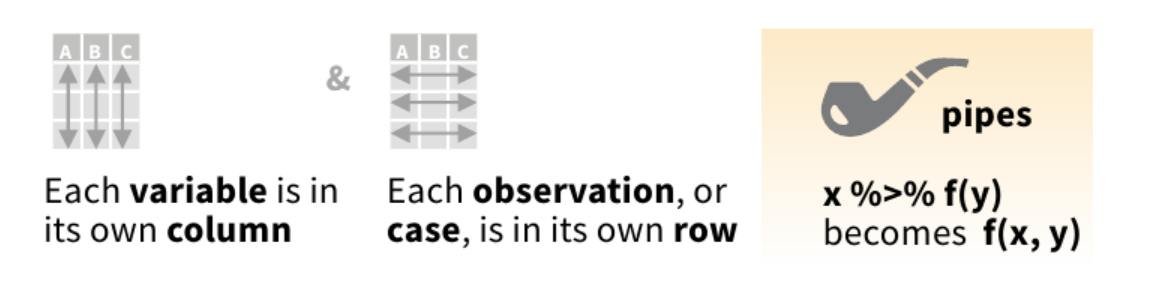
\includegraphics{img/da-dplyr/dplyr1.png}

Alternative way is to load \texttt{tidyverse} package with other
attached:

\begin{Shaded}
\begin{Highlighting}[]
\CommentTok{\# install.packages("tidyverse")}
\FunctionTok{library}\NormalTok{(tidyverse)}
\end{Highlighting}
\end{Shaded}

\begin{center}\rule{0.5\linewidth}{0.5pt}\end{center}

\section{Refences}\label{refences}

\begin{enumerate}
\def\labelenumi{\arabic{enumi}.}
\tightlist
\item
  \href{https://cran.r-project.org/web/packages/dplyr/index.html}{dplyr:
  A Grammar of Data Manipulation} on https://cran.r-project.org/.
\item
  \href{https://github.com/rstudio/cheatsheets/blob/master/data-transformation.pdf}{Data
  Transformation with splyr::cheat sheet}.
\item
  \href{https://www.listendata.com/2016/08/dplyr-tutorial.html}{DPLYR
  TUTORIAL : DATA MANIPULATION (50 EXAMPLES)} by Deepanshu Bhalla.
\item
  \href{https://stat545.com/dplyr-intro.html}{Dplyr Intro} by Stat 545.
  6.\href{https://www.guru99.com/r-dplyr-tutorial.html}{R Dplyr
  Tutorial: Data Manipulation(Join) \& Cleaning(Spread)}. Introduction
  to Data Analysis
\item
  \href{https://www.kaggle.com/kmldas/loan-default-prediction}{Loan
  Default Prediction. Beginners data set for financial analytics Kaggle}
\end{enumerate}

\chapter{\texorpdfstring{Exploring data with
\texttt{dplyr}}{Exploring data with dplyr}}\label{exploring-data-with-dplyr}

\begin{center}\rule{0.5\linewidth}{0.5pt}\end{center}

author: Юрій Клебан

\begin{center}\rule{0.5\linewidth}{0.5pt}\end{center}

\section{Basic funtions and dataset
explore}\label{basic-funtions-and-dataset-explore}

There are most popular functions in \texttt{dplyr} is listed in table.

\begin{longtable}[]{@{}lll@{}}
\toprule\noalign{}
dplyr Function & Description & Equivalent SQL \\
\midrule\noalign{}
\endhead
\bottomrule\noalign{}
\endlastfoot
select() & Selecting columns (variables) & SELECT \\
filter() & Filter (subset) rows. & WHERE \\
group\_by() & Group the data & GROUP BY \\
summarise() & Summarise (or aggregate) data & - \\
arrange() & Sort the data & ORDER BY \\
join() & Joining data frames (tables) & JOIN \\
mutate() & Creating New Variables & COLUMN ALIAS \\
\end{longtable}

For the next sample we are going to use \texttt{gapminder} dataset.
\hyperref[gapminder]{Go to gapminder dataset description}

The \texttt{gapminder} data frame include six variables:

\begin{longtable}[]{@{}ll@{}}
\toprule\noalign{}
variable & meaning \\
\midrule\noalign{}
\endhead
\bottomrule\noalign{}
\endlastfoot
country & - \\
continent & - \\
year & - \\
lifeExp & life expectancy at birth \\
pop & total population \\
gdpPercap & per-capita GDP \\
\end{longtable}

\texttt{Per-capita\ GDP} (Gross domestic product) is given in units of
international dollars,
\texttt{a\ hypothetical\ unit\ of\ currency\ that\ has\ the\ same\ purchasing\ power\ parity\ that\ the\ U.S.\ dollar\ had\ in\ the\ United\ States\ at\ a\ given\ point\ in\ time}
-- 2005, in this case.

The \texttt{gapminder} data frame is a special kind of data frame: a
\texttt{tibble}.

\begin{Shaded}
\begin{Highlighting}[]
\FunctionTok{library}\NormalTok{(dplyr) }\CommentTok{\# for demos}
\CommentTok{\#install.packages("gapminder")}
\FunctionTok{library}\NormalTok{(gapminder)  }\CommentTok{\# load package and dataset}
\FunctionTok{class}\NormalTok{(gapminder)}
\end{Highlighting}
\end{Shaded}

\begin{enumerate}
\def\labelenumi{\arabic{enumi}.}
\tightlist
\item
  `tbl\_df'
\item
  `tbl'
\item
  `data.frame'
\end{enumerate}

Let's preview it with functions \texttt{str()}, \texttt{glimpse()},
\texttt{head()}, \texttt{tail()}, \texttt{summary()}.

\begin{Shaded}
\begin{Highlighting}[]
\FunctionTok{str}\NormalTok{(gapminder)}
\end{Highlighting}
\end{Shaded}

\begin{verbatim}
tibble [1,704 x 6] (S3: tbl_df/tbl/data.frame)
 $ country  : Factor w/ 142 levels "Afghanistan",..: 1 1 1 1 1 1 1 1 1 1 ...
 $ continent: Factor w/ 5 levels "Africa","Americas",..: 3 3 3 3 3 3 3 3 3 3 ...
 $ year     : int [1:1704] 1952 1957 1962 1967 1972 1977 1982 1987 1992 1997 ...
 $ lifeExp  : num [1:1704] 28.8 30.3 32 34 36.1 ...
 $ pop      : int [1:1704] 8425333 9240934 10267083 11537966 13079460 14880372 12881816 13867957 16317921 22227415 ...
 $ gdpPercap: num [1:1704] 779 821 853 836 740 ...
\end{verbatim}

\begin{Shaded}
\begin{Highlighting}[]
\FunctionTok{glimpse}\NormalTok{(gapminder)}
\end{Highlighting}
\end{Shaded}

\begin{verbatim}
Rows: 1,704
Columns: 6
$ country   <fct> "Afghanistan", "Afghanistan", "Afghanistan", "Afghanistan", ~
$ continent <fct> Asia, Asia, Asia, Asia, Asia, Asia, Asia, Asia, Asia, Asia, ~
$ year      <int> 1952, 1957, 1962, 1967, 1972, 1977, 1982, 1987, 1992, 1997, ~
$ lifeExp   <dbl> 28.801, 30.332, 31.997, 34.020, 36.088, 38.438, 39.854, 40.8~
$ pop       <int> 8425333, 9240934, 10267083, 11537966, 13079460, 14880372, 12~
$ gdpPercap <dbl> 779.4453, 820.8530, 853.1007, 836.1971, 739.9811, 786.1134, ~
\end{verbatim}

\begin{Shaded}
\begin{Highlighting}[]
\FunctionTok{head}\NormalTok{(gapminder) }\CommentTok{\#shows first n{-}rows, 6 by default}
\end{Highlighting}
\end{Shaded}

A tibble: 6 × 6

\begin{longtable}[]{@{}
  >{\raggedright\arraybackslash}p{(\columnwidth - 10\tabcolsep) * \real{0.1667}}
  >{\raggedright\arraybackslash}p{(\columnwidth - 10\tabcolsep) * \real{0.1667}}
  >{\raggedright\arraybackslash}p{(\columnwidth - 10\tabcolsep) * \real{0.1667}}
  >{\raggedright\arraybackslash}p{(\columnwidth - 10\tabcolsep) * \real{0.1667}}
  >{\raggedright\arraybackslash}p{(\columnwidth - 10\tabcolsep) * \real{0.1667}}
  >{\raggedright\arraybackslash}p{(\columnwidth - 10\tabcolsep) * \real{0.1667}}@{}}
\toprule\noalign{}
\begin{minipage}[b]{\linewidth}\raggedright
country \textless fct\textgreater{}
\end{minipage} & \begin{minipage}[b]{\linewidth}\raggedright
continent \textless fct\textgreater{}
\end{minipage} & \begin{minipage}[b]{\linewidth}\raggedright
year \textless int\textgreater{}
\end{minipage} & \begin{minipage}[b]{\linewidth}\raggedright
lifeExp \textless dbl\textgreater{}
\end{minipage} & \begin{minipage}[b]{\linewidth}\raggedright
pop \textless int\textgreater{}
\end{minipage} & \begin{minipage}[b]{\linewidth}\raggedright
gdpPercap \textless dbl\textgreater{}
\end{minipage} \\
\midrule\noalign{}
\endhead
\bottomrule\noalign{}
\endlastfoot
Afghanistan & Asia & 1952 & 28.801 & 8425333 & 779.4453 \\
Afghanistan & Asia & 1957 & 30.332 & 9240934 & 820.8530 \\
Afghanistan & Asia & 1962 & 31.997 & 10267083 & 853.1007 \\
Afghanistan & Asia & 1967 & 34.020 & 11537966 & 836.1971 \\
Afghanistan & Asia & 1972 & 36.088 & 13079460 & 739.9811 \\
Afghanistan & Asia & 1977 & 38.438 & 14880372 & 786.1134 \\
\end{longtable}

\begin{Shaded}
\begin{Highlighting}[]
\FunctionTok{tail}\NormalTok{(gapminder) }\CommentTok{\#shows last n{-}rows, 6 by default}
\end{Highlighting}
\end{Shaded}

A tibble: 6 × 6

\begin{longtable}[]{@{}
  >{\raggedright\arraybackslash}p{(\columnwidth - 10\tabcolsep) * \real{0.1667}}
  >{\raggedright\arraybackslash}p{(\columnwidth - 10\tabcolsep) * \real{0.1667}}
  >{\raggedright\arraybackslash}p{(\columnwidth - 10\tabcolsep) * \real{0.1667}}
  >{\raggedright\arraybackslash}p{(\columnwidth - 10\tabcolsep) * \real{0.1667}}
  >{\raggedright\arraybackslash}p{(\columnwidth - 10\tabcolsep) * \real{0.1667}}
  >{\raggedright\arraybackslash}p{(\columnwidth - 10\tabcolsep) * \real{0.1667}}@{}}
\toprule\noalign{}
\begin{minipage}[b]{\linewidth}\raggedright
country \textless fct\textgreater{}
\end{minipage} & \begin{minipage}[b]{\linewidth}\raggedright
continent \textless fct\textgreater{}
\end{minipage} & \begin{minipage}[b]{\linewidth}\raggedright
year \textless int\textgreater{}
\end{minipage} & \begin{minipage}[b]{\linewidth}\raggedright
lifeExp \textless dbl\textgreater{}
\end{minipage} & \begin{minipage}[b]{\linewidth}\raggedright
pop \textless int\textgreater{}
\end{minipage} & \begin{minipage}[b]{\linewidth}\raggedright
gdpPercap \textless dbl\textgreater{}
\end{minipage} \\
\midrule\noalign{}
\endhead
\bottomrule\noalign{}
\endlastfoot
Zimbabwe & Africa & 1982 & 60.363 & 7636524 & 788.8550 \\
Zimbabwe & Africa & 1987 & 62.351 & 9216418 & 706.1573 \\
Zimbabwe & Africa & 1992 & 60.377 & 10704340 & 693.4208 \\
Zimbabwe & Africa & 1997 & 46.809 & 11404948 & 792.4500 \\
Zimbabwe & Africa & 2002 & 39.989 & 11926563 & 672.0386 \\
Zimbabwe & Africa & 2007 & 43.487 & 12311143 & 469.7093 \\
\end{longtable}

\begin{Shaded}
\begin{Highlighting}[]
\FunctionTok{summary}\NormalTok{(gapminder)}
\end{Highlighting}
\end{Shaded}

\begin{verbatim}
        country        continent        year         lifeExp     
 Afghanistan:  12   Africa  :624   Min.   :1952   Min.   :23.60  
 Albania    :  12   Americas:300   1st Qu.:1966   1st Qu.:48.20  
 Algeria    :  12   Asia    :396   Median :1980   Median :60.71  
 Angola     :  12   Europe  :360   Mean   :1980   Mean   :59.47  
 Argentina  :  12   Oceania : 24   3rd Qu.:1993   3rd Qu.:70.85  
 Australia  :  12                  Max.   :2007   Max.   :82.60  
 (Other)    :1632                                                
      pop              gdpPercap       
 Min.   :6.001e+04   Min.   :   241.2  
 1st Qu.:2.794e+06   1st Qu.:  1202.1  
 Median :7.024e+06   Median :  3531.8  
 Mean   :2.960e+07   Mean   :  7215.3  
 3rd Qu.:1.959e+07   3rd Qu.:  9325.5  
 Max.   :1.319e+09   Max.   :113523.1  
                                       
\end{verbatim}

\section{\texorpdfstring{\texttt{filter()}
function}{filter() function}}\label{filter-function}

\begin{Shaded}
\begin{Highlighting}[]
\NormalTok{austria }\OtherTok{\textless{}{-}} \FunctionTok{filter}\NormalTok{(gapminder, country }\SpecialCharTok{==} \StringTok{"Austria"}\NormalTok{)}
\NormalTok{austria}
\end{Highlighting}
\end{Shaded}

A tibble: 12 × 6

\begin{longtable}[]{@{}
  >{\raggedright\arraybackslash}p{(\columnwidth - 10\tabcolsep) * \real{0.1667}}
  >{\raggedright\arraybackslash}p{(\columnwidth - 10\tabcolsep) * \real{0.1667}}
  >{\raggedright\arraybackslash}p{(\columnwidth - 10\tabcolsep) * \real{0.1667}}
  >{\raggedright\arraybackslash}p{(\columnwidth - 10\tabcolsep) * \real{0.1667}}
  >{\raggedright\arraybackslash}p{(\columnwidth - 10\tabcolsep) * \real{0.1667}}
  >{\raggedright\arraybackslash}p{(\columnwidth - 10\tabcolsep) * \real{0.1667}}@{}}
\toprule\noalign{}
\begin{minipage}[b]{\linewidth}\raggedright
country \textless fct\textgreater{}
\end{minipage} & \begin{minipage}[b]{\linewidth}\raggedright
continent \textless fct\textgreater{}
\end{minipage} & \begin{minipage}[b]{\linewidth}\raggedright
year \textless int\textgreater{}
\end{minipage} & \begin{minipage}[b]{\linewidth}\raggedright
lifeExp \textless dbl\textgreater{}
\end{minipage} & \begin{minipage}[b]{\linewidth}\raggedright
pop \textless int\textgreater{}
\end{minipage} & \begin{minipage}[b]{\linewidth}\raggedright
gdpPercap \textless dbl\textgreater{}
\end{minipage} \\
\midrule\noalign{}
\endhead
\bottomrule\noalign{}
\endlastfoot
Austria & Europe & 1952 & 66.800 & 6927772 & 6137.076 \\
Austria & Europe & 1957 & 67.480 & 6965860 & 8842.598 \\
Austria & Europe & 1962 & 69.540 & 7129864 & 10750.721 \\
Austria & Europe & 1967 & 70.140 & 7376998 & 12834.602 \\
Austria & Europe & 1972 & 70.630 & 7544201 & 16661.626 \\
Austria & Europe & 1977 & 72.170 & 7568430 & 19749.422 \\
Austria & Europe & 1982 & 73.180 & 7574613 & 21597.084 \\
Austria & Europe & 1987 & 74.940 & 7578903 & 23687.826 \\
Austria & Europe & 1992 & 76.040 & 7914969 & 27042.019 \\
Austria & Europe & 1997 & 77.510 & 8069876 & 29095.921 \\
Austria & Europe & 2002 & 78.980 & 8148312 & 32417.608 \\
Austria & Europe & 2007 & 79.829 & 8199783 & 36126.493 \\
\end{longtable}

\texttt{filter()} takes logical expressions and returns the rows for
which all are TRUE.

\begin{Shaded}
\begin{Highlighting}[]
\CommentTok{\# task: select rows with lifeExp less than 31}
\FunctionTok{filter}\NormalTok{(gapminder, lifeExp }\SpecialCharTok{\textless{}} \DecValTok{31}\NormalTok{)}
\end{Highlighting}
\end{Shaded}

A tibble: 6 × 6

\begin{longtable}[]{@{}
  >{\raggedright\arraybackslash}p{(\columnwidth - 10\tabcolsep) * \real{0.1667}}
  >{\raggedright\arraybackslash}p{(\columnwidth - 10\tabcolsep) * \real{0.1667}}
  >{\raggedright\arraybackslash}p{(\columnwidth - 10\tabcolsep) * \real{0.1667}}
  >{\raggedright\arraybackslash}p{(\columnwidth - 10\tabcolsep) * \real{0.1667}}
  >{\raggedright\arraybackslash}p{(\columnwidth - 10\tabcolsep) * \real{0.1667}}
  >{\raggedright\arraybackslash}p{(\columnwidth - 10\tabcolsep) * \real{0.1667}}@{}}
\toprule\noalign{}
\begin{minipage}[b]{\linewidth}\raggedright
country \textless fct\textgreater{}
\end{minipage} & \begin{minipage}[b]{\linewidth}\raggedright
continent \textless fct\textgreater{}
\end{minipage} & \begin{minipage}[b]{\linewidth}\raggedright
year \textless int\textgreater{}
\end{minipage} & \begin{minipage}[b]{\linewidth}\raggedright
lifeExp \textless dbl\textgreater{}
\end{minipage} & \begin{minipage}[b]{\linewidth}\raggedright
pop \textless int\textgreater{}
\end{minipage} & \begin{minipage}[b]{\linewidth}\raggedright
gdpPercap \textless dbl\textgreater{}
\end{minipage} \\
\midrule\noalign{}
\endhead
\bottomrule\noalign{}
\endlastfoot
Afghanistan & Asia & 1952 & 28.801 & 8425333 & 779.4453 \\
Afghanistan & Asia & 1957 & 30.332 & 9240934 & 820.8530 \\
Angola & Africa & 1952 & 30.015 & 4232095 & 3520.6103 \\
Gambia & Africa & 1952 & 30.000 & 284320 & 485.2307 \\
Rwanda & Africa & 1992 & 23.599 & 7290203 & 737.0686 \\
Sierra Leone & Africa & 1952 & 30.331 & 2143249 & 879.7877 \\
\end{longtable}

\begin{Shaded}
\begin{Highlighting}[]
\CommentTok{\# task: select Austria only and year after 1980}
\FunctionTok{filter}\NormalTok{(gapminder, country }\SpecialCharTok{==} \StringTok{"Austria"}\NormalTok{, year }\SpecialCharTok{\textgreater{}} \DecValTok{1980}\NormalTok{)}
\end{Highlighting}
\end{Shaded}

A tibble: 6 × 6

\begin{longtable}[]{@{}
  >{\raggedright\arraybackslash}p{(\columnwidth - 10\tabcolsep) * \real{0.1667}}
  >{\raggedright\arraybackslash}p{(\columnwidth - 10\tabcolsep) * \real{0.1667}}
  >{\raggedright\arraybackslash}p{(\columnwidth - 10\tabcolsep) * \real{0.1667}}
  >{\raggedright\arraybackslash}p{(\columnwidth - 10\tabcolsep) * \real{0.1667}}
  >{\raggedright\arraybackslash}p{(\columnwidth - 10\tabcolsep) * \real{0.1667}}
  >{\raggedright\arraybackslash}p{(\columnwidth - 10\tabcolsep) * \real{0.1667}}@{}}
\toprule\noalign{}
\begin{minipage}[b]{\linewidth}\raggedright
country \textless fct\textgreater{}
\end{minipage} & \begin{minipage}[b]{\linewidth}\raggedright
continent \textless fct\textgreater{}
\end{minipage} & \begin{minipage}[b]{\linewidth}\raggedright
year \textless int\textgreater{}
\end{minipage} & \begin{minipage}[b]{\linewidth}\raggedright
lifeExp \textless dbl\textgreater{}
\end{minipage} & \begin{minipage}[b]{\linewidth}\raggedright
pop \textless int\textgreater{}
\end{minipage} & \begin{minipage}[b]{\linewidth}\raggedright
gdpPercap \textless dbl\textgreater{}
\end{minipage} \\
\midrule\noalign{}
\endhead
\bottomrule\noalign{}
\endlastfoot
Austria & Europe & 1982 & 73.180 & 7574613 & 21597.08 \\
Austria & Europe & 1987 & 74.940 & 7578903 & 23687.83 \\
Austria & Europe & 1992 & 76.040 & 7914969 & 27042.02 \\
Austria & Europe & 1997 & 77.510 & 8069876 & 29095.92 \\
Austria & Europe & 2002 & 78.980 & 8148312 & 32417.61 \\
Austria & Europe & 2007 & 79.829 & 8199783 & 36126.49 \\
\end{longtable}

\begin{Shaded}
\begin{Highlighting}[]
\CommentTok{\# task: select Austria and Belgium}
\FunctionTok{filter}\NormalTok{(gapminder, country }\SpecialCharTok{\%in\%} \FunctionTok{c}\NormalTok{(}\StringTok{"Austria"}\NormalTok{, }\StringTok{"Belgium"}\NormalTok{))}
\end{Highlighting}
\end{Shaded}

A tibble: 24 × 6

\begin{longtable}[]{@{}
  >{\raggedright\arraybackslash}p{(\columnwidth - 10\tabcolsep) * \real{0.1667}}
  >{\raggedright\arraybackslash}p{(\columnwidth - 10\tabcolsep) * \real{0.1667}}
  >{\raggedright\arraybackslash}p{(\columnwidth - 10\tabcolsep) * \real{0.1667}}
  >{\raggedright\arraybackslash}p{(\columnwidth - 10\tabcolsep) * \real{0.1667}}
  >{\raggedright\arraybackslash}p{(\columnwidth - 10\tabcolsep) * \real{0.1667}}
  >{\raggedright\arraybackslash}p{(\columnwidth - 10\tabcolsep) * \real{0.1667}}@{}}
\toprule\noalign{}
\begin{minipage}[b]{\linewidth}\raggedright
country \textless fct\textgreater{}
\end{minipage} & \begin{minipage}[b]{\linewidth}\raggedright
continent \textless fct\textgreater{}
\end{minipage} & \begin{minipage}[b]{\linewidth}\raggedright
year \textless int\textgreater{}
\end{minipage} & \begin{minipage}[b]{\linewidth}\raggedright
lifeExp \textless dbl\textgreater{}
\end{minipage} & \begin{minipage}[b]{\linewidth}\raggedright
pop \textless int\textgreater{}
\end{minipage} & \begin{minipage}[b]{\linewidth}\raggedright
gdpPercap \textless dbl\textgreater{}
\end{minipage} \\
\midrule\noalign{}
\endhead
\bottomrule\noalign{}
\endlastfoot
Austria & Europe & 1952 & 66.800 & 6927772 & 6137.076 \\
Austria & Europe & 1957 & 67.480 & 6965860 & 8842.598 \\
Austria & Europe & 1962 & 69.540 & 7129864 & 10750.721 \\
Austria & Europe & 1967 & 70.140 & 7376998 & 12834.602 \\
Austria & Europe & 1972 & 70.630 & 7544201 & 16661.626 \\
Austria & Europe & 1977 & 72.170 & 7568430 & 19749.422 \\
Austria & Europe & 1982 & 73.180 & 7574613 & 21597.084 \\
Austria & Europe & 1987 & 74.940 & 7578903 & 23687.826 \\
Austria & Europe & 1992 & 76.040 & 7914969 & 27042.019 \\
Austria & Europe & 1997 & 77.510 & 8069876 & 29095.921 \\
Austria & Europe & 2002 & 78.980 & 8148312 & 32417.608 \\
Austria & Europe & 2007 & 79.829 & 8199783 & 36126.493 \\
Belgium & Europe & 1952 & 68.000 & 8730405 & 8343.105 \\
Belgium & Europe & 1957 & 69.240 & 8989111 & 9714.961 \\
Belgium & Europe & 1962 & 70.250 & 9218400 & 10991.207 \\
Belgium & Europe & 1967 & 70.940 & 9556500 & 13149.041 \\
Belgium & Europe & 1972 & 71.440 & 9709100 & 16672.144 \\
Belgium & Europe & 1977 & 72.800 & 9821800 & 19117.974 \\
Belgium & Europe & 1982 & 73.930 & 9856303 & 20979.846 \\
Belgium & Europe & 1987 & 75.350 & 9870200 & 22525.563 \\
Belgium & Europe & 1992 & 76.460 & 10045622 & 25575.571 \\
Belgium & Europe & 1997 & 77.530 & 10199787 & 27561.197 \\
Belgium & Europe & 2002 & 78.320 & 10311970 & 30485.884 \\
Belgium & Europe & 2007 & 79.441 & 10392226 & 33692.605 \\
\end{longtable}

Lets rewrite initial code and record it to the variable/data.frame:

\section{\texorpdfstring{Pipe
(\texttt{\%\textgreater{}\%}/\texttt{\textbar{}\textgreater{}})
operator}{Pipe (\%\textgreater\%/\textbar\textgreater) operator}}\label{pipe-operator}

\texttt{\%\textgreater{}\%} is \texttt{pipe} operator. The pipe operator
takes the thing on the left-hand-side and pipes it into the function
call on the right-hand-side -- literally, drops it in as the first
argument.

\texttt{head()} function without pipe and top 4 items:

\begin{quote}
In R version before 4.1.0 \texttt{pipe} \texttt{\%\textgreater{}\%}
operator is not a language build-in and you should install
\texttt{magrittr} package:
\end{quote}

\begin{quote}
\textbf{Pipe opertor in R 4.1+ \texttt{\textbar{}\textgreater{}}, using
this is preferable}
\end{quote}

\begin{Shaded}
\begin{Highlighting}[]
\CommentTok{\#install.packages("magrittr") \# for pipe \%\textgreater{}\% operator}
\FunctionTok{library}\NormalTok{(magrittr)}
\end{Highlighting}
\end{Shaded}

\begin{Shaded}
\begin{Highlighting}[]
\FunctionTok{head}\NormalTok{(gapminder, }\AttributeTok{n =} \DecValTok{4}\NormalTok{)}
\end{Highlighting}
\end{Shaded}

A tibble: 4 × 6

\begin{longtable}[]{@{}
  >{\raggedright\arraybackslash}p{(\columnwidth - 10\tabcolsep) * \real{0.1667}}
  >{\raggedright\arraybackslash}p{(\columnwidth - 10\tabcolsep) * \real{0.1667}}
  >{\raggedright\arraybackslash}p{(\columnwidth - 10\tabcolsep) * \real{0.1667}}
  >{\raggedright\arraybackslash}p{(\columnwidth - 10\tabcolsep) * \real{0.1667}}
  >{\raggedright\arraybackslash}p{(\columnwidth - 10\tabcolsep) * \real{0.1667}}
  >{\raggedright\arraybackslash}p{(\columnwidth - 10\tabcolsep) * \real{0.1667}}@{}}
\toprule\noalign{}
\begin{minipage}[b]{\linewidth}\raggedright
country \textless fct\textgreater{}
\end{minipage} & \begin{minipage}[b]{\linewidth}\raggedright
continent \textless fct\textgreater{}
\end{minipage} & \begin{minipage}[b]{\linewidth}\raggedright
year \textless int\textgreater{}
\end{minipage} & \begin{minipage}[b]{\linewidth}\raggedright
lifeExp \textless dbl\textgreater{}
\end{minipage} & \begin{minipage}[b]{\linewidth}\raggedright
pop \textless int\textgreater{}
\end{minipage} & \begin{minipage}[b]{\linewidth}\raggedright
gdpPercap \textless dbl\textgreater{}
\end{minipage} \\
\midrule\noalign{}
\endhead
\bottomrule\noalign{}
\endlastfoot
Afghanistan & Asia & 1952 & 28.801 & 8425333 & 779.4453 \\
Afghanistan & Asia & 1957 & 30.332 & 9240934 & 820.8530 \\
Afghanistan & Asia & 1962 & 31.997 & 10267083 & 853.1007 \\
Afghanistan & Asia & 1967 & 34.020 & 11537966 & 836.1971 \\
\end{longtable}

\texttt{head()} function with pipe and top 4 items:

\begin{Shaded}
\begin{Highlighting}[]
\NormalTok{gapminder }\SpecialCharTok{\%\textgreater{}\%} \FunctionTok{head}\NormalTok{(}\DecValTok{4}\NormalTok{)}
\end{Highlighting}
\end{Shaded}

A tibble: 4 × 6

\begin{longtable}[]{@{}
  >{\raggedright\arraybackslash}p{(\columnwidth - 10\tabcolsep) * \real{0.1667}}
  >{\raggedright\arraybackslash}p{(\columnwidth - 10\tabcolsep) * \real{0.1667}}
  >{\raggedright\arraybackslash}p{(\columnwidth - 10\tabcolsep) * \real{0.1667}}
  >{\raggedright\arraybackslash}p{(\columnwidth - 10\tabcolsep) * \real{0.1667}}
  >{\raggedright\arraybackslash}p{(\columnwidth - 10\tabcolsep) * \real{0.1667}}
  >{\raggedright\arraybackslash}p{(\columnwidth - 10\tabcolsep) * \real{0.1667}}@{}}
\toprule\noalign{}
\begin{minipage}[b]{\linewidth}\raggedright
country \textless fct\textgreater{}
\end{minipage} & \begin{minipage}[b]{\linewidth}\raggedright
continent \textless fct\textgreater{}
\end{minipage} & \begin{minipage}[b]{\linewidth}\raggedright
year \textless int\textgreater{}
\end{minipage} & \begin{minipage}[b]{\linewidth}\raggedright
lifeExp \textless dbl\textgreater{}
\end{minipage} & \begin{minipage}[b]{\linewidth}\raggedright
pop \textless int\textgreater{}
\end{minipage} & \begin{minipage}[b]{\linewidth}\raggedright
gdpPercap \textless dbl\textgreater{}
\end{minipage} \\
\midrule\noalign{}
\endhead
\bottomrule\noalign{}
\endlastfoot
Afghanistan & Asia & 1952 & 28.801 & 8425333 & 779.4453 \\
Afghanistan & Asia & 1957 & 30.332 & 9240934 & 820.8530 \\
Afghanistan & Asia & 1962 & 31.997 & 10267083 & 853.1007 \\
Afghanistan & Asia & 1967 & 34.020 & 11537966 & 836.1971 \\
\end{longtable}

Output is the same. So, let's rewrire filtering for \texttt{Austria}
with pipe:

\begin{Shaded}
\begin{Highlighting}[]
\NormalTok{austria }\OtherTok{\textless{}{-}}\NormalTok{ gapminder }\SpecialCharTok{|\textgreater{}} \FunctionTok{filter}\NormalTok{(country }\SpecialCharTok{==} \StringTok{"Austria"}\NormalTok{)}
\NormalTok{austria}
\end{Highlighting}
\end{Shaded}

A tibble: 12 × 6

\begin{longtable}[]{@{}
  >{\raggedright\arraybackslash}p{(\columnwidth - 10\tabcolsep) * \real{0.1667}}
  >{\raggedright\arraybackslash}p{(\columnwidth - 10\tabcolsep) * \real{0.1667}}
  >{\raggedright\arraybackslash}p{(\columnwidth - 10\tabcolsep) * \real{0.1667}}
  >{\raggedright\arraybackslash}p{(\columnwidth - 10\tabcolsep) * \real{0.1667}}
  >{\raggedright\arraybackslash}p{(\columnwidth - 10\tabcolsep) * \real{0.1667}}
  >{\raggedright\arraybackslash}p{(\columnwidth - 10\tabcolsep) * \real{0.1667}}@{}}
\toprule\noalign{}
\begin{minipage}[b]{\linewidth}\raggedright
country \textless fct\textgreater{}
\end{minipage} & \begin{minipage}[b]{\linewidth}\raggedright
continent \textless fct\textgreater{}
\end{minipage} & \begin{minipage}[b]{\linewidth}\raggedright
year \textless int\textgreater{}
\end{minipage} & \begin{minipage}[b]{\linewidth}\raggedright
lifeExp \textless dbl\textgreater{}
\end{minipage} & \begin{minipage}[b]{\linewidth}\raggedright
pop \textless int\textgreater{}
\end{minipage} & \begin{minipage}[b]{\linewidth}\raggedright
gdpPercap \textless dbl\textgreater{}
\end{minipage} \\
\midrule\noalign{}
\endhead
\bottomrule\noalign{}
\endlastfoot
Austria & Europe & 1952 & 66.800 & 6927772 & 6137.076 \\
Austria & Europe & 1957 & 67.480 & 6965860 & 8842.598 \\
Austria & Europe & 1962 & 69.540 & 7129864 & 10750.721 \\
Austria & Europe & 1967 & 70.140 & 7376998 & 12834.602 \\
Austria & Europe & 1972 & 70.630 & 7544201 & 16661.626 \\
Austria & Europe & 1977 & 72.170 & 7568430 & 19749.422 \\
Austria & Europe & 1982 & 73.180 & 7574613 & 21597.084 \\
Austria & Europe & 1987 & 74.940 & 7578903 & 23687.826 \\
Austria & Europe & 1992 & 76.040 & 7914969 & 27042.019 \\
Austria & Europe & 1997 & 77.510 & 8069876 & 29095.921 \\
Austria & Europe & 2002 & 78.980 & 8148312 & 32417.608 \\
Austria & Europe & 2007 & 79.829 & 8199783 & 36126.493 \\
\end{longtable}

\begin{Shaded}
\begin{Highlighting}[]
\CommentTok{\# add more conditions in filter}
\NormalTok{austria }\OtherTok{\textless{}{-}}\NormalTok{ gapminder }\SpecialCharTok{|\textgreater{}} \FunctionTok{filter}\NormalTok{(country }\SpecialCharTok{==} \StringTok{"Austria"}\NormalTok{, year }\SpecialCharTok{\textgreater{}} \DecValTok{2000}\NormalTok{)}
\NormalTok{austria}
\end{Highlighting}
\end{Shaded}

A tibble: 2 × 6

\begin{longtable}[]{@{}
  >{\raggedright\arraybackslash}p{(\columnwidth - 10\tabcolsep) * \real{0.1667}}
  >{\raggedright\arraybackslash}p{(\columnwidth - 10\tabcolsep) * \real{0.1667}}
  >{\raggedright\arraybackslash}p{(\columnwidth - 10\tabcolsep) * \real{0.1667}}
  >{\raggedright\arraybackslash}p{(\columnwidth - 10\tabcolsep) * \real{0.1667}}
  >{\raggedright\arraybackslash}p{(\columnwidth - 10\tabcolsep) * \real{0.1667}}
  >{\raggedright\arraybackslash}p{(\columnwidth - 10\tabcolsep) * \real{0.1667}}@{}}
\toprule\noalign{}
\begin{minipage}[b]{\linewidth}\raggedright
country \textless fct\textgreater{}
\end{minipage} & \begin{minipage}[b]{\linewidth}\raggedright
continent \textless fct\textgreater{}
\end{minipage} & \begin{minipage}[b]{\linewidth}\raggedright
year \textless int\textgreater{}
\end{minipage} & \begin{minipage}[b]{\linewidth}\raggedright
lifeExp \textless dbl\textgreater{}
\end{minipage} & \begin{minipage}[b]{\linewidth}\raggedright
pop \textless int\textgreater{}
\end{minipage} & \begin{minipage}[b]{\linewidth}\raggedright
gdpPercap \textless dbl\textgreater{}
\end{minipage} \\
\midrule\noalign{}
\endhead
\bottomrule\noalign{}
\endlastfoot
Austria & Europe & 2002 & 78.980 & 8148312 & 32417.61 \\
Austria & Europe & 2007 & 79.829 & 8199783 & 36126.49 \\
\end{longtable}

\begin{center}\rule{0.5\linewidth}{0.5pt}\end{center}

\section{\texorpdfstring{\texttt{select()}
function}{select() function}}\label{select-function}

Use \texttt{select()} to subset the data on variables/columns by
\texttt{names} or \texttt{index}. You also can define order of columns
with \texttt{select()}.

\begin{Shaded}
\begin{Highlighting}[]
\NormalTok{gapminder }\SpecialCharTok{|\textgreater{}} 
\FunctionTok{select}\NormalTok{(year, country, pop) }\SpecialCharTok{|\textgreater{}}
\FunctionTok{slice}\NormalTok{(}\DecValTok{1}\SpecialCharTok{:} \DecValTok{10}\NormalTok{)}
\end{Highlighting}
\end{Shaded}

A tibble: 10 × 3

\begin{longtable}[]{@{}lll@{}}
\toprule\noalign{}
year \textless int\textgreater{} & country \textless fct\textgreater{} &
pop \textless int\textgreater{} \\
\midrule\noalign{}
\endhead
\bottomrule\noalign{}
\endlastfoot
1952 & Afghanistan & 8425333 \\
1957 & Afghanistan & 9240934 \\
1962 & Afghanistan & 10267083 \\
1967 & Afghanistan & 11537966 \\
1972 & Afghanistan & 13079460 \\
1977 & Afghanistan & 14880372 \\
1982 & Afghanistan & 12881816 \\
1987 & Afghanistan & 13867957 \\
1992 & Afghanistan & 16317921 \\
1997 & Afghanistan & 22227415 \\
\end{longtable}

Lets combine few functions with \texttt{pipe}
(\texttt{\%\textgreater{}\%}):

Finally, lest extend our filtering:

\begin{Shaded}
\begin{Highlighting}[]
\CommentTok{\# compare dplyr syntax with base R call}
\NormalTok{gapminder[gapminder}\SpecialCharTok{$}\NormalTok{country }\SpecialCharTok{==} \StringTok{"Austria"}\NormalTok{, }\FunctionTok{c}\NormalTok{(}\StringTok{"year"}\NormalTok{, }\StringTok{"pop"}\NormalTok{, }\StringTok{"lifeExp"}\NormalTok{)]}

\NormalTok{gapminder }\SpecialCharTok{|\textgreater{}} 
    \FunctionTok{filter}\NormalTok{(country }\SpecialCharTok{==} \StringTok{"Austria"}\NormalTok{) }\SpecialCharTok{|\textgreater{}}
    \FunctionTok{select}\NormalTok{(year, pop, lifeExp)}
\end{Highlighting}
\end{Shaded}

A tibble: 12 × 3

\begin{longtable}[]{@{}lll@{}}
\toprule\noalign{}
year \textless int\textgreater{} & pop \textless int\textgreater{} &
lifeExp \textless dbl\textgreater{} \\
\midrule\noalign{}
\endhead
\bottomrule\noalign{}
\endlastfoot
1952 & 6927772 & 66.800 \\
1957 & 6965860 & 67.480 \\
1962 & 7129864 & 69.540 \\
1967 & 7376998 & 70.140 \\
1972 & 7544201 & 70.630 \\
1977 & 7568430 & 72.170 \\
1982 & 7574613 & 73.180 \\
1987 & 7578903 & 74.940 \\
1992 & 7914969 & 76.040 \\
1997 & 8069876 & 77.510 \\
2002 & 8148312 & 78.980 \\
2007 & 8199783 & 79.829 \\
\end{longtable}

A tibble: 12 × 3

\begin{longtable}[]{@{}lll@{}}
\toprule\noalign{}
year \textless int\textgreater{} & pop \textless int\textgreater{} &
lifeExp \textless dbl\textgreater{} \\
\midrule\noalign{}
\endhead
\bottomrule\noalign{}
\endlastfoot
1952 & 6927772 & 66.800 \\
1957 & 6965860 & 67.480 \\
1962 & 7129864 & 69.540 \\
1967 & 7376998 & 70.140 \\
1972 & 7544201 & 70.630 \\
1977 & 7568430 & 72.170 \\
1982 & 7574613 & 73.180 \\
1987 & 7578903 & 74.940 \\
1992 & 7914969 & 76.040 \\
1997 & 8069876 & 77.510 \\
2002 & 8148312 & 78.980 \\
2007 & 8199783 & 79.829 \\
\end{longtable}

You can remove some columns using \texttt{minus}(operator) and add few
filter conditions:

\begin{Shaded}
\begin{Highlighting}[]
\NormalTok{austria }\OtherTok{\textless{}{-}}\NormalTok{ gapminder }\SpecialCharTok{|\textgreater{}} 
                \FunctionTok{filter}\NormalTok{(country }\SpecialCharTok{==} \StringTok{"Austria"}\NormalTok{, year }\SpecialCharTok{\textgreater{}} \DecValTok{2000}\NormalTok{) }\SpecialCharTok{|\textgreater{}}
                \FunctionTok{select}\NormalTok{(}\SpecialCharTok{{-}}\NormalTok{continent, }\SpecialCharTok{{-}}\NormalTok{gdpPercap) }\SpecialCharTok{|\textgreater{}}
                \FunctionTok{head}\NormalTok{()}
\NormalTok{austria}
\end{Highlighting}
\end{Shaded}

A tibble: 2 × 4

\begin{longtable}[]{@{}
  >{\raggedright\arraybackslash}p{(\columnwidth - 6\tabcolsep) * \real{0.2500}}
  >{\raggedright\arraybackslash}p{(\columnwidth - 6\tabcolsep) * \real{0.2500}}
  >{\raggedright\arraybackslash}p{(\columnwidth - 6\tabcolsep) * \real{0.2500}}
  >{\raggedright\arraybackslash}p{(\columnwidth - 6\tabcolsep) * \real{0.2500}}@{}}
\toprule\noalign{}
\begin{minipage}[b]{\linewidth}\raggedright
country \textless fct\textgreater{}
\end{minipage} & \begin{minipage}[b]{\linewidth}\raggedright
year \textless int\textgreater{}
\end{minipage} & \begin{minipage}[b]{\linewidth}\raggedright
lifeExp \textless dbl\textgreater{}
\end{minipage} & \begin{minipage}[b]{\linewidth}\raggedright
pop \textless int\textgreater{}
\end{minipage} \\
\midrule\noalign{}
\endhead
\bottomrule\noalign{}
\endlastfoot
Austria & 2002 & 78.980 & 8148312 \\
Austria & 2007 & 79.829 & 8199783 \\
\end{longtable}

You can insert different conditions about columns you need to
\texttt{select}.

\begin{Shaded}
\begin{Highlighting}[]
\NormalTok{gapminder }\SpecialCharTok{|\textgreater{}}
    \FunctionTok{select}\NormalTok{(}\SpecialCharTok{!}\FunctionTok{where}\NormalTok{(is.numeric)) }\SpecialCharTok{|\textgreater{}}  \CommentTok{\# its 1704 records, because of repeating some records}
    \FunctionTok{slice}\NormalTok{(}\DecValTok{1}\SpecialCharTok{:}\DecValTok{5}\NormalTok{)}
\end{Highlighting}
\end{Shaded}

A tibble: 5 × 2

\begin{longtable}[]{@{}ll@{}}
\toprule\noalign{}
country \textless fct\textgreater{} & continent
\textless fct\textgreater{} \\
\midrule\noalign{}
\endhead
\bottomrule\noalign{}
\endlastfoot
Afghanistan & Asia \\
Afghanistan & Asia \\
Afghanistan & Asia \\
Afghanistan & Asia \\
Afghanistan & Asia \\
\end{longtable}

Let's output all unique pairs
\texttt{continent\ -\textgreater{}\ country} with \texttt{distinct()}
function:

\begin{Shaded}
\begin{Highlighting}[]
\NormalTok{gapminder }\SpecialCharTok{|\textgreater{}}
    \FunctionTok{select}\NormalTok{(country) }\SpecialCharTok{|\textgreater{}}
    \FunctionTok{distinct}\NormalTok{() }\CommentTok{\# its 142 records now}
\end{Highlighting}
\end{Shaded}

A tibble: 142 × 1

\begin{longtable}[]{@{}l@{}}
\toprule\noalign{}
country \textless fct\textgreater{} \\
\midrule\noalign{}
\endhead
\bottomrule\noalign{}
\endlastfoot
Afghanistan \\
Albania \\
Algeria \\
Angola \\
Argentina \\
Australia \\
Austria \\
Bahrain \\
Bangladesh \\
Belgium \\
Benin \\
Bolivia \\
Bosnia and Herzegovina \\
Botswana \\
Brazil \\
Bulgaria \\
Burkina Faso \\
Burundi \\
Cambodia \\
Cameroon \\
Canada \\
Central African Republic \\
Chad \\
Chile \\
China \\
Colombia \\
Comoros \\
Congo, Dem. Rep. \\
Congo, Rep. \\
Costa Rica \\
⋮ \\
Sierra Leone \\
Singapore \\
Slovak Republic \\
Slovenia \\
Somalia \\
South Africa \\
Spain \\
Sri Lanka \\
Sudan \\
Swaziland \\
Sweden \\
Switzerland \\
Syria \\
Taiwan \\
Tanzania \\
Thailand \\
Togo \\
Trinidad and Tobago \\
Tunisia \\
Turkey \\
Uganda \\
United Kingdom \\
United States \\
Uruguay \\
Venezuela \\
Vietnam \\
West Bank and Gaza \\
Yemen, Rep. \\
Zambia \\
Zimbabwe \\
\end{longtable}

\begin{center}\rule{0.5\linewidth}{0.5pt}\end{center}

\section{\texorpdfstring{Selecting random \(N\)
rows}{Selecting random N rows}}\label{selecting-random-n-rows}

The \texttt{sample\_n()} function selects random rows from a data frame

\begin{Shaded}
\begin{Highlighting}[]
\NormalTok{gapminder }\SpecialCharTok{|\textgreater{}} \FunctionTok{sample\_n}\NormalTok{(}\DecValTok{5}\NormalTok{)}
\end{Highlighting}
\end{Shaded}

A tibble: 5 × 6

\begin{longtable}[]{@{}
  >{\raggedright\arraybackslash}p{(\columnwidth - 10\tabcolsep) * \real{0.1667}}
  >{\raggedright\arraybackslash}p{(\columnwidth - 10\tabcolsep) * \real{0.1667}}
  >{\raggedright\arraybackslash}p{(\columnwidth - 10\tabcolsep) * \real{0.1667}}
  >{\raggedright\arraybackslash}p{(\columnwidth - 10\tabcolsep) * \real{0.1667}}
  >{\raggedright\arraybackslash}p{(\columnwidth - 10\tabcolsep) * \real{0.1667}}
  >{\raggedright\arraybackslash}p{(\columnwidth - 10\tabcolsep) * \real{0.1667}}@{}}
\toprule\noalign{}
\begin{minipage}[b]{\linewidth}\raggedright
country \textless fct\textgreater{}
\end{minipage} & \begin{minipage}[b]{\linewidth}\raggedright
continent \textless fct\textgreater{}
\end{minipage} & \begin{minipage}[b]{\linewidth}\raggedright
year \textless int\textgreater{}
\end{minipage} & \begin{minipage}[b]{\linewidth}\raggedright
lifeExp \textless dbl\textgreater{}
\end{minipage} & \begin{minipage}[b]{\linewidth}\raggedright
pop \textless int\textgreater{}
\end{minipage} & \begin{minipage}[b]{\linewidth}\raggedright
gdpPercap \textless dbl\textgreater{}
\end{minipage} \\
\midrule\noalign{}
\endhead
\bottomrule\noalign{}
\endlastfoot
Norway & Europe & 1967 & 74.080 & 3786019 & 16361.8765 \\
Central African Republic & Africa & 2002 & 43.308 & 4048013 &
738.6906 \\
Uruguay & Americas & 2007 & 76.384 & 3447496 & 10611.4630 \\
Togo & Africa & 1997 & 58.390 & 4320890 & 982.2869 \\
Paraguay & Americas & 2002 & 70.755 & 5884491 & 3783.6742 \\
\end{longtable}

If you want make \texttt{pseudo-random\ generation} reprodusable use
\texttt{set.seed()}. Seed is start point of random generation. Different
seeds give different output.

\begin{Shaded}
\begin{Highlighting}[]
\FunctionTok{set.seed}\NormalTok{(}\DecValTok{2023}\NormalTok{) }\CommentTok{\# example, seed = 2023}
\end{Highlighting}
\end{Shaded}

The \texttt{sample\_frac()} function selects random fraction rows from a
data frame. Let's select \(1\%\) of data

\begin{Shaded}
\begin{Highlighting}[]
\FunctionTok{set.seed}\NormalTok{(}\DecValTok{2023}\NormalTok{) }\CommentTok{\# output not changing, uncomment it }
\NormalTok{gapminder }\SpecialCharTok{\%\textgreater{}\%} \FunctionTok{sample\_frac}\NormalTok{(}\FloatTok{0.1}\NormalTok{)}
\end{Highlighting}
\end{Shaded}

A tibble: 170 × 6

\begin{longtable}[]{@{}
  >{\raggedright\arraybackslash}p{(\columnwidth - 10\tabcolsep) * \real{0.1667}}
  >{\raggedright\arraybackslash}p{(\columnwidth - 10\tabcolsep) * \real{0.1667}}
  >{\raggedright\arraybackslash}p{(\columnwidth - 10\tabcolsep) * \real{0.1667}}
  >{\raggedright\arraybackslash}p{(\columnwidth - 10\tabcolsep) * \real{0.1667}}
  >{\raggedright\arraybackslash}p{(\columnwidth - 10\tabcolsep) * \real{0.1667}}
  >{\raggedright\arraybackslash}p{(\columnwidth - 10\tabcolsep) * \real{0.1667}}@{}}
\toprule\noalign{}
\begin{minipage}[b]{\linewidth}\raggedright
country \textless fct\textgreater{}
\end{minipage} & \begin{minipage}[b]{\linewidth}\raggedright
continent \textless fct\textgreater{}
\end{minipage} & \begin{minipage}[b]{\linewidth}\raggedright
year \textless int\textgreater{}
\end{minipage} & \begin{minipage}[b]{\linewidth}\raggedright
lifeExp \textless dbl\textgreater{}
\end{minipage} & \begin{minipage}[b]{\linewidth}\raggedright
pop \textless int\textgreater{}
\end{minipage} & \begin{minipage}[b]{\linewidth}\raggedright
gdpPercap \textless dbl\textgreater{}
\end{minipage} \\
\midrule\noalign{}
\endhead
\bottomrule\noalign{}
\endlastfoot
Switzerland & Europe & 2007 & 81.701 & 7554661 & 37506.4191 \\
Djibouti & Africa & 2002 & 53.373 & 447416 & 1908.2609 \\
Slovenia & Europe & 1972 & 69.820 & 1694510 & 12383.4862 \\
Sao Tome and Principe & Africa & 1997 & 63.306 & 145608 & 1339.0760 \\
Turkey & Europe & 1987 & 63.108 & 52881328 & 5089.0437 \\
Lebanon & Asia & 1957 & 59.489 & 1647412 & 6089.7869 \\
Eritrea & Africa & 1972 & 44.142 & 2260187 & 514.3242 \\
Philippines & Asia & 1972 & 58.065 & 40850141 & 1989.3741 \\
Tunisia & Africa & 1972 & 55.602 & 5303507 & 2753.2860 \\
Uganda & Africa & 1952 & 39.978 & 5824797 & 734.7535 \\
Oman & Asia & 1972 & 52.143 & 829050 & 10618.0385 \\
Australia & Oceania & 2007 & 81.235 & 20434176 & 34435.3674 \\
Mali & Africa & 2002 & 51.818 & 10580176 & 951.4098 \\
Equatorial Guinea & Africa & 1957 & 35.983 & 232922 & 426.0964 \\
South Africa & Africa & 1982 & 58.161 & 31140029 & 8568.2662 \\
Burundi & Africa & 1962 & 42.045 & 2961915 & 355.2032 \\
Angola & Africa & 1992 & 40.647 & 8735988 & 2627.8457 \\
Yemen, Rep. & Asia & 1952 & 32.548 & 4963829 & 781.7176 \\
Croatia & Europe & 2007 & 75.748 & 4493312 & 14619.2227 \\
Oman & Asia & 1992 & 71.197 & 1915208 & 18616.7069 \\
Thailand & Asia & 1962 & 56.061 & 29263397 & 1002.1992 \\
Comoros & Africa & 1952 & 40.715 & 153936 & 1102.9909 \\
Eritrea & Africa & 1957 & 38.047 & 1542611 & 344.1619 \\
Zambia & Africa & 2002 & 39.193 & 10595811 & 1071.6139 \\
Cote d'Ivoire & Africa & 1987 & 54.655 & 10761098 & 2156.9561 \\
South Africa & Africa & 1957 & 47.985 & 16151549 & 5487.1042 \\
Paraguay & Americas & 1957 & 63.196 & 1770902 & 2046.1547 \\
Kuwait & Asia & 1952 & 55.565 & 160000 & 108382.3529 \\
Brazil & Americas & 1952 & 50.917 & 56602560 & 2108.9444 \\
Canada & Americas & 1957 & 69.960 & 17010154 & 12489.9501 \\
⋮ & ⋮ & ⋮ & ⋮ & ⋮ & ⋮ \\
Swaziland & Africa & 1997 & 54.289 & 1054486 & 3876.7685 \\
Myanmar & Asia & 2002 & 59.908 & 45598081 & 611.0000 \\
Sao Tome and Principe & Africa & 1987 & 61.728 & 110812 & 1516.5255 \\
Ghana & Africa & 1977 & 51.756 & 10538093 & 993.2240 \\
Guinea-Bissau & Africa & 1997 & 44.873 & 1193708 & 796.6645 \\
Guinea & Africa & 1992 & 48.576 & 6990574 & 794.3484 \\
Haiti & Americas & 1957 & 40.696 & 3507701 & 1726.8879 \\
Sao Tome and Principe & Africa & 2007 & 65.528 & 199579 & 1598.4351 \\
Comoros & Africa & 1997 & 60.660 & 527982 & 1173.6182 \\
Equatorial Guinea & Africa & 1972 & 40.516 & 277603 & 672.4123 \\
Oman & Asia & 1982 & 62.728 & 1301048 & 12954.7910 \\
Namibia & Africa & 1977 & 56.437 & 977026 & 3876.4860 \\
Congo, Dem. Rep. & Africa & 1952 & 39.143 & 14100005 & 780.5423 \\
Hong Kong, China & Asia & 1977 & 73.600 & 4583700 & 11186.1413 \\
Bolivia & Americas & 1997 & 62.050 & 7693188 & 3326.1432 \\
Panama & Americas & 2002 & 74.712 & 2990875 & 7356.0319 \\
Nigeria & Africa & 1952 & 36.324 & 33119096 & 1077.2819 \\
Malaysia & Asia & 2007 & 74.241 & 24821286 & 12451.6558 \\
Japan & Asia & 1952 & 63.030 & 86459025 & 3216.9563 \\
Albania & Europe & 1967 & 66.220 & 1984060 & 2760.1969 \\
Portugal & Europe & 1997 & 75.970 & 10156415 & 17641.0316 \\
Uruguay & Americas & 1952 & 66.071 & 2252965 & 5716.7667 \\
Afghanistan & Asia & 1972 & 36.088 & 13079460 & 739.9811 \\
Syria & Asia & 1987 & 66.974 & 11242847 & 3116.7743 \\
Libya & Africa & 2002 & 72.737 & 5368585 & 9534.6775 \\
Mauritania & Africa & 1962 & 44.248 & 1146757 & 1055.8960 \\
Trinidad and Tobago & Americas & 1992 & 69.862 & 1183669 & 7370.9909 \\
Netherlands & Europe & 1962 & 73.230 & 11805689 & 12790.8496 \\
Reunion & Africa & 2007 & 76.442 & 798094 & 7670.1226 \\
Honduras & Americas & 1957 & 44.665 & 1770390 & 2220.4877 \\
\end{longtable}

\begin{center}\rule{0.5\linewidth}{0.5pt}\end{center}

\section{Refences}\label{refences-1}

\begin{enumerate}
\def\labelenumi{\arabic{enumi}.}
\tightlist
\item
  \href{https://cran.r-project.org/web/packages/dplyr/index.html}{dplyr:
  A Grammar of Data Manipulation} on https://cran.r-project.org/.
\item
  \href{https://github.com/rstudio/cheatsheets/blob/master/data-transformation.pdf}{Data
  Transformation with splyr::cheat sheet}.
\item
  \href{https://www.listendata.com/2016/08/dplyr-tutorial.html}{DPLYR
  TUTORIAL : DATA MANIPULATION (50 EXAMPLES)} by Deepanshu Bhalla.
\item
  \href{https://stat545.com/dplyr-intro.html}{Dplyr Intro} by Stat 545.
  6.\href{https://www.guru99.com/r-dplyr-tutorial.html}{R Dplyr
  Tutorial: Data Manipulation(Join) \& Cleaning(Spread)}. Introduction
  to Data Analysis
\item
  \href{https://www.kaggle.com/kmldas/loan-default-prediction}{Loan
  Default Prediction. Beginners data set for financial analytics Kaggle}
\end{enumerate}

\chapter{\texorpdfstring{Subset rows with
\texttt{slice()}}{Subset rows with slice()}}\label{subset-rows-with-slice}

\begin{center}\rule{0.5\linewidth}{0.5pt}\end{center}

author: Юрій Клебан

\begin{center}\rule{0.5\linewidth}{0.5pt}\end{center}

Before start load packages

\begin{Shaded}
\begin{Highlighting}[]
\FunctionTok{library}\NormalTok{(dplyr) }\CommentTok{\# for demos}
\CommentTok{\#install.packages("gapminder")}
\FunctionTok{library}\NormalTok{(gapminder)  }\CommentTok{\# load package and dataset}
\end{Highlighting}
\end{Shaded}

\textbf{Description}

\begin{itemize}
\tightlist
\item[$\boxtimes$]
  \texttt{slice()} lets you index rows by their (integer) locations. It
  allows you to select, remove, and duplicate rows. It is accompanied by
  a number of helpers for common use cases:
\item[$\boxtimes$]
  \texttt{slice\_head()} and \texttt{slice\_tail()} select the first or
  last rows.
\item[$\boxtimes$]
  \texttt{slice\_sample()} randomly selects rows.
\item[$\boxtimes$]
  \texttt{slice\_min()} and \texttt{slice\_max()} select rows with
  highest or lowest values of a variable.
\end{itemize}

If \texttt{.data} is a grouped\_df, the operation will be performed on
each group, so that (e.g.) \texttt{slice\_head(df,\ n\ =\ 5)} will
select the first five rows in each group.

\textbf{Samples}

\begin{Shaded}
\begin{Highlighting}[]
\NormalTok{gapminder }\SpecialCharTok{|\textgreater{}} \FunctionTok{slice}\NormalTok{(}\DecValTok{1}\NormalTok{) }\CommentTok{\# top 1 row}
\end{Highlighting}
\end{Shaded}

A tibble: 1 × 6

\begin{longtable}[]{@{}
  >{\raggedright\arraybackslash}p{(\columnwidth - 10\tabcolsep) * \real{0.1667}}
  >{\raggedright\arraybackslash}p{(\columnwidth - 10\tabcolsep) * \real{0.1667}}
  >{\raggedright\arraybackslash}p{(\columnwidth - 10\tabcolsep) * \real{0.1667}}
  >{\raggedright\arraybackslash}p{(\columnwidth - 10\tabcolsep) * \real{0.1667}}
  >{\raggedright\arraybackslash}p{(\columnwidth - 10\tabcolsep) * \real{0.1667}}
  >{\raggedright\arraybackslash}p{(\columnwidth - 10\tabcolsep) * \real{0.1667}}@{}}
\toprule\noalign{}
\begin{minipage}[b]{\linewidth}\raggedright
country \textless fct\textgreater{}
\end{minipage} & \begin{minipage}[b]{\linewidth}\raggedright
continent \textless fct\textgreater{}
\end{minipage} & \begin{minipage}[b]{\linewidth}\raggedright
year \textless int\textgreater{}
\end{minipage} & \begin{minipage}[b]{\linewidth}\raggedright
lifeExp \textless dbl\textgreater{}
\end{minipage} & \begin{minipage}[b]{\linewidth}\raggedright
pop \textless int\textgreater{}
\end{minipage} & \begin{minipage}[b]{\linewidth}\raggedright
gdpPercap \textless dbl\textgreater{}
\end{minipage} \\
\midrule\noalign{}
\endhead
\bottomrule\noalign{}
\endlastfoot
Afghanistan & Asia & 1952 & 28.801 & 8425333 & 779.4453 \\
\end{longtable}

\begin{Shaded}
\begin{Highlighting}[]
\NormalTok{gapminder }\SpecialCharTok{|\textgreater{}} \FunctionTok{slice}\NormalTok{(}\DecValTok{1}\SpecialCharTok{:}\DecValTok{6}\NormalTok{) }\CommentTok{\# top n = 6}
\end{Highlighting}
\end{Shaded}

A tibble: 6 × 6

\begin{longtable}[]{@{}
  >{\raggedright\arraybackslash}p{(\columnwidth - 10\tabcolsep) * \real{0.1667}}
  >{\raggedright\arraybackslash}p{(\columnwidth - 10\tabcolsep) * \real{0.1667}}
  >{\raggedright\arraybackslash}p{(\columnwidth - 10\tabcolsep) * \real{0.1667}}
  >{\raggedright\arraybackslash}p{(\columnwidth - 10\tabcolsep) * \real{0.1667}}
  >{\raggedright\arraybackslash}p{(\columnwidth - 10\tabcolsep) * \real{0.1667}}
  >{\raggedright\arraybackslash}p{(\columnwidth - 10\tabcolsep) * \real{0.1667}}@{}}
\toprule\noalign{}
\begin{minipage}[b]{\linewidth}\raggedright
country \textless fct\textgreater{}
\end{minipage} & \begin{minipage}[b]{\linewidth}\raggedright
continent \textless fct\textgreater{}
\end{minipage} & \begin{minipage}[b]{\linewidth}\raggedright
year \textless int\textgreater{}
\end{minipage} & \begin{minipage}[b]{\linewidth}\raggedright
lifeExp \textless dbl\textgreater{}
\end{minipage} & \begin{minipage}[b]{\linewidth}\raggedright
pop \textless int\textgreater{}
\end{minipage} & \begin{minipage}[b]{\linewidth}\raggedright
gdpPercap \textless dbl\textgreater{}
\end{minipage} \\
\midrule\noalign{}
\endhead
\bottomrule\noalign{}
\endlastfoot
Afghanistan & Asia & 1952 & 28.801 & 8425333 & 779.4453 \\
Afghanistan & Asia & 1957 & 30.332 & 9240934 & 820.8530 \\
Afghanistan & Asia & 1962 & 31.997 & 10267083 & 853.1007 \\
Afghanistan & Asia & 1967 & 34.020 & 11537966 & 836.1971 \\
Afghanistan & Asia & 1972 & 36.088 & 13079460 & 739.9811 \\
Afghanistan & Asia & 1977 & 38.438 & 14880372 & 786.1134 \\
\end{longtable}

\begin{Shaded}
\begin{Highlighting}[]
\NormalTok{gapminder }\SpecialCharTok{|\textgreater{}} \FunctionTok{slice\_head}\NormalTok{(}\AttributeTok{n =} \DecValTok{6}\NormalTok{) }\CommentTok{\# works like head()}
\end{Highlighting}
\end{Shaded}

A tibble: 6 × 6

\begin{longtable}[]{@{}
  >{\raggedright\arraybackslash}p{(\columnwidth - 10\tabcolsep) * \real{0.1667}}
  >{\raggedright\arraybackslash}p{(\columnwidth - 10\tabcolsep) * \real{0.1667}}
  >{\raggedright\arraybackslash}p{(\columnwidth - 10\tabcolsep) * \real{0.1667}}
  >{\raggedright\arraybackslash}p{(\columnwidth - 10\tabcolsep) * \real{0.1667}}
  >{\raggedright\arraybackslash}p{(\columnwidth - 10\tabcolsep) * \real{0.1667}}
  >{\raggedright\arraybackslash}p{(\columnwidth - 10\tabcolsep) * \real{0.1667}}@{}}
\toprule\noalign{}
\begin{minipage}[b]{\linewidth}\raggedright
country \textless fct\textgreater{}
\end{minipage} & \begin{minipage}[b]{\linewidth}\raggedright
continent \textless fct\textgreater{}
\end{minipage} & \begin{minipage}[b]{\linewidth}\raggedright
year \textless int\textgreater{}
\end{minipage} & \begin{minipage}[b]{\linewidth}\raggedright
lifeExp \textless dbl\textgreater{}
\end{minipage} & \begin{minipage}[b]{\linewidth}\raggedright
pop \textless int\textgreater{}
\end{minipage} & \begin{minipage}[b]{\linewidth}\raggedright
gdpPercap \textless dbl\textgreater{}
\end{minipage} \\
\midrule\noalign{}
\endhead
\bottomrule\noalign{}
\endlastfoot
Afghanistan & Asia & 1952 & 28.801 & 8425333 & 779.4453 \\
Afghanistan & Asia & 1957 & 30.332 & 9240934 & 820.8530 \\
Afghanistan & Asia & 1962 & 31.997 & 10267083 & 853.1007 \\
Afghanistan & Asia & 1967 & 34.020 & 11537966 & 836.1971 \\
Afghanistan & Asia & 1972 & 36.088 & 13079460 & 739.9811 \\
Afghanistan & Asia & 1977 & 38.438 & 14880372 & 786.1134 \\
\end{longtable}

\begin{Shaded}
\begin{Highlighting}[]
\NormalTok{gapminder }\SpecialCharTok{|\textgreater{}} \FunctionTok{slice\_tail}\NormalTok{(}\AttributeTok{n =} \DecValTok{5}\NormalTok{) }\CommentTok{\# works like tail()}
\end{Highlighting}
\end{Shaded}

A tibble: 5 × 6

\begin{longtable}[]{@{}
  >{\raggedright\arraybackslash}p{(\columnwidth - 10\tabcolsep) * \real{0.1667}}
  >{\raggedright\arraybackslash}p{(\columnwidth - 10\tabcolsep) * \real{0.1667}}
  >{\raggedright\arraybackslash}p{(\columnwidth - 10\tabcolsep) * \real{0.1667}}
  >{\raggedright\arraybackslash}p{(\columnwidth - 10\tabcolsep) * \real{0.1667}}
  >{\raggedright\arraybackslash}p{(\columnwidth - 10\tabcolsep) * \real{0.1667}}
  >{\raggedright\arraybackslash}p{(\columnwidth - 10\tabcolsep) * \real{0.1667}}@{}}
\toprule\noalign{}
\begin{minipage}[b]{\linewidth}\raggedright
country \textless fct\textgreater{}
\end{minipage} & \begin{minipage}[b]{\linewidth}\raggedright
continent \textless fct\textgreater{}
\end{minipage} & \begin{minipage}[b]{\linewidth}\raggedright
year \textless int\textgreater{}
\end{minipage} & \begin{minipage}[b]{\linewidth}\raggedright
lifeExp \textless dbl\textgreater{}
\end{minipage} & \begin{minipage}[b]{\linewidth}\raggedright
pop \textless int\textgreater{}
\end{minipage} & \begin{minipage}[b]{\linewidth}\raggedright
gdpPercap \textless dbl\textgreater{}
\end{minipage} \\
\midrule\noalign{}
\endhead
\bottomrule\noalign{}
\endlastfoot
Zimbabwe & Africa & 1987 & 62.351 & 9216418 & 706.1573 \\
Zimbabwe & Africa & 1992 & 60.377 & 10704340 & 693.4208 \\
Zimbabwe & Africa & 1997 & 46.809 & 11404948 & 792.4500 \\
Zimbabwe & Africa & 2002 & 39.989 & 11926563 & 672.0386 \\
Zimbabwe & Africa & 2007 & 43.487 & 12311143 & 469.7093 \\
\end{longtable}

\textbf{You can drop some recods with negative indexes:}

\begin{Shaded}
\begin{Highlighting}[]
\NormalTok{gapminder }\SpecialCharTok{|\textgreater{}} \FunctionTok{slice}\NormalTok{(}\SpecialCharTok{{-}}\FunctionTok{c}\NormalTok{(}\DecValTok{1}\SpecialCharTok{:}\DecValTok{3}\NormalTok{,}\DecValTok{5}\NormalTok{)) }\SpecialCharTok{|\textgreater{}} \CommentTok{\# remove Afganistan years 1952, 1957, 1962 and 1972 }
    \FunctionTok{head}\NormalTok{(}\DecValTok{6}\NormalTok{)}
\end{Highlighting}
\end{Shaded}

A tibble: 6 × 6

\begin{longtable}[]{@{}
  >{\raggedright\arraybackslash}p{(\columnwidth - 10\tabcolsep) * \real{0.1667}}
  >{\raggedright\arraybackslash}p{(\columnwidth - 10\tabcolsep) * \real{0.1667}}
  >{\raggedright\arraybackslash}p{(\columnwidth - 10\tabcolsep) * \real{0.1667}}
  >{\raggedright\arraybackslash}p{(\columnwidth - 10\tabcolsep) * \real{0.1667}}
  >{\raggedright\arraybackslash}p{(\columnwidth - 10\tabcolsep) * \real{0.1667}}
  >{\raggedright\arraybackslash}p{(\columnwidth - 10\tabcolsep) * \real{0.1667}}@{}}
\toprule\noalign{}
\begin{minipage}[b]{\linewidth}\raggedright
country \textless fct\textgreater{}
\end{minipage} & \begin{minipage}[b]{\linewidth}\raggedright
continent \textless fct\textgreater{}
\end{minipage} & \begin{minipage}[b]{\linewidth}\raggedright
year \textless int\textgreater{}
\end{minipage} & \begin{minipage}[b]{\linewidth}\raggedright
lifeExp \textless dbl\textgreater{}
\end{minipage} & \begin{minipage}[b]{\linewidth}\raggedright
pop \textless int\textgreater{}
\end{minipage} & \begin{minipage}[b]{\linewidth}\raggedright
gdpPercap \textless dbl\textgreater{}
\end{minipage} \\
\midrule\noalign{}
\endhead
\bottomrule\noalign{}
\endlastfoot
Afghanistan & Asia & 1967 & 34.020 & 11537966 & 836.1971 \\
Afghanistan & Asia & 1977 & 38.438 & 14880372 & 786.1134 \\
Afghanistan & Asia & 1982 & 39.854 & 12881816 & 978.0114 \\
Afghanistan & Asia & 1987 & 40.822 & 13867957 & 852.3959 \\
Afghanistan & Asia & 1992 & 41.674 & 16317921 & 649.3414 \\
Afghanistan & Asia & 1997 & 41.763 & 22227415 & 635.3414 \\
\end{longtable}

\begin{Shaded}
\begin{Highlighting}[]
\CommentTok{\# Random rows selection with slice\_sample()}
\NormalTok{gapminder }\SpecialCharTok{|\textgreater{}} \FunctionTok{slice\_sample}\NormalTok{(}\AttributeTok{n =} \DecValTok{5}\NormalTok{) }\CommentTok{\#use set.seed() to fix random}
\end{Highlighting}
\end{Shaded}

A tibble: 5 × 6

\begin{longtable}[]{@{}
  >{\raggedright\arraybackslash}p{(\columnwidth - 10\tabcolsep) * \real{0.1667}}
  >{\raggedright\arraybackslash}p{(\columnwidth - 10\tabcolsep) * \real{0.1667}}
  >{\raggedright\arraybackslash}p{(\columnwidth - 10\tabcolsep) * \real{0.1667}}
  >{\raggedright\arraybackslash}p{(\columnwidth - 10\tabcolsep) * \real{0.1667}}
  >{\raggedright\arraybackslash}p{(\columnwidth - 10\tabcolsep) * \real{0.1667}}
  >{\raggedright\arraybackslash}p{(\columnwidth - 10\tabcolsep) * \real{0.1667}}@{}}
\toprule\noalign{}
\begin{minipage}[b]{\linewidth}\raggedright
country \textless fct\textgreater{}
\end{minipage} & \begin{minipage}[b]{\linewidth}\raggedright
continent \textless fct\textgreater{}
\end{minipage} & \begin{minipage}[b]{\linewidth}\raggedright
year \textless int\textgreater{}
\end{minipage} & \begin{minipage}[b]{\linewidth}\raggedright
lifeExp \textless dbl\textgreater{}
\end{minipage} & \begin{minipage}[b]{\linewidth}\raggedright
pop \textless int\textgreater{}
\end{minipage} & \begin{minipage}[b]{\linewidth}\raggedright
gdpPercap \textless dbl\textgreater{}
\end{minipage} \\
\midrule\noalign{}
\endhead
\bottomrule\noalign{}
\endlastfoot
Slovak Republic & Europe & 1987 & 71.080 & 5199318 & 12037.268 \\
Chile & Americas & 1992 & 74.126 & 13572994 & 7596.126 \\
Spain & Europe & 1952 & 64.940 & 28549870 & 3834.035 \\
Sri Lanka & Asia & 1972 & 65.042 & 13016733 & 1213.396 \\
Czech Republic & Europe & 2002 & 75.510 & 10256295 & 17596.210 \\
\end{longtable}

\begin{Shaded}
\begin{Highlighting}[]
\CommentTok{\# Rows with minimum and maximum values of a variable}
\CommentTok{\# Lets find top 5 records with minimum and maximum lifeExp in all dataset}
\NormalTok{gapminder }\SpecialCharTok{|\textgreater{}} \FunctionTok{slice\_min}\NormalTok{(lifeExp, }\AttributeTok{n =} \DecValTok{5}\NormalTok{)}
\NormalTok{gapminder }\SpecialCharTok{|\textgreater{}} \FunctionTok{slice\_max}\NormalTok{(lifeExp, }\AttributeTok{n =} \DecValTok{5}\NormalTok{)}
\end{Highlighting}
\end{Shaded}

A tibble: 5 × 6

\begin{longtable}[]{@{}
  >{\raggedright\arraybackslash}p{(\columnwidth - 10\tabcolsep) * \real{0.1667}}
  >{\raggedright\arraybackslash}p{(\columnwidth - 10\tabcolsep) * \real{0.1667}}
  >{\raggedright\arraybackslash}p{(\columnwidth - 10\tabcolsep) * \real{0.1667}}
  >{\raggedright\arraybackslash}p{(\columnwidth - 10\tabcolsep) * \real{0.1667}}
  >{\raggedright\arraybackslash}p{(\columnwidth - 10\tabcolsep) * \real{0.1667}}
  >{\raggedright\arraybackslash}p{(\columnwidth - 10\tabcolsep) * \real{0.1667}}@{}}
\toprule\noalign{}
\begin{minipage}[b]{\linewidth}\raggedright
country \textless fct\textgreater{}
\end{minipage} & \begin{minipage}[b]{\linewidth}\raggedright
continent \textless fct\textgreater{}
\end{minipage} & \begin{minipage}[b]{\linewidth}\raggedright
year \textless int\textgreater{}
\end{minipage} & \begin{minipage}[b]{\linewidth}\raggedright
lifeExp \textless dbl\textgreater{}
\end{minipage} & \begin{minipage}[b]{\linewidth}\raggedright
pop \textless int\textgreater{}
\end{minipage} & \begin{minipage}[b]{\linewidth}\raggedright
gdpPercap \textless dbl\textgreater{}
\end{minipage} \\
\midrule\noalign{}
\endhead
\bottomrule\noalign{}
\endlastfoot
Rwanda & Africa & 1992 & 23.599 & 7290203 & 737.0686 \\
Afghanistan & Asia & 1952 & 28.801 & 8425333 & 779.4453 \\
Gambia & Africa & 1952 & 30.000 & 284320 & 485.2307 \\
Angola & Africa & 1952 & 30.015 & 4232095 & 3520.6103 \\
Sierra Leone & Africa & 1952 & 30.331 & 2143249 & 879.7877 \\
\end{longtable}

A tibble: 5 × 6

\begin{longtable}[]{@{}
  >{\raggedright\arraybackslash}p{(\columnwidth - 10\tabcolsep) * \real{0.1667}}
  >{\raggedright\arraybackslash}p{(\columnwidth - 10\tabcolsep) * \real{0.1667}}
  >{\raggedright\arraybackslash}p{(\columnwidth - 10\tabcolsep) * \real{0.1667}}
  >{\raggedright\arraybackslash}p{(\columnwidth - 10\tabcolsep) * \real{0.1667}}
  >{\raggedright\arraybackslash}p{(\columnwidth - 10\tabcolsep) * \real{0.1667}}
  >{\raggedright\arraybackslash}p{(\columnwidth - 10\tabcolsep) * \real{0.1667}}@{}}
\toprule\noalign{}
\begin{minipage}[b]{\linewidth}\raggedright
country \textless fct\textgreater{}
\end{minipage} & \begin{minipage}[b]{\linewidth}\raggedright
continent \textless fct\textgreater{}
\end{minipage} & \begin{minipage}[b]{\linewidth}\raggedright
year \textless int\textgreater{}
\end{minipage} & \begin{minipage}[b]{\linewidth}\raggedright
lifeExp \textless dbl\textgreater{}
\end{minipage} & \begin{minipage}[b]{\linewidth}\raggedright
pop \textless int\textgreater{}
\end{minipage} & \begin{minipage}[b]{\linewidth}\raggedright
gdpPercap \textless dbl\textgreater{}
\end{minipage} \\
\midrule\noalign{}
\endhead
\bottomrule\noalign{}
\endlastfoot
Japan & Asia & 2007 & 82.603 & 127467972 & 31656.07 \\
Hong Kong, China & Asia & 2007 & 82.208 & 6980412 & 39724.98 \\
Japan & Asia & 2002 & 82.000 & 127065841 & 28604.59 \\
Iceland & Europe & 2007 & 81.757 & 301931 & 36180.79 \\
Switzerland & Europe & 2007 & 81.701 & 7554661 & 37506.42 \\
\end{longtable}

\begin{center}\rule{0.5\linewidth}{0.5pt}\end{center}

\section{Refences}\label{refences-2}

\begin{enumerate}
\def\labelenumi{\arabic{enumi}.}
\tightlist
\item
  \href{https://cran.r-project.org/web/packages/dplyr/index.html}{dplyr:
  A Grammar of Data Manipulation} on https://cran.r-project.org/.
\item
  \href{https://github.com/rstudio/cheatsheets/blob/master/data-transformation.pdf}{Data
  Transformation with splyr::cheat sheet}.
\item
  \href{https://www.listendata.com/2016/08/dplyr-tutorial.html}{DPLYR
  TUTORIAL : DATA MANIPULATION (50 EXAMPLES)} by Deepanshu Bhalla.
\item
  \href{https://stat545.com/dplyr-intro.html}{Dplyr Intro} by Stat 545.
  6.\href{https://www.guru99.com/r-dplyr-tutorial.html}{R Dplyr
  Tutorial: Data Manipulation(Join) \& Cleaning(Spread)}. Introduction
  to Data Analysis
\item
  \href{https://www.kaggle.com/kmldas/loan-default-prediction}{Loan
  Default Prediction. Beginners data set for financial analytics Kaggle}
\end{enumerate}

\chapter{\texorpdfstring{Sorting with
\textbf{\texttt{arrange()}}}{Sorting with arrange()}}\label{sorting-with-arrange}

\begin{center}\rule{0.5\linewidth}{0.5pt}\end{center}

author: Юрій Клебан

\begin{center}\rule{0.5\linewidth}{0.5pt}\end{center}

Before start load packages

\begin{Shaded}
\begin{Highlighting}[]
\FunctionTok{library}\NormalTok{(dplyr) }\CommentTok{\# for demos}
\CommentTok{\#install.packages("gapminder")}
\FunctionTok{library}\NormalTok{(gapminder)  }\CommentTok{\# load package and dataset}
\end{Highlighting}
\end{Shaded}

\texttt{arrange(.data,\ …)} function order rows by values of a column or
columns (low to high)You can use with \texttt{desc()} to order from high
to low.

For example, we need to select top 10 countries in 2002 by lifeExp
variable.

\begin{Shaded}
\begin{Highlighting}[]
\NormalTok{data2002 }\OtherTok{\textless{}{-}}\NormalTok{ gapminder }\SpecialCharTok{|\textgreater{}}  
                \FunctionTok{filter}\NormalTok{(year }\SpecialCharTok{==} \DecValTok{2002}\NormalTok{) }\SpecialCharTok{|\textgreater{}}
                \FunctionTok{top\_n}\NormalTok{(}\DecValTok{10}\NormalTok{, lifeExp) }\CommentTok{\# select top 10 by lifeExp value}
\NormalTok{data2002}
\end{Highlighting}
\end{Shaded}

A tibble: 10 × 6

\begin{longtable}[]{@{}
  >{\raggedright\arraybackslash}p{(\columnwidth - 10\tabcolsep) * \real{0.1667}}
  >{\raggedright\arraybackslash}p{(\columnwidth - 10\tabcolsep) * \real{0.1667}}
  >{\raggedright\arraybackslash}p{(\columnwidth - 10\tabcolsep) * \real{0.1667}}
  >{\raggedright\arraybackslash}p{(\columnwidth - 10\tabcolsep) * \real{0.1667}}
  >{\raggedright\arraybackslash}p{(\columnwidth - 10\tabcolsep) * \real{0.1667}}
  >{\raggedright\arraybackslash}p{(\columnwidth - 10\tabcolsep) * \real{0.1667}}@{}}
\toprule\noalign{}
\begin{minipage}[b]{\linewidth}\raggedright
country \textless fct\textgreater{}
\end{minipage} & \begin{minipage}[b]{\linewidth}\raggedright
continent \textless fct\textgreater{}
\end{minipage} & \begin{minipage}[b]{\linewidth}\raggedright
year \textless int\textgreater{}
\end{minipage} & \begin{minipage}[b]{\linewidth}\raggedright
lifeExp \textless dbl\textgreater{}
\end{minipage} & \begin{minipage}[b]{\linewidth}\raggedright
pop \textless int\textgreater{}
\end{minipage} & \begin{minipage}[b]{\linewidth}\raggedright
gdpPercap \textless dbl\textgreater{}
\end{minipage} \\
\midrule\noalign{}
\endhead
\bottomrule\noalign{}
\endlastfoot
Australia & Oceania & 2002 & 80.370 & 19546792 & 30687.75 \\
Canada & Americas & 2002 & 79.770 & 31902268 & 33328.97 \\
Hong Kong, China & Asia & 2002 & 81.495 & 6762476 & 30209.02 \\
Iceland & Europe & 2002 & 80.500 & 288030 & 31163.20 \\
Israel & Asia & 2002 & 79.696 & 6029529 & 21905.60 \\
Italy & Europe & 2002 & 80.240 & 57926999 & 27968.10 \\
Japan & Asia & 2002 & 82.000 & 127065841 & 28604.59 \\
Spain & Europe & 2002 & 79.780 & 40152517 & 24835.47 \\
Sweden & Europe & 2002 & 80.040 & 8954175 & 29341.63 \\
Switzerland & Europe & 2002 & 80.620 & 7361757 & 34480.96 \\
\end{longtable}

\begin{Shaded}
\begin{Highlighting}[]
\CommentTok{\# sort by pop}
\NormalTok{t }\OtherTok{\textless{}{-}}\NormalTok{ data2002 }\SpecialCharTok{|\textgreater{}} \FunctionTok{arrange}\NormalTok{(pop) }\CommentTok{\# you can use 1 or more sorting params like arrange(pop, year)}
\FunctionTok{head}\NormalTok{(t)}
\end{Highlighting}
\end{Shaded}

A tibble: 6 × 6

\begin{longtable}[]{@{}
  >{\raggedright\arraybackslash}p{(\columnwidth - 10\tabcolsep) * \real{0.1667}}
  >{\raggedright\arraybackslash}p{(\columnwidth - 10\tabcolsep) * \real{0.1667}}
  >{\raggedright\arraybackslash}p{(\columnwidth - 10\tabcolsep) * \real{0.1667}}
  >{\raggedright\arraybackslash}p{(\columnwidth - 10\tabcolsep) * \real{0.1667}}
  >{\raggedright\arraybackslash}p{(\columnwidth - 10\tabcolsep) * \real{0.1667}}
  >{\raggedright\arraybackslash}p{(\columnwidth - 10\tabcolsep) * \real{0.1667}}@{}}
\toprule\noalign{}
\begin{minipage}[b]{\linewidth}\raggedright
country \textless fct\textgreater{}
\end{minipage} & \begin{minipage}[b]{\linewidth}\raggedright
continent \textless fct\textgreater{}
\end{minipage} & \begin{minipage}[b]{\linewidth}\raggedright
year \textless int\textgreater{}
\end{minipage} & \begin{minipage}[b]{\linewidth}\raggedright
lifeExp \textless dbl\textgreater{}
\end{minipage} & \begin{minipage}[b]{\linewidth}\raggedright
pop \textless int\textgreater{}
\end{minipage} & \begin{minipage}[b]{\linewidth}\raggedright
gdpPercap \textless dbl\textgreater{}
\end{minipage} \\
\midrule\noalign{}
\endhead
\bottomrule\noalign{}
\endlastfoot
Iceland & Europe & 2002 & 80.500 & 288030 & 31163.20 \\
Israel & Asia & 2002 & 79.696 & 6029529 & 21905.60 \\
Hong Kong, China & Asia & 2002 & 81.495 & 6762476 & 30209.02 \\
Switzerland & Europe & 2002 & 80.620 & 7361757 & 34480.96 \\
Sweden & Europe & 2002 & 80.040 & 8954175 & 29341.63 \\
Australia & Oceania & 2002 & 80.370 & 19546792 & 30687.75 \\
\end{longtable}

\begin{Shaded}
\begin{Highlighting}[]
\CommentTok{\# sort by pop descending}
\NormalTok{t }\OtherTok{\textless{}{-}}\NormalTok{ data2002 }\SpecialCharTok{|\textgreater{}} \FunctionTok{arrange}\NormalTok{(}\FunctionTok{desc}\NormalTok{(pop))}
\FunctionTok{head}\NormalTok{(t)}
\end{Highlighting}
\end{Shaded}

A tibble: 6 × 6

\begin{longtable}[]{@{}
  >{\raggedright\arraybackslash}p{(\columnwidth - 10\tabcolsep) * \real{0.1667}}
  >{\raggedright\arraybackslash}p{(\columnwidth - 10\tabcolsep) * \real{0.1667}}
  >{\raggedright\arraybackslash}p{(\columnwidth - 10\tabcolsep) * \real{0.1667}}
  >{\raggedright\arraybackslash}p{(\columnwidth - 10\tabcolsep) * \real{0.1667}}
  >{\raggedright\arraybackslash}p{(\columnwidth - 10\tabcolsep) * \real{0.1667}}
  >{\raggedright\arraybackslash}p{(\columnwidth - 10\tabcolsep) * \real{0.1667}}@{}}
\toprule\noalign{}
\begin{minipage}[b]{\linewidth}\raggedright
country \textless fct\textgreater{}
\end{minipage} & \begin{minipage}[b]{\linewidth}\raggedright
continent \textless fct\textgreater{}
\end{minipage} & \begin{minipage}[b]{\linewidth}\raggedright
year \textless int\textgreater{}
\end{minipage} & \begin{minipage}[b]{\linewidth}\raggedright
lifeExp \textless dbl\textgreater{}
\end{minipage} & \begin{minipage}[b]{\linewidth}\raggedright
pop \textless int\textgreater{}
\end{minipage} & \begin{minipage}[b]{\linewidth}\raggedright
gdpPercap \textless dbl\textgreater{}
\end{minipage} \\
\midrule\noalign{}
\endhead
\bottomrule\noalign{}
\endlastfoot
Japan & Asia & 2002 & 82.00 & 127065841 & 28604.59 \\
Italy & Europe & 2002 & 80.24 & 57926999 & 27968.10 \\
Spain & Europe & 2002 & 79.78 & 40152517 & 24835.47 \\
Canada & Americas & 2002 & 79.77 & 31902268 & 33328.97 \\
Australia & Oceania & 2002 & 80.37 & 19546792 & 30687.75 \\
Sweden & Europe & 2002 & 80.04 & 8954175 & 29341.63 \\
\end{longtable}

\begin{center}\rule{0.5\linewidth}{0.5pt}\end{center}

\section{Refences}\label{refences-3}

\begin{enumerate}
\def\labelenumi{\arabic{enumi}.}
\tightlist
\item
  \href{https://cran.r-project.org/web/packages/dplyr/index.html}{dplyr:
  A Grammar of Data Manipulation} on https://cran.r-project.org/.
\item
  \href{https://github.com/rstudio/cheatsheets/blob/master/data-transformation.pdf}{Data
  Transformation with splyr::cheat sheet}.
\item
  \href{https://www.listendata.com/2016/08/dplyr-tutorial.html}{DPLYR
  TUTORIAL : DATA MANIPULATION (50 EXAMPLES)} by Deepanshu Bhalla.
\item
  \href{https://stat545.com/dplyr-intro.html}{Dplyr Intro} by Stat 545.
  6.\href{https://www.guru99.com/r-dplyr-tutorial.html}{R Dplyr
  Tutorial: Data Manipulation(Join) \& Cleaning(Spread)}. Introduction
  to Data Analysis
\item
  \href{https://www.kaggle.com/kmldas/loan-default-prediction}{Loan
  Default Prediction. Beginners data set for financial analytics Kaggle}
\end{enumerate}

\chapter{\texorpdfstring{Create new variables with
\textbf{\texttt{mutate()}}}{Create new variables with mutate()}}\label{create-new-variables-with-mutate}

\begin{center}\rule{0.5\linewidth}{0.5pt}\end{center}

author: Юрій Клебан

\begin{center}\rule{0.5\linewidth}{0.5pt}\end{center}

Before start load packages

\begin{Shaded}
\begin{Highlighting}[]
\FunctionTok{library}\NormalTok{(dplyr) }\CommentTok{\# for demos}
\CommentTok{\#install.packages("gapminder")}
\FunctionTok{library}\NormalTok{(gapminder)  }\CommentTok{\# load package and dataset}
\end{Highlighting}
\end{Shaded}

\texttt{mutate(.data,\ …)} compute new column(s). Lets compute new
column for \texttt{gapminder}

\(gdpTotal = gdpPercap * pop / 1000000\).

\begin{Shaded}
\begin{Highlighting}[]
\NormalTok{gapminder }\SpecialCharTok{|\textgreater{}} 
    \FunctionTok{mutate}\NormalTok{(}\AttributeTok{gdpTotal =}\NormalTok{ gdpPercap }\SpecialCharTok{*}\NormalTok{ pop) }\SpecialCharTok{|\textgreater{}}
    \FunctionTok{head}\NormalTok{(}\DecValTok{10}\NormalTok{)}
\end{Highlighting}
\end{Shaded}

A tibble: 10 × 7

\begin{longtable}[]{@{}
  >{\raggedright\arraybackslash}p{(\columnwidth - 12\tabcolsep) * \real{0.1429}}
  >{\raggedright\arraybackslash}p{(\columnwidth - 12\tabcolsep) * \real{0.1429}}
  >{\raggedright\arraybackslash}p{(\columnwidth - 12\tabcolsep) * \real{0.1429}}
  >{\raggedright\arraybackslash}p{(\columnwidth - 12\tabcolsep) * \real{0.1429}}
  >{\raggedright\arraybackslash}p{(\columnwidth - 12\tabcolsep) * \real{0.1429}}
  >{\raggedright\arraybackslash}p{(\columnwidth - 12\tabcolsep) * \real{0.1429}}
  >{\raggedright\arraybackslash}p{(\columnwidth - 12\tabcolsep) * \real{0.1429}}@{}}
\toprule\noalign{}
\begin{minipage}[b]{\linewidth}\raggedright
country \textless fct\textgreater{}
\end{minipage} & \begin{minipage}[b]{\linewidth}\raggedright
continent \textless fct\textgreater{}
\end{minipage} & \begin{minipage}[b]{\linewidth}\raggedright
year \textless int\textgreater{}
\end{minipage} & \begin{minipage}[b]{\linewidth}\raggedright
lifeExp \textless dbl\textgreater{}
\end{minipage} & \begin{minipage}[b]{\linewidth}\raggedright
pop \textless int\textgreater{}
\end{minipage} & \begin{minipage}[b]{\linewidth}\raggedright
gdpPercap \textless dbl\textgreater{}
\end{minipage} & \begin{minipage}[b]{\linewidth}\raggedright
gdpTotal \textless dbl\textgreater{}
\end{minipage} \\
\midrule\noalign{}
\endhead
\bottomrule\noalign{}
\endlastfoot
Afghanistan & Asia & 1952 & 28.801 & 8425333 & 779.4453 & 6567086330 \\
Afghanistan & Asia & 1957 & 30.332 & 9240934 & 820.8530 & 7585448670 \\
Afghanistan & Asia & 1962 & 31.997 & 10267083 & 853.1007 & 8758855797 \\
Afghanistan & Asia & 1967 & 34.020 & 11537966 & 836.1971 & 9648014150 \\
Afghanistan & Asia & 1972 & 36.088 & 13079460 & 739.9811 & 9678553274 \\
Afghanistan & Asia & 1977 & 38.438 & 14880372 & 786.1134 &
11697659231 \\
Afghanistan & Asia & 1982 & 39.854 & 12881816 & 978.0114 &
12598563401 \\
Afghanistan & Asia & 1987 & 40.822 & 13867957 & 852.3959 &
11820990309 \\
Afghanistan & Asia & 1992 & 41.674 & 16317921 & 649.3414 &
10595901589 \\
Afghanistan & Asia & 1997 & 41.763 & 22227415 & 635.3414 &
14121995875 \\
\end{longtable}

\texttt{transmute(.data,\ …)} compute new column(s), drop others.

\begin{Shaded}
\begin{Highlighting}[]
\NormalTok{gapminder }\SpecialCharTok{|\textgreater{}}
    \FunctionTok{transmute}\NormalTok{(}\AttributeTok{gdpTotal =}\NormalTok{ gdpPercap }\SpecialCharTok{*}\NormalTok{ pop) }\SpecialCharTok{|\textgreater{}}
    \FunctionTok{head}\NormalTok{(}\DecValTok{10}\NormalTok{)}
\end{Highlighting}
\end{Shaded}

A tibble: 10 × 1

\begin{longtable}[]{@{}l@{}}
\toprule\noalign{}
gdpTotal \textless dbl\textgreater{} \\
\midrule\noalign{}
\endhead
\bottomrule\noalign{}
\endlastfoot
6567086330 \\
7585448670 \\
8758855797 \\
9648014150 \\
9678553274 \\
11697659231 \\
12598563401 \\
11820990309 \\
10595901589 \\
14121995875 \\
\end{longtable}

You can \texttt{mutate} many columns at once:

\begin{Shaded}
\begin{Highlighting}[]
\NormalTok{gapminder }\SpecialCharTok{|\textgreater{}}
    \FunctionTok{mutate}\NormalTok{(}\AttributeTok{gdpTotal =}\NormalTok{ gdpPercap }\SpecialCharTok{*}\NormalTok{ pop,}
           \AttributeTok{countryUpper =} \FunctionTok{toupper}\NormalTok{(country), }\CommentTok{\# uppercase country}
           \AttributeTok{lifeExpRounded =} \FunctionTok{round}\NormalTok{(lifeExp)) }\SpecialCharTok{|\textgreater{}}
    \FunctionTok{head}\NormalTok{(}\DecValTok{10}\NormalTok{)}
\end{Highlighting}
\end{Shaded}

A tibble: 10 × 9

\begin{longtable}[]{@{}
  >{\raggedright\arraybackslash}p{(\columnwidth - 16\tabcolsep) * \real{0.1111}}
  >{\raggedright\arraybackslash}p{(\columnwidth - 16\tabcolsep) * \real{0.1111}}
  >{\raggedright\arraybackslash}p{(\columnwidth - 16\tabcolsep) * \real{0.1111}}
  >{\raggedright\arraybackslash}p{(\columnwidth - 16\tabcolsep) * \real{0.1111}}
  >{\raggedright\arraybackslash}p{(\columnwidth - 16\tabcolsep) * \real{0.1111}}
  >{\raggedright\arraybackslash}p{(\columnwidth - 16\tabcolsep) * \real{0.1111}}
  >{\raggedright\arraybackslash}p{(\columnwidth - 16\tabcolsep) * \real{0.1111}}
  >{\raggedright\arraybackslash}p{(\columnwidth - 16\tabcolsep) * \real{0.1111}}
  >{\raggedright\arraybackslash}p{(\columnwidth - 16\tabcolsep) * \real{0.1111}}@{}}
\toprule\noalign{}
\begin{minipage}[b]{\linewidth}\raggedright
country \textless fct\textgreater{}
\end{minipage} & \begin{minipage}[b]{\linewidth}\raggedright
continent \textless fct\textgreater{}
\end{minipage} & \begin{minipage}[b]{\linewidth}\raggedright
year \textless int\textgreater{}
\end{minipage} & \begin{minipage}[b]{\linewidth}\raggedright
lifeExp \textless dbl\textgreater{}
\end{minipage} & \begin{minipage}[b]{\linewidth}\raggedright
pop \textless int\textgreater{}
\end{minipage} & \begin{minipage}[b]{\linewidth}\raggedright
gdpPercap \textless dbl\textgreater{}
\end{minipage} & \begin{minipage}[b]{\linewidth}\raggedright
gdpTotal \textless dbl\textgreater{}
\end{minipage} & \begin{minipage}[b]{\linewidth}\raggedright
countryUpper \textless chr\textgreater{}
\end{minipage} & \begin{minipage}[b]{\linewidth}\raggedright
lifeExpRounded \textless dbl\textgreater{}
\end{minipage} \\
\midrule\noalign{}
\endhead
\bottomrule\noalign{}
\endlastfoot
Afghanistan & Asia & 1952 & 28.801 & 8425333 & 779.4453 & 6567086330 &
AFGHANISTAN & 29 \\
Afghanistan & Asia & 1957 & 30.332 & 9240934 & 820.8530 & 7585448670 &
AFGHANISTAN & 30 \\
Afghanistan & Asia & 1962 & 31.997 & 10267083 & 853.1007 & 8758855797 &
AFGHANISTAN & 32 \\
Afghanistan & Asia & 1967 & 34.020 & 11537966 & 836.1971 & 9648014150 &
AFGHANISTAN & 34 \\
Afghanistan & Asia & 1972 & 36.088 & 13079460 & 739.9811 & 9678553274 &
AFGHANISTAN & 36 \\
Afghanistan & Asia & 1977 & 38.438 & 14880372 & 786.1134 & 11697659231 &
AFGHANISTAN & 38 \\
Afghanistan & Asia & 1982 & 39.854 & 12881816 & 978.0114 & 12598563401 &
AFGHANISTAN & 40 \\
Afghanistan & Asia & 1987 & 40.822 & 13867957 & 852.3959 & 11820990309 &
AFGHANISTAN & 41 \\
Afghanistan & Asia & 1992 & 41.674 & 16317921 & 649.3414 & 10595901589 &
AFGHANISTAN & 42 \\
Afghanistan & Asia & 1997 & 41.763 & 22227415 & 635.3414 & 14121995875 &
AFGHANISTAN & 42 \\
\end{longtable}

You also can edit existing column (let's change
\texttt{continent\ Europe} to \texttt{EU} in dataframe):

\begin{Shaded}
\begin{Highlighting}[]
\NormalTok{data2002 }\OtherTok{\textless{}{-}}\NormalTok{ gapminder }\SpecialCharTok{|\textgreater{}} \FunctionTok{filter}\NormalTok{(year }\SpecialCharTok{==} \DecValTok{2002}\NormalTok{) }
\FunctionTok{head}\NormalTok{(data2002)}

\NormalTok{data2002 }\SpecialCharTok{|\textgreater{}}
    \FunctionTok{mutate}\NormalTok{(}\AttributeTok{continent =} \FunctionTok{as.character}\NormalTok{(continent), }\CommentTok{\# convert factor {-}\textgreater{} character }
           \AttributeTok{continent =} \FunctionTok{ifelse}\NormalTok{(continent }\SpecialCharTok{==} \StringTok{"Europe"}\NormalTok{, }\StringTok{"EU"}\NormalTok{, continent))}
\end{Highlighting}
\end{Shaded}

A tibble: 6 × 6

\begin{longtable}[]{@{}
  >{\raggedright\arraybackslash}p{(\columnwidth - 10\tabcolsep) * \real{0.1667}}
  >{\raggedright\arraybackslash}p{(\columnwidth - 10\tabcolsep) * \real{0.1667}}
  >{\raggedright\arraybackslash}p{(\columnwidth - 10\tabcolsep) * \real{0.1667}}
  >{\raggedright\arraybackslash}p{(\columnwidth - 10\tabcolsep) * \real{0.1667}}
  >{\raggedright\arraybackslash}p{(\columnwidth - 10\tabcolsep) * \real{0.1667}}
  >{\raggedright\arraybackslash}p{(\columnwidth - 10\tabcolsep) * \real{0.1667}}@{}}
\toprule\noalign{}
\begin{minipage}[b]{\linewidth}\raggedright
country \textless fct\textgreater{}
\end{minipage} & \begin{minipage}[b]{\linewidth}\raggedright
continent \textless fct\textgreater{}
\end{minipage} & \begin{minipage}[b]{\linewidth}\raggedright
year \textless int\textgreater{}
\end{minipage} & \begin{minipage}[b]{\linewidth}\raggedright
lifeExp \textless dbl\textgreater{}
\end{minipage} & \begin{minipage}[b]{\linewidth}\raggedright
pop \textless int\textgreater{}
\end{minipage} & \begin{minipage}[b]{\linewidth}\raggedright
gdpPercap \textless dbl\textgreater{}
\end{minipage} \\
\midrule\noalign{}
\endhead
\bottomrule\noalign{}
\endlastfoot
Afghanistan & Asia & 2002 & 42.129 & 25268405 & 726.7341 \\
Albania & Europe & 2002 & 75.651 & 3508512 & 4604.2117 \\
Algeria & Africa & 2002 & 70.994 & 31287142 & 5288.0404 \\
Angola & Africa & 2002 & 41.003 & 10866106 & 2773.2873 \\
Argentina & Americas & 2002 & 74.340 & 38331121 & 8797.6407 \\
Australia & Oceania & 2002 & 80.370 & 19546792 & 30687.7547 \\
\end{longtable}

A tibble: 142 × 6

\begin{longtable}[]{@{}
  >{\raggedright\arraybackslash}p{(\columnwidth - 10\tabcolsep) * \real{0.1667}}
  >{\raggedright\arraybackslash}p{(\columnwidth - 10\tabcolsep) * \real{0.1667}}
  >{\raggedright\arraybackslash}p{(\columnwidth - 10\tabcolsep) * \real{0.1667}}
  >{\raggedright\arraybackslash}p{(\columnwidth - 10\tabcolsep) * \real{0.1667}}
  >{\raggedright\arraybackslash}p{(\columnwidth - 10\tabcolsep) * \real{0.1667}}
  >{\raggedright\arraybackslash}p{(\columnwidth - 10\tabcolsep) * \real{0.1667}}@{}}
\toprule\noalign{}
\begin{minipage}[b]{\linewidth}\raggedright
country \textless fct\textgreater{}
\end{minipage} & \begin{minipage}[b]{\linewidth}\raggedright
continent \textless chr\textgreater{}
\end{minipage} & \begin{minipage}[b]{\linewidth}\raggedright
year \textless int\textgreater{}
\end{minipage} & \begin{minipage}[b]{\linewidth}\raggedright
lifeExp \textless dbl\textgreater{}
\end{minipage} & \begin{minipage}[b]{\linewidth}\raggedright
pop \textless int\textgreater{}
\end{minipage} & \begin{minipage}[b]{\linewidth}\raggedright
gdpPercap \textless dbl\textgreater{}
\end{minipage} \\
\midrule\noalign{}
\endhead
\bottomrule\noalign{}
\endlastfoot
Afghanistan & Asia & 2002 & 42.129 & 25268405 & 726.7341 \\
Albania & EU & 2002 & 75.651 & 3508512 & 4604.2117 \\
Algeria & Africa & 2002 & 70.994 & 31287142 & 5288.0404 \\
Angola & Africa & 2002 & 41.003 & 10866106 & 2773.2873 \\
Argentina & Americas & 2002 & 74.340 & 38331121 & 8797.6407 \\
Australia & Oceania & 2002 & 80.370 & 19546792 & 30687.7547 \\
Austria & EU & 2002 & 78.980 & 8148312 & 32417.6077 \\
Bahrain & Asia & 2002 & 74.795 & 656397 & 23403.5593 \\
Bangladesh & Asia & 2002 & 62.013 & 135656790 & 1136.3904 \\
Belgium & EU & 2002 & 78.320 & 10311970 & 30485.8838 \\
Benin & Africa & 2002 & 54.406 & 7026113 & 1372.8779 \\
Bolivia & Americas & 2002 & 63.883 & 8445134 & 3413.2627 \\
Bosnia and Herzegovina & EU & 2002 & 74.090 & 4165416 & 6018.9752 \\
Botswana & Africa & 2002 & 46.634 & 1630347 & 11003.6051 \\
Brazil & Americas & 2002 & 71.006 & 179914212 & 8131.2128 \\
Bulgaria & EU & 2002 & 72.140 & 7661799 & 7696.7777 \\
Burkina Faso & Africa & 2002 & 50.650 & 12251209 & 1037.6452 \\
Burundi & Africa & 2002 & 47.360 & 7021078 & 446.4035 \\
Cambodia & Asia & 2002 & 56.752 & 12926707 & 896.2260 \\
Cameroon & Africa & 2002 & 49.856 & 15929988 & 1934.0114 \\
Canada & Americas & 2002 & 79.770 & 31902268 & 33328.9651 \\
Central African Republic & Africa & 2002 & 43.308 & 4048013 &
738.6906 \\
Chad & Africa & 2002 & 50.525 & 8835739 & 1156.1819 \\
Chile & Americas & 2002 & 77.860 & 15497046 & 10778.7838 \\
China & Asia & 2002 & 72.028 & 1280400000 & 3119.2809 \\
Colombia & Americas & 2002 & 71.682 & 41008227 & 5755.2600 \\
Comoros & Africa & 2002 & 62.974 & 614382 & 1075.8116 \\
Congo, Dem. Rep. & Africa & 2002 & 44.966 & 55379852 & 241.1659 \\
Congo, Rep. & Africa & 2002 & 52.970 & 3328795 & 3484.0620 \\
Costa Rica & Americas & 2002 & 78.123 & 3834934 & 7723.4472 \\
⋮ & ⋮ & ⋮ & ⋮ & ⋮ & ⋮ \\
Sierra Leone & Africa & 2002 & 41.012 & 5359092 & 699.4897 \\
Singapore & Asia & 2002 & 78.770 & 4197776 & 36023.1054 \\
Slovak Republic & EU & 2002 & 73.800 & 5410052 & 13638.7784 \\
Slovenia & EU & 2002 & 76.660 & 2011497 & 20660.0194 \\
Somalia & Africa & 2002 & 45.936 & 7753310 & 882.0818 \\
South Africa & Africa & 2002 & 53.365 & 44433622 & 7710.9464 \\
Spain & EU & 2002 & 79.780 & 40152517 & 24835.4717 \\
Sri Lanka & Asia & 2002 & 70.815 & 19576783 & 3015.3788 \\
Sudan & Africa & 2002 & 56.369 & 37090298 & 1993.3983 \\
Swaziland & Africa & 2002 & 43.869 & 1130269 & 4128.1169 \\
Sweden & EU & 2002 & 80.040 & 8954175 & 29341.6309 \\
Switzerland & EU & 2002 & 80.620 & 7361757 & 34480.9577 \\
Syria & Asia & 2002 & 73.053 & 17155814 & 4090.9253 \\
Taiwan & Asia & 2002 & 76.990 & 22454239 & 23235.4233 \\
Tanzania & Africa & 2002 & 49.651 & 34593779 & 899.0742 \\
Thailand & Asia & 2002 & 68.564 & 62806748 & 5913.1875 \\
Togo & Africa & 2002 & 57.561 & 4977378 & 886.2206 \\
Trinidad and Tobago & Americas & 2002 & 68.976 & 1101832 & 11460.6002 \\
Tunisia & Africa & 2002 & 73.042 & 9770575 & 5722.8957 \\
Turkey & EU & 2002 & 70.845 & 67308928 & 6508.0857 \\
Uganda & Africa & 2002 & 47.813 & 24739869 & 927.7210 \\
United Kingdom & EU & 2002 & 78.471 & 59912431 & 29478.9992 \\
United States & Americas & 2002 & 77.310 & 287675526 & 39097.0995 \\
Uruguay & Americas & 2002 & 75.307 & 3363085 & 7727.0020 \\
Venezuela & Americas & 2002 & 72.766 & 24287670 & 8605.0478 \\
Vietnam & Asia & 2002 & 73.017 & 80908147 & 1764.4567 \\
West Bank and Gaza & Asia & 2002 & 72.370 & 3389578 & 4515.4876 \\
Yemen, Rep. & Asia & 2002 & 60.308 & 18701257 & 2234.8208 \\
Zambia & Africa & 2002 & 39.193 & 10595811 & 1071.6139 \\
Zimbabwe & Africa & 2002 & 39.989 & 11926563 & 672.0386 \\
\end{longtable}

\begin{center}\rule{0.5\linewidth}{0.5pt}\end{center}

\section{Refences}\label{refences-4}

\begin{enumerate}
\def\labelenumi{\arabic{enumi}.}
\tightlist
\item
  \href{https://cran.r-project.org/web/packages/dplyr/index.html}{dplyr:
  A Grammar of Data Manipulation} on https://cran.r-project.org/.
\item
  \href{https://github.com/rstudio/cheatsheets/blob/master/data-transformation.pdf}{Data
  Transformation with splyr::cheat sheet}.
\item
  \href{https://www.listendata.com/2016/08/dplyr-tutorial.html}{DPLYR
  TUTORIAL : DATA MANIPULATION (50 EXAMPLES)} by Deepanshu Bhalla.
\item
  \href{https://stat545.com/dplyr-intro.html}{Dplyr Intro} by Stat 545.
  6.\href{https://www.guru99.com/r-dplyr-tutorial.html}{R Dplyr
  Tutorial: Data Manipulation(Join) \& Cleaning(Spread)}. Introduction
  to Data Analysis
\item
  \href{https://www.kaggle.com/kmldas/loan-default-prediction}{Loan
  Default Prediction. Beginners data set for financial analytics Kaggle}
\end{enumerate}

\chapter{\texorpdfstring{Renaming columns with
\textbf{\texttt{rename()}}}{Renaming columns with rename()}}\label{renaming-columns-with-rename}

\begin{center}\rule{0.5\linewidth}{0.5pt}\end{center}

author: Юрій Клебан

\begin{center}\rule{0.5\linewidth}{0.5pt}\end{center}

Before start load packages

\begin{Shaded}
\begin{Highlighting}[]
\FunctionTok{library}\NormalTok{(dplyr) }\CommentTok{\# for demos}
\CommentTok{\#install.packages("gapminder")}
\FunctionTok{library}\NormalTok{(gapminder)  }\CommentTok{\# load package and dataset}
\end{Highlighting}
\end{Shaded}

\texttt{rename(.data,\ …)} rename columns. Let's rename column
\texttt{pop} to poulation:

\begin{Shaded}
\begin{Highlighting}[]
\NormalTok{gapminder }\SpecialCharTok{|\textgreater{}}
    \FunctionTok{rename}\NormalTok{(}\AttributeTok{population =}\NormalTok{ pop) }\SpecialCharTok{|\textgreater{}}
    \FunctionTok{head}\NormalTok{(}\DecValTok{10}\NormalTok{)}
\end{Highlighting}
\end{Shaded}

A tibble: 10 × 6

\begin{longtable}[]{@{}
  >{\raggedright\arraybackslash}p{(\columnwidth - 10\tabcolsep) * \real{0.1667}}
  >{\raggedright\arraybackslash}p{(\columnwidth - 10\tabcolsep) * \real{0.1667}}
  >{\raggedright\arraybackslash}p{(\columnwidth - 10\tabcolsep) * \real{0.1667}}
  >{\raggedright\arraybackslash}p{(\columnwidth - 10\tabcolsep) * \real{0.1667}}
  >{\raggedright\arraybackslash}p{(\columnwidth - 10\tabcolsep) * \real{0.1667}}
  >{\raggedright\arraybackslash}p{(\columnwidth - 10\tabcolsep) * \real{0.1667}}@{}}
\toprule\noalign{}
\begin{minipage}[b]{\linewidth}\raggedright
country \textless fct\textgreater{}
\end{minipage} & \begin{minipage}[b]{\linewidth}\raggedright
continent \textless fct\textgreater{}
\end{minipage} & \begin{minipage}[b]{\linewidth}\raggedright
year \textless int\textgreater{}
\end{minipage} & \begin{minipage}[b]{\linewidth}\raggedright
lifeExp \textless dbl\textgreater{}
\end{minipage} & \begin{minipage}[b]{\linewidth}\raggedright
population \textless int\textgreater{}
\end{minipage} & \begin{minipage}[b]{\linewidth}\raggedright
gdpPercap \textless dbl\textgreater{}
\end{minipage} \\
\midrule\noalign{}
\endhead
\bottomrule\noalign{}
\endlastfoot
Afghanistan & Asia & 1952 & 28.801 & 8425333 & 779.4453 \\
Afghanistan & Asia & 1957 & 30.332 & 9240934 & 820.8530 \\
Afghanistan & Asia & 1962 & 31.997 & 10267083 & 853.1007 \\
Afghanistan & Asia & 1967 & 34.020 & 11537966 & 836.1971 \\
Afghanistan & Asia & 1972 & 36.088 & 13079460 & 739.9811 \\
Afghanistan & Asia & 1977 & 38.438 & 14880372 & 786.1134 \\
Afghanistan & Asia & 1982 & 39.854 & 12881816 & 978.0114 \\
Afghanistan & Asia & 1987 & 40.822 & 13867957 & 852.3959 \\
Afghanistan & Asia & 1992 & 41.674 & 16317921 & 649.3414 \\
Afghanistan & Asia & 1997 & 41.763 & 22227415 & 635.3414 \\
\end{longtable}

Also check functions \texttt{rename\_if} and \texttt{rename\_at}.

\begin{center}\rule{0.5\linewidth}{0.5pt}\end{center}

\section{Refences}\label{refences-5}

\begin{enumerate}
\def\labelenumi{\arabic{enumi}.}
\tightlist
\item
  \href{https://cran.r-project.org/web/packages/dplyr/index.html}{dplyr:
  A Grammar of Data Manipulation} on https://cran.r-project.org/.
\item
  \href{https://github.com/rstudio/cheatsheets/blob/master/data-transformation.pdf}{Data
  Transformation with splyr::cheat sheet}.
\item
  \href{https://www.listendata.com/2016/08/dplyr-tutorial.html}{DPLYR
  TUTORIAL : DATA MANIPULATION (50 EXAMPLES)} by Deepanshu Bhalla.
\item
  \href{https://stat545.com/dplyr-intro.html}{Dplyr Intro} by Stat 545.
  6.\href{https://www.guru99.com/r-dplyr-tutorial.html}{R Dplyr
  Tutorial: Data Manipulation(Join) \& Cleaning(Spread)}. Introduction
  to Data Analysis
\item
  \href{https://www.kaggle.com/kmldas/loan-default-prediction}{Loan
  Default Prediction. Beginners data set for financial analytics Kaggle}
\end{enumerate}

\chapter{\texorpdfstring{Grouping columns with
\textbf{\texttt{dplyr}}}{Grouping columns with dplyr}}\label{grouping-columns-with-dplyr}

\begin{center}\rule{0.5\linewidth}{0.5pt}\end{center}

author: Юрій Клебан

\begin{center}\rule{0.5\linewidth}{0.5pt}\end{center}

Before start load packages

\begin{Shaded}
\begin{Highlighting}[]
\FunctionTok{library}\NormalTok{(dplyr) }\CommentTok{\# for demos}
\CommentTok{\#install.packages("gapminder")}
\FunctionTok{library}\NormalTok{(gapminder)  }\CommentTok{\# load package and dataset}
\end{Highlighting}
\end{Shaded}

\section{\texorpdfstring{\textbf{\texttt{group\_by()}} +
\textbf{\texttt{summarise()}}}{group\_by() + summarise()}}\label{group_by-summarise}

\texttt{group\_by(.data,\ ...,\ add\ =\ FALSE)} returns copy of table
grouped by defined columns.

Let's find average by \texttt{lifeExp} for each \texttt{continent} in
\texttt{2002} (ouput is \texttt{continent}, \texttt{lifeExpAvg2002},
\texttt{countriesCount}, \texttt{year\ =\ 2002}):

\begin{Shaded}
\begin{Highlighting}[]
\NormalTok{gapminder }\SpecialCharTok{|\textgreater{}}
    \FunctionTok{filter}\NormalTok{(year }\SpecialCharTok{==} \DecValTok{2002}\NormalTok{) }\SpecialCharTok{|\textgreater{}} \CommentTok{\# year}
    \FunctionTok{group\_by}\NormalTok{(continent) }\SpecialCharTok{|\textgreater{}} \CommentTok{\# grouping condition, you ca}
    \FunctionTok{summarise}\NormalTok{(}
        \AttributeTok{lifeExpAvg2002 =} \FunctionTok{mean}\NormalTok{(lifeExp),}
        \AttributeTok{countriesCount =} \FunctionTok{n}\NormalTok{() }\CommentTok{\# n() count of rows in group  }
\NormalTok{        ) }
\end{Highlighting}
\end{Shaded}

A tibble: 5 × 3

\begin{longtable}[]{@{}
  >{\raggedright\arraybackslash}p{(\columnwidth - 4\tabcolsep) * \real{0.3333}}
  >{\raggedright\arraybackslash}p{(\columnwidth - 4\tabcolsep) * \real{0.3333}}
  >{\raggedright\arraybackslash}p{(\columnwidth - 4\tabcolsep) * \real{0.3333}}@{}}
\toprule\noalign{}
\begin{minipage}[b]{\linewidth}\raggedright
continent \textless fct\textgreater{}
\end{minipage} & \begin{minipage}[b]{\linewidth}\raggedright
lifeExpAvg2002 \textless dbl\textgreater{}
\end{minipage} & \begin{minipage}[b]{\linewidth}\raggedright
countriesCount \textless int\textgreater{}
\end{minipage} \\
\midrule\noalign{}
\endhead
\bottomrule\noalign{}
\endlastfoot
Africa & 53.32523 & 52 \\
Americas & 72.42204 & 25 \\
Asia & 69.23388 & 33 \\
Europe & 76.70060 & 30 \\
Oceania & 79.74000 & 2 \\
\end{longtable}

Let's find total \texttt{population} for each \texttt{continent} in
\texttt{2002} (ouput is \texttt{continent}, \texttt{totalPop},
\texttt{year}):

\begin{Shaded}
\begin{Highlighting}[]
\NormalTok{gapminder }\SpecialCharTok{|\textgreater{}}
    \FunctionTok{filter}\NormalTok{(year }\SpecialCharTok{==} \DecValTok{2002}\NormalTok{) }\SpecialCharTok{|\textgreater{}} \CommentTok{\# year}
    \FunctionTok{group\_by}\NormalTok{(continent, year) }\SpecialCharTok{|\textgreater{}} \CommentTok{\# grouping condition}
    \FunctionTok{summarise}\NormalTok{(}\AttributeTok{totalPop =} \FunctionTok{sum}\NormalTok{(pop), }\AttributeTok{.groups =} \StringTok{"keep"}\NormalTok{) }
\end{Highlighting}
\end{Shaded}

A grouped\_df: 5 × 3

\begin{longtable}[]{@{}lll@{}}
\toprule\noalign{}
continent \textless fct\textgreater{} & year \textless int\textgreater{}
& totalPop \textless dbl\textgreater{} \\
\midrule\noalign{}
\endhead
\bottomrule\noalign{}
\endlastfoot
Africa & 2002 & 833723916 \\
Americas & 2002 & 849772762 \\
Asia & 2002 & 3601802203 \\
Europe & 2002 & 578223869 \\
Oceania & 2002 & 23454829 \\
\end{longtable}

There are additional variations of \texttt{summarise()}:

\begin{itemize}
\tightlist
\item[$\boxtimes$]
  \texttt{summarise\_all()} - Apply funs to every column.
\item[$\boxtimes$]
  \texttt{summarise\_at()} - Apply funs to specific columns.\\
\item[$\boxtimes$]
  \texttt{summarise\_if()} - Apply funs to all cols of one type.
\end{itemize}

\begin{center}\rule{0.5\linewidth}{0.5pt}\end{center}

\subsection{Task on Credits (rewrite
it)}\label{task-on-credits-rewrite-it}

\begin{Shaded}
\begin{Highlighting}[]
\FunctionTok{library}\NormalTok{(ISLR)}

\NormalTok{group\_inc }\OtherTok{\textless{}{-}} \FunctionTok{aggregate}\NormalTok{(Income }\SpecialCharTok{\textasciitilde{}}\NormalTok{ Age }\SpecialCharTok{+}\NormalTok{ Gender, }\AttributeTok{data =}\NormalTok{ Credit, mean)}

\NormalTok{m\_data }\OtherTok{\textless{}{-}}\NormalTok{ group\_inc[group\_inc}\SpecialCharTok{$}\NormalTok{Gender }\SpecialCharTok{==} \StringTok{" Male"}\NormalTok{, ]}
\FunctionTok{nrow}\NormalTok{(m\_data)}

\NormalTok{f\_data }\OtherTok{\textless{}{-}}\NormalTok{ group\_inc[group\_inc}\SpecialCharTok{$}\NormalTok{Gender }\SpecialCharTok{==} \StringTok{"Female"}\NormalTok{, ]}
\FunctionTok{nrow}\NormalTok{(f\_data)}
\FunctionTok{with}\NormalTok{(m\_data, }\FunctionTok{plot}\NormalTok{(Age, Income, }\AttributeTok{type =} \StringTok{"l"}\NormalTok{, }\AttributeTok{col=}\StringTok{"red"}\NormalTok{))}
\FunctionTok{with}\NormalTok{(f\_data, }\FunctionTok{lines}\NormalTok{(Age, Income, }\AttributeTok{type =} \StringTok{"l"}\NormalTok{, }\AttributeTok{col =}\StringTok{"blue"}\NormalTok{))}
\end{Highlighting}
\end{Shaded}

63

62

\includegraphics[width=4.375in,height=4.375in]{36-r-data-grouping_files/figure-pdf/cell-5-output-3.png}

\begin{Shaded}
\begin{Highlighting}[]
\NormalTok{cd }\OtherTok{\textless{}{-}}\NormalTok{ Credit }\SpecialCharTok{\%\textgreater{}\%}
\FunctionTok{select}\NormalTok{(Income, Age, Gender) }\SpecialCharTok{\%\textgreater{}\%}
\FunctionTok{group\_by}\NormalTok{(Age, Gender) }\SpecialCharTok{\%\textgreater{}\%}
\FunctionTok{summarize}\NormalTok{(}\AttributeTok{Income =} \FunctionTok{mean}\NormalTok{(Income))}

\NormalTok{m\_data }\OtherTok{\textless{}{-}}\NormalTok{ cd }\SpecialCharTok{\%\textgreater{}\%} \FunctionTok{filter}\NormalTok{(Gender }\SpecialCharTok{==} \StringTok{" Male"}\NormalTok{)}
\FunctionTok{nrow}\NormalTok{(m\_data)}

\NormalTok{f\_data }\OtherTok{\textless{}{-}}\NormalTok{ cd }\SpecialCharTok{\%\textgreater{}\%} \FunctionTok{filter}\NormalTok{(Gender }\SpecialCharTok{==} \StringTok{"Female"}\NormalTok{)}
\FunctionTok{nrow}\NormalTok{(f\_data)}

\FunctionTok{with}\NormalTok{(m\_data, }\FunctionTok{plot}\NormalTok{(Age, Income, }\AttributeTok{type =} \StringTok{"l"}\NormalTok{, }\AttributeTok{col=}\StringTok{"red"}\NormalTok{))}
\FunctionTok{with}\NormalTok{(f\_data, }\FunctionTok{lines}\NormalTok{(Age, Income, }\AttributeTok{type =} \StringTok{"l"}\NormalTok{, }\AttributeTok{col =}\StringTok{"blue"}\NormalTok{))}
\end{Highlighting}
\end{Shaded}

\begin{verbatim}
`summarise()` has grouped output by 'Age'. You can override using the `.groups`
argument.
\end{verbatim}

63

62

\includegraphics[width=4.375in,height=4.375in]{36-r-data-grouping_files/figure-pdf/cell-6-output-4.png}

\begin{center}\rule{0.5\linewidth}{0.5pt}\end{center}

\section{Refences}\label{refences-6}

\begin{enumerate}
\def\labelenumi{\arabic{enumi}.}
\tightlist
\item
  \href{https://cran.r-project.org/web/packages/dplyr/index.html}{dplyr:
  A Grammar of Data Manipulation} on https://cran.r-project.org/.
\item
  \href{https://github.com/rstudio/cheatsheets/blob/master/data-transformation.pdf}{Data
  Transformation with splyr::cheat sheet}.
\item
  \href{https://www.listendata.com/2016/08/dplyr-tutorial.html}{DPLYR
  TUTORIAL : DATA MANIPULATION (50 EXAMPLES)} by Deepanshu Bhalla.
\item
  \href{https://stat545.com/dplyr-intro.html}{Dplyr Intro} by Stat 545.
  6.\href{https://www.guru99.com/r-dplyr-tutorial.html}{R Dplyr
  Tutorial: Data Manipulation(Join) \& Cleaning(Spread)}. Introduction
  to Data Analysis
\item
  \href{https://www.kaggle.com/kmldas/loan-default-prediction}{Loan
  Default Prediction. Beginners data set for financial analytics Kaggle}
\end{enumerate}

\chapter{Binding rows and columns}\label{binding-rows-and-columns}

\begin{center}\rule{0.5\linewidth}{0.5pt}\end{center}

author: Юрій Клебан

\begin{center}\rule{0.5\linewidth}{0.5pt}\end{center}

Before start load packages

\begin{Shaded}
\begin{Highlighting}[]
\FunctionTok{library}\NormalTok{(dplyr) }\CommentTok{\# for demos}
\CommentTok{\#install.packages("gapminder")}
\FunctionTok{library}\NormalTok{(gapminder)  }\CommentTok{\# load package and dataset}
\end{Highlighting}
\end{Shaded}

\section{\texorpdfstring{\texttt{bind\_rows}}{bind\_rows}}\label{bind_rows}

\texttt{bind\_rows(.data,\ …)} helps to unite two dataframes with the
same columns order and names.

So, if we need add one data frame to an other vertically (bind rows) we
shoul use \texttt{bind\_rows}:

\begin{Shaded}
\begin{Highlighting}[]
\NormalTok{d2002 }\OtherTok{\textless{}{-}}\NormalTok{ gapminder }\SpecialCharTok{\%\textgreater{}\%}
            \FunctionTok{filter}\NormalTok{(year }\SpecialCharTok{==} \DecValTok{2002}\NormalTok{) }\SpecialCharTok{\%\textgreater{}\%} \CommentTok{\# year}
            \FunctionTok{group\_by}\NormalTok{(continent, year) }\SpecialCharTok{\%\textgreater{}\%} \CommentTok{\# grouping condition}
            \FunctionTok{summarise}\NormalTok{(}
                \AttributeTok{lifeExpAvg =} \FunctionTok{mean}\NormalTok{(lifeExp),}
                \AttributeTok{countriesCount =} \FunctionTok{n}\NormalTok{(), }\CommentTok{\# n() count of rows in group }
                \AttributeTok{.groups =} \StringTok{\textquotesingle{}drop\textquotesingle{}}
\NormalTok{            )}
\FunctionTok{head}\NormalTok{(d2002)}
\end{Highlighting}
\end{Shaded}

A tibble: 5 × 4

\begin{longtable}[]{@{}
  >{\raggedright\arraybackslash}p{(\columnwidth - 6\tabcolsep) * \real{0.2500}}
  >{\raggedright\arraybackslash}p{(\columnwidth - 6\tabcolsep) * \real{0.2500}}
  >{\raggedright\arraybackslash}p{(\columnwidth - 6\tabcolsep) * \real{0.2500}}
  >{\raggedright\arraybackslash}p{(\columnwidth - 6\tabcolsep) * \real{0.2500}}@{}}
\toprule\noalign{}
\begin{minipage}[b]{\linewidth}\raggedright
continent \textless fct\textgreater{}
\end{minipage} & \begin{minipage}[b]{\linewidth}\raggedright
year \textless int\textgreater{}
\end{minipage} & \begin{minipage}[b]{\linewidth}\raggedright
lifeExpAvg \textless dbl\textgreater{}
\end{minipage} & \begin{minipage}[b]{\linewidth}\raggedright
countriesCount \textless int\textgreater{}
\end{minipage} \\
\midrule\noalign{}
\endhead
\bottomrule\noalign{}
\endlastfoot
Africa & 2002 & 53.32523 & 52 \\
Americas & 2002 & 72.42204 & 25 \\
Asia & 2002 & 69.23388 & 33 \\
Europe & 2002 & 76.70060 & 30 \\
Oceania & 2002 & 79.74000 & 2 \\
\end{longtable}

\begin{Shaded}
\begin{Highlighting}[]
\NormalTok{d2007 }\OtherTok{\textless{}{-}}\NormalTok{ gapminder }\SpecialCharTok{\%\textgreater{}\%}
            \FunctionTok{filter}\NormalTok{(year }\SpecialCharTok{==} \DecValTok{2007}\NormalTok{) }\SpecialCharTok{\%\textgreater{}\%} \CommentTok{\# year}
            \FunctionTok{group\_by}\NormalTok{(continent, year) }\SpecialCharTok{\%\textgreater{}\%} \CommentTok{\# grouping condition}
            \FunctionTok{summarise}\NormalTok{(}
                \AttributeTok{lifeExpAvg =} \FunctionTok{mean}\NormalTok{(lifeExp),}
                \AttributeTok{countriesCount =} \FunctionTok{n}\NormalTok{() }\CommentTok{\# n() count of rows in group                }
\NormalTok{            )}
\FunctionTok{head}\NormalTok{(d2007)}
\end{Highlighting}
\end{Shaded}

\begin{verbatim}
`summarise()` has grouped output by 'continent'. You can override using the `.groups` argument.
\end{verbatim}

A grouped\_df: 5 × 4

\begin{longtable}[]{@{}
  >{\raggedright\arraybackslash}p{(\columnwidth - 6\tabcolsep) * \real{0.2500}}
  >{\raggedright\arraybackslash}p{(\columnwidth - 6\tabcolsep) * \real{0.2500}}
  >{\raggedright\arraybackslash}p{(\columnwidth - 6\tabcolsep) * \real{0.2500}}
  >{\raggedright\arraybackslash}p{(\columnwidth - 6\tabcolsep) * \real{0.2500}}@{}}
\toprule\noalign{}
\begin{minipage}[b]{\linewidth}\raggedright
continent \textless fct\textgreater{}
\end{minipage} & \begin{minipage}[b]{\linewidth}\raggedright
year \textless int\textgreater{}
\end{minipage} & \begin{minipage}[b]{\linewidth}\raggedright
lifeExpAvg \textless dbl\textgreater{}
\end{minipage} & \begin{minipage}[b]{\linewidth}\raggedright
countriesCount \textless int\textgreater{}
\end{minipage} \\
\midrule\noalign{}
\endhead
\bottomrule\noalign{}
\endlastfoot
Africa & 2007 & 54.80604 & 52 \\
Americas & 2007 & 73.60812 & 25 \\
Asia & 2007 & 70.72848 & 33 \\
Europe & 2007 & 77.64860 & 30 \\
Oceania & 2007 & 80.71950 & 2 \\
\end{longtable}

Unite them:

\begin{Shaded}
\begin{Highlighting}[]
\NormalTok{d2002 }\SpecialCharTok{\%\textgreater{}\%} \FunctionTok{bind\_rows}\NormalTok{(d2007) }\DocumentationTok{\#\# bind rows}
\end{Highlighting}
\end{Shaded}

A tibble: 10 × 4

\begin{longtable}[]{@{}
  >{\raggedright\arraybackslash}p{(\columnwidth - 6\tabcolsep) * \real{0.2500}}
  >{\raggedright\arraybackslash}p{(\columnwidth - 6\tabcolsep) * \real{0.2500}}
  >{\raggedright\arraybackslash}p{(\columnwidth - 6\tabcolsep) * \real{0.2500}}
  >{\raggedright\arraybackslash}p{(\columnwidth - 6\tabcolsep) * \real{0.2500}}@{}}
\toprule\noalign{}
\begin{minipage}[b]{\linewidth}\raggedright
continent \textless fct\textgreater{}
\end{minipage} & \begin{minipage}[b]{\linewidth}\raggedright
year \textless int\textgreater{}
\end{minipage} & \begin{minipage}[b]{\linewidth}\raggedright
lifeExpAvg \textless dbl\textgreater{}
\end{minipage} & \begin{minipage}[b]{\linewidth}\raggedright
countriesCount \textless int\textgreater{}
\end{minipage} \\
\midrule\noalign{}
\endhead
\bottomrule\noalign{}
\endlastfoot
Africa & 2002 & 53.32523 & 52 \\
Americas & 2002 & 72.42204 & 25 \\
Asia & 2002 & 69.23388 & 33 \\
Europe & 2002 & 76.70060 & 30 \\
Oceania & 2002 & 79.74000 & 2 \\
Africa & 2007 & 54.80604 & 52 \\
Americas & 2007 & 73.60812 & 25 \\
Asia & 2007 & 70.72848 & 33 \\
Europe & 2007 & 77.64860 & 30 \\
Oceania & 2007 & 80.71950 & 2 \\
\end{longtable}

\begin{center}\rule{0.5\linewidth}{0.5pt}\end{center}

\section{\texorpdfstring{\texttt{bind\_cols}}{bind\_cols}}\label{bind_cols}

\texttt{bind\_cols(.data,\ …)} helps to unite two dataframes with the
same rows count.

\begin{Shaded}
\begin{Highlighting}[]
\NormalTok{grouped\_data2002pop }\OtherTok{\textless{}{-}}\NormalTok{ gapminder }\SpecialCharTok{\%\textgreater{}\%}
    \FunctionTok{filter}\NormalTok{(year }\SpecialCharTok{==} \DecValTok{2002}\NormalTok{) }\SpecialCharTok{\%\textgreater{}\%} \CommentTok{\# year}
    \FunctionTok{group\_by}\NormalTok{(continent) }\SpecialCharTok{\%\textgreater{}\%} \CommentTok{\# grouping condition}
    \FunctionTok{summarise}\NormalTok{(}\AttributeTok{totalPop =} \FunctionTok{sum}\NormalTok{(pop)) }\SpecialCharTok{\%\textgreater{}\%}
    \FunctionTok{mutate}\NormalTok{(}\AttributeTok{year =} \DecValTok{2002}\NormalTok{)}
\NormalTok{grouped\_data2002pop}
\end{Highlighting}
\end{Shaded}

A tibble: 5 × 3

\begin{longtable}[]{@{}lll@{}}
\toprule\noalign{}
continent \textless fct\textgreater{} & totalPop
\textless dbl\textgreater{} & year \textless dbl\textgreater{} \\
\midrule\noalign{}
\endhead
\bottomrule\noalign{}
\endlastfoot
Africa & 833723916 & 2002 \\
Americas & 849772762 & 2002 \\
Asia & 3601802203 & 2002 \\
Europe & 578223869 & 2002 \\
Oceania & 23454829 & 2002 \\
\end{longtable}

Let's combine \texttt{d2002} and \texttt{grouped\_data2002pop}:

\begin{Shaded}
\begin{Highlighting}[]
\NormalTok{grouped\_data }\OtherTok{\textless{}{-}}\NormalTok{ d2002 }\SpecialCharTok{\%\textgreater{}\%} 
    \FunctionTok{bind\_cols}\NormalTok{(grouped\_data2002pop)}
\NormalTok{grouped\_data}

\CommentTok{\# columns with the same name were renamed!}
\end{Highlighting}
\end{Shaded}

\begin{verbatim}
New names:
* `continent` -> `continent...1`
* `year` -> `year...2`
* `continent` -> `continent...5`
* `year` -> `year...7`
\end{verbatim}

A tibble: 5 × 7

\begin{longtable}[]{@{}
  >{\raggedright\arraybackslash}p{(\columnwidth - 12\tabcolsep) * \real{0.1429}}
  >{\raggedright\arraybackslash}p{(\columnwidth - 12\tabcolsep) * \real{0.1429}}
  >{\raggedright\arraybackslash}p{(\columnwidth - 12\tabcolsep) * \real{0.1429}}
  >{\raggedright\arraybackslash}p{(\columnwidth - 12\tabcolsep) * \real{0.1429}}
  >{\raggedright\arraybackslash}p{(\columnwidth - 12\tabcolsep) * \real{0.1429}}
  >{\raggedright\arraybackslash}p{(\columnwidth - 12\tabcolsep) * \real{0.1429}}
  >{\raggedright\arraybackslash}p{(\columnwidth - 12\tabcolsep) * \real{0.1429}}@{}}
\toprule\noalign{}
\begin{minipage}[b]{\linewidth}\raggedright
continent\ldots1 \textless fct\textgreater{}
\end{minipage} & \begin{minipage}[b]{\linewidth}\raggedright
year\ldots2 \textless int\textgreater{}
\end{minipage} & \begin{minipage}[b]{\linewidth}\raggedright
lifeExpAvg \textless dbl\textgreater{}
\end{minipage} & \begin{minipage}[b]{\linewidth}\raggedright
countriesCount \textless int\textgreater{}
\end{minipage} & \begin{minipage}[b]{\linewidth}\raggedright
continent\ldots5 \textless fct\textgreater{}
\end{minipage} & \begin{minipage}[b]{\linewidth}\raggedright
totalPop \textless dbl\textgreater{}
\end{minipage} & \begin{minipage}[b]{\linewidth}\raggedright
year\ldots7 \textless dbl\textgreater{}
\end{minipage} \\
\midrule\noalign{}
\endhead
\bottomrule\noalign{}
\endlastfoot
Africa & 2002 & 53.32523 & 52 & Africa & 833723916 & 2002 \\
Americas & 2002 & 72.42204 & 25 & Americas & 849772762 & 2002 \\
Asia & 2002 & 69.23388 & 33 & Asia & 3601802203 & 2002 \\
Europe & 2002 & 76.70060 & 30 & Europe & 578223869 & 2002 \\
Oceania & 2002 & 79.74000 & 2 & Oceania & 23454829 & 2002 \\
\end{longtable}

You can remove same named variables before binding:

\begin{Shaded}
\begin{Highlighting}[]
\NormalTok{grouped\_data }\OtherTok{\textless{}{-}}\NormalTok{ d2002 }\SpecialCharTok{\%\textgreater{}\%} 
    \FunctionTok{bind\_cols}\NormalTok{(grouped\_data2002pop }\SpecialCharTok{\%\textgreater{}\%}
              \FunctionTok{select}\NormalTok{(}\SpecialCharTok{{-}}\NormalTok{continent, }\SpecialCharTok{{-}}\NormalTok{year))}
\NormalTok{grouped\_data}

\CommentTok{\# better, but continents order is not the same in both frames }
\CommentTok{\# your data is going to be damaged}
\end{Highlighting}
\end{Shaded}

A tibble: 5 × 5

\begin{longtable}[]{@{}
  >{\raggedright\arraybackslash}p{(\columnwidth - 8\tabcolsep) * \real{0.2000}}
  >{\raggedright\arraybackslash}p{(\columnwidth - 8\tabcolsep) * \real{0.2000}}
  >{\raggedright\arraybackslash}p{(\columnwidth - 8\tabcolsep) * \real{0.2000}}
  >{\raggedright\arraybackslash}p{(\columnwidth - 8\tabcolsep) * \real{0.2000}}
  >{\raggedright\arraybackslash}p{(\columnwidth - 8\tabcolsep) * \real{0.2000}}@{}}
\toprule\noalign{}
\begin{minipage}[b]{\linewidth}\raggedright
continent \textless fct\textgreater{}
\end{minipage} & \begin{minipage}[b]{\linewidth}\raggedright
year \textless int\textgreater{}
\end{minipage} & \begin{minipage}[b]{\linewidth}\raggedright
lifeExpAvg \textless dbl\textgreater{}
\end{minipage} & \begin{minipage}[b]{\linewidth}\raggedright
countriesCount \textless int\textgreater{}
\end{minipage} & \begin{minipage}[b]{\linewidth}\raggedright
totalPop \textless dbl\textgreater{}
\end{minipage} \\
\midrule\noalign{}
\endhead
\bottomrule\noalign{}
\endlastfoot
Africa & 2002 & 53.32523 & 52 & 833723916 \\
Americas & 2002 & 72.42204 & 25 & 849772762 \\
Asia & 2002 & 69.23388 & 33 & 3601802203 \\
Europe & 2002 & 76.70060 & 30 & 578223869 \\
Oceania & 2002 & 79.74000 & 2 & 23454829 \\
\end{longtable}

\begin{Shaded}
\begin{Highlighting}[]
\NormalTok{grouped\_data2002pop }\OtherTok{\textless{}{-}}\NormalTok{ grouped\_data2002pop }\SpecialCharTok{\%\textgreater{}\%} 
    \FunctionTok{arrange}\NormalTok{(totalPop)}

\NormalTok{grouped\_data }\OtherTok{\textless{}{-}}\NormalTok{ d2002 }\SpecialCharTok{\%\textgreater{}\%} 
    \FunctionTok{bind\_cols}\NormalTok{(grouped\_data2002pop)}
\NormalTok{grouped\_data}

\CommentTok{\# you can see that continent fields different in the same row}
\end{Highlighting}
\end{Shaded}

\begin{verbatim}
New names:
* `continent` -> `continent...1`
* `year` -> `year...2`
* `continent` -> `continent...5`
* `year` -> `year...7`
\end{verbatim}

A tibble: 5 × 7

\begin{longtable}[]{@{}
  >{\raggedright\arraybackslash}p{(\columnwidth - 12\tabcolsep) * \real{0.1429}}
  >{\raggedright\arraybackslash}p{(\columnwidth - 12\tabcolsep) * \real{0.1429}}
  >{\raggedright\arraybackslash}p{(\columnwidth - 12\tabcolsep) * \real{0.1429}}
  >{\raggedright\arraybackslash}p{(\columnwidth - 12\tabcolsep) * \real{0.1429}}
  >{\raggedright\arraybackslash}p{(\columnwidth - 12\tabcolsep) * \real{0.1429}}
  >{\raggedright\arraybackslash}p{(\columnwidth - 12\tabcolsep) * \real{0.1429}}
  >{\raggedright\arraybackslash}p{(\columnwidth - 12\tabcolsep) * \real{0.1429}}@{}}
\toprule\noalign{}
\begin{minipage}[b]{\linewidth}\raggedright
continent\ldots1 \textless fct\textgreater{}
\end{minipage} & \begin{minipage}[b]{\linewidth}\raggedright
year\ldots2 \textless int\textgreater{}
\end{minipage} & \begin{minipage}[b]{\linewidth}\raggedright
lifeExpAvg \textless dbl\textgreater{}
\end{minipage} & \begin{minipage}[b]{\linewidth}\raggedright
countriesCount \textless int\textgreater{}
\end{minipage} & \begin{minipage}[b]{\linewidth}\raggedright
continent\ldots5 \textless fct\textgreater{}
\end{minipage} & \begin{minipage}[b]{\linewidth}\raggedright
totalPop \textless dbl\textgreater{}
\end{minipage} & \begin{minipage}[b]{\linewidth}\raggedright
year\ldots7 \textless dbl\textgreater{}
\end{minipage} \\
\midrule\noalign{}
\endhead
\bottomrule\noalign{}
\endlastfoot
Africa & 2002 & 53.32523 & 52 & Oceania & 23454829 & 2002 \\
Americas & 2002 & 72.42204 & 25 & Europe & 578223869 & 2002 \\
Asia & 2002 & 69.23388 & 33 & Africa & 833723916 & 2002 \\
Europe & 2002 & 76.70060 & 30 & Americas & 849772762 & 2002 \\
Oceania & 2002 & 79.74000 & 2 & Asia & 3601802203 & 2002 \\
\end{longtable}

How to solve this? \textbf{\texttt{Join}} functions issolution.

\begin{center}\rule{0.5\linewidth}{0.5pt}\end{center}

\section{Refences}\label{refences-7}

\begin{enumerate}
\def\labelenumi{\arabic{enumi}.}
\tightlist
\item
  \href{https://cran.r-project.org/web/packages/dplyr/index.html}{dplyr:
  A Grammar of Data Manipulation} on https://cran.r-project.org/.
\item
  \href{https://github.com/rstudio/cheatsheets/blob/master/data-transformation.pdf}{Data
  Transformation with splyr::cheat sheet}.
\item
  \href{https://www.listendata.com/2016/08/dplyr-tutorial.html}{DPLYR
  TUTORIAL : DATA MANIPULATION (50 EXAMPLES)} by Deepanshu Bhalla.
\item
  \href{https://stat545.com/dplyr-intro.html}{Dplyr Intro} by Stat 545.
  6.\href{https://www.guru99.com/r-dplyr-tutorial.html}{R Dplyr
  Tutorial: Data Manipulation(Join) \& Cleaning(Spread)}. Introduction
  to Data Analysis
\item
  \href{https://www.kaggle.com/kmldas/loan-default-prediction}{Loan
  Default Prediction. Beginners data set for financial analytics Kaggle}
\end{enumerate}

\chapter{\texorpdfstring{\texttt{Join()}-ing
data}{Join()-ing data}}\label{join-ing-data}

\begin{center}\rule{0.5\linewidth}{0.5pt}\end{center}

author: Юрій Клебан

\begin{center}\rule{0.5\linewidth}{0.5pt}\end{center}

Before start load packages

\begin{Shaded}
\begin{Highlighting}[]
\FunctionTok{library}\NormalTok{(dplyr) }\CommentTok{\# for demos}
\CommentTok{\#install.packages("gapminder")}
\FunctionTok{library}\NormalTok{(gapminder)  }\CommentTok{\# load package and dataset}
\end{Highlighting}
\end{Shaded}

\section{Join types}\label{join-types}

Lets check join operations as set opretations

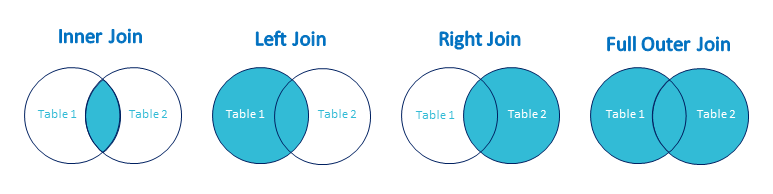
\includegraphics{img/da-dplyr/Joins_Diagram.png}

Joins on table are look like this:

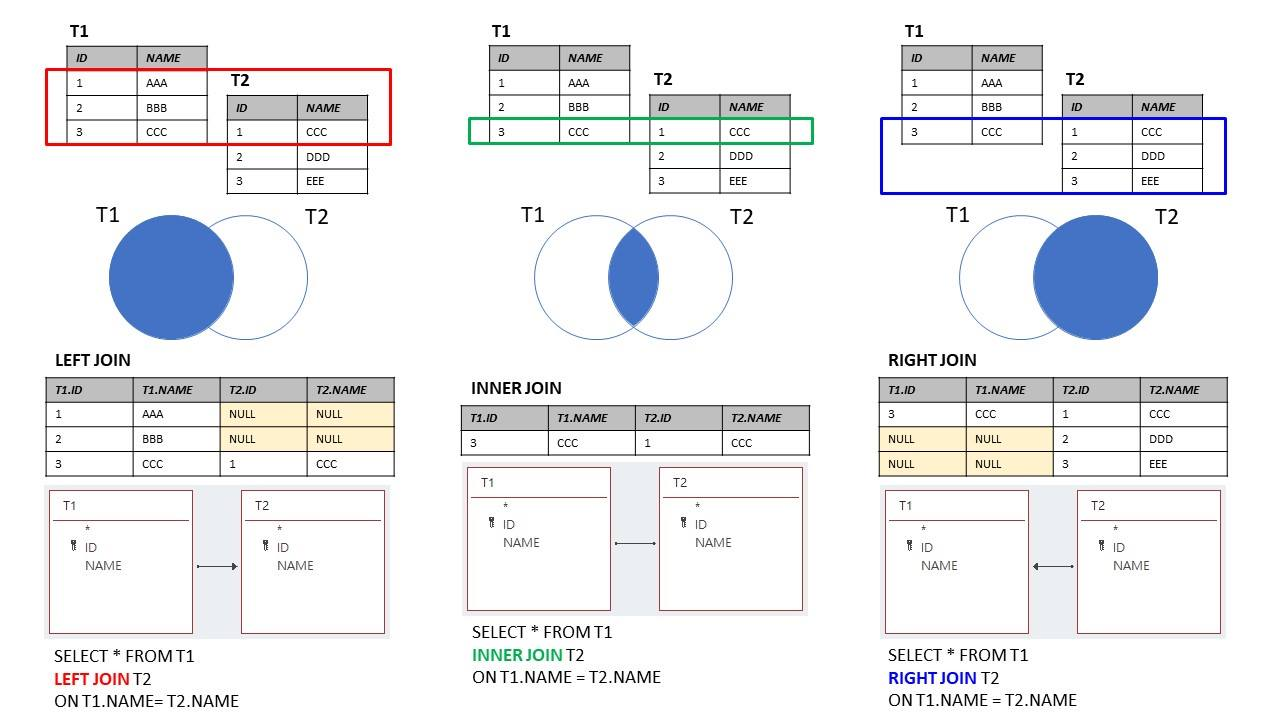
\includegraphics{img/da-dplyr/sqljoin1.jpg}

\begin{center}\rule{0.5\linewidth}{0.5pt}\end{center}

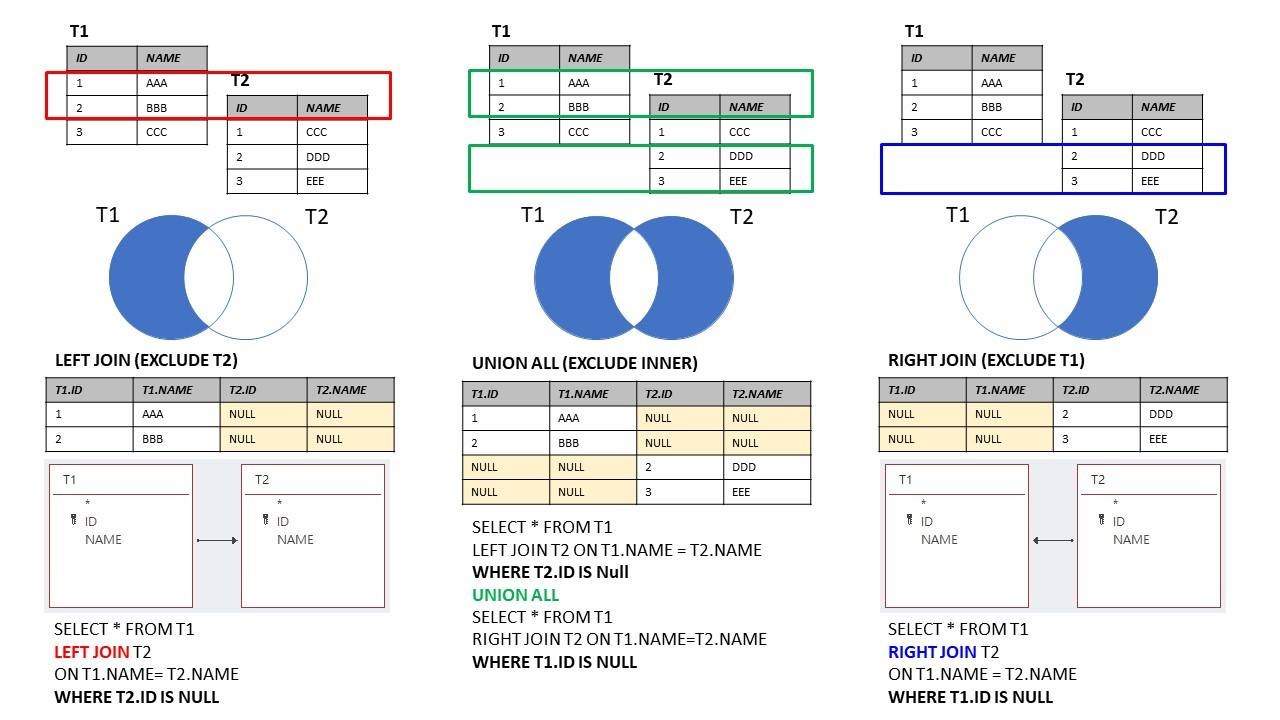
\includegraphics{img/da-dplyr/sqljoin2.jpg}

\begin{center}\rule{0.5\linewidth}{0.5pt}\end{center}

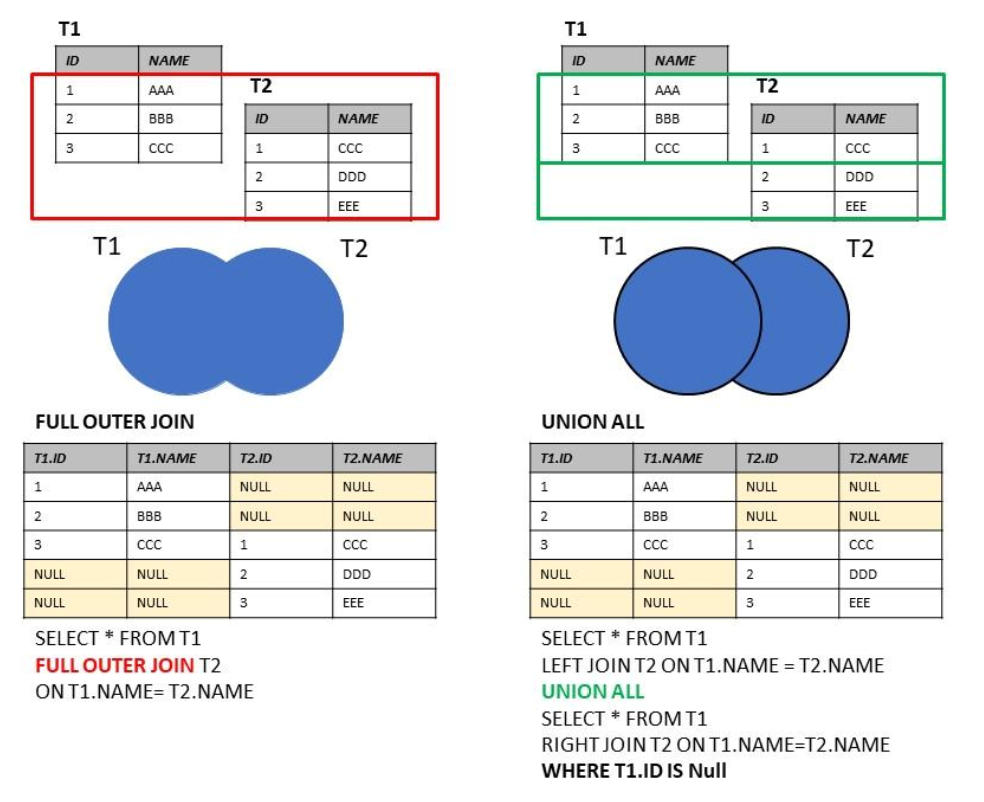
\includegraphics{img/da-dplyr/sqljoin3.png}

Source:
https://marcus116.blogspot.com/2019/07/cheatsheets-sql-join-cheat-sheets.html

\begin{center}\rule{0.5\linewidth}{0.5pt}\end{center}

\section{\texorpdfstring{\texttt{Join}
functions}{Join functions}}\label{join-functions}

To solve previous problem you can use set of \texttt{join()}-functions.
\texttt{left\_join()} can solve our previous example:

\begin{Shaded}
\begin{Highlighting}[]
\NormalTok{d2002 }\OtherTok{\textless{}{-}}\NormalTok{ gapminder }\SpecialCharTok{\%\textgreater{}\%}
            \FunctionTok{filter}\NormalTok{(year }\SpecialCharTok{==} \DecValTok{2002}\NormalTok{) }\SpecialCharTok{\%\textgreater{}\%} \CommentTok{\# year}
            \FunctionTok{group\_by}\NormalTok{(continent, year) }\SpecialCharTok{\%\textgreater{}\%} \CommentTok{\# grouping condition}
            \FunctionTok{summarise}\NormalTok{(}
                \AttributeTok{lifeExpAvg =} \FunctionTok{mean}\NormalTok{(lifeExp),}
                \AttributeTok{countriesCount =} \FunctionTok{n}\NormalTok{(), }\CommentTok{\# n() count of rows in group }
                \AttributeTok{.groups =} \StringTok{\textquotesingle{}drop\textquotesingle{}}
\NormalTok{            )}
\NormalTok{d2002 }\SpecialCharTok{|\textgreater{}} \FunctionTok{head}\NormalTok{()}
\end{Highlighting}
\end{Shaded}

A tibble: 5 × 4

\begin{longtable}[]{@{}
  >{\raggedright\arraybackslash}p{(\columnwidth - 6\tabcolsep) * \real{0.2500}}
  >{\raggedright\arraybackslash}p{(\columnwidth - 6\tabcolsep) * \real{0.2500}}
  >{\raggedright\arraybackslash}p{(\columnwidth - 6\tabcolsep) * \real{0.2500}}
  >{\raggedright\arraybackslash}p{(\columnwidth - 6\tabcolsep) * \real{0.2500}}@{}}
\toprule\noalign{}
\begin{minipage}[b]{\linewidth}\raggedright
continent \textless fct\textgreater{}
\end{minipage} & \begin{minipage}[b]{\linewidth}\raggedright
year \textless int\textgreater{}
\end{minipage} & \begin{minipage}[b]{\linewidth}\raggedright
lifeExpAvg \textless dbl\textgreater{}
\end{minipage} & \begin{minipage}[b]{\linewidth}\raggedright
countriesCount \textless int\textgreater{}
\end{minipage} \\
\midrule\noalign{}
\endhead
\bottomrule\noalign{}
\endlastfoot
Africa & 2002 & 53.32523 & 52 \\
Americas & 2002 & 72.42204 & 25 \\
Asia & 2002 & 69.23388 & 33 \\
Europe & 2002 & 76.70060 & 30 \\
Oceania & 2002 & 79.74000 & 2 \\
\end{longtable}

\begin{Shaded}
\begin{Highlighting}[]
\NormalTok{grouped\_data2002pop }\OtherTok{\textless{}{-}}\NormalTok{ gapminder }\SpecialCharTok{\%\textgreater{}\%}
    \FunctionTok{filter}\NormalTok{(year }\SpecialCharTok{==} \DecValTok{2002}\NormalTok{) }\SpecialCharTok{\%\textgreater{}\%} \CommentTok{\# year}
    \FunctionTok{group\_by}\NormalTok{(continent) }\SpecialCharTok{\%\textgreater{}\%} \CommentTok{\# grouping condition}
    \FunctionTok{summarise}\NormalTok{(}\AttributeTok{totalPop =} \FunctionTok{sum}\NormalTok{(pop),}
             \AttributeTok{year =} \FunctionTok{min}\NormalTok{(year))}

\NormalTok{grouped\_data2002pop }\SpecialCharTok{|\textgreater{}} \FunctionTok{head}\NormalTok{()}
\end{Highlighting}
\end{Shaded}

A tibble: 5 × 3

\begin{longtable}[]{@{}lll@{}}
\toprule\noalign{}
continent \textless fct\textgreater{} & totalPop
\textless dbl\textgreater{} & year \textless int\textgreater{} \\
\midrule\noalign{}
\endhead
\bottomrule\noalign{}
\endlastfoot
Africa & 833723916 & 2002 \\
Americas & 849772762 & 2002 \\
Asia & 3601802203 & 2002 \\
Europe & 578223869 & 2002 \\
Oceania & 23454829 & 2002 \\
\end{longtable}

\begin{Shaded}
\begin{Highlighting}[]
\NormalTok{grouped\_data2002pop }\OtherTok{\textless{}{-}}\NormalTok{ grouped\_data2002pop }\SpecialCharTok{\%\textgreater{}\%} 
    \FunctionTok{arrange}\NormalTok{(totalPop)}

\NormalTok{grouped\_data }\OtherTok{\textless{}{-}}\NormalTok{ d2002 }\SpecialCharTok{\%\textgreater{}\%} 
    \FunctionTok{left\_join}\NormalTok{(grouped\_data2002pop, }\AttributeTok{by =} \StringTok{"continent"}\NormalTok{)}
\NormalTok{grouped\_data}

\CommentTok{\# but we have duplicated year}
\end{Highlighting}
\end{Shaded}

A tibble: 5 × 6

\begin{longtable}[]{@{}
  >{\raggedright\arraybackslash}p{(\columnwidth - 10\tabcolsep) * \real{0.1667}}
  >{\raggedright\arraybackslash}p{(\columnwidth - 10\tabcolsep) * \real{0.1667}}
  >{\raggedright\arraybackslash}p{(\columnwidth - 10\tabcolsep) * \real{0.1667}}
  >{\raggedright\arraybackslash}p{(\columnwidth - 10\tabcolsep) * \real{0.1667}}
  >{\raggedright\arraybackslash}p{(\columnwidth - 10\tabcolsep) * \real{0.1667}}
  >{\raggedright\arraybackslash}p{(\columnwidth - 10\tabcolsep) * \real{0.1667}}@{}}
\toprule\noalign{}
\begin{minipage}[b]{\linewidth}\raggedright
continent \textless fct\textgreater{}
\end{minipage} & \begin{minipage}[b]{\linewidth}\raggedright
year.x \textless int\textgreater{}
\end{minipage} & \begin{minipage}[b]{\linewidth}\raggedright
lifeExpAvg \textless dbl\textgreater{}
\end{minipage} & \begin{minipage}[b]{\linewidth}\raggedright
countriesCount \textless int\textgreater{}
\end{minipage} & \begin{minipage}[b]{\linewidth}\raggedright
totalPop \textless dbl\textgreater{}
\end{minipage} & \begin{minipage}[b]{\linewidth}\raggedright
year.y \textless int\textgreater{}
\end{minipage} \\
\midrule\noalign{}
\endhead
\bottomrule\noalign{}
\endlastfoot
Africa & 2002 & 53.32523 & 52 & 833723916 & 2002 \\
Americas & 2002 & 72.42204 & 25 & 849772762 & 2002 \\
Asia & 2002 & 69.23388 & 33 & 3601802203 & 2002 \\
Europe & 2002 & 76.70060 & 30 & 578223869 & 2002 \\
Oceania & 2002 & 79.74000 & 2 & 23454829 & 2002 \\
\end{longtable}

\begin{Shaded}
\begin{Highlighting}[]
\NormalTok{grouped\_data2002pop }\OtherTok{\textless{}{-}}\NormalTok{ grouped\_data2002pop }\SpecialCharTok{\%\textgreater{}\%} 
    \FunctionTok{arrange}\NormalTok{(totalPop)}

\NormalTok{grouped\_data }\OtherTok{\textless{}{-}}\NormalTok{ d2002 }\SpecialCharTok{\%\textgreater{}\%} 
    \FunctionTok{left\_join}\NormalTok{(grouped\_data2002pop, }\AttributeTok{by =} \FunctionTok{c}\NormalTok{(}\StringTok{"continent"}\NormalTok{, }\StringTok{"year"}\NormalTok{))}
\NormalTok{grouped\_data}

\CommentTok{\#ok}
\end{Highlighting}
\end{Shaded}

A tibble: 5 × 5

\begin{longtable}[]{@{}
  >{\raggedright\arraybackslash}p{(\columnwidth - 8\tabcolsep) * \real{0.2000}}
  >{\raggedright\arraybackslash}p{(\columnwidth - 8\tabcolsep) * \real{0.2000}}
  >{\raggedright\arraybackslash}p{(\columnwidth - 8\tabcolsep) * \real{0.2000}}
  >{\raggedright\arraybackslash}p{(\columnwidth - 8\tabcolsep) * \real{0.2000}}
  >{\raggedright\arraybackslash}p{(\columnwidth - 8\tabcolsep) * \real{0.2000}}@{}}
\toprule\noalign{}
\begin{minipage}[b]{\linewidth}\raggedright
continent \textless fct\textgreater{}
\end{minipage} & \begin{minipage}[b]{\linewidth}\raggedright
year \textless int\textgreater{}
\end{minipage} & \begin{minipage}[b]{\linewidth}\raggedright
lifeExpAvg \textless dbl\textgreater{}
\end{minipage} & \begin{minipage}[b]{\linewidth}\raggedright
countriesCount \textless int\textgreater{}
\end{minipage} & \begin{minipage}[b]{\linewidth}\raggedright
totalPop \textless dbl\textgreater{}
\end{minipage} \\
\midrule\noalign{}
\endhead
\bottomrule\noalign{}
\endlastfoot
Africa & 2002 & 53.32523 & 52 & 833723916 \\
Americas & 2002 & 72.42204 & 25 & 849772762 \\
Asia & 2002 & 69.23388 & 33 & 3601802203 \\
Europe & 2002 & 76.70060 & 30 & 578223869 \\
Oceania & 2002 & 79.74000 & 2 & 23454829 \\
\end{longtable}

Let's make a different data sets for testing \texttt{join()} fucntions:

\begin{Shaded}
\begin{Highlighting}[]
\NormalTok{first\_df }\OtherTok{\textless{}{-}} \FunctionTok{data.frame}\NormalTok{(}\AttributeTok{Letter =} \FunctionTok{c}\NormalTok{(}\StringTok{"A"}\NormalTok{, }\StringTok{"B"}\NormalTok{, }\StringTok{"C"}\NormalTok{, }\StringTok{"D"}\NormalTok{, }\StringTok{"E"}\NormalTok{),}
                      \AttributeTok{Value =} \FunctionTok{c}\NormalTok{(}\DecValTok{1}\SpecialCharTok{:}\DecValTok{5}\NormalTok{))}

\NormalTok{second\_df }\OtherTok{\textless{}{-}} \FunctionTok{data.frame}\NormalTok{(}\AttributeTok{Letter =} \FunctionTok{c}\NormalTok{(}\StringTok{"A"}\NormalTok{, }\StringTok{"B"}\NormalTok{, }\StringTok{"C"}\NormalTok{, }\StringTok{"D"}\NormalTok{, }\StringTok{"F"}\NormalTok{),}
                      \AttributeTok{Value =} \FunctionTok{c}\NormalTok{(}\DecValTok{12}\NormalTok{, }\DecValTok{7}\NormalTok{, }\DecValTok{4}\NormalTok{, }\DecValTok{1}\NormalTok{, }\DecValTok{5}\NormalTok{))}
\NormalTok{first\_df}
\NormalTok{second\_df }
\end{Highlighting}
\end{Shaded}

A data.frame: 5 × 2

\begin{longtable}[]{@{}ll@{}}
\toprule\noalign{}
Letter \textless chr\textgreater{} & Value
\textless int\textgreater{} \\
\midrule\noalign{}
\endhead
\bottomrule\noalign{}
\endlastfoot
A & 1 \\
B & 2 \\
C & 3 \\
D & 4 \\
E & 5 \\
\end{longtable}

A data.frame: 5 × 2

\begin{longtable}[]{@{}ll@{}}
\toprule\noalign{}
Letter \textless chr\textgreater{} & Value
\textless dbl\textgreater{} \\
\midrule\noalign{}
\endhead
\bottomrule\noalign{}
\endlastfoot
A & 12 \\
B & 7 \\
C & 4 \\
D & 1 \\
F & 5 \\
\end{longtable}

You can see that the last row \texttt{Letter} is different in
dataframes. \texttt{left\_join()} test is next.

\begin{Shaded}
\begin{Highlighting}[]
\NormalTok{first\_df }\SpecialCharTok{\%\textgreater{}\%} 
    \FunctionTok{left\_join}\NormalTok{(second\_df, }\AttributeTok{by =} \StringTok{"Letter"}\NormalTok{)}
\CommentTok{\# there is no F letter, becouse first\_db joined only known first\_df Letters.}
\end{Highlighting}
\end{Shaded}

A data.frame: 5 × 3

\begin{longtable}[]{@{}lll@{}}
\toprule\noalign{}
Letter \textless chr\textgreater{} & Value.x \textless int\textgreater{}
& Value.y \textless dbl\textgreater{} \\
\midrule\noalign{}
\endhead
\bottomrule\noalign{}
\endlastfoot
A & 1 & 12 \\
B & 2 & 7 \\
C & 3 & 4 \\
D & 4 & 1 \\
E & 5 & NA \\
\end{longtable}

\begin{Shaded}
\begin{Highlighting}[]
\NormalTok{first\_df }\SpecialCharTok{\%\textgreater{}\%} 
    \FunctionTok{right\_join}\NormalTok{(second\_df, }\AttributeTok{by =} \StringTok{"Letter"}\NormalTok{)}
\CommentTok{\# right\_join! there is no E letter, becouse first\_db joined only known second\_df Letters.}
\end{Highlighting}
\end{Shaded}

A data.frame: 5 × 3

\begin{longtable}[]{@{}lll@{}}
\toprule\noalign{}
Letter \textless chr\textgreater{} & Value.x \textless int\textgreater{}
& Value.y \textless dbl\textgreater{} \\
\midrule\noalign{}
\endhead
\bottomrule\noalign{}
\endlastfoot
A & 1 & 12 \\
B & 2 & 7 \\
C & 3 & 4 \\
D & 4 & 1 \\
F & NA & 5 \\
\end{longtable}

\begin{Shaded}
\begin{Highlighting}[]
\NormalTok{first\_df }\SpecialCharTok{\%\textgreater{}\%} 
    \FunctionTok{inner\_join}\NormalTok{(second\_df, }\AttributeTok{by =} \StringTok{"Letter"}\NormalTok{)}
\CommentTok{\# inner\_join! there is no E and F Letters, }
\CommentTok{\# only known both first\_df and second\_df are left here.}
\end{Highlighting}
\end{Shaded}

A data.frame: 4 × 3

\begin{longtable}[]{@{}lll@{}}
\toprule\noalign{}
Letter \textless chr\textgreater{} & Value.x \textless int\textgreater{}
& Value.y \textless dbl\textgreater{} \\
\midrule\noalign{}
\endhead
\bottomrule\noalign{}
\endlastfoot
A & 1 & 12 \\
B & 2 & 7 \\
C & 3 & 4 \\
D & 4 & 1 \\
\end{longtable}

\begin{Shaded}
\begin{Highlighting}[]
\NormalTok{first\_df }\SpecialCharTok{\%\textgreater{}\%} 
    \FunctionTok{full\_join}\NormalTok{(second\_df, }\AttributeTok{by =} \StringTok{"Letter"}\NormalTok{)}
\CommentTok{\# all are here, but unknown values replaced by NA, it\textquotesingle{}s ok.}
\end{Highlighting}
\end{Shaded}

A data.frame: 6 × 3

\begin{longtable}[]{@{}lll@{}}
\toprule\noalign{}
Letter \textless chr\textgreater{} & Value.x \textless int\textgreater{}
& Value.y \textless dbl\textgreater{} \\
\midrule\noalign{}
\endhead
\bottomrule\noalign{}
\endlastfoot
A & 1 & 12 \\
B & 2 & 7 \\
C & 3 & 4 \\
D & 4 & 1 \\
E & 5 & NA \\
F & NA & 5 \\
\end{longtable}

Short description of reviewed functions:

\begin{longtable}[]{@{}
  >{\raggedright\arraybackslash}p{(\columnwidth - 6\tabcolsep) * \real{0.2500}}
  >{\raggedright\arraybackslash}p{(\columnwidth - 6\tabcolsep) * \real{0.2500}}
  >{\raggedright\arraybackslash}p{(\columnwidth - 6\tabcolsep) * \real{0.2500}}
  >{\raggedright\arraybackslash}p{(\columnwidth - 6\tabcolsep) * \real{0.2500}}@{}}
\toprule\noalign{}
\begin{minipage}[b]{\linewidth}\raggedright
Function
\end{minipage} & \begin{minipage}[b]{\linewidth}\raggedright
Objectives
\end{minipage} & \begin{minipage}[b]{\linewidth}\raggedright
Arguments
\end{minipage} & \begin{minipage}[b]{\linewidth}\raggedright
Multiple keys
\end{minipage} \\
\midrule\noalign{}
\endhead
\bottomrule\noalign{}
\endlastfoot
\texttt{left\_join()} & Merge two datasets. Keep all observations from
the origin table & data, origin, destination, by = ``ID'' & origin,
destination, by = c(``ID'', ``ID2'') \\
\texttt{right\_join()} & Merge two datasets. Keep all observations from
the destination table & data, origin, destination, by = ``ID'' & origin,
destination, by = c(``ID'', ``ID2'') \\
\texttt{inner\_join()} & Merge two datasets. Excludes all unmatched rows
& data, origin, destination, by = ``ID'' & origin, destination, by =
c(``ID'', ``ID2'') \\
\texttt{full\_join()} & Merge two datasets. Keeps all observations &
data, origin, destination, by = ``ID'' & origin, destination, by =
c(``ID'', ``ID2'') \\
\end{longtable}

\begin{center}\rule{0.5\linewidth}{0.5pt}\end{center}

\section{Refences}\label{refences-8}

\begin{enumerate}
\def\labelenumi{\arabic{enumi}.}
\tightlist
\item
  \href{https://cran.r-project.org/web/packages/dplyr/index.html}{dplyr:
  A Grammar of Data Manipulation} on https://cran.r-project.org/.
\item
  \href{https://github.com/rstudio/cheatsheets/blob/master/data-transformation.pdf}{Data
  Transformation with splyr::cheat sheet}.
\item
  \href{https://www.listendata.com/2016/08/dplyr-tutorial.html}{DPLYR
  TUTORIAL : DATA MANIPULATION (50 EXAMPLES)} by Deepanshu Bhalla.
\item
  \href{https://stat545.com/dplyr-intro.html}{Dplyr Intro} by Stat 545.
  6.\href{https://www.guru99.com/r-dplyr-tutorial.html}{R Dplyr
  Tutorial: Data Manipulation(Join) \& Cleaning(Spread)}. Introduction
  to Data Analysis
\item
  \href{https://www.kaggle.com/kmldas/loan-default-prediction}{Loan
  Default Prediction. Beginners data set for financial analytics Kaggle}
\end{enumerate}

\chapter{Wide-to-long tables}\label{wide-to-long-tables}

\begin{center}\rule{0.5\linewidth}{0.5pt}\end{center}

author: Юрій Клебан

\begin{center}\rule{0.5\linewidth}{0.5pt}\end{center}

Before start load packages

\begin{Shaded}
\begin{Highlighting}[]
\FunctionTok{library}\NormalTok{(tidyr)}
\end{Highlighting}
\end{Shaded}

Some times your data is not in tidy format. Peole can collect data year
by year in each column. It's problem to use such data for feature
engeniering and building prediction models. Let's generate such data
sample (quaterly salary of some people).

\begin{Shaded}
\begin{Highlighting}[]
\NormalTok{not\_good\_data }\OtherTok{\textless{}{-}} \FunctionTok{data.frame}\NormalTok{(}\AttributeTok{Name =} \FunctionTok{c}\NormalTok{(}\StringTok{"Nick"}\NormalTok{, }\StringTok{"Jake"}\NormalTok{, }\StringTok{"Anna"}\NormalTok{, }\StringTok{"Jane"}\NormalTok{, }\StringTok{"Dina"}\NormalTok{),}
                           \AttributeTok{q1\_2021 =} \FunctionTok{c}\NormalTok{(}\DecValTok{12442}\NormalTok{, }\DecValTok{22131}\NormalTok{, }\DecValTok{21343}\NormalTok{, }\DecValTok{22111}\NormalTok{, }\DecValTok{14123}\NormalTok{),}
                           \AttributeTok{q2\_2021 =} \FunctionTok{c}\NormalTok{(}\DecValTok{13442}\NormalTok{, }\DecValTok{22871}\NormalTok{, }\DecValTok{20343}\NormalTok{, }\DecValTok{22222}\NormalTok{, }\DecValTok{14456}\NormalTok{),}
                           \AttributeTok{q3\_2021 =} \FunctionTok{c}\NormalTok{(}\DecValTok{15482}\NormalTok{, }\DecValTok{22031}\NormalTok{, }\DecValTok{22456}\NormalTok{, }\DecValTok{22444}\NormalTok{, }\DecValTok{14533}\NormalTok{),}
                           \AttributeTok{q4\_2021 =} \FunctionTok{c}\NormalTok{(}\DecValTok{14511}\NormalTok{, }\DecValTok{20031}\NormalTok{, }\DecValTok{21741}\NormalTok{, }\DecValTok{22333}\NormalTok{, }\DecValTok{14511}\NormalTok{))}
\NormalTok{not\_good\_data}
\end{Highlighting}
\end{Shaded}

A data.frame: 5 × 5

\begin{longtable}[]{@{}
  >{\raggedright\arraybackslash}p{(\columnwidth - 8\tabcolsep) * \real{0.2000}}
  >{\raggedright\arraybackslash}p{(\columnwidth - 8\tabcolsep) * \real{0.2000}}
  >{\raggedright\arraybackslash}p{(\columnwidth - 8\tabcolsep) * \real{0.2000}}
  >{\raggedright\arraybackslash}p{(\columnwidth - 8\tabcolsep) * \real{0.2000}}
  >{\raggedright\arraybackslash}p{(\columnwidth - 8\tabcolsep) * \real{0.2000}}@{}}
\toprule\noalign{}
\begin{minipage}[b]{\linewidth}\raggedright
Name \textless chr\textgreater{}
\end{minipage} & \begin{minipage}[b]{\linewidth}\raggedright
q1\_2021 \textless dbl\textgreater{}
\end{minipage} & \begin{minipage}[b]{\linewidth}\raggedright
q2\_2021 \textless dbl\textgreater{}
\end{minipage} & \begin{minipage}[b]{\linewidth}\raggedright
q3\_2021 \textless dbl\textgreater{}
\end{minipage} & \begin{minipage}[b]{\linewidth}\raggedright
q4\_2021 \textless dbl\textgreater{}
\end{minipage} \\
\midrule\noalign{}
\endhead
\bottomrule\noalign{}
\endlastfoot
Nick & 12442 & 13442 & 15482 & 14511 \\
Jake & 22131 & 22871 & 22031 & 20031 \\
Anna & 21343 & 20343 & 22456 & 21741 \\
Jane & 22111 & 22222 & 22444 & 22333 \\
Dina & 14123 & 14456 & 14533 & 14511 \\
\end{longtable}

\begin{Shaded}
\begin{Highlighting}[]
\NormalTok{better\_data }\OtherTok{\textless{}{-}}\NormalTok{ not\_good\_data }\SpecialCharTok{\%\textgreater{}\%}
                \FunctionTok{gather}\NormalTok{(quater, salary, }\DecValTok{2}\SpecialCharTok{:}\DecValTok{5}\NormalTok{)}
                \CommentTok{\# gather(quater, salary, q1\_2021:q4\_2021) possible code too}
\NormalTok{better\_data}
\end{Highlighting}
\end{Shaded}

A data.frame: 20 × 3

\begin{longtable}[]{@{}lll@{}}
\toprule\noalign{}
Name \textless chr\textgreater{} & quater \textless chr\textgreater{} &
salary \textless dbl\textgreater{} \\
\midrule\noalign{}
\endhead
\bottomrule\noalign{}
\endlastfoot
Nick & q1\_2021 & 12442 \\
Jake & q1\_2021 & 22131 \\
Anna & q1\_2021 & 21343 \\
Jane & q1\_2021 & 22111 \\
Dina & q1\_2021 & 14123 \\
Nick & q2\_2021 & 13442 \\
Jake & q2\_2021 & 22871 \\
Anna & q2\_2021 & 20343 \\
Jane & q2\_2021 & 22222 \\
Dina & q2\_2021 & 14456 \\
Nick & q3\_2021 & 15482 \\
Jake & q3\_2021 & 22031 \\
Anna & q3\_2021 & 22456 \\
Jane & q3\_2021 & 22444 \\
Dina & q3\_2021 & 14533 \\
Nick & q4\_2021 & 14511 \\
Jake & q4\_2021 & 20031 \\
Anna & q4\_2021 & 21741 \\
Jane & q4\_2021 & 22333 \\
Dina & q4\_2021 & 14511 \\
\end{longtable}

To make our data tidier \texttt{separate()} can split quater column into
2 (\texttt{quater} and \texttt{year}):

\begin{Shaded}
\begin{Highlighting}[]
\NormalTok{best\_data }\OtherTok{\textless{}{-}}\NormalTok{ better\_data }\SpecialCharTok{\%\textgreater{}\%}
    \FunctionTok{separate}\NormalTok{(quater, }\FunctionTok{c}\NormalTok{(}\StringTok{"quater"}\NormalTok{, }\StringTok{"year"}\NormalTok{), }\AttributeTok{sep =} \StringTok{"\_"}\NormalTok{) }\SpecialCharTok{\%\textgreater{}\%} \CommentTok{\# separate}
    \FunctionTok{mutate}\NormalTok{(}\AttributeTok{year =} \FunctionTok{as.integer}\NormalTok{(year), }\CommentTok{\# convert year to integer}
           \AttributeTok{quater =} \FunctionTok{substr}\NormalTok{(better\_data}\SpecialCharTok{$}\NormalTok{quater, }\DecValTok{2}\NormalTok{,}\DecValTok{2}\NormalTok{), }\CommentTok{\# trim \textasciigrave{}q\textasciigrave{} from start}
           \AttributeTok{quater =} \FunctionTok{as.integer}\NormalTok{(quater), }\CommentTok{\# convert quater to integer}
\NormalTok{          ) }\SpecialCharTok{\%\textgreater{}\%}
    \FunctionTok{head}\NormalTok{(}\DecValTok{10}\NormalTok{)}
\NormalTok{best\_data}
\end{Highlighting}
\end{Shaded}

A data.frame: 10 × 4

\begin{longtable}[]{@{}
  >{\raggedright\arraybackslash}p{(\columnwidth - 8\tabcolsep) * \real{0.2000}}
  >{\raggedright\arraybackslash}p{(\columnwidth - 8\tabcolsep) * \real{0.2000}}
  >{\raggedright\arraybackslash}p{(\columnwidth - 8\tabcolsep) * \real{0.2000}}
  >{\raggedright\arraybackslash}p{(\columnwidth - 8\tabcolsep) * \real{0.2000}}
  >{\raggedright\arraybackslash}p{(\columnwidth - 8\tabcolsep) * \real{0.2000}}@{}}
\toprule\noalign{}
\begin{minipage}[b]{\linewidth}\raggedright
\end{minipage} & \begin{minipage}[b]{\linewidth}\raggedright
Name \textless chr\textgreater{}
\end{minipage} & \begin{minipage}[b]{\linewidth}\raggedright
quater \textless int\textgreater{}
\end{minipage} & \begin{minipage}[b]{\linewidth}\raggedright
year \textless int\textgreater{}
\end{minipage} & \begin{minipage}[b]{\linewidth}\raggedright
salary \textless dbl\textgreater{}
\end{minipage} \\
\midrule\noalign{}
\endhead
\bottomrule\noalign{}
\endlastfoot
1 & Nick & 1 & 2021 & 12442 \\
2 & Jake & 1 & 2021 & 22131 \\
3 & Anna & 1 & 2021 & 21343 \\
4 & Jane & 1 & 2021 & 22111 \\
5 & Dina & 1 & 2021 & 14123 \\
6 & Nick & 2 & 2021 & 13442 \\
7 & Jake & 2 & 2021 & 22871 \\
8 & Anna & 2 & 2021 & 20343 \\
9 & Jane & 2 & 2021 & 22222 \\
10 & Dina & 2 & 2021 & 14456 \\
\end{longtable}

The \texttt{unite()} function concanates two columns into one:

\begin{Shaded}
\begin{Highlighting}[]
\NormalTok{united\_data }\OtherTok{\textless{}{-}}\NormalTok{ best\_data }\SpecialCharTok{\%\textgreater{}\%}
                \FunctionTok{unite}\NormalTok{(Qt, quater, year, }\AttributeTok{sep =} \StringTok{"\#"}\NormalTok{)}
\NormalTok{united\_data}
\end{Highlighting}
\end{Shaded}

A data.frame: 10 × 3

\begin{longtable}[]{@{}llll@{}}
\toprule\noalign{}
& Name \textless chr\textgreater{} & Qt \textless chr\textgreater{} &
salary \textless dbl\textgreater{} \\
\midrule\noalign{}
\endhead
\bottomrule\noalign{}
\endlastfoot
1 & Nick & 1\#2021 & 12442 \\
2 & Jake & 1\#2021 & 22131 \\
3 & Anna & 1\#2021 & 21343 \\
4 & Jane & 1\#2021 & 22111 \\
5 & Dina & 1\#2021 & 14123 \\
6 & Nick & 2\#2021 & 13442 \\
7 & Jake & 2\#2021 & 22871 \\
8 & Anna & 2\#2021 & 20343 \\
9 & Jane & 2\#2021 & 22222 \\
10 & Dina & 2\#2021 & 14456 \\
\end{longtable}

\begin{Shaded}
\begin{Highlighting}[]
\CommentTok{\# if dont want remove old columns use remove param}
\NormalTok{united\_data }\OtherTok{\textless{}{-}}\NormalTok{ best\_data }\SpecialCharTok{\%\textgreater{}\%}
                \FunctionTok{unite}\NormalTok{(Qt, quater, year, }\AttributeTok{sep =} \StringTok{"\#"}\NormalTok{, }\AttributeTok{remove =}\NormalTok{ F)}
\NormalTok{united\_data}
\end{Highlighting}
\end{Shaded}

A data.frame: 10 × 5

\begin{longtable}[]{@{}
  >{\raggedright\arraybackslash}p{(\columnwidth - 10\tabcolsep) * \real{0.1667}}
  >{\raggedright\arraybackslash}p{(\columnwidth - 10\tabcolsep) * \real{0.1667}}
  >{\raggedright\arraybackslash}p{(\columnwidth - 10\tabcolsep) * \real{0.1667}}
  >{\raggedright\arraybackslash}p{(\columnwidth - 10\tabcolsep) * \real{0.1667}}
  >{\raggedright\arraybackslash}p{(\columnwidth - 10\tabcolsep) * \real{0.1667}}
  >{\raggedright\arraybackslash}p{(\columnwidth - 10\tabcolsep) * \real{0.1667}}@{}}
\toprule\noalign{}
\begin{minipage}[b]{\linewidth}\raggedright
\end{minipage} & \begin{minipage}[b]{\linewidth}\raggedright
Name \textless chr\textgreater{}
\end{minipage} & \begin{minipage}[b]{\linewidth}\raggedright
Qt \textless chr\textgreater{}
\end{minipage} & \begin{minipage}[b]{\linewidth}\raggedright
quater \textless int\textgreater{}
\end{minipage} & \begin{minipage}[b]{\linewidth}\raggedright
year \textless int\textgreater{}
\end{minipage} & \begin{minipage}[b]{\linewidth}\raggedright
salary \textless dbl\textgreater{}
\end{minipage} \\
\midrule\noalign{}
\endhead
\bottomrule\noalign{}
\endlastfoot
1 & Nick & 1\#2021 & 1 & 2021 & 12442 \\
2 & Jake & 1\#2021 & 1 & 2021 & 22131 \\
3 & Anna & 1\#2021 & 1 & 2021 & 21343 \\
4 & Jane & 1\#2021 & 1 & 2021 & 22111 \\
5 & Dina & 1\#2021 & 1 & 2021 & 14123 \\
6 & Nick & 2\#2021 & 2 & 2021 & 13442 \\
7 & Jake & 2\#2021 & 2 & 2021 & 22871 \\
8 & Anna & 2\#2021 & 2 & 2021 & 20343 \\
9 & Jane & 2\#2021 & 2 & 2021 & 22222 \\
10 & Dina & 2\#2021 & 2 & 2021 & 14456 \\
\end{longtable}

If you need to make table like initial use \texttt{spread()} function:

\begin{Shaded}
\begin{Highlighting}[]
\NormalTok{not\_good\_data2 }\OtherTok{\textless{}{-}}\NormalTok{ better\_data }\SpecialCharTok{\%\textgreater{}\%}
                    \FunctionTok{spread}\NormalTok{(quater, salary)}
\NormalTok{not\_good\_data2}
\end{Highlighting}
\end{Shaded}

A data.frame: 5 × 5

\begin{longtable}[]{@{}
  >{\raggedright\arraybackslash}p{(\columnwidth - 8\tabcolsep) * \real{0.2000}}
  >{\raggedright\arraybackslash}p{(\columnwidth - 8\tabcolsep) * \real{0.2000}}
  >{\raggedright\arraybackslash}p{(\columnwidth - 8\tabcolsep) * \real{0.2000}}
  >{\raggedright\arraybackslash}p{(\columnwidth - 8\tabcolsep) * \real{0.2000}}
  >{\raggedright\arraybackslash}p{(\columnwidth - 8\tabcolsep) * \real{0.2000}}@{}}
\toprule\noalign{}
\begin{minipage}[b]{\linewidth}\raggedright
Name \textless chr\textgreater{}
\end{minipage} & \begin{minipage}[b]{\linewidth}\raggedright
q1\_2021 \textless dbl\textgreater{}
\end{minipage} & \begin{minipage}[b]{\linewidth}\raggedright
q2\_2021 \textless dbl\textgreater{}
\end{minipage} & \begin{minipage}[b]{\linewidth}\raggedright
q3\_2021 \textless dbl\textgreater{}
\end{minipage} & \begin{minipage}[b]{\linewidth}\raggedright
q4\_2021 \textless dbl\textgreater{}
\end{minipage} \\
\midrule\noalign{}
\endhead
\bottomrule\noalign{}
\endlastfoot
Anna & 21343 & 20343 & 22456 & 21741 \\
Dina & 14123 & 14456 & 14533 & 14511 \\
Jake & 22131 & 22871 & 22031 & 20031 \\
Jane & 22111 & 22222 & 22444 & 22333 \\
Nick & 12442 & 13442 & 15482 & 14511 \\
\end{longtable}

Let's try to \texttt{spread()} feild \texttt{pop} of \texttt{gapminder}
by year:

\begin{Shaded}
\begin{Highlighting}[]
\FunctionTok{library}\NormalTok{(gapminder)}
\end{Highlighting}
\end{Shaded}

\begin{Shaded}
\begin{Highlighting}[]
\NormalTok{gapminder }\SpecialCharTok{\%\textgreater{}\%} \FunctionTok{select}\NormalTok{(country, pop, year) }\SpecialCharTok{\%\textgreater{}\%}
                \FunctionTok{spread}\NormalTok{(year, pop) }\SpecialCharTok{\%\textgreater{}\%}
                \FunctionTok{head}\NormalTok{() }\CommentTok{\# for shorter code}

\CommentTok{\# now you can easy send data to your director in excel :)}
\end{Highlighting}
\end{Shaded}

A tibble: 6 × 13

\begin{longtable}[]{@{}
  >{\raggedright\arraybackslash}p{(\columnwidth - 24\tabcolsep) * \real{0.0769}}
  >{\raggedright\arraybackslash}p{(\columnwidth - 24\tabcolsep) * \real{0.0769}}
  >{\raggedright\arraybackslash}p{(\columnwidth - 24\tabcolsep) * \real{0.0769}}
  >{\raggedright\arraybackslash}p{(\columnwidth - 24\tabcolsep) * \real{0.0769}}
  >{\raggedright\arraybackslash}p{(\columnwidth - 24\tabcolsep) * \real{0.0769}}
  >{\raggedright\arraybackslash}p{(\columnwidth - 24\tabcolsep) * \real{0.0769}}
  >{\raggedright\arraybackslash}p{(\columnwidth - 24\tabcolsep) * \real{0.0769}}
  >{\raggedright\arraybackslash}p{(\columnwidth - 24\tabcolsep) * \real{0.0769}}
  >{\raggedright\arraybackslash}p{(\columnwidth - 24\tabcolsep) * \real{0.0769}}
  >{\raggedright\arraybackslash}p{(\columnwidth - 24\tabcolsep) * \real{0.0769}}
  >{\raggedright\arraybackslash}p{(\columnwidth - 24\tabcolsep) * \real{0.0769}}
  >{\raggedright\arraybackslash}p{(\columnwidth - 24\tabcolsep) * \real{0.0769}}
  >{\raggedright\arraybackslash}p{(\columnwidth - 24\tabcolsep) * \real{0.0769}}@{}}
\toprule\noalign{}
\begin{minipage}[b]{\linewidth}\raggedright
country \textless fct\textgreater{}
\end{minipage} & \begin{minipage}[b]{\linewidth}\raggedright
1952 \textless int\textgreater{}
\end{minipage} & \begin{minipage}[b]{\linewidth}\raggedright
1957 \textless int\textgreater{}
\end{minipage} & \begin{minipage}[b]{\linewidth}\raggedright
1962 \textless int\textgreater{}
\end{minipage} & \begin{minipage}[b]{\linewidth}\raggedright
1967 \textless int\textgreater{}
\end{minipage} & \begin{minipage}[b]{\linewidth}\raggedright
1972 \textless int\textgreater{}
\end{minipage} & \begin{minipage}[b]{\linewidth}\raggedright
1977 \textless int\textgreater{}
\end{minipage} & \begin{minipage}[b]{\linewidth}\raggedright
1982 \textless int\textgreater{}
\end{minipage} & \begin{minipage}[b]{\linewidth}\raggedright
1987 \textless int\textgreater{}
\end{minipage} & \begin{minipage}[b]{\linewidth}\raggedright
1992 \textless int\textgreater{}
\end{minipage} & \begin{minipage}[b]{\linewidth}\raggedright
1997 \textless int\textgreater{}
\end{minipage} & \begin{minipage}[b]{\linewidth}\raggedright
2002 \textless int\textgreater{}
\end{minipage} & \begin{minipage}[b]{\linewidth}\raggedright
2007 \textless int\textgreater{}
\end{minipage} \\
\midrule\noalign{}
\endhead
\bottomrule\noalign{}
\endlastfoot
Afghanistan & 8425333 & 9240934 & 10267083 & 11537966 & 13079460 &
14880372 & 12881816 & 13867957 & 16317921 & 22227415 & 25268405 &
31889923 \\
Albania & 1282697 & 1476505 & 1728137 & 1984060 & 2263554 & 2509048 &
2780097 & 3075321 & 3326498 & 3428038 & 3508512 & 3600523 \\
Algeria & 9279525 & 10270856 & 11000948 & 12760499 & 14760787 & 17152804
& 20033753 & 23254956 & 26298373 & 29072015 & 31287142 & 33333216 \\
Angola & 4232095 & 4561361 & 4826015 & 5247469 & 5894858 & 6162675 &
7016384 & 7874230 & 8735988 & 9875024 & 10866106 & 12420476 \\
Argentina & 17876956 & 19610538 & 21283783 & 22934225 & 24779799 &
26983828 & 29341374 & 31620918 & 33958947 & 36203463 & 38331121 &
40301927 \\
Australia & 8691212 & 9712569 & 10794968 & 11872264 & 13177000 &
14074100 & 15184200 & 16257249 & 17481977 & 18565243 & 19546792 &
20434176 \\
\end{longtable}

Functions table:

\begin{longtable}[]{@{}
  >{\raggedright\arraybackslash}p{(\columnwidth - 4\tabcolsep) * \real{0.3333}}
  >{\raggedright\arraybackslash}p{(\columnwidth - 4\tabcolsep) * \real{0.3333}}
  >{\raggedright\arraybackslash}p{(\columnwidth - 4\tabcolsep) * \real{0.3333}}@{}}
\toprule\noalign{}
\begin{minipage}[b]{\linewidth}\raggedright
Function
\end{minipage} & \begin{minipage}[b]{\linewidth}\raggedright
Objectives
\end{minipage} & \begin{minipage}[b]{\linewidth}\raggedright
Arguments
\end{minipage} \\
\midrule\noalign{}
\endhead
\bottomrule\noalign{}
\endlastfoot
\texttt{gather()} & Transform the data from wide to long & (data, key,
value, na.rm = FALSE) \\
\texttt{spread()} & Transform the data from long to wide & (data, key,
value) \\
\texttt{separate()} & Split one variables into two & (data, col, into,
sep= ``\,``, remove = TRUE) \\
\texttt{unite()} & Unite two variables into one & (data, col, conc ,sep=
``\,``, remove = TRUE) \\
\end{longtable}

\begin{center}\rule{0.5\linewidth}{0.5pt}\end{center}

\section{Refences}\label{refences-9}

\begin{enumerate}
\def\labelenumi{\arabic{enumi}.}
\tightlist
\item
  \href{https://cran.r-project.org/web/packages/dplyr/index.html}{dplyr:
  A Grammar of Data Manipulation} on https://cran.r-project.org/.
\item
  \href{https://github.com/rstudio/cheatsheets/blob/master/data-transformation.pdf}{Data
  Transformation with splyr::cheat sheet}.
\item
  \href{https://www.listendata.com/2016/08/dplyr-tutorial.html}{DPLYR
  TUTORIAL : DATA MANIPULATION (50 EXAMPLES)} by Deepanshu Bhalla.
\item
  \href{https://stat545.com/dplyr-intro.html}{Dplyr Intro} by Stat 545.
  6.\href{https://www.guru99.com/r-dplyr-tutorial.html}{R Dplyr
  Tutorial: Data Manipulation(Join) \& Cleaning(Spread)}. Introduction
  to Data Analysis
\item
  \href{https://www.kaggle.com/kmldas/loan-default-prediction}{Loan
  Default Prediction. Beginners data set for financial analytics Kaggle}
\end{enumerate}

\part{ТЕМА 4. СПОСОБИ ОЧИСТКИ ДАНИХ}

\chapter{Оцінки якості
даних}\label{ux43eux446ux456ux43dux43aux438-ux44fux43aux43eux441ux442ux456-ux434ux430ux43dux438ux445}

\begin{center}\rule{0.5\linewidth}{0.5pt}\end{center}

author: Юрій Клебан

\begin{center}\rule{0.5\linewidth}{0.5pt}\end{center}

Матеріали розділу описують інформацію про виміри оцінки якості даних,
підходи до визначення та обробки пропущених значень, а також
розглядаються способи боротьби зі статистичними викидами.

\section{Що таке валідація
даних?}\label{ux449ux43e-ux442ux430ux43aux435-ux432ux430ux43bux456ux434ux430ux446ux456ux44f-ux434ux430ux43dux438ux445}

Валідація даних відноситься до процесу забезпечення точності та якості
даних. Він реалізується шляхом вбудовування кількох перевірок у систему
або звітування для забезпечення логічної узгодженості введених і
збережених даних.

\begin{center}\rule{0.5\linewidth}{0.5pt}\end{center}

Якість даних залежить від очищення та коригування даних, які відсутні,
некоректні, недійсні або нечитабельні. Для забезпечення достовірності
даних важливо зрозуміти ключові аспекти якості даних, щоб оцінити,
наскільки дані погані/хороші.

На перший погляд, очевидно, що перетворення даних до якісних полягає в
очищенні поганих даних -- даних, які відсутні, неправильні або якимось
чином недійсні. Але щоб переконатися, що дані заслуговують довіри,
важливо розуміти ключові виміри якості даних, щоб оцінити, наскільки
дані є «поганими».

Окремі компанії мають внутрішні документи, що визначають виміри оцінки
якості даних та порядок його проведення -
\texttt{Data\ Validation\ Framework} або
\texttt{Data\ Quality\ Framework}.

Коли говорять про якість даних, то мається на увазі їх оцінка у кількох
вимірах. Розглянемо коротко ці виміри:

\begin{itemize}
\tightlist
\item[$\boxtimes$]
  Правильність / \texttt{Accuracy}
\item[$\boxtimes$]
  Повнота / \texttt{Completeness}
\item[$\boxtimes$]
  Узгодженість / \texttt{Consistency}
\item[$\boxtimes$]
  Відповідність / \texttt{Conformity}
\item[$\boxtimes$]
  Цілісність / \texttt{Integrity}
\item[$\boxtimes$]
  Своєчасність / \texttt{Timeliness}
\item[$\boxtimes$]
  Унікальність / \texttt{Uniqueness}
\end{itemize}

\begin{center}\rule{0.5\linewidth}{0.5pt}\end{center}

\section{Правильність /
(Accuracy)}\label{ux43fux440ux430ux432ux438ux43bux44cux43dux456ux441ux442ux44c-accuracy}

\textbf{Правильність} --- це ступінь, до якого дані правильно
відображають реальний об'єкт АБО описувану подію.

Приклади: - {[}x{]} Реальною вартістю є ціна продажу одиниці товару. -
{[}x{]} Адреса співробітника в \texttt{базі\ даних\ співробітників} є
справжньою адресою.

Запитання, які ви можете задати собі:

\begin{itemize}
\tightlist
\item[$\boxtimes$]
  Чи об'єкти даних точно представляють значення «реального світу», які
  вони повинні моделювати? \emph{Наприклад, чи правильно вказувати вік у
  сотнях тисяч років?}
\item[$\boxtimes$]
  Чи присутнє неправильне написання назв товарів чи осіб, адрес і навіть
  несвоєчасних чи неактуальних даних?
\end{itemize}

Ці проблеми можуть вплинути на результатати аналітичних звітів,
наприклад, неправильні середні значення певних показників.

\begin{center}\rule{0.5\linewidth}{0.5pt}\end{center}

\section{Повнота /
(Completeness)}\label{ux43fux43eux432ux43dux43eux442ux430-completeness}

Повнота визначається як очікувана всебічність. Дані можуть бути повними,
навіть якщо додаткові дані відсутні. Поки дані відповідають очікуванням,
вони вважаються повними.

Наприклад, ім'я та прізвище замовника є обов'язковими, але прізвище
необов'язково; тому запис можна вважати повним, навіть якщо прізвища не
існує.

Питання, які ви можете задати собі:

\begin{itemize}
\tightlist
\item[$\boxtimes$]
  Чи доступна вся необхідна інформація?
\item[$\boxtimes$]
  Чи мають якісь дані відсутні елементи?
\item[$\boxtimes$]
  Або вони перебувають у непридатному для роботи вигляді?
\end{itemize}

\begin{center}\rule{0.5\linewidth}{0.5pt}\end{center}

\section{Узгодженість /
Consistency}\label{ux443ux437ux433ux43eux434ux436ux435ux43dux456ux441ux442ux44c-consistency}

\textbf{Узгодженість} означає, що дані в усіх системах/таблицях
відображають однакову інформацію та синхронізовані між собою.

Приклади: - {[}x{]} Статус бізнес-підрозділу ``закритий'', але є продажі
для цього підрозділу. - {[}x{]} Статус працівника ``звільнено'', але
статус випалати заробіної плати містить суму відмінну від 0 за той самий
період. - {[}x{]} Зафіксовано, що клієнт має у банку депозити, але у
даних про депозити записи по клієнту відсутні.

Запитання, які ви можете поставити собі:

\begin{itemize}
\tightlist
\item[$\boxtimes$]
  Чи однакові значення даних у наборах даних?
\item[$\boxtimes$]
  Чи існують якісь різні випадки, коли однакові екземпляри даних надають
  суперечливу інформацію?
\end{itemize}

\begin{center}\rule{0.5\linewidth}{0.5pt}\end{center}

\section{Відповідність /
Conformity}\label{ux432ux456ux434ux43fux43eux432ux456ux434ux43dux456ux441ux442ux44c-conformity}

\textbf{Відповідність} означає, що дані відповідають набору стандартних
визначень даних, як-от тип даних, розмір і формат. Наприклад, дата
народження клієнта у форматі \texttt{dd/mm/yyyy} або відстань у км
числом \texttt{100}, а не записом \texttt{100км}.

Запитання, які ви можете задати собі: - {[}x{]} Чи відповідають значення
даних зазначеним форматам? - {[}x{]} Якщо так, то чи всі значення даних
відповідають цим форматам?

Важливо підтримувати відповідність конкретним форматам.

\begin{center}\rule{0.5\linewidth}{0.5pt}\end{center}

\section{Цілісність /
Integrity}\label{ux446ux456ux43bux456ux441ux43dux456ux441ux442ux44c-integrity}

\textbf{Цілісність} означає достовірність даних у взаємозв'язках і
гарантує, що всі дані в базі даних можна відстежити та з'єднати з іншими
даними.

Наприклад, у базі даних клієнтів має бути дійсний клієнт, адреси та
відношення/зв'язки між ними. Якщо є дані про зв'язок адреси без клієнта,
то ці дані недійсні й вважаються загубленим записом.

Запитайте себе: - {[}x{]} Чи є якісь дані без важливих зв'язків?

Неможливість пов'язати записи разом може призвести до дублювання у ваших
системах.

\begin{center}\rule{0.5\linewidth}{0.5pt}\end{center}

\section{Своєчасність /
Timeliness}\label{ux441ux432ux43eux454ux447ux430ux441ux43dux456ux441ux442ux44c-timeliness}

\textbf{Своєчасність} показує, чи є інформація доступною, коли вона
очікується та потрібна. Своєчасність даних дуже важлива.

Це відображається в: - {[}x{]} Компанії, які зобов'язані публікувати
свої квартальні результати протягом певного періоду часу - {[}x{]}
Обслуговування клієнтів надає клієнтам актуальну інформацію - {[}x{]}
Кредитна система перевіряє активність рахунку кредитної картки в режимі
реального часу

Своєчасність залежить від очікувань користувача. Доступність даних в
Інтернеті може знадобитися для системи розподілу номерів у сфері
готельного бізнесу.

Як бачите, якість даних є важливим питанням, яке слід враховувати,
починаючи від етапу визначення цілей проекту, аж до впровадження,
обслуговування та використання готово рішення у виробничі процесі
підприємства.

\begin{center}\rule{0.5\linewidth}{0.5pt}\end{center}

\section{Набори
даних}\label{ux43dux430ux431ux43eux440ux438-ux434ux430ux43dux438ux445-7}

\begin{enumerate}
\def\labelenumi{\arabic{enumi}.}
\tightlist
\item
  https://github.com/kleban/r-book-published/tree/main/datasets/untitled.csv
\item
  https://github.com/kleban/r-book-published/tree/main/datasets/badtitled.csv
\item
  https://github.com/kleban/r-book-published/tree/main/datasets/cleaned\_titled.csv
\item
  https://github.com/kleban/r-book-published/tree/main/datasets/cleaned\_titled2.csv
\item
  https://github.com/kleban/r-book-published/tree/main/datasets/river\_eco.csv
\end{enumerate}

\begin{center}\rule{0.5\linewidth}{0.5pt}\end{center}

\section{Використані та додаткові
джерела}\label{ux432ux438ux43aux43eux440ux438ux441ux442ux430ux43dux456-ux442ux430-ux434ux43eux434ux430ux442ux43aux43eux432ux456-ux434ux436ux435ux440ux435ux43bux430}

\begin{enumerate}
\def\labelenumi{\arabic{enumi}.}
\tightlist
\item
  \href{https://www.insidesherpa.com/virtual-internships/m7W4GMqeT3bh9Nb2c}{KPMG
  Virtual Internship}
\item
  \href{https://cran.r-project.org/doc/contrib/de_Jonge+van_der_Loo-Introduction_to_data_cleaning_with_R.pdf}{An
  introduction to data cleaning with R / Edwin de Jonge, Mark van der
  Loo, 2013}
\item
  \href{datacamp.com/courses/anomaly-detection-in-r}{Anomaly Detection
  in R}
\item
  \href{https://medium.com/analytics-vidhya/k-nearest-neighbor-the-maths-behind-it-how-it-works-and-an-example-f1de1208546c}{K-nearest
  Neighbor: The maths behind it, how it works and an example}
\item
  \href{https://en.wikipedia.org/wiki/Quantile}{Quantile. Wikipedia}
\end{enumerate}

\chapter{Робота з неіменованими та ``поганоіменованими''
даними}\label{ux440ux43eux431ux43eux442ux430-ux437-ux43dux435ux456ux43cux435ux43dux43eux432ux430ux43dux438ux43cux438-ux442ux430-ux43fux43eux433ux430ux43dux43eux456ux43cux435ux43dux43eux432ux430ux43dux438ux43cux438-ux434ux430ux43dux438ux43cux438}

\begin{center}\rule{0.5\linewidth}{0.5pt}\end{center}

author: Юрій Клебан

\begin{center}\rule{0.5\linewidth}{0.5pt}\end{center}

\section{Іменування
даних}\label{ux456ux43cux435ux43dux443ux432ux430ux43dux43dux44f-ux434ux430ux43dux438ux445}

Першим прикладом проблем у даних можна розгянути читання неіменованих
даних, тобто стопці таблиці не мають заголовків у файлі.

Створимо такий файл у блокноті і зчитаємо його:

\begin{Shaded}
\begin{Highlighting}[]
\NormalTok{data }\OtherTok{\textless{}{-}} \FunctionTok{read.csv}\NormalTok{(}\StringTok{"data/untitled.csv"}\NormalTok{)}
\NormalTok{data}
\end{Highlighting}
\end{Shaded}

A data.frame: 5 × 4

\begin{longtable}[]{@{}
  >{\raggedright\arraybackslash}p{(\columnwidth - 6\tabcolsep) * \real{0.2500}}
  >{\raggedright\arraybackslash}p{(\columnwidth - 6\tabcolsep) * \real{0.2500}}
  >{\raggedright\arraybackslash}p{(\columnwidth - 6\tabcolsep) * \real{0.2500}}
  >{\raggedright\arraybackslash}p{(\columnwidth - 6\tabcolsep) * \real{0.2500}}@{}}
\toprule\noalign{}
\begin{minipage}[b]{\linewidth}\raggedright
X23 \textless int\textgreater{}
\end{minipage} & \begin{minipage}[b]{\linewidth}\raggedright
X185 \textless chr\textgreater{}
\end{minipage} & \begin{minipage}[b]{\linewidth}\raggedright
X85.7 \textless dbl\textgreater{}
\end{minipage} & \begin{minipage}[b]{\linewidth}\raggedright
Male \textless chr\textgreater{}
\end{minipage} \\
\midrule\noalign{}
\endhead
\bottomrule\noalign{}
\endlastfoot
41 & 175 & 68.3 & M \\
11 & 142* & 55.4 & Female \\
12 & NA & 48.2 & Man \\
54 & 171 & NA & Looks like a man \\
32 & 168 & 78.0 & F \\
\end{longtable}

Зверніть увагу, що у якості стовпців взято перший рядок даних у додано
\texttt{X} на початку. Зчитаємо дані із параметром, що вказує на
відсутність заголовків:

\begin{Shaded}
\begin{Highlighting}[]
\NormalTok{data }\OtherTok{\textless{}{-}} \FunctionTok{read.csv}\NormalTok{(}\StringTok{"data/untitled.csv"}\NormalTok{, }\AttributeTok{header =} \ConstantTok{FALSE}\NormalTok{)}
\NormalTok{data}
\end{Highlighting}
\end{Shaded}

A data.frame: 6 × 4

\begin{longtable}[]{@{}llll@{}}
\toprule\noalign{}
V1 \textless int\textgreater{} & V2 \textless chr\textgreater{} & V3
\textless dbl\textgreater{} & V4 \textless chr\textgreater{} \\
\midrule\noalign{}
\endhead
\bottomrule\noalign{}
\endlastfoot
23 & 185 & 85.7 & Male \\
41 & 175 & 68.3 & M \\
11 & 142* & 55.4 & Female \\
12 & NA & 48.2 & Man \\
54 & 171 & NA & Looks like a man \\
32 & 168 & 78.0 & F \\
\end{longtable}

Проблема іменування не вирішена, дані ми уже не втратили. Передамо
одночасно з читанням інформацію про назви стовпців:

\begin{Shaded}
\begin{Highlighting}[]
\NormalTok{data }\OtherTok{\textless{}{-}} \FunctionTok{read.csv}\NormalTok{(}\StringTok{"data/untitled.csv"}\NormalTok{, }
            \AttributeTok{header =} \ConstantTok{FALSE}\NormalTok{,}
            \AttributeTok{col.names =} \FunctionTok{c}\NormalTok{(}\StringTok{"Age"}\NormalTok{,}\StringTok{"Height"}\NormalTok{, }\StringTok{"Weight"}\NormalTok{, }\StringTok{"Gender"}\NormalTok{))}
\NormalTok{data}
\end{Highlighting}
\end{Shaded}

A data.frame: 6 × 4

\begin{longtable}[]{@{}
  >{\raggedright\arraybackslash}p{(\columnwidth - 6\tabcolsep) * \real{0.2500}}
  >{\raggedright\arraybackslash}p{(\columnwidth - 6\tabcolsep) * \real{0.2500}}
  >{\raggedright\arraybackslash}p{(\columnwidth - 6\tabcolsep) * \real{0.2500}}
  >{\raggedright\arraybackslash}p{(\columnwidth - 6\tabcolsep) * \real{0.2500}}@{}}
\toprule\noalign{}
\begin{minipage}[b]{\linewidth}\raggedright
Age \textless int\textgreater{}
\end{minipage} & \begin{minipage}[b]{\linewidth}\raggedright
Height \textless chr\textgreater{}
\end{minipage} & \begin{minipage}[b]{\linewidth}\raggedright
Weight \textless dbl\textgreater{}
\end{minipage} & \begin{minipage}[b]{\linewidth}\raggedright
Gender \textless chr\textgreater{}
\end{minipage} \\
\midrule\noalign{}
\endhead
\bottomrule\noalign{}
\endlastfoot
23 & 185 & 85.7 & Male \\
41 & 175 & 68.3 & M \\
11 & 142* & 55.4 & Female \\
12 & NA & 48.2 & Man \\
54 & 171 & NA & Looks like a man \\
32 & 168 & 78.0 & F \\
\end{longtable}

Ще одним варіантом задання назв стовпців є використання функції
\texttt{colnames()} як для усіх різом, так і для окремого:

\begin{Shaded}
\begin{Highlighting}[]
\FunctionTok{colnames}\NormalTok{(data) }\OtherTok{\textless{}{-}} \FunctionTok{c}\NormalTok{(}\StringTok{"age"}\NormalTok{, }\StringTok{"height"}\NormalTok{, }\StringTok{"width"}\NormalTok{, }\StringTok{"gender"}\NormalTok{)}
\NormalTok{data}
\FunctionTok{colnames}\NormalTok{(data)[}\DecValTok{2}\NormalTok{] }\OtherTok{\textless{}{-}} \StringTok{"HEIGHT"}
\NormalTok{data}
\end{Highlighting}
\end{Shaded}

A data.frame: 6 × 4

\begin{longtable}[]{@{}
  >{\raggedright\arraybackslash}p{(\columnwidth - 6\tabcolsep) * \real{0.2500}}
  >{\raggedright\arraybackslash}p{(\columnwidth - 6\tabcolsep) * \real{0.2500}}
  >{\raggedright\arraybackslash}p{(\columnwidth - 6\tabcolsep) * \real{0.2500}}
  >{\raggedright\arraybackslash}p{(\columnwidth - 6\tabcolsep) * \real{0.2500}}@{}}
\toprule\noalign{}
\begin{minipage}[b]{\linewidth}\raggedright
age \textless int\textgreater{}
\end{minipage} & \begin{minipage}[b]{\linewidth}\raggedright
height \textless chr\textgreater{}
\end{minipage} & \begin{minipage}[b]{\linewidth}\raggedright
width \textless dbl\textgreater{}
\end{minipage} & \begin{minipage}[b]{\linewidth}\raggedright
gender \textless chr\textgreater{}
\end{minipage} \\
\midrule\noalign{}
\endhead
\bottomrule\noalign{}
\endlastfoot
23 & 185 & 85.7 & Male \\
41 & 175 & 68.3 & M \\
11 & 142* & 55.4 & Female \\
12 & NA & 48.2 & Man \\
54 & 171 & NA & Looks like a man \\
32 & 168 & 78.0 & F \\
\end{longtable}

A data.frame: 6 × 4

\begin{longtable}[]{@{}
  >{\raggedright\arraybackslash}p{(\columnwidth - 6\tabcolsep) * \real{0.2500}}
  >{\raggedright\arraybackslash}p{(\columnwidth - 6\tabcolsep) * \real{0.2500}}
  >{\raggedright\arraybackslash}p{(\columnwidth - 6\tabcolsep) * \real{0.2500}}
  >{\raggedright\arraybackslash}p{(\columnwidth - 6\tabcolsep) * \real{0.2500}}@{}}
\toprule\noalign{}
\begin{minipage}[b]{\linewidth}\raggedright
age \textless int\textgreater{}
\end{minipage} & \begin{minipage}[b]{\linewidth}\raggedright
HEIGHT \textless chr\textgreater{}
\end{minipage} & \begin{minipage}[b]{\linewidth}\raggedright
width \textless dbl\textgreater{}
\end{minipage} & \begin{minipage}[b]{\linewidth}\raggedright
gender \textless chr\textgreater{}
\end{minipage} \\
\midrule\noalign{}
\endhead
\bottomrule\noalign{}
\endlastfoot
23 & 185 & 85.7 & Male \\
41 & 175 & 68.3 & M \\
11 & 142* & 55.4 & Female \\
12 & NA & 48.2 & Man \\
54 & 171 & NA & Looks like a man \\
32 & 168 & 78.0 & F \\
\end{longtable}

Також змінювати назви стовпців можна за допомогою функції
\texttt{rename()} з пакету \texttt{dplyr}:

\begin{Shaded}
\begin{Highlighting}[]
\FunctionTok{library}\NormalTok{(dplyr)}

\NormalTok{data }\OtherTok{\textless{}{-}}\NormalTok{ data }\SpecialCharTok{|\textgreater{}} \FunctionTok{rename}\NormalTok{(}\AttributeTok{AGE =}\NormalTok{ age)}
\NormalTok{data}
\end{Highlighting}
\end{Shaded}

A data.frame: 6 × 4

\begin{longtable}[]{@{}
  >{\raggedright\arraybackslash}p{(\columnwidth - 6\tabcolsep) * \real{0.2500}}
  >{\raggedright\arraybackslash}p{(\columnwidth - 6\tabcolsep) * \real{0.2500}}
  >{\raggedright\arraybackslash}p{(\columnwidth - 6\tabcolsep) * \real{0.2500}}
  >{\raggedright\arraybackslash}p{(\columnwidth - 6\tabcolsep) * \real{0.2500}}@{}}
\toprule\noalign{}
\begin{minipage}[b]{\linewidth}\raggedright
AGE \textless int\textgreater{}
\end{minipage} & \begin{minipage}[b]{\linewidth}\raggedright
HEIGHT \textless chr\textgreater{}
\end{minipage} & \begin{minipage}[b]{\linewidth}\raggedright
width \textless dbl\textgreater{}
\end{minipage} & \begin{minipage}[b]{\linewidth}\raggedright
gender \textless chr\textgreater{}
\end{minipage} \\
\midrule\noalign{}
\endhead
\bottomrule\noalign{}
\endlastfoot
23 & 185 & 85.7 & Male \\
41 & 175 & 68.3 & M \\
11 & 142* & 55.4 & Female \\
12 & NA & 48.2 & Man \\
54 & 171 & NA & Looks like a man \\
32 & 168 & 78.0 & F \\
\end{longtable}

\begin{center}\rule{0.5\linewidth}{0.5pt}\end{center}

\section{\texorpdfstring{Заміна назв стовпців data.frame
}{Заміна назв стовпців data.frame }}\label{ux437ux430ux43cux456ux43dux430-ux43dux430ux437ux432-ux441ux442ux43eux432ux43fux446ux456ux432-data.frame}

Зчитаємо файл, що містить інформацію про осіб, але уже має іменовані
стовпці:

\begin{Shaded}
\begin{Highlighting}[]
\NormalTok{data }\OtherTok{\textless{}{-}} \FunctionTok{read.csv}\NormalTok{(}\StringTok{"data/badtitled.csv"}\NormalTok{)}
\NormalTok{data}
\end{Highlighting}
\end{Shaded}

A data.frame: 13 × 5

\begin{longtable}[]{@{}
  >{\raggedright\arraybackslash}p{(\columnwidth - 8\tabcolsep) * \real{0.2000}}
  >{\raggedright\arraybackslash}p{(\columnwidth - 8\tabcolsep) * \real{0.2000}}
  >{\raggedright\arraybackslash}p{(\columnwidth - 8\tabcolsep) * \real{0.2000}}
  >{\raggedright\arraybackslash}p{(\columnwidth - 8\tabcolsep) * \real{0.2000}}
  >{\raggedright\arraybackslash}p{(\columnwidth - 8\tabcolsep) * \real{0.2000}}@{}}
\toprule\noalign{}
\begin{minipage}[b]{\linewidth}\raggedright
Person.Age \textless int\textgreater{}
\end{minipage} & \begin{minipage}[b]{\linewidth}\raggedright
Person\_\_Height \textless chr\textgreater{}
\end{minipage} & \begin{minipage}[b]{\linewidth}\raggedright
person.Weight \textless dbl\textgreater{}
\end{minipage} & \begin{minipage}[b]{\linewidth}\raggedright
Person.Gender \textless chr\textgreater{}
\end{minipage} & \begin{minipage}[b]{\linewidth}\raggedright
empty \textless lgl\textgreater{}
\end{minipage} \\
\midrule\noalign{}
\endhead
\bottomrule\noalign{}
\endlastfoot
23 & 185 & NA & Male & NA \\
41 & 175 & 68.3 & M & NA \\
11 & 142* & 55.4 & Female & NA \\
12 & NA & 48.2 & Man & NA \\
54 & 191 & NA & female & NA \\
32 & 168 & 78.0 & F & NA \\
22 & NA & 54.0 & male. & NA \\
21 & 165 & NA & m & NA \\
14 & NA & 90.2 & Man & NA \\
51 & 250 & NA & female & NA \\
41 & 20 & 81.0 & F & NA \\
66 & NA & 59.0 & male. & NA \\
71 & 171 & NA & m & NA \\
\end{longtable}

Швидко змінити назви стовпців та привести їх до однакового стилю можна
за домогою бібліотеки \texttt{janitor}:

\begin{Shaded}
\begin{Highlighting}[]
\CommentTok{\#install.packages("janitor")}
\end{Highlighting}
\end{Shaded}

\begin{Shaded}
\begin{Highlighting}[]
\FunctionTok{library}\NormalTok{(janitor)}
\NormalTok{clean }\OtherTok{\textless{}{-}} \FunctionTok{clean\_names}\NormalTok{(data)}
\FunctionTok{colnames}\NormalTok{(clean)}
\end{Highlighting}
\end{Shaded}

\begin{enumerate}
\def\labelenumi{\arabic{enumi}.}
\tightlist
\item
  `person\_age'
\item
  `person\_height'
\item
  `person\_weight'
\item
  `person\_gender'
\item
  `empty'
\end{enumerate}

\begin{center}\rule{0.5\linewidth}{0.5pt}\end{center}

\section{Набори
даних}\label{ux43dux430ux431ux43eux440ux438-ux434ux430ux43dux438ux445-8}

\begin{enumerate}
\def\labelenumi{\arabic{enumi}.}
\tightlist
\item
  https://github.com/kleban/r-book-published/tree/main/datasets/untitled.csv
\item
  https://github.com/kleban/r-book-published/tree/main/datasets/badtitled.csv
\item
  https://github.com/kleban/r-book-published/tree/main/datasets/cleaned\_titled.csv
\item
  https://github.com/kleban/r-book-published/tree/main/datasets/cleaned\_titled2.csv
\item
  https://github.com/kleban/r-book-published/tree/main/datasets/river\_eco.csv
\end{enumerate}

\begin{center}\rule{0.5\linewidth}{0.5pt}\end{center}

\section{Використані та додаткові
джерела}\label{ux432ux438ux43aux43eux440ux438ux441ux442ux430ux43dux456-ux442ux430-ux434ux43eux434ux430ux442ux43aux43eux432ux456-ux434ux436ux435ux440ux435ux43bux430-1}

\begin{enumerate}
\def\labelenumi{\arabic{enumi}.}
\tightlist
\item
  \href{https://www.insidesherpa.com/virtual-internships/m7W4GMqeT3bh9Nb2c}{KPMG
  Virtual Internship}
\item
  \href{https://cran.r-project.org/doc/contrib/de_Jonge+van_der_Loo-Introduction_to_data_cleaning_with_R.pdf}{An
  introduction to data cleaning with R / Edwin de Jonge, Mark van der
  Loo, 2013}
\item
  \href{datacamp.com/courses/anomaly-detection-in-r}{Anomaly Detection
  in R}
\item
  \href{https://medium.com/analytics-vidhya/k-nearest-neighbor-the-maths-behind-it-how-it-works-and-an-example-f1de1208546c}{K-nearest
  Neighbor: The maths behind it, how it works and an example}
\item
  \href{https://en.wikipedia.org/wiki/Quantile}{Quantile. Wikipedia}
\end{enumerate}

\chapter{Підготовка та очистка текстової
інформації}\label{ux43fux456ux434ux433ux43eux442ux43eux432ux43aux430-ux442ux430-ux43eux447ux438ux441ux442ux43aux430-ux442ux435ux43aux441ux442ux43eux432ux43eux457-ux456ux43dux444ux43eux440ux43cux430ux446ux456ux457}

\begin{center}\rule{0.5\linewidth}{0.5pt}\end{center}

author: Юрій Клебан

\begin{center}\rule{0.5\linewidth}{0.5pt}\end{center}

Зчитаємо інформацію про стать з попереднього прикладу:

\begin{Shaded}
\begin{Highlighting}[]
\FunctionTok{library}\NormalTok{(janitor)}
\NormalTok{data }\OtherTok{\textless{}{-}} \FunctionTok{read.csv}\NormalTok{(}\StringTok{"data/badtitled.csv"}\NormalTok{)}
\NormalTok{data }\OtherTok{\textless{}{-}} \FunctionTok{clean\_names}\NormalTok{(data)}
\NormalTok{data }\OtherTok{\textless{}{-}} \FunctionTok{as.data.frame}\NormalTok{(data}\SpecialCharTok{$}\NormalTok{person\_gender)}
\FunctionTok{colnames}\NormalTok{(data) }\OtherTok{\textless{}{-}} \FunctionTok{c}\NormalTok{(}\StringTok{"gender"}\NormalTok{)}
\FunctionTok{unlist}\NormalTok{(data)}
\end{Highlighting}
\end{Shaded}

\begin{description}
\tightlist
\item[gender1]
'Male'gender2

{' M'}gender3

'Female'gender4

'Man'gender5

'female'gender6

{`F'}gender7

'male.'gender8

'm'gender9

'Man'gender10

'female'gender11

{`F'}gender12

'male.'gender13

`m'
\end{description}

Схоже, що ці дані насправді мають всього 2 записи, проте у базу даних їх
вносили різні люди або вони були зібрані з різних джерел інформації. Це
досить поширена проблема у роботі з даними. Особливо коли відбуваєть
заміна людей на рочих місцях або перехід на інше програмне забезпечення.

Якщо це буде розглядатися як факторна змінна без будь-якої попередньої
обробки, очевидно, що 8, а не 2 класи будуть збережені. Тому завдання
полягає в тому, щоб автоматично розпізнавати наведені вище дані про те,
чи відноситься кожен елемент до чоловічої чи жіночої статі. У
статистичних контекстах класифікацію таких ``безладні'' текстові рядки в
ряд фіксованих категорій часто називають кодуванням.

Опишемо два взаємодоповнюючих підходи до кодування рядків:
\texttt{нормалізація} (\texttt{string\ normalization}) рядків і аналіз
схожості тексту (\texttt{approximate\ text\ matching}).

Розглянемо наступні підходи до очистки текстових даних:

\begin{verbatim}
- Видалення пробілів на початку або в кінці
- Обрізання/збільшення рядків до певної ширини
– Перетворення у верхній/нижній регістр.
– Пошук рядків, що містять прості шаблони (підрядки).
– Апроксимація рядків на основі "відстаней".
\end{verbatim}

Робота з текстом у \texttt{R} здійснюється за допомогою пакету
\texttt{stringr}.

\textbf{Видалення пробілів на початку або в кінці} здійснюється за
допомогою функції \texttt{str\_trim()}.

\begin{Shaded}
\begin{Highlighting}[]
\FunctionTok{library}\NormalTok{(stringr)}
\FunctionTok{str\_trim}\NormalTok{(}\StringTok{" ostroh academy  "}\NormalTok{)}
\FunctionTok{str\_trim}\NormalTok{(}\StringTok{" ostroh academy "}\NormalTok{, }\AttributeTok{side =} \StringTok{"left"}\NormalTok{)}
\FunctionTok{str\_trim}\NormalTok{(}\StringTok{" ostroh academy "}\NormalTok{, }\AttributeTok{side =} \StringTok{"right"}\NormalTok{)}
\end{Highlighting}
\end{Shaded}

`ostroh academy'

`ostroh academy'

' ostroh academy'

\textbf{Обрізання/збільшення рядків до певної ширини} здійснюється за
допомогою функції \texttt{str\_pad()}.

\begin{Shaded}
\begin{Highlighting}[]
\FunctionTok{str\_pad}\NormalTok{(}\DecValTok{57}\NormalTok{, }\AttributeTok{width =} \DecValTok{6}\NormalTok{, }\AttributeTok{side =} \StringTok{"left"}\NormalTok{, }\AttributeTok{pad =} \DecValTok{0}\NormalTok{)}
\end{Highlighting}
\end{Shaded}

`000057'

\begin{Shaded}
\begin{Highlighting}[]
\FunctionTok{str\_pad}\NormalTok{(}\StringTok{"ostroh"}\NormalTok{, }\AttributeTok{width =} \DecValTok{10}\NormalTok{, }\AttributeTok{side =} \StringTok{"right"}\NormalTok{, }\AttributeTok{pad =} \StringTok{"\_"}\NormalTok{)}
\end{Highlighting}
\end{Shaded}

'ostroh\_\_\_\_'

\textbf{Перетворення у верхній/нижній регістр}

\begin{Shaded}
\begin{Highlighting}[]
\NormalTok{text }\OtherTok{\textless{}{-}} \StringTok{"Ostroh Academy!"}
\FunctionTok{toupper}\NormalTok{(text)}
\FunctionTok{tolower}\NormalTok{(text)}
\end{Highlighting}
\end{Shaded}

`OSTROH ACADEMY!'

`ostroh academy!'

\textbf{Пошук рядків, що містять прості шаблони (підрядки)}

Скористаємося функцієя \texttt{grep()} та \texttt{grepl()} для пошуку
підрядків у інформації про стать:

\begin{Shaded}
\begin{Highlighting}[]
\FunctionTok{grepl}\NormalTok{(}\StringTok{"m"}\NormalTok{, data}\SpecialCharTok{$}\NormalTok{gender) }\CommentTok{\# Повертає TRUE/FALSE, якщо знахоить входження рядка}
\FunctionTok{grep}\NormalTok{(}\StringTok{"m"}\NormalTok{, data}\SpecialCharTok{$}\NormalTok{gender) }\CommentTok{\# Повертає номери рядків, по яких є входження}
\end{Highlighting}
\end{Shaded}

\begin{verbatim}
Your code contains a unicode char which cannot be displayed in your
current locale and R will silently convert it to an escaped form when the
R kernel executes this code. This can lead to subtle errors if you use
such chars to do comparisons. For more information, please see
https://github.com/IRkernel/repr/wiki/Problems-with-unicode-on-windows
\end{verbatim}

\begin{enumerate}
\def\labelenumi{\arabic{enumi}.}
\tightlist
\item
  FALSE
\item
  FALSE
\item
  TRUE
\item
  FALSE
\item
  TRUE
\item
  FALSE
\item
  TRUE
\item
  TRUE
\item
  FALSE
\item
  TRUE
\item
  FALSE
\item
  TRUE
\item
  TRUE
\end{enumerate}

\begin{enumerate}
\def\labelenumi{\arabic{enumi}.}
\tightlist
\item
  3
\item
  5
\item
  7
\item
  8
\item
  10
\item
  12
\item
  13
\end{enumerate}

\begin{Shaded}
\begin{Highlighting}[]
\FunctionTok{grepl}\NormalTok{(}\StringTok{"m"}\NormalTok{, data}\SpecialCharTok{$}\NormalTok{gender, }\AttributeTok{ignore.case =} \ConstantTok{TRUE}\NormalTok{) }\CommentTok{\# не враховує регістр букв}
\FunctionTok{grepl}\NormalTok{(}\StringTok{"m"}\NormalTok{, }\FunctionTok{tolower}\NormalTok{(data}\SpecialCharTok{$}\NormalTok{gender))}
\end{Highlighting}
\end{Shaded}

\begin{verbatim}
Your code contains a unicode char which cannot be displayed in your
current locale and R will silently convert it to an escaped form when the
R kernel executes this code. This can lead to subtle errors if you use
such chars to do comparisons. For more information, please see
https://github.com/IRkernel/repr/wiki/Problems-with-unicode-on-windows
\end{verbatim}

\begin{enumerate}
\def\labelenumi{\arabic{enumi}.}
\tightlist
\item
  TRUE
\item
  TRUE
\item
  TRUE
\item
  TRUE
\item
  TRUE
\item
  FALSE
\item
  TRUE
\item
  TRUE
\item
  TRUE
\item
  TRUE
\item
  FALSE
\item
  TRUE
\item
  TRUE
\end{enumerate}

\begin{enumerate}
\def\labelenumi{\arabic{enumi}.}
\tightlist
\item
  TRUE
\item
  TRUE
\item
  TRUE
\item
  TRUE
\item
  TRUE
\item
  FALSE
\item
  TRUE
\item
  TRUE
\item
  TRUE
\item
  TRUE
\item
  FALSE
\item
  TRUE
\item
  TRUE
\end{enumerate}

\begin{Shaded}
\begin{Highlighting}[]
\NormalTok{data}\SpecialCharTok{$}\NormalTok{gender}
\FunctionTok{grepl}\NormalTok{(}\StringTok{"\^{}m"}\NormalTok{, data}\SpecialCharTok{$}\NormalTok{gender, }\AttributeTok{ignore.case =} \ConstantTok{TRUE}\NormalTok{) }\CommentTok{\# Показує усі збіги, що починаються з вказаної літери}
\end{Highlighting}
\end{Shaded}

\begin{verbatim}
Your code contains a unicode char which cannot be displayed in your
current locale and R will silently convert it to an escaped form when the
R kernel executes this code. This can lead to subtle errors if you use
such chars to do comparisons. For more information, please see
https://github.com/IRkernel/repr/wiki/Problems-with-unicode-on-windows
\end{verbatim}

\begin{enumerate}
\def\labelenumi{\arabic{enumi}.}
\tightlist
\item
  `Male'
\item
  {' M'}
\item
  `Female'
\item
  `Man'
\item
  `female'
\item
  {`F'}
\item
  `male.'
\item
  `m'
\item
  `Man'
\item
  `female'
\item
  {`F'}
\item
  `male.'
\item
  `m'
\end{enumerate}

\begin{enumerate}
\def\labelenumi{\arabic{enumi}.}
\tightlist
\item
  TRUE
\item
  FALSE
\item
  FALSE
\item
  TRUE
\item
  FALSE
\item
  FALSE
\item
  TRUE
\item
  TRUE
\item
  TRUE
\item
  FALSE
\item
  FALSE
\item
  TRUE
\item
  TRUE
\end{enumerate}

\textbf{Пошук ``відстані'' між ряжками} - це аналіз рядків на схожіть з
визначенням рівня співпадінь.

\begin{Shaded}
\begin{Highlighting}[]
\FunctionTok{adist}\NormalTok{(}\StringTok{"ao"}\NormalTok{, }\StringTok{"ao"}\NormalTok{)}
\FunctionTok{adist}\NormalTok{(}\StringTok{"ao"}\NormalTok{, }\StringTok{"oa"}\NormalTok{)}
\FunctionTok{adist}\NormalTok{(}\StringTok{"ao"}\NormalTok{, }\StringTok{"45fb"}\NormalTok{)}
\end{Highlighting}
\end{Shaded}

A matrix: 1 × 1 of type dbl

0 \textbar{}

A matrix: 1 × 1 of type dbl

2 \textbar{}

A matrix: 1 × 1 of type dbl

4 \textbar{}

Давайте проаналізуємо інформацію про стать з точки зору схожості
текстів:

\begin{Shaded}
\begin{Highlighting}[]
\NormalTok{m }\OtherTok{\textless{}{-}} \FunctionTok{c}\NormalTok{(}\StringTok{"male"}\NormalTok{, }\StringTok{"female"}\NormalTok{)}
\NormalTok{adj\_m }\OtherTok{\textless{}{-}} \FunctionTok{adist}\NormalTok{(data}\SpecialCharTok{$}\NormalTok{gender, m)}
\CommentTok{\#adj\_m \textless{}{-} adist(tolower(data$gender), m)}
\CommentTok{\#adj\_m \textless{}{-} adist(str\_trim(tolower(data$gender), side="both"), m)}
\FunctionTok{colnames}\NormalTok{(adj\_m) }\OtherTok{\textless{}{-}}\NormalTok{ m }
\FunctionTok{rownames}\NormalTok{(adj\_m) }\OtherTok{\textless{}{-}}\NormalTok{ data}\SpecialCharTok{$}\NormalTok{gender}
\NormalTok{adj\_m}
\end{Highlighting}
\end{Shaded}

A matrix: 13 × 2 of type dbl

\begin{longtable}[]{@{}lll@{}}
\toprule\noalign{}
& male & female \\
\midrule\noalign{}
\endhead
\bottomrule\noalign{}
\endlastfoot
Male & 0 & 2 \\
M & 3 & 5 \\
Female & 2 & 0 \\
Man & 2 & 4 \\
female & 2 & 0 \\
F & 4 & 5 \\
male. & 1 & 3 \\
m & 3 & 5 \\
Man & 2 & 4 \\
female & 2 & 0 \\
F & 4 & 5 \\
male. & 1 & 3 \\
m & 3 & 5 \\
\end{longtable}

\begin{Shaded}
\begin{Highlighting}[]
\CommentTok{\# Видалимо повтори}
\NormalTok{adj\_m }\SpecialCharTok{|\textgreater{}} \FunctionTok{as.data.frame}\NormalTok{() }\SpecialCharTok{|\textgreater{}}\NormalTok{ dplyr}\SpecialCharTok{::}\FunctionTok{distinct}\NormalTok{()}
\end{Highlighting}
\end{Shaded}

\begin{verbatim}
Your code contains a unicode char which cannot be displayed in your
current locale and R will silently convert it to an escaped form when the
R kernel executes this code. This can lead to subtle errors if you use
such chars to do comparisons. For more information, please see
https://github.com/IRkernel/repr/wiki/Problems-with-unicode-on-windows
\end{verbatim}

A data.frame: 6 × 2

\begin{longtable}[]{@{}lll@{}}
\toprule\noalign{}
& male \textless dbl\textgreater{} & female
\textless dbl\textgreater{} \\
\midrule\noalign{}
\endhead
\bottomrule\noalign{}
\endlastfoot
Male & 0 & 2 \\
X\ldots M & 3 & 5 \\
Female & 2 & 0 \\
Man & 2 & 4 \\
F\ldots. & 4 & 5 \\
male. & 1 & 3 \\
\end{longtable}

Примінимо інформацію про відстані до ``нечистих'' даних про стать:

\begin{Shaded}
\begin{Highlighting}[]
\NormalTok{nums }\OtherTok{\textless{}{-}} \FunctionTok{apply}\NormalTok{(adj\_m, }\DecValTok{1}\NormalTok{, which.min) }\CommentTok{\# Знайдемо найближчі значення}
\NormalTok{nums}
\end{Highlighting}
\end{Shaded}

\begin{verbatim}
Your code contains a unicode char which cannot be displayed in your
current locale and R will silently convert it to an escaped form when the
R kernel executes this code. This can lead to subtle errors if you use
such chars to do comparisons. For more information, please see
https://github.com/IRkernel/repr/wiki/Problems-with-unicode-on-windows
\end{verbatim}

\begin{description}
\tightlist
\item[Male]
1{ M}

1Female

2Man

1female

2{F }

1male.

1m

1Man

1female

2{F }

1male.

1m

1
\end{description}

\begin{Shaded}
\begin{Highlighting}[]
\FunctionTok{data.frame}\NormalTok{(}\AttributeTok{initial =}\NormalTok{ data}\SpecialCharTok{$}\NormalTok{gender, }\AttributeTok{coded =}\NormalTok{ m[nums]) }\CommentTok{\# FFFFFFFFFFFFFF {-} проблема!}
\end{Highlighting}
\end{Shaded}

\begin{verbatim}
Your code contains a unicode char which cannot be displayed in your
current locale and R will silently convert it to an escaped form when the
R kernel executes this code. This can lead to subtle errors if you use
such chars to do comparisons. For more information, please see
https://github.com/IRkernel/repr/wiki/Problems-with-unicode-on-windows
\end{verbatim}

A data.frame: 13 × 2

\begin{longtable}[]{@{}ll@{}}
\toprule\noalign{}
initial \textless chr\textgreater{} & coded
\textless chr\textgreater{} \\
\midrule\noalign{}
\endhead
\bottomrule\noalign{}
\endlastfoot
Male & male \\
M & male \\
Female & female \\
Man & male \\
female & female \\
F & male \\
male. & male \\
m & male \\
Man & male \\
female & female \\
F & male \\
male. & male \\
m & male \\
\end{longtable}

Як альтернативу для знаходження відстаней між рядками можна
використовувати функції з бібліотеки \texttt{stringdist}.

\begin{Shaded}
\begin{Highlighting}[]
\CommentTok{\#install.packages("stringdist")}
\end{Highlighting}
\end{Shaded}

\begin{Shaded}
\begin{Highlighting}[]
\FunctionTok{library}\NormalTok{(stringdist)}
\FunctionTok{adist}\NormalTok{(}\StringTok{"ao"}\NormalTok{, }\StringTok{"oa"}\NormalTok{)}
\FunctionTok{stringdist}\NormalTok{(}\StringTok{"oa"}\NormalTok{, }\StringTok{"ao"}\NormalTok{) }\CommentTok{\# 1, а було 2}
\end{Highlighting}
\end{Shaded}

\begin{verbatim}
Your code contains a unicode char which cannot be displayed in your
current locale and R will silently convert it to an escaped form when the
R kernel executes this code. This can lead to subtle errors if you use
such chars to do comparisons. For more information, please see
https://github.com/IRkernel/repr/wiki/Problems-with-unicode-on-windows
\end{verbatim}

A matrix: 1 × 1 of type dbl

2 \textbar{}

1

Спробуємо ``очистити'' дані, які ми отримали з допомогою функції
\texttt{amatch()}:

\begin{Shaded}
\begin{Highlighting}[]
\NormalTok{nums }\OtherTok{\textless{}{-}} \FunctionTok{amatch}\NormalTok{(data}\SpecialCharTok{$}\NormalTok{gender,  }\FunctionTok{c}\NormalTok{(}\StringTok{"male"}\NormalTok{, }\StringTok{"female"}\NormalTok{), }\AttributeTok{maxDist =} \DecValTok{4}\NormalTok{) }\CommentTok{\# Знайдемо найближчі значення}
\NormalTok{nums}
\end{Highlighting}
\end{Shaded}

\begin{verbatim}
Your code contains a unicode char which cannot be displayed in your
current locale and R will silently convert it to an escaped form when the
R kernel executes this code. This can lead to subtle errors if you use
such chars to do comparisons. For more information, please see
https://github.com/IRkernel/repr/wiki/Problems-with-unicode-on-windows
\end{verbatim}

\begin{enumerate}
\def\labelenumi{\arabic{enumi}.}
\tightlist
\item
  1
\item
  1
\item
  2
\item
  1
\item
  2
\item
  \textless NA\textgreater{}
\item
  1
\item
  1
\item
  1
\item
  2
\item
  \textless NA\textgreater{}
\item
  1
\item
  1
\end{enumerate}

\begin{Shaded}
\begin{Highlighting}[]
\FunctionTok{data.frame}\NormalTok{(}\AttributeTok{initial =}\NormalTok{ data}\SpecialCharTok{$}\NormalTok{gender, }\AttributeTok{coded =}\NormalTok{ m[nums]) }\CommentTok{\# FFFFFFFFFFFFFF {-} проблема!}
\end{Highlighting}
\end{Shaded}

\begin{verbatim}
Your code contains a unicode char which cannot be displayed in your
current locale and R will silently convert it to an escaped form when the
R kernel executes this code. This can lead to subtle errors if you use
such chars to do comparisons. For more information, please see
https://github.com/IRkernel/repr/wiki/Problems-with-unicode-on-windows
\end{verbatim}

A data.frame: 13 × 2

\begin{longtable}[]{@{}ll@{}}
\toprule\noalign{}
initial \textless chr\textgreater{} & coded
\textless chr\textgreater{} \\
\midrule\noalign{}
\endhead
\bottomrule\noalign{}
\endlastfoot
Male & male \\
M & male \\
Female & female \\
Man & male \\
female & female \\
F & NA \\
male. & male \\
m & male \\
Man & male \\
female & female \\
F & NA \\
male. & male \\
m & male \\
\end{longtable}

\begin{Shaded}
\begin{Highlighting}[]
\FunctionTok{library}\NormalTok{(dplyr)}
\NormalTok{data }\OtherTok{\textless{}{-}}\NormalTok{ data }\SpecialCharTok{|\textgreater{}} \FunctionTok{mutate}\NormalTok{(}\AttributeTok{gender =} \FunctionTok{ifelse}\NormalTok{(gender }\SpecialCharTok{==} \StringTok{"F"}\NormalTok{, }\StringTok{"female"}\NormalTok{, gender)) }\CommentTok{\# ????? \# Space}
\NormalTok{data}
\NormalTok{data }\OtherTok{\textless{}{-}}\NormalTok{ data }\SpecialCharTok{|\textgreater{}} \FunctionTok{mutate}\NormalTok{(}\AttributeTok{gender =} \FunctionTok{ifelse}\NormalTok{(}\FunctionTok{str\_trim}\NormalTok{(gender) }\SpecialCharTok{==} \StringTok{"F"}\NormalTok{, }\StringTok{"female"}\NormalTok{, gender))}
\NormalTok{data}
\NormalTok{nums }\OtherTok{\textless{}{-}} \FunctionTok{amatch}\NormalTok{(data}\SpecialCharTok{$}\NormalTok{gender,  }\FunctionTok{c}\NormalTok{(}\StringTok{"male"}\NormalTok{, }\StringTok{"female"}\NormalTok{), }\AttributeTok{maxDist =} \DecValTok{4}\NormalTok{)}
\FunctionTok{data.frame}\NormalTok{(}\AttributeTok{initial =}\NormalTok{ data}\SpecialCharTok{$}\NormalTok{gender, }\AttributeTok{coded =}\NormalTok{ m[nums]) }
\end{Highlighting}
\end{Shaded}

A data.frame: 13 × 1

\begin{longtable}[]{@{}l@{}}
\toprule\noalign{}
gender \textless chr\textgreater{} \\
\midrule\noalign{}
\endhead
\bottomrule\noalign{}
\endlastfoot
Male \\
M \\
Female \\
Man \\
female \\
female \\
male. \\
m \\
Man \\
female \\
female \\
male. \\
m \\
\end{longtable}

A data.frame: 13 × 1

\begin{longtable}[]{@{}l@{}}
\toprule\noalign{}
gender \textless chr\textgreater{} \\
\midrule\noalign{}
\endhead
\bottomrule\noalign{}
\endlastfoot
Male \\
M \\
Female \\
Man \\
female \\
female \\
male. \\
m \\
Man \\
female \\
female \\
male. \\
m \\
\end{longtable}

A data.frame: 13 × 2

\begin{longtable}[]{@{}ll@{}}
\toprule\noalign{}
initial \textless chr\textgreater{} & coded
\textless chr\textgreater{} \\
\midrule\noalign{}
\endhead
\bottomrule\noalign{}
\endlastfoot
Male & male \\
M & male \\
Female & female \\
Man & male \\
female & female \\
female & female \\
male. & male \\
m & male \\
Man & male \\
female & female \\
female & female \\
male. & male \\
m & male \\
\end{longtable}

Місія виконана! Замінимо та збережемо інформацію у файл для майбутніх
експериментів по цій темі:

\begin{Shaded}
\begin{Highlighting}[]
\NormalTok{data }\OtherTok{\textless{}{-}} \FunctionTok{read.csv}\NormalTok{(}\StringTok{"data/badtitled.csv"}\NormalTok{)}
\NormalTok{data }\OtherTok{\textless{}{-}} \FunctionTok{clean\_names}\NormalTok{(data)}
\FunctionTok{head}\NormalTok{(data, }\DecValTok{2}\NormalTok{)}
\end{Highlighting}
\end{Shaded}

A data.frame: 2 × 5

\begin{longtable}[]{@{}
  >{\raggedright\arraybackslash}p{(\columnwidth - 10\tabcolsep) * \real{0.1667}}
  >{\raggedright\arraybackslash}p{(\columnwidth - 10\tabcolsep) * \real{0.1667}}
  >{\raggedright\arraybackslash}p{(\columnwidth - 10\tabcolsep) * \real{0.1667}}
  >{\raggedright\arraybackslash}p{(\columnwidth - 10\tabcolsep) * \real{0.1667}}
  >{\raggedright\arraybackslash}p{(\columnwidth - 10\tabcolsep) * \real{0.1667}}
  >{\raggedright\arraybackslash}p{(\columnwidth - 10\tabcolsep) * \real{0.1667}}@{}}
\toprule\noalign{}
\begin{minipage}[b]{\linewidth}\raggedright
\end{minipage} & \begin{minipage}[b]{\linewidth}\raggedright
person\_age \textless int\textgreater{}
\end{minipage} & \begin{minipage}[b]{\linewidth}\raggedright
person\_height \textless chr\textgreater{}
\end{minipage} & \begin{minipage}[b]{\linewidth}\raggedright
person\_weight \textless dbl\textgreater{}
\end{minipage} & \begin{minipage}[b]{\linewidth}\raggedright
person\_gender \textless chr\textgreater{}
\end{minipage} & \begin{minipage}[b]{\linewidth}\raggedright
empty \textless lgl\textgreater{}
\end{minipage} \\
\midrule\noalign{}
\endhead
\bottomrule\noalign{}
\endlastfoot
1 & 23 & 185 & NA & Male & NA \\
2 & 41 & 175 & 68.3 & M & NA \\
\end{longtable}

\begin{Shaded}
\begin{Highlighting}[]
\NormalTok{data }\OtherTok{\textless{}{-}}\NormalTok{ data }\SpecialCharTok{|\textgreater{}} \FunctionTok{mutate}\NormalTok{(}\AttributeTok{person\_gender =} \FunctionTok{ifelse}\NormalTok{(}\FunctionTok{str\_trim}\NormalTok{(person\_gender) }\SpecialCharTok{==} \StringTok{"F"}\NormalTok{, }\StringTok{"female"}\NormalTok{, person\_gender))}
\NormalTok{m }\OtherTok{\textless{}{-}} \FunctionTok{c}\NormalTok{(}\StringTok{"male"}\NormalTok{, }\StringTok{"female"}\NormalTok{)}
\NormalTok{nums }\OtherTok{\textless{}{-}} \FunctionTok{amatch}\NormalTok{(data}\SpecialCharTok{$}\NormalTok{person\_gender, m, }\AttributeTok{maxDist =} \DecValTok{4}\NormalTok{)}
\NormalTok{data }\OtherTok{\textless{}{-}}\NormalTok{ data }\SpecialCharTok{|\textgreater{}} \FunctionTok{mutate}\NormalTok{(}\AttributeTok{person\_gender =}\NormalTok{ m[nums])}
\NormalTok{data}
\end{Highlighting}
\end{Shaded}

A data.frame: 13 × 5

\begin{longtable}[]{@{}
  >{\raggedright\arraybackslash}p{(\columnwidth - 8\tabcolsep) * \real{0.2000}}
  >{\raggedright\arraybackslash}p{(\columnwidth - 8\tabcolsep) * \real{0.2000}}
  >{\raggedright\arraybackslash}p{(\columnwidth - 8\tabcolsep) * \real{0.2000}}
  >{\raggedright\arraybackslash}p{(\columnwidth - 8\tabcolsep) * \real{0.2000}}
  >{\raggedright\arraybackslash}p{(\columnwidth - 8\tabcolsep) * \real{0.2000}}@{}}
\toprule\noalign{}
\begin{minipage}[b]{\linewidth}\raggedright
person\_age \textless int\textgreater{}
\end{minipage} & \begin{minipage}[b]{\linewidth}\raggedright
person\_height \textless chr\textgreater{}
\end{minipage} & \begin{minipage}[b]{\linewidth}\raggedright
person\_weight \textless dbl\textgreater{}
\end{minipage} & \begin{minipage}[b]{\linewidth}\raggedright
person\_gender \textless chr\textgreater{}
\end{minipage} & \begin{minipage}[b]{\linewidth}\raggedright
empty \textless lgl\textgreater{}
\end{minipage} \\
\midrule\noalign{}
\endhead
\bottomrule\noalign{}
\endlastfoot
23 & 185 & NA & male & NA \\
41 & 175 & 68.3 & male & NA \\
11 & 142* & 55.4 & female & NA \\
12 & NA & 48.2 & male & NA \\
54 & 191 & NA & female & NA \\
32 & 168 & 78.0 & female & NA \\
22 & NA & 54.0 & male & NA \\
21 & 165 & NA & male & NA \\
14 & NA & 90.2 & male & NA \\
51 & 250 & NA & female & NA \\
41 & 20 & 81.0 & female & NA \\
66 & NA & 59.0 & male & NA \\
71 & 171 & NA & male & NA \\
\end{longtable}

Замінимо також висоту на числове значення, а не текст:

\begin{Shaded}
\begin{Highlighting}[]
\NormalTok{data }\OtherTok{\textless{}{-}}\NormalTok{ data }\SpecialCharTok{|\textgreater{}} 
    \FunctionTok{mutate}\NormalTok{(}\AttributeTok{person\_height =} \FunctionTok{str\_remove}\NormalTok{(data}\SpecialCharTok{$}\NormalTok{person\_height, }\AttributeTok{pattern =} \StringTok{"[*]"}\NormalTok{))}
\NormalTok{data}
\end{Highlighting}
\end{Shaded}

A data.frame: 13 × 5

\begin{longtable}[]{@{}
  >{\raggedright\arraybackslash}p{(\columnwidth - 8\tabcolsep) * \real{0.2000}}
  >{\raggedright\arraybackslash}p{(\columnwidth - 8\tabcolsep) * \real{0.2000}}
  >{\raggedright\arraybackslash}p{(\columnwidth - 8\tabcolsep) * \real{0.2000}}
  >{\raggedright\arraybackslash}p{(\columnwidth - 8\tabcolsep) * \real{0.2000}}
  >{\raggedright\arraybackslash}p{(\columnwidth - 8\tabcolsep) * \real{0.2000}}@{}}
\toprule\noalign{}
\begin{minipage}[b]{\linewidth}\raggedright
person\_age \textless int\textgreater{}
\end{minipage} & \begin{minipage}[b]{\linewidth}\raggedright
person\_height \textless chr\textgreater{}
\end{minipage} & \begin{minipage}[b]{\linewidth}\raggedright
person\_weight \textless dbl\textgreater{}
\end{minipage} & \begin{minipage}[b]{\linewidth}\raggedright
person\_gender \textless chr\textgreater{}
\end{minipage} & \begin{minipage}[b]{\linewidth}\raggedright
empty \textless lgl\textgreater{}
\end{minipage} \\
\midrule\noalign{}
\endhead
\bottomrule\noalign{}
\endlastfoot
23 & 185 & NA & male & NA \\
41 & 175 & 68.3 & male & NA \\
11 & 142 & 55.4 & female & NA \\
12 & NA & 48.2 & male & NA \\
54 & 191 & NA & female & NA \\
32 & 168 & 78.0 & female & NA \\
22 & NA & 54.0 & male & NA \\
21 & 165 & NA & male & NA \\
14 & NA & 90.2 & male & NA \\
51 & 250 & NA & female & NA \\
41 & 20 & 81.0 & female & NA \\
66 & NA & 59.0 & male & NA \\
71 & 171 & NA & male & NA \\
\end{longtable}

\begin{Shaded}
\begin{Highlighting}[]
\NormalTok{data }\OtherTok{\textless{}{-}}\NormalTok{ data }\SpecialCharTok{|\textgreater{}} \FunctionTok{mutate}\NormalTok{(}\AttributeTok{person\_height =} \FunctionTok{as.numeric}\NormalTok{(person\_height))}
\NormalTok{data}
\end{Highlighting}
\end{Shaded}

A data.frame: 13 × 5

\begin{longtable}[]{@{}
  >{\raggedright\arraybackslash}p{(\columnwidth - 8\tabcolsep) * \real{0.2000}}
  >{\raggedright\arraybackslash}p{(\columnwidth - 8\tabcolsep) * \real{0.2000}}
  >{\raggedright\arraybackslash}p{(\columnwidth - 8\tabcolsep) * \real{0.2000}}
  >{\raggedright\arraybackslash}p{(\columnwidth - 8\tabcolsep) * \real{0.2000}}
  >{\raggedright\arraybackslash}p{(\columnwidth - 8\tabcolsep) * \real{0.2000}}@{}}
\toprule\noalign{}
\begin{minipage}[b]{\linewidth}\raggedright
person\_age \textless int\textgreater{}
\end{minipage} & \begin{minipage}[b]{\linewidth}\raggedright
person\_height \textless dbl\textgreater{}
\end{minipage} & \begin{minipage}[b]{\linewidth}\raggedright
person\_weight \textless dbl\textgreater{}
\end{minipage} & \begin{minipage}[b]{\linewidth}\raggedright
person\_gender \textless chr\textgreater{}
\end{minipage} & \begin{minipage}[b]{\linewidth}\raggedright
empty \textless lgl\textgreater{}
\end{minipage} \\
\midrule\noalign{}
\endhead
\bottomrule\noalign{}
\endlastfoot
23 & 185 & NA & male & NA \\
41 & 175 & 68.3 & male & NA \\
11 & 142 & 55.4 & female & NA \\
12 & NA & 48.2 & male & NA \\
54 & 191 & NA & female & NA \\
32 & 168 & 78.0 & female & NA \\
22 & NA & 54.0 & male & NA \\
21 & 165 & NA & male & NA \\
14 & NA & 90.2 & male & NA \\
51 & 250 & NA & female & NA \\
41 & 20 & 81.0 & female & NA \\
66 & NA & 59.0 & male & NA \\
71 & 171 & NA & male & NA \\
\end{longtable}

\begin{Shaded}
\begin{Highlighting}[]
\FunctionTok{write.csv}\NormalTok{(data, }\AttributeTok{file =} \StringTok{"data/cleaned\_titled.csv"}\NormalTok{, }\AttributeTok{row.names =}\NormalTok{ F)}
\end{Highlighting}
\end{Shaded}

\begin{center}\rule{0.5\linewidth}{0.5pt}\end{center}

\section{Набори
даних}\label{ux43dux430ux431ux43eux440ux438-ux434ux430ux43dux438ux445-9}

\begin{enumerate}
\def\labelenumi{\arabic{enumi}.}
\tightlist
\item
  https://github.com/kleban/r-book-published/tree/main/datasets/untitled.csv
\item
  https://github.com/kleban/r-book-published/tree/main/datasets/badtitled.csv
\item
  https://github.com/kleban/r-book-published/tree/main/datasets/cleaned\_titled.csv
\item
  https://github.com/kleban/r-book-published/tree/main/datasets/cleaned\_titled2.csv
\item
  https://github.com/kleban/r-book-published/tree/main/datasets/river\_eco.csv
\end{enumerate}

\begin{center}\rule{0.5\linewidth}{0.5pt}\end{center}

\section{Використані та додаткові
джерела}\label{ux432ux438ux43aux43eux440ux438ux441ux442ux430ux43dux456-ux442ux430-ux434ux43eux434ux430ux442ux43aux43eux432ux456-ux434ux436ux435ux440ux435ux43bux430-2}

\begin{enumerate}
\def\labelenumi{\arabic{enumi}.}
\tightlist
\item
  \href{https://www.insidesherpa.com/virtual-internships/m7W4GMqeT3bh9Nb2c}{KPMG
  Virtual Internship}
\item
  \href{https://cran.r-project.org/doc/contrib/de_Jonge+van_der_Loo-Introduction_to_data_cleaning_with_R.pdf}{An
  introduction to data cleaning with R / Edwin de Jonge, Mark van der
  Loo, 2013}
\item
  \href{datacamp.com/courses/anomaly-detection-in-r}{Anomaly Detection
  in R}
\item
  \href{https://medium.com/analytics-vidhya/k-nearest-neighbor-the-maths-behind-it-how-it-works-and-an-example-f1de1208546c}{K-nearest
  Neighbor: The maths behind it, how it works and an example}
\item
  \href{https://en.wikipedia.org/wiki/Quantile}{Quantile. Wikipedia}
\end{enumerate}

\chapter{Заміна пропусків у даних (Missing Value
Imputation)}\label{ux437ux430ux43cux456ux43dux430-ux43fux440ux43eux43fux443ux441ux43aux456ux432-ux443-ux434ux430ux43dux438ux445-missing-value-imputation}

\begin{center}\rule{0.5\linewidth}{0.5pt}\end{center}

author: Юрій Клебан

\begin{center}\rule{0.5\linewidth}{0.5pt}\end{center}

Дані реального світу часто мають відсутні значення. Дані можуть мати
відсутні значення з ряду причин, таких як спостереження, які не були
записані, пошкодження даних, неспівставність форматів даних тощо.

\textbf{Проблема} - {[}x{]} Обробка відсутніх даних важлива, оскільки
багато алгоритмів машинного навчання або програм для візуалізації та
аналізу даних не підтримують дані з відсутніми значеннями.

\textbf{Рішення}

\begin{itemize}
\tightlist
\item[$\boxtimes$]
  Видалити рядки з відсутніми даними з набору даних.
\item[$\boxtimes$]
  Замінити відсутні значення середніми/медіанними значеннями.
\end{itemize}

\textbf{Примітка}

\begin{itemize}
\tightlist
\item[$\boxtimes$]
  Використовуйте бізнес-логіку/знання для окремого підходу до кожної
  змінної(наприклад, вік особи, що брала кредит не варто замінювати на
  0)
\item[$\boxtimes$]
  У разі малого розміру вибірки або великої частки спостережень із
  відсутніми значеннями бажано замінювати, а не видаляти
\end{itemize}

Некоректна інформація в даних може бути записана різними способами,
наприклад у датасеті ці дані можуть бутьу визначені як \texttt{NA}
\texttt{\textless{}NA\textgreater{}} \texttt{NULL} \texttt{undefinded}
\texttt{Undefined}. Перед обробкою таких даних усі невизначені записи
варто конвертувати у \texttt{NA}.

Щоб переглянути список усіх стовпців, що мають пропуски даних можна
скористатися наступним кодом:

\begin{Shaded}
\begin{Highlighting}[]
\FunctionTok{library}\NormalTok{(dplyr)}
\NormalTok{data }\OtherTok{\textless{}{-}}\NormalTok{ data }\OtherTok{\textless{}{-}} \FunctionTok{read.csv}\NormalTok{(}\StringTok{"data/cleaned\_titled.csv"}\NormalTok{, }\AttributeTok{na.strings =} \FunctionTok{c}\NormalTok{(}\StringTok{"\textless{}NA\textgreater{}"}\NormalTok{, }\StringTok{"NA"}\NormalTok{, }\StringTok{"null"}\NormalTok{, }\StringTok{"undefined"}\NormalTok{, }\StringTok{"NULL"}\NormalTok{, }\StringTok{""}\NormalTok{))}
\FunctionTok{glimpse}\NormalTok{(data)}
\end{Highlighting}
\end{Shaded}

\begin{verbatim}
Rows: 13
Columns: 5
$ person_age    <int> 23, 41, 11, 12, 54, 32, 22, 21, 14, 51, 41, 66, 71
$ person_height <int> 185, 175, 142, NA, 191, 168, NA, 165, NA, 250, 20, NA, 1~
$ person_weight <dbl> NA, 68.3, 55.4, 48.2, NA, 78.0, 54.0, NA, 90.2, NA, 81.0~
$ person_gender <chr> "male", "male", "female", "male", "female", "female", "m~
$ empty         <lgl> NA, NA, NA, NA, NA, NA, NA, NA, NA, NA, NA, NA, NA
\end{verbatim}

\section{Перевірка наявності пропусків у
даних}\label{ux43fux435ux440ux435ux432ux456ux440ux43aux430-ux43dux430ux44fux432ux43dux43eux441ux442ux456-ux43fux440ux43eux43fux443ux441ux43aux456ux432-ux443-ux434ux430ux43dux438ux445}

Пакет \textbf{MICE (Multivariate Imputation via Chained Equations)}

\begin{Shaded}
\begin{Highlighting}[]
\FunctionTok{library}\NormalTok{(mice)}
\FunctionTok{md.pattern}\NormalTok{(data)}
\end{Highlighting}
\end{Shaded}

A matrix: 4 × 6 of type dbl

\begin{longtable}[]{@{}
  >{\raggedright\arraybackslash}p{(\columnwidth - 12\tabcolsep) * \real{0.1429}}
  >{\raggedright\arraybackslash}p{(\columnwidth - 12\tabcolsep) * \real{0.1429}}
  >{\raggedright\arraybackslash}p{(\columnwidth - 12\tabcolsep) * \real{0.1429}}
  >{\raggedright\arraybackslash}p{(\columnwidth - 12\tabcolsep) * \real{0.1429}}
  >{\raggedright\arraybackslash}p{(\columnwidth - 12\tabcolsep) * \real{0.1429}}
  >{\raggedright\arraybackslash}p{(\columnwidth - 12\tabcolsep) * \real{0.1429}}
  >{\raggedright\arraybackslash}p{(\columnwidth - 12\tabcolsep) * \real{0.1429}}@{}}
\toprule\noalign{}
\begin{minipage}[b]{\linewidth}\raggedright
\end{minipage} & \begin{minipage}[b]{\linewidth}\raggedright
person\_age
\end{minipage} & \begin{minipage}[b]{\linewidth}\raggedright
person\_gender
\end{minipage} & \begin{minipage}[b]{\linewidth}\raggedright
person\_height
\end{minipage} & \begin{minipage}[b]{\linewidth}\raggedright
person\_weight
\end{minipage} & \begin{minipage}[b]{\linewidth}\raggedright
empty
\end{minipage} & \begin{minipage}[b]{\linewidth}\raggedright
\end{minipage} \\
\midrule\noalign{}
\endhead
\bottomrule\noalign{}
\endlastfoot
4 & 1 & 1 & 1 & 1 & 0 & 1 \\
5 & 1 & 1 & 1 & 0 & 0 & 2 \\
4 & 1 & 1 & 0 & 1 & 0 & 2 \\
& 0 & 0 & 4 & 5 & 13 & 22 \\
\end{longtable}

\includegraphics[width=4.375in,height=4.375in]{43-r-missing-data_files/figure-pdf/cell-3-output-2.png}

\begin{Shaded}
\begin{Highlighting}[]
\CommentTok{\#install.packages("VIM")}
\end{Highlighting}
\end{Shaded}

\begin{Shaded}
\begin{Highlighting}[]
\FunctionTok{library}\NormalTok{(VIM)}
\NormalTok{mice\_plot }\OtherTok{\textless{}{-}} \FunctionTok{aggr}\NormalTok{(data, }
                  \AttributeTok{col=}\FunctionTok{c}\NormalTok{(}\StringTok{\textquotesingle{}navyblue\textquotesingle{}}\NormalTok{,}\StringTok{\textquotesingle{}yellow\textquotesingle{}}\NormalTok{),}
                  \AttributeTok{numbers=}\ConstantTok{TRUE}\NormalTok{, }
                  \AttributeTok{sortVars=}\ConstantTok{TRUE}\NormalTok{,}
                  \AttributeTok{labels=}\FunctionTok{names}\NormalTok{(data), }
                  \AttributeTok{cex.axis=}\NormalTok{.}\DecValTok{7}\NormalTok{,}
                  \AttributeTok{gap=}\DecValTok{3}\NormalTok{, }
                  \AttributeTok{ylab=}\FunctionTok{c}\NormalTok{(}\StringTok{"Missing data"}\NormalTok{,}\StringTok{"Pattern"}\NormalTok{))}
\NormalTok{mice\_plot}
\end{Highlighting}
\end{Shaded}

\begin{verbatim}

 Variables sorted by number of missings: 
      Variable     Count
         empty 1.0000000
 person_weight 0.3846154
 person_height 0.3076923
    person_age 0.0000000
 person_gender 0.0000000
\end{verbatim}

\begin{verbatim}

 Missings in variables:
      Variable Count
 person_height     4
 person_weight     5
         empty    13
\end{verbatim}

\includegraphics[width=4.375in,height=4.375in]{43-r-missing-data_files/figure-pdf/cell-5-output-3.png}

\begin{Shaded}
\begin{Highlighting}[]
\CommentTok{\#install.packages("Amalia")}
\end{Highlighting}
\end{Shaded}

\begin{Shaded}
\begin{Highlighting}[]
\FunctionTok{library}\NormalTok{(Amelia)}
\NormalTok{Amelia}\SpecialCharTok{::}\FunctionTok{missmap}\NormalTok{(data)}
\end{Highlighting}
\end{Shaded}

\includegraphics[width=4.375in,height=4.375in]{43-r-missing-data_files/figure-pdf/cell-7-output-1.png}

Також можна скористатися альтернативними макетами: \texttt{missForest},
\texttt{mi}.

\begin{center}\rule{0.5\linewidth}{0.5pt}\end{center}

\section{\texorpdfstring{Видалення пустих рядків та сповпців у
\texttt{data.frame}}{Видалення пустих рядків та сповпців у data.frame}}\label{ux432ux438ux434ux430ux43bux435ux43dux43dux44f-ux43fux443ux441ux442ux438ux445-ux440ux44fux434ux43aux456ux432-ux442ux430-ux441ux43fux43eux432ux43fux446ux456ux432-ux443-data.frame}

Переглянемо стовпці, що містять пропуски:

\begin{Shaded}
\begin{Highlighting}[]
\CommentTok{\# Переглянемо список стовпців з пропусками}
\FunctionTok{colnames}\NormalTok{(data)[}\FunctionTok{apply}\NormalTok{(data, }\DecValTok{2}\NormalTok{, anyNA)]}
\end{Highlighting}
\end{Shaded}

\begin{verbatim}
Your code contains a unicode char which cannot be displayed in your
current locale and R will silently convert it to an escaped form when the
R kernel executes this code. This can lead to subtle errors if you use
such chars to do comparisons. For more information, please see
https://github.com/IRkernel/repr/wiki/Problems-with-unicode-on-windows
\end{verbatim}

\begin{enumerate}
\def\labelenumi{\arabic{enumi}.}
\tightlist
\item
  `person\_height'
\item
  `person\_weight'
\item
  `empty'
\end{enumerate}

Функція \texttt{complete.cases} повертає логічні значення

\begin{Shaded}
\begin{Highlighting}[]
\FunctionTok{complete.cases}\NormalTok{(data) }\CommentTok{\# бо є стовпець Empty}
\end{Highlighting}
\end{Shaded}

\begin{verbatim}
Your code contains a unicode char which cannot be displayed in your
current locale and R will silently convert it to an escaped form when the
R kernel executes this code. This can lead to subtle errors if you use
such chars to do comparisons. For more information, please see
https://github.com/IRkernel/repr/wiki/Problems-with-unicode-on-windows
\end{verbatim}

\begin{enumerate}
\def\labelenumi{\arabic{enumi}.}
\tightlist
\item
  FALSE
\item
  FALSE
\item
  FALSE
\item
  FALSE
\item
  FALSE
\item
  FALSE
\item
  FALSE
\item
  FALSE
\item
  FALSE
\item
  FALSE
\item
  FALSE
\item
  FALSE
\item
  FALSE
\end{enumerate}

Також видаляти стовпці та рядки з \texttt{data.frame} можна за допомогою
пакету \texttt{janitor}.

\begin{Shaded}
\begin{Highlighting}[]
\FunctionTok{library}\NormalTok{(janitor)}
\NormalTok{data\_cleaned }\OtherTok{\textless{}{-}} \FunctionTok{remove\_empty}\NormalTok{(data, }\AttributeTok{which =} \FunctionTok{c}\NormalTok{(}\StringTok{"rows"}\NormalTok{,}\StringTok{"cols"}\NormalTok{), }\AttributeTok{quiet =} \ConstantTok{FALSE}\NormalTok{)}
\NormalTok{data\_cleaned}
\CommentTok{\# Видаляємо повністю пусті}
\end{Highlighting}
\end{Shaded}

\begin{verbatim}
Your code contains a unicode char which cannot be displayed in your
current locale and R will silently convert it to an escaped form when the
R kernel executes this code. This can lead to subtle errors if you use
such chars to do comparisons. For more information, please see
https://github.com/IRkernel/repr/wiki/Problems-with-unicode-on-windowsNo empty rows to remove.

Removing 1 empty columns of 5 columns total (Removed: empty).
\end{verbatim}

A data.frame: 13 × 4

\begin{longtable}[]{@{}
  >{\raggedright\arraybackslash}p{(\columnwidth - 8\tabcolsep) * \real{0.2000}}
  >{\raggedright\arraybackslash}p{(\columnwidth - 8\tabcolsep) * \real{0.2000}}
  >{\raggedright\arraybackslash}p{(\columnwidth - 8\tabcolsep) * \real{0.2000}}
  >{\raggedright\arraybackslash}p{(\columnwidth - 8\tabcolsep) * \real{0.2000}}
  >{\raggedright\arraybackslash}p{(\columnwidth - 8\tabcolsep) * \real{0.2000}}@{}}
\toprule\noalign{}
\begin{minipage}[b]{\linewidth}\raggedright
\end{minipage} & \begin{minipage}[b]{\linewidth}\raggedright
person\_age \textless int\textgreater{}
\end{minipage} & \begin{minipage}[b]{\linewidth}\raggedright
person\_height \textless int\textgreater{}
\end{minipage} & \begin{minipage}[b]{\linewidth}\raggedright
person\_weight \textless dbl\textgreater{}
\end{minipage} & \begin{minipage}[b]{\linewidth}\raggedright
person\_gender \textless chr\textgreater{}
\end{minipage} \\
\midrule\noalign{}
\endhead
\bottomrule\noalign{}
\endlastfoot
1 & 23 & 185 & NA & male \\
2 & 41 & 175 & 68.3 & male \\
3 & 11 & 142 & 55.4 & female \\
4 & 12 & NA & 48.2 & male \\
5 & 54 & 191 & NA & female \\
6 & 32 & 168 & 78.0 & female \\
7 & 22 & NA & 54.0 & male \\
8 & 21 & 165 & NA & male \\
9 & 14 & NA & 90.2 & male \\
10 & 51 & 250 & NA & female \\
11 & 41 & 20 & 81.0 & female \\
12 & 66 & NA & 59.0 & male \\
13 & 71 & 171 & NA & male \\
\end{longtable}

\begin{Shaded}
\begin{Highlighting}[]
\FunctionTok{write.csv}\NormalTok{(data\_cleaned, }\AttributeTok{file =} \StringTok{"data/cleaned\_titled2.csv"}\NormalTok{, }\AttributeTok{row.names =}\NormalTok{ F)}
\end{Highlighting}
\end{Shaded}

Як бачимо, колонка \texttt{empty} була видалена.

Щоб переглянути усі записи, що не мають пропусків скористаємося функцією
\texttt{na.omit()}:

\begin{Shaded}
\begin{Highlighting}[]
\FunctionTok{na.omit}\NormalTok{(data\_cleaned)}
\end{Highlighting}
\end{Shaded}

A data.frame: 4 × 4

\begin{longtable}[]{@{}
  >{\raggedright\arraybackslash}p{(\columnwidth - 8\tabcolsep) * \real{0.2000}}
  >{\raggedright\arraybackslash}p{(\columnwidth - 8\tabcolsep) * \real{0.2000}}
  >{\raggedright\arraybackslash}p{(\columnwidth - 8\tabcolsep) * \real{0.2000}}
  >{\raggedright\arraybackslash}p{(\columnwidth - 8\tabcolsep) * \real{0.2000}}
  >{\raggedright\arraybackslash}p{(\columnwidth - 8\tabcolsep) * \real{0.2000}}@{}}
\toprule\noalign{}
\begin{minipage}[b]{\linewidth}\raggedright
\end{minipage} & \begin{minipage}[b]{\linewidth}\raggedright
person\_age \textless int\textgreater{}
\end{minipage} & \begin{minipage}[b]{\linewidth}\raggedright
person\_height \textless int\textgreater{}
\end{minipage} & \begin{minipage}[b]{\linewidth}\raggedright
person\_weight \textless dbl\textgreater{}
\end{minipage} & \begin{minipage}[b]{\linewidth}\raggedright
person\_gender \textless chr\textgreater{}
\end{minipage} \\
\midrule\noalign{}
\endhead
\bottomrule\noalign{}
\endlastfoot
2 & 41 & 175 & 68.3 & male \\
3 & 11 & 142 & 55.4 & female \\
6 & 32 & 168 & 78.0 & female \\
11 & 41 & 20 & 81.0 & female \\
\end{longtable}

Таким чином пропущені значення будуть видалені з датасети, якщо
інформацію переприсвоїти \texttt{data\ \textless{}-\ na.omit(data)}

\begin{center}\rule{0.5\linewidth}{0.5pt}\end{center}

\section{\texorpdfstring{Заміна пропусків у
\texttt{data.frame}}{Заміна пропусків у data.frame}}\label{ux437ux430ux43cux456ux43dux430-ux43fux440ux43eux43fux443ux441ux43aux456ux432-ux443-data.frame}

Існує ряд підходів, що використовуються для заміни пропущених значень у
датасеті:

\textbf{Заміна на 0} * Вставте пропущені значення нулем

\textbf{Заміна на медіану/середнє значення} * Для числових змінних -
середнє або медіана, мінімум, максимум * Для категоріальних змінних -
мода (бувають випадки, коли моду доцільно використовувати і для
числових)

\textbf{Сегментна заміна} * Визначення сегментів * Обчислення
середнього/медіани/моди для сегментів * Замінити значення по сегментах *
Наприклад, ми можемо сказати, що кількість опадів майже не змінюється
для міст у певній області України, у такому випадку ми можемо для усіх
міст з пропусками записати значення середнє по регіону.

\textbf{Інтелектуальна заміна} (Частковий випадок сегментної заміни) *
Заміна значень з використанням методів машинного навчання

\subsection{Заміна пропусків на нуль
(0)}\label{ux437ux430ux43cux456ux43dux430-ux43fux440ux43eux43fux443ux441ux43aux456ux432-ux43dux430-ux43dux443ux43bux44c-0}

\begin{Shaded}
\begin{Highlighting}[]
\NormalTok{data }\OtherTok{\textless{}{-}} \FunctionTok{read.csv}\NormalTok{(}\StringTok{"data/cleaned\_titled2.csv"}\NormalTok{)}
\NormalTok{data}
\end{Highlighting}
\end{Shaded}

A data.frame: 13 × 4

\begin{longtable}[]{@{}
  >{\raggedright\arraybackslash}p{(\columnwidth - 6\tabcolsep) * \real{0.2500}}
  >{\raggedright\arraybackslash}p{(\columnwidth - 6\tabcolsep) * \real{0.2500}}
  >{\raggedright\arraybackslash}p{(\columnwidth - 6\tabcolsep) * \real{0.2500}}
  >{\raggedright\arraybackslash}p{(\columnwidth - 6\tabcolsep) * \real{0.2500}}@{}}
\toprule\noalign{}
\begin{minipage}[b]{\linewidth}\raggedright
person\_age \textless int\textgreater{}
\end{minipage} & \begin{minipage}[b]{\linewidth}\raggedright
person\_height \textless int\textgreater{}
\end{minipage} & \begin{minipage}[b]{\linewidth}\raggedright
person\_weight \textless dbl\textgreater{}
\end{minipage} & \begin{minipage}[b]{\linewidth}\raggedright
person\_gender \textless chr\textgreater{}
\end{minipage} \\
\midrule\noalign{}
\endhead
\bottomrule\noalign{}
\endlastfoot
23 & 185 & NA & male \\
41 & 175 & 68.3 & male \\
11 & 142 & 55.4 & female \\
12 & NA & 48.2 & male \\
54 & 191 & NA & female \\
32 & 168 & 78.0 & female \\
22 & NA & 54.0 & male \\
21 & 165 & NA & male \\
14 & NA & 90.2 & male \\
51 & 250 & NA & female \\
41 & 20 & 81.0 & female \\
66 & NA & 59.0 & male \\
71 & 171 & NA & male \\
\end{longtable}

Замінимо інформацію про вагу з пропусками на \texttt{0}:

\begin{Shaded}
\begin{Highlighting}[]
\NormalTok{data\_w0 }\OtherTok{\textless{}{-}}\NormalTok{ data }\SpecialCharTok{|\textgreater{}} 
    \FunctionTok{mutate}\NormalTok{(}\AttributeTok{person\_weight =} \FunctionTok{ifelse}\NormalTok{(}\FunctionTok{is.na}\NormalTok{(person\_weight), }\DecValTok{0}\NormalTok{, person\_weight))}
\NormalTok{data\_w0}
\end{Highlighting}
\end{Shaded}

A data.frame: 13 × 4

\begin{longtable}[]{@{}
  >{\raggedright\arraybackslash}p{(\columnwidth - 6\tabcolsep) * \real{0.2500}}
  >{\raggedright\arraybackslash}p{(\columnwidth - 6\tabcolsep) * \real{0.2500}}
  >{\raggedright\arraybackslash}p{(\columnwidth - 6\tabcolsep) * \real{0.2500}}
  >{\raggedright\arraybackslash}p{(\columnwidth - 6\tabcolsep) * \real{0.2500}}@{}}
\toprule\noalign{}
\begin{minipage}[b]{\linewidth}\raggedright
person\_age \textless int\textgreater{}
\end{minipage} & \begin{minipage}[b]{\linewidth}\raggedright
person\_height \textless int\textgreater{}
\end{minipage} & \begin{minipage}[b]{\linewidth}\raggedright
person\_weight \textless dbl\textgreater{}
\end{minipage} & \begin{minipage}[b]{\linewidth}\raggedright
person\_gender \textless chr\textgreater{}
\end{minipage} \\
\midrule\noalign{}
\endhead
\bottomrule\noalign{}
\endlastfoot
23 & 185 & 0.0 & male \\
41 & 175 & 68.3 & male \\
11 & 142 & 55.4 & female \\
12 & NA & 48.2 & male \\
54 & 191 & 0.0 & female \\
32 & 168 & 78.0 & female \\
22 & NA & 54.0 & male \\
21 & 165 & 0.0 & male \\
14 & NA & 90.2 & male \\
51 & 250 & 0.0 & female \\
41 & 20 & 81.0 & female \\
66 & NA & 59.0 & male \\
71 & 171 & 0.0 & male \\
\end{longtable}

\begin{Shaded}
\begin{Highlighting}[]
\CommentTok{\# Без dplyr}
\NormalTok{data\_w0 }\OtherTok{\textless{}{-}}\NormalTok{ data}
\NormalTok{data\_w0[}\FunctionTok{is.na}\NormalTok{(data\_w0}\SpecialCharTok{$}\NormalTok{person\_weight), }\StringTok{"person\_weight"}\NormalTok{] }\OtherTok{\textless{}{-}} \DecValTok{0}
\NormalTok{data\_w0}
\end{Highlighting}
\end{Shaded}

\begin{verbatim}
Your code contains a unicode char which cannot be displayed in your
current locale and R will silently convert it to an escaped form when the
R kernel executes this code. This can lead to subtle errors if you use
such chars to do comparisons. For more information, please see
https://github.com/IRkernel/repr/wiki/Problems-with-unicode-on-windows
\end{verbatim}

A data.frame: 13 × 4

\begin{longtable}[]{@{}
  >{\raggedright\arraybackslash}p{(\columnwidth - 6\tabcolsep) * \real{0.2500}}
  >{\raggedright\arraybackslash}p{(\columnwidth - 6\tabcolsep) * \real{0.2500}}
  >{\raggedright\arraybackslash}p{(\columnwidth - 6\tabcolsep) * \real{0.2500}}
  >{\raggedright\arraybackslash}p{(\columnwidth - 6\tabcolsep) * \real{0.2500}}@{}}
\toprule\noalign{}
\begin{minipage}[b]{\linewidth}\raggedright
person\_age \textless int\textgreater{}
\end{minipage} & \begin{minipage}[b]{\linewidth}\raggedright
person\_height \textless int\textgreater{}
\end{minipage} & \begin{minipage}[b]{\linewidth}\raggedright
person\_weight \textless dbl\textgreater{}
\end{minipage} & \begin{minipage}[b]{\linewidth}\raggedright
person\_gender \textless chr\textgreater{}
\end{minipage} \\
\midrule\noalign{}
\endhead
\bottomrule\noalign{}
\endlastfoot
23 & 185 & 0.0 & male \\
41 & 175 & 68.3 & male \\
11 & 142 & 55.4 & female \\
12 & NA & 48.2 & male \\
54 & 191 & 0.0 & female \\
32 & 168 & 78.0 & female \\
22 & NA & 54.0 & male \\
21 & 165 & 0.0 & male \\
14 & NA & 90.2 & male \\
51 & 250 & 0.0 & female \\
41 & 20 & 81.0 & female \\
66 & NA & 59.0 & male \\
71 & 171 & 0.0 & male \\
\end{longtable}

Зробити заміну для усіх числових стовпців:

\begin{Shaded}
\begin{Highlighting}[]
\FunctionTok{library}\NormalTok{(tidyr) }\CommentTok{\# for replace\_na()}
\NormalTok{data\_all }\OtherTok{\textless{}{-}}\NormalTok{ data }\SpecialCharTok{|\textgreater{}} 
    \FunctionTok{mutate\_if}\NormalTok{(is.numeric , replace\_na, }\AttributeTok{replace =} \DecValTok{0}\NormalTok{)}
\NormalTok{data\_all}
\end{Highlighting}
\end{Shaded}

A data.frame: 13 × 4

\begin{longtable}[]{@{}
  >{\raggedright\arraybackslash}p{(\columnwidth - 6\tabcolsep) * \real{0.2500}}
  >{\raggedright\arraybackslash}p{(\columnwidth - 6\tabcolsep) * \real{0.2500}}
  >{\raggedright\arraybackslash}p{(\columnwidth - 6\tabcolsep) * \real{0.2500}}
  >{\raggedright\arraybackslash}p{(\columnwidth - 6\tabcolsep) * \real{0.2500}}@{}}
\toprule\noalign{}
\begin{minipage}[b]{\linewidth}\raggedright
person\_age \textless int\textgreater{}
\end{minipage} & \begin{minipage}[b]{\linewidth}\raggedright
person\_height \textless int\textgreater{}
\end{minipage} & \begin{minipage}[b]{\linewidth}\raggedright
person\_weight \textless dbl\textgreater{}
\end{minipage} & \begin{minipage}[b]{\linewidth}\raggedright
person\_gender \textless chr\textgreater{}
\end{minipage} \\
\midrule\noalign{}
\endhead
\bottomrule\noalign{}
\endlastfoot
23 & 185 & 0.0 & male \\
41 & 175 & 68.3 & male \\
11 & 142 & 55.4 & female \\
12 & 0 & 48.2 & male \\
54 & 191 & 0.0 & female \\
32 & 168 & 78.0 & female \\
22 & 0 & 54.0 & male \\
21 & 165 & 0.0 & male \\
14 & 0 & 90.2 & male \\
51 & 250 & 0.0 & female \\
41 & 20 & 81.0 & female \\
66 & 0 & 59.0 & male \\
71 & 171 & 0.0 & male \\
\end{longtable}

\begin{center}\rule{0.5\linewidth}{0.5pt}\end{center}

\section{Числова заміна
пропусків}\label{ux447ux438ux441ux43bux43eux432ux430-ux437ux430ux43cux456ux43dux430-ux43fux440ux43eux43fux443ux441ux43aux456ux432}

Заміна на константи або обчислені значення є стандарним підходом. Так,
наприклад, заміна певного значення на середнє матиме вигляд:

\begin{Shaded}
\begin{Highlighting}[]
\NormalTok{data\_m }\OtherTok{\textless{}{-}}\NormalTok{ data }\SpecialCharTok{|\textgreater{}} 
    \FunctionTok{mutate}\NormalTok{(}\AttributeTok{person\_weight =} \FunctionTok{ifelse}\NormalTok{(}\FunctionTok{is.na}\NormalTok{(person\_weight), }\FunctionTok{mean}\NormalTok{(data}\SpecialCharTok{$}\NormalTok{person\_weight, }\AttributeTok{na.rm =}\NormalTok{ T), person\_weight))}
\NormalTok{data\_m}
\end{Highlighting}
\end{Shaded}

A data.frame: 13 × 4

\begin{longtable}[]{@{}
  >{\raggedright\arraybackslash}p{(\columnwidth - 6\tabcolsep) * \real{0.2500}}
  >{\raggedright\arraybackslash}p{(\columnwidth - 6\tabcolsep) * \real{0.2500}}
  >{\raggedright\arraybackslash}p{(\columnwidth - 6\tabcolsep) * \real{0.2500}}
  >{\raggedright\arraybackslash}p{(\columnwidth - 6\tabcolsep) * \real{0.2500}}@{}}
\toprule\noalign{}
\begin{minipage}[b]{\linewidth}\raggedright
person\_age \textless int\textgreater{}
\end{minipage} & \begin{minipage}[b]{\linewidth}\raggedright
person\_height \textless int\textgreater{}
\end{minipage} & \begin{minipage}[b]{\linewidth}\raggedright
person\_weight \textless dbl\textgreater{}
\end{minipage} & \begin{minipage}[b]{\linewidth}\raggedright
person\_gender \textless chr\textgreater{}
\end{minipage} \\
\midrule\noalign{}
\endhead
\bottomrule\noalign{}
\endlastfoot
23 & 185 & 66.7625 & male \\
41 & 175 & 68.3000 & male \\
11 & 142 & 55.4000 & female \\
12 & NA & 48.2000 & male \\
54 & 191 & 66.7625 & female \\
32 & 168 & 78.0000 & female \\
22 & NA & 54.0000 & male \\
21 & 165 & 66.7625 & male \\
14 & NA & 90.2000 & male \\
51 & 250 & 66.7625 & female \\
41 & 20 & 81.0000 & female \\
66 & NA & 59.0000 & male \\
71 & 171 & 66.7625 & male \\
\end{longtable}

Заміна на min, max, median не відрізняється.

Якщо виникає потреба замінити, наприклад, усі значення на медіану у всіх
стовпцях за один прохід можна скористатися функцією
\texttt{mutate\_if()}:

\begin{Shaded}
\begin{Highlighting}[]
\NormalTok{data\_all }\OtherTok{\textless{}{-}}\NormalTok{ data }\SpecialCharTok{|\textgreater{}} 
    \FunctionTok{mutate\_if}\NormalTok{(is.numeric, }\ControlFlowTok{function}\NormalTok{(x) }\FunctionTok{ifelse}\NormalTok{(}\FunctionTok{is.na}\NormalTok{(x), }\FunctionTok{median}\NormalTok{(x, }\AttributeTok{na.rm =}\NormalTok{ T), x))}
\NormalTok{data\_all}
\end{Highlighting}
\end{Shaded}

A data.frame: 13 × 4

\begin{longtable}[]{@{}
  >{\raggedright\arraybackslash}p{(\columnwidth - 6\tabcolsep) * \real{0.2500}}
  >{\raggedright\arraybackslash}p{(\columnwidth - 6\tabcolsep) * \real{0.2500}}
  >{\raggedright\arraybackslash}p{(\columnwidth - 6\tabcolsep) * \real{0.2500}}
  >{\raggedright\arraybackslash}p{(\columnwidth - 6\tabcolsep) * \real{0.2500}}@{}}
\toprule\noalign{}
\begin{minipage}[b]{\linewidth}\raggedright
person\_age \textless int\textgreater{}
\end{minipage} & \begin{minipage}[b]{\linewidth}\raggedright
person\_height \textless int\textgreater{}
\end{minipage} & \begin{minipage}[b]{\linewidth}\raggedright
person\_weight \textless dbl\textgreater{}
\end{minipage} & \begin{minipage}[b]{\linewidth}\raggedright
person\_gender \textless chr\textgreater{}
\end{minipage} \\
\midrule\noalign{}
\endhead
\bottomrule\noalign{}
\endlastfoot
23 & 185 & 63.65 & male \\
41 & 175 & 68.30 & male \\
11 & 142 & 55.40 & female \\
12 & 171 & 48.20 & male \\
54 & 191 & 63.65 & female \\
32 & 168 & 78.00 & female \\
22 & 171 & 54.00 & male \\
21 & 165 & 63.65 & male \\
14 & 171 & 90.20 & male \\
51 & 250 & 63.65 & female \\
41 & 20 & 81.00 & female \\
66 & 171 & 59.00 & male \\
71 & 171 & 63.65 & male \\
\end{longtable}

Розглянемо кілька бібліотек для перевірки даних на наявність
пропусків\ldots{}

Ще одним із варіантів заміни значень може бути використання бібліотеки
\texttt{Hmisc}:

\begin{Shaded}
\begin{Highlighting}[]
\CommentTok{\#install.packages("Hmisc")}
\end{Highlighting}
\end{Shaded}

\begin{Shaded}
\begin{Highlighting}[]
\FunctionTok{library}\NormalTok{(Hmisc)}
\NormalTok{data\_wm }\OtherTok{\textless{}{-}}\NormalTok{ data }\SpecialCharTok{|\textgreater{}} 
    \FunctionTok{mutate}\NormalTok{(}\AttributeTok{person\_weight =} \FunctionTok{impute}\NormalTok{(data}\SpecialCharTok{$}\NormalTok{person\_weight, }\AttributeTok{fun =}\NormalTok{ mean)) }\CommentTok{\# mean imputation}
\CommentTok{\# Аналогічно можна замінити на min,max, median чи інші функції}
\NormalTok{data\_wm }
\CommentTok{\# * Значення із * {-} замінені}
\end{Highlighting}
\end{Shaded}

\begin{verbatim}
Your code contains a unicode char which cannot be displayed in your
current locale and R will silently convert it to an escaped form when the
R kernel executes this code. This can lead to subtle errors if you use
such chars to do comparisons. For more information, please see
https://github.com/IRkernel/repr/wiki/Problems-with-unicode-on-windows
\end{verbatim}

A data.frame: 13 × 4

\begin{longtable}[]{@{}
  >{\raggedright\arraybackslash}p{(\columnwidth - 6\tabcolsep) * \real{0.2500}}
  >{\raggedright\arraybackslash}p{(\columnwidth - 6\tabcolsep) * \real{0.2500}}
  >{\raggedright\arraybackslash}p{(\columnwidth - 6\tabcolsep) * \real{0.2500}}
  >{\raggedright\arraybackslash}p{(\columnwidth - 6\tabcolsep) * \real{0.2500}}@{}}
\toprule\noalign{}
\begin{minipage}[b]{\linewidth}\raggedright
person\_age \textless int\textgreater{}
\end{minipage} & \begin{minipage}[b]{\linewidth}\raggedright
person\_height \textless int\textgreater{}
\end{minipage} & \begin{minipage}[b]{\linewidth}\raggedright
person\_weight \textless impute\textgreater{}
\end{minipage} & \begin{minipage}[b]{\linewidth}\raggedright
person\_gender \textless chr\textgreater{}
\end{minipage} \\
\midrule\noalign{}
\endhead
\bottomrule\noalign{}
\endlastfoot
23 & 185 & 66.7625 & male \\
41 & 175 & 68.3000 & male \\
11 & 142 & 55.4000 & female \\
12 & NA & 48.2000 & male \\
54 & 191 & 66.7625 & female \\
32 & 168 & 78.0000 & female \\
22 & NA & 54.0000 & male \\
21 & 165 & 66.7625 & male \\
14 & NA & 90.2000 & male \\
51 & 250 & 66.7625 & female \\
41 & 20 & 81.0000 & female \\
66 & NA & 59.0000 & male \\
71 & 171 & 66.7625 & male \\
\end{longtable}

\begin{center}\rule{0.5\linewidth}{0.5pt}\end{center}

\subsubsection{Hot deck imputation (як
перекласти???)}\label{hot-deck-imputation-ux44fux43a-ux43fux435ux440ux435ux43aux43bux430ux441ux442ux438}

Метод \texttt{Hot\ deck\ imputation} передбачає, що пропущені значення
обчислюються шляхом копіювання значень із подібних записів у тому ж
наборі даних.

Основне питання при \texttt{Hot\ deck\ imputation} полягає в тому, як
вибрати значення заміни. Одним із поширених підходів є випадковий
відбір:

\begin{Shaded}
\begin{Highlighting}[]
\CommentTok{\# set.seed(1)}
\NormalTok{data\_hot }\OtherTok{\textless{}{-}}\NormalTok{ data }\SpecialCharTok{|\textgreater{}} 
    \FunctionTok{mutate}\NormalTok{(}\AttributeTok{person\_weight =} \FunctionTok{impute}\NormalTok{(data}\SpecialCharTok{$}\NormalTok{person\_weight, }\StringTok{"random"}\NormalTok{)) }
\NormalTok{data\_hot }
\end{Highlighting}
\end{Shaded}

A data.frame: 13 × 4

\begin{longtable}[]{@{}
  >{\raggedright\arraybackslash}p{(\columnwidth - 6\tabcolsep) * \real{0.2500}}
  >{\raggedright\arraybackslash}p{(\columnwidth - 6\tabcolsep) * \real{0.2500}}
  >{\raggedright\arraybackslash}p{(\columnwidth - 6\tabcolsep) * \real{0.2500}}
  >{\raggedright\arraybackslash}p{(\columnwidth - 6\tabcolsep) * \real{0.2500}}@{}}
\toprule\noalign{}
\begin{minipage}[b]{\linewidth}\raggedright
person\_age \textless int\textgreater{}
\end{minipage} & \begin{minipage}[b]{\linewidth}\raggedright
person\_height \textless int\textgreater{}
\end{minipage} & \begin{minipage}[b]{\linewidth}\raggedright
person\_weight \textless impute\textgreater{}
\end{minipage} & \begin{minipage}[b]{\linewidth}\raggedright
person\_gender \textless chr\textgreater{}
\end{minipage} \\
\midrule\noalign{}
\endhead
\bottomrule\noalign{}
\endlastfoot
23 & 185 & 59.0 & male \\
41 & 175 & 68.3 & male \\
11 & 142 & 55.4 & female \\
12 & NA & 48.2 & male \\
54 & 191 & 55.4 & female \\
32 & 168 & 78.0 & female \\
22 & NA & 54.0 & male \\
21 & 165 & 54.0 & male \\
14 & NA & 90.2 & male \\
51 & 250 & 90.2 & female \\
41 & 20 & 81.0 & female \\
66 & NA & 59.0 & male \\
71 & 171 & 54.0 & male \\
\end{longtable}

Вихідне значення залежить від значення \texttt{seed}.

\begin{center}\rule{0.5\linewidth}{0.5pt}\end{center}

\section{Сегментна заміна
пропусків}\label{ux441ux435ux433ux43cux435ux43dux442ux43dux430-ux437ux430ux43cux456ux43dux430-ux43fux440ux43eux43fux443ux441ux43aux456ux432}

Заміна по сегментах часто дозволяє будувати точніші математичні моделі,
адже групові середні краще описують явища і процеси, ніж загальні для
всієї вибірки.

Знайдемо середні значення ваги за статтю та використаємо ці значення для
заміни пропусків у даних.

\begin{Shaded}
\begin{Highlighting}[]
\NormalTok{data\_sgm }\OtherTok{\textless{}{-}}\NormalTok{ data }\SpecialCharTok{|\textgreater{}} 
                \FunctionTok{group\_by}\NormalTok{(person\_gender) }\SpecialCharTok{|\textgreater{}}
                \FunctionTok{mutate}\NormalTok{(}\AttributeTok{person\_weight =} \FunctionTok{replace\_na}\NormalTok{(person\_weight, }\FunctionTok{mean}\NormalTok{(person\_weight, }\AttributeTok{na.rm =} \ConstantTok{TRUE}\NormalTok{)))}
\NormalTok{data\_sgm}
\end{Highlighting}
\end{Shaded}

A grouped\_df: 13 × 4

\begin{longtable}[]{@{}
  >{\raggedright\arraybackslash}p{(\columnwidth - 6\tabcolsep) * \real{0.2500}}
  >{\raggedright\arraybackslash}p{(\columnwidth - 6\tabcolsep) * \real{0.2500}}
  >{\raggedright\arraybackslash}p{(\columnwidth - 6\tabcolsep) * \real{0.2500}}
  >{\raggedright\arraybackslash}p{(\columnwidth - 6\tabcolsep) * \real{0.2500}}@{}}
\toprule\noalign{}
\begin{minipage}[b]{\linewidth}\raggedright
person\_age \textless int\textgreater{}
\end{minipage} & \begin{minipage}[b]{\linewidth}\raggedright
person\_height \textless int\textgreater{}
\end{minipage} & \begin{minipage}[b]{\linewidth}\raggedright
person\_weight \textless dbl\textgreater{}
\end{minipage} & \begin{minipage}[b]{\linewidth}\raggedright
person\_gender \textless chr\textgreater{}
\end{minipage} \\
\midrule\noalign{}
\endhead
\bottomrule\noalign{}
\endlastfoot
23 & 185 & 63.94000 & male \\
41 & 175 & 68.30000 & male \\
11 & 142 & 55.40000 & female \\
12 & NA & 48.20000 & male \\
54 & 191 & 71.46667 & female \\
32 & 168 & 78.00000 & female \\
22 & NA & 54.00000 & male \\
21 & 165 & 63.94000 & male \\
14 & NA & 90.20000 & male \\
51 & 250 & 71.46667 & female \\
41 & 20 & 81.00000 & female \\
66 & NA & 59.00000 & male \\
71 & 171 & 63.94000 & male \\
\end{longtable}

Також можна здійснити заміну значень по усіх стовпцях датасету за один
раз. Проте не варто такий підхід використовувати постійно, а враховувати
бізнес-логіку процесів, що вивчаються.

\begin{Shaded}
\begin{Highlighting}[]
\NormalTok{data\_sgm2 }\OtherTok{\textless{}{-}}\NormalTok{ data }\SpecialCharTok{\%\textgreater{}\%} 
  \FunctionTok{group\_by}\NormalTok{(person\_gender) }\SpecialCharTok{\%\textgreater{}\%} 
    \FunctionTok{mutate}\NormalTok{(}
      \FunctionTok{across}\NormalTok{(}\FunctionTok{everything}\NormalTok{(), }\SpecialCharTok{\textasciitilde{}}\FunctionTok{replace\_na}\NormalTok{(.x, }\FunctionTok{min}\NormalTok{(.x, }\AttributeTok{na.rm =} \ConstantTok{TRUE}\NormalTok{)))}
\NormalTok{    )}
\NormalTok{data\_sgm2}
\end{Highlighting}
\end{Shaded}

A grouped\_df: 13 × 4

\begin{longtable}[]{@{}
  >{\raggedright\arraybackslash}p{(\columnwidth - 6\tabcolsep) * \real{0.2500}}
  >{\raggedright\arraybackslash}p{(\columnwidth - 6\tabcolsep) * \real{0.2500}}
  >{\raggedright\arraybackslash}p{(\columnwidth - 6\tabcolsep) * \real{0.2500}}
  >{\raggedright\arraybackslash}p{(\columnwidth - 6\tabcolsep) * \real{0.2500}}@{}}
\toprule\noalign{}
\begin{minipage}[b]{\linewidth}\raggedright
person\_age \textless int\textgreater{}
\end{minipage} & \begin{minipage}[b]{\linewidth}\raggedright
person\_height \textless int\textgreater{}
\end{minipage} & \begin{minipage}[b]{\linewidth}\raggedright
person\_weight \textless dbl\textgreater{}
\end{minipage} & \begin{minipage}[b]{\linewidth}\raggedright
person\_gender \textless chr\textgreater{}
\end{minipage} \\
\midrule\noalign{}
\endhead
\bottomrule\noalign{}
\endlastfoot
23 & 185 & 48.2 & male \\
41 & 175 & 68.3 & male \\
11 & 142 & 55.4 & female \\
12 & 165 & 48.2 & male \\
54 & 191 & 55.4 & female \\
32 & 168 & 78.0 & female \\
22 & 165 & 54.0 & male \\
21 & 165 & 48.2 & male \\
14 & 165 & 90.2 & male \\
51 & 250 & 55.4 & female \\
41 & 20 & 81.0 & female \\
66 & 165 & 59.0 & male \\
71 & 171 & 48.2 & male \\
\end{longtable}

Якщо ж є потреба замінювати по окремих стовпцях, то їх можна вказати
замість \texttt{everything()}:
\texttt{across(c("person\_height",\ "person\_weight"),\ \textasciitilde{}replace\_na(.x,\ min(.x,\ na.rm\ =\ TRUE)))}.

Іншим варіантом може бути вказання номерів колонок:
\texttt{across(c(1,3),\ \textasciitilde{}replace\_na(.x,\ min(.x,\ na.rm\ =\ TRUE)))}

\begin{center}\rule{0.5\linewidth}{0.5pt}\end{center}

\section{Інтелектуальні методи
заміни}\label{ux456ux43dux442ux435ux43bux435ux43aux442ux443ux430ux43bux44cux43dux456-ux43cux435ux442ux43eux434ux438-ux437ux430ux43cux456ux43dux438}

Теоретично інтелектуальні методи заміни пропусків є найкращими, адже
враховують математичні залежності у даних.

https://medium.com/swlh/k-nearest-neighbor-ca2593d7a3c4

\begin{Shaded}
\begin{Highlighting}[]
\FunctionTok{library}\NormalTok{(VIM)}
\NormalTok{data\_knn }\OtherTok{\textless{}{-}} \FunctionTok{kNN}\NormalTok{(data)}
\NormalTok{data\_knn}
\end{Highlighting}
\end{Shaded}

A data.frame: 13 × 8

\begin{longtable}[]{@{}
  >{\raggedright\arraybackslash}p{(\columnwidth - 14\tabcolsep) * \real{0.1250}}
  >{\raggedright\arraybackslash}p{(\columnwidth - 14\tabcolsep) * \real{0.1250}}
  >{\raggedright\arraybackslash}p{(\columnwidth - 14\tabcolsep) * \real{0.1250}}
  >{\raggedright\arraybackslash}p{(\columnwidth - 14\tabcolsep) * \real{0.1250}}
  >{\raggedright\arraybackslash}p{(\columnwidth - 14\tabcolsep) * \real{0.1250}}
  >{\raggedright\arraybackslash}p{(\columnwidth - 14\tabcolsep) * \real{0.1250}}
  >{\raggedright\arraybackslash}p{(\columnwidth - 14\tabcolsep) * \real{0.1250}}
  >{\raggedright\arraybackslash}p{(\columnwidth - 14\tabcolsep) * \real{0.1250}}@{}}
\toprule\noalign{}
\begin{minipage}[b]{\linewidth}\raggedright
person\_age \textless int\textgreater{}
\end{minipage} & \begin{minipage}[b]{\linewidth}\raggedright
person\_height \textless int\textgreater{}
\end{minipage} & \begin{minipage}[b]{\linewidth}\raggedright
person\_weight \textless dbl\textgreater{}
\end{minipage} & \begin{minipage}[b]{\linewidth}\raggedright
person\_gender \textless chr\textgreater{}
\end{minipage} & \begin{minipage}[b]{\linewidth}\raggedright
person\_age\_imp \textless lgl\textgreater{}
\end{minipage} & \begin{minipage}[b]{\linewidth}\raggedright
person\_height\_imp \textless lgl\textgreater{}
\end{minipage} & \begin{minipage}[b]{\linewidth}\raggedright
person\_weight\_imp \textless lgl\textgreater{}
\end{minipage} & \begin{minipage}[b]{\linewidth}\raggedright
person\_gender\_imp \textless lgl\textgreater{}
\end{minipage} \\
\midrule\noalign{}
\endhead
\bottomrule\noalign{}
\endlastfoot
23 & 185 & 59.0 & male & FALSE & FALSE & TRUE & FALSE \\
41 & 175 & 68.3 & male & FALSE & FALSE & FALSE & FALSE \\
11 & 142 & 55.4 & female & FALSE & FALSE & FALSE & FALSE \\
12 & 168 & 48.2 & male & FALSE & TRUE & FALSE & FALSE \\
54 & 191 & 68.3 & female & FALSE & FALSE & TRUE & FALSE \\
32 & 168 & 78.0 & female & FALSE & FALSE & FALSE & FALSE \\
22 & 168 & 54.0 & male & FALSE & TRUE & FALSE & FALSE \\
21 & 165 & 59.0 & male & FALSE & FALSE & TRUE & FALSE \\
14 & 168 & 90.2 & male & FALSE & TRUE & FALSE & FALSE \\
51 & 250 & 68.3 & female & FALSE & FALSE & TRUE & FALSE \\
41 & 20 & 81.0 & female & FALSE & FALSE & FALSE & FALSE \\
66 & 168 & 59.0 & male & FALSE & TRUE & FALSE & FALSE \\
71 & 171 & 59.0 & male & FALSE & FALSE & TRUE & FALSE \\
\end{longtable}

Ще одним схожим методом заміни пропусків може бути здійснення прогнозів
на основі регресії чи складніших математичних методів пропусків.

\begin{center}\rule{0.5\linewidth}{0.5pt}\end{center}

\section{Набори
даних}\label{ux43dux430ux431ux43eux440ux438-ux434ux430ux43dux438ux445-10}

\begin{enumerate}
\def\labelenumi{\arabic{enumi}.}
\tightlist
\item
  https://github.com/kleban/r-book-published/tree/main/datasets/untitled.csv
\item
  https://github.com/kleban/r-book-published/tree/main/datasets/badtitled.csv
\item
  https://github.com/kleban/r-book-published/tree/main/datasets/cleaned\_titled.csv
\item
  https://github.com/kleban/r-book-published/tree/main/datasets/cleaned\_titled2.csv
\item
  https://github.com/kleban/r-book-published/tree/main/datasets/river\_eco.csv
\end{enumerate}

\begin{center}\rule{0.5\linewidth}{0.5pt}\end{center}

\section{Використані та додаткові
джерела}\label{ux432ux438ux43aux43eux440ux438ux441ux442ux430ux43dux456-ux442ux430-ux434ux43eux434ux430ux442ux43aux43eux432ux456-ux434ux436ux435ux440ux435ux43bux430-3}

\begin{enumerate}
\def\labelenumi{\arabic{enumi}.}
\tightlist
\item
  \href{https://www.insidesherpa.com/virtual-internships/m7W4GMqeT3bh9Nb2c}{KPMG
  Virtual Internship}
\item
  \href{https://cran.r-project.org/doc/contrib/de_Jonge+van_der_Loo-Introduction_to_data_cleaning_with_R.pdf}{An
  introduction to data cleaning with R / Edwin de Jonge, Mark van der
  Loo, 2013}
\item
  \href{datacamp.com/courses/anomaly-detection-in-r}{Anomaly Detection
  in R}
\item
  \href{https://medium.com/analytics-vidhya/k-nearest-neighbor-the-maths-behind-it-how-it-works-and-an-example-f1de1208546c}{K-nearest
  Neighbor: The maths behind it, how it works and an example}
\item
  \href{https://en.wikipedia.org/wiki/Quantile}{Quantile. Wikipedia}
\end{enumerate}

\chapter{Аналіз та обробка статистичних викидів у
даних}\label{ux430ux43dux430ux43bux456ux437-ux442ux430-ux43eux431ux440ux43eux431ux43aux430-ux441ux442ux430ux442ux438ux441ux442ux438ux447ux43dux438ux445-ux432ux438ux43aux438ux434ux456ux432-ux443-ux434ux430ux43dux438ux445}

\begin{center}\rule{0.5\linewidth}{0.5pt}\end{center}

author: Юрій Клебан

\begin{center}\rule{0.5\linewidth}{0.5pt}\end{center}

\textbf{Виявлення аномалій}~--- це сукупність методів, призначених для
виявлення незвичайних точок даних.

\textbf{Аномалія} - точка даних або набір точок даних, які не мають таку
саму структуру та поведінку, що й інші дані.

Аномалії у даних можуть мати різну природу та по різному себе проявляти:

\begin{itemize}
\tightlist
\item[$\boxtimes$]
  Точкова аномалія

  \begin{itemize}
  \tightlist
  \item
    Єдина точка даних
  \item
    Незвично в порівнянні з іншими даними
  \end{itemize}
\end{itemize}

Приклад: одна добова висока температура 41°С серед ряду звичайних
весняних днів

\begin{Shaded}
\begin{Highlighting}[]
\NormalTok{temp }\OtherTok{\textless{}{-}} \FunctionTok{c}\NormalTok{(}\DecValTok{15}\NormalTok{, }\DecValTok{17}\NormalTok{, }\DecValTok{19}\NormalTok{, }\DecValTok{12}\NormalTok{, }\DecValTok{30}\NormalTok{, }\DecValTok{41}\NormalTok{, }\DecValTok{17}\NormalTok{, }\DecValTok{20}\NormalTok{)}
\FunctionTok{boxplot}\NormalTok{(temp, }\AttributeTok{ylab =} \StringTok{"Celcium"}\NormalTok{)}
\end{Highlighting}
\end{Shaded}

\includegraphics[width=4.375in,height=4.375in]{44-r-outliers_files/figure-pdf/cell-2-output-1.png}

\begin{itemize}
\tightlist
\item[$\boxtimes$]
  Колективна аномалія

  \begin{itemize}
  \tightlist
  \item
    Аномальна колекція екземплярів даних
  \item
    Незвично, якщо розглядати разом
  \end{itemize}
\end{itemize}

Опишемо набір даних, до використовуватиметься надалі для прикладів.

\texttt{river\_eco} - це data.frame, що містить такі три стовпці: -
{[}x{]} \texttt{index} - цілі числа, що описують порядок спостережень
нітратів; - {[}x{]} \texttt{nitrate} - місячні концентрації розчинених
нітратів у річці; - {[}x{]} \texttt{month} - змінна, що містить місяць
для кожного спостереження нітратів

Нам потрібно дослідити стовпець \texttt{nitrate}, щоб оцінити наявність
точкових аномалій у даних.

\begin{Shaded}
\begin{Highlighting}[]
\NormalTok{river\_data }\OtherTok{\textless{}{-}} \FunctionTok{read.csv}\NormalTok{(}\StringTok{"data/river\_eco.csv"}\NormalTok{)}
\FunctionTok{head}\NormalTok{(river\_data)}
\end{Highlighting}
\end{Shaded}

A data.frame: 6 × 3

\begin{longtable}[]{@{}
  >{\raggedright\arraybackslash}p{(\columnwidth - 6\tabcolsep) * \real{0.2500}}
  >{\raggedright\arraybackslash}p{(\columnwidth - 6\tabcolsep) * \real{0.2500}}
  >{\raggedright\arraybackslash}p{(\columnwidth - 6\tabcolsep) * \real{0.2500}}
  >{\raggedright\arraybackslash}p{(\columnwidth - 6\tabcolsep) * \real{0.2500}}@{}}
\toprule\noalign{}
\begin{minipage}[b]{\linewidth}\raggedright
\end{minipage} & \begin{minipage}[b]{\linewidth}\raggedright
index \textless int\textgreater{}
\end{minipage} & \begin{minipage}[b]{\linewidth}\raggedright
nitrate \textless dbl\textgreater{}
\end{minipage} & \begin{minipage}[b]{\linewidth}\raggedright
months \textless chr\textgreater{}
\end{minipage} \\
\midrule\noalign{}
\endhead
\bottomrule\noalign{}
\endlastfoot
1 & 1 & 1.581 & January \\
2 & 2 & 1.323 & February \\
3 & 3 & 1.140 & March \\
4 & 4 & 1.245 & April \\
5 & 5 & 1.072 & May \\
6 & 6 & 1.483 & June \\
\end{longtable}

\begin{Shaded}
\begin{Highlighting}[]
\NormalTok{m\_levels }\OtherTok{\textless{}{-}}\NormalTok{ river\_data}\SpecialCharTok{$}\NormalTok{months[}\DecValTok{1}\SpecialCharTok{:}\DecValTok{12}\NormalTok{]}
\NormalTok{river\_data }\OtherTok{\textless{}{-}}\NormalTok{ river\_data }\SpecialCharTok{|\textgreater{}}
    \FunctionTok{mutate}\NormalTok{(}\AttributeTok{months =} \FunctionTok{factor}\NormalTok{(months, }\AttributeTok{levels =}\NormalTok{ m\_levels))}
\FunctionTok{head}\NormalTok{(river\_data)}
\end{Highlighting}
\end{Shaded}

A data.frame: 6 × 3

\begin{longtable}[]{@{}
  >{\raggedright\arraybackslash}p{(\columnwidth - 6\tabcolsep) * \real{0.2500}}
  >{\raggedright\arraybackslash}p{(\columnwidth - 6\tabcolsep) * \real{0.2500}}
  >{\raggedright\arraybackslash}p{(\columnwidth - 6\tabcolsep) * \real{0.2500}}
  >{\raggedright\arraybackslash}p{(\columnwidth - 6\tabcolsep) * \real{0.2500}}@{}}
\toprule\noalign{}
\begin{minipage}[b]{\linewidth}\raggedright
\end{minipage} & \begin{minipage}[b]{\linewidth}\raggedright
index \textless int\textgreater{}
\end{minipage} & \begin{minipage}[b]{\linewidth}\raggedright
nitrate \textless dbl\textgreater{}
\end{minipage} & \begin{minipage}[b]{\linewidth}\raggedright
months \textless fct\textgreater{}
\end{minipage} \\
\midrule\noalign{}
\endhead
\bottomrule\noalign{}
\endlastfoot
1 & 1 & 1.581 & January \\
2 & 2 & 1.323 & February \\
3 & 3 & 1.140 & March \\
4 & 4 & 1.245 & April \\
5 & 5 & 1.072 & May \\
6 & 6 & 1.483 & June \\
\end{longtable}

Переглянемо описову статистику показника нітрати:

\begin{Shaded}
\begin{Highlighting}[]
\FunctionTok{summary}\NormalTok{(river\_data}\SpecialCharTok{$}\NormalTok{nitrate)}
\end{Highlighting}
\end{Shaded}

\begin{verbatim}
   Min. 1st Qu.  Median    Mean 3rd Qu.    Max. 
 0.5920  0.9485  1.0680  1.0649  1.1700  1.8970 
\end{verbatim}

Як видно, медіана та середнє відрізняються не дуже.

Далі перевіримо наявність викидів у даних за допомогою \texttt{boxplot}:

\begin{Shaded}
\begin{Highlighting}[]
\FunctionTok{boxplot}\NormalTok{(river\_data}\SpecialCharTok{$}\NormalTok{nitrate)}
\CommentTok{\# Додамо лінії 1 та 3 квантилів}
\FunctionTok{abline}\NormalTok{(}\AttributeTok{h=}\FunctionTok{quantile}\NormalTok{(river\_data}\SpecialCharTok{$}\NormalTok{nitrate,}\FloatTok{0.25}\NormalTok{),}\AttributeTok{col=}\StringTok{"red"}\NormalTok{,}\AttributeTok{lty=}\DecValTok{2}\NormalTok{)}
\FunctionTok{abline}\NormalTok{(}\AttributeTok{h=}\FunctionTok{quantile}\NormalTok{(river\_data}\SpecialCharTok{$}\NormalTok{nitrate,}\FloatTok{0.75}\NormalTok{),}\AttributeTok{col=}\StringTok{"red"}\NormalTok{,}\AttributeTok{lty=}\DecValTok{2}\NormalTok{)}
\end{Highlighting}
\end{Shaded}

\begin{verbatim}
Your code contains a unicode char which cannot be displayed in your
current locale and R will silently convert it to an escaped form when the
R kernel executes this code. This can lead to subtle errors if you use
such chars to do comparisons. For more information, please see
https://github.com/IRkernel/repr/wiki/Problems-with-unicode-on-windows
\end{verbatim}

\includegraphics[width=4.375in,height=4.375in]{44-r-outliers_files/figure-pdf/cell-6-output-2.png}

Також виведемо номери рядків спостереженнь, що є викидами:

\begin{Shaded}
\begin{Highlighting}[]
\FunctionTok{boxplot.stats}\NormalTok{(river\_data}\SpecialCharTok{$}\NormalTok{nitrate)}\SpecialCharTok{$}\NormalTok{out}
\end{Highlighting}
\end{Shaded}

\begin{enumerate}
\def\labelenumi{\arabic{enumi}.}
\tightlist
\item
  1.581
\item
  1.643
\item
  1.533
\item
  1.517
\item
  1.897
\item
  0.592
\end{enumerate}

\begin{Shaded}
\begin{Highlighting}[]
\FunctionTok{hist}\NormalTok{(river\_data}\SpecialCharTok{$}\NormalTok{nitrate, }\AttributeTok{xlab =} \StringTok{"Nitrate concentration"}\NormalTok{, }\AttributeTok{breaks =} \DecValTok{40}\NormalTok{)}
\end{Highlighting}
\end{Shaded}

\includegraphics[width=4.375in,height=4.375in]{44-r-outliers_files/figure-pdf/cell-8-output-1.png}

\begin{Shaded}
\begin{Highlighting}[]
\FunctionTok{plot}\NormalTok{(nitrate }\SpecialCharTok{\textasciitilde{}}\NormalTok{ index, }\AttributeTok{data =}\NormalTok{ river\_data, }\AttributeTok{type =} \StringTok{"o"}\NormalTok{)}
\end{Highlighting}
\end{Shaded}

\includegraphics[width=4.375in,height=4.375in]{44-r-outliers_files/figure-pdf/cell-9-output-1.png}

\begin{Shaded}
\begin{Highlighting}[]
\CommentTok{\# Середньомісячний вміст нітратів у річці}
\NormalTok{river\_grouped }\OtherTok{\textless{}{-}}\NormalTok{ river\_data }\SpecialCharTok{|\textgreater{}} \FunctionTok{group\_by}\NormalTok{(months) }\SpecialCharTok{|\textgreater{}} \FunctionTok{summarise}\NormalTok{(}\AttributeTok{mean =} \FunctionTok{mean}\NormalTok{(nitrate))}
\NormalTok{river\_grouped }
\end{Highlighting}
\end{Shaded}

\begin{verbatim}
Your code contains a unicode char which cannot be displayed in your
current locale and R will silently convert it to an escaped form when the
R kernel executes this code. This can lead to subtle errors if you use
such chars to do comparisons. For more information, please see
https://github.com/IRkernel/repr/wiki/Problems-with-unicode-on-windows
\end{verbatim}

A tibble: 12 × 2

\begin{longtable}[]{@{}ll@{}}
\toprule\noalign{}
months \textless fct\textgreater{} & mean \textless dbl\textgreater{} \\
\midrule\noalign{}
\endhead
\bottomrule\noalign{}
\endlastfoot
January & 1.2163600 \\
February & 1.1838400 \\
March & 1.1050400 \\
April & 1.0166250 \\
May & 0.9978333 \\
June & 0.9792083 \\
July & 0.9810417 \\
August & 0.9380833 \\
September & 0.9885833 \\
October & 1.0360000 \\
November & 1.0962500 \\
December & 1.2264167 \\
\end{longtable}

\begin{Shaded}
\begin{Highlighting}[]
\FunctionTok{plot}\NormalTok{(river\_grouped}\SpecialCharTok{$}\NormalTok{mean, }\AttributeTok{type =} \StringTok{"o"}\NormalTok{, }\AttributeTok{xlab =} \StringTok{"Month"}\NormalTok{, }\AttributeTok{ylab =} \StringTok{"Monthly mean"}\NormalTok{)}
\end{Highlighting}
\end{Shaded}

\includegraphics[width=4.375in,height=4.375in]{44-r-outliers_files/figure-pdf/cell-11-output-1.png}

\begin{Shaded}
\begin{Highlighting}[]
\FunctionTok{library}\NormalTok{(dplyr)}
\FunctionTok{boxplot}\NormalTok{(nitrate }\SpecialCharTok{\textasciitilde{}}\NormalTok{ months, }\AttributeTok{data =}\NormalTok{ river\_data)}
\end{Highlighting}
\end{Shaded}

\includegraphics[width=4.375in,height=4.375in]{44-r-outliers_files/figure-pdf/cell-12-output-1.png}

Між Q1 та Q3 зосереджено 50\% усіх спостережень. Персентиль відображає
кількість спостережень, що зосереджені з ним включно. Нижче розміщено
більше інформації для ознайомлення з інформацією про квантилі.

\href{https://en.wikipedia.org/wiki/Quantile}{Quantile. Wikipedia}

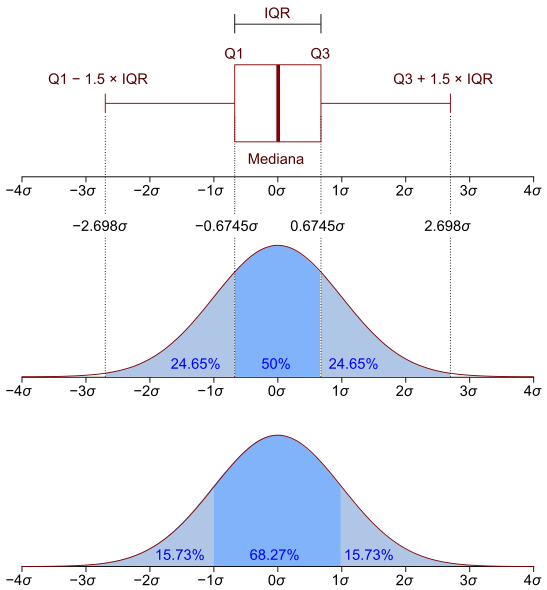
\includegraphics{img/da-data-cleaning/quantiles.png}

Джерело: https://en.wikipedia.org/wiki/Interquartile\_range

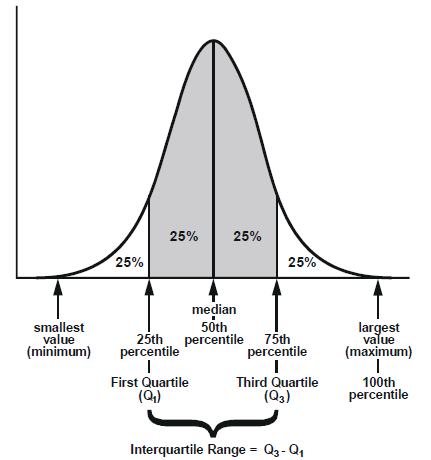
\includegraphics{img/da-data-cleaning/quantiles2.png}

Джерело:
https://makemeanalyst.com/explore-your-data-range-interquartile-range-and-box-plot/

Визначивши викиди у даних з ними можна здійснити кілька операцій:

\begin{enumerate}
\def\labelenumi{\arabic{enumi}.}
\tightlist
\item
  Заміна на деякі значення (impute)
\item
  Заміна на границі квантилей
\end{enumerate}

\begin{Shaded}
\begin{Highlighting}[]
\NormalTok{lower\_bound }\OtherTok{\textless{}{-}} \FunctionTok{quantile}\NormalTok{(river\_data}\SpecialCharTok{$}\NormalTok{nitrate, }\FloatTok{0.025}\NormalTok{)}
\NormalTok{lower\_bound}

\NormalTok{upper\_bound }\OtherTok{\textless{}{-}} \FunctionTok{quantile}\NormalTok{(river\_data}\SpecialCharTok{$}\NormalTok{nitrate, }\FloatTok{0.975}\NormalTok{)}
\NormalTok{upper\_bound}
\end{Highlighting}
\end{Shaded}

\textbf{2.5\%:} 0.75475

\textbf{97.5\%:} 1.4095

\begin{Shaded}
\begin{Highlighting}[]
\NormalTok{outlier\_index }\OtherTok{\textless{}{-}} \FunctionTok{which}\NormalTok{(river\_data}\SpecialCharTok{$}\NormalTok{nitrate }\SpecialCharTok{\textless{}}\NormalTok{ lower\_bound }\SpecialCharTok{|}\NormalTok{ river\_data}\SpecialCharTok{$}\NormalTok{nitrate }\SpecialCharTok{\textgreater{}}\NormalTok{ upper\_bound)}
\NormalTok{outlier\_index}
\end{Highlighting}
\end{Shaded}

\begin{enumerate}
\def\labelenumi{\arabic{enumi}.}
\tightlist
\item
  1
\item
  6
\item
  36
\item
  53
\item
  104
\item
  119
\item
  121
\item
  156
\item
  159
\item
  167
\item
  199
\item
  200
\item
  269
\item
  270
\item
  281
\item
  282
\end{enumerate}

\begin{Shaded}
\begin{Highlighting}[]
\NormalTok{river\_data[outlier\_index, ]}
\end{Highlighting}
\end{Shaded}

A data.frame: 16 × 3

\begin{longtable}[]{@{}
  >{\raggedright\arraybackslash}p{(\columnwidth - 6\tabcolsep) * \real{0.2500}}
  >{\raggedright\arraybackslash}p{(\columnwidth - 6\tabcolsep) * \real{0.2500}}
  >{\raggedright\arraybackslash}p{(\columnwidth - 6\tabcolsep) * \real{0.2500}}
  >{\raggedright\arraybackslash}p{(\columnwidth - 6\tabcolsep) * \real{0.2500}}@{}}
\toprule\noalign{}
\begin{minipage}[b]{\linewidth}\raggedright
\end{minipage} & \begin{minipage}[b]{\linewidth}\raggedright
index \textless int\textgreater{}
\end{minipage} & \begin{minipage}[b]{\linewidth}\raggedright
nitrate \textless dbl\textgreater{}
\end{minipage} & \begin{minipage}[b]{\linewidth}\raggedright
months \textless fct\textgreater{}
\end{minipage} \\
\midrule\noalign{}
\endhead
\bottomrule\noalign{}
\endlastfoot
1 & 1 & 1.581 & January \\
6 & 6 & 1.483 & June \\
36 & 36 & 1.643 & December \\
53 & 53 & 1.533 & May \\
104 & 104 & 0.671 & August \\
119 & 119 & 1.517 & November \\
121 & 121 & 1.414 & January \\
156 & 156 & 1.897 & December \\
159 & 159 & 1.414 & March \\
167 & 167 & 0.671 & November \\
199 & 199 & 0.748 & July \\
200 & 200 & 0.592 & August \\
269 & 269 & 0.700 & May \\
270 & 270 & 0.673 & June \\
281 & 281 & 0.730 & May \\
282 & 282 & 0.693 & June \\
\end{longtable}

Таким чином, усі значення вище та нище деякого показника можемо замінити
на потрібні нам значення, наприклад, середні за поточний місяць.

Здійснимо заміну значень у наборі даних на основі квантилей:

\begin{Shaded}
\begin{Highlighting}[]
\NormalTok{river\_data}\SpecialCharTok{$}\NormalTok{nitrate\_upd }\OtherTok{\textless{}{-}}\NormalTok{ river\_data}\SpecialCharTok{$}\NormalTok{nitrate}
\NormalTok{qnt }\OtherTok{\textless{}{-}} \FunctionTok{quantile}\NormalTok{(river\_data}\SpecialCharTok{$}\NormalTok{nitrate\_upd, }\AttributeTok{probs=}\FunctionTok{c}\NormalTok{(.}\DecValTok{05}\NormalTok{, .}\DecValTok{95}\NormalTok{), }\AttributeTok{na.rm =}\NormalTok{ T)}
\NormalTok{H }\OtherTok{\textless{}{-}} \FloatTok{1.5} \SpecialCharTok{*} \FunctionTok{IQR}\NormalTok{(qnt[}\DecValTok{1}\NormalTok{], }\AttributeTok{na.rm =}\NormalTok{ T)}
\NormalTok{river\_data}\SpecialCharTok{$}\NormalTok{nitrate\_upd[river\_data}\SpecialCharTok{$}\NormalTok{nitrate\_upd }\SpecialCharTok{\textless{}}\NormalTok{ (qnt[}\DecValTok{1}\NormalTok{] }\SpecialCharTok{{-}}\NormalTok{ H)] }\OtherTok{\textless{}{-}}\NormalTok{ qnt[}\DecValTok{1}\NormalTok{]}
\NormalTok{river\_data}\SpecialCharTok{$}\NormalTok{nitrate\_upd[river\_data}\SpecialCharTok{$}\NormalTok{nitrate\_upd }\SpecialCharTok{\textgreater{}}\NormalTok{ (qnt[}\DecValTok{2}\NormalTok{] }\SpecialCharTok{+}\NormalTok{ H)] }\OtherTok{\textless{}{-}}\NormalTok{ qnt[}\DecValTok{2}\NormalTok{]}

\NormalTok{qnt}
\end{Highlighting}
\end{Shaded}

\begin{description}
\tightlist
\item[5\%]
0.80595\%

1.3325
\end{description}

\begin{Shaded}
\begin{Highlighting}[]
\FunctionTok{boxplot}\NormalTok{(river\_data}\SpecialCharTok{$}\NormalTok{nitrate\_upd)}
\end{Highlighting}
\end{Shaded}

\includegraphics[width=4.375in,height=4.375in]{44-r-outliers_files/figure-pdf/cell-17-output-1.png}

\begin{Shaded}
\begin{Highlighting}[]
\FunctionTok{boxplot}\NormalTok{(nitrate\_upd }\SpecialCharTok{\textasciitilde{}}\NormalTok{ months, }\AttributeTok{data =}\NormalTok{ river\_data)}
\end{Highlighting}
\end{Shaded}

\includegraphics[width=4.375in,height=4.375in]{44-r-outliers_files/figure-pdf/cell-18-output-1.png}

\begin{Shaded}
\begin{Highlighting}[]
\FunctionTok{plot}\NormalTok{(nitrate\_upd }\SpecialCharTok{\textasciitilde{}}\NormalTok{ index, }\AttributeTok{data =}\NormalTok{ river\_data, }\AttributeTok{type =} \StringTok{"o"}\NormalTok{)}
\end{Highlighting}
\end{Shaded}

\includegraphics[width=4.375in,height=4.375in]{44-r-outliers_files/figure-pdf/cell-19-output-1.png}

\begin{center}\rule{0.5\linewidth}{0.5pt}\end{center}

\section{\texorpdfstring{Додаткові прийоми очистки даних
}{Додаткові прийоми очистки даних }}\label{ux434ux43eux434ux430ux442ux43aux43eux432ux456-ux43fux440ux438ux439ux43eux43cux438-ux43eux447ux438ux441ux442ux43aux438-ux434ux430ux43dux438ux445}

\subsection{Видалення
дублікатів}\label{ux432ux438ux434ux430ux43bux435ux43dux43dux44f-ux434ux443ux431ux43bux456ux43aux430ux442ux456ux432}

\begin{Shaded}
\begin{Highlighting}[]
\NormalTok{df }\OtherTok{\textless{}{-}} \FunctionTok{data.frame}\NormalTok{(}\AttributeTok{X =} \FunctionTok{c}\NormalTok{(}\DecValTok{1}\NormalTok{,}\DecValTok{1}\NormalTok{,}\DecValTok{2}\NormalTok{,}\DecValTok{1}\NormalTok{,}\DecValTok{3}\NormalTok{,}\DecValTok{2}\NormalTok{,}\DecValTok{1}\NormalTok{), }\AttributeTok{Y =} \FunctionTok{c}\NormalTok{(}\StringTok{"A"}\NormalTok{, }\StringTok{"B"}\NormalTok{, }\StringTok{"C"}\NormalTok{, }\StringTok{"A"}\NormalTok{, }\StringTok{"B"}\NormalTok{, }\StringTok{"C"}\NormalTok{, }\StringTok{"A"}\NormalTok{))}
\NormalTok{df}
\end{Highlighting}
\end{Shaded}

A data.frame: 7 × 2

\begin{longtable}[]{@{}ll@{}}
\toprule\noalign{}
X \textless dbl\textgreater{} & Y \textless chr\textgreater{} \\
\midrule\noalign{}
\endhead
\bottomrule\noalign{}
\endlastfoot
1 & A \\
1 & B \\
2 & C \\
1 & A \\
3 & B \\
2 & C \\
1 & A \\
\end{longtable}

\begin{Shaded}
\begin{Highlighting}[]
\NormalTok{df }\SpecialCharTok{|\textgreater{}} \FunctionTok{distinct}\NormalTok{()}
\end{Highlighting}
\end{Shaded}

A data.frame: 4 × 2

\begin{longtable}[]{@{}ll@{}}
\toprule\noalign{}
X \textless dbl\textgreater{} & Y \textless chr\textgreater{} \\
\midrule\noalign{}
\endhead
\bottomrule\noalign{}
\endlastfoot
1 & A \\
1 & B \\
2 & C \\
3 & B \\
\end{longtable}

\begin{center}\rule{0.5\linewidth}{0.5pt}\end{center}

\section{Набори
даних}\label{ux43dux430ux431ux43eux440ux438-ux434ux430ux43dux438ux445-11}

\begin{enumerate}
\def\labelenumi{\arabic{enumi}.}
\tightlist
\item
  https://github.com/kleban/r-book-published/tree/main/datasets/untitled.csv
\item
  https://github.com/kleban/r-book-published/tree/main/datasets/badtitled.csv
\item
  https://github.com/kleban/r-book-published/tree/main/datasets/cleaned\_titled.csv
\item
  https://github.com/kleban/r-book-published/tree/main/datasets/cleaned\_titled2.csv
\item
  https://github.com/kleban/r-book-published/tree/main/datasets/river\_eco.csv
\end{enumerate}

\begin{center}\rule{0.5\linewidth}{0.5pt}\end{center}

\section{Використані та додаткові
джерела}\label{ux432ux438ux43aux43eux440ux438ux441ux442ux430ux43dux456-ux442ux430-ux434ux43eux434ux430ux442ux43aux43eux432ux456-ux434ux436ux435ux440ux435ux43bux430-4}

\begin{enumerate}
\def\labelenumi{\arabic{enumi}.}
\tightlist
\item
  \href{https://www.insidesherpa.com/virtual-internships/m7W4GMqeT3bh9Nb2c}{KPMG
  Virtual Internship}
\item
  \href{https://cran.r-project.org/doc/contrib/de_Jonge+van_der_Loo-Introduction_to_data_cleaning_with_R.pdf}{An
  introduction to data cleaning with R / Edwin de Jonge, Mark van der
  Loo, 2013}
\item
  \href{datacamp.com/courses/anomaly-detection-in-r}{Anomaly Detection
  in R}
\item
  \href{https://medium.com/analytics-vidhya/k-nearest-neighbor-the-maths-behind-it-how-it-works-and-an-example-f1de1208546c}{K-nearest
  Neighbor: The maths behind it, how it works and an example}
\item
  \href{https://en.wikipedia.org/wiki/Quantile}{Quantile. Wikipedia}
\end{enumerate}

\part{ТЕМА 5. КОНСТРУЮВАННЯ ОЗНАК}

\chapter{Feature engineering in R}\label{feature-engineering-in-r}

\begin{center}\rule{0.5\linewidth}{0.5pt}\end{center}

You need this packages for code execution:

\begin{Shaded}
\begin{Highlighting}[]
\CommentTok{\# install.packages("ggplot2")}
\FunctionTok{install.packages}\NormalTok{(}\StringTok{"gridExtra"}\NormalTok{)}
\CommentTok{\# install.packages("scorecard")}
\CommentTok{\# install.packages("caret")}
\CommentTok{\# install.packages("gmodels")}
\CommentTok{\# install.packages("superml") \#you olso need R6 package}
\end{Highlighting}
\end{Shaded}

\begin{verbatim}
package 'gridExtra' successfully unpacked and MD5 sums checked

The downloaded binary packages are in
    D:\Temp\Rtmpum9OKD\downloaded_packages
\end{verbatim}

\begin{Shaded}
\begin{Highlighting}[]
\FunctionTok{invisible}\NormalTok{(}\FunctionTok{Sys.setlocale}\NormalTok{(}\StringTok{"LC\_ALL"}\NormalTok{, }\StringTok{"Ukrainian"}\NormalTok{))}
\FunctionTok{invisible}\NormalTok{(}\FunctionTok{options}\NormalTok{(}\AttributeTok{warn=}\SpecialCharTok{{-}}\DecValTok{1}\NormalTok{))}
\end{Highlighting}
\end{Shaded}

\begin{center}\rule{0.5\linewidth}{0.5pt}\end{center}

\section{What's Feature Engineering?}\label{whats-feature-engineering}

\texttt{Feature\ engineering} is the most important technique used in
creating machine learning models.

Feature Engineering is a basic term used to cover many operations that
are performed on the variables(features) to fit them into the algorithm.
\textbf{It helps in increasing the accuracy} of the model thereby
enhances the results of the predictions. Feature Engineered machine
learning models perform better on data than basic machine learning
models. The following aspects of feature engineering are as follows
{[}1{]}:

\begin{enumerate}
\def\labelenumi{\arabic{enumi}.}
\tightlist
\item
  \texttt{Feature\ Scaling}: It is done to get the features on the same
  scale( for eg. Euclidean distance).
\item
  \texttt{Feature\ Transformation}: It is done to normalize the
  data(feature) by a function.
\item
  \texttt{Feature\ Construction}: It is done to create new features
  based on original descriptors to improve the accuracy of the
  predictive model.
\end{enumerate}

A \texttt{"feature"} in the context of predictive modeling is just
another name for a \texttt{predictor\ variable}. Feature engineering is
the general term for creating and manipulating predictors so that a good
predictive model can be created.

\begin{center}\rule{0.5\linewidth}{0.5pt}\end{center}

\section{Feature Scaling}\label{feature-scaling}

\texttt{Feature\ Scaling} refers to putting the values in the same range
or same scale so that no variable is dominated by the other.

Most of the times, your dataset will contain features highly varying in
magnitudes, units and range. But since, most of the machine learning
algorithms use Euclidean distance between two data points in their
computations, this is a problem.

If left alone, these algorithms only take in the magnitude of features
neglecting the units. The results would vary greatly between different
units, 5kg and 5000gms. The features with high magnitudes will weigh in
a lot more in the distance calculations than features with low
magnitudes. To suppress this effect, we need to bring all features to
the same level of magnitudes. This can be achieved by scaling.

Here's the curious thing about feature scaling -- it improves
(significantly) the performance of some machine learning algorithms and
does not work at all for others.

Also, what's the difference between normalization and standardization?
These are two of the most commonly used feature scaling techniques in
machine learning but a level of ambiguity exists in their understanding.

\begin{center}\rule{0.5\linewidth}{0.5pt}\end{center}

\subsection{Normalization}\label{normalization}

\subsubsection{Theory}\label{theory}

\textbf{Normalization} is a scaling technique in which values are
shifted and rescaled so that they end up ranging between 0 and 1. It is
also known as \textbf{\texttt{Min-Max\ scaling}}.

Here's the formula for normalization:

\(X' = \frac{X-X_{min}}{X_{max} - X_{min}}\)

Here, \(X_{max}\) and \(X_{min}\) are the maximum and the minimum values
of the feature respectively.

When the value of \(X\) is the minimum value in the column, the
numerator will be \(0\), and hence \(X'\) is \(0\).

On the other hand, when the value of \(X\) is the maximum value in the
column, the numerator is equal to the denominator and thus the value of
\(X'\) is \(1\).

If the value of \(X\) is between the minimum and the maximum value, then
the value of \(X'\) is between \(0\) and \(1\).

\begin{center}\rule{0.5\linewidth}{0.5pt}\end{center}

\subsubsection{Practice}\label{practice}

So, let's implement own normalization function.

\begin{Shaded}
\begin{Highlighting}[]
\CommentTok{\# Lets use client churn dataset from telco: https://www.kaggle.com/blastchar/telco{-}customer{-}churn}
\NormalTok{churn\_data }\OtherTok{\textless{}{-}} \FunctionTok{read.csv}\NormalTok{(}\StringTok{"data/telecom\_users.csv"}\NormalTok{)}
\FunctionTok{head}\NormalTok{(churn\_data)}
\end{Highlighting}
\end{Shaded}

A data.frame: 6 × 22

\begin{longtable}[]{@{}
  >{\raggedright\arraybackslash}p{(\columnwidth - 42\tabcolsep) * \real{0.0455}}
  >{\raggedright\arraybackslash}p{(\columnwidth - 42\tabcolsep) * \real{0.0455}}
  >{\raggedright\arraybackslash}p{(\columnwidth - 42\tabcolsep) * \real{0.0455}}
  >{\raggedright\arraybackslash}p{(\columnwidth - 42\tabcolsep) * \real{0.0455}}
  >{\raggedright\arraybackslash}p{(\columnwidth - 42\tabcolsep) * \real{0.0455}}
  >{\raggedright\arraybackslash}p{(\columnwidth - 42\tabcolsep) * \real{0.0455}}
  >{\raggedright\arraybackslash}p{(\columnwidth - 42\tabcolsep) * \real{0.0455}}
  >{\raggedright\arraybackslash}p{(\columnwidth - 42\tabcolsep) * \real{0.0455}}
  >{\raggedright\arraybackslash}p{(\columnwidth - 42\tabcolsep) * \real{0.0455}}
  >{\raggedright\arraybackslash}p{(\columnwidth - 42\tabcolsep) * \real{0.0455}}
  >{\raggedright\arraybackslash}p{(\columnwidth - 42\tabcolsep) * \real{0.0455}}
  >{\raggedright\arraybackslash}p{(\columnwidth - 42\tabcolsep) * \real{0.0455}}
  >{\raggedright\arraybackslash}p{(\columnwidth - 42\tabcolsep) * \real{0.0455}}
  >{\raggedright\arraybackslash}p{(\columnwidth - 42\tabcolsep) * \real{0.0455}}
  >{\raggedright\arraybackslash}p{(\columnwidth - 42\tabcolsep) * \real{0.0455}}
  >{\raggedright\arraybackslash}p{(\columnwidth - 42\tabcolsep) * \real{0.0455}}
  >{\raggedright\arraybackslash}p{(\columnwidth - 42\tabcolsep) * \real{0.0455}}
  >{\raggedright\arraybackslash}p{(\columnwidth - 42\tabcolsep) * \real{0.0455}}
  >{\raggedright\arraybackslash}p{(\columnwidth - 42\tabcolsep) * \real{0.0455}}
  >{\raggedright\arraybackslash}p{(\columnwidth - 42\tabcolsep) * \real{0.0455}}
  >{\raggedright\arraybackslash}p{(\columnwidth - 42\tabcolsep) * \real{0.0455}}
  >{\raggedright\arraybackslash}p{(\columnwidth - 42\tabcolsep) * \real{0.0455}}@{}}
\toprule\noalign{}
\begin{minipage}[b]{\linewidth}\raggedright
\end{minipage} & \begin{minipage}[b]{\linewidth}\raggedright
X \textless int\textgreater{}
\end{minipage} & \begin{minipage}[b]{\linewidth}\raggedright
customerID \textless chr\textgreater{}
\end{minipage} & \begin{minipage}[b]{\linewidth}\raggedright
gender \textless chr\textgreater{}
\end{minipage} & \begin{minipage}[b]{\linewidth}\raggedright
SeniorCitizen \textless int\textgreater{}
\end{minipage} & \begin{minipage}[b]{\linewidth}\raggedright
Partner \textless chr\textgreater{}
\end{minipage} & \begin{minipage}[b]{\linewidth}\raggedright
Dependents \textless chr\textgreater{}
\end{minipage} & \begin{minipage}[b]{\linewidth}\raggedright
tenure \textless int\textgreater{}
\end{minipage} & \begin{minipage}[b]{\linewidth}\raggedright
PhoneService \textless chr\textgreater{}
\end{minipage} & \begin{minipage}[b]{\linewidth}\raggedright
MultipleLines \textless chr\textgreater{}
\end{minipage} & \begin{minipage}[b]{\linewidth}\raggedright
InternetService \textless chr\textgreater{}
\end{minipage} & \begin{minipage}[b]{\linewidth}\raggedright
⋯ ⋯
\end{minipage} & \begin{minipage}[b]{\linewidth}\raggedright
DeviceProtection \textless chr\textgreater{}
\end{minipage} & \begin{minipage}[b]{\linewidth}\raggedright
TechSupport \textless chr\textgreater{}
\end{minipage} & \begin{minipage}[b]{\linewidth}\raggedright
StreamingTV \textless chr\textgreater{}
\end{minipage} & \begin{minipage}[b]{\linewidth}\raggedright
StreamingMovies \textless chr\textgreater{}
\end{minipage} & \begin{minipage}[b]{\linewidth}\raggedright
Contract \textless chr\textgreater{}
\end{minipage} & \begin{minipage}[b]{\linewidth}\raggedright
PaperlessBilling \textless chr\textgreater{}
\end{minipage} & \begin{minipage}[b]{\linewidth}\raggedright
PaymentMethod \textless chr\textgreater{}
\end{minipage} & \begin{minipage}[b]{\linewidth}\raggedright
MonthlyCharges \textless chr\textgreater{}
\end{minipage} & \begin{minipage}[b]{\linewidth}\raggedright
TotalCharges \textless dbl\textgreater{}
\end{minipage} & \begin{minipage}[b]{\linewidth}\raggedright
Churn \textless chr\textgreater{}
\end{minipage} \\
\midrule\noalign{}
\endhead
\bottomrule\noalign{}
\endlastfoot
1 & 1869 & 7010-BRBUU & Male & 0 & Yes & Yes & 72 & Yes & Yes & No & ⋯ &
No internet service & No internet service & No internet service & No
internet service & Two year & No & Credit card (automatic) & 24.1 &
1734.65 & No \\
2 & 4528 & 9688-YGXVR & Female & 0 & No & No & 44 & Yes & No & Fiber
optic & ⋯ & Yes & No & Yes & No & Month-to-month & Yes & Credit card
(automatic) & 88.15 & 3973.20 & No \\
3 & 6344 & 9286-DOJGF & Female & 1 & Yes & No & 38 & Yes & Yes & Fiber
optic & ⋯ & No & No & No & No & Month-to-month & Yes & Bank transfer
(automatic) & 74.95 & 2869.85 & Yes \\
4 & 6739 & 6994-KERXL & Male & 0 & No & No & 4 & Yes & No & DSL & ⋯ & No
& No & No & Yes & Month-to-month & Yes & Electronic check & 55.9 &
238.50 & No \\
5 & 432 & 2181-UAESM & Male & 0 & No & No & 2 & Yes & No & DSL & ⋯ & Yes
& No & No & No & Month-to-month & No & Electronic check & 53.45 & 119.50
& No \\
6 & 2215 & 4312-GVYNH & Female & 0 & Yes & No & 70 & No & No phone
service & DSL & ⋯ & Yes & Yes & No & Yes & Two year & Yes & Bank
transfer (automatic) & 49.85 & 3370.20 & No \\
\end{longtable}

\begin{Shaded}
\begin{Highlighting}[]
\FunctionTok{str}\NormalTok{(churn\_data)}
\end{Highlighting}
\end{Shaded}

\begin{verbatim}
'data.frame':   5986 obs. of  22 variables:
 $ X               : int  1869 4528 6344 6739 432 2215 5260 6001 1480 5137 ...
 $ customerID      : chr  "7010-BRBUU" "9688-YGXVR" "9286-DOJGF" "6994-KERXL" ...
 $ gender          : chr  "Male" "Female" "Female" "Male" ...
 $ SeniorCitizen   : int  0 0 1 0 0 0 0 0 0 1 ...
 $ Partner         : chr  "Yes" "No" "Yes" "No" ...
 $ Dependents      : chr  "Yes" "No" "No" "No" ...
 $ tenure          : int  72 44 38 4 2 70 33 1 39 55 ...
 $ PhoneService    : chr  "Yes" "Yes" "Yes" "Yes" ...
 $ MultipleLines   : chr  "Yes" "No" "Yes" "No" ...
 $ InternetService : chr  "No" "Fiber optic" "Fiber optic" "DSL" ...
 $ OnlineSecurity  : chr  "No internet service" "No" "No" "No" ...
 $ OnlineBackup    : chr  "No internet service" "Yes" "No" "No" ...
 $ DeviceProtection: chr  "No internet service" "Yes" "No" "No" ...
 $ TechSupport     : chr  "No internet service" "No" "No" "No" ...
 $ StreamingTV     : chr  "No internet service" "Yes" "No" "No" ...
 $ StreamingMovies : chr  "No internet service" "No" "No" "Yes" ...
 $ Contract        : chr  "Two year" "Month-to-month" "Month-to-month" "Month-to-month" ...
 $ PaperlessBilling: chr  "No" "Yes" "Yes" "Yes" ...
 $ PaymentMethod   : chr  "Credit card (automatic)" "Credit card (automatic)" "Bank transfer (automatic)" "Electronic check" ...
 $ MonthlyCharges  : chr  "24.1" "88.15" "74.95" "55.9" ...
 $ TotalCharges    : num  1735 3973 2870 238 120 ...
 $ Churn           : chr  "No" "No" "Yes" "No" ...
\end{verbatim}

\begin{Shaded}
\begin{Highlighting}[]
\CommentTok{\# next check summary of values}
\FunctionTok{summary}\NormalTok{(churn\_data)}

\CommentTok{\# check TotalCharges field}
\end{Highlighting}
\end{Shaded}

\begin{verbatim}
       X         customerID           gender          SeniorCitizen   
 Min.   :   0   Length:5986        Length:5986        Min.   :0.0000  
 1st Qu.:1777   Class :character   Class :character   1st Qu.:0.0000  
 Median :3546   Mode  :character   Mode  :character   Median :0.0000  
 Mean   :3534                                         Mean   :0.1614  
 3rd Qu.:5292                                         3rd Qu.:0.0000  
 Max.   :7042                                         Max.   :1.0000  
                                                                      
   Partner           Dependents            tenure      PhoneService      
 Length:5986        Length:5986        Min.   : 0.00   Length:5986       
 Class :character   Class :character   1st Qu.: 9.00   Class :character  
 Mode  :character   Mode  :character   Median :29.00   Mode  :character  
                                       Mean   :32.47                     
                                       3rd Qu.:56.00                     
                                       Max.   :72.00                     
                                                                         
 MultipleLines      InternetService    OnlineSecurity     OnlineBackup      
 Length:5986        Length:5986        Length:5986        Length:5986       
 Class :character   Class :character   Class :character   Class :character  
 Mode  :character   Mode  :character   Mode  :character   Mode  :character  
                                                                            
                                                                            
                                                                            
                                                                            
 DeviceProtection   TechSupport        StreamingTV        StreamingMovies   
 Length:5986        Length:5986        Length:5986        Length:5986       
 Class :character   Class :character   Class :character   Class :character  
 Mode  :character   Mode  :character   Mode  :character   Mode  :character  
                                                                            
                                                                            
                                                                            
                                                                            
   Contract         PaperlessBilling   PaymentMethod      MonthlyCharges    
 Length:5986        Length:5986        Length:5986        Length:5986       
 Class :character   Class :character   Class :character   Class :character  
 Mode  :character   Mode  :character   Mode  :character   Mode  :character  
                                                                            
                                                                            
                                                                            
                                                                            
  TotalCharges       Churn          
 Min.   :  18.8   Length:5986       
 1st Qu.: 404.3   Class :character  
 Median :1412.2   Mode  :character  
 Mean   :2298.1                     
 3rd Qu.:3847.0                     
 Max.   :8684.8                     
 NA's   :10                         
\end{verbatim}

Next, lets build histogram of \texttt{Income} and check how it splited
with \texttt{ggplot2}:

\begin{Shaded}
\begin{Highlighting}[]
\CommentTok{\#install.packages("ggplot2")}
\FunctionTok{library}\NormalTok{(ggplot2)}
\end{Highlighting}
\end{Shaded}

\texttt{ggplot()} - function for building charts

\texttt{data} - first parameter - dataset

\texttt{aes()} - authetics - visualition axis / Construct aesthetic
mappings

\texttt{geom\_CHART\_TYPE()} - set the chart type

\texttt{geom\_histogram()} - Histograms and frequency polygons

//\texttt{theme\_set()} - theme configutation

\begin{Shaded}
\begin{Highlighting}[]
\FunctionTok{library}\NormalTok{(ggplot2)}
\FunctionTok{ggplot}\NormalTok{(}\AttributeTok{data =}\NormalTok{ churn\_data, }\FunctionTok{aes}\NormalTok{(}\AttributeTok{x=}\NormalTok{TotalCharges)) }\SpecialCharTok{+} \FunctionTok{geom\_histogram}\NormalTok{(}\AttributeTok{bins =} \DecValTok{15}\NormalTok{)}

\CommentTok{\# try theme}
\end{Highlighting}
\end{Shaded}

\begin{verbatim}
Warning message:
"Removed 10 rows containing non-finite values (stat_bin)."
\end{verbatim}

\includegraphics[width=4.375in,height=4.375in]{etl-feature-engineering_files/figure-pdf/cell-8-output-2.png}

\begin{Shaded}
\begin{Highlighting}[]
\CommentTok{\# Lets replace missing with 0 zero for TotalCharges }
\FunctionTok{library}\NormalTok{(magrittr) }\CommentTok{\# if pipe not loaded}
\FunctionTok{library}\NormalTok{(dplyr) }\CommentTok{\# for mutate function}
\NormalTok{churn\_data }\OtherTok{\textless{}{-}}\NormalTok{ churn\_data }\SpecialCharTok{\%\textgreater{}\%}
            \FunctionTok{mutate}\NormalTok{(}\AttributeTok{TotalCharges =} \FunctionTok{ifelse}\NormalTok{(}\FunctionTok{is.na}\NormalTok{(TotalCharges), }\DecValTok{0}\NormalTok{ , TotalCharges))}

\FunctionTok{ggplot}\NormalTok{(churn\_data, }\FunctionTok{aes}\NormalTok{(}\AttributeTok{x=}\NormalTok{TotalCharges)) }\SpecialCharTok{+} \FunctionTok{geom\_histogram}\NormalTok{(}\AttributeTok{bins =} \DecValTok{15}\NormalTok{)}
\end{Highlighting}
\end{Shaded}

\begin{verbatim}

Attaching package: 'dplyr'


The following objects are masked from 'package:stats':

    filter, lag


The following objects are masked from 'package:base':

    intersect, setdiff, setequal, union

\end{verbatim}

\includegraphics[width=4.375in,height=4.375in]{etl-feature-engineering_files/figure-pdf/cell-9-output-2.png}

\begin{Shaded}
\begin{Highlighting}[]
\CommentTok{\# Lets implement own normalization function by fomula explained earlie}
\NormalTok{normalizeData }\OtherTok{\textless{}{-}} \ControlFlowTok{function}\NormalTok{(x) \{}
    \FunctionTok{return}\NormalTok{ ((x }\SpecialCharTok{{-}} \FunctionTok{min}\NormalTok{(x)) }\SpecialCharTok{/}\NormalTok{ (}\FunctionTok{max}\NormalTok{(x) }\SpecialCharTok{{-}} \FunctionTok{min}\NormalTok{(x)))}
\NormalTok{\}}
\end{Highlighting}
\end{Shaded}

\begin{Shaded}
\begin{Highlighting}[]
\FunctionTok{library}\NormalTok{(dplyr)}
\CommentTok{\# Normalize TotalCharges}
\NormalTok{churn\_data }\OtherTok{\textless{}{-}}\NormalTok{ churn\_data }\SpecialCharTok{|\textgreater{}}
    \FunctionTok{filter}\NormalTok{(}\SpecialCharTok{!}\FunctionTok{is.na}\NormalTok{(TotalCharges)) }\SpecialCharTok{|\textgreater{}}
    \FunctionTok{mutate}\NormalTok{(}\AttributeTok{TotalChargesNorm =} \FunctionTok{normalizeData}\NormalTok{(TotalCharges))}

\NormalTok{churn\_data }\SpecialCharTok{\%\textgreater{}\%} \FunctionTok{head}\NormalTok{() }\CommentTok{\# check the last columns}
\end{Highlighting}
\end{Shaded}

A data.frame: 6 × 23

\begin{longtable}[]{@{}
  >{\raggedright\arraybackslash}p{(\columnwidth - 42\tabcolsep) * \real{0.0455}}
  >{\raggedright\arraybackslash}p{(\columnwidth - 42\tabcolsep) * \real{0.0455}}
  >{\raggedright\arraybackslash}p{(\columnwidth - 42\tabcolsep) * \real{0.0455}}
  >{\raggedright\arraybackslash}p{(\columnwidth - 42\tabcolsep) * \real{0.0455}}
  >{\raggedright\arraybackslash}p{(\columnwidth - 42\tabcolsep) * \real{0.0455}}
  >{\raggedright\arraybackslash}p{(\columnwidth - 42\tabcolsep) * \real{0.0455}}
  >{\raggedright\arraybackslash}p{(\columnwidth - 42\tabcolsep) * \real{0.0455}}
  >{\raggedright\arraybackslash}p{(\columnwidth - 42\tabcolsep) * \real{0.0455}}
  >{\raggedright\arraybackslash}p{(\columnwidth - 42\tabcolsep) * \real{0.0455}}
  >{\raggedright\arraybackslash}p{(\columnwidth - 42\tabcolsep) * \real{0.0455}}
  >{\raggedright\arraybackslash}p{(\columnwidth - 42\tabcolsep) * \real{0.0455}}
  >{\raggedright\arraybackslash}p{(\columnwidth - 42\tabcolsep) * \real{0.0455}}
  >{\raggedright\arraybackslash}p{(\columnwidth - 42\tabcolsep) * \real{0.0455}}
  >{\raggedright\arraybackslash}p{(\columnwidth - 42\tabcolsep) * \real{0.0455}}
  >{\raggedright\arraybackslash}p{(\columnwidth - 42\tabcolsep) * \real{0.0455}}
  >{\raggedright\arraybackslash}p{(\columnwidth - 42\tabcolsep) * \real{0.0455}}
  >{\raggedright\arraybackslash}p{(\columnwidth - 42\tabcolsep) * \real{0.0455}}
  >{\raggedright\arraybackslash}p{(\columnwidth - 42\tabcolsep) * \real{0.0455}}
  >{\raggedright\arraybackslash}p{(\columnwidth - 42\tabcolsep) * \real{0.0455}}
  >{\raggedright\arraybackslash}p{(\columnwidth - 42\tabcolsep) * \real{0.0455}}
  >{\raggedright\arraybackslash}p{(\columnwidth - 42\tabcolsep) * \real{0.0455}}
  >{\raggedright\arraybackslash}p{(\columnwidth - 42\tabcolsep) * \real{0.0455}}@{}}
\toprule\noalign{}
\begin{minipage}[b]{\linewidth}\raggedright
\end{minipage} & \begin{minipage}[b]{\linewidth}\raggedright
X \textless int\textgreater{}
\end{minipage} & \begin{minipage}[b]{\linewidth}\raggedright
customerID \textless chr\textgreater{}
\end{minipage} & \begin{minipage}[b]{\linewidth}\raggedright
gender \textless chr\textgreater{}
\end{minipage} & \begin{minipage}[b]{\linewidth}\raggedright
SeniorCitizen \textless int\textgreater{}
\end{minipage} & \begin{minipage}[b]{\linewidth}\raggedright
Partner \textless chr\textgreater{}
\end{minipage} & \begin{minipage}[b]{\linewidth}\raggedright
Dependents \textless chr\textgreater{}
\end{minipage} & \begin{minipage}[b]{\linewidth}\raggedright
tenure \textless int\textgreater{}
\end{minipage} & \begin{minipage}[b]{\linewidth}\raggedright
PhoneService \textless chr\textgreater{}
\end{minipage} & \begin{minipage}[b]{\linewidth}\raggedright
MultipleLines \textless chr\textgreater{}
\end{minipage} & \begin{minipage}[b]{\linewidth}\raggedright
InternetService \textless chr\textgreater{}
\end{minipage} & \begin{minipage}[b]{\linewidth}\raggedright
⋯ ⋯
\end{minipage} & \begin{minipage}[b]{\linewidth}\raggedright
TechSupport \textless chr\textgreater{}
\end{minipage} & \begin{minipage}[b]{\linewidth}\raggedright
StreamingTV \textless chr\textgreater{}
\end{minipage} & \begin{minipage}[b]{\linewidth}\raggedright
StreamingMovies \textless chr\textgreater{}
\end{minipage} & \begin{minipage}[b]{\linewidth}\raggedright
Contract \textless chr\textgreater{}
\end{minipage} & \begin{minipage}[b]{\linewidth}\raggedright
PaperlessBilling \textless chr\textgreater{}
\end{minipage} & \begin{minipage}[b]{\linewidth}\raggedright
PaymentMethod \textless chr\textgreater{}
\end{minipage} & \begin{minipage}[b]{\linewidth}\raggedright
MonthlyCharges \textless chr\textgreater{}
\end{minipage} & \begin{minipage}[b]{\linewidth}\raggedright
TotalCharges \textless dbl\textgreater{}
\end{minipage} & \begin{minipage}[b]{\linewidth}\raggedright
Churn \textless chr\textgreater{}
\end{minipage} & \begin{minipage}[b]{\linewidth}\raggedright
TotalChargesNorm \textless dbl\textgreater{}
\end{minipage} \\
\midrule\noalign{}
\endhead
\bottomrule\noalign{}
\endlastfoot
1 & 1869 & 7010-BRBUU & Male & 0 & Yes & Yes & 72 & Yes & Yes & No & ⋯ &
No internet service & No internet service & No internet service & Two
year & No & Credit card (automatic) & 24.1 & 1734.65 & No &
0.19799792 \\
2 & 4528 & 9688-YGXVR & Female & 0 & No & No & 44 & Yes & No & Fiber
optic & ⋯ & No & Yes & No & Month-to-month & Yes & Credit card
(automatic) & 88.15 & 3973.20 & No & 0.45631202 \\
3 & 6344 & 9286-DOJGF & Female & 1 & Yes & No & 38 & Yes & Yes & Fiber
optic & ⋯ & No & No & No & Month-to-month & Yes & Bank transfer
(automatic) & 74.95 & 2869.85 & Yes & 0.32899261 \\
4 & 6739 & 6994-KERXL & Male & 0 & No & No & 4 & Yes & No & DSL & ⋯ & No
& No & Yes & Month-to-month & Yes & Electronic check & 55.9 & 238.50 &
No & 0.02535195 \\
5 & 432 & 2181-UAESM & Male & 0 & No & No & 2 & Yes & No & DSL & ⋯ & No
& No & No & Month-to-month & No & Electronic check & 53.45 & 119.50 & No
& 0.01162012 \\
6 & 2215 & 4312-GVYNH & Female & 0 & Yes & No & 70 & No & No phone
service & DSL & ⋯ & Yes & No & Yes & Two year & Yes & Bank transfer
(automatic) & 49.85 & 3370.20 & No & 0.38672975 \\
\end{longtable}

\begin{Shaded}
\begin{Highlighting}[]
\CommentTok{\#summary for the last field}
\FunctionTok{summary}\NormalTok{(churn\_data}\SpecialCharTok{$}\NormalTok{TotalChargesNorm)}

\CommentTok{\#its from 1 to zero}
\end{Highlighting}
\end{Shaded}

\begin{verbatim}
   Min. 1st Qu.  Median    Mean 3rd Qu.    Max. 
0.00000 0.04449 0.16078 0.26301 0.44174 1.00000 
\end{verbatim}

\begin{Shaded}
\begin{Highlighting}[]
\CommentTok{\# And lets make a histogram}
\FunctionTok{ggplot}\NormalTok{(churn\_data, }\FunctionTok{aes}\NormalTok{(}\AttributeTok{x=}\NormalTok{TotalChargesNorm)) }\SpecialCharTok{+} \FunctionTok{geom\_histogram}\NormalTok{(}\AttributeTok{bins =} \DecValTok{15}\NormalTok{)}
\end{Highlighting}
\end{Shaded}

\includegraphics[width=4.375in,height=4.375in]{etl-feature-engineering_files/figure-pdf/cell-14-output-1.png}

We observe identical histograms even though the
\texttt{TotalCharges\ /\ TotalChargesNorm} axis is rescaled.

Therefore we show that \textbf{normalization didn't affect the
distribution properties} of the rescaled data.

\begin{center}\rule{0.5\linewidth}{0.5pt}\end{center}

\subsection{Standardization}\label{standardization}

\subsubsection{Theory}\label{theory-1}

\texttt{Standardization} is another scaling technique where the values
are centered around the mean with a unit standard deviation. This means
that the mean of the attribute becomes zero and the resultant
distribution has a unit standard deviation.

Here's the formula for standardization:

\(X' = \frac{X-\mu}{\sigma}\)

Feature scaling: \(\mu\) is the mean of the feature values and Feature
scaling: \(\sigma\) is the standard deviation of the feature values.
Note that in this case, the values are not restricted to a particular
range.

Now, the big question in your mind must be when should we use
normalization and when should we use standardization?

Normalization vs.~standardization is an eternal question among machine
learning newcomers. Let me elaborate on the answer in this section.

Normalization is good to use when you know that the distribution of your
data does not follow a Gaussian distribution. This can be useful in
algorithms that do not assume any distribution of the data like
K-Nearest Neighbors and Neural Networks.

Standardization, on the other hand, can be helpful in cases where the
data follows a Gaussian distribution. However, this does not have to be
necessarily true. Also, unlike normalization, standardization does not
have a bounding range. So, even if you have outliers in your data, they
will not be affected by standardization. However, at the end of the day,
the choice of using normalization or standardization will depend on your
problem and the machine learning algorithm you are using. There is no
hard and fast rule to tell you when to normalize or standardize your
data. You can always start by fitting your model to raw, normalized and
standardized data and compare the performance for best results.

It is a good practice to fit the scaler on the training data and then
use it to transform the testing data. This would avoid any data leakage
during the model testing process. Also, the scaling of target values is
generally not required.

\begin{center}\rule{0.5\linewidth}{0.5pt}\end{center}

\subsubsection{Practice}\label{practice-1}

Lets write own function for standartization:

\begin{Shaded}
\begin{Highlighting}[]
\CommentTok{\# if sdev is NA {-} calculate start deviation from data}

\NormalTok{standartize }\OtherTok{\textless{}{-}} \ControlFlowTok{function}\NormalTok{(data) \{    }
\NormalTok{    sdev }\OtherTok{=} \FunctionTok{sd}\NormalTok{(data, }\AttributeTok{na.rm =} \ConstantTok{TRUE}\NormalTok{)  }
\NormalTok{    data }\OtherTok{\textless{}{-}}\NormalTok{ (data }\SpecialCharTok{{-}} \FunctionTok{mean}\NormalTok{(data, }\AttributeTok{na.rm =}\NormalTok{ T)) }\SpecialCharTok{/}\NormalTok{ sdev}
    \FunctionTok{return}\NormalTok{ (data)    }
\NormalTok{\}}
\end{Highlighting}
\end{Shaded}

\begin{Shaded}
\begin{Highlighting}[]
\CommentTok{\# Normalize TotalCharges}
\NormalTok{churn\_data }\OtherTok{\textless{}{-}}\NormalTok{ churn\_data }\SpecialCharTok{\%\textgreater{}\%}
    \FunctionTok{mutate}\NormalTok{(}\AttributeTok{TotalChargesStand =} \FunctionTok{standartize}\NormalTok{(TotalCharges))}

\NormalTok{churn\_data }\SpecialCharTok{\%\textgreater{}\%} \FunctionTok{head}\NormalTok{() }\CommentTok{\# check the last columns}
\end{Highlighting}
\end{Shaded}

A data.frame: 6 × 24

\begin{longtable}[]{@{}
  >{\raggedright\arraybackslash}p{(\columnwidth - 42\tabcolsep) * \real{0.0455}}
  >{\raggedright\arraybackslash}p{(\columnwidth - 42\tabcolsep) * \real{0.0455}}
  >{\raggedright\arraybackslash}p{(\columnwidth - 42\tabcolsep) * \real{0.0455}}
  >{\raggedright\arraybackslash}p{(\columnwidth - 42\tabcolsep) * \real{0.0455}}
  >{\raggedright\arraybackslash}p{(\columnwidth - 42\tabcolsep) * \real{0.0455}}
  >{\raggedright\arraybackslash}p{(\columnwidth - 42\tabcolsep) * \real{0.0455}}
  >{\raggedright\arraybackslash}p{(\columnwidth - 42\tabcolsep) * \real{0.0455}}
  >{\raggedright\arraybackslash}p{(\columnwidth - 42\tabcolsep) * \real{0.0455}}
  >{\raggedright\arraybackslash}p{(\columnwidth - 42\tabcolsep) * \real{0.0455}}
  >{\raggedright\arraybackslash}p{(\columnwidth - 42\tabcolsep) * \real{0.0455}}
  >{\raggedright\arraybackslash}p{(\columnwidth - 42\tabcolsep) * \real{0.0455}}
  >{\raggedright\arraybackslash}p{(\columnwidth - 42\tabcolsep) * \real{0.0455}}
  >{\raggedright\arraybackslash}p{(\columnwidth - 42\tabcolsep) * \real{0.0455}}
  >{\raggedright\arraybackslash}p{(\columnwidth - 42\tabcolsep) * \real{0.0455}}
  >{\raggedright\arraybackslash}p{(\columnwidth - 42\tabcolsep) * \real{0.0455}}
  >{\raggedright\arraybackslash}p{(\columnwidth - 42\tabcolsep) * \real{0.0455}}
  >{\raggedright\arraybackslash}p{(\columnwidth - 42\tabcolsep) * \real{0.0455}}
  >{\raggedright\arraybackslash}p{(\columnwidth - 42\tabcolsep) * \real{0.0455}}
  >{\raggedright\arraybackslash}p{(\columnwidth - 42\tabcolsep) * \real{0.0455}}
  >{\raggedright\arraybackslash}p{(\columnwidth - 42\tabcolsep) * \real{0.0455}}
  >{\raggedright\arraybackslash}p{(\columnwidth - 42\tabcolsep) * \real{0.0455}}
  >{\raggedright\arraybackslash}p{(\columnwidth - 42\tabcolsep) * \real{0.0455}}@{}}
\toprule\noalign{}
\begin{minipage}[b]{\linewidth}\raggedright
\end{minipage} & \begin{minipage}[b]{\linewidth}\raggedright
X \textless int\textgreater{}
\end{minipage} & \begin{minipage}[b]{\linewidth}\raggedright
customerID \textless chr\textgreater{}
\end{minipage} & \begin{minipage}[b]{\linewidth}\raggedright
gender \textless chr\textgreater{}
\end{minipage} & \begin{minipage}[b]{\linewidth}\raggedright
SeniorCitizen \textless int\textgreater{}
\end{minipage} & \begin{minipage}[b]{\linewidth}\raggedright
Partner \textless chr\textgreater{}
\end{minipage} & \begin{minipage}[b]{\linewidth}\raggedright
Dependents \textless chr\textgreater{}
\end{minipage} & \begin{minipage}[b]{\linewidth}\raggedright
tenure \textless int\textgreater{}
\end{minipage} & \begin{minipage}[b]{\linewidth}\raggedright
PhoneService \textless chr\textgreater{}
\end{minipage} & \begin{minipage}[b]{\linewidth}\raggedright
MultipleLines \textless chr\textgreater{}
\end{minipage} & \begin{minipage}[b]{\linewidth}\raggedright
InternetService \textless chr\textgreater{}
\end{minipage} & \begin{minipage}[b]{\linewidth}\raggedright
⋯ ⋯
\end{minipage} & \begin{minipage}[b]{\linewidth}\raggedright
StreamingTV \textless chr\textgreater{}
\end{minipage} & \begin{minipage}[b]{\linewidth}\raggedright
StreamingMovies \textless chr\textgreater{}
\end{minipage} & \begin{minipage}[b]{\linewidth}\raggedright
Contract \textless chr\textgreater{}
\end{minipage} & \begin{minipage}[b]{\linewidth}\raggedright
PaperlessBilling \textless chr\textgreater{}
\end{minipage} & \begin{minipage}[b]{\linewidth}\raggedright
PaymentMethod \textless chr\textgreater{}
\end{minipage} & \begin{minipage}[b]{\linewidth}\raggedright
MonthlyCharges \textless chr\textgreater{}
\end{minipage} & \begin{minipage}[b]{\linewidth}\raggedright
TotalCharges \textless dbl\textgreater{}
\end{minipage} & \begin{minipage}[b]{\linewidth}\raggedright
Churn \textless chr\textgreater{}
\end{minipage} & \begin{minipage}[b]{\linewidth}\raggedright
TotalChargesNorm \textless dbl\textgreater{}
\end{minipage} & \begin{minipage}[b]{\linewidth}\raggedright
TotalChargesStand \textless dbl\textgreater{}
\end{minipage} \\
\midrule\noalign{}
\endhead
\bottomrule\noalign{}
\endlastfoot
1 & 1869 & 7010-BRBUU & Male & 0 & Yes & Yes & 72 & Yes & Yes & No & ⋯ &
No internet service & No internet service & Two year & No & Credit card
(automatic) & 24.1 & 1734.65 & No & 0.19799792 & -0.2477481 \\
2 & 4528 & 9688-YGXVR & Female & 0 & No & No & 44 & Yes & No & Fiber
optic & ⋯ & Yes & No & Month-to-month & Yes & Credit card (automatic) &
88.15 & 3973.20 & No & 0.45631202 & 0.7366076 \\
3 & 6344 & 9286-DOJGF & Female & 1 & Yes & No & 38 & Yes & Yes & Fiber
optic & ⋯ & No & No & Month-to-month & Yes & Bank transfer (automatic) &
74.95 & 2869.85 & Yes & 0.32899261 & 0.2514325 \\
4 & 6739 & 6994-KERXL & Male & 0 & No & No & 4 & Yes & No & DSL & ⋯ & No
& Yes & Month-to-month & Yes & Electronic check & 55.9 & 238.50 & No &
0.02535195 & -0.9056488 \\
5 & 432 & 2181-UAESM & Male & 0 & No & No & 2 & Yes & No & DSL & ⋯ & No
& No & Month-to-month & No & Electronic check & 53.45 & 119.50 & No &
0.01162012 & -0.9579766 \\
6 & 2215 & 4312-GVYNH & Female & 0 & Yes & No & 70 & No & No phone
service & DSL & ⋯ & No & Yes & Two year & Yes & Bank transfer
(automatic) & 49.85 & 3370.20 & No & 0.38672975 & 0.4714509 \\
\end{longtable}

Lets compare data distribution fot normalization and standartization.

\begin{Shaded}
\begin{Highlighting}[]
\CommentTok{\#install.packages("gridExtra") \# to view 2+ ggplots }
\FunctionTok{library}\NormalTok{(gridExtra)}
\NormalTok{n\_plot }\OtherTok{\textless{}{-}} \FunctionTok{ggplot}\NormalTok{(churn\_data, }\FunctionTok{aes}\NormalTok{(}\AttributeTok{x=}\NormalTok{TotalChargesNorm)) }\SpecialCharTok{+} \FunctionTok{geom\_histogram}\NormalTok{(}\AttributeTok{bins =} \DecValTok{15}\NormalTok{)}
\NormalTok{s\_plot }\OtherTok{\textless{}{-}} \FunctionTok{ggplot}\NormalTok{(churn\_data, }\FunctionTok{aes}\NormalTok{(}\AttributeTok{x=}\NormalTok{TotalChargesStand)) }\SpecialCharTok{+} \FunctionTok{geom\_histogram}\NormalTok{(}\AttributeTok{bins =} \DecValTok{15}\NormalTok{)}
\NormalTok{init\_plot }\OtherTok{\textless{}{-}} \FunctionTok{ggplot}\NormalTok{(churn\_data, }\FunctionTok{aes}\NormalTok{(}\AttributeTok{x=}\NormalTok{TotalCharges)) }\SpecialCharTok{+} \FunctionTok{geom\_histogram}\NormalTok{(}\AttributeTok{bins =} \DecValTok{15}\NormalTok{)}
\FunctionTok{grid.arrange}\NormalTok{(n\_plot, init\_plot, s\_plot, }\AttributeTok{ncol=}\DecValTok{3}\NormalTok{) }\CommentTok{\# from gridExtra}

\CommentTok{\# data distribution changed after standartisation scaling}
\end{Highlighting}
\end{Shaded}

\begin{verbatim}

Attaching package: 'gridExtra'


The following object is masked from 'package:dplyr':

    combine

\end{verbatim}

\includegraphics[width=4.375in,height=4.375in]{etl-feature-engineering_files/figure-pdf/cell-17-output-2.png}

So, lets use stardart \texttt{R} function for scaling and compare
results:

\begin{Shaded}
\begin{Highlighting}[]
\CommentTok{\# the next }
\NormalTok{churn\_data }\OtherTok{\textless{}{-}}\NormalTok{ churn\_data }\SpecialCharTok{\%\textgreater{}\%}
        \FunctionTok{mutate}\NormalTok{(}\AttributeTok{TotalChargesScaled =} \FunctionTok{as.numeric}\NormalTok{(}\FunctionTok{scale}\NormalTok{(TotalCharges))) }

\NormalTok{s1\_plot }\OtherTok{\textless{}{-}} \FunctionTok{ggplot}\NormalTok{(churn\_data, }\FunctionTok{aes}\NormalTok{(}\AttributeTok{x=}\NormalTok{TotalChargesStand)) }\SpecialCharTok{+} \FunctionTok{geom\_histogram}\NormalTok{(}\AttributeTok{bins =} \DecValTok{15}\NormalTok{)}
\NormalTok{s2\_plot }\OtherTok{\textless{}{-}} \FunctionTok{ggplot}\NormalTok{(churn\_data, }\FunctionTok{aes}\NormalTok{(}\AttributeTok{x=}\NormalTok{TotalChargesScaled)) }\SpecialCharTok{+} \FunctionTok{geom\_histogram}\NormalTok{(}\AttributeTok{bins =} \DecValTok{15}\NormalTok{)}
\FunctionTok{grid.arrange}\NormalTok{(s1\_plot, s2\_plot, }\AttributeTok{ncol=}\DecValTok{2}\NormalTok{) }\CommentTok{\# it looks like we created the same function }
\end{Highlighting}
\end{Shaded}

\includegraphics[width=4.375in,height=4.375in]{etl-feature-engineering_files/figure-pdf/cell-18-output-1.png}

\begin{Shaded}
\begin{Highlighting}[]
\FunctionTok{mean}\NormalTok{(churn\_data}\SpecialCharTok{$}\NormalTok{TotalCharges)}
\end{Highlighting}
\end{Shaded}

2298.06061746988

Look like default function has the same result as our.

\begin{Shaded}
\begin{Highlighting}[]
\FunctionTok{head}\NormalTok{(churn\_data) }\CommentTok{\# check last two columns, its the same}
\end{Highlighting}
\end{Shaded}

A data.frame: 6 × 25

\begin{longtable}[]{@{}
  >{\raggedright\arraybackslash}p{(\columnwidth - 42\tabcolsep) * \real{0.0455}}
  >{\raggedright\arraybackslash}p{(\columnwidth - 42\tabcolsep) * \real{0.0455}}
  >{\raggedright\arraybackslash}p{(\columnwidth - 42\tabcolsep) * \real{0.0455}}
  >{\raggedright\arraybackslash}p{(\columnwidth - 42\tabcolsep) * \real{0.0455}}
  >{\raggedright\arraybackslash}p{(\columnwidth - 42\tabcolsep) * \real{0.0455}}
  >{\raggedright\arraybackslash}p{(\columnwidth - 42\tabcolsep) * \real{0.0455}}
  >{\raggedright\arraybackslash}p{(\columnwidth - 42\tabcolsep) * \real{0.0455}}
  >{\raggedright\arraybackslash}p{(\columnwidth - 42\tabcolsep) * \real{0.0455}}
  >{\raggedright\arraybackslash}p{(\columnwidth - 42\tabcolsep) * \real{0.0455}}
  >{\raggedright\arraybackslash}p{(\columnwidth - 42\tabcolsep) * \real{0.0455}}
  >{\raggedright\arraybackslash}p{(\columnwidth - 42\tabcolsep) * \real{0.0455}}
  >{\raggedright\arraybackslash}p{(\columnwidth - 42\tabcolsep) * \real{0.0455}}
  >{\raggedright\arraybackslash}p{(\columnwidth - 42\tabcolsep) * \real{0.0455}}
  >{\raggedright\arraybackslash}p{(\columnwidth - 42\tabcolsep) * \real{0.0455}}
  >{\raggedright\arraybackslash}p{(\columnwidth - 42\tabcolsep) * \real{0.0455}}
  >{\raggedright\arraybackslash}p{(\columnwidth - 42\tabcolsep) * \real{0.0455}}
  >{\raggedright\arraybackslash}p{(\columnwidth - 42\tabcolsep) * \real{0.0455}}
  >{\raggedright\arraybackslash}p{(\columnwidth - 42\tabcolsep) * \real{0.0455}}
  >{\raggedright\arraybackslash}p{(\columnwidth - 42\tabcolsep) * \real{0.0455}}
  >{\raggedright\arraybackslash}p{(\columnwidth - 42\tabcolsep) * \real{0.0455}}
  >{\raggedright\arraybackslash}p{(\columnwidth - 42\tabcolsep) * \real{0.0455}}
  >{\raggedright\arraybackslash}p{(\columnwidth - 42\tabcolsep) * \real{0.0455}}@{}}
\toprule\noalign{}
\begin{minipage}[b]{\linewidth}\raggedright
\end{minipage} & \begin{minipage}[b]{\linewidth}\raggedright
X \textless int\textgreater{}
\end{minipage} & \begin{minipage}[b]{\linewidth}\raggedright
customerID \textless chr\textgreater{}
\end{minipage} & \begin{minipage}[b]{\linewidth}\raggedright
gender \textless chr\textgreater{}
\end{minipage} & \begin{minipage}[b]{\linewidth}\raggedright
SeniorCitizen \textless int\textgreater{}
\end{minipage} & \begin{minipage}[b]{\linewidth}\raggedright
Partner \textless chr\textgreater{}
\end{minipage} & \begin{minipage}[b]{\linewidth}\raggedright
Dependents \textless chr\textgreater{}
\end{minipage} & \begin{minipage}[b]{\linewidth}\raggedright
tenure \textless int\textgreater{}
\end{minipage} & \begin{minipage}[b]{\linewidth}\raggedright
PhoneService \textless chr\textgreater{}
\end{minipage} & \begin{minipage}[b]{\linewidth}\raggedright
MultipleLines \textless chr\textgreater{}
\end{minipage} & \begin{minipage}[b]{\linewidth}\raggedright
InternetService \textless chr\textgreater{}
\end{minipage} & \begin{minipage}[b]{\linewidth}\raggedright
\ldots{} \ldots{}
\end{minipage} & \begin{minipage}[b]{\linewidth}\raggedright
StreamingMovies \textless chr\textgreater{}
\end{minipage} & \begin{minipage}[b]{\linewidth}\raggedright
Contract \textless chr\textgreater{}
\end{minipage} & \begin{minipage}[b]{\linewidth}\raggedright
PaperlessBilling \textless chr\textgreater{}
\end{minipage} & \begin{minipage}[b]{\linewidth}\raggedright
PaymentMethod \textless chr\textgreater{}
\end{minipage} & \begin{minipage}[b]{\linewidth}\raggedright
MonthlyCharges \textless chr\textgreater{}
\end{minipage} & \begin{minipage}[b]{\linewidth}\raggedright
TotalCharges \textless dbl\textgreater{}
\end{minipage} & \begin{minipage}[b]{\linewidth}\raggedright
Churn \textless chr\textgreater{}
\end{minipage} & \begin{minipage}[b]{\linewidth}\raggedright
TotalChargesNorm \textless dbl\textgreater{}
\end{minipage} & \begin{minipage}[b]{\linewidth}\raggedright
TotalChargesStand \textless dbl\textgreater{}
\end{minipage} & \begin{minipage}[b]{\linewidth}\raggedright
TotalChargesScaled \textless dbl\textgreater{}
\end{minipage} \\
\midrule\noalign{}
\endhead
\bottomrule\noalign{}
\endlastfoot
1 & 1869 & 7010-BRBUU & Male & 0 & Yes & Yes & 72 & Yes & Yes & No &
\ldots{} & No internet service & Two year & No & Credit card (automatic)
& 24.1 & 1734.65 & No & 0.19973402 & -0.2460559 & -0.2460559 \\
2 & 4528 & 9688-YGXVR & Female & 0 & No & No & 44 & Yes & No & Fiber
optic & \ldots{} & No & Month-to-month & Yes & Credit card (automatic) &
88.15 & 3973.20 & No & 0.45748895 & 0.7382838 & 0.7382838 \\
3 & 6344 & 9286-DOJGF & Female & 1 & Yes & No & 38 & Yes & Yes & Fiber
optic & \ldots{} & No & Month-to-month & Yes & Bank transfer (automatic)
& 74.95 & 2869.85 & Yes & 0.33044515 & 0.2531165 & 0.2531165 \\
4 & 6739 & 6994-KERXL & Male & 0 & No & No & 4 & Yes & No & DSL &
\ldots{} & Yes & Month-to-month & Yes & Electronic check & 55.9 & 238.50
& No & 0.02746177 & -0.9039460 & -0.9039460 \\
5 & 432 & 2181-UAESM & Male & 0 & No & No & 2 & Yes & No & DSL &
\ldots{} & No & Month-to-month & No & Electronic check & 53.45 & 119.50
& No & 0.01375967 & -0.9562729 & -0.9562729 \\
6 & 2215 & 4312-GVYNH & Female & 0 & Yes & No & 70 & No & No phone
service & DSL & \ldots{} & Yes & Two year & Yes & Bank transfer
(automatic) & 49.85 & 3370.20 & No & 0.38805730 & 0.4731314 &
0.4731314 \\
\end{longtable}

\begin{center}\rule{0.5\linewidth}{0.5pt}\end{center}

\subsection{Scaling for
train/test/validation/prediction}\label{scaling-for-traintestvalidationprediction}

If you use scaling initial parameters should be remembered somewhere for
future prediction data and reimplemented for
new/test/validation/prediction dataset

For experiment lets split our dataset for train and test:

\begin{Shaded}
\begin{Highlighting}[]
\FunctionTok{library}\NormalTok{(caret)}
\FunctionTok{set.seed}\NormalTok{(}\DecValTok{2021}\NormalTok{)}
 
\NormalTok{index }\OtherTok{=} \FunctionTok{createDataPartition}\NormalTok{(churn\_data}\SpecialCharTok{$}\NormalTok{Churn, }\AttributeTok{p =} \FloatTok{0.70}\NormalTok{, }\AttributeTok{list =} \ConstantTok{FALSE}\NormalTok{)}
\NormalTok{train }\OtherTok{=}\NormalTok{ churn\_data[index, ]}
\NormalTok{test }\OtherTok{=}\NormalTok{ churn\_data[}\SpecialCharTok{{-}}\NormalTok{index, ]}

\FunctionTok{nrow}\NormalTok{(churn\_data)}
\FunctionTok{nrow}\NormalTok{(train)}
\FunctionTok{nrow}\NormalTok{(test)}
\end{Highlighting}
\end{Shaded}

\begin{verbatim}
Loading required package: lattice
\end{verbatim}

5976

4184

1792

Lets rescale \texttt{TotalCharges} data for training set:

\begin{Shaded}
\begin{Highlighting}[]
\NormalTok{train }\OtherTok{\textless{}{-}}\NormalTok{ train }\SpecialCharTok{\%\textgreater{}\%} \FunctionTok{mutate}\NormalTok{(}\AttributeTok{TotalChargesScaled =} \FunctionTok{scale}\NormalTok{(TotalCharges))}
\FunctionTok{head}\NormalTok{(train) }\CommentTok{\# you can see that TotalChangesStand and TotalChangesScaled are different becouse of changed mean and standart deviation of data}
\end{Highlighting}
\end{Shaded}

A data.frame: 6 × 25

\begin{longtable}[]{@{}
  >{\raggedright\arraybackslash}p{(\columnwidth - 42\tabcolsep) * \real{0.0455}}
  >{\raggedright\arraybackslash}p{(\columnwidth - 42\tabcolsep) * \real{0.0455}}
  >{\raggedright\arraybackslash}p{(\columnwidth - 42\tabcolsep) * \real{0.0455}}
  >{\raggedright\arraybackslash}p{(\columnwidth - 42\tabcolsep) * \real{0.0455}}
  >{\raggedright\arraybackslash}p{(\columnwidth - 42\tabcolsep) * \real{0.0455}}
  >{\raggedright\arraybackslash}p{(\columnwidth - 42\tabcolsep) * \real{0.0455}}
  >{\raggedright\arraybackslash}p{(\columnwidth - 42\tabcolsep) * \real{0.0455}}
  >{\raggedright\arraybackslash}p{(\columnwidth - 42\tabcolsep) * \real{0.0455}}
  >{\raggedright\arraybackslash}p{(\columnwidth - 42\tabcolsep) * \real{0.0455}}
  >{\raggedright\arraybackslash}p{(\columnwidth - 42\tabcolsep) * \real{0.0455}}
  >{\raggedright\arraybackslash}p{(\columnwidth - 42\tabcolsep) * \real{0.0455}}
  >{\raggedright\arraybackslash}p{(\columnwidth - 42\tabcolsep) * \real{0.0455}}
  >{\raggedright\arraybackslash}p{(\columnwidth - 42\tabcolsep) * \real{0.0455}}
  >{\raggedright\arraybackslash}p{(\columnwidth - 42\tabcolsep) * \real{0.0455}}
  >{\raggedright\arraybackslash}p{(\columnwidth - 42\tabcolsep) * \real{0.0455}}
  >{\raggedright\arraybackslash}p{(\columnwidth - 42\tabcolsep) * \real{0.0455}}
  >{\raggedright\arraybackslash}p{(\columnwidth - 42\tabcolsep) * \real{0.0455}}
  >{\raggedright\arraybackslash}p{(\columnwidth - 42\tabcolsep) * \real{0.0455}}
  >{\raggedright\arraybackslash}p{(\columnwidth - 42\tabcolsep) * \real{0.0455}}
  >{\raggedright\arraybackslash}p{(\columnwidth - 42\tabcolsep) * \real{0.0455}}
  >{\raggedright\arraybackslash}p{(\columnwidth - 42\tabcolsep) * \real{0.0455}}
  >{\raggedright\arraybackslash}p{(\columnwidth - 42\tabcolsep) * \real{0.0455}}@{}}
\toprule\noalign{}
\begin{minipage}[b]{\linewidth}\raggedright
\end{minipage} & \begin{minipage}[b]{\linewidth}\raggedright
X \textless int\textgreater{}
\end{minipage} & \begin{minipage}[b]{\linewidth}\raggedright
customerID \textless chr\textgreater{}
\end{minipage} & \begin{minipage}[b]{\linewidth}\raggedright
gender \textless chr\textgreater{}
\end{minipage} & \begin{minipage}[b]{\linewidth}\raggedright
SeniorCitizen \textless int\textgreater{}
\end{minipage} & \begin{minipage}[b]{\linewidth}\raggedright
Partner \textless chr\textgreater{}
\end{minipage} & \begin{minipage}[b]{\linewidth}\raggedright
Dependents \textless chr\textgreater{}
\end{minipage} & \begin{minipage}[b]{\linewidth}\raggedright
tenure \textless int\textgreater{}
\end{minipage} & \begin{minipage}[b]{\linewidth}\raggedright
PhoneService \textless chr\textgreater{}
\end{minipage} & \begin{minipage}[b]{\linewidth}\raggedright
MultipleLines \textless chr\textgreater{}
\end{minipage} & \begin{minipage}[b]{\linewidth}\raggedright
InternetService \textless chr\textgreater{}
\end{minipage} & \begin{minipage}[b]{\linewidth}\raggedright
⋯ ⋯
\end{minipage} & \begin{minipage}[b]{\linewidth}\raggedright
StreamingMovies \textless chr\textgreater{}
\end{minipage} & \begin{minipage}[b]{\linewidth}\raggedright
Contract \textless chr\textgreater{}
\end{minipage} & \begin{minipage}[b]{\linewidth}\raggedright
PaperlessBilling \textless chr\textgreater{}
\end{minipage} & \begin{minipage}[b]{\linewidth}\raggedright
PaymentMethod \textless chr\textgreater{}
\end{minipage} & \begin{minipage}[b]{\linewidth}\raggedright
MonthlyCharges \textless chr\textgreater{}
\end{minipage} & \begin{minipage}[b]{\linewidth}\raggedright
TotalCharges \textless dbl\textgreater{}
\end{minipage} & \begin{minipage}[b]{\linewidth}\raggedright
Churn \textless chr\textgreater{}
\end{minipage} & \begin{minipage}[b]{\linewidth}\raggedright
TotalChargesNorm \textless dbl\textgreater{}
\end{minipage} & \begin{minipage}[b]{\linewidth}\raggedright
TotalChargesStand \textless dbl\textgreater{}
\end{minipage} & \begin{minipage}[b]{\linewidth}\raggedright
TotalChargesScaled \textless dbl{[},1{]}\textgreater{}
\end{minipage} \\
\midrule\noalign{}
\endhead
\bottomrule\noalign{}
\endlastfoot
1 & 1869 & 7010-BRBUU & Male & 0 & Yes & Yes & 72 & Yes & Yes & No & ⋯ &
No internet service & Two year & No & Credit card (automatic) & 24.1 &
1734.65 & No & 0.19799792 & -0.2477481 & -0.2500210 \\
5 & 432 & 2181-UAESM & Male & 0 & No & No & 2 & Yes & No & DSL & ⋯ & No
& Month-to-month & No & Electronic check & 53.45 & 119.50 & No &
0.01162012 & -0.9579766 & -0.9563465 \\
9 & 1480 & 8898-KASCD & Male & 0 & No & No & 39 & No & No phone service
& DSL & ⋯ & No & One year & No & Mailed check & 35.55 & 1309.15 & No &
0.14889799 & -0.4348528 & -0.4360975 \\
10 & 5137 & 8016-NCFVO & Male & 1 & No & No & 55 & Yes & Yes & Fiber
optic & ⋯ & Yes & Month-to-month & Yes & Electronic check & 116.5 &
6382.55 & No & 0.73433533 & 1.7960690 & 1.7825644 \\
11 & 3169 & 4578-PHJYZ & Male & 0 & Yes & Yes & 52 & Yes & No & DSL & ⋯
& No & One year & Yes & Electronic check & 68.75 & 3482.85 & No &
0.39972883 & 0.5209864 & 0.5144889 \\
12 & 4653 & 2091-MJTFX & Female & 0 & Yes & Yes & 30 & No & No phone
service & DSL & ⋯ & Yes & Month-to-month & No & Credit card (automatic)
& 51.2 & 1561.50 & Yes & 0.17801754 & -0.3238872 & -0.3257417 \\
\end{longtable}

So, for train, test and prediction data we should use the same
\texttt{scaling\ base}, in this case \texttt{mean} and
\texttt{standart\ deviation}.

Correct data scaling code should be like this:

\begin{Shaded}
\begin{Highlighting}[]
\CommentTok{\# fix mean and sd}
\NormalTok{meanTotalCharges }\OtherTok{=} \FunctionTok{mean}\NormalTok{(train}\SpecialCharTok{$}\NormalTok{TotalCharges, }\AttributeTok{na.rm =}\NormalTok{ T)}
\NormalTok{sdTotalCharges }\OtherTok{=} \FunctionTok{sd}\NormalTok{(train}\SpecialCharTok{$}\NormalTok{TotalCharges, }\AttributeTok{na.rm =}\NormalTok{ T)}

\NormalTok{train }\OtherTok{\textless{}{-}}\NormalTok{ train }\SpecialCharTok{\%\textgreater{}\%} \FunctionTok{mutate}\NormalTok{(}\AttributeTok{TotalChargesScaled =} \FunctionTok{scale}\NormalTok{(TotalCharges, }\AttributeTok{center =}\NormalTok{ meanTotalCharges, }\AttributeTok{scale =}\NormalTok{ sdTotalCharges)) }\CommentTok{\# default}
\NormalTok{test }\OtherTok{\textless{}{-}}\NormalTok{ test }\SpecialCharTok{\%\textgreater{}\%} \FunctionTok{mutate}\NormalTok{(}\AttributeTok{TotalChargesScaled =} \FunctionTok{scale}\NormalTok{(TotalCharges, }\AttributeTok{center =}\NormalTok{ meanTotalCharges, }\AttributeTok{scale =}\NormalTok{ sdTotalCharges)) }\CommentTok{\# use parameters of train set}

\FunctionTok{sd}\NormalTok{(train}\SpecialCharTok{$}\NormalTok{TotalChargesScaled)}
\FunctionTok{sd}\NormalTok{(test}\SpecialCharTok{$}\NormalTok{TotalChargesScaled)}

\CommentTok{\#check the same value TotalCharges == 0 in train and set}
\FunctionTok{head}\NormalTok{(train }\SpecialCharTok{\%\textgreater{}\%} \FunctionTok{filter}\NormalTok{(TotalCharges }\SpecialCharTok{==} \DecValTok{0}\NormalTok{))}
\FunctionTok{head}\NormalTok{(test }\SpecialCharTok{\%\textgreater{}\%} \FunctionTok{filter}\NormalTok{(TotalCharges }\SpecialCharTok{==} \DecValTok{0}\NormalTok{))}
\end{Highlighting}
\end{Shaded}

1

0.981778490083862

\begin{verbatim}
ERROR while rich displaying an object: Error in apply(apply(col, 2L, format), 1L, paste, collapse = ", "): dim(X) must have a positive length

Traceback:
1. tryCatch(withCallingHandlers({
 .     if (!mime %in% names(repr::mime2repr)) 
 .         stop("No repr_* for mimetype ", mime, " in repr::mime2repr")
 .     rpr <- repr::mime2repr[[mime]](obj)
 .     if (is.null(rpr)) 
 .         return(NULL)
 .     prepare_content(is.raw(rpr), rpr)
 . }, error = error_handler), error = outer_handler)
2. tryCatchList(expr, classes, parentenv, handlers)
3. tryCatchOne(expr, names, parentenv, handlers[[1L]])
4. doTryCatch(return(expr), name, parentenv, handler)
5. withCallingHandlers({
 .     if (!mime %in% names(repr::mime2repr)) 
 .         stop("No repr_* for mimetype ", mime, " in repr::mime2repr")
 .     rpr <- repr::mime2repr[[mime]](obj)
 .     if (is.null(rpr)) 
 .         return(NULL)
 .     prepare_content(is.raw(rpr), rpr)
 . }, error = error_handler)
6. repr::mime2repr[[mime]](obj)
7. repr_text.data.frame(obj)
8. ellip_limit_arr(obj, rows, cols)
9. arr_parts_format(parts)
10. structure(lapply(parts, arr_part_format), omit = attr(parts, 
  .     "omit"))
11. lapply(parts, arr_part_format)
12. FUN(X[[i]], ...)
13. vapply(part, function(col) {
  .     if (is.matrix(col)) 
  .         apply(apply(col, 2L, format), 1L, paste, collapse = ", ")
  .     else format(col)
  . }, character(nrow(part)))
14. FUN(X[[i]], ...)
15. apply(apply(col, 2L, format), 1L, paste, collapse = ", ")
16. stop("dim(X) must have a positive length")
ERROR while rich displaying an object: Error in apply(apply(col, 2L, format), 1L, paste, collapse = ", "): dim(X) must have a positive length

Traceback:
1. tryCatch(withCallingHandlers({
 .     if (!mime %in% names(repr::mime2repr)) 
 .         stop("No repr_* for mimetype ", mime, " in repr::mime2repr")
 .     rpr <- repr::mime2repr[[mime]](obj)
 .     if (is.null(rpr)) 
 .         return(NULL)
 .     prepare_content(is.raw(rpr), rpr)
 . }, error = error_handler), error = outer_handler)
2. tryCatchList(expr, classes, parentenv, handlers)
3. tryCatchOne(expr, names, parentenv, handlers[[1L]])
4. doTryCatch(return(expr), name, parentenv, handler)
5. withCallingHandlers({
 .     if (!mime %in% names(repr::mime2repr)) 
 .         stop("No repr_* for mimetype ", mime, " in repr::mime2repr")
 .     rpr <- repr::mime2repr[[mime]](obj)
 .     if (is.null(rpr)) 
 .         return(NULL)
 .     prepare_content(is.raw(rpr), rpr)
 . }, error = error_handler)
6. repr::mime2repr[[mime]](obj)
7. repr_text.data.frame(obj)
8. ellip_limit_arr(obj, rows, cols)
9. arr_parts_format(parts)
10. structure(lapply(parts, arr_part_format), omit = attr(parts, 
  .     "omit"))
11. lapply(parts, arr_part_format)
12. FUN(X[[i]], ...)
13. vapply(part, function(col) {
  .     if (is.matrix(col)) 
  .         apply(apply(col, 2L, format), 1L, paste, collapse = ", ")
  .     else format(col)
  . }, character(nrow(part)))
14. FUN(X[[i]], ...)
15. apply(apply(col, 2L, format), 1L, paste, collapse = ", ")
16. stop("dim(X) must have a positive length")
\end{verbatim}

\begin{Shaded}
\begin{Highlighting}[]
\CommentTok{\#compare it with all dataset TotalCharges == 0}
\end{Highlighting}
\end{Shaded}

\begin{Shaded}
\begin{Highlighting}[]
\FunctionTok{filter}\NormalTok{(churn\_data, TotalCharges }\SpecialCharTok{==} \DecValTok{0}\NormalTok{)}
\CommentTok{\# for now TotalChargesScaled in train/test th same, but in churn data its different, because of diffrent scaling bases}
\end{Highlighting}
\end{Shaded}

A data.frame: 10 × 25

\begin{longtable}[]{@{}
  >{\raggedright\arraybackslash}p{(\columnwidth - 40\tabcolsep) * \real{0.0476}}
  >{\raggedright\arraybackslash}p{(\columnwidth - 40\tabcolsep) * \real{0.0476}}
  >{\raggedright\arraybackslash}p{(\columnwidth - 40\tabcolsep) * \real{0.0476}}
  >{\raggedright\arraybackslash}p{(\columnwidth - 40\tabcolsep) * \real{0.0476}}
  >{\raggedright\arraybackslash}p{(\columnwidth - 40\tabcolsep) * \real{0.0476}}
  >{\raggedright\arraybackslash}p{(\columnwidth - 40\tabcolsep) * \real{0.0476}}
  >{\raggedright\arraybackslash}p{(\columnwidth - 40\tabcolsep) * \real{0.0476}}
  >{\raggedright\arraybackslash}p{(\columnwidth - 40\tabcolsep) * \real{0.0476}}
  >{\raggedright\arraybackslash}p{(\columnwidth - 40\tabcolsep) * \real{0.0476}}
  >{\raggedright\arraybackslash}p{(\columnwidth - 40\tabcolsep) * \real{0.0476}}
  >{\raggedright\arraybackslash}p{(\columnwidth - 40\tabcolsep) * \real{0.0476}}
  >{\raggedright\arraybackslash}p{(\columnwidth - 40\tabcolsep) * \real{0.0476}}
  >{\raggedright\arraybackslash}p{(\columnwidth - 40\tabcolsep) * \real{0.0476}}
  >{\raggedright\arraybackslash}p{(\columnwidth - 40\tabcolsep) * \real{0.0476}}
  >{\raggedright\arraybackslash}p{(\columnwidth - 40\tabcolsep) * \real{0.0476}}
  >{\raggedright\arraybackslash}p{(\columnwidth - 40\tabcolsep) * \real{0.0476}}
  >{\raggedright\arraybackslash}p{(\columnwidth - 40\tabcolsep) * \real{0.0476}}
  >{\raggedright\arraybackslash}p{(\columnwidth - 40\tabcolsep) * \real{0.0476}}
  >{\raggedright\arraybackslash}p{(\columnwidth - 40\tabcolsep) * \real{0.0476}}
  >{\raggedright\arraybackslash}p{(\columnwidth - 40\tabcolsep) * \real{0.0476}}
  >{\raggedright\arraybackslash}p{(\columnwidth - 40\tabcolsep) * \real{0.0476}}@{}}
\toprule\noalign{}
\begin{minipage}[b]{\linewidth}\raggedright
X \textless int\textgreater{}
\end{minipage} & \begin{minipage}[b]{\linewidth}\raggedright
customerID \textless chr\textgreater{}
\end{minipage} & \begin{minipage}[b]{\linewidth}\raggedright
gender \textless chr\textgreater{}
\end{minipage} & \begin{minipage}[b]{\linewidth}\raggedright
SeniorCitizen \textless int\textgreater{}
\end{minipage} & \begin{minipage}[b]{\linewidth}\raggedright
Partner \textless chr\textgreater{}
\end{minipage} & \begin{minipage}[b]{\linewidth}\raggedright
Dependents \textless chr\textgreater{}
\end{minipage} & \begin{minipage}[b]{\linewidth}\raggedright
tenure \textless int\textgreater{}
\end{minipage} & \begin{minipage}[b]{\linewidth}\raggedright
PhoneService \textless chr\textgreater{}
\end{minipage} & \begin{minipage}[b]{\linewidth}\raggedright
MultipleLines \textless chr\textgreater{}
\end{minipage} & \begin{minipage}[b]{\linewidth}\raggedright
InternetService \textless chr\textgreater{}
\end{minipage} & \begin{minipage}[b]{\linewidth}\raggedright
\ldots{} \ldots{}
\end{minipage} & \begin{minipage}[b]{\linewidth}\raggedright
StreamingMovies \textless chr\textgreater{}
\end{minipage} & \begin{minipage}[b]{\linewidth}\raggedright
Contract \textless chr\textgreater{}
\end{minipage} & \begin{minipage}[b]{\linewidth}\raggedright
PaperlessBilling \textless chr\textgreater{}
\end{minipage} & \begin{minipage}[b]{\linewidth}\raggedright
PaymentMethod \textless chr\textgreater{}
\end{minipage} & \begin{minipage}[b]{\linewidth}\raggedright
MonthlyCharges \textless chr\textgreater{}
\end{minipage} & \begin{minipage}[b]{\linewidth}\raggedright
TotalCharges \textless dbl\textgreater{}
\end{minipage} & \begin{minipage}[b]{\linewidth}\raggedright
Churn \textless chr\textgreater{}
\end{minipage} & \begin{minipage}[b]{\linewidth}\raggedright
TotalChargesNorm \textless dbl\textgreater{}
\end{minipage} & \begin{minipage}[b]{\linewidth}\raggedright
TotalChargesStand \textless dbl\textgreater{}
\end{minipage} & \begin{minipage}[b]{\linewidth}\raggedright
TotalChargesScaled \textless dbl\textgreater{}
\end{minipage} \\
\midrule\noalign{}
\endhead
\bottomrule\noalign{}
\endlastfoot
6754 & 2775-SEFEE & Male & 0 & No & Yes & 0 & Yes & Yes & DSL & \ldots{}
& No & Two year & Yes & Bank transfer (automatic) & 61.9 & 0 & No & 0 &
-1.00882 & -1.00882 \\
1340 & 1371-DWPAZ & Female & 0 & Yes & Yes & 0 & No & No phone service &
DSL & \ldots{} & No & Two year & No & Credit card (automatic) & 56.05 &
0 & No & 0 & -1.00882 & -1.00882 \\
3826 & 3213-VVOLG & Male & 0 & Yes & Yes & 0 & Yes & Yes & No & \ldots{}
& No internet service & Two year & No & Mailed check & 25.35 & 0 & No &
0 & -1.00882 & -1.00882 \\
5218 & 2923-ARZLG & Male & 0 & Yes & Yes & 0 & Yes & No & No & \ldots{}
& No internet service & One year & Yes & Mailed check & 19.7 & 0 & No &
0 & -1.00882 & -1.00882 \\
3331 & 7644-OMVMY & Male & 0 & Yes & Yes & 0 & Yes & No & No & \ldots{}
& No internet service & Two year & No & Mailed check & 19.85 & 0 & No &
0 & -1.00882 & -1.00882 \\
936 & 5709-LVOEQ & Female & 0 & Yes & Yes & 0 & Yes & No & DSL &
\ldots{} & Yes & Two year & No & Mailed check & 80.85 & 0 & No & 0 &
-1.00882 & -1.00882 \\
753 & 3115-CZMZD & Male & 0 & No & Yes & 0 & Yes & No & No & \ldots{} &
No internet service & Two year & No & Mailed check & 20.25 & 0 & No & 0
& -1.00882 & -1.00882 \\
4380 & 2520-SGTTA & Female & 0 & Yes & Yes & 0 & Yes & No & No &
\ldots{} & No internet service & Two year & No & Mailed check & 20.0 & 0
& No & 0 & -1.00882 & -1.00882 \\
488 & 4472-LVYGI & Female & 0 & Yes & Yes & 0 & No & No phone service &
DSL & \ldots{} & No & Two year & Yes & Bank transfer (automatic) & 52.55
& 0 & No & 0 & -1.00882 & -1.00882 \\
1082 & 4367-NUYAO & Male & 0 & Yes & Yes & 0 & Yes & Yes & No & \ldots{}
& No internet service & Two year & No & Mailed check & 25.75 & 0 & No &
0 & -1.00882 & -1.00882 \\
\end{longtable}

\begin{center}\rule{0.5\linewidth}{0.5pt}\end{center}

\section{Feature Transformation}\label{feature-transformation}

\texttt{Feature\ transformation} involves manipulating a predictor
variable in some way so as to improve its performance in the predictive
model. A variety of considerations come into play when transforming
models, including:

\begin{itemize}
\tightlist
\item[$\boxtimes$]
  The \texttt{flexibility} of machine learning and statistical models in
  dealing with different types of data. For example, some techniques
  require that the input data be in numeric format, whereas others can
  deal with other formats, such as categorical, text, or dates.
\item[$\boxtimes$]
  \texttt{Ease\ of\ interpretation}. A predictive model where all the
  predictors are on the same scale (e.g., have a mean of 0 and a
  standard deviation of 1), can make interpretation easier.
\item[$\boxtimes$]
  \texttt{Predictive\ accuracy}. Some transformations of variables can
  improve the accuracy of prediction (e.g., rather than including a
  numeric variable as a predictor, instead include both it and a second
  variable that is its square).
\item[$\boxtimes$]
  \texttt{Theory}. For example, economic theory dictates that in many
  situations the natural logarithm of data representing prices and
  quantities should be used.
\item[$\boxtimes$]
  \texttt{Computational\ error}. Many algorithms are written in such a
  way that ``large'' numbers cause them to give the wrong result, where
  ``large'' may not be so large (e.g., more than 10 or less than -10).
\end{itemize}

\subsection{Scaling based on
calculations}\label{scaling-based-on-calculations}

Sometimes for changing data distribution before using in modeling or
change correlation between input and output variables scientist changes
data type with standart mathematical functions. Lets try transform
\texttt{TotalCharges} with logarithm, sqrt and power up 2.

\begin{Shaded}
\begin{Highlighting}[]
\FunctionTok{library}\NormalTok{(gridExtra)}
\NormalTok{churn\_data\_tmp }\OtherTok{\textless{}{-}}\NormalTok{ churn\_data }\SpecialCharTok{\%\textgreater{}\%}
        \FunctionTok{mutate}\NormalTok{(}\AttributeTok{TotalChargesLog =} \FunctionTok{log}\NormalTok{(TotalCharges),}
              \AttributeTok{TotalChargesSqrt =} \FunctionTok{sqrt}\NormalTok{(TotalCharges),}
              \AttributeTok{TotalChargesPow2 =}\NormalTok{ TotalCharges}\SpecialCharTok{\^{}}\DecValTok{2}\NormalTok{)}

\NormalTok{plot1 }\OtherTok{\textless{}{-}} \FunctionTok{ggplot}\NormalTok{(churn\_data\_tmp, }\FunctionTok{aes}\NormalTok{(}\AttributeTok{x=}\NormalTok{TotalChargesLog)) }\SpecialCharTok{+} \FunctionTok{geom\_histogram}\NormalTok{(}\AttributeTok{bins =} \DecValTok{15}\NormalTok{)}
\NormalTok{plot2 }\OtherTok{\textless{}{-}} \FunctionTok{ggplot}\NormalTok{(churn\_data\_tmp, }\FunctionTok{aes}\NormalTok{(}\AttributeTok{x=}\NormalTok{TotalChargesSqrt)) }\SpecialCharTok{+} \FunctionTok{geom\_histogram}\NormalTok{(}\AttributeTok{bins =} \DecValTok{15}\NormalTok{)}
\NormalTok{plot3 }\OtherTok{\textless{}{-}} \FunctionTok{ggplot}\NormalTok{(churn\_data\_tmp, }\FunctionTok{aes}\NormalTok{(}\AttributeTok{x=}\NormalTok{TotalChargesPow2)) }\SpecialCharTok{+} \FunctionTok{geom\_histogram}\NormalTok{(}\AttributeTok{bins =} \DecValTok{15}\NormalTok{)}
\FunctionTok{grid.arrange}\NormalTok{(plot1, plot2, plot3, }\AttributeTok{ncol=}\DecValTok{3}\NormalTok{) }
\end{Highlighting}
\end{Shaded}

\includegraphics[width=4.375in,height=4.375in]{etl-feature-engineering_files/figure-pdf/cell-26-output-1.png}

Lets try

\begin{Shaded}
\begin{Highlighting}[]
\CommentTok{\#install.packages("moments")}
\end{Highlighting}
\end{Shaded}

\begin{verbatim}
package 'moments' successfully unpacked and MD5 sums checked

The downloaded binary packages are in
    D:\Temp\Rtmpum9OKD\downloaded_packages
\end{verbatim}

\begin{Shaded}
\begin{Highlighting}[]
\FunctionTok{library}\NormalTok{(moments)}

\FunctionTok{skewness}\NormalTok{(churn\_data\_tmp}\SpecialCharTok{$}\NormalTok{TotalCharges)}
\FunctionTok{skewness}\NormalTok{(churn\_data\_tmp}\SpecialCharTok{$}\NormalTok{TotalChargesLog)}
\FunctionTok{skewness}\NormalTok{(churn\_data\_tmp}\SpecialCharTok{$}\NormalTok{TotalChargesSqrt)}
\FunctionTok{skewness}\NormalTok{(churn\_data\_tmp}\SpecialCharTok{$}\NormalTok{TotalChargesPow2)}
\end{Highlighting}
\end{Shaded}

0.949325175892764

-0.75144252264496

0.302580803403444

1.80376407354267

\textbf{Conclusion:} different scaling gives different data distribution
and may improve model perfomance if you have found the correct form of
dependence of input/ouput parameters.

\begin{center}\rule{0.5\linewidth}{0.5pt}\end{center}

\section{Feature Construction}\label{feature-construction}

The \textbf{\texttt{feature\ Construction}} method helps in creating new
features in the data thereby increasing model accuracy and overall
predictions. It is of two types:

\begin{itemize}
\tightlist
\item[$\boxtimes$]
  \texttt{Binning}: Bins are created for continuous variables.
\item[$\boxtimes$]
  \texttt{Encoding}: Numerical variables or features are formed from
  categorical variables.
\end{itemize}

Додано мною, бо не знайшов ніде такого прийому) Всі одразу моделюють)) -
{[}x{]} \texttt{Evaluation} - construction new features on raw data from
datasource.

\subsection{Binning}\label{binning}

\texttt{Binning} is done to create bins for continuous variables where
they are converted to categorical variables.

\texttt{Binning} is the term used in scoring modeling for what is also
known in Machine Learning as \texttt{Discretization}, the process of
transforming a continuous characteristic into a finite number of
intervals (the bins), which allows for a better understanding of its
distribution and its relationship with a binary variable. The bins
generated by the this process will eventually become the attributes of a
predictive characteristic, the key component of a Scorecard.

Why Binning?

\begin{itemize}
\tightlist
\item[$\boxtimes$]
  It allows missing data and other special calculations (e.g.~divided by
  zero) to be included in the model.
\item[$\boxtimes$]
  It controls or mitigates the impact of outliers over the model.
\item[$\boxtimes$]
  It solves the issue of having different scales among the
  characteristics, making the weights of the coefficients in the final
  model comparable.
\end{itemize}

There are two types of binning: \texttt{Unsupervised} and
\texttt{Supervised}.

\texttt{Unsupervised\ Binning} involves Automatic and Manual binning. In
Automatic Binning, bins are created without human interference and are
created automatically. In Manual Binning, bins are created with human
interference and we specify where the bins to be created.

\texttt{Supervised\ Binning} involves creating bins for the continuous
variable while taking the target variable into the consideration also.
\texttt{Supervised\ Discretization\ or\ Binning} divides a continuous
feature into groups (bins) mapped to a target variable. The central idea
is to find those cutpoints that maximize the difference between the
groups.

In the past, analysts used to iteratively move from Fine Binning to
Coarse Binning, a very time consuming process of finding manually and
visually the right cutpoints (if ever). Nowadays with algorithms like
ChiMerge or Recursive Partitioning, two out of several techniques
available, analysts can quickly find the optimal cutpoints in seconds
and evaluate the relationship with the target variable using metrics
such as Weight of Evidence and Information Value.

There are many packages for creating new variables: \texttt{smbinning},
\texttt{scorecard}, \texttt{rbin}, \texttt{InformationValue} and other.

\subsubsection{WOE binning: theory}\label{woe-binning-theory}

\textbf{\texttt{Weight\ of\ evidence\ (WOE)}}

This is basically a technique that can be applied if we have a binary
response variable and any kind of predictor variable. First we perform a
reasonable binning on the response variable and then decide which form
of the binary response we count as positive and which as negative. Then
we calculate the percentage positive cases in each bin of the total of
all positive cases. For example 20 positive cases in bin A out of 100
total positive cases in all bins equals 20 \%. Next we calculate the
percentage of negative cases in each bin of the total of all negative
cases, for example 5 negative cases in bin A out of a total of 50
negative cases in all bins equals 10\%. Then we calculate the WOE by
dividing the bin percentages of positive cases by the bin percentage of
negative cases, and take the logarithm. For the described example
log(20/10).

Rule of thump: If WOE values are negative, negative cases supersede the
positive cases. If WOE values are positive, positive cases supersede the
negative cases.

This serves the following purposes:

\begin{itemize}
\tightlist
\item
  We eliminate any none-linear relationships
\item
  We automatically scale all variables too some extend
\item
  We convert categorical variables to contineous variables
\item
  Missing Data can be handled as just another factor value
\item
  We can built a stand alone score card, that could be manually applied
  by a person with a pen and a printout of all relevant variables.
\end{itemize}

It has the following disadvantages:

\begin{itemize}
\tightlist
\item
  We always loose information via binning
\item
  Score development along single variables is not contineous and occurs
  in steps
\item
  Binning requires manual revision
\item
  Calculating Variable importance is not as straight forward as with
  classical logistic regression with regularly scaled variables
\end{itemize}

\textbf{\texttt{Information\ Value\ (IV)}}

By doing another sequence of calculations similar to the WOE calculation
we can calculate the \texttt{IV}. Classically this serves as variable
ranking method and allows us to perform feature selection, which is less
compuationally demanding as other methods.

\begin{longtable}[]{@{}ll@{}}
\toprule\noalign{}
Information Value & Predictive Power \\
\midrule\noalign{}
\endhead
\bottomrule\noalign{}
\endlastfoot
\textless{} 0.02 & useless for prediction \\
0.02 - 0.1 & weak predictor \\
0.1 - 0.3 & medium predictor \\
0.3 - 0.5 & strong predictor \\
\textgreater{} 0.5 & suspicious too good to be true \\
\end{longtable}

After calculating WOE value it replaces the original values in dataset.

\subsubsection{\texorpdfstring{\texttt{scorecard} package and
\texttt{woebin()}-function}{scorecard package and woebin()-function}}\label{scorecard-package-and-woebin-function}

\texttt{woebin} generates optimal binning for numerical, factor and
categorical variables using methods including tree-like segmentation or
chi-square merge. woebin can also customizing breakpoints if the
breaks\_list was provided. The default woe is defined as
ln(Pos\_i/Neg\_i). If you prefer ln(Neg\_i/Pos\_i), please set the
argument positive as negative value, such as `0' or `good'. If there is
a zero frequency class when calculating woe, the zero will replaced by
0.99 to make the woe calculable.

\begin{Shaded}
\begin{Highlighting}[]
\CommentTok{\# lets try to bin InternetService, TotalCharges from churn\_data\_tmp}
\NormalTok{churn\_data\_tmp }\OtherTok{\textless{}{-}}\NormalTok{ churn\_data }\SpecialCharTok{\%\textgreater{}\%}
        \FunctionTok{mutate}\NormalTok{(}\AttributeTok{Churn =} \FunctionTok{ifelse}\NormalTok{(Churn }\SpecialCharTok{==} \StringTok{"Yes"}\NormalTok{, }\DecValTok{1}\NormalTok{, }\DecValTok{0}\NormalTok{))}

\NormalTok{bin\_data }\OtherTok{\textless{}{-}}\NormalTok{ churn\_data\_tmp }\SpecialCharTok{\%\textgreater{}\%} \FunctionTok{select}\NormalTok{(customerID, InternetService, TotalCharges, Churn)}
\FunctionTok{head}\NormalTok{(bin\_data)}

\CommentTok{\#churn\_data\_tmp\%\textgreater{}\%select(Churn) \%\textgreater{}\% distinct()}
\end{Highlighting}
\end{Shaded}

A data.frame: 6 × 4

\begin{longtable}[]{@{}
  >{\raggedright\arraybackslash}p{(\columnwidth - 8\tabcolsep) * \real{0.2000}}
  >{\raggedright\arraybackslash}p{(\columnwidth - 8\tabcolsep) * \real{0.2000}}
  >{\raggedright\arraybackslash}p{(\columnwidth - 8\tabcolsep) * \real{0.2000}}
  >{\raggedright\arraybackslash}p{(\columnwidth - 8\tabcolsep) * \real{0.2000}}
  >{\raggedright\arraybackslash}p{(\columnwidth - 8\tabcolsep) * \real{0.2000}}@{}}
\toprule\noalign{}
\begin{minipage}[b]{\linewidth}\raggedright
\end{minipage} & \begin{minipage}[b]{\linewidth}\raggedright
customerID \textless chr\textgreater{}
\end{minipage} & \begin{minipage}[b]{\linewidth}\raggedright
InternetService \textless chr\textgreater{}
\end{minipage} & \begin{minipage}[b]{\linewidth}\raggedright
TotalCharges \textless dbl\textgreater{}
\end{minipage} & \begin{minipage}[b]{\linewidth}\raggedright
Churn \textless dbl\textgreater{}
\end{minipage} \\
\midrule\noalign{}
\endhead
\bottomrule\noalign{}
\endlastfoot
1 & 7010-BRBUU & No & 1734.65 & 0 \\
2 & 9688-YGXVR & Fiber optic & 3973.20 & 0 \\
3 & 9286-DOJGF & Fiber optic & 2869.85 & 1 \\
4 & 6994-KERXL & DSL & 238.50 & 0 \\
5 & 2181-UAESM & DSL & 119.50 & 0 \\
6 & 4312-GVYNH & DSL & 3370.20 & 0 \\
\end{longtable}

\begin{Shaded}
\begin{Highlighting}[]
\CommentTok{\# install.packages("scorecard")}
\FunctionTok{library}\NormalTok{(scorecard)}

\NormalTok{bins }\OtherTok{=} \FunctionTok{woebin}\NormalTok{(bin\_data, }\CommentTok{\# dataset}
              \AttributeTok{y =} \StringTok{\textquotesingle{}Churn\textquotesingle{}}\NormalTok{, }\CommentTok{\# target variable}
              \AttributeTok{x =} \FunctionTok{c}\NormalTok{(}\StringTok{"InternetService"}\NormalTok{, }\StringTok{"TotalCharges"}\NormalTok{)) }\CommentTok{\# variables for binning}
\end{Highlighting}
\end{Shaded}

\begin{verbatim}
[INFO] creating woe binning ... 
\end{verbatim}

\begin{Shaded}
\begin{Highlighting}[]
\CommentTok{\# lets view our bins}
\NormalTok{bins}
\end{Highlighting}
\end{Shaded}

\begin{description}
\tightlist
\item[\$InternetService]
A data.table: 3 × 12
\end{description}

\begin{longtable}[]{@{}
  >{\raggedright\arraybackslash}p{(\columnwidth - 22\tabcolsep) * \real{0.0833}}
  >{\raggedright\arraybackslash}p{(\columnwidth - 22\tabcolsep) * \real{0.0833}}
  >{\raggedright\arraybackslash}p{(\columnwidth - 22\tabcolsep) * \real{0.0833}}
  >{\raggedright\arraybackslash}p{(\columnwidth - 22\tabcolsep) * \real{0.0833}}
  >{\raggedright\arraybackslash}p{(\columnwidth - 22\tabcolsep) * \real{0.0833}}
  >{\raggedright\arraybackslash}p{(\columnwidth - 22\tabcolsep) * \real{0.0833}}
  >{\raggedright\arraybackslash}p{(\columnwidth - 22\tabcolsep) * \real{0.0833}}
  >{\raggedright\arraybackslash}p{(\columnwidth - 22\tabcolsep) * \real{0.0833}}
  >{\raggedright\arraybackslash}p{(\columnwidth - 22\tabcolsep) * \real{0.0833}}
  >{\raggedright\arraybackslash}p{(\columnwidth - 22\tabcolsep) * \real{0.0833}}
  >{\raggedright\arraybackslash}p{(\columnwidth - 22\tabcolsep) * \real{0.0833}}
  >{\raggedright\arraybackslash}p{(\columnwidth - 22\tabcolsep) * \real{0.0833}}@{}}
\toprule\noalign{}
\begin{minipage}[b]{\linewidth}\raggedright
variable \textless chr\textgreater{}
\end{minipage} & \begin{minipage}[b]{\linewidth}\raggedright
bin \textless chr\textgreater{}
\end{minipage} & \begin{minipage}[b]{\linewidth}\raggedright
count \textless int\textgreater{}
\end{minipage} & \begin{minipage}[b]{\linewidth}\raggedright
count\_distr \textless dbl\textgreater{}
\end{minipage} & \begin{minipage}[b]{\linewidth}\raggedright
neg \textless int\textgreater{}
\end{minipage} & \begin{minipage}[b]{\linewidth}\raggedright
pos \textless int\textgreater{}
\end{minipage} & \begin{minipage}[b]{\linewidth}\raggedright
posprob \textless dbl\textgreater{}
\end{minipage} & \begin{minipage}[b]{\linewidth}\raggedright
woe \textless dbl\textgreater{}
\end{minipage} & \begin{minipage}[b]{\linewidth}\raggedright
bin\_iv \textless dbl\textgreater{}
\end{minipage} & \begin{minipage}[b]{\linewidth}\raggedright
total\_iv \textless dbl\textgreater{}
\end{minipage} & \begin{minipage}[b]{\linewidth}\raggedright
breaks \textless chr\textgreater{}
\end{minipage} & \begin{minipage}[b]{\linewidth}\raggedright
is\_special\_values \textless lgl\textgreater{}
\end{minipage} \\
\midrule\noalign{}
\endhead
\bottomrule\noalign{}
\endlastfoot
InternetService & No & 1291 & 0.2156699 & 1192 & 99 & 0.07668474 &
-1.4687362 & 0.30636195 & 0.5897126 & No & FALSE \\
InternetService & DSL & 2068 & 0.3454728 & 1671 & 397 & 0.19197292 &
-0.4177094 & 0.05417755 & 0.5897126 & DSL & FALSE \\
InternetService & Fiber optic & 2627 & 0.4388573 & 1536 & 1091 &
0.41530263 & 0.6774449 & 0.22917306 & 0.5897126 & Fiber optic & FALSE \\
\end{longtable}

\begin{description}
\tightlist
\item[\$TotalCharges]
A data.table: 4 × 12
\end{description}

\begin{longtable}[]{@{}
  >{\raggedright\arraybackslash}p{(\columnwidth - 22\tabcolsep) * \real{0.0833}}
  >{\raggedright\arraybackslash}p{(\columnwidth - 22\tabcolsep) * \real{0.0833}}
  >{\raggedright\arraybackslash}p{(\columnwidth - 22\tabcolsep) * \real{0.0833}}
  >{\raggedright\arraybackslash}p{(\columnwidth - 22\tabcolsep) * \real{0.0833}}
  >{\raggedright\arraybackslash}p{(\columnwidth - 22\tabcolsep) * \real{0.0833}}
  >{\raggedright\arraybackslash}p{(\columnwidth - 22\tabcolsep) * \real{0.0833}}
  >{\raggedright\arraybackslash}p{(\columnwidth - 22\tabcolsep) * \real{0.0833}}
  >{\raggedright\arraybackslash}p{(\columnwidth - 22\tabcolsep) * \real{0.0833}}
  >{\raggedright\arraybackslash}p{(\columnwidth - 22\tabcolsep) * \real{0.0833}}
  >{\raggedright\arraybackslash}p{(\columnwidth - 22\tabcolsep) * \real{0.0833}}
  >{\raggedright\arraybackslash}p{(\columnwidth - 22\tabcolsep) * \real{0.0833}}
  >{\raggedright\arraybackslash}p{(\columnwidth - 22\tabcolsep) * \real{0.0833}}@{}}
\toprule\noalign{}
\begin{minipage}[b]{\linewidth}\raggedright
variable \textless chr\textgreater{}
\end{minipage} & \begin{minipage}[b]{\linewidth}\raggedright
bin \textless chr\textgreater{}
\end{minipage} & \begin{minipage}[b]{\linewidth}\raggedright
count \textless int\textgreater{}
\end{minipage} & \begin{minipage}[b]{\linewidth}\raggedright
count\_distr \textless dbl\textgreater{}
\end{minipage} & \begin{minipage}[b]{\linewidth}\raggedright
neg \textless int\textgreater{}
\end{minipage} & \begin{minipage}[b]{\linewidth}\raggedright
pos \textless int\textgreater{}
\end{minipage} & \begin{minipage}[b]{\linewidth}\raggedright
posprob \textless dbl\textgreater{}
\end{minipage} & \begin{minipage}[b]{\linewidth}\raggedright
woe \textless dbl\textgreater{}
\end{minipage} & \begin{minipage}[b]{\linewidth}\raggedright
bin\_iv \textless dbl\textgreater{}
\end{minipage} & \begin{minipage}[b]{\linewidth}\raggedright
total\_iv \textless dbl\textgreater{}
\end{minipage} & \begin{minipage}[b]{\linewidth}\raggedright
breaks \textless chr\textgreater{}
\end{minipage} & \begin{minipage}[b]{\linewidth}\raggedright
is\_special\_values \textless lgl\textgreater{}
\end{minipage} \\
\midrule\noalign{}
\endhead
\bottomrule\noalign{}
\endlastfoot
TotalCharges & {[}-Inf,200) & 1004 & 0.16772469 & 517 & 487 & 0.4850598
& 0.9597530 & 0.181721173 & 0.3097399 & 200 & FALSE \\
TotalCharges & {[}200,400) & 488 & 0.08152355 & 327 & 161 & 0.3299180 &
0.3109760 & 0.008431865 & 0.3097399 & 400 & FALSE \\
TotalCharges & {[}400,3800) & 2981 & 0.49799532 & 2266 & 715 & 0.2398524
& -0.1339571 & 0.008651146 & 0.3097399 & 3800 & FALSE \\
TotalCharges & {[}3800, Inf) & 1513 & 0.25275643 & 1289 & 224 &
0.1480502 & -0.7304442 & 0.110935711 & 0.3097399 & Inf & FALSE \\
\end{longtable}

\begin{Shaded}
\begin{Highlighting}[]
\NormalTok{churn\_data\_tmp }\SpecialCharTok{\%\textgreater{}\%} \FunctionTok{filter}\NormalTok{(TotalCharges }\SpecialCharTok{\textgreater{}} \DecValTok{3800}\NormalTok{) }\SpecialCharTok{\%\textgreater{}\%} \FunctionTok{select}\NormalTok{(Churn) }\SpecialCharTok{\%\textgreater{}\%} \FunctionTok{group\_by}\NormalTok{(Churn) }\SpecialCharTok{\%\textgreater{}\%} \FunctionTok{summarize}\NormalTok{(}\FunctionTok{n}\NormalTok{())}
\end{Highlighting}
\end{Shaded}

A tibble: 2 × 2

\begin{longtable}[]{@{}ll@{}}
\toprule\noalign{}
Churn \textless dbl\textgreater{} & n() \textless int\textgreater{} \\
\midrule\noalign{}
\endhead
\bottomrule\noalign{}
\endlastfoot
0 & 1289 \\
1 & 224 \\
\end{longtable}

\begin{Shaded}
\begin{Highlighting}[]
\NormalTok{bins}\SpecialCharTok{$}\NormalTok{TotalCharges }\SpecialCharTok{\%\textgreater{}\%}\NormalTok{ knitr}\SpecialCharTok{::}\FunctionTok{kable}\NormalTok{() }\CommentTok{\# better view for RStudio, need knitr to be installed}
\end{Highlighting}
\end{Shaded}

\begin{verbatim}


|variable     |bin         | count| count_distr|  neg| pos|   posprob|        woe|    bin_iv|  total_iv|breaks |is_special_values |
|:------------|:-----------|-----:|-----------:|----:|---:|---------:|----------:|---------:|---------:|:------|:-----------------|
|TotalCharges |[-Inf,200)  |  1004|   0.1677247|  517| 487| 0.4850598|  0.9597530| 0.1817212| 0.3097399|200    |FALSE             |
|TotalCharges |[200,400)   |   488|   0.0815236|  327| 161| 0.3299180|  0.3109760| 0.0084319| 0.3097399|400    |FALSE             |
|TotalCharges |[400,3800)  |  2981|   0.4979953| 2266| 715| 0.2398524| -0.1339571| 0.0086511| 0.3097399|3800   |FALSE             |
|TotalCharges |[3800, Inf) |  1513|   0.2527564| 1289| 224| 0.1480502| -0.7304442| 0.1109357| 0.3097399|Inf    |FALSE             |
\end{verbatim}

\begin{Shaded}
\begin{Highlighting}[]
\CommentTok{\# preview the plot}
\FunctionTok{woebin\_plot}\NormalTok{(bins}\SpecialCharTok{$}\NormalTok{TotalCharges)}
\end{Highlighting}
\end{Shaded}

\begin{verbatim}
$TotalCharges
\end{verbatim}

\includegraphics[width=4.375in,height=4.375in]{etl-feature-engineering_files/figure-pdf/cell-34-output-2.png}

If TotalCharges less than 200 its most risky group of customers, 48.5\%
of them are potential churn.

\begin{Shaded}
\begin{Highlighting}[]
\NormalTok{bins}\SpecialCharTok{$}\NormalTok{InternetService }\SpecialCharTok{\%\textgreater{}\%}\NormalTok{ knitr}\SpecialCharTok{::}\FunctionTok{kable}\NormalTok{() }
\FunctionTok{woebin\_plot}\NormalTok{(bins}\SpecialCharTok{$}\NormalTok{InternetService)}
\end{Highlighting}
\end{Shaded}

\begin{verbatim}


|variable        |bin         | count| count_distr|  neg|  pos|   posprob|        woe|    bin_iv|  total_iv|breaks      |is_special_values |
|:---------------|:-----------|-----:|-----------:|----:|----:|---------:|----------:|---------:|---------:|:-----------|:-----------------|
|InternetService |No          |  1291|   0.2156699| 1192|   99| 0.0766847| -1.4687362| 0.3063620| 0.5897126|No          |FALSE             |
|InternetService |DSL         |  2068|   0.3454728| 1671|  397| 0.1919729| -0.4177094| 0.0541776| 0.5897126|DSL         |FALSE             |
|InternetService |Fiber optic |  2627|   0.4388573| 1536| 1091| 0.4153026|  0.6774449| 0.2291731| 0.5897126|Fiber optic |FALSE             |
\end{verbatim}

\begin{verbatim}
$InternetService
\end{verbatim}

\includegraphics[width=4.375in,height=4.375in]{etl-feature-engineering_files/figure-pdf/cell-35-output-3.png}

Fiber optic InternetService customers are the most risky. 41.5\% of them
are potentiona churn.

The next stage is applying bins to th the variables:

\begin{Shaded}
\begin{Highlighting}[]
\NormalTok{bin\_data\_woe }\OtherTok{=} \FunctionTok{woebin\_ply}\NormalTok{(bin\_data, bins) }
\FunctionTok{head}\NormalTok{(bin\_data)}
\FunctionTok{head}\NormalTok{(bin\_data\_woe) }\CommentTok{\# compare how it changed}
\end{Highlighting}
\end{Shaded}

\begin{verbatim}
[INFO] converting into woe values ... 
\end{verbatim}

A data.frame: 6 × 4

\begin{longtable}[]{@{}
  >{\raggedright\arraybackslash}p{(\columnwidth - 8\tabcolsep) * \real{0.2000}}
  >{\raggedright\arraybackslash}p{(\columnwidth - 8\tabcolsep) * \real{0.2000}}
  >{\raggedright\arraybackslash}p{(\columnwidth - 8\tabcolsep) * \real{0.2000}}
  >{\raggedright\arraybackslash}p{(\columnwidth - 8\tabcolsep) * \real{0.2000}}
  >{\raggedright\arraybackslash}p{(\columnwidth - 8\tabcolsep) * \real{0.2000}}@{}}
\toprule\noalign{}
\begin{minipage}[b]{\linewidth}\raggedright
\end{minipage} & \begin{minipage}[b]{\linewidth}\raggedright
customerID \textless chr\textgreater{}
\end{minipage} & \begin{minipage}[b]{\linewidth}\raggedright
InternetService \textless chr\textgreater{}
\end{minipage} & \begin{minipage}[b]{\linewidth}\raggedright
TotalCharges \textless dbl\textgreater{}
\end{minipage} & \begin{minipage}[b]{\linewidth}\raggedright
Churn \textless dbl\textgreater{}
\end{minipage} \\
\midrule\noalign{}
\endhead
\bottomrule\noalign{}
\endlastfoot
1 & 7010-BRBUU & No & 1734.65 & 0 \\
2 & 9688-YGXVR & Fiber optic & 3973.20 & 0 \\
3 & 9286-DOJGF & Fiber optic & 2869.85 & 1 \\
4 & 6994-KERXL & DSL & 238.50 & 0 \\
5 & 2181-UAESM & DSL & 119.50 & 0 \\
6 & 4312-GVYNH & DSL & 3370.20 & 0 \\
\end{longtable}

A data.table: 6 × 4

\begin{longtable}[]{@{}
  >{\raggedright\arraybackslash}p{(\columnwidth - 6\tabcolsep) * \real{0.2500}}
  >{\raggedright\arraybackslash}p{(\columnwidth - 6\tabcolsep) * \real{0.2500}}
  >{\raggedright\arraybackslash}p{(\columnwidth - 6\tabcolsep) * \real{0.2500}}
  >{\raggedright\arraybackslash}p{(\columnwidth - 6\tabcolsep) * \real{0.2500}}@{}}
\toprule\noalign{}
\begin{minipage}[b]{\linewidth}\raggedright
customerID \textless chr\textgreater{}
\end{minipage} & \begin{minipage}[b]{\linewidth}\raggedright
Churn \textless dbl\textgreater{}
\end{minipage} & \begin{minipage}[b]{\linewidth}\raggedright
InternetService\_woe \textless dbl\textgreater{}
\end{minipage} & \begin{minipage}[b]{\linewidth}\raggedright
TotalCharges\_woe \textless dbl\textgreater{}
\end{minipage} \\
\midrule\noalign{}
\endhead
\bottomrule\noalign{}
\endlastfoot
7010-BRBUU & 0 & -1.4687362 & -0.1339571 \\
9688-YGXVR & 0 & 0.6774449 & -0.7304442 \\
9286-DOJGF & 1 & 0.6774449 & -0.1339571 \\
6994-KERXL & 0 & -0.4177094 & 0.3109760 \\
2181-UAESM & 0 & -0.4177094 & 0.9597530 \\
4312-GVYNH & 0 & -0.4177094 & -0.1339571 \\
\end{longtable}

\begin{Shaded}
\begin{Highlighting}[]
\NormalTok{bins}\SpecialCharTok{$}\NormalTok{InternetService }\CommentTok{\#No is replaced by WOE {-}1.4687362 (line 1)}
\end{Highlighting}
\end{Shaded}

A data.table: 3 × 12

\begin{longtable}[]{@{}
  >{\raggedright\arraybackslash}p{(\columnwidth - 22\tabcolsep) * \real{0.0833}}
  >{\raggedright\arraybackslash}p{(\columnwidth - 22\tabcolsep) * \real{0.0833}}
  >{\raggedright\arraybackslash}p{(\columnwidth - 22\tabcolsep) * \real{0.0833}}
  >{\raggedright\arraybackslash}p{(\columnwidth - 22\tabcolsep) * \real{0.0833}}
  >{\raggedright\arraybackslash}p{(\columnwidth - 22\tabcolsep) * \real{0.0833}}
  >{\raggedright\arraybackslash}p{(\columnwidth - 22\tabcolsep) * \real{0.0833}}
  >{\raggedright\arraybackslash}p{(\columnwidth - 22\tabcolsep) * \real{0.0833}}
  >{\raggedright\arraybackslash}p{(\columnwidth - 22\tabcolsep) * \real{0.0833}}
  >{\raggedright\arraybackslash}p{(\columnwidth - 22\tabcolsep) * \real{0.0833}}
  >{\raggedright\arraybackslash}p{(\columnwidth - 22\tabcolsep) * \real{0.0833}}
  >{\raggedright\arraybackslash}p{(\columnwidth - 22\tabcolsep) * \real{0.0833}}
  >{\raggedright\arraybackslash}p{(\columnwidth - 22\tabcolsep) * \real{0.0833}}@{}}
\toprule\noalign{}
\begin{minipage}[b]{\linewidth}\raggedright
variable \textless chr\textgreater{}
\end{minipage} & \begin{minipage}[b]{\linewidth}\raggedright
bin \textless chr\textgreater{}
\end{minipage} & \begin{minipage}[b]{\linewidth}\raggedright
count \textless int\textgreater{}
\end{minipage} & \begin{minipage}[b]{\linewidth}\raggedright
count\_distr \textless dbl\textgreater{}
\end{minipage} & \begin{minipage}[b]{\linewidth}\raggedright
neg \textless int\textgreater{}
\end{minipage} & \begin{minipage}[b]{\linewidth}\raggedright
pos \textless int\textgreater{}
\end{minipage} & \begin{minipage}[b]{\linewidth}\raggedright
posprob \textless dbl\textgreater{}
\end{minipage} & \begin{minipage}[b]{\linewidth}\raggedright
woe \textless dbl\textgreater{}
\end{minipage} & \begin{minipage}[b]{\linewidth}\raggedright
bin\_iv \textless dbl\textgreater{}
\end{minipage} & \begin{minipage}[b]{\linewidth}\raggedright
total\_iv \textless dbl\textgreater{}
\end{minipage} & \begin{minipage}[b]{\linewidth}\raggedright
breaks \textless chr\textgreater{}
\end{minipage} & \begin{minipage}[b]{\linewidth}\raggedright
is\_special\_values \textless lgl\textgreater{}
\end{minipage} \\
\midrule\noalign{}
\endhead
\bottomrule\noalign{}
\endlastfoot
InternetService & No & 1291 & 0.2156699 & 1192 & 99 & 0.07668474 &
-1.4687362 & 0.30636195 & 0.5897126 & No & FALSE \\
InternetService & DSL & 2068 & 0.3454728 & 1671 & 397 & 0.19197292 &
-0.4177094 & 0.05417755 & 0.5897126 & DSL & FALSE \\
InternetService & Fiber optic & 2627 & 0.4388573 & 1536 & 1091 &
0.41530263 & 0.6774449 & 0.22917306 & 0.5897126 & Fiber optic & FALSE \\
\end{longtable}

So, both numerical and categorical variables are binned by woebin
function.

In real-life project you should dou binning with the next steps:

\begin{enumerate}
\def\labelenumi{\arabic{enumi}.}
\tightlist
\item
  Clean data
\item
  Split data into train/test (+prediction)
\item
  Create bins on train set (and save them if your model not one-time
  used)
\item
  Apply bins to all sets you have
\end{enumerate}

Lest see how to make it with our dataset \texttt{churn\_data}.

\begin{Shaded}
\begin{Highlighting}[]
\FunctionTok{library}\NormalTok{(caret)}
\FunctionTok{library}\NormalTok{(gmodels)}
\FunctionTok{set.seed}\NormalTok{(}\DecValTok{2021}\NormalTok{) }\CommentTok{\# to fix split options}

\NormalTok{churn\_data }\OtherTok{\textless{}{-}} \FunctionTok{read.csv}\NormalTok{(}\StringTok{"../../data/telecom\_users.csv"}\NormalTok{) }\CommentTok{\# read data}
\NormalTok{churn\_data }\OtherTok{\textless{}{-}}\NormalTok{ churn\_data }\SpecialCharTok{\%\textgreater{}\%} 
    \FunctionTok{select}\NormalTok{(customerID, gender, PaymentMethod, TotalCharges, Churn) }\SpecialCharTok{\%\textgreater{}\%} \CommentTok{\# select some columns for test + target}
    \FunctionTok{mutate}\NormalTok{(}\AttributeTok{Churn =} \FunctionTok{ifelse}\NormalTok{(Churn }\SpecialCharTok{==} \StringTok{"Yes"}\NormalTok{, }\DecValTok{1}\NormalTok{, }\DecValTok{0}\NormalTok{)) }\CommentTok{\# replace Churn Yes/No with 1/0 {-} Event/NonEvent}
\FunctionTok{head}\NormalTok{(churn\_data)}
\end{Highlighting}
\end{Shaded}

A data.frame: 6 × 5

\begin{longtable}[]{@{}
  >{\raggedright\arraybackslash}p{(\columnwidth - 10\tabcolsep) * \real{0.1667}}
  >{\raggedright\arraybackslash}p{(\columnwidth - 10\tabcolsep) * \real{0.1667}}
  >{\raggedright\arraybackslash}p{(\columnwidth - 10\tabcolsep) * \real{0.1667}}
  >{\raggedright\arraybackslash}p{(\columnwidth - 10\tabcolsep) * \real{0.1667}}
  >{\raggedright\arraybackslash}p{(\columnwidth - 10\tabcolsep) * \real{0.1667}}
  >{\raggedright\arraybackslash}p{(\columnwidth - 10\tabcolsep) * \real{0.1667}}@{}}
\toprule\noalign{}
\begin{minipage}[b]{\linewidth}\raggedright
\end{minipage} & \begin{minipage}[b]{\linewidth}\raggedright
customerID \textless chr\textgreater{}
\end{minipage} & \begin{minipage}[b]{\linewidth}\raggedright
gender \textless chr\textgreater{}
\end{minipage} & \begin{minipage}[b]{\linewidth}\raggedright
PaymentMethod \textless chr\textgreater{}
\end{minipage} & \begin{minipage}[b]{\linewidth}\raggedright
TotalCharges \textless dbl\textgreater{}
\end{minipage} & \begin{minipage}[b]{\linewidth}\raggedright
Churn \textless dbl\textgreater{}
\end{minipage} \\
\midrule\noalign{}
\endhead
\bottomrule\noalign{}
\endlastfoot
1 & 7010-BRBUU & Male & Credit card (automatic) & 1734.65 & 0 \\
2 & 9688-YGXVR & Female & Credit card (automatic) & 3973.20 & 0 \\
3 & 9286-DOJGF & Female & Bank transfer (automatic) & 2869.85 & 1 \\
4 & 6994-KERXL & Male & Electronic check & 238.50 & 0 \\
5 & 2181-UAESM & Male & Electronic check & 119.50 & 0 \\
6 & 4312-GVYNH & Female & Bank transfer (automatic) & 3370.20 & 0 \\
\end{longtable}

\begin{Shaded}
\begin{Highlighting}[]
\NormalTok{index }\OtherTok{=} \FunctionTok{createDataPartition}\NormalTok{(churn\_data}\SpecialCharTok{$}\NormalTok{Churn, }\AttributeTok{p =} \FloatTok{0.60}\NormalTok{, }\AttributeTok{list =} \ConstantTok{FALSE}\NormalTok{) }\CommentTok{\# select randomly indexes of the rows for train}
\NormalTok{train }\OtherTok{=}\NormalTok{ churn\_data[index, ]}
\NormalTok{test }\OtherTok{=}\NormalTok{ churn\_data[}\SpecialCharTok{{-}}\NormalTok{index, ]}
\end{Highlighting}
\end{Shaded}

\begin{Shaded}
\begin{Highlighting}[]
\NormalTok{data\_bins }\OtherTok{=} \FunctionTok{woebin}\NormalTok{(train, }\CommentTok{\# dataset}
                   \AttributeTok{y =} \StringTok{"Churn"}\NormalTok{, }\CommentTok{\# target}
                   \AttributeTok{var\_skip =} \StringTok{"customerID"} \CommentTok{\# skip ID}
                  \CommentTok{\# x = c("gender", "PaymentMethod", "TotalCharges") \# select some varables}
                   \CommentTok{\#var\_skip = "customerID" \# target variable {-} not working in jupyter}
\NormalTok{             )}
\end{Highlighting}
\end{Shaded}

\begin{verbatim}
[INFO] creating woe binning ... 
\end{verbatim}

\begin{Shaded}
\begin{Highlighting}[]
\NormalTok{data\_bins}
\end{Highlighting}
\end{Shaded}

\begin{description}
\tightlist
\item[\$gender]
A data.table: 2 × 12
\end{description}

\begin{longtable}[]{@{}
  >{\raggedright\arraybackslash}p{(\columnwidth - 22\tabcolsep) * \real{0.0833}}
  >{\raggedright\arraybackslash}p{(\columnwidth - 22\tabcolsep) * \real{0.0833}}
  >{\raggedright\arraybackslash}p{(\columnwidth - 22\tabcolsep) * \real{0.0833}}
  >{\raggedright\arraybackslash}p{(\columnwidth - 22\tabcolsep) * \real{0.0833}}
  >{\raggedright\arraybackslash}p{(\columnwidth - 22\tabcolsep) * \real{0.0833}}
  >{\raggedright\arraybackslash}p{(\columnwidth - 22\tabcolsep) * \real{0.0833}}
  >{\raggedright\arraybackslash}p{(\columnwidth - 22\tabcolsep) * \real{0.0833}}
  >{\raggedright\arraybackslash}p{(\columnwidth - 22\tabcolsep) * \real{0.0833}}
  >{\raggedright\arraybackslash}p{(\columnwidth - 22\tabcolsep) * \real{0.0833}}
  >{\raggedright\arraybackslash}p{(\columnwidth - 22\tabcolsep) * \real{0.0833}}
  >{\raggedright\arraybackslash}p{(\columnwidth - 22\tabcolsep) * \real{0.0833}}
  >{\raggedright\arraybackslash}p{(\columnwidth - 22\tabcolsep) * \real{0.0833}}@{}}
\toprule\noalign{}
\begin{minipage}[b]{\linewidth}\raggedright
variable \textless chr\textgreater{}
\end{minipage} & \begin{minipage}[b]{\linewidth}\raggedright
bin \textless chr\textgreater{}
\end{minipage} & \begin{minipage}[b]{\linewidth}\raggedright
count \textless int\textgreater{}
\end{minipage} & \begin{minipage}[b]{\linewidth}\raggedright
count\_distr \textless dbl\textgreater{}
\end{minipage} & \begin{minipage}[b]{\linewidth}\raggedright
neg \textless int\textgreater{}
\end{minipage} & \begin{minipage}[b]{\linewidth}\raggedright
pos \textless int\textgreater{}
\end{minipage} & \begin{minipage}[b]{\linewidth}\raggedright
posprob \textless dbl\textgreater{}
\end{minipage} & \begin{minipage}[b]{\linewidth}\raggedright
woe \textless dbl\textgreater{}
\end{minipage} & \begin{minipage}[b]{\linewidth}\raggedright
bin\_iv \textless dbl\textgreater{}
\end{minipage} & \begin{minipage}[b]{\linewidth}\raggedright
total\_iv \textless dbl\textgreater{}
\end{minipage} & \begin{minipage}[b]{\linewidth}\raggedright
breaks \textless chr\textgreater{}
\end{minipage} & \begin{minipage}[b]{\linewidth}\raggedright
is\_special\_values \textless lgl\textgreater{}
\end{minipage} \\
\midrule\noalign{}
\endhead
\bottomrule\noalign{}
\endlastfoot
gender & Female & 1770 & 0.4927617 & 1314 & 456 & 0.2576271 &
-0.02546718 & 0.0003176558 & 0.0006226087 & Female & FALSE \\
gender & Male & 1822 & 0.5072383 & 1335 & 487 & 0.2672887 & 0.02444876 &
0.0003049529 & 0.0006226087 & Male & FALSE \\
\end{longtable}

\begin{description}
\tightlist
\item[\$PaymentMethod]
A data.table: 3 × 12
\end{description}

\begin{longtable}[]{@{}
  >{\raggedright\arraybackslash}p{(\columnwidth - 22\tabcolsep) * \real{0.0833}}
  >{\raggedright\arraybackslash}p{(\columnwidth - 22\tabcolsep) * \real{0.0833}}
  >{\raggedright\arraybackslash}p{(\columnwidth - 22\tabcolsep) * \real{0.0833}}
  >{\raggedright\arraybackslash}p{(\columnwidth - 22\tabcolsep) * \real{0.0833}}
  >{\raggedright\arraybackslash}p{(\columnwidth - 22\tabcolsep) * \real{0.0833}}
  >{\raggedright\arraybackslash}p{(\columnwidth - 22\tabcolsep) * \real{0.0833}}
  >{\raggedright\arraybackslash}p{(\columnwidth - 22\tabcolsep) * \real{0.0833}}
  >{\raggedright\arraybackslash}p{(\columnwidth - 22\tabcolsep) * \real{0.0833}}
  >{\raggedright\arraybackslash}p{(\columnwidth - 22\tabcolsep) * \real{0.0833}}
  >{\raggedright\arraybackslash}p{(\columnwidth - 22\tabcolsep) * \real{0.0833}}
  >{\raggedright\arraybackslash}p{(\columnwidth - 22\tabcolsep) * \real{0.0833}}
  >{\raggedright\arraybackslash}p{(\columnwidth - 22\tabcolsep) * \real{0.0833}}@{}}
\toprule\noalign{}
\begin{minipage}[b]{\linewidth}\raggedright
variable \textless chr\textgreater{}
\end{minipage} & \begin{minipage}[b]{\linewidth}\raggedright
bin \textless chr\textgreater{}
\end{minipage} & \begin{minipage}[b]{\linewidth}\raggedright
count \textless int\textgreater{}
\end{minipage} & \begin{minipage}[b]{\linewidth}\raggedright
count\_distr \textless dbl\textgreater{}
\end{minipage} & \begin{minipage}[b]{\linewidth}\raggedright
neg \textless int\textgreater{}
\end{minipage} & \begin{minipage}[b]{\linewidth}\raggedright
pos \textless int\textgreater{}
\end{minipage} & \begin{minipage}[b]{\linewidth}\raggedright
posprob \textless dbl\textgreater{}
\end{minipage} & \begin{minipage}[b]{\linewidth}\raggedright
woe \textless dbl\textgreater{}
\end{minipage} & \begin{minipage}[b]{\linewidth}\raggedright
bin\_iv \textless dbl\textgreater{}
\end{minipage} & \begin{minipage}[b]{\linewidth}\raggedright
total\_iv \textless dbl\textgreater{}
\end{minipage} & \begin{minipage}[b]{\linewidth}\raggedright
breaks \textless chr\textgreater{}
\end{minipage} & \begin{minipage}[b]{\linewidth}\raggedright
is\_special\_values \textless lgl\textgreater{}
\end{minipage} \\
\midrule\noalign{}
\endhead
\bottomrule\noalign{}
\endlastfoot
PaymentMethod & Credit card (automatic)\%,\%Bank transfer (automatic) &
1562 & 0.4348552 & 1312 & 250 & 0.1600512 & -0.6249758 & 0.14385062 &
0.4324699 & Credit card (automatic)\%,\%Bank transfer (automatic) &
FALSE \\
PaymentMethod & Mailed check & 822 & 0.2288419 & 665 & 157 & 0.1909976 &
-0.4106700 & 0.03472141 & 0.4324699 & Mailed check & FALSE \\
PaymentMethod & Electronic check & 1208 & 0.3363029 & 672 & 536 &
0.4437086 & 0.8067470 & 0.25389789 & 0.4324699 & Electronic check &
FALSE \\
\end{longtable}

\begin{description}
\tightlist
\item[\$TotalCharges]
A data.table: 5 × 12
\end{description}

\begin{longtable}[]{@{}
  >{\raggedright\arraybackslash}p{(\columnwidth - 22\tabcolsep) * \real{0.0833}}
  >{\raggedright\arraybackslash}p{(\columnwidth - 22\tabcolsep) * \real{0.0833}}
  >{\raggedright\arraybackslash}p{(\columnwidth - 22\tabcolsep) * \real{0.0833}}
  >{\raggedright\arraybackslash}p{(\columnwidth - 22\tabcolsep) * \real{0.0833}}
  >{\raggedright\arraybackslash}p{(\columnwidth - 22\tabcolsep) * \real{0.0833}}
  >{\raggedright\arraybackslash}p{(\columnwidth - 22\tabcolsep) * \real{0.0833}}
  >{\raggedright\arraybackslash}p{(\columnwidth - 22\tabcolsep) * \real{0.0833}}
  >{\raggedright\arraybackslash}p{(\columnwidth - 22\tabcolsep) * \real{0.0833}}
  >{\raggedright\arraybackslash}p{(\columnwidth - 22\tabcolsep) * \real{0.0833}}
  >{\raggedright\arraybackslash}p{(\columnwidth - 22\tabcolsep) * \real{0.0833}}
  >{\raggedright\arraybackslash}p{(\columnwidth - 22\tabcolsep) * \real{0.0833}}
  >{\raggedright\arraybackslash}p{(\columnwidth - 22\tabcolsep) * \real{0.0833}}@{}}
\toprule\noalign{}
\begin{minipage}[b]{\linewidth}\raggedright
variable \textless chr\textgreater{}
\end{minipage} & \begin{minipage}[b]{\linewidth}\raggedright
bin \textless chr\textgreater{}
\end{minipage} & \begin{minipage}[b]{\linewidth}\raggedright
count \textless int\textgreater{}
\end{minipage} & \begin{minipage}[b]{\linewidth}\raggedright
count\_distr \textless dbl\textgreater{}
\end{minipage} & \begin{minipage}[b]{\linewidth}\raggedright
neg \textless int\textgreater{}
\end{minipage} & \begin{minipage}[b]{\linewidth}\raggedright
pos \textless int\textgreater{}
\end{minipage} & \begin{minipage}[b]{\linewidth}\raggedright
posprob \textless dbl\textgreater{}
\end{minipage} & \begin{minipage}[b]{\linewidth}\raggedright
woe \textless dbl\textgreater{}
\end{minipage} & \begin{minipage}[b]{\linewidth}\raggedright
bin\_iv \textless dbl\textgreater{}
\end{minipage} & \begin{minipage}[b]{\linewidth}\raggedright
total\_iv \textless dbl\textgreater{}
\end{minipage} & \begin{minipage}[b]{\linewidth}\raggedright
breaks \textless chr\textgreater{}
\end{minipage} & \begin{minipage}[b]{\linewidth}\raggedright
is\_special\_values \textless lgl\textgreater{}
\end{minipage} \\
\midrule\noalign{}
\endhead
\bottomrule\noalign{}
\endlastfoot
TotalCharges & missing & 6 & 0.001670379 & 6 & 0 & 0.00000000 &
-0.7699879 & 0.0009365099 & 0.3222676 & missing & TRUE \\
TotalCharges & {[}-Inf,400) & 893 & 0.248608018 & 505 & 388 & 0.43449048
& 0.7682688 & 0.1693136398 & 0.3222676 & 400 & FALSE \\
TotalCharges & {[}400,3200) & 1601 & 0.445712695 & 1207 & 394 &
0.24609619 & -0.0877204 & 0.0033567382 & 0.3222676 & 3200 & FALSE \\
TotalCharges & {[}3200,6600) & 850 & 0.236636971 & 711 & 139 &
0.16352941 & -0.6003766 & 0.0727391340 & 0.3222676 & 6600 & FALSE \\
TotalCharges & {[}6600, Inf) & 242 & 0.067371938 & 220 & 22 & 0.09090909
& -1.2707632 & 0.0759215884 & 0.3222676 & Inf & FALSE \\
\end{longtable}

\begin{Shaded}
\begin{Highlighting}[]
\NormalTok{train\_woe }\OtherTok{=} \FunctionTok{woebin\_ply}\NormalTok{(train, data\_bins) }
\FunctionTok{head}\NormalTok{(train\_woe)}
\NormalTok{test\_woe }\OtherTok{=} \FunctionTok{woebin\_ply}\NormalTok{(test, data\_bins) }
\FunctionTok{head}\NormalTok{(test\_woe)}
\end{Highlighting}
\end{Shaded}

\begin{verbatim}
[INFO] converting into woe values ... 
\end{verbatim}

A data.table: 6 × 5

\begin{longtable}[]{@{}
  >{\raggedright\arraybackslash}p{(\columnwidth - 8\tabcolsep) * \real{0.2000}}
  >{\raggedright\arraybackslash}p{(\columnwidth - 8\tabcolsep) * \real{0.2000}}
  >{\raggedright\arraybackslash}p{(\columnwidth - 8\tabcolsep) * \real{0.2000}}
  >{\raggedright\arraybackslash}p{(\columnwidth - 8\tabcolsep) * \real{0.2000}}
  >{\raggedright\arraybackslash}p{(\columnwidth - 8\tabcolsep) * \real{0.2000}}@{}}
\toprule\noalign{}
\begin{minipage}[b]{\linewidth}\raggedright
customerID \textless chr\textgreater{}
\end{minipage} & \begin{minipage}[b]{\linewidth}\raggedright
Churn \textless dbl\textgreater{}
\end{minipage} & \begin{minipage}[b]{\linewidth}\raggedright
gender\_woe \textless dbl\textgreater{}
\end{minipage} & \begin{minipage}[b]{\linewidth}\raggedright
PaymentMethod\_woe \textless dbl\textgreater{}
\end{minipage} & \begin{minipage}[b]{\linewidth}\raggedright
TotalCharges\_woe \textless dbl\textgreater{}
\end{minipage} \\
\midrule\noalign{}
\endhead
\bottomrule\noalign{}
\endlastfoot
7010-BRBUU & 0 & 0.02444876 & -0.6249758 & -0.0877204 \\
4367-NHWMM & 0 & -0.02546718 & -0.4106700 & 0.7682688 \\
8016-NCFVO & 0 & 0.02444876 & 0.8067470 & -0.6003766 \\
4578-PHJYZ & 0 & 0.02444876 & 0.8067470 & -0.6003766 \\
2091-MJTFX & 1 & -0.02546718 & -0.6249758 & -0.0877204 \\
2277-DJJDL & 0 & 0.02444876 & 0.8067470 & -0.6003766 \\
\end{longtable}

\begin{verbatim}
[INFO] converting into woe values ... 
\end{verbatim}

A data.table: 6 × 5

\begin{longtable}[]{@{}
  >{\raggedright\arraybackslash}p{(\columnwidth - 8\tabcolsep) * \real{0.2000}}
  >{\raggedright\arraybackslash}p{(\columnwidth - 8\tabcolsep) * \real{0.2000}}
  >{\raggedright\arraybackslash}p{(\columnwidth - 8\tabcolsep) * \real{0.2000}}
  >{\raggedright\arraybackslash}p{(\columnwidth - 8\tabcolsep) * \real{0.2000}}
  >{\raggedright\arraybackslash}p{(\columnwidth - 8\tabcolsep) * \real{0.2000}}@{}}
\toprule\noalign{}
\begin{minipage}[b]{\linewidth}\raggedright
customerID \textless chr\textgreater{}
\end{minipage} & \begin{minipage}[b]{\linewidth}\raggedright
Churn \textless dbl\textgreater{}
\end{minipage} & \begin{minipage}[b]{\linewidth}\raggedright
gender\_woe \textless dbl\textgreater{}
\end{minipage} & \begin{minipage}[b]{\linewidth}\raggedright
PaymentMethod\_woe \textless dbl\textgreater{}
\end{minipage} & \begin{minipage}[b]{\linewidth}\raggedright
TotalCharges\_woe \textless dbl\textgreater{}
\end{minipage} \\
\midrule\noalign{}
\endhead
\bottomrule\noalign{}
\endlastfoot
9688-YGXVR & 0 & -0.02546718 & -0.6249758 & -0.6003766 \\
9286-DOJGF & 1 & -0.02546718 & -0.6249758 & -0.0877204 \\
6994-KERXL & 0 & 0.02444876 & 0.8067470 & 0.7682688 \\
2181-UAESM & 0 & 0.02444876 & 0.8067470 & 0.7682688 \\
4312-GVYNH & 0 & -0.02546718 & -0.6249758 & -0.6003766 \\
2495-KZNFB & 0 & -0.02546718 & 0.8067470 & -0.0877204 \\
\end{longtable}

For now our data is ready for modeling.

\begin{center}\rule{0.5\linewidth}{0.5pt}\end{center}

\subsubsection{Encoding}\label{encoding}

\texttt{Encoding} is the process in which numerical variables or
features are created from \texttt{categorical} variables. It is a widely
used method in the industry and in every model building process. It is
of two types: \texttt{Label\ Encoding} and \texttt{One-hot\ Encoding}.

\texttt{Label\ Encoding} involves assigning each label a unique integer
or value based on alphabetical ordering. It is the most popular and
widely used encoding.

\texttt{One-hot\ Encoding} involves creating additional features or
variables on the basis of unique values in categorical variables
i.e.~every unique value in the category will be added as a new feature.

\paragraph{Label encoding}\label{label-encoding}

\begin{Shaded}
\begin{Highlighting}[]
\CommentTok{\# Lets use client churn dataset from telco: https://www.kaggle.com/blastchar/telco{-}customer{-}churn}
\NormalTok{churn\_data }\OtherTok{\textless{}{-}} \FunctionTok{read.csv}\NormalTok{(}\StringTok{"data/telecom\_users.csv"}\NormalTok{)}
\FunctionTok{head}\NormalTok{(churn\_data)}
\end{Highlighting}
\end{Shaded}

A data.frame: 6 × 22

\begin{longtable}[]{@{}
  >{\raggedright\arraybackslash}p{(\columnwidth - 42\tabcolsep) * \real{0.0455}}
  >{\raggedright\arraybackslash}p{(\columnwidth - 42\tabcolsep) * \real{0.0455}}
  >{\raggedright\arraybackslash}p{(\columnwidth - 42\tabcolsep) * \real{0.0455}}
  >{\raggedright\arraybackslash}p{(\columnwidth - 42\tabcolsep) * \real{0.0455}}
  >{\raggedright\arraybackslash}p{(\columnwidth - 42\tabcolsep) * \real{0.0455}}
  >{\raggedright\arraybackslash}p{(\columnwidth - 42\tabcolsep) * \real{0.0455}}
  >{\raggedright\arraybackslash}p{(\columnwidth - 42\tabcolsep) * \real{0.0455}}
  >{\raggedright\arraybackslash}p{(\columnwidth - 42\tabcolsep) * \real{0.0455}}
  >{\raggedright\arraybackslash}p{(\columnwidth - 42\tabcolsep) * \real{0.0455}}
  >{\raggedright\arraybackslash}p{(\columnwidth - 42\tabcolsep) * \real{0.0455}}
  >{\raggedright\arraybackslash}p{(\columnwidth - 42\tabcolsep) * \real{0.0455}}
  >{\raggedright\arraybackslash}p{(\columnwidth - 42\tabcolsep) * \real{0.0455}}
  >{\raggedright\arraybackslash}p{(\columnwidth - 42\tabcolsep) * \real{0.0455}}
  >{\raggedright\arraybackslash}p{(\columnwidth - 42\tabcolsep) * \real{0.0455}}
  >{\raggedright\arraybackslash}p{(\columnwidth - 42\tabcolsep) * \real{0.0455}}
  >{\raggedright\arraybackslash}p{(\columnwidth - 42\tabcolsep) * \real{0.0455}}
  >{\raggedright\arraybackslash}p{(\columnwidth - 42\tabcolsep) * \real{0.0455}}
  >{\raggedright\arraybackslash}p{(\columnwidth - 42\tabcolsep) * \real{0.0455}}
  >{\raggedright\arraybackslash}p{(\columnwidth - 42\tabcolsep) * \real{0.0455}}
  >{\raggedright\arraybackslash}p{(\columnwidth - 42\tabcolsep) * \real{0.0455}}
  >{\raggedright\arraybackslash}p{(\columnwidth - 42\tabcolsep) * \real{0.0455}}
  >{\raggedright\arraybackslash}p{(\columnwidth - 42\tabcolsep) * \real{0.0455}}@{}}
\toprule\noalign{}
\begin{minipage}[b]{\linewidth}\raggedright
\end{minipage} & \begin{minipage}[b]{\linewidth}\raggedright
X \textless int\textgreater{}
\end{minipage} & \begin{minipage}[b]{\linewidth}\raggedright
customerID \textless chr\textgreater{}
\end{minipage} & \begin{minipage}[b]{\linewidth}\raggedright
gender \textless chr\textgreater{}
\end{minipage} & \begin{minipage}[b]{\linewidth}\raggedright
SeniorCitizen \textless int\textgreater{}
\end{minipage} & \begin{minipage}[b]{\linewidth}\raggedright
Partner \textless chr\textgreater{}
\end{minipage} & \begin{minipage}[b]{\linewidth}\raggedright
Dependents \textless chr\textgreater{}
\end{minipage} & \begin{minipage}[b]{\linewidth}\raggedright
tenure \textless int\textgreater{}
\end{minipage} & \begin{minipage}[b]{\linewidth}\raggedright
PhoneService \textless chr\textgreater{}
\end{minipage} & \begin{minipage}[b]{\linewidth}\raggedright
MultipleLines \textless chr\textgreater{}
\end{minipage} & \begin{minipage}[b]{\linewidth}\raggedright
InternetService \textless chr\textgreater{}
\end{minipage} & \begin{minipage}[b]{\linewidth}\raggedright
⋯ ⋯
\end{minipage} & \begin{minipage}[b]{\linewidth}\raggedright
DeviceProtection \textless chr\textgreater{}
\end{minipage} & \begin{minipage}[b]{\linewidth}\raggedright
TechSupport \textless chr\textgreater{}
\end{minipage} & \begin{minipage}[b]{\linewidth}\raggedright
StreamingTV \textless chr\textgreater{}
\end{minipage} & \begin{minipage}[b]{\linewidth}\raggedright
StreamingMovies \textless chr\textgreater{}
\end{minipage} & \begin{minipage}[b]{\linewidth}\raggedright
Contract \textless chr\textgreater{}
\end{minipage} & \begin{minipage}[b]{\linewidth}\raggedright
PaperlessBilling \textless chr\textgreater{}
\end{minipage} & \begin{minipage}[b]{\linewidth}\raggedright
PaymentMethod \textless chr\textgreater{}
\end{minipage} & \begin{minipage}[b]{\linewidth}\raggedright
MonthlyCharges \textless chr\textgreater{}
\end{minipage} & \begin{minipage}[b]{\linewidth}\raggedright
TotalCharges \textless dbl\textgreater{}
\end{minipage} & \begin{minipage}[b]{\linewidth}\raggedright
Churn \textless chr\textgreater{}
\end{minipage} \\
\midrule\noalign{}
\endhead
\bottomrule\noalign{}
\endlastfoot
1 & 1869 & 7010-BRBUU & Male & 0 & Yes & Yes & 72 & Yes & Yes & No & ⋯ &
No internet service & No internet service & No internet service & No
internet service & Two year & No & Credit card (automatic) & 24.1 &
1734.65 & No \\
2 & 4528 & 9688-YGXVR & Female & 0 & No & No & 44 & Yes & No & Fiber
optic & ⋯ & Yes & No & Yes & No & Month-to-month & Yes & Credit card
(automatic) & 88.15 & 3973.20 & No \\
3 & 6344 & 9286-DOJGF & Female & 1 & Yes & No & 38 & Yes & Yes & Fiber
optic & ⋯ & No & No & No & No & Month-to-month & Yes & Bank transfer
(automatic) & 74.95 & 2869.85 & Yes \\
4 & 6739 & 6994-KERXL & Male & 0 & No & No & 4 & Yes & No & DSL & ⋯ & No
& No & No & Yes & Month-to-month & Yes & Electronic check & 55.9 &
238.50 & No \\
5 & 432 & 2181-UAESM & Male & 0 & No & No & 2 & Yes & No & DSL & ⋯ & Yes
& No & No & No & Month-to-month & No & Electronic check & 53.45 & 119.50
& No \\
6 & 2215 & 4312-GVYNH & Female & 0 & Yes & No & 70 & No & No phone
service & DSL & ⋯ & Yes & Yes & No & Yes & Two year & Yes & Bank
transfer (automatic) & 49.85 & 3370.20 & No \\
\end{longtable}

\begin{center}\rule{0.5\linewidth}{0.5pt}\end{center}

\paragraph{Encoding with factors}\label{encoding-with-factors}

Its good way to encode labels as factors in R. This approach used for
categorical data encoding. Easiest way is convert character values to
factor and later convert factor to numeric:

\begin{Shaded}
\begin{Highlighting}[]
\NormalTok{churn\_data }\OtherTok{\textless{}{-}}\NormalTok{ churn\_data }\SpecialCharTok{\%\textgreater{}\%} \FunctionTok{mutate}\NormalTok{(}\AttributeTok{Partner =} \FunctionTok{as.factor}\NormalTok{(Partner),}
                                   \AttributeTok{Dependents =} \FunctionTok{as.factor}\NormalTok{(Dependents))}
\FunctionTok{head}\NormalTok{(churn\_data) }\CommentTok{\# data types changed for selected fields}
\end{Highlighting}
\end{Shaded}

A data.frame: 6 × 22

\begin{longtable}[]{@{}
  >{\raggedright\arraybackslash}p{(\columnwidth - 42\tabcolsep) * \real{0.0455}}
  >{\raggedright\arraybackslash}p{(\columnwidth - 42\tabcolsep) * \real{0.0455}}
  >{\raggedright\arraybackslash}p{(\columnwidth - 42\tabcolsep) * \real{0.0455}}
  >{\raggedright\arraybackslash}p{(\columnwidth - 42\tabcolsep) * \real{0.0455}}
  >{\raggedright\arraybackslash}p{(\columnwidth - 42\tabcolsep) * \real{0.0455}}
  >{\raggedright\arraybackslash}p{(\columnwidth - 42\tabcolsep) * \real{0.0455}}
  >{\raggedright\arraybackslash}p{(\columnwidth - 42\tabcolsep) * \real{0.0455}}
  >{\raggedright\arraybackslash}p{(\columnwidth - 42\tabcolsep) * \real{0.0455}}
  >{\raggedright\arraybackslash}p{(\columnwidth - 42\tabcolsep) * \real{0.0455}}
  >{\raggedright\arraybackslash}p{(\columnwidth - 42\tabcolsep) * \real{0.0455}}
  >{\raggedright\arraybackslash}p{(\columnwidth - 42\tabcolsep) * \real{0.0455}}
  >{\raggedright\arraybackslash}p{(\columnwidth - 42\tabcolsep) * \real{0.0455}}
  >{\raggedright\arraybackslash}p{(\columnwidth - 42\tabcolsep) * \real{0.0455}}
  >{\raggedright\arraybackslash}p{(\columnwidth - 42\tabcolsep) * \real{0.0455}}
  >{\raggedright\arraybackslash}p{(\columnwidth - 42\tabcolsep) * \real{0.0455}}
  >{\raggedright\arraybackslash}p{(\columnwidth - 42\tabcolsep) * \real{0.0455}}
  >{\raggedright\arraybackslash}p{(\columnwidth - 42\tabcolsep) * \real{0.0455}}
  >{\raggedright\arraybackslash}p{(\columnwidth - 42\tabcolsep) * \real{0.0455}}
  >{\raggedright\arraybackslash}p{(\columnwidth - 42\tabcolsep) * \real{0.0455}}
  >{\raggedright\arraybackslash}p{(\columnwidth - 42\tabcolsep) * \real{0.0455}}
  >{\raggedright\arraybackslash}p{(\columnwidth - 42\tabcolsep) * \real{0.0455}}
  >{\raggedright\arraybackslash}p{(\columnwidth - 42\tabcolsep) * \real{0.0455}}@{}}
\toprule\noalign{}
\begin{minipage}[b]{\linewidth}\raggedright
\end{minipage} & \begin{minipage}[b]{\linewidth}\raggedright
X \textless int\textgreater{}
\end{minipage} & \begin{minipage}[b]{\linewidth}\raggedright
customerID \textless chr\textgreater{}
\end{minipage} & \begin{minipage}[b]{\linewidth}\raggedright
gender \textless chr\textgreater{}
\end{minipage} & \begin{minipage}[b]{\linewidth}\raggedright
SeniorCitizen \textless int\textgreater{}
\end{minipage} & \begin{minipage}[b]{\linewidth}\raggedright
Partner \textless fct\textgreater{}
\end{minipage} & \begin{minipage}[b]{\linewidth}\raggedright
Dependents \textless fct\textgreater{}
\end{minipage} & \begin{minipage}[b]{\linewidth}\raggedright
tenure \textless int\textgreater{}
\end{minipage} & \begin{minipage}[b]{\linewidth}\raggedright
PhoneService \textless chr\textgreater{}
\end{minipage} & \begin{minipage}[b]{\linewidth}\raggedright
MultipleLines \textless chr\textgreater{}
\end{minipage} & \begin{minipage}[b]{\linewidth}\raggedright
InternetService \textless chr\textgreater{}
\end{minipage} & \begin{minipage}[b]{\linewidth}\raggedright
⋯ ⋯
\end{minipage} & \begin{minipage}[b]{\linewidth}\raggedright
DeviceProtection \textless chr\textgreater{}
\end{minipage} & \begin{minipage}[b]{\linewidth}\raggedright
TechSupport \textless chr\textgreater{}
\end{minipage} & \begin{minipage}[b]{\linewidth}\raggedright
StreamingTV \textless chr\textgreater{}
\end{minipage} & \begin{minipage}[b]{\linewidth}\raggedright
StreamingMovies \textless chr\textgreater{}
\end{minipage} & \begin{minipage}[b]{\linewidth}\raggedright
Contract \textless chr\textgreater{}
\end{minipage} & \begin{minipage}[b]{\linewidth}\raggedright
PaperlessBilling \textless chr\textgreater{}
\end{minipage} & \begin{minipage}[b]{\linewidth}\raggedright
PaymentMethod \textless chr\textgreater{}
\end{minipage} & \begin{minipage}[b]{\linewidth}\raggedright
MonthlyCharges \textless chr\textgreater{}
\end{minipage} & \begin{minipage}[b]{\linewidth}\raggedright
TotalCharges \textless dbl\textgreater{}
\end{minipage} & \begin{minipage}[b]{\linewidth}\raggedright
Churn \textless chr\textgreater{}
\end{minipage} \\
\midrule\noalign{}
\endhead
\bottomrule\noalign{}
\endlastfoot
1 & 1869 & 7010-BRBUU & Male & 0 & Yes & Yes & 72 & Yes & Yes & No & ⋯ &
No internet service & No internet service & No internet service & No
internet service & Two year & No & Credit card (automatic) & 24.1 &
1734.65 & No \\
2 & 4528 & 9688-YGXVR & Female & 0 & No & No & 44 & Yes & No & Fiber
optic & ⋯ & Yes & No & Yes & No & Month-to-month & Yes & Credit card
(automatic) & 88.15 & 3973.20 & No \\
3 & 6344 & 9286-DOJGF & Female & 1 & Yes & No & 38 & Yes & Yes & Fiber
optic & ⋯ & No & No & No & No & Month-to-month & Yes & Bank transfer
(automatic) & 74.95 & 2869.85 & Yes \\
4 & 6739 & 6994-KERXL & Male & 0 & No & No & 4 & Yes & No & DSL & ⋯ & No
& No & No & Yes & Month-to-month & Yes & Electronic check & 55.9 &
238.50 & No \\
5 & 432 & 2181-UAESM & Male & 0 & No & No & 2 & Yes & No & DSL & ⋯ & Yes
& No & No & No & Month-to-month & No & Electronic check & 53.45 & 119.50
& No \\
6 & 2215 & 4312-GVYNH & Female & 0 & Yes & No & 70 & No & No phone
service & DSL & ⋯ & Yes & Yes & No & Yes & Two year & Yes & Bank
transfer (automatic) & 49.85 & 3370.20 & No \\
\end{longtable}

\begin{Shaded}
\begin{Highlighting}[]
\FunctionTok{str}\NormalTok{(churn\_data}\SpecialCharTok{$}\NormalTok{Partner) }\CommentTok{\# check levels}
\end{Highlighting}
\end{Shaded}

\begin{verbatim}
 Factor w/ 2 levels "No","Yes": 2 1 2 1 1 2 1 1 1 1 ...
\end{verbatim}

\begin{Shaded}
\begin{Highlighting}[]
\CommentTok{\# convert to integers}
\NormalTok{churn\_data }\OtherTok{\textless{}{-}}\NormalTok{ churn\_data }\SpecialCharTok{\%\textgreater{}\%} \FunctionTok{mutate}\NormalTok{(}\AttributeTok{Partner =} \FunctionTok{as.integer}\NormalTok{(Partner),}
                                   \AttributeTok{Dependents =} \FunctionTok{as.integer}\NormalTok{(Dependents))}
\FunctionTok{head}\NormalTok{(churn\_data) }\CommentTok{\# data types changed for selected fields}
\end{Highlighting}
\end{Shaded}

A data.frame: 6 × 22

\begin{longtable}[]{@{}
  >{\raggedright\arraybackslash}p{(\columnwidth - 42\tabcolsep) * \real{0.0455}}
  >{\raggedright\arraybackslash}p{(\columnwidth - 42\tabcolsep) * \real{0.0455}}
  >{\raggedright\arraybackslash}p{(\columnwidth - 42\tabcolsep) * \real{0.0455}}
  >{\raggedright\arraybackslash}p{(\columnwidth - 42\tabcolsep) * \real{0.0455}}
  >{\raggedright\arraybackslash}p{(\columnwidth - 42\tabcolsep) * \real{0.0455}}
  >{\raggedright\arraybackslash}p{(\columnwidth - 42\tabcolsep) * \real{0.0455}}
  >{\raggedright\arraybackslash}p{(\columnwidth - 42\tabcolsep) * \real{0.0455}}
  >{\raggedright\arraybackslash}p{(\columnwidth - 42\tabcolsep) * \real{0.0455}}
  >{\raggedright\arraybackslash}p{(\columnwidth - 42\tabcolsep) * \real{0.0455}}
  >{\raggedright\arraybackslash}p{(\columnwidth - 42\tabcolsep) * \real{0.0455}}
  >{\raggedright\arraybackslash}p{(\columnwidth - 42\tabcolsep) * \real{0.0455}}
  >{\raggedright\arraybackslash}p{(\columnwidth - 42\tabcolsep) * \real{0.0455}}
  >{\raggedright\arraybackslash}p{(\columnwidth - 42\tabcolsep) * \real{0.0455}}
  >{\raggedright\arraybackslash}p{(\columnwidth - 42\tabcolsep) * \real{0.0455}}
  >{\raggedright\arraybackslash}p{(\columnwidth - 42\tabcolsep) * \real{0.0455}}
  >{\raggedright\arraybackslash}p{(\columnwidth - 42\tabcolsep) * \real{0.0455}}
  >{\raggedright\arraybackslash}p{(\columnwidth - 42\tabcolsep) * \real{0.0455}}
  >{\raggedright\arraybackslash}p{(\columnwidth - 42\tabcolsep) * \real{0.0455}}
  >{\raggedright\arraybackslash}p{(\columnwidth - 42\tabcolsep) * \real{0.0455}}
  >{\raggedright\arraybackslash}p{(\columnwidth - 42\tabcolsep) * \real{0.0455}}
  >{\raggedright\arraybackslash}p{(\columnwidth - 42\tabcolsep) * \real{0.0455}}
  >{\raggedright\arraybackslash}p{(\columnwidth - 42\tabcolsep) * \real{0.0455}}@{}}
\toprule\noalign{}
\begin{minipage}[b]{\linewidth}\raggedright
\end{minipage} & \begin{minipage}[b]{\linewidth}\raggedright
X \textless int\textgreater{}
\end{minipage} & \begin{minipage}[b]{\linewidth}\raggedright
customerID \textless chr\textgreater{}
\end{minipage} & \begin{minipage}[b]{\linewidth}\raggedright
gender \textless chr\textgreater{}
\end{minipage} & \begin{minipage}[b]{\linewidth}\raggedright
SeniorCitizen \textless int\textgreater{}
\end{minipage} & \begin{minipage}[b]{\linewidth}\raggedright
Partner \textless int\textgreater{}
\end{minipage} & \begin{minipage}[b]{\linewidth}\raggedright
Dependents \textless int\textgreater{}
\end{minipage} & \begin{minipage}[b]{\linewidth}\raggedright
tenure \textless int\textgreater{}
\end{minipage} & \begin{minipage}[b]{\linewidth}\raggedright
PhoneService \textless chr\textgreater{}
\end{minipage} & \begin{minipage}[b]{\linewidth}\raggedright
MultipleLines \textless chr\textgreater{}
\end{minipage} & \begin{minipage}[b]{\linewidth}\raggedright
InternetService \textless chr\textgreater{}
\end{minipage} & \begin{minipage}[b]{\linewidth}\raggedright
⋯ ⋯
\end{minipage} & \begin{minipage}[b]{\linewidth}\raggedright
DeviceProtection \textless chr\textgreater{}
\end{minipage} & \begin{minipage}[b]{\linewidth}\raggedright
TechSupport \textless chr\textgreater{}
\end{minipage} & \begin{minipage}[b]{\linewidth}\raggedright
StreamingTV \textless chr\textgreater{}
\end{minipage} & \begin{minipage}[b]{\linewidth}\raggedright
StreamingMovies \textless chr\textgreater{}
\end{minipage} & \begin{minipage}[b]{\linewidth}\raggedright
Contract \textless chr\textgreater{}
\end{minipage} & \begin{minipage}[b]{\linewidth}\raggedright
PaperlessBilling \textless chr\textgreater{}
\end{minipage} & \begin{minipage}[b]{\linewidth}\raggedright
PaymentMethod \textless chr\textgreater{}
\end{minipage} & \begin{minipage}[b]{\linewidth}\raggedright
MonthlyCharges \textless chr\textgreater{}
\end{minipage} & \begin{minipage}[b]{\linewidth}\raggedright
TotalCharges \textless dbl\textgreater{}
\end{minipage} & \begin{minipage}[b]{\linewidth}\raggedright
Churn \textless chr\textgreater{}
\end{minipage} \\
\midrule\noalign{}
\endhead
\bottomrule\noalign{}
\endlastfoot
1 & 1869 & 7010-BRBUU & Male & 0 & 2 & 2 & 72 & Yes & Yes & No & ⋯ & No
internet service & No internet service & No internet service & No
internet service & Two year & No & Credit card (automatic) & 24.1 &
1734.65 & No \\
2 & 4528 & 9688-YGXVR & Female & 0 & 1 & 1 & 44 & Yes & No & Fiber optic
& ⋯ & Yes & No & Yes & No & Month-to-month & Yes & Credit card
(automatic) & 88.15 & 3973.20 & No \\
3 & 6344 & 9286-DOJGF & Female & 1 & 2 & 1 & 38 & Yes & Yes & Fiber
optic & ⋯ & No & No & No & No & Month-to-month & Yes & Bank transfer
(automatic) & 74.95 & 2869.85 & Yes \\
4 & 6739 & 6994-KERXL & Male & 0 & 1 & 1 & 4 & Yes & No & DSL & ⋯ & No &
No & No & Yes & Month-to-month & Yes & Electronic check & 55.9 & 238.50
& No \\
5 & 432 & 2181-UAESM & Male & 0 & 1 & 1 & 2 & Yes & No & DSL & ⋯ & Yes &
No & No & No & Month-to-month & No & Electronic check & 53.45 & 119.50 &
No \\
6 & 2215 & 4312-GVYNH & Female & 0 & 2 & 1 & 70 & No & No phone service
& DSL & ⋯ & Yes & Yes & No & Yes & Two year & Yes & Bank transfer
(automatic) & 49.85 & 3370.20 & No \\
\end{longtable}

But you should check factor to numbers converting to synchronize
train/test/prediction correct numbering. In this case you should save
somewhere levels of factor. Better way is to use encoders with fitting.

\begin{center}\rule{0.5\linewidth}{0.5pt}\end{center}

\paragraph{\texorpdfstring{Encoding with LabelEncoder from
\texttt{superml}
package}{Encoding with LabelEncoder from superml package}}\label{encoding-with-labelencoder-from-superml-package}

\begin{Shaded}
\begin{Highlighting}[]
\CommentTok{\# install.packages("superml") \#you olso need R6 package}
\end{Highlighting}
\end{Shaded}

\begin{verbatim}
also installing the dependency 'BH'

\end{verbatim}

\begin{verbatim}
package 'BH' successfully unpacked and MD5 sums checked
package 'superml' successfully unpacked and MD5 sums checked

The downloaded binary packages are in
    D:\Temp\Rtmpum9OKD\downloaded_packages
\end{verbatim}

\begin{Shaded}
\begin{Highlighting}[]
\FunctionTok{library}\NormalTok{(superml)}

\NormalTok{label }\OtherTok{\textless{}{-}}\NormalTok{ LabelEncoder}\SpecialCharTok{$}\FunctionTok{new}\NormalTok{() }\CommentTok{\# create new encoder}
\FunctionTok{print}\NormalTok{(label}\SpecialCharTok{$}\FunctionTok{fit}\NormalTok{(churn\_data}\SpecialCharTok{$}\NormalTok{InternetService)) }\CommentTok{\# fir the encoder}
\end{Highlighting}
\end{Shaded}

\begin{verbatim}
Loading required package: R6
\end{verbatim}

\begin{verbatim}
[1] TRUE
\end{verbatim}

\begin{Shaded}
\begin{Highlighting}[]
\CommentTok{\# encode data}
\NormalTok{churn\_data}\SpecialCharTok{$}\NormalTok{InternetService }\OtherTok{\textless{}{-}}\NormalTok{ label}\SpecialCharTok{$}\FunctionTok{fit\_transform}\NormalTok{(churn\_data}\SpecialCharTok{$}\NormalTok{InternetService) }
\CommentTok{\# do not re{-}run it, because InternetService ineteger for now}
\FunctionTok{head}\NormalTok{(churn\_data)}
\end{Highlighting}
\end{Shaded}

A data.frame: 6 × 22

\begin{longtable}[]{@{}
  >{\raggedright\arraybackslash}p{(\columnwidth - 42\tabcolsep) * \real{0.0455}}
  >{\raggedright\arraybackslash}p{(\columnwidth - 42\tabcolsep) * \real{0.0455}}
  >{\raggedright\arraybackslash}p{(\columnwidth - 42\tabcolsep) * \real{0.0455}}
  >{\raggedright\arraybackslash}p{(\columnwidth - 42\tabcolsep) * \real{0.0455}}
  >{\raggedright\arraybackslash}p{(\columnwidth - 42\tabcolsep) * \real{0.0455}}
  >{\raggedright\arraybackslash}p{(\columnwidth - 42\tabcolsep) * \real{0.0455}}
  >{\raggedright\arraybackslash}p{(\columnwidth - 42\tabcolsep) * \real{0.0455}}
  >{\raggedright\arraybackslash}p{(\columnwidth - 42\tabcolsep) * \real{0.0455}}
  >{\raggedright\arraybackslash}p{(\columnwidth - 42\tabcolsep) * \real{0.0455}}
  >{\raggedright\arraybackslash}p{(\columnwidth - 42\tabcolsep) * \real{0.0455}}
  >{\raggedright\arraybackslash}p{(\columnwidth - 42\tabcolsep) * \real{0.0455}}
  >{\raggedright\arraybackslash}p{(\columnwidth - 42\tabcolsep) * \real{0.0455}}
  >{\raggedright\arraybackslash}p{(\columnwidth - 42\tabcolsep) * \real{0.0455}}
  >{\raggedright\arraybackslash}p{(\columnwidth - 42\tabcolsep) * \real{0.0455}}
  >{\raggedright\arraybackslash}p{(\columnwidth - 42\tabcolsep) * \real{0.0455}}
  >{\raggedright\arraybackslash}p{(\columnwidth - 42\tabcolsep) * \real{0.0455}}
  >{\raggedright\arraybackslash}p{(\columnwidth - 42\tabcolsep) * \real{0.0455}}
  >{\raggedright\arraybackslash}p{(\columnwidth - 42\tabcolsep) * \real{0.0455}}
  >{\raggedright\arraybackslash}p{(\columnwidth - 42\tabcolsep) * \real{0.0455}}
  >{\raggedright\arraybackslash}p{(\columnwidth - 42\tabcolsep) * \real{0.0455}}
  >{\raggedright\arraybackslash}p{(\columnwidth - 42\tabcolsep) * \real{0.0455}}
  >{\raggedright\arraybackslash}p{(\columnwidth - 42\tabcolsep) * \real{0.0455}}@{}}
\toprule\noalign{}
\begin{minipage}[b]{\linewidth}\raggedright
\end{minipage} & \begin{minipage}[b]{\linewidth}\raggedright
X \textless int\textgreater{}
\end{minipage} & \begin{minipage}[b]{\linewidth}\raggedright
customerID \textless chr\textgreater{}
\end{minipage} & \begin{minipage}[b]{\linewidth}\raggedright
gender \textless chr\textgreater{}
\end{minipage} & \begin{minipage}[b]{\linewidth}\raggedright
SeniorCitizen \textless int\textgreater{}
\end{minipage} & \begin{minipage}[b]{\linewidth}\raggedright
Partner \textless int\textgreater{}
\end{minipage} & \begin{minipage}[b]{\linewidth}\raggedright
Dependents \textless int\textgreater{}
\end{minipage} & \begin{minipage}[b]{\linewidth}\raggedright
tenure \textless int\textgreater{}
\end{minipage} & \begin{minipage}[b]{\linewidth}\raggedright
PhoneService \textless chr\textgreater{}
\end{minipage} & \begin{minipage}[b]{\linewidth}\raggedright
MultipleLines \textless chr\textgreater{}
\end{minipage} & \begin{minipage}[b]{\linewidth}\raggedright
InternetService \textless dbl\textgreater{}
\end{minipage} & \begin{minipage}[b]{\linewidth}\raggedright
\ldots{} \ldots{}
\end{minipage} & \begin{minipage}[b]{\linewidth}\raggedright
DeviceProtection \textless chr\textgreater{}
\end{minipage} & \begin{minipage}[b]{\linewidth}\raggedright
TechSupport \textless chr\textgreater{}
\end{minipage} & \begin{minipage}[b]{\linewidth}\raggedright
StreamingTV \textless chr\textgreater{}
\end{minipage} & \begin{minipage}[b]{\linewidth}\raggedright
StreamingMovies \textless chr\textgreater{}
\end{minipage} & \begin{minipage}[b]{\linewidth}\raggedright
Contract \textless chr\textgreater{}
\end{minipage} & \begin{minipage}[b]{\linewidth}\raggedright
PaperlessBilling \textless chr\textgreater{}
\end{minipage} & \begin{minipage}[b]{\linewidth}\raggedright
PaymentMethod \textless chr\textgreater{}
\end{minipage} & \begin{minipage}[b]{\linewidth}\raggedright
MonthlyCharges \textless chr\textgreater{}
\end{minipage} & \begin{minipage}[b]{\linewidth}\raggedright
TotalCharges \textless dbl\textgreater{}
\end{minipage} & \begin{minipage}[b]{\linewidth}\raggedright
Churn \textless chr\textgreater{}
\end{minipage} \\
\midrule\noalign{}
\endhead
\bottomrule\noalign{}
\endlastfoot
1 & 1869 & 7010-BRBUU & Male & 0 & 2 & 2 & 72 & Yes & Yes & 0 & \ldots{}
& No internet service & No internet service & No internet service & No
internet service & Two year & No & Credit card (automatic) & 24.1 &
1734.65 & No \\
2 & 4528 & 9688-YGXVR & Female & 0 & 1 & 1 & 44 & Yes & No & 1 &
\ldots{} & Yes & No & Yes & No & Month-to-month & Yes & Credit card
(automatic) & 88.15 & 3973.20 & No \\
3 & 6344 & 9286-DOJGF & Female & 1 & 2 & 1 & 38 & Yes & Yes & 1 &
\ldots{} & No & No & No & No & Month-to-month & Yes & Bank transfer
(automatic) & 74.95 & 2869.85 & Yes \\
4 & 6739 & 6994-KERXL & Male & 0 & 1 & 1 & 4 & Yes & No & 2 & \ldots{} &
No & No & No & Yes & Month-to-month & Yes & Electronic check & 55.9 &
238.50 & No \\
5 & 432 & 2181-UAESM & Male & 0 & 1 & 1 & 2 & Yes & No & 2 & \ldots{} &
Yes & No & No & No & Month-to-month & No & Electronic check & 53.45 &
119.50 & No \\
6 & 2215 & 4312-GVYNH & Female & 0 & 2 & 1 & 70 & No & No phone service
& 2 & \ldots{} & Yes & Yes & No & Yes & Two year & Yes & Bank transfer
(automatic) & 49.85 & 3370.20 & No \\
\end{longtable}

Now you can save your encoding configuration and use it for
test/prediction sets later.

\begin{center}\rule{0.5\linewidth}{0.5pt}\end{center}

\subsubsection{One-hot encoding}\label{one-hot-encoding}

\begin{Shaded}
\begin{Highlighting}[]
\CommentTok{\# Lets use client churn dataset from telco: https://www.kaggle.com/blastchar/telco{-}customer{-}churn}
\NormalTok{churn\_data }\OtherTok{\textless{}{-}} \FunctionTok{read.csv}\NormalTok{(}\StringTok{"data/telecom\_users.csv"}\NormalTok{)}
\FunctionTok{head}\NormalTok{(churn\_data)}
\end{Highlighting}
\end{Shaded}

A data.frame: 6 × 22

\begin{longtable}[]{@{}
  >{\raggedright\arraybackslash}p{(\columnwidth - 42\tabcolsep) * \real{0.0455}}
  >{\raggedright\arraybackslash}p{(\columnwidth - 42\tabcolsep) * \real{0.0455}}
  >{\raggedright\arraybackslash}p{(\columnwidth - 42\tabcolsep) * \real{0.0455}}
  >{\raggedright\arraybackslash}p{(\columnwidth - 42\tabcolsep) * \real{0.0455}}
  >{\raggedright\arraybackslash}p{(\columnwidth - 42\tabcolsep) * \real{0.0455}}
  >{\raggedright\arraybackslash}p{(\columnwidth - 42\tabcolsep) * \real{0.0455}}
  >{\raggedright\arraybackslash}p{(\columnwidth - 42\tabcolsep) * \real{0.0455}}
  >{\raggedright\arraybackslash}p{(\columnwidth - 42\tabcolsep) * \real{0.0455}}
  >{\raggedright\arraybackslash}p{(\columnwidth - 42\tabcolsep) * \real{0.0455}}
  >{\raggedright\arraybackslash}p{(\columnwidth - 42\tabcolsep) * \real{0.0455}}
  >{\raggedright\arraybackslash}p{(\columnwidth - 42\tabcolsep) * \real{0.0455}}
  >{\raggedright\arraybackslash}p{(\columnwidth - 42\tabcolsep) * \real{0.0455}}
  >{\raggedright\arraybackslash}p{(\columnwidth - 42\tabcolsep) * \real{0.0455}}
  >{\raggedright\arraybackslash}p{(\columnwidth - 42\tabcolsep) * \real{0.0455}}
  >{\raggedright\arraybackslash}p{(\columnwidth - 42\tabcolsep) * \real{0.0455}}
  >{\raggedright\arraybackslash}p{(\columnwidth - 42\tabcolsep) * \real{0.0455}}
  >{\raggedright\arraybackslash}p{(\columnwidth - 42\tabcolsep) * \real{0.0455}}
  >{\raggedright\arraybackslash}p{(\columnwidth - 42\tabcolsep) * \real{0.0455}}
  >{\raggedright\arraybackslash}p{(\columnwidth - 42\tabcolsep) * \real{0.0455}}
  >{\raggedright\arraybackslash}p{(\columnwidth - 42\tabcolsep) * \real{0.0455}}
  >{\raggedright\arraybackslash}p{(\columnwidth - 42\tabcolsep) * \real{0.0455}}
  >{\raggedright\arraybackslash}p{(\columnwidth - 42\tabcolsep) * \real{0.0455}}@{}}
\toprule\noalign{}
\begin{minipage}[b]{\linewidth}\raggedright
\end{minipage} & \begin{minipage}[b]{\linewidth}\raggedright
X \textless int\textgreater{}
\end{minipage} & \begin{minipage}[b]{\linewidth}\raggedright
customerID \textless chr\textgreater{}
\end{minipage} & \begin{minipage}[b]{\linewidth}\raggedright
gender \textless chr\textgreater{}
\end{minipage} & \begin{minipage}[b]{\linewidth}\raggedright
SeniorCitizen \textless int\textgreater{}
\end{minipage} & \begin{minipage}[b]{\linewidth}\raggedright
Partner \textless chr\textgreater{}
\end{minipage} & \begin{minipage}[b]{\linewidth}\raggedright
Dependents \textless chr\textgreater{}
\end{minipage} & \begin{minipage}[b]{\linewidth}\raggedright
tenure \textless int\textgreater{}
\end{minipage} & \begin{minipage}[b]{\linewidth}\raggedright
PhoneService \textless chr\textgreater{}
\end{minipage} & \begin{minipage}[b]{\linewidth}\raggedright
MultipleLines \textless chr\textgreater{}
\end{minipage} & \begin{minipage}[b]{\linewidth}\raggedright
InternetService \textless chr\textgreater{}
\end{minipage} & \begin{minipage}[b]{\linewidth}\raggedright
⋯ ⋯
\end{minipage} & \begin{minipage}[b]{\linewidth}\raggedright
DeviceProtection \textless chr\textgreater{}
\end{minipage} & \begin{minipage}[b]{\linewidth}\raggedright
TechSupport \textless chr\textgreater{}
\end{minipage} & \begin{minipage}[b]{\linewidth}\raggedright
StreamingTV \textless chr\textgreater{}
\end{minipage} & \begin{minipage}[b]{\linewidth}\raggedright
StreamingMovies \textless chr\textgreater{}
\end{minipage} & \begin{minipage}[b]{\linewidth}\raggedright
Contract \textless chr\textgreater{}
\end{minipage} & \begin{minipage}[b]{\linewidth}\raggedright
PaperlessBilling \textless chr\textgreater{}
\end{minipage} & \begin{minipage}[b]{\linewidth}\raggedright
PaymentMethod \textless chr\textgreater{}
\end{minipage} & \begin{minipage}[b]{\linewidth}\raggedright
MonthlyCharges \textless chr\textgreater{}
\end{minipage} & \begin{minipage}[b]{\linewidth}\raggedright
TotalCharges \textless dbl\textgreater{}
\end{minipage} & \begin{minipage}[b]{\linewidth}\raggedright
Churn \textless chr\textgreater{}
\end{minipage} \\
\midrule\noalign{}
\endhead
\bottomrule\noalign{}
\endlastfoot
1 & 1869 & 7010-BRBUU & Male & 0 & Yes & Yes & 72 & Yes & Yes & No & ⋯ &
No internet service & No internet service & No internet service & No
internet service & Two year & No & Credit card (automatic) & 24.1 &
1734.65 & No \\
2 & 4528 & 9688-YGXVR & Female & 0 & No & No & 44 & Yes & No & Fiber
optic & ⋯ & Yes & No & Yes & No & Month-to-month & Yes & Credit card
(automatic) & 88.15 & 3973.20 & No \\
3 & 6344 & 9286-DOJGF & Female & 1 & Yes & No & 38 & Yes & Yes & Fiber
optic & ⋯ & No & No & No & No & Month-to-month & Yes & Bank transfer
(automatic) & 74.95 & 2869.85 & Yes \\
4 & 6739 & 6994-KERXL & Male & 0 & No & No & 4 & Yes & No & DSL & ⋯ & No
& No & No & Yes & Month-to-month & Yes & Electronic check & 55.9 &
238.50 & No \\
5 & 432 & 2181-UAESM & Male & 0 & No & No & 2 & Yes & No & DSL & ⋯ & Yes
& No & No & No & Month-to-month & No & Electronic check & 53.45 & 119.50
& No \\
6 & 2215 & 4312-GVYNH & Female & 0 & Yes & No & 70 & No & No phone
service & DSL & ⋯ & Yes & Yes & No & Yes & Two year & Yes & Bank
transfer (automatic) & 49.85 & 3370.20 & No \\
\end{longtable}

\begin{Shaded}
\begin{Highlighting}[]
\CommentTok{\# check possible Gender values}
\NormalTok{gmodels}\SpecialCharTok{::}\FunctionTok{CrossTable}\NormalTok{(churn\_data}\SpecialCharTok{$}\NormalTok{gender)}
\end{Highlighting}
\end{Shaded}

\begin{verbatim}

 
   Cell Contents
|-------------------------|
|                       N |
|         N / Table Total |
|-------------------------|

 
Total Observations in Table:  5986 

 
          |    Female |      Male | 
          |-----------|-----------|
          |      2936 |      3050 | 
          |     0.490 |     0.510 | 
          |-----------|-----------|



 
\end{verbatim}

Lets create two additional variables \texttt{Male} and \texttt{Female}
encoded by 1 / 0:

\begin{itemize}
\tightlist
\item[$\boxtimes$]
  Create a Male column that encodes each row corresponding to male as 1
  and set everything else to 0.
\item[$\boxtimes$]
  Create a Female column that encodes each row corresponding to female
  as 1 and set everything else to 0.
\end{itemize}

\begin{Shaded}
\begin{Highlighting}[]
\CommentTok{\# if gender is factor}
\CommentTok{\#churn\_data \textless{}{-} churn\_data \%\textgreater{}\% }
   \CommentTok{\#     mutate(gender = as.character(gender)) \# convert Gender to character from Factor}

\NormalTok{churn\_data }\OtherTok{\textless{}{-}}\NormalTok{ churn\_data }\SpecialCharTok{\%\textgreater{}\%} 
        \FunctionTok{mutate}\NormalTok{(}
            \CommentTok{\# create Male column}
            \AttributeTok{Male =} \FunctionTok{ifelse}\NormalTok{(gender }\SpecialCharTok{==} \StringTok{"Male"}\NormalTok{, }\DecValTok{1}\NormalTok{, }\DecValTok{0}\NormalTok{),}
            \CommentTok{\# create Female column}
            \AttributeTok{Female =} \FunctionTok{ifelse}\NormalTok{(gender }\SpecialCharTok{==} \StringTok{"Female"}\NormalTok{, }\DecValTok{1}\NormalTok{, }\DecValTok{0}\NormalTok{))}

\NormalTok{churn\_data }\SpecialCharTok{|\textgreater{}} \FunctionTok{select}\NormalTok{(gender, Male, Female) }\SpecialCharTok{|\textgreater{}} \FunctionTok{head}\NormalTok{()}
\end{Highlighting}
\end{Shaded}

A data.frame: 6 × 3

\begin{longtable}[]{@{}
  >{\raggedright\arraybackslash}p{(\columnwidth - 6\tabcolsep) * \real{0.2500}}
  >{\raggedright\arraybackslash}p{(\columnwidth - 6\tabcolsep) * \real{0.2500}}
  >{\raggedright\arraybackslash}p{(\columnwidth - 6\tabcolsep) * \real{0.2500}}
  >{\raggedright\arraybackslash}p{(\columnwidth - 6\tabcolsep) * \real{0.2500}}@{}}
\toprule\noalign{}
\begin{minipage}[b]{\linewidth}\raggedright
\end{minipage} & \begin{minipage}[b]{\linewidth}\raggedright
gender \textless chr\textgreater{}
\end{minipage} & \begin{minipage}[b]{\linewidth}\raggedright
Male \textless dbl\textgreater{}
\end{minipage} & \begin{minipage}[b]{\linewidth}\raggedright
Female \textless dbl\textgreater{}
\end{minipage} \\
\midrule\noalign{}
\endhead
\bottomrule\noalign{}
\endlastfoot
1 & Male & 1 & 0 \\
2 & Female & 0 & 1 \\
3 & Female & 0 & 1 \\
4 & Male & 1 & 0 \\
5 & Male & 1 & 0 \\
6 & Female & 0 & 1 \\
\end{longtable}

Lets create a dummy variables for \texttt{InternetService} column. So,
what data it has for now?

\begin{Shaded}
\begin{Highlighting}[]
\NormalTok{gmodels}\SpecialCharTok{::}\FunctionTok{CrossTable}\NormalTok{(churn\_data}\SpecialCharTok{$}\NormalTok{InternetService)}
\end{Highlighting}
\end{Shaded}

\begin{verbatim}

 
   Cell Contents
|-------------------------|
|                       N |
|         N / Table Total |
|-------------------------|

 
Total Observations in Table:  5986 

 
            |         DSL | Fiber optic |          No | 
            |-------------|-------------|-------------|
            |        2068 |        2627 |        1291 | 
            |       0.345 |       0.439 |       0.216 | 
            |-------------|-------------|-------------|



 
\end{verbatim}

The function \texttt{dummyVars()} from \texttt{caret} package can be
used to generate a complete (less than full rank parameterized) set of
dummy variables from one or more factors. The function takes a formula
and a data set and outputs an object that can be used to create the
dummy variables using the predict method.

\begin{Shaded}
\begin{Highlighting}[]
\FunctionTok{library}\NormalTok{(caret)}

\NormalTok{churn\_data }\OtherTok{\textless{}{-}} \FunctionTok{read.csv}\NormalTok{(}\StringTok{"data/telecom\_users.csv"}\NormalTok{)}

\NormalTok{dummy }\OtherTok{\textless{}{-}} \FunctionTok{dummyVars}\NormalTok{(}\StringTok{" \textasciitilde{} InternetService"}\NormalTok{, }\AttributeTok{data =}\NormalTok{ churn\_data)}
\NormalTok{new\_df }\OtherTok{\textless{}{-}} \FunctionTok{data.frame}\NormalTok{(}\FunctionTok{predict}\NormalTok{(dummy, }\AttributeTok{newdata =}\NormalTok{ churn\_data)) }\CommentTok{\# precit dummy variables and}
\NormalTok{new\_df }\SpecialCharTok{\%\textgreater{}\%} \FunctionTok{head}\NormalTok{()}
\end{Highlighting}
\end{Shaded}

A data.frame: 6 × 3

\begin{longtable}[]{@{}
  >{\raggedright\arraybackslash}p{(\columnwidth - 6\tabcolsep) * \real{0.2500}}
  >{\raggedright\arraybackslash}p{(\columnwidth - 6\tabcolsep) * \real{0.2500}}
  >{\raggedright\arraybackslash}p{(\columnwidth - 6\tabcolsep) * \real{0.2500}}
  >{\raggedright\arraybackslash}p{(\columnwidth - 6\tabcolsep) * \real{0.2500}}@{}}
\toprule\noalign{}
\begin{minipage}[b]{\linewidth}\raggedright
\end{minipage} & \begin{minipage}[b]{\linewidth}\raggedright
InternetServiceDSL \textless dbl\textgreater{}
\end{minipage} & \begin{minipage}[b]{\linewidth}\raggedright
InternetServiceFiber.optic \textless dbl\textgreater{}
\end{minipage} & \begin{minipage}[b]{\linewidth}\raggedright
InternetServiceNo \textless dbl\textgreater{}
\end{minipage} \\
\midrule\noalign{}
\endhead
\bottomrule\noalign{}
\endlastfoot
1 & 0 & 0 & 1 \\
2 & 0 & 1 & 0 \\
3 & 0 & 1 & 0 \\
4 & 1 & 0 & 0 \\
5 & 1 & 0 & 0 \\
6 & 1 & 0 & 0 \\
\end{longtable}

If you want create dummy variables for all categoriacal columns just use
\texttt{"\ \textasciitilde{}\ ."} formula.

\begin{Shaded}
\begin{Highlighting}[]
\NormalTok{dummy }\OtherTok{\textless{}{-}} \FunctionTok{dummyVars}\NormalTok{(}\StringTok{" \textasciitilde{} ."}\NormalTok{, }\AttributeTok{data =}\NormalTok{ churn\_data)}
\NormalTok{new\_df }\OtherTok{\textless{}{-}} \FunctionTok{data.frame}\NormalTok{(}\FunctionTok{predict}\NormalTok{(dummy, }\AttributeTok{newdata =}\NormalTok{ churn\_data)) }\CommentTok{\# precit dummy variables and}
\NormalTok{new\_df }\SpecialCharTok{\%\textgreater{}\%} \FunctionTok{head}\NormalTok{()}
\end{Highlighting}
\end{Shaded}

A data.frame: 6 × 7560

\begin{longtable}[]{@{}
  >{\raggedright\arraybackslash}p{(\columnwidth - 42\tabcolsep) * \real{0.0455}}
  >{\raggedright\arraybackslash}p{(\columnwidth - 42\tabcolsep) * \real{0.0455}}
  >{\raggedright\arraybackslash}p{(\columnwidth - 42\tabcolsep) * \real{0.0455}}
  >{\raggedright\arraybackslash}p{(\columnwidth - 42\tabcolsep) * \real{0.0455}}
  >{\raggedright\arraybackslash}p{(\columnwidth - 42\tabcolsep) * \real{0.0455}}
  >{\raggedright\arraybackslash}p{(\columnwidth - 42\tabcolsep) * \real{0.0455}}
  >{\raggedright\arraybackslash}p{(\columnwidth - 42\tabcolsep) * \real{0.0455}}
  >{\raggedright\arraybackslash}p{(\columnwidth - 42\tabcolsep) * \real{0.0455}}
  >{\raggedright\arraybackslash}p{(\columnwidth - 42\tabcolsep) * \real{0.0455}}
  >{\raggedright\arraybackslash}p{(\columnwidth - 42\tabcolsep) * \real{0.0455}}
  >{\raggedright\arraybackslash}p{(\columnwidth - 42\tabcolsep) * \real{0.0455}}
  >{\raggedright\arraybackslash}p{(\columnwidth - 42\tabcolsep) * \real{0.0455}}
  >{\raggedright\arraybackslash}p{(\columnwidth - 42\tabcolsep) * \real{0.0455}}
  >{\raggedright\arraybackslash}p{(\columnwidth - 42\tabcolsep) * \real{0.0455}}
  >{\raggedright\arraybackslash}p{(\columnwidth - 42\tabcolsep) * \real{0.0455}}
  >{\raggedright\arraybackslash}p{(\columnwidth - 42\tabcolsep) * \real{0.0455}}
  >{\raggedright\arraybackslash}p{(\columnwidth - 42\tabcolsep) * \real{0.0455}}
  >{\raggedright\arraybackslash}p{(\columnwidth - 42\tabcolsep) * \real{0.0455}}
  >{\raggedright\arraybackslash}p{(\columnwidth - 42\tabcolsep) * \real{0.0455}}
  >{\raggedright\arraybackslash}p{(\columnwidth - 42\tabcolsep) * \real{0.0455}}
  >{\raggedright\arraybackslash}p{(\columnwidth - 42\tabcolsep) * \real{0.0455}}
  >{\raggedright\arraybackslash}p{(\columnwidth - 42\tabcolsep) * \real{0.0455}}@{}}
\toprule\noalign{}
\begin{minipage}[b]{\linewidth}\raggedright
\end{minipage} & \begin{minipage}[b]{\linewidth}\raggedright
X \textless dbl\textgreater{}
\end{minipage} & \begin{minipage}[b]{\linewidth}\raggedright
customerID0002.ORFBO \textless dbl\textgreater{}
\end{minipage} & \begin{minipage}[b]{\linewidth}\raggedright
customerID0003.MKNFE \textless dbl\textgreater{}
\end{minipage} & \begin{minipage}[b]{\linewidth}\raggedright
customerID0004.TLHLJ \textless dbl\textgreater{}
\end{minipage} & \begin{minipage}[b]{\linewidth}\raggedright
customerID0011.IGKFF \textless dbl\textgreater{}
\end{minipage} & \begin{minipage}[b]{\linewidth}\raggedright
customerID0013.EXCHZ \textless dbl\textgreater{}
\end{minipage} & \begin{minipage}[b]{\linewidth}\raggedright
customerID0013.MHZWF \textless dbl\textgreater{}
\end{minipage} & \begin{minipage}[b]{\linewidth}\raggedright
customerID0013.SMEOE \textless dbl\textgreater{}
\end{minipage} & \begin{minipage}[b]{\linewidth}\raggedright
customerID0014.BMAQU \textless dbl\textgreater{}
\end{minipage} & \begin{minipage}[b]{\linewidth}\raggedright
customerID0015.UOCOJ \textless dbl\textgreater{}
\end{minipage} & \begin{minipage}[b]{\linewidth}\raggedright
⋯ ⋯
\end{minipage} & \begin{minipage}[b]{\linewidth}\raggedright
MonthlyCharges99.7 \textless dbl\textgreater{}
\end{minipage} & \begin{minipage}[b]{\linewidth}\raggedright
MonthlyCharges99.75 \textless dbl\textgreater{}
\end{minipage} & \begin{minipage}[b]{\linewidth}\raggedright
MonthlyCharges99.8 \textless dbl\textgreater{}
\end{minipage} & \begin{minipage}[b]{\linewidth}\raggedright
MonthlyCharges99.85 \textless dbl\textgreater{}
\end{minipage} & \begin{minipage}[b]{\linewidth}\raggedright
MonthlyCharges99.9 \textless dbl\textgreater{}
\end{minipage} & \begin{minipage}[b]{\linewidth}\raggedright
MonthlyCharges99.95 \textless dbl\textgreater{}
\end{minipage} & \begin{minipage}[b]{\linewidth}\raggedright
MonthlyChargesNULL \textless dbl\textgreater{}
\end{minipage} & \begin{minipage}[b]{\linewidth}\raggedright
TotalCharges \textless dbl\textgreater{}
\end{minipage} & \begin{minipage}[b]{\linewidth}\raggedright
ChurnNo \textless dbl\textgreater{}
\end{minipage} & \begin{minipage}[b]{\linewidth}\raggedright
ChurnYes \textless dbl\textgreater{}
\end{minipage} \\
\midrule\noalign{}
\endhead
\bottomrule\noalign{}
\endlastfoot
1 & 1869 & 0 & 0 & 0 & 0 & 0 & 0 & 0 & 0 & 0 & ⋯ & 0 & 0 & 0 & 0 & 0 & 0
& 0 & 1734.65 & 1 & 0 \\
2 & 4528 & 0 & 0 & 0 & 0 & 0 & 0 & 0 & 0 & 0 & ⋯ & 0 & 0 & 0 & 0 & 0 & 0
& 0 & 3973.20 & 1 & 0 \\
3 & 6344 & 0 & 0 & 0 & 0 & 0 & 0 & 0 & 0 & 0 & ⋯ & 0 & 0 & 0 & 0 & 0 & 0
& 0 & 2869.85 & 0 & 1 \\
4 & 6739 & 0 & 0 & 0 & 0 & 0 & 0 & 0 & 0 & 0 & ⋯ & 0 & 0 & 0 & 0 & 0 & 0
& 0 & 238.50 & 1 & 0 \\
5 & 432 & 0 & 0 & 0 & 0 & 0 & 0 & 0 & 0 & 0 & ⋯ & 0 & 0 & 0 & 0 & 0 & 0
& 0 & 119.50 & 1 & 0 \\
6 & 2215 & 0 & 0 & 0 & 0 & 0 & 0 & 0 & 0 & 0 & ⋯ & 0 & 0 & 0 & 0 & 0 & 0
& 0 & 3370.20 & 1 & 0 \\
\end{longtable}

You can remove some variables, for example Churn, becouse its target
variable

\begin{Shaded}
\begin{Highlighting}[]
\NormalTok{dummy }\OtherTok{\textless{}{-}} \FunctionTok{dummyVars}\NormalTok{(}\StringTok{" \textasciitilde{}. {-}Churn"}\NormalTok{, }\AttributeTok{data =}\NormalTok{ churn\_data)}
\NormalTok{new\_df }\OtherTok{\textless{}{-}} \FunctionTok{data.frame}\NormalTok{(}\FunctionTok{predict}\NormalTok{(dummy, }\AttributeTok{newdata =}\NormalTok{ churn\_data)) }\CommentTok{\# precit dummy variables and}
\NormalTok{new\_df }\SpecialCharTok{\%\textgreater{}\%} \FunctionTok{head}\NormalTok{()}
\end{Highlighting}
\end{Shaded}

A data.frame: 6 × 7558

\begin{longtable}[]{@{}
  >{\raggedright\arraybackslash}p{(\columnwidth - 42\tabcolsep) * \real{0.0455}}
  >{\raggedright\arraybackslash}p{(\columnwidth - 42\tabcolsep) * \real{0.0455}}
  >{\raggedright\arraybackslash}p{(\columnwidth - 42\tabcolsep) * \real{0.0455}}
  >{\raggedright\arraybackslash}p{(\columnwidth - 42\tabcolsep) * \real{0.0455}}
  >{\raggedright\arraybackslash}p{(\columnwidth - 42\tabcolsep) * \real{0.0455}}
  >{\raggedright\arraybackslash}p{(\columnwidth - 42\tabcolsep) * \real{0.0455}}
  >{\raggedright\arraybackslash}p{(\columnwidth - 42\tabcolsep) * \real{0.0455}}
  >{\raggedright\arraybackslash}p{(\columnwidth - 42\tabcolsep) * \real{0.0455}}
  >{\raggedright\arraybackslash}p{(\columnwidth - 42\tabcolsep) * \real{0.0455}}
  >{\raggedright\arraybackslash}p{(\columnwidth - 42\tabcolsep) * \real{0.0455}}
  >{\raggedright\arraybackslash}p{(\columnwidth - 42\tabcolsep) * \real{0.0455}}
  >{\raggedright\arraybackslash}p{(\columnwidth - 42\tabcolsep) * \real{0.0455}}
  >{\raggedright\arraybackslash}p{(\columnwidth - 42\tabcolsep) * \real{0.0455}}
  >{\raggedright\arraybackslash}p{(\columnwidth - 42\tabcolsep) * \real{0.0455}}
  >{\raggedright\arraybackslash}p{(\columnwidth - 42\tabcolsep) * \real{0.0455}}
  >{\raggedright\arraybackslash}p{(\columnwidth - 42\tabcolsep) * \real{0.0455}}
  >{\raggedright\arraybackslash}p{(\columnwidth - 42\tabcolsep) * \real{0.0455}}
  >{\raggedright\arraybackslash}p{(\columnwidth - 42\tabcolsep) * \real{0.0455}}
  >{\raggedright\arraybackslash}p{(\columnwidth - 42\tabcolsep) * \real{0.0455}}
  >{\raggedright\arraybackslash}p{(\columnwidth - 42\tabcolsep) * \real{0.0455}}
  >{\raggedright\arraybackslash}p{(\columnwidth - 42\tabcolsep) * \real{0.0455}}
  >{\raggedright\arraybackslash}p{(\columnwidth - 42\tabcolsep) * \real{0.0455}}@{}}
\toprule\noalign{}
\begin{minipage}[b]{\linewidth}\raggedright
\end{minipage} & \begin{minipage}[b]{\linewidth}\raggedright
X \textless dbl\textgreater{}
\end{minipage} & \begin{minipage}[b]{\linewidth}\raggedright
customerID0002.ORFBO \textless dbl\textgreater{}
\end{minipage} & \begin{minipage}[b]{\linewidth}\raggedright
customerID0003.MKNFE \textless dbl\textgreater{}
\end{minipage} & \begin{minipage}[b]{\linewidth}\raggedright
customerID0004.TLHLJ \textless dbl\textgreater{}
\end{minipage} & \begin{minipage}[b]{\linewidth}\raggedright
customerID0011.IGKFF \textless dbl\textgreater{}
\end{minipage} & \begin{minipage}[b]{\linewidth}\raggedright
customerID0013.EXCHZ \textless dbl\textgreater{}
\end{minipage} & \begin{minipage}[b]{\linewidth}\raggedright
customerID0013.MHZWF \textless dbl\textgreater{}
\end{minipage} & \begin{minipage}[b]{\linewidth}\raggedright
customerID0013.SMEOE \textless dbl\textgreater{}
\end{minipage} & \begin{minipage}[b]{\linewidth}\raggedright
customerID0014.BMAQU \textless dbl\textgreater{}
\end{minipage} & \begin{minipage}[b]{\linewidth}\raggedright
customerID0015.UOCOJ \textless dbl\textgreater{}
\end{minipage} & \begin{minipage}[b]{\linewidth}\raggedright
\ldots{} \ldots{}
\end{minipage} & \begin{minipage}[b]{\linewidth}\raggedright
MonthlyCharges99.6 \textless dbl\textgreater{}
\end{minipage} & \begin{minipage}[b]{\linewidth}\raggedright
MonthlyCharges99.65 \textless dbl\textgreater{}
\end{minipage} & \begin{minipage}[b]{\linewidth}\raggedright
MonthlyCharges99.7 \textless dbl\textgreater{}
\end{minipage} & \begin{minipage}[b]{\linewidth}\raggedright
MonthlyCharges99.75 \textless dbl\textgreater{}
\end{minipage} & \begin{minipage}[b]{\linewidth}\raggedright
MonthlyCharges99.8 \textless dbl\textgreater{}
\end{minipage} & \begin{minipage}[b]{\linewidth}\raggedright
MonthlyCharges99.85 \textless dbl\textgreater{}
\end{minipage} & \begin{minipage}[b]{\linewidth}\raggedright
MonthlyCharges99.9 \textless dbl\textgreater{}
\end{minipage} & \begin{minipage}[b]{\linewidth}\raggedright
MonthlyCharges99.95 \textless dbl\textgreater{}
\end{minipage} & \begin{minipage}[b]{\linewidth}\raggedright
MonthlyChargesNULL \textless dbl\textgreater{}
\end{minipage} & \begin{minipage}[b]{\linewidth}\raggedright
TotalCharges \textless dbl\textgreater{}
\end{minipage} \\
\midrule\noalign{}
\endhead
\bottomrule\noalign{}
\endlastfoot
1 & 1869 & 0 & 0 & 0 & 0 & 0 & 0 & 0 & 0 & 0 & \ldots{} & 0 & 0 & 0 & 0
& 0 & 0 & 0 & 0 & 0 & 1734.65 \\
2 & 4528 & 0 & 0 & 0 & 0 & 0 & 0 & 0 & 0 & 0 & \ldots{} & 0 & 0 & 0 & 0
& 0 & 0 & 0 & 0 & 0 & 3973.20 \\
3 & 6344 & 0 & 0 & 0 & 0 & 0 & 0 & 0 & 0 & 0 & \ldots{} & 0 & 0 & 0 & 0
& 0 & 0 & 0 & 0 & 0 & 2869.85 \\
4 & 6739 & 0 & 0 & 0 & 0 & 0 & 0 & 0 & 0 & 0 & \ldots{} & 0 & 0 & 0 & 0
& 0 & 0 & 0 & 0 & 0 & 238.50 \\
5 & 432 & 0 & 0 & 0 & 0 & 0 & 0 & 0 & 0 & 0 & \ldots{} & 0 & 0 & 0 & 0 &
0 & 0 & 0 & 0 & 0 & 119.50 \\
6 & 2215 & 0 & 0 & 0 & 0 & 0 & 0 & 0 & 0 & 0 & \ldots{} & 0 & 0 & 0 & 0
& 0 & 0 & 0 & 0 & 0 & 3370.20 \\
\end{longtable}

If you need some few do this with + operator:

\begin{Shaded}
\begin{Highlighting}[]
\NormalTok{dummy }\OtherTok{\textless{}{-}} \FunctionTok{dummyVars}\NormalTok{(}\StringTok{" \textasciitilde{} InternetService + PhoneService"}\NormalTok{, }\AttributeTok{data =}\NormalTok{ churn\_data)}
\NormalTok{new\_df }\OtherTok{\textless{}{-}} \FunctionTok{data.frame}\NormalTok{(}\FunctionTok{predict}\NormalTok{(dummy, }\AttributeTok{newdata =}\NormalTok{ churn\_data)) }\CommentTok{\# precit dummy variables and}
\NormalTok{new\_df }\SpecialCharTok{\%\textgreater{}\%} \FunctionTok{head}\NormalTok{()}
\end{Highlighting}
\end{Shaded}

A data.frame: 6 × 5

\begin{longtable}[]{@{}
  >{\raggedright\arraybackslash}p{(\columnwidth - 10\tabcolsep) * \real{0.1667}}
  >{\raggedright\arraybackslash}p{(\columnwidth - 10\tabcolsep) * \real{0.1667}}
  >{\raggedright\arraybackslash}p{(\columnwidth - 10\tabcolsep) * \real{0.1667}}
  >{\raggedright\arraybackslash}p{(\columnwidth - 10\tabcolsep) * \real{0.1667}}
  >{\raggedright\arraybackslash}p{(\columnwidth - 10\tabcolsep) * \real{0.1667}}
  >{\raggedright\arraybackslash}p{(\columnwidth - 10\tabcolsep) * \real{0.1667}}@{}}
\toprule\noalign{}
\begin{minipage}[b]{\linewidth}\raggedright
\end{minipage} & \begin{minipage}[b]{\linewidth}\raggedright
InternetServiceDSL \textless dbl\textgreater{}
\end{minipage} & \begin{minipage}[b]{\linewidth}\raggedright
InternetServiceFiber.optic \textless dbl\textgreater{}
\end{minipage} & \begin{minipage}[b]{\linewidth}\raggedright
InternetServiceNo \textless dbl\textgreater{}
\end{minipage} & \begin{minipage}[b]{\linewidth}\raggedright
PhoneServiceNo \textless dbl\textgreater{}
\end{minipage} & \begin{minipage}[b]{\linewidth}\raggedright
PhoneServiceYes \textless dbl\textgreater{}
\end{minipage} \\
\midrule\noalign{}
\endhead
\bottomrule\noalign{}
\endlastfoot
1 & 0 & 0 & 1 & 0 & 1 \\
2 & 0 & 1 & 0 & 0 & 1 \\
3 & 0 & 1 & 0 & 0 & 1 \\
4 & 1 & 0 & 0 & 0 & 1 \\
5 & 1 & 0 & 0 & 0 & 1 \\
6 & 1 & 0 & 0 & 1 & 0 \\
\end{longtable}

\subsection{Evaluate data on raw
dataset}\label{evaluate-data-on-raw-dataset}

Previous data transformation approaches use prepared datasets. But
sometimes you should create new variables from raw data than cannot be
attached to you existing dataset and implemented as-is for modeling.

Lest check an example with customer transactions data.

Preview data file in excel before read it to R!

\begin{Shaded}
\begin{Highlighting}[]
\CommentTok{\# read transaction data from dataset}
\CommentTok{\# explore file in Excel before reading to check sheet numbers and tables structure}
\FunctionTok{library}\NormalTok{(xlsx)}
\NormalTok{demographics }\OtherTok{\textless{}{-}} \FunctionTok{read.xlsx}\NormalTok{(}\StringTok{"data/transactions.xlsx"}\NormalTok{, }\AttributeTok{sheetIndex =} \DecValTok{1}\NormalTok{)}
\FunctionTok{head}\NormalTok{(demographics)}
\end{Highlighting}
\end{Shaded}

\begin{verbatim}
java.home option: 

JAVA_HOME environment variable: C:\Program Files\Java\jdk-19\bin;C:\Program Files\Common Files\Oracle\Java\javapath\java.exe;C:\Program Files\Common Files\Oracle\Java\javapath\;

Warning message in fun(libname, pkgname):
"Java home setting is INVALID, it will be ignored.
Please do NOT set it unless you want to override system settings."
\end{verbatim}

A data.frame: 4 × 4

\begin{longtable}[]{@{}
  >{\raggedright\arraybackslash}p{(\columnwidth - 8\tabcolsep) * \real{0.2000}}
  >{\raggedright\arraybackslash}p{(\columnwidth - 8\tabcolsep) * \real{0.2000}}
  >{\raggedright\arraybackslash}p{(\columnwidth - 8\tabcolsep) * \real{0.2000}}
  >{\raggedright\arraybackslash}p{(\columnwidth - 8\tabcolsep) * \real{0.2000}}
  >{\raggedright\arraybackslash}p{(\columnwidth - 8\tabcolsep) * \real{0.2000}}@{}}
\toprule\noalign{}
\begin{minipage}[b]{\linewidth}\raggedright
\end{minipage} & \begin{minipage}[b]{\linewidth}\raggedright
CustomerID \textless dbl\textgreater{}
\end{minipage} & \begin{minipage}[b]{\linewidth}\raggedright
Gender \textless chr\textgreater{}
\end{minipage} & \begin{minipage}[b]{\linewidth}\raggedright
Email \textless chr\textgreater{}
\end{minipage} & \begin{minipage}[b]{\linewidth}\raggedright
VisitsLastYear \textless dbl\textgreater{}
\end{minipage} \\
\midrule\noalign{}
\endhead
\bottomrule\noalign{}
\endlastfoot
1 & 787987456 & Male & Yes & 12 \\
2 & 456415151 & Male & NULL & 0 \\
3 & 215454555 & Female & No & 16 \\
4 & 985121122 & Female & No & 4 \\
\end{longtable}

\begin{Shaded}
\begin{Highlighting}[]
\CommentTok{\# read transactions}
\NormalTok{transactions }\OtherTok{\textless{}{-}} \FunctionTok{read.xlsx}\NormalTok{(}\StringTok{"data/transactions.xlsx"}\NormalTok{, }\AttributeTok{sheetIndex =} \DecValTok{2}\NormalTok{)}
\FunctionTok{head}\NormalTok{(transactions)}
\end{Highlighting}
\end{Shaded}

A data.frame: 6 × 7

\begin{longtable}[]{@{}
  >{\raggedright\arraybackslash}p{(\columnwidth - 14\tabcolsep) * \real{0.1250}}
  >{\raggedright\arraybackslash}p{(\columnwidth - 14\tabcolsep) * \real{0.1250}}
  >{\raggedright\arraybackslash}p{(\columnwidth - 14\tabcolsep) * \real{0.1250}}
  >{\raggedright\arraybackslash}p{(\columnwidth - 14\tabcolsep) * \real{0.1250}}
  >{\raggedright\arraybackslash}p{(\columnwidth - 14\tabcolsep) * \real{0.1250}}
  >{\raggedright\arraybackslash}p{(\columnwidth - 14\tabcolsep) * \real{0.1250}}
  >{\raggedright\arraybackslash}p{(\columnwidth - 14\tabcolsep) * \real{0.1250}}
  >{\raggedright\arraybackslash}p{(\columnwidth - 14\tabcolsep) * \real{0.1250}}@{}}
\toprule\noalign{}
\begin{minipage}[b]{\linewidth}\raggedright
\end{minipage} & \begin{minipage}[b]{\linewidth}\raggedright
CustomerID \textless dbl\textgreater{}
\end{minipage} & \begin{minipage}[b]{\linewidth}\raggedright
ContractID \textless dbl\textgreater{}
\end{minipage} & \begin{minipage}[b]{\linewidth}\raggedright
Date \textless date\textgreater{}
\end{minipage} & \begin{minipage}[b]{\linewidth}\raggedright
Time \textless dbl\textgreater{}
\end{minipage} & \begin{minipage}[b]{\linewidth}\raggedright
ContractorID \textless chr\textgreater{}
\end{minipage} & \begin{minipage}[b]{\linewidth}\raggedright
UsdEquiv\_sum \textless dbl\textgreater{}
\end{minipage} & \begin{minipage}[b]{\linewidth}\raggedright
Type \textless chr\textgreater{}
\end{minipage} \\
\midrule\noalign{}
\endhead
\bottomrule\noalign{}
\endlastfoot
1 & 215454555 & 19065798 & 2019-03-15 & 114537 & NULL & 6293.7111 &
credet \\
2 & 215454555 & 19065798 & 2019-04-05 & 102525 & NULL & 914.9459 &
credet \\
3 & 215454555 & 19065798 & 2019-05-11 & 80833 & NULL & -4655.9111 &
debet \\
4 & 215454555 & 19065798 & 2019-05-16 & 74606 & NULL & -13900.6889 &
debet \\
5 & 215454555 & 19065798 & 2019-05-30 & 104506 & NULL & 2102.0570 &
credet \\
6 & 215454555 & 19065798 & 2019-08-23 & 122656 & NULL & -16244.2333 &
debet \\
\end{longtable}

Our nex task is to construct new features based on transactions history:

\begin{itemize}
\tightlist
\item[$\boxtimes$]
  \texttt{Churn} - target parameter if client has more than 60 days
  absent transactions between 2021-04-30 and last transaction date.
\item[$\boxtimes$]
  \texttt{AverageContractSum3M\_Credet} - average contract sum by credet
  last 3 month \texttt{before\ event\ Churn\ ==\ 1/0}
\item[$\boxtimes$]
  \texttt{AverageIncrease3M\_Credet} - average sum increase from month
  to month, for last 3 month, by credet
\end{itemize}

\begin{Shaded}
\begin{Highlighting}[]
\CommentTok{\# lets find a maximum transaction date for each client}
\FunctionTok{library}\NormalTok{(tidyverse) }\CommentTok{\# includes magrittr, dplyr}
\NormalTok{max\_dates }\OtherTok{\textless{}{-}}\NormalTok{ transactions }\SpecialCharTok{\%\textgreater{}\%}
        \FunctionTok{group\_by}\NormalTok{(CustomerID) }\SpecialCharTok{\%\textgreater{}\%}
        \FunctionTok{summarise}\NormalTok{(}\AttributeTok{MaxDate =} \FunctionTok{max}\NormalTok{(Date))}
\NormalTok{max\_dates}
\end{Highlighting}
\end{Shaded}

\begin{verbatim}
-- Attaching packages ------------------------------------------------------------------------------- tidyverse 1.3.2 --
v tibble  3.1.8     v purrr   0.3.5
v tidyr   1.2.1     v stringr 1.4.1
v readr   2.1.3     v forcats 0.5.2
-- Conflicts ---------------------------------------------------------------------------------- tidyverse_conflicts() --
x gridExtra::combine() masks dplyr::combine()
x dplyr::filter()      masks stats::filter()
x dplyr::lag()         masks stats::lag()
x purrr::lift()        masks caret::lift()
\end{verbatim}

A tibble: 4 × 2

\begin{longtable}[]{@{}ll@{}}
\toprule\noalign{}
CustomerID \textless dbl\textgreater{} & MaxDate
\textless date\textgreater{} \\
\midrule\noalign{}
\endhead
\bottomrule\noalign{}
\endlastfoot
215454555 & 2021-04-30 \\
456415151 & 2021-01-22 \\
787987456 & 2019-12-06 \\
985121122 & 2020-09-09 \\
\end{longtable}

\begin{Shaded}
\begin{Highlighting}[]
\FunctionTok{library}\NormalTok{(lubridate) }\CommentTok{\#for datetime manipulation}
\NormalTok{current\_date }\OtherTok{\textless{}{-}} \FunctionTok{ymd}\NormalTok{(}\StringTok{"2021{-}04{-}30"}\NormalTok{)}
\NormalTok{max\_dates }\OtherTok{\textless{}{-}}\NormalTok{ max\_dates }\SpecialCharTok{\%\textgreater{}\%}
        \FunctionTok{mutate}\NormalTok{(}\AttributeTok{DaysDiff =} \FunctionTok{as.period}\NormalTok{(current\_date }\SpecialCharTok{{-}}\NormalTok{ MaxDate) }\SpecialCharTok{\%\textgreater{}\%} \FunctionTok{day}\NormalTok{()) }\CommentTok{\# find period and convert it to days}
\NormalTok{max\_dates}
\end{Highlighting}
\end{Shaded}

\begin{verbatim}

Attaching package: 'lubridate'


The following objects are masked from 'package:base':

    date, intersect, setdiff, union

\end{verbatim}

A tibble: 4 × 3

\begin{longtable}[]{@{}lll@{}}
\toprule\noalign{}
CustomerID \textless dbl\textgreater{} & MaxDate
\textless date\textgreater{} & DaysDiff \textless dbl\textgreater{} \\
\midrule\noalign{}
\endhead
\bottomrule\noalign{}
\endlastfoot
215454555 & 2021-04-30 & 0 \\
456415151 & 2021-01-22 & 98 \\
787987456 & 2019-12-06 & 511 \\
985121122 & 2020-09-09 & 233 \\
\end{longtable}

\begin{Shaded}
\begin{Highlighting}[]
\CommentTok{\# lests calculate Churn feature}
\NormalTok{max\_dates }\OtherTok{\textless{}{-}}\NormalTok{ max\_dates }\SpecialCharTok{\%\textgreater{}\%}
        \FunctionTok{mutate}\NormalTok{(}\AttributeTok{Churn =} \FunctionTok{ifelse}\NormalTok{(DaysDiff }\SpecialCharTok{\textgreater{}} \DecValTok{60}\NormalTok{, }\DecValTok{1}\NormalTok{, }\DecValTok{0}\NormalTok{))}
\NormalTok{max\_dates}
\end{Highlighting}
\end{Shaded}

A tibble: 4 × 4

\begin{longtable}[]{@{}
  >{\raggedright\arraybackslash}p{(\columnwidth - 6\tabcolsep) * \real{0.2500}}
  >{\raggedright\arraybackslash}p{(\columnwidth - 6\tabcolsep) * \real{0.2500}}
  >{\raggedright\arraybackslash}p{(\columnwidth - 6\tabcolsep) * \real{0.2500}}
  >{\raggedright\arraybackslash}p{(\columnwidth - 6\tabcolsep) * \real{0.2500}}@{}}
\toprule\noalign{}
\begin{minipage}[b]{\linewidth}\raggedright
CustomerID \textless dbl\textgreater{}
\end{minipage} & \begin{minipage}[b]{\linewidth}\raggedright
MaxDate \textless date\textgreater{}
\end{minipage} & \begin{minipage}[b]{\linewidth}\raggedright
DaysDiff \textless dbl\textgreater{}
\end{minipage} & \begin{minipage}[b]{\linewidth}\raggedright
Churn \textless dbl\textgreater{}
\end{minipage} \\
\midrule\noalign{}
\endhead
\bottomrule\noalign{}
\endlastfoot
215454555 & 2021-04-30 & 0 & 0 \\
456415151 & 2021-01-22 & 98 & 1 \\
787987456 & 2019-12-06 & 511 & 1 \\
985121122 & 2020-09-09 & 233 & 1 \\
\end{longtable}

You can finally merge code into one query:

\begin{Shaded}
\begin{Highlighting}[]
\NormalTok{churn\_eval }\OtherTok{\textless{}{-}}\NormalTok{ transactions }\SpecialCharTok{\%\textgreater{}\%}
        \FunctionTok{group\_by}\NormalTok{(CustomerID) }\SpecialCharTok{\%\textgreater{}\%}
        \FunctionTok{summarise}\NormalTok{(}\AttributeTok{MaxDate =} \FunctionTok{max}\NormalTok{(Date)) }\SpecialCharTok{\%\textgreater{}\%}
        \FunctionTok{mutate}\NormalTok{(}\AttributeTok{DaysDiff =} \FunctionTok{as.period}\NormalTok{(current\_date }\SpecialCharTok{{-}}\NormalTok{ MaxDate) }\SpecialCharTok{\%\textgreater{}\%} \FunctionTok{day}\NormalTok{(),}
               \AttributeTok{Churn =} \FunctionTok{ifelse}\NormalTok{(DaysDiff }\SpecialCharTok{\textgreater{}} \DecValTok{60}\NormalTok{, }\DecValTok{1}\NormalTok{, }\DecValTok{0}\NormalTok{)) }\SpecialCharTok{\%\textgreater{}\%}
        \FunctionTok{select}\NormalTok{(CustomerID, Churn) }\CommentTok{\# Select only CustomerID and new feature / target}
\NormalTok{churn\_eval }\CommentTok{\# we will merge it with demographics later}
\end{Highlighting}
\end{Shaded}

A tibble: 4 × 2

\begin{longtable}[]{@{}ll@{}}
\toprule\noalign{}
CustomerID \textless dbl\textgreater{} & Churn
\textless dbl\textgreater{} \\
\midrule\noalign{}
\endhead
\bottomrule\noalign{}
\endlastfoot
215454555 & 0 \\
456415151 & 1 \\
787987456 & 1 \\
985121122 & 1 \\
\end{longtable}

\subsubsection{Task.
AverageContractSum3M\_Credet}\label{task.-averagecontractsum3m_credet}

TASK: calculate average sum of contract for each customer by credet for
last 3 month before Churn/NotChurn event

For calculating this data wee should do this steps:

\begin{enumerate}
\def\labelenumi{\arabic{enumi}.}
\tightlist
\item
  Find max transaction date
\item
  Find transaction date 3 month ago (max transaction date - 3 month)
\item
  Filter only records in range (-3 month, max\_transaction)
\item
  Group data by contracts and find every contract sum
\item
  Group data by customers and find every customer average
\end{enumerate}

\begin{Shaded}
\begin{Highlighting}[]
\NormalTok{avgContractSum3m }\OtherTok{\textless{}{-}}\NormalTok{ transactions }\SpecialCharTok{\%\textgreater{}\%}
        \FunctionTok{filter}\NormalTok{(Type }\SpecialCharTok{==} \StringTok{"credet"}\NormalTok{) }\SpecialCharTok{\%\textgreater{}\%} \CommentTok{\# only credet}
        \FunctionTok{group\_by}\NormalTok{(CustomerID) }\SpecialCharTok{\%\textgreater{}\%} 
        \FunctionTok{mutate}\NormalTok{(}\AttributeTok{MaxDate =} \FunctionTok{max}\NormalTok{(Date), }\CommentTok{\# get max transaction date}
               \AttributeTok{Month3Date =}\NormalTok{ MaxDate }\SpecialCharTok{\%m+\%} \FunctionTok{months}\NormalTok{(}\SpecialCharTok{{-}}\DecValTok{3}\NormalTok{)) }\SpecialCharTok{\%\textgreater{}\%} \CommentTok{\# get date 3 month before max transaction date}
       \FunctionTok{filter}\NormalTok{(Date }\SpecialCharTok{\textgreater{}=}\NormalTok{ Month3Date) }\SpecialCharTok{\%\textgreater{}\%} \CommentTok{\# only transaction more than 3 month age left}
       \FunctionTok{group\_by}\NormalTok{(CustomerID, ContractID) }\SpecialCharTok{\%\textgreater{}\%} \CommentTok{\# group by customer and contract}
       \FunctionTok{summarize}\NormalTok{(}\AttributeTok{ContractSum =} \FunctionTok{sum}\NormalTok{(UsdEquiv\_sum), }\AttributeTok{.groups =} \StringTok{\textquotesingle{}drop\textquotesingle{}}\NormalTok{) }\SpecialCharTok{\%\textgreater{}\%} \CommentTok{\# find sum by each contract}
       \FunctionTok{group\_by}\NormalTok{(CustomerID) }\SpecialCharTok{\%\textgreater{}\%} \CommentTok{\# group by customer}
       \FunctionTok{summarise}\NormalTok{(}\AttributeTok{AverageContractSum3M\_Credet =} \FunctionTok{mean}\NormalTok{(ContractSum)) }\CommentTok{\# find mean by each customer}

\NormalTok{avgContractSum3m}
\end{Highlighting}
\end{Shaded}

A tibble: 4 × 2

\begin{longtable}[]{@{}ll@{}}
\toprule\noalign{}
CustomerID \textless dbl\textgreater{} & AverageContractSum3M\_Credet
\textless dbl\textgreater{} \\
\midrule\noalign{}
\endhead
\bottomrule\noalign{}
\endlastfoot
215454555 & 45541.3335 \\
456415151 & 1271.5930 \\
787987456 & 116.6667 \\
985121122 & 4444.4444 \\
\end{longtable}

\subsubsection{Task. Find last 3 average credet sum
increase}\label{task.-find-last-3-average-credet-sum-increase}

\begin{enumerate}
\def\labelenumi{\arabic{enumi}.}
\tightlist
\item
  Get dates range for -1, -2, -3 monthes by credet:
\end{enumerate}

\begin{Shaded}
\begin{Highlighting}[]
\NormalTok{monthByMonth }\OtherTok{\textless{}{-}}\NormalTok{ transactions }\SpecialCharTok{\%\textgreater{}\%}
        \FunctionTok{filter}\NormalTok{(Type }\SpecialCharTok{==} \StringTok{"credet"}\NormalTok{) }\SpecialCharTok{\%\textgreater{}\%}
        \FunctionTok{select}\NormalTok{(CustomerID, Date, UsdEquiv\_sum) }\SpecialCharTok{\%\textgreater{}\%}
        \FunctionTok{group\_by}\NormalTok{(CustomerID) }\SpecialCharTok{\%\textgreater{}\%}
        \FunctionTok{mutate}\NormalTok{(}\AttributeTok{MaxDate =} \FunctionTok{max}\NormalTok{(Date),}
               \AttributeTok{Month1Before =}\NormalTok{ MaxDate }\SpecialCharTok{\%m+\%} \FunctionTok{months}\NormalTok{(}\SpecialCharTok{{-}}\DecValTok{1}\NormalTok{),}
               \AttributeTok{Month2Before =}\NormalTok{ MaxDate }\SpecialCharTok{\%m+\%} \FunctionTok{months}\NormalTok{(}\SpecialCharTok{{-}}\DecValTok{2}\NormalTok{),}
               \AttributeTok{Month3Before =}\NormalTok{ MaxDate }\SpecialCharTok{\%m+\%} \FunctionTok{months}\NormalTok{(}\SpecialCharTok{{-}}\DecValTok{3}\NormalTok{)) }
\FunctionTok{head}\NormalTok{(monthByMonth)}
\end{Highlighting}
\end{Shaded}

A grouped\_df: 6 × 7

\begin{longtable}[]{@{}
  >{\raggedright\arraybackslash}p{(\columnwidth - 12\tabcolsep) * \real{0.1429}}
  >{\raggedright\arraybackslash}p{(\columnwidth - 12\tabcolsep) * \real{0.1429}}
  >{\raggedright\arraybackslash}p{(\columnwidth - 12\tabcolsep) * \real{0.1429}}
  >{\raggedright\arraybackslash}p{(\columnwidth - 12\tabcolsep) * \real{0.1429}}
  >{\raggedright\arraybackslash}p{(\columnwidth - 12\tabcolsep) * \real{0.1429}}
  >{\raggedright\arraybackslash}p{(\columnwidth - 12\tabcolsep) * \real{0.1429}}
  >{\raggedright\arraybackslash}p{(\columnwidth - 12\tabcolsep) * \real{0.1429}}@{}}
\toprule\noalign{}
\begin{minipage}[b]{\linewidth}\raggedright
CustomerID \textless dbl\textgreater{}
\end{minipage} & \begin{minipage}[b]{\linewidth}\raggedright
Date \textless date\textgreater{}
\end{minipage} & \begin{minipage}[b]{\linewidth}\raggedright
UsdEquiv\_sum \textless dbl\textgreater{}
\end{minipage} & \begin{minipage}[b]{\linewidth}\raggedright
MaxDate \textless date\textgreater{}
\end{minipage} & \begin{minipage}[b]{\linewidth}\raggedright
Month1Before \textless date\textgreater{}
\end{minipage} & \begin{minipage}[b]{\linewidth}\raggedright
Month2Before \textless date\textgreater{}
\end{minipage} & \begin{minipage}[b]{\linewidth}\raggedright
Month3Before \textless date\textgreater{}
\end{minipage} \\
\midrule\noalign{}
\endhead
\bottomrule\noalign{}
\endlastfoot
215454555 & 2019-03-15 & 6293.7111 & 2021-04-30 & 2021-03-30 &
2021-02-28 & 2021-01-30 \\
215454555 & 2019-04-05 & 914.9459 & 2021-04-30 & 2021-03-30 & 2021-02-28
& 2021-01-30 \\
215454555 & 2019-05-30 & 2102.0570 & 2021-04-30 & 2021-03-30 &
2021-02-28 & 2021-01-30 \\
215454555 & 2019-10-09 & 10854.7630 & 2021-04-30 & 2021-03-30 &
2021-02-28 & 2021-01-30 \\
215454555 & 2019-11-27 & 639.5389 & 2021-04-30 & 2021-03-30 & 2021-02-28
& 2021-01-30 \\
215454555 & 2019-12-20 & 2654.9459 & 2021-04-30 & 2021-03-30 &
2021-02-28 & 2021-01-30 \\
\end{longtable}

\begin{enumerate}
\def\labelenumi{\arabic{enumi}.}
\setcounter{enumi}{1}
\tightlist
\item
  Big guery calculate sums for each month and find increases
\end{enumerate}

\begin{Shaded}
\begin{Highlighting}[]
\NormalTok{credetInc }\OtherTok{\textless{}{-}}\NormalTok{ monthByMonth }\SpecialCharTok{\%\textgreater{}\%}
    \FunctionTok{filter}\NormalTok{(Date }\SpecialCharTok{\textgreater{}=}\NormalTok{ Month1Before }\SpecialCharTok{\&}\NormalTok{ Date }\SpecialCharTok{\textless{}=}\NormalTok{ MaxDate) }\SpecialCharTok{\%\textgreater{}\%} \CommentTok{\# data in range from Month1Before to MaxDate}
    \FunctionTok{group\_by}\NormalTok{(CustomerID) }\SpecialCharTok{\%\textgreater{}\%}
    \FunctionTok{summarise}\NormalTok{(}\AttributeTok{M1Sum =} \FunctionTok{sum}\NormalTok{(UsdEquiv\_sum)) }\SpecialCharTok{\%\textgreater{}\%} \CommentTok{\# sum for month {-}1}
    \FunctionTok{left\_join}\NormalTok{(monthByMonth }\SpecialCharTok{\%\textgreater{}\%} \CommentTok{\# join with data about month {-}2}
              \FunctionTok{filter}\NormalTok{(Date }\SpecialCharTok{\textgreater{}=}\NormalTok{ Month2Before }\SpecialCharTok{\&}\NormalTok{ Date }\SpecialCharTok{\textless{}=}\NormalTok{ Month1Before) }\SpecialCharTok{\%\textgreater{}\%} \CommentTok{\# data in range from Month2Before to Month1Before}
              \FunctionTok{group\_by}\NormalTok{(CustomerID) }\SpecialCharTok{\%\textgreater{}\%}
              \FunctionTok{summarise}\NormalTok{(}\AttributeTok{M2Sum =} \FunctionTok{sum}\NormalTok{(UsdEquiv\_sum)), }\AttributeTok{by =} \StringTok{"CustomerID"}\NormalTok{) }\SpecialCharTok{\%\textgreater{}\%}
            \FunctionTok{left\_join}\NormalTok{(monthByMonth }\SpecialCharTok{\%\textgreater{}\%} \CommentTok{\# join with data about month {-}3}
              \FunctionTok{filter}\NormalTok{(Date }\SpecialCharTok{\textgreater{}=}\NormalTok{ Month3Before }\SpecialCharTok{\&}\NormalTok{ Date }\SpecialCharTok{\textless{}=}\NormalTok{ Month2Before) }\SpecialCharTok{\%\textgreater{}\%} \CommentTok{\# data in range from Month3Before to Month2Before}
              \FunctionTok{group\_by}\NormalTok{(CustomerID) }\SpecialCharTok{\%\textgreater{}\%}
              \FunctionTok{summarise}\NormalTok{(}\AttributeTok{M3Sum =} \FunctionTok{sum}\NormalTok{(UsdEquiv\_sum)), }\AttributeTok{by =} \StringTok{"CustomerID"}\NormalTok{) }\SpecialCharTok{\%\textgreater{}\%}
\NormalTok{    rowwise }\SpecialCharTok{\%\textgreater{}\%} \CommentTok{\# calculate separately for each row, not for columns}
    \FunctionTok{mutate}\NormalTok{(}\AttributeTok{AverageIncrease3M\_Credet =} \FunctionTok{mean}\NormalTok{(}\FunctionTok{c}\NormalTok{(M1Sum}\SpecialCharTok{/}\NormalTok{M2Sum, M2Sum}\SpecialCharTok{/}\NormalTok{M3Sum), }\AttributeTok{na.rm =}\NormalTok{ T)) }\SpecialCharTok{\%\textgreater{}\%} \CommentTok{\# increase is an average of sum changinf from month to month}
    \FunctionTok{select}\NormalTok{(CustomerID, AverageIncrease3M\_Credet)}
        
\FunctionTok{head}\NormalTok{(credetInc)}
\end{Highlighting}
\end{Shaded}

A rowwise\_df: 4 × 2

\begin{longtable}[]{@{}ll@{}}
\toprule\noalign{}
CustomerID \textless dbl\textgreater{} & AverageIncrease3M\_Credet
\textless dbl\textgreater{} \\
\midrule\noalign{}
\endhead
\bottomrule\noalign{}
\endlastfoot
215454555 & 8.3372521811 \\
456415151 & NaN \\
787987456 & 0.0003175611 \\
985121122 & NaN \\
\end{longtable}

Join all the tables

\begin{Shaded}
\begin{Highlighting}[]
\NormalTok{final\_set }\OtherTok{\textless{}{-}}\NormalTok{ demographics }\SpecialCharTok{\%\textgreater{}\%} 
        \FunctionTok{left\_join}\NormalTok{(avgContractSum3m , }\AttributeTok{by =} \StringTok{"CustomerID"}\NormalTok{) }\SpecialCharTok{\%\textgreater{}\%}
        \FunctionTok{left\_join}\NormalTok{(credetInc , }\AttributeTok{by =} \StringTok{"CustomerID"}\NormalTok{) }\SpecialCharTok{\%\textgreater{}\%}
        \FunctionTok{left\_join}\NormalTok{(churn\_eval, }\AttributeTok{by =} \StringTok{"CustomerID"}\NormalTok{)}
\NormalTok{final\_set}
\end{Highlighting}
\end{Shaded}

A data.frame: 4 × 7

\begin{longtable}[]{@{}
  >{\raggedright\arraybackslash}p{(\columnwidth - 12\tabcolsep) * \real{0.1429}}
  >{\raggedright\arraybackslash}p{(\columnwidth - 12\tabcolsep) * \real{0.1429}}
  >{\raggedright\arraybackslash}p{(\columnwidth - 12\tabcolsep) * \real{0.1429}}
  >{\raggedright\arraybackslash}p{(\columnwidth - 12\tabcolsep) * \real{0.1429}}
  >{\raggedright\arraybackslash}p{(\columnwidth - 12\tabcolsep) * \real{0.1429}}
  >{\raggedright\arraybackslash}p{(\columnwidth - 12\tabcolsep) * \real{0.1429}}
  >{\raggedright\arraybackslash}p{(\columnwidth - 12\tabcolsep) * \real{0.1429}}@{}}
\toprule\noalign{}
\begin{minipage}[b]{\linewidth}\raggedright
CustomerID \textless dbl\textgreater{}
\end{minipage} & \begin{minipage}[b]{\linewidth}\raggedright
Gender \textless chr\textgreater{}
\end{minipage} & \begin{minipage}[b]{\linewidth}\raggedright
Email \textless chr\textgreater{}
\end{minipage} & \begin{minipage}[b]{\linewidth}\raggedright
VisitsLastYear \textless dbl\textgreater{}
\end{minipage} & \begin{minipage}[b]{\linewidth}\raggedright
AverageContractSum3M\_Credet \textless dbl\textgreater{}
\end{minipage} & \begin{minipage}[b]{\linewidth}\raggedright
AverageIncrease3M\_Credet \textless dbl\textgreater{}
\end{minipage} & \begin{minipage}[b]{\linewidth}\raggedright
Churn \textless dbl\textgreater{}
\end{minipage} \\
\midrule\noalign{}
\endhead
\bottomrule\noalign{}
\endlastfoot
787987456 & Male & Yes & 12 & 116.6667 & 0.0003175611 & 1 \\
456415151 & Male & NULL & 0 & 1271.5930 & NaN & 1 \\
215454555 & Female & No & 16 & 45541.3335 & 8.3372521811 & 0 \\
985121122 & Female & No & 4 & 4444.4444 & NaN & 1 \\
\end{longtable}

On the next stages this data can be transformed with scaling, encoding,
binning.

\begin{center}\rule{0.5\linewidth}{0.5pt}\end{center}

\section{References}\label{references-7}

\begin{enumerate}
\def\labelenumi{\arabic{enumi}.}
\tightlist
\item
  \href{https://www.geeksforgeeks.org/feature-engineering-in-r-programming/}{Feature
  Engineering in R Programming} by (\textbf{dhruv5819?})
\item
  \href{https://www.displayr.com/what-is-feature-engineering/}{What is
  Feature Engineering?} by Tim Bok
\item
  \href{https://medium.com/@rahul77349/feature-scaling-why-it-is-required-8a93df1af310}{Feature
  Scaling-Why it is required?} by Rahul Saini
\item
  \href{https://www.analyticsvidhya.com/blog/2020/04/feature-scaling-machine-learning-normalization-standardization/}{Feature
  Scaling for Machine Learning: Understanding the Difference Between
  Normalization vs.~Standardization} by ANIRUDDHA BHANDARI
\item
  \href{https://blog.revolutionanalytics.com/2015/03/r-package-smbinning-optimal-binning-for-scoring-modeling.html}{R
  Package `smbinning': Optimal Binning for Scoring Modeling by Herman
  Jopia}
\item
  Garcia, S. et al (2013) A Survey of Discretization Techniques:
  Taxonomy and Empirical Analysis in Supervised Learning. IEEE
  Transactions on Knowledge and Data Engineering, Vol. 25, No.~4, April
  2013.
\item
  \href{https://arxiv.org/pdf/2006.11835.pdf}{An Overview on the
  Landscape of R Packages for Credit Scoring by Gero Szepannek}
\end{enumerate}

\part{ТЕМА 6. ПОДІЛ ВИБІРКИ}

\chapter{Data Split: Train, Test and Validation
sets}\label{data-split-train-test-and-validation-sets}

\begin{center}\rule{0.5\linewidth}{0.5pt}\end{center}

You need this packages for code execution:

\begin{Shaded}
\begin{Highlighting}[]
\CommentTok{\# install.packages("dplyr")}
\CommentTok{\# install.packages("caret")}
\CommentTok{\# install.packages("caTools")}
\CommentTok{\# install.packages("gmodels")}
\end{Highlighting}
\end{Shaded}

\begin{Shaded}
\begin{Highlighting}[]
\FunctionTok{library}\NormalTok{(}\StringTok{"dplyr"}\NormalTok{)}
\FunctionTok{library}\NormalTok{(}\StringTok{"caret"}\NormalTok{)}
\FunctionTok{library}\NormalTok{(}\StringTok{"caTools"}\NormalTok{)}
\FunctionTok{library}\NormalTok{(}\StringTok{"gmodels"}\NormalTok{)}
\end{Highlighting}
\end{Shaded}

\begin{Shaded}
\begin{Highlighting}[]
\FunctionTok{invisible}\NormalTok{(}\FunctionTok{Sys.setlocale}\NormalTok{(}\StringTok{"LC\_ALL"}\NormalTok{, }\StringTok{"Ukrainian"}\NormalTok{))}
\FunctionTok{invisible}\NormalTok{(}\FunctionTok{options}\NormalTok{(}\AttributeTok{warn=}\SpecialCharTok{{-}}\DecValTok{1}\NormalTok{))}
\end{Highlighting}
\end{Shaded}

\begin{center}\rule{0.5\linewidth}{0.5pt}\end{center}

\section{What's Train, Validation, Test
datasets}\label{whats-train-validation-test-datasets}

Before model fitting and some stages of features engeniering we shoudl
split out dataset on 2 or 3 parts:

\begin{itemize}
\tightlist
\item[$\boxtimes$]
  \texttt{Training} dataset: The sample of data used to fit the model.
\end{itemize}

The model sees and learns from this data.

\begin{itemize}
\tightlist
\item[$\boxtimes$]
  \texttt{Validation} dataset: The sample of data used to provide an
  unbiased evaluation of a model fit on the training dataset while
  tuning model hyperparameters. The evaluation becomes more biased as
  skill on the validation dataset is incorporated into the model
  configuration.
\end{itemize}

The validation set is used to evaluate a given model, but this is for
frequent evaluation. We, as machine learning engineers, use this data to
fine-tune the model hyperparameters. Hence the model occasionally sees
this data, but never does it ``Learn'' from this. We use the validation
set results, and update higher level hyperparameters. So the validation
set affects a model, but only indirectly. The validation set is also
known as the Dev set or the Development set. This makes sense since this
dataset helps during the ``development'' stage of the model.

\begin{itemize}
\tightlist
\item[$\boxtimes$]
  \texttt{Testing} dataset: Test Dataset: The sample of data used to
  provide an unbiased evaluation of a final model fit on the training
  dataset.
\end{itemize}

The Test dataset provides the gold standard used to evaluate the model.
It is only used once a model is completely trained(using the train and
validation sets). The test set is generally what is used to evaluate
competing models (For example on many Kaggle competitions, the
validation set is released initially along with the training set and the
actual test set is only released when the competition is about to close,
and it is the result of the the model on the Test set that decides the
winner). Many a times the validation set is used as the test set, but it
is not good practice. The test set is generally well curated. It
contains carefully sampled data that spans the various classes that the
model would face, when used in the real world.

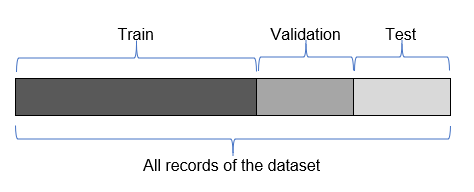
\includegraphics{img/da-split/train_test1.png}

You can also find papers with splitting only for
\texttt{train}/\texttt{test}. In this case \texttt{test} means
\texttt{validation}.

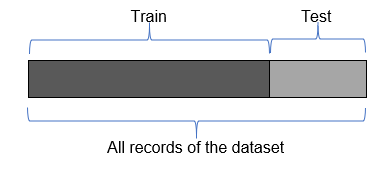
\includegraphics{img/da-split/train_test2.png}

\begin{center}\rule{0.5\linewidth}{0.5pt}\end{center}

\section{Splitting data in R}\label{splitting-data-in-r}

Lets describe some conditions before start studiyng splitting data
functions in R:

\begin{itemize}
\tightlist
\item[$\boxtimes$]
  We will use same seed for all splittings to control results
  reproduction, for example, let it be 2021.
\item[$\boxtimes$]
  We will use dataset for client churn prediction
  \texttt{Telco\ Customer\ Churn}:
  https://www.kaggle.com/blastchar/telco-customer-churn
\end{itemize}

Short dataset description:

\begin{itemize}
\tightlist
\item[$\boxtimes$]
  \texttt{customerID} - Customer ID
\item[$\boxtimes$]
  \texttt{gender} Whether the customer is a male or a female
\item[$\boxtimes$]
  \texttt{SeniorCitizen} - Whether the customer is a senior citizen or
  not (1, 0)
\item[$\boxtimes$]
  \texttt{Partner} - Whether the customer has a partner or not (Yes, No)
\item[$\boxtimes$]
  \texttt{Dependents} - Whether the customer has dependents or not (Yes,
  No)
\item[$\boxtimes$]
  \texttt{tenure} - Number of months the customer has stayed with the
  company
\item[$\boxtimes$]
  \texttt{PhoneService} - Whether the customer has a phone service or
  not (Yes, No)
\item[$\boxtimes$]
  \texttt{MultipleLines} - Whether the customer has multiple lines or
  not (Yes, No, No phone service)
\item[$\boxtimes$]
  \texttt{InternetService} - Customer's internet service provider (DSL,
  Fiber optic, No)
\item[$\boxtimes$]
  \texttt{OnlineSecurity} - Whether the customer has online security or
  not (Yes, No, No internet service)
\item[$\boxtimes$]
  \texttt{OnlineBackup} - Whether the customer has online backup or not
  (Yes, No, No internet service)
\item[$\boxtimes$]
  \texttt{DeviceProtection} - Whether the customer has device protection
  or not (Yes, No, No internet service)
\item[$\boxtimes$]
  \texttt{TechSupport} - Whether the customer has tech support or not
  (Yes, No, No internet service)
\item[$\boxtimes$]
  \texttt{StreamingTV} - Whether the customer has streaming TV or not
  (Yes, No, No internet service)
\item[$\boxtimes$]
  \texttt{StreamingMovies} - Whether the customer has streaming movies
  or not (Yes, No, No internet service)
\item[$\boxtimes$]
  \texttt{Contract} - The contract term of the customer (Month-to-month,
  One year, Two year)
\item[$\boxtimes$]
  \texttt{PaperlessBilling} - Whether the customer has paperless billing
  or not (Yes, No)
\item[$\boxtimes$]
  \texttt{PaymentMethod} - The customer's payment method (Electronic
  check, Mailed check, Bank transfer (automatic), Credit card
  (automatic))
\item[$\boxtimes$]
  \texttt{MonthlyCharges} - The amount charged to the customer monthly
\item[$\boxtimes$]
  \texttt{TotalCharges} - The total amount charged to the customer
\item[$\boxtimes$]
  \texttt{Churn} - Whether the customer churned or not (Yes or No)
\end{itemize}

\begin{Shaded}
\begin{Highlighting}[]
\CommentTok{\# read data}
\NormalTok{telecom\_users }\OtherTok{\textless{}{-}} \FunctionTok{read.csv}\NormalTok{(}\StringTok{"data/telecom\_users.csv"}\NormalTok{)}
\FunctionTok{head}\NormalTok{(telecom\_users)}
\end{Highlighting}
\end{Shaded}

A data.frame: 6 × 22

\begin{longtable}[]{@{}
  >{\raggedright\arraybackslash}p{(\columnwidth - 42\tabcolsep) * \real{0.0455}}
  >{\raggedright\arraybackslash}p{(\columnwidth - 42\tabcolsep) * \real{0.0455}}
  >{\raggedright\arraybackslash}p{(\columnwidth - 42\tabcolsep) * \real{0.0455}}
  >{\raggedright\arraybackslash}p{(\columnwidth - 42\tabcolsep) * \real{0.0455}}
  >{\raggedright\arraybackslash}p{(\columnwidth - 42\tabcolsep) * \real{0.0455}}
  >{\raggedright\arraybackslash}p{(\columnwidth - 42\tabcolsep) * \real{0.0455}}
  >{\raggedright\arraybackslash}p{(\columnwidth - 42\tabcolsep) * \real{0.0455}}
  >{\raggedright\arraybackslash}p{(\columnwidth - 42\tabcolsep) * \real{0.0455}}
  >{\raggedright\arraybackslash}p{(\columnwidth - 42\tabcolsep) * \real{0.0455}}
  >{\raggedright\arraybackslash}p{(\columnwidth - 42\tabcolsep) * \real{0.0455}}
  >{\raggedright\arraybackslash}p{(\columnwidth - 42\tabcolsep) * \real{0.0455}}
  >{\raggedright\arraybackslash}p{(\columnwidth - 42\tabcolsep) * \real{0.0455}}
  >{\raggedright\arraybackslash}p{(\columnwidth - 42\tabcolsep) * \real{0.0455}}
  >{\raggedright\arraybackslash}p{(\columnwidth - 42\tabcolsep) * \real{0.0455}}
  >{\raggedright\arraybackslash}p{(\columnwidth - 42\tabcolsep) * \real{0.0455}}
  >{\raggedright\arraybackslash}p{(\columnwidth - 42\tabcolsep) * \real{0.0455}}
  >{\raggedright\arraybackslash}p{(\columnwidth - 42\tabcolsep) * \real{0.0455}}
  >{\raggedright\arraybackslash}p{(\columnwidth - 42\tabcolsep) * \real{0.0455}}
  >{\raggedright\arraybackslash}p{(\columnwidth - 42\tabcolsep) * \real{0.0455}}
  >{\raggedright\arraybackslash}p{(\columnwidth - 42\tabcolsep) * \real{0.0455}}
  >{\raggedright\arraybackslash}p{(\columnwidth - 42\tabcolsep) * \real{0.0455}}
  >{\raggedright\arraybackslash}p{(\columnwidth - 42\tabcolsep) * \real{0.0455}}@{}}
\toprule\noalign{}
\begin{minipage}[b]{\linewidth}\raggedright
\end{minipage} & \begin{minipage}[b]{\linewidth}\raggedright
X \textless int\textgreater{}
\end{minipage} & \begin{minipage}[b]{\linewidth}\raggedright
customerID \textless chr\textgreater{}
\end{minipage} & \begin{minipage}[b]{\linewidth}\raggedright
gender \textless chr\textgreater{}
\end{minipage} & \begin{minipage}[b]{\linewidth}\raggedright
SeniorCitizen \textless int\textgreater{}
\end{minipage} & \begin{minipage}[b]{\linewidth}\raggedright
Partner \textless chr\textgreater{}
\end{minipage} & \begin{minipage}[b]{\linewidth}\raggedright
Dependents \textless chr\textgreater{}
\end{minipage} & \begin{minipage}[b]{\linewidth}\raggedright
tenure \textless int\textgreater{}
\end{minipage} & \begin{minipage}[b]{\linewidth}\raggedright
PhoneService \textless chr\textgreater{}
\end{minipage} & \begin{minipage}[b]{\linewidth}\raggedright
MultipleLines \textless chr\textgreater{}
\end{minipage} & \begin{minipage}[b]{\linewidth}\raggedright
InternetService \textless chr\textgreater{}
\end{minipage} & \begin{minipage}[b]{\linewidth}\raggedright
⋯ ⋯
\end{minipage} & \begin{minipage}[b]{\linewidth}\raggedright
DeviceProtection \textless chr\textgreater{}
\end{minipage} & \begin{minipage}[b]{\linewidth}\raggedright
TechSupport \textless chr\textgreater{}
\end{minipage} & \begin{minipage}[b]{\linewidth}\raggedright
StreamingTV \textless chr\textgreater{}
\end{minipage} & \begin{minipage}[b]{\linewidth}\raggedright
StreamingMovies \textless chr\textgreater{}
\end{minipage} & \begin{minipage}[b]{\linewidth}\raggedright
Contract \textless chr\textgreater{}
\end{minipage} & \begin{minipage}[b]{\linewidth}\raggedright
PaperlessBilling \textless chr\textgreater{}
\end{minipage} & \begin{minipage}[b]{\linewidth}\raggedright
PaymentMethod \textless chr\textgreater{}
\end{minipage} & \begin{minipage}[b]{\linewidth}\raggedright
MonthlyCharges \textless chr\textgreater{}
\end{minipage} & \begin{minipage}[b]{\linewidth}\raggedright
TotalCharges \textless dbl\textgreater{}
\end{minipage} & \begin{minipage}[b]{\linewidth}\raggedright
Churn \textless chr\textgreater{}
\end{minipage} \\
\midrule\noalign{}
\endhead
\bottomrule\noalign{}
\endlastfoot
1 & 1869 & 7010-BRBUU & Male & 0 & Yes & Yes & 72 & Yes & Yes & No & ⋯ &
No internet service & No internet service & No internet service & No
internet service & Two year & No & Credit card (automatic) & 24.1 &
1734.65 & No \\
2 & 4528 & 9688-YGXVR & Female & 0 & No & No & 44 & Yes & No & Fiber
optic & ⋯ & Yes & No & Yes & No & Month-to-month & Yes & Credit card
(automatic) & 88.15 & 3973.20 & No \\
3 & 6344 & 9286-DOJGF & Female & 1 & Yes & No & 38 & Yes & Yes & Fiber
optic & ⋯ & No & No & No & No & Month-to-month & Yes & Bank transfer
(automatic) & 74.95 & 2869.85 & Yes \\
4 & 6739 & 6994-KERXL & Male & 0 & No & No & 4 & Yes & No & DSL & ⋯ & No
& No & No & Yes & Month-to-month & Yes & Electronic check & 55.9 &
238.50 & No \\
5 & 432 & 2181-UAESM & Male & 0 & No & No & 2 & Yes & No & DSL & ⋯ & Yes
& No & No & No & Month-to-month & No & Electronic check & 53.45 & 119.50
& No \\
6 & 2215 & 4312-GVYNH & Female & 0 & Yes & No & 70 & No & No phone
service & DSL & ⋯ & Yes & Yes & No & Yes & Two year & Yes & Bank
transfer (automatic) & 49.85 & 3370.20 & No \\
\end{longtable}

Lets check the proportion of column \texttt{Churn\ ==\ Yes} and
\texttt{Churn\ ==\ No} in dataset with \texttt{CrossTable()} function
from \texttt{gmodels} package.

\begin{Shaded}
\begin{Highlighting}[]
\CommentTok{\# install.packages("gmodels")}
\end{Highlighting}
\end{Shaded}

\begin{Shaded}
\begin{Highlighting}[]
\FunctionTok{library}\NormalTok{(gmodels)}
\FunctionTok{CrossTable}\NormalTok{(telecom\_users}\SpecialCharTok{$}\NormalTok{Churn)}
\end{Highlighting}
\end{Shaded}

\begin{verbatim}

 
   Cell Contents
|-------------------------|
|                       N |
|         N / Table Total |
|-------------------------|

 
Total Observations in Table:  5986 

 
          |        No |       Yes | 
          |-----------|-----------|
          |      4399 |      1587 | 
          |     0.735 |     0.265 | 
          |-----------|-----------|



 
\end{verbatim}

You can also use \texttt{CrossTable()} to check cross proportions by
other fields. Lets check crosstable for \texttt{TechSupport} and
\texttt{Churn}:

\begin{Shaded}
\begin{Highlighting}[]
\FunctionTok{CrossTable}\NormalTok{(telecom\_users}\SpecialCharTok{$}\NormalTok{Churn, telecom\_users}\SpecialCharTok{$}\NormalTok{TechSupport) }\CommentTok{\# for example}
\end{Highlighting}
\end{Shaded}

\begin{verbatim}

 
   Cell Contents
|-------------------------|
|                       N |
| Chi-square contribution |
|           N / Row Total |
|           N / Col Total |
|         N / Table Total |
|-------------------------|

 
Total Observations in Table:  5986 

 
                    | telecom_users$TechSupport 
telecom_users$Churn |                  No | No internet service |                 Yes |           Row Total | 
--------------------|---------------------|---------------------|---------------------|---------------------|
                 No |                1738 |                1192 |                1469 |                4399 | 
                    |              87.892 |              62.377 |              29.512 |                     | 
                    |               0.395 |               0.271 |               0.334 |               0.735 | 
                    |               0.587 |               0.923 |               0.847 |                     | 
                    |               0.290 |               0.199 |               0.245 |                     | 
--------------------|---------------------|---------------------|---------------------|---------------------|
                Yes |                1222 |                  99 |                 266 |                1587 | 
                    |             243.627 |             172.904 |              81.805 |                     | 
                    |               0.770 |               0.062 |               0.168 |               0.265 | 
                    |               0.413 |               0.077 |               0.153 |                     | 
                    |               0.204 |               0.017 |               0.044 |                     | 
--------------------|---------------------|---------------------|---------------------|---------------------|
       Column Total |                2960 |                1291 |                1735 |                5986 | 
                    |               0.494 |               0.216 |               0.290 |                     | 
--------------------|---------------------|---------------------|---------------------|---------------------|

 
\end{verbatim}

You can see that most part of Churn 1222 of 1587

Next, we will check 6 possible ways to split data for train/test sets.

\begin{center}\rule{0.5\linewidth}{0.5pt}\end{center}

\subsection{\texorpdfstring{Split with
\texttt{sample()}}{Split with sample()}}\label{split-with-sample}

\begin{Shaded}
\begin{Highlighting}[]
\NormalTok{sample\_size }\OtherTok{=} \FunctionTok{round}\NormalTok{(}\FunctionTok{nrow}\NormalTok{(telecom\_users)}\SpecialCharTok{*}\NormalTok{.}\DecValTok{70}\NormalTok{) }\CommentTok{\# setting what is 70\%}
\FunctionTok{print}\NormalTok{(}\FunctionTok{paste0}\NormalTok{(}\StringTok{"Size: "}\NormalTok{, sample\_size))}

\NormalTok{index }\OtherTok{\textless{}{-}} \FunctionTok{sample}\NormalTok{(}\FunctionTok{nrow}\NormalTok{(telecom\_users), }\AttributeTok{size =}\NormalTok{ sample\_size)}
 
\NormalTok{train }\OtherTok{\textless{}{-}}\NormalTok{ telecom\_users[index, ] }\CommentTok{\# index is numbers of selected rows from dataset}
\NormalTok{test }\OtherTok{\textless{}{-}}\NormalTok{telecom\_users[}\SpecialCharTok{{-}}\NormalTok{index, ] }\CommentTok{\# {-}index select only rows not in index}
\end{Highlighting}
\end{Shaded}

\begin{verbatim}
[1] "Size: 4190"
\end{verbatim}

\begin{Shaded}
\begin{Highlighting}[]
\CommentTok{\# check Churn == Yes/No proportion in train/test}
\FunctionTok{CrossTable}\NormalTok{(train}\SpecialCharTok{$}\NormalTok{Churn)}
\end{Highlighting}
\end{Shaded}

\begin{verbatim}

 
   Cell Contents
|-------------------------|
|                       N |
|         N / Table Total |
|-------------------------|

 
Total Observations in Table:  4190 

 
          |        No |       Yes | 
          |-----------|-----------|
          |      3074 |      1116 | 
          |     0.734 |     0.266 | 
          |-----------|-----------|



 
\end{verbatim}

\begin{Shaded}
\begin{Highlighting}[]
\CommentTok{\# check Churn == Yes/No proportion in train/test}
\FunctionTok{CrossTable}\NormalTok{(test}\SpecialCharTok{$}\NormalTok{Churn)}
\end{Highlighting}
\end{Shaded}

\begin{verbatim}

 
   Cell Contents
|-------------------------|
|                       N |
|         N / Table Total |
|-------------------------|

 
Total Observations in Table:  1796 

 
          |        No |       Yes | 
          |-----------|-----------|
          |      1325 |       471 | 
          |     0.738 |     0.262 | 
          |-----------|-----------|



 
\end{verbatim}

Its 0.260 for train and 0.276 for test. Diffrence is 1,6\%, so, its
close.

\begin{center}\rule{0.5\linewidth}{0.5pt}\end{center}

\subsection{\texorpdfstring{Split with \texttt{sample\_frac} from
\texttt{dplyr}}{Split with sample\_frac from dplyr}}\label{split-with-sample_frac-from-dplyr}

\begin{Shaded}
\begin{Highlighting}[]
\FunctionTok{library}\NormalTok{(dplyr)}
\FunctionTok{set.seed}\NormalTok{(}\DecValTok{2023}\NormalTok{)}

\CommentTok{\# Using the above function to create 70 {-} 30 slipt into test and train}

\NormalTok{tu }\OtherTok{\textless{}{-}}\NormalTok{ telecom\_users }\SpecialCharTok{\%\textgreater{}\%} \FunctionTok{mutate}\NormalTok{(}\AttributeTok{Id =} \FunctionTok{row\_number}\NormalTok{())}

\NormalTok{train }\OtherTok{\textless{}{-}}\NormalTok{ tu }\SpecialCharTok{\%\textgreater{}\%} \FunctionTok{sample\_frac}\NormalTok{(.}\DecValTok{70}\NormalTok{)}
\NormalTok{test }\OtherTok{\textless{}{-}}\NormalTok{ tu[}\SpecialCharTok{{-}}\NormalTok{train}\SpecialCharTok{$}\NormalTok{Id, ]}
\end{Highlighting}
\end{Shaded}

\begin{verbatim}

Attaching package: 'dplyr'


The following objects are masked from 'package:stats':

    filter, lag


The following objects are masked from 'package:base':

    intersect, setdiff, setequal, union

\end{verbatim}

\begin{Shaded}
\begin{Highlighting}[]
\FunctionTok{nrow}\NormalTok{(train)}
\end{Highlighting}
\end{Shaded}

4190

\begin{Shaded}
\begin{Highlighting}[]
\CommentTok{\# check Churn == Yes/No proportion in train/test}
\FunctionTok{CrossTable}\NormalTok{(train}\SpecialCharTok{$}\NormalTok{Churn)}
\FunctionTok{CrossTable}\NormalTok{(test}\SpecialCharTok{$}\NormalTok{Churn)}
\end{Highlighting}
\end{Shaded}

\begin{verbatim}

 
   Cell Contents
|-------------------------|
|                       N |
|         N / Table Total |
|-------------------------|

 
Total Observations in Table:  4190 

 
          |        No |       Yes | 
          |-----------|-----------|
          |      3099 |      1091 | 
          |     0.740 |     0.260 | 
          |-----------|-----------|



 

 
   Cell Contents
|-------------------------|
|                       N |
|         N / Table Total |
|-------------------------|

 
Total Observations in Table:  1796 

 
          |        No |       Yes | 
          |-----------|-----------|
          |      1300 |       496 | 
          |     0.724 |     0.276 | 
          |-----------|-----------|



 
\end{verbatim}

\texttt{sample\_n} made other proportion of \texttt{Churn\ ==\ Yes/No}
and difference just 0.7\%.

\begin{center}\rule{0.5\linewidth}{0.5pt}\end{center}

\subsection{\texorpdfstring{Split with \texttt{createDataPartition()}
from
\texttt{caret}}{Split with createDataPartition() from caret}}\label{split-with-createdatapartition-from-caret}

\begin{Shaded}
\begin{Highlighting}[]
\CommentTok{\#install.packages("caret")}
\end{Highlighting}
\end{Shaded}

\begin{verbatim}
Updating HTML index of packages in '.Library'

Making 'packages.html' ...
 done
\end{verbatim}

\begin{Shaded}
\begin{Highlighting}[]
\FunctionTok{library}\NormalTok{(caret)}
\FunctionTok{set.seed}\NormalTok{(}\DecValTok{2023}\NormalTok{)}
 
\NormalTok{index }\OtherTok{=} \FunctionTok{createDataPartition}\NormalTok{(telecom\_users}\SpecialCharTok{$}\NormalTok{Churn, }\AttributeTok{p =} \FloatTok{0.70}\NormalTok{, }\AttributeTok{list =} \ConstantTok{FALSE}\NormalTok{)}
\NormalTok{train }\OtherTok{=}\NormalTok{ telecom\_users[index, ]}
\NormalTok{test }\OtherTok{=}\NormalTok{ telecom\_users[}\SpecialCharTok{{-}}\NormalTok{index, ]}
\end{Highlighting}
\end{Shaded}

\begin{verbatim}
Loading required package: ggplot2

Loading required package: lattice
\end{verbatim}

\begin{Shaded}
\begin{Highlighting}[]
\CommentTok{\# check Churn == Yes/No proportion in train/test}
\FunctionTok{CrossTable}\NormalTok{(train}\SpecialCharTok{$}\NormalTok{Churn)}
\FunctionTok{CrossTable}\NormalTok{(test}\SpecialCharTok{$}\NormalTok{Churn)}
\end{Highlighting}
\end{Shaded}

\begin{verbatim}

 
   Cell Contents
|-------------------------|
|                       N |
|         N / Table Total |
|-------------------------|

 
Total Observations in Table:  4191 

 
          |        No |       Yes | 
          |-----------|-----------|
          |      3080 |      1111 | 
          |     0.735 |     0.265 | 
          |-----------|-----------|



 

 
   Cell Contents
|-------------------------|
|                       N |
|         N / Table Total |
|-------------------------|

 
Total Observations in Table:  1795 

 
          |        No |       Yes | 
          |-----------|-----------|
          |      1319 |       476 | 
          |     0.735 |     0.265 | 
          |-----------|-----------|



 
\end{verbatim}

Ckeck the proportion of target variable. Caret trying to make the same
split for both train and test. This is one of the best split methods in
R.

\begin{center}\rule{0.5\linewidth}{0.5pt}\end{center}

\subsection{\texorpdfstring{Split with \texttt{sample.split} from
\texttt{caTools}}{Split with sample.split from caTools}}\label{split-with-sample.split-from-catools}

\begin{Shaded}
\begin{Highlighting}[]
\CommentTok{\#install.packages("caTools")}
\end{Highlighting}
\end{Shaded}

\begin{Shaded}
\begin{Highlighting}[]
\FunctionTok{library}\NormalTok{(caTools)}
 
\FunctionTok{set.seed}\NormalTok{(}\DecValTok{2023}\NormalTok{)}
\NormalTok{sample }\OtherTok{=} \FunctionTok{sample.split}\NormalTok{(telecom\_users}\SpecialCharTok{$}\NormalTok{Churn, }\AttributeTok{SplitRatio =}\NormalTok{ .}\DecValTok{70}\NormalTok{)}

\NormalTok{train }\OtherTok{=}\NormalTok{ telecom\_users[sample, ]}
\NormalTok{test  }\OtherTok{=}\NormalTok{ telecom\_users[}\SpecialCharTok{!}\NormalTok{sample, ]}
\end{Highlighting}
\end{Shaded}

\begin{Shaded}
\begin{Highlighting}[]
\CommentTok{\# check Churn == Yes/No proportion in train/test}
\FunctionTok{CrossTable}\NormalTok{(train}\SpecialCharTok{$}\NormalTok{Churn)}
\FunctionTok{CrossTable}\NormalTok{(test}\SpecialCharTok{$}\NormalTok{Churn)}
\end{Highlighting}
\end{Shaded}

\begin{verbatim}

 
   Cell Contents
|-------------------------|
|                       N |
|         N / Table Total |
|-------------------------|

 
Total Observations in Table:  4190 

 
          |        No |       Yes | 
          |-----------|-----------|
          |      3079 |      1111 | 
          |     0.735 |     0.265 | 
          |-----------|-----------|



 

 
   Cell Contents
|-------------------------|
|                       N |
|         N / Table Total |
|-------------------------|

 
Total Observations in Table:  1796 

 
          |        No |       Yes | 
          |-----------|-----------|
          |      1320 |       476 | 
          |     0.735 |     0.265 | 
          |-----------|-----------|



 
\end{verbatim}

\begin{center}\rule{0.5\linewidth}{0.5pt}\end{center}

Для нашого курсу це не потрібно поки! Переходимо до наступної теми. Цей
матеріал в детелях буде розглянуто під час вивчення крос-валідації.

\section{Splitting for n-folds}\label{splitting-for-n-folds}

\begin{Shaded}
\begin{Highlighting}[]
\CommentTok{\# read data again}
\FunctionTok{library}\NormalTok{(caret)}
\NormalTok{telecom\_users }\OtherTok{\textless{}{-}} \FunctionTok{read.csv}\NormalTok{(}\StringTok{"../../data/telecom\_users.csv"}\NormalTok{)}
\FunctionTok{nrow}\NormalTok{(telecom\_users)}
\FunctionTok{head}\NormalTok{(telecom\_users)}
\end{Highlighting}
\end{Shaded}

5986

A data.frame: 6 × 22

\begin{longtable}[]{@{}
  >{\raggedright\arraybackslash}p{(\columnwidth - 42\tabcolsep) * \real{0.0455}}
  >{\raggedright\arraybackslash}p{(\columnwidth - 42\tabcolsep) * \real{0.0455}}
  >{\raggedright\arraybackslash}p{(\columnwidth - 42\tabcolsep) * \real{0.0455}}
  >{\raggedright\arraybackslash}p{(\columnwidth - 42\tabcolsep) * \real{0.0455}}
  >{\raggedright\arraybackslash}p{(\columnwidth - 42\tabcolsep) * \real{0.0455}}
  >{\raggedright\arraybackslash}p{(\columnwidth - 42\tabcolsep) * \real{0.0455}}
  >{\raggedright\arraybackslash}p{(\columnwidth - 42\tabcolsep) * \real{0.0455}}
  >{\raggedright\arraybackslash}p{(\columnwidth - 42\tabcolsep) * \real{0.0455}}
  >{\raggedright\arraybackslash}p{(\columnwidth - 42\tabcolsep) * \real{0.0455}}
  >{\raggedright\arraybackslash}p{(\columnwidth - 42\tabcolsep) * \real{0.0455}}
  >{\raggedright\arraybackslash}p{(\columnwidth - 42\tabcolsep) * \real{0.0455}}
  >{\raggedright\arraybackslash}p{(\columnwidth - 42\tabcolsep) * \real{0.0455}}
  >{\raggedright\arraybackslash}p{(\columnwidth - 42\tabcolsep) * \real{0.0455}}
  >{\raggedright\arraybackslash}p{(\columnwidth - 42\tabcolsep) * \real{0.0455}}
  >{\raggedright\arraybackslash}p{(\columnwidth - 42\tabcolsep) * \real{0.0455}}
  >{\raggedright\arraybackslash}p{(\columnwidth - 42\tabcolsep) * \real{0.0455}}
  >{\raggedright\arraybackslash}p{(\columnwidth - 42\tabcolsep) * \real{0.0455}}
  >{\raggedright\arraybackslash}p{(\columnwidth - 42\tabcolsep) * \real{0.0455}}
  >{\raggedright\arraybackslash}p{(\columnwidth - 42\tabcolsep) * \real{0.0455}}
  >{\raggedright\arraybackslash}p{(\columnwidth - 42\tabcolsep) * \real{0.0455}}
  >{\raggedright\arraybackslash}p{(\columnwidth - 42\tabcolsep) * \real{0.0455}}
  >{\raggedright\arraybackslash}p{(\columnwidth - 42\tabcolsep) * \real{0.0455}}@{}}
\toprule\noalign{}
\begin{minipage}[b]{\linewidth}\raggedright
\end{minipage} & \begin{minipage}[b]{\linewidth}\raggedright
X \textless int\textgreater{}
\end{minipage} & \begin{minipage}[b]{\linewidth}\raggedright
customerID \textless chr\textgreater{}
\end{minipage} & \begin{minipage}[b]{\linewidth}\raggedright
gender \textless chr\textgreater{}
\end{minipage} & \begin{minipage}[b]{\linewidth}\raggedright
SeniorCitizen \textless int\textgreater{}
\end{minipage} & \begin{minipage}[b]{\linewidth}\raggedright
Partner \textless chr\textgreater{}
\end{minipage} & \begin{minipage}[b]{\linewidth}\raggedright
Dependents \textless chr\textgreater{}
\end{minipage} & \begin{minipage}[b]{\linewidth}\raggedright
tenure \textless int\textgreater{}
\end{minipage} & \begin{minipage}[b]{\linewidth}\raggedright
PhoneService \textless chr\textgreater{}
\end{minipage} & \begin{minipage}[b]{\linewidth}\raggedright
MultipleLines \textless chr\textgreater{}
\end{minipage} & \begin{minipage}[b]{\linewidth}\raggedright
InternetService \textless chr\textgreater{}
\end{minipage} & \begin{minipage}[b]{\linewidth}\raggedright
\ldots{} \ldots{}
\end{minipage} & \begin{minipage}[b]{\linewidth}\raggedright
DeviceProtection \textless chr\textgreater{}
\end{minipage} & \begin{minipage}[b]{\linewidth}\raggedright
TechSupport \textless chr\textgreater{}
\end{minipage} & \begin{minipage}[b]{\linewidth}\raggedright
StreamingTV \textless chr\textgreater{}
\end{minipage} & \begin{minipage}[b]{\linewidth}\raggedright
StreamingMovies \textless chr\textgreater{}
\end{minipage} & \begin{minipage}[b]{\linewidth}\raggedright
Contract \textless chr\textgreater{}
\end{minipage} & \begin{minipage}[b]{\linewidth}\raggedright
PaperlessBilling \textless chr\textgreater{}
\end{minipage} & \begin{minipage}[b]{\linewidth}\raggedright
PaymentMethod \textless chr\textgreater{}
\end{minipage} & \begin{minipage}[b]{\linewidth}\raggedright
MonthlyCharges \textless chr\textgreater{}
\end{minipage} & \begin{minipage}[b]{\linewidth}\raggedright
TotalCharges \textless dbl\textgreater{}
\end{minipage} & \begin{minipage}[b]{\linewidth}\raggedright
Churn \textless chr\textgreater{}
\end{minipage} \\
\midrule\noalign{}
\endhead
\bottomrule\noalign{}
\endlastfoot
1 & 1869 & 7010-BRBUU & Male & 0 & Yes & Yes & 72 & Yes & Yes & No &
\ldots{} & No internet service & No internet service & No internet
service & No internet service & Two year & No & Credit card (automatic)
& 24.1 & 1734.65 & No \\
2 & 4528 & 9688-YGXVR & Female & 0 & No & No & 44 & Yes & No & Fiber
optic & \ldots{} & Yes & No & Yes & No & Month-to-month & Yes & Credit
card (automatic) & 88.15 & 3973.20 & No \\
3 & 6344 & 9286-DOJGF & Female & 1 & Yes & No & 38 & Yes & Yes & Fiber
optic & \ldots{} & No & No & No & No & Month-to-month & Yes & Bank
transfer (automatic) & 74.95 & 2869.85 & Yes \\
4 & 6739 & 6994-KERXL & Male & 0 & No & No & 4 & Yes & No & DSL &
\ldots{} & No & No & No & Yes & Month-to-month & Yes & Electronic check
& 55.9 & 238.50 & No \\
5 & 432 & 2181-UAESM & Male & 0 & No & No & 2 & Yes & No & DSL &
\ldots{} & Yes & No & No & No & Month-to-month & No & Electronic check &
53.45 & 119.50 & No \\
6 & 2215 & 4312-GVYNH & Female & 0 & Yes & No & 70 & No & No phone
service & DSL & \ldots{} & Yes & Yes & No & Yes & Two year & Yes & Bank
transfer (automatic) & 49.85 & 3370.20 & No \\
\end{longtable}

\begin{Shaded}
\begin{Highlighting}[]
\NormalTok{folds }\OtherTok{\textless{}{-}} \FunctionTok{createFolds}\NormalTok{(telecom\_users)}
\NormalTok{folds}
\end{Highlighting}
\end{Shaded}

\begin{description}
\tightlist
\item[\$Fold01]
\begin{enumerate}
\def\labelenumi{\arabic{enumi}.}
\tightlist
\item[]
\item
  1
\item
  10
\end{enumerate}
\item[\$Fold02]
\begin{enumerate}
\def\labelenumi{\arabic{enumi}.}
\tightlist
\item[]
\item
  3
\item
  4
\item
  15
\end{enumerate}
\item[\$Fold03]
\begin{enumerate}
\def\labelenumi{\arabic{enumi}.}
\tightlist
\item[]
\item
  2
\item
  17
\end{enumerate}
\item[\$Fold04]
8 \$Fold05

\begin{enumerate}
\def\labelenumi{\arabic{enumi}.}
\tightlist
\item
  16
\item
  22
\end{enumerate}
\item[\$Fold06]
\begin{enumerate}
\def\labelenumi{\arabic{enumi}.}
\tightlist
\item[]
\item
  9
\item
  18
\end{enumerate}
\item[\$Fold07]
\begin{enumerate}
\def\labelenumi{\arabic{enumi}.}
\tightlist
\item[]
\item
  19
\item
  20
\end{enumerate}
\item[\$Fold08]
\begin{enumerate}
\def\labelenumi{\arabic{enumi}.}
\tightlist
\item[]
\item
  5
\item
  12
\item
  14
\end{enumerate}
\item[\$Fold09]
11 \$Fold10

\begin{enumerate}
\def\labelenumi{\arabic{enumi}.}
\tightlist
\item
  6
\item
  7
\item
  13
\item
  21
\end{enumerate}
\end{description}

\begin{Shaded}
\begin{Highlighting}[]
\CommentTok{\#library(caret)}
\CommentTok{\#library(mlbench)}
\CommentTok{\#data(Sonar)}
 
\CommentTok{\#folds \textless{}{-} createFolds(Sonar$Class)}
\CommentTok{\#str(folds)}
\end{Highlighting}
\end{Shaded}

\begin{center}\rule{0.5\linewidth}{0.5pt}\end{center}

\section{References}\label{references-8}

\begin{enumerate}
\def\labelenumi{\arabic{enumi}.}
\tightlist
\item
  About Train, Validation and Test Sets in Machine Learning by Tarang
  Shah. Url:
  https://towardsdatascience.com/train-validation-and-test-sets-72cb40cba9e7
\end{enumerate}

\part{ТЕМА 7. ОГЛЯДОВИЙ АНАЛІЗ ДАНИХ}

\chapter{EDA на прикладі
вина}\label{eda-ux43dux430-ux43fux440ux438ux43aux43bux430ux434ux456-ux432ux438ux43dux430}

https://github.com/Ashish25/EDA\_Rmd/blob/master/MyWhiteWine.Rmd

https://www.knowledgehut.com/blog/data-science/eda-data-science

\section{Етапи дослідницького аналізу даних (Exploratory Data
Analysis)}\label{ux435ux442ux430ux43fux438-ux434ux43eux441ux43bux456ux434ux43dux438ux446ux44cux43aux43eux433ux43e-ux430ux43dux430ux43bux456ux437ux443-ux434ux430ux43dux438ux445-exploratory-data-analysis}

\begin{itemize}
\tightlist
\item
  \textbf{Збір даних}з Збір та об'єднання всіх необхідних даних для
  аналіз у2. **Очищення даних*в: Видалення або виправлення помилок,
  пропущених значень та аномалій у дан и
\end{itemize}

\begin{enumerate}
\def\labelenumi{\arabic{enumi}.}
\setcounter{enumi}{2}
\tightlist
\item
  **Описова статистикао*: Обчислення основних статистичних показників,
  таких як середнє, медіана, мода, стандартне відхилення т о
\item
  \textbf{Візуалізація данис}: Створення графіків та діаграм для
  виявлення закономірностей, трендів та взаємозв'язків у д а.
\item
  \textbf{Виявлення взаємозв'язкав}: Аналіз кореляцій та інших
  статистичних взаємозв'язків між змі ни.
\item
  \textbf{Формулювання гіповез}: Висування гіпотез на основі виявлених
  закономірностей та взаємозв 'ів.
\item
  \textbf{Перевірка гіпвтез}: Використання статистичних методів для
  перевірки висунутих гтез.
\item
  \textbf{Інтерпретація резульаатів}: Аналіз отриманих результатів та
  формулювання в и вків.
\item
  \textbf{Документдвання}: Документування всіх етапів аналізу, включаючи
  проблеми, рішення та висновки.
\end{enumerate}

Оволодіння дослідницьким аналізом даних (EDA) є важливим для розуміння
ваших даних, виявлення закономірностей та отримання інсайтів, які можуть
інформувати подальший аналіз або прийняття рішень. Дані є життєво
важливими для передових груп, і здатність витягувати інсайти з даних
стала важливим навиком у сучасному світі, орієнтованому на статистику.
Дослідницький аналіз даних (EDA) є потужним методом, який дозволяє
аналітикам, вченим та дослідникам отримати повне уявлення про свої дані
до початку формального моделювання або тестування гіпотез.

Це ітеративний процес, який включає узагальнення, візуалізацію та
дослідження інформації для виявлення закономірностей, аномалій та
взаємозв'язків, які можуть бути неочевидними на перший погляд. У цій
статті ми зрозуміємо та реалізуємо критичні кроки для виконання
дослідницького аналізу даних. Ось кроки, які допоможуть вам оволодіти
EDA:

\section{Кроки для оволодіння дослідницьким аналізом
даних}\label{ux43aux440ux43eux43aux438-ux434ux43bux44f-ux43eux432ux43eux43bux43eux434ux456ux43dux43dux44f-ux434ux43eux441ux43bux456ux434ux43dux438ux446ux44cux43aux438ux43c-ux430ux43dux430ux43bux456ux437ux43eux43c-ux434ux430ux43dux438ux445}

\textbf{Крок 1:} Зрозумійте проблему та дані\\
\textbf{Крок 2:} Імпортуйте та перевірте дані\\
\textbf{Крок 3:} Обробка пропущених значень\\
\textbf{Крок 4:} Дослідження характеристик даних\\
\textbf{Крок 5:} Виконання трансформації даних\\
\textbf{Крок 6:} Візуалізація взаємозв'язків даних\\
\textbf{Крок 7:} Обробка викидів\\
\textbf{Крок 8:} Комунікація висновків та інсайтів

\subsection{Мета цього
проекту}\label{ux43cux435ux442ux430-ux446ux44cux43eux433ux43e-ux43fux440ux43eux435ux43aux442ux443}

У цьому проекті ми будемо аналізувати дані про біле вино і намагатися
зрозуміти, які змінні відповідають за якість вина. Спочатку ми спробуємо
отримати уявлення про змінні самі по собі, а потім спробуємо знайти
кореляцію між ними та якістю вина з урахуванням інших факторів.

\begin{Shaded}
\begin{Highlighting}[]
\CommentTok{\#install.packages("GGally")}
\end{Highlighting}
\end{Shaded}

\begin{Shaded}
\begin{Highlighting}[]
\FunctionTok{library}\NormalTok{(ggplot2)}
\FunctionTok{library}\NormalTok{(RColorBrewer)}
\FunctionTok{library}\NormalTok{(GGally)}
\end{Highlighting}
\end{Shaded}

\begin{Shaded}
\begin{Highlighting}[]
\NormalTok{white\_wines }\OtherTok{\textless{}{-}} \FunctionTok{read.csv}\NormalTok{(}\StringTok{\textquotesingle{}https://raw.githubusercontent.com/Ashish25/EDA\_Rmd/refs/heads/master/wineQualityWhites.csv\textquotesingle{}}\NormalTok{, }
                        \AttributeTok{header =} \ConstantTok{TRUE}\NormalTok{, }
                        \AttributeTok{sep =} \StringTok{\textquotesingle{},\textquotesingle{}}\NormalTok{, }
                        \AttributeTok{row.names =} \DecValTok{1}\NormalTok{)}
\end{Highlighting}
\end{Shaded}

\subsection{Контекст}\label{ux43aux43eux43dux442ux435ux43aux441ux442}

Два набори даних стосуються червоних і білих варіантів португальського
вина ``Vinho Verde''. Для отримання додаткової інформації зверніться до
посилання {[}Cortez et al., 2009{]}. Через питання конфіденційності та
логістики доступні лише фізико-хімічні (вхідні) та сенсорні (вихідні)
змінні (наприклад, немає даних про типи винограду, бренд вина, ціну
продажу вина тощо).

Ці набори даних можна розглядати як завдання класифікації або регресії.
Класи впорядковані і не збалансовані (наприклад, набагато більше
звичайних вин, ніж відмінних або поганих).

Цей набір даних також доступний у репозиторії машинного навчання UCI:
https://archive.ics.uci.edu/ml/datasets/wine+quality.

\subsection{Опис}\label{ux43eux43fux438ux441}

Для отримання додаткової інформації читайте {[}Cortez et al., 2009{]}.

Вхідні змінні (на основі фізико-хімічних тестів): 1. \textbf{fixed
acidity} - фіксована кислотність 2. \textbf{volatile acidity} - летка
кислотність 3. \textbf{citric acid} - лимонна кислота 4.
\textbf{residual sugar} - залишковий цукор 5. \textbf{chlorides} -
хлориди 6. \textbf{free sulfur dioxide} - вільний діоксид сірки 7.
\textbf{total sulfur dioxide} - загальний діоксид сірки 8.
\textbf{density} - густина 9. \textbf{pH} - рівень pH 10.
\textbf{sulphates} - сульфати 11. \textbf{alcohol} - вміст алкоголю

Вихідна змінна (на основі сенсорних даних): 12. \textbf{quality} -
якість (оцінка від 0 до 10)

\subsection{Перший
погляд}\label{ux43fux435ux440ux448ux438ux439-ux43fux43eux433ux43bux44fux434}

Ми маємо наступні змінні:

\begin{Shaded}
\begin{Highlighting}[]
\FunctionTok{names}\NormalTok{(white\_wines)}
\end{Highlighting}
\end{Shaded}

\begin{enumerate}
\def\labelenumi{\arabic{enumi}.}
\tightlist
\item
  `fixed.acidity'
\item
  `volatile.acidity'
\item
  `citric.acid'
\item
  `residual.sugar'
\item
  `chlorides'
\item
  `free.sulfur.dioxide'
\item
  `total.sulfur.dioxide'
\item
  `density'
\item
  `pH'
\item
  `sulphates'
\item
  `alcohol'
\item
  `quality'
\end{enumerate}

\begin{Shaded}
\begin{Highlighting}[]
\FunctionTok{str}\NormalTok{(white\_wines)}
\end{Highlighting}
\end{Shaded}

\begin{verbatim}
'data.frame':   4898 obs. of  12 variables:
 $ fixed.acidity       : num  7 6.3 8.1 7.2 7.2 8.1 6.2 7 6.3 8.1 ...
 $ volatile.acidity    : num  0.27 0.3 0.28 0.23 0.23 0.28 0.32 0.27 0.3 0.22 ...
 $ citric.acid         : num  0.36 0.34 0.4 0.32 0.32 0.4 0.16 0.36 0.34 0.43 ...
 $ residual.sugar      : num  20.7 1.6 6.9 8.5 8.5 6.9 7 20.7 1.6 1.5 ...
 $ chlorides           : num  0.045 0.049 0.05 0.058 0.058 0.05 0.045 0.045 0.049 0.044 ...
 $ free.sulfur.dioxide : num  45 14 30 47 47 30 30 45 14 28 ...
 $ total.sulfur.dioxide: num  170 132 97 186 186 97 136 170 132 129 ...
 $ density             : num  1.001 0.994 0.995 0.996 0.996 ...
 $ pH                  : num  3 3.3 3.26 3.19 3.19 3.26 3.18 3 3.3 3.22 ...
 $ sulphates           : num  0.45 0.49 0.44 0.4 0.4 0.44 0.47 0.45 0.49 0.45 ...
 $ alcohol             : num  8.8 9.5 10.1 9.9 9.9 10.1 9.6 8.8 9.5 11 ...
 $ quality             : int  6 6 6 6 6 6 6 6 6 6 ...
\end{verbatim}

\begin{Shaded}
\begin{Highlighting}[]
\FunctionTok{summary}\NormalTok{(white\_wines)}
\end{Highlighting}
\end{Shaded}

\begin{verbatim}
 fixed.acidity    volatile.acidity  citric.acid     residual.sugar  
 Min.   : 3.800   Min.   :0.0800   Min.   :0.0000   Min.   : 0.600  
 1st Qu.: 6.300   1st Qu.:0.2100   1st Qu.:0.2700   1st Qu.: 1.700  
 Median : 6.800   Median :0.2600   Median :0.3200   Median : 5.200  
 Mean   : 6.855   Mean   :0.2782   Mean   :0.3342   Mean   : 6.391  
 3rd Qu.: 7.300   3rd Qu.:0.3200   3rd Qu.:0.3900   3rd Qu.: 9.900  
 Max.   :14.200   Max.   :1.1000   Max.   :1.6600   Max.   :65.800  
   chlorides       free.sulfur.dioxide total.sulfur.dioxide    density      
 Min.   :0.00900   Min.   :  2.00      Min.   :  9.0        Min.   :0.9871  
 1st Qu.:0.03600   1st Qu.: 23.00      1st Qu.:108.0        1st Qu.:0.9917  
 Median :0.04300   Median : 34.00      Median :134.0        Median :0.9937  
 Mean   :0.04577   Mean   : 35.31      Mean   :138.4        Mean   :0.9940  
 3rd Qu.:0.05000   3rd Qu.: 46.00      3rd Qu.:167.0        3rd Qu.:0.9961  
 Max.   :0.34600   Max.   :289.00      Max.   :440.0        Max.   :1.0390  
       pH          sulphates         alcohol         quality     
 Min.   :2.720   Min.   :0.2200   Min.   : 8.00   Min.   :3.000  
 1st Qu.:3.090   1st Qu.:0.4100   1st Qu.: 9.50   1st Qu.:5.000  
 Median :3.180   Median :0.4700   Median :10.40   Median :6.000  
 Mean   :3.188   Mean   :0.4898   Mean   :10.51   Mean   :5.878  
 3rd Qu.:3.280   3rd Qu.:0.5500   3rd Qu.:11.40   3rd Qu.:6.000  
 Max.   :3.820   Max.   :1.0800   Max.   :14.20   Max.   :9.000  
\end{verbatim}

\subsection{Підсумок}\label{ux43fux456ux434ux441ux443ux43cux43eux43a}

Підсумок показує, що максимальні значення для змінних \textbf{residual
sugar} (залишковий цукор), \textbf{chlorides} (хлориди) та \textbf{free
sulfur dioxide} (вільний діоксид сірки) значно відрізняються від інших
значень. Це можуть бути викиди або проблеми з введенням даних, або ж це
можуть бути дійсно особливі вина.

\section{Одновимірні
графіки}\label{ux43eux434ux43dux43eux432ux438ux43cux456ux440ux43dux456-ux433ux440ux430ux444ux456ux43aux438}

Давайте побудуємо розподіл кожної змінної, оскільки я хочу спочатку
отримати уявлення про змінні. Виходячи з форми розподілу, тобто
нормального, позитивного або негативного перекосу, і кількості викидів,
це також допоможе нам зрозуміти, чого очікувати, коли я буду будувати
графіки різних змінних одна проти одної.

\subsection{Якість
(Quality)}\label{ux44fux43aux456ux441ux442ux44c-quality}

Оскільки якість є числовою змінною, ми додамо її як фактор.

\begin{Shaded}
\begin{Highlighting}[]
\NormalTok{white\_wines}\SpecialCharTok{$}\NormalTok{quality.lvl}\OtherTok{=}\FunctionTok{cut}\NormalTok{(white\_wines}\SpecialCharTok{$}\NormalTok{quality, }
                          \FunctionTok{c}\NormalTok{(}\DecValTok{0}\NormalTok{,}\DecValTok{1}\NormalTok{,}\DecValTok{2}\NormalTok{,}\DecValTok{3}\NormalTok{,}\DecValTok{4}\NormalTok{,}\DecValTok{5}\NormalTok{,}\DecValTok{6}\NormalTok{,}\DecValTok{7}\NormalTok{,}\DecValTok{8}\NormalTok{,}\DecValTok{9}\NormalTok{,}\DecValTok{10}\NormalTok{), }
                          \AttributeTok{labels =} \FunctionTok{c}\NormalTok{(}\DecValTok{1}\NormalTok{,}\DecValTok{2}\NormalTok{,}\DecValTok{3}\NormalTok{,}\DecValTok{4}\NormalTok{,}\DecValTok{5}\NormalTok{,}\DecValTok{6}\NormalTok{,}\DecValTok{7}\NormalTok{,}\DecValTok{8}\NormalTok{,}\DecValTok{9}\NormalTok{,}\DecValTok{10}\NormalTok{))}

\FunctionTok{ggplot}\NormalTok{(}\FunctionTok{aes}\NormalTok{(}\AttributeTok{x =}\NormalTok{ quality.lvl, }\AttributeTok{fill =} \FunctionTok{after\_stat}\NormalTok{(count)), }\AttributeTok{data =}\NormalTok{ white\_wines) }\SpecialCharTok{+}
  \FunctionTok{geom\_bar}\NormalTok{() }\SpecialCharTok{+}
  \FunctionTok{scale\_x\_discrete}\NormalTok{()}
\end{Highlighting}
\end{Shaded}

\includegraphics[width=4.375in,height=4.375in]{eda_files/figure-pdf/cell-8-output-1.png}

Схоже на нормальний розподіл. Більшість вин мають якість близько 5/6/7.
Оскільки вина хорошої та поганої якості майже як викиди, може бути важко
отримати точну модель якості вина. Давайте подивимося на інші графіки.

\begin{center}\rule{0.5\linewidth}{0.5pt}\end{center}

\subsection{Алкоголь
(Alcohol)}\label{ux430ux43bux43aux43eux433ux43eux43bux44c-alcohol}

Давайте перевіримо розподіл алкоголю.

\begin{Shaded}
\begin{Highlighting}[]
\FunctionTok{ggplot}\NormalTok{(}\FunctionTok{aes}\NormalTok{(}\AttributeTok{x =}\NormalTok{ alcohol, }\AttributeTok{fill =}\NormalTok{ ..count..), }\AttributeTok{data =}\NormalTok{ white\_wines) }\SpecialCharTok{+}
  \FunctionTok{geom\_histogram}\NormalTok{(}\AttributeTok{binwidth =} \FloatTok{0.1}\NormalTok{) }\SpecialCharTok{+}
  \FunctionTok{scale\_fill\_gradient}\NormalTok{(}\AttributeTok{low =} \StringTok{"\#fcf4d9"}\NormalTok{, }\AttributeTok{high =} \StringTok{"\#f9ae00"}\NormalTok{)}
\end{Highlighting}
\end{Shaded}

\includegraphics[width=4.375in,height=4.375in]{eda_files/figure-pdf/cell-9-output-1.png}

Набагато більш різнорідний, але ми маємо гарний пік близько 9,5\% за
об'ємом. Загалом, це все ще виглядає як нормальний розподіл, з невеликим
перекосом вліво.

\subsection{Залишковий цукор (Residual
Sugar)}\label{ux437ux430ux43bux438ux448ux43aux43eux432ux438ux439-ux446ux443ux43aux43eux440-residual-sugar}

Залишковий цукор - це кількість цукру, що залишилася після ферментації.

\begin{Shaded}
\begin{Highlighting}[]
\NormalTok{gridExtra}\SpecialCharTok{::} \FunctionTok{grid.arrange}\NormalTok{(}\FunctionTok{ggplot}\NormalTok{(white\_wines, }\FunctionTok{aes}\NormalTok{( }\AttributeTok{x =} \DecValTok{1}\NormalTok{, }\AttributeTok{y =}\NormalTok{ residual.sugar ) ) }\SpecialCharTok{+} 
               \FunctionTok{geom\_jitter}\NormalTok{(}\AttributeTok{color =} \StringTok{\textquotesingle{}blue\textquotesingle{}}\NormalTok{, }\AttributeTok{size =} \FloatTok{0.2}\NormalTok{, }\AttributeTok{alpha =} \FloatTok{0.5}\NormalTok{ ) }\SpecialCharTok{+}
               \FunctionTok{geom\_boxplot}\NormalTok{(}\AttributeTok{alpha =} \FloatTok{0.4}\NormalTok{, }\AttributeTok{color =} \StringTok{\textquotesingle{}red\textquotesingle{}}\NormalTok{ ) ,}
             \FunctionTok{ggplot}\NormalTok{(white\_wines, }\FunctionTok{aes}\NormalTok{( }\AttributeTok{x   =}\NormalTok{ residual.sugar  ) ) }\SpecialCharTok{+} \FunctionTok{scale\_x\_log10}\NormalTok{(}\AttributeTok{breaks =} \FunctionTok{seq}\NormalTok{(}\DecValTok{1}\NormalTok{,}\DecValTok{30}\NormalTok{,}\DecValTok{8}\NormalTok{)) }\SpecialCharTok{+}
                   \FunctionTok{geom\_histogram}\NormalTok{(}\AttributeTok{binwidth =} \FloatTok{0.04}\NormalTok{),}\AttributeTok{ncol=}\DecValTok{2}\NormalTok{)}
\end{Highlighting}
\end{Shaded}

\includegraphics[width=4.375in,height=4.375in]{eda_files/figure-pdf/cell-10-output-1.png}

Шкала X в логарифмічному масштабі (log10). Ми маємо той самий тип
розподілу, але з довгим хвостом. Пік знаходиться близько 1,5 г/дм³, а
дані, здається, доходять до 25 г/дм³. Давайте подивимося на підсумок.

\begin{Shaded}
\begin{Highlighting}[]
\FunctionTok{summary}\NormalTok{(white\_wines}\SpecialCharTok{$}\NormalTok{residual.sugar)}
\end{Highlighting}
\end{Shaded}

\begin{verbatim}
   Min. 1st Qu.  Median    Mean 3rd Qu.    Max. 
  0.600   1.700   5.200   6.391   9.900  65.800 
\end{verbatim}

Максимальне значення становить 65 (що досить дивно), тоді як третій
квартиль знаходиться на рівні 9,9, а медіана - на рівні 5,2. Отже, це
досить особливі вина або є якась помилка в даних.

\subsection{Хлориди
(Chlorides)}\label{ux445ux43bux43eux440ux438ux434ux438-chlorides}

Хлориди - це сіль, і я вважаю, що вони не додають гарного смаку вину.

\begin{Shaded}
\begin{Highlighting}[]
\NormalTok{gridExtra}\SpecialCharTok{::} \FunctionTok{grid.arrange}\NormalTok{(}\FunctionTok{ggplot}\NormalTok{(white\_wines, }\FunctionTok{aes}\NormalTok{( }\AttributeTok{x =} \DecValTok{1}\NormalTok{, }\AttributeTok{y =}\NormalTok{ chlorides ) ) }\SpecialCharTok{+} 
               \FunctionTok{geom\_jitter}\NormalTok{(}\AttributeTok{color =} \StringTok{\textquotesingle{}violet\textquotesingle{}}\NormalTok{, }\AttributeTok{size =} \FloatTok{0.2}\NormalTok{, }\AttributeTok{alpha =} \FloatTok{0.5}\NormalTok{ ) }\SpecialCharTok{+}
               \FunctionTok{geom\_boxplot}\NormalTok{(}\AttributeTok{outlier.colour =} \StringTok{\textquotesingle{}red\textquotesingle{}}\NormalTok{, }\AttributeTok{alpha =} \FloatTok{0.2}\NormalTok{, }\AttributeTok{outlier.size =} \FloatTok{0.5}\NormalTok{ ) ,}
             \FunctionTok{ggplot}\NormalTok{(white\_wines, }\FunctionTok{aes}\NormalTok{( }\AttributeTok{x   =}\NormalTok{ chlorides, }\AttributeTok{fill =}\NormalTok{ ..count..) ) }\SpecialCharTok{+}
               \FunctionTok{scale\_x\_continuous}\NormalTok{(}\AttributeTok{trans =} \StringTok{\textquotesingle{}log10\textquotesingle{}}\NormalTok{) }\SpecialCharTok{+}
               \FunctionTok{scale\_fill\_gradient2}\NormalTok{(}\AttributeTok{low =} \StringTok{"grey"}\NormalTok{, }\AttributeTok{high =} \StringTok{"steelblue"}\NormalTok{, }\AttributeTok{midpoint =} \DecValTok{100}\NormalTok{, }\AttributeTok{mid =} \StringTok{"lightblue"}\NormalTok{) }\SpecialCharTok{+}
                   \FunctionTok{geom\_histogram}\NormalTok{(}\AttributeTok{binwidth =} \FloatTok{0.01}\NormalTok{),}\AttributeTok{ncol=}\DecValTok{2}\NormalTok{)}
\end{Highlighting}
\end{Shaded}

\includegraphics[width=4.375in,height=4.375in]{eda_files/figure-pdf/cell-12-output-1.png}

Ми маємо нормальний розподіл після перетворення осі X за допомогою
функції log10. Як і у випадку з залишковим цукром, ми маємо правий
довгий хвіст даних.

\begin{Shaded}
\begin{Highlighting}[]
\FunctionTok{summary}\NormalTok{(white\_wines}\SpecialCharTok{$}\NormalTok{chlorides)}
\end{Highlighting}
\end{Shaded}

\begin{verbatim}
   Min. 1st Qu.  Median    Mean 3rd Qu.    Max. 
0.00900 0.03600 0.04300 0.04577 0.05000 0.34600 
\end{verbatim}

Одиниця виміру така ж, як і для залишкового цукру, але значення набагато
нижчі. Медіана становить 0,043 г/дм³. Максимальне значення знову більше
ніж у 80 разів вище, що не є нормальним.

\begin{center}\rule{0.5\linewidth}{0.5pt}\end{center}

\subsection{Лимонна кислота (Citric
acid)}\label{ux43bux438ux43cux43eux43dux43dux430-ux43aux438ux441ux43bux43eux442ux430-citric-acid}

У невеликих кількостях лимонна кислота може додати свіжості та
яскравості вину.

\begin{Shaded}
\begin{Highlighting}[]
\NormalTok{gridExtra}\SpecialCharTok{::} \FunctionTok{grid.arrange}\NormalTok{(}\FunctionTok{ggplot}\NormalTok{(white\_wines, }\FunctionTok{aes}\NormalTok{( }\AttributeTok{x =} \DecValTok{1}\NormalTok{, }\AttributeTok{y =}\NormalTok{ citric.acid ) ) }\SpecialCharTok{+} 
               \FunctionTok{geom\_jitter}\NormalTok{(}\AttributeTok{color =} \StringTok{\textquotesingle{}blue\textquotesingle{}}\NormalTok{, }\AttributeTok{size =} \FloatTok{0.2}\NormalTok{, }\AttributeTok{alpha =} \FloatTok{0.5}\NormalTok{ ) }\SpecialCharTok{+}
               \FunctionTok{geom\_boxplot}\NormalTok{(}\AttributeTok{outlier.colour =} \StringTok{\textquotesingle{}red\textquotesingle{}}\NormalTok{, }\AttributeTok{alpha =} \FloatTok{0.2}\NormalTok{, }\AttributeTok{outlier.size =} \FloatTok{0.5}\NormalTok{ ) ,}
             \FunctionTok{ggplot}\NormalTok{(white\_wines, }\FunctionTok{aes}\NormalTok{( }\AttributeTok{x   =}\NormalTok{ citric.acid, }\AttributeTok{fill =}\NormalTok{ ..count..) ) }\SpecialCharTok{+}
               \FunctionTok{scale\_x\_continuous}\NormalTok{(}\AttributeTok{trans =} \StringTok{\textquotesingle{}log10\textquotesingle{}}\NormalTok{) }\SpecialCharTok{+}
               \FunctionTok{scale\_fill\_gradient2}\NormalTok{(}\AttributeTok{mid =} \StringTok{"lightgrey"}\NormalTok{) }\SpecialCharTok{+}
                   \FunctionTok{geom\_histogram}\NormalTok{(}\AttributeTok{binwidth =} \FloatTok{0.03}\NormalTok{),}\AttributeTok{ncol=}\DecValTok{2}\NormalTok{)}
\end{Highlighting}
\end{Shaded}

\begin{verbatim}
Warning message in scale_x_continuous(trans = "log10"):
"log-10 transformation introduced infinite values."
Warning message:
"Removed 19 rows containing non-finite outside the scale range (`stat_bin()`)."
\end{verbatim}

\includegraphics[width=4.375in,height=4.375in]{eda_files/figure-pdf/cell-14-output-2.png}

Розглядаючи лимонну кислоту в логарифмічному масштабі (log10), ми знову
маємо нормальний розподіл, звісно, з кількома помітними викидами.

\begin{Shaded}
\begin{Highlighting}[]
\FunctionTok{summary}\NormalTok{(white\_wines}\SpecialCharTok{$}\NormalTok{citric.acid)}
\end{Highlighting}
\end{Shaded}

\begin{verbatim}
   Min. 1st Qu.  Median    Mean 3rd Qu.    Max. 
 0.0000  0.2700  0.3200  0.3342  0.3900  1.6600 
\end{verbatim}

Знову ж таки, медіана становить 0,32 г/дм³, тоді як максимальне значення
- 1,6, а мінімальне - 0.

\subsection{pH}\label{ph}

Шкала pH від 0 (дуже кислий) до 14 (дуже лужний). Більшість вин мають pH
між 3 і 3,5.

\begin{Shaded}
\begin{Highlighting}[]
\FunctionTok{ggplot}\NormalTok{(}\FunctionTok{aes}\NormalTok{(}\AttributeTok{x =}\NormalTok{ pH), }\AttributeTok{data =}\NormalTok{ white\_wines) }\SpecialCharTok{+}
  \FunctionTok{geom\_bar}\NormalTok{(}\AttributeTok{binwidth =} \FloatTok{0.01}\NormalTok{, }\AttributeTok{position =} \StringTok{\textquotesingle{}identity\textquotesingle{}}\NormalTok{, }\AttributeTok{fill =} \StringTok{\textquotesingle{}\#ffc532\textquotesingle{}}\NormalTok{, }\AttributeTok{colour =} \StringTok{\textquotesingle{}grey\textquotesingle{}}\NormalTok{)}
\end{Highlighting}
\end{Shaded}

\begin{verbatim}
Warning message in geom_bar(binwidth = 0.01, position = "identity", fill = "#ffc532", :
"Ignoring unknown parameters: `binwidth`"
\end{verbatim}

\includegraphics[width=4.375in,height=4.375in]{eda_files/figure-pdf/cell-16-output-2.png}

pH має нормальний розподіл з піком без необхідності використання
логарифмічної шкали. Ми можемо побачити, що дані досить розсіяні, але,
як зазначено в описі, більшість точок даних знаходяться між 3 і 3,5.

\begin{Shaded}
\begin{Highlighting}[]
\FunctionTok{summary}\NormalTok{(white\_wines}\SpecialCharTok{$}\NormalTok{pH)}
\end{Highlighting}
\end{Shaded}

\begin{verbatim}
   Min. 1st Qu.  Median    Mean 3rd Qu.    Max. 
  2.720   3.090   3.180   3.188   3.280   3.820 
\end{verbatim}

Мінімальне та максимальне значення знову досить далеко від медіани та
відповідно першого і третього квартилів, але не так багато варіацій.

\subsection{Летюча кислотність (Volatile
acidity)}\label{ux43bux435ux442ux44eux447ux430-ux43aux438ux441ux43bux43eux442ux43dux456ux441ux442ux44c-volatile-acidity}

Летюча кислотність - це кількість оцтової кислоти у вині. При високій
концентрації вона надає неприємного смаку оцту, що, на мою думку,
характерно для вина низької якості.

\begin{Shaded}
\begin{Highlighting}[]
\FunctionTok{ggplot}\NormalTok{(}\FunctionTok{aes}\NormalTok{(}\AttributeTok{x =}\NormalTok{ volatile.acidity, }\AttributeTok{fill =}\NormalTok{ ..count..), }\AttributeTok{data =}\NormalTok{ white\_wines) }\SpecialCharTok{+}
  \FunctionTok{geom\_bar}\NormalTok{(}\AttributeTok{binwidth =} \FloatTok{0.01}\NormalTok{, }\AttributeTok{position =} \StringTok{\textquotesingle{}identity\textquotesingle{}}\NormalTok{) }\SpecialCharTok{+}
  \FunctionTok{scale\_fill\_gradient}\NormalTok{(}\AttributeTok{low =} \StringTok{"\#56B1F7"}\NormalTok{, }\AttributeTok{high =} \StringTok{"\#132B43"}\NormalTok{)}
\end{Highlighting}
\end{Shaded}

\begin{verbatim}
Warning message in geom_bar(binwidth = 0.01, position = "identity"):
"Ignoring unknown parameters: `binwidth`"
\end{verbatim}

\includegraphics[width=4.375in,height=4.375in]{eda_files/figure-pdf/cell-18-output-2.png}

\begin{Shaded}
\begin{Highlighting}[]
\FunctionTok{summary}\NormalTok{(white\_wines}\SpecialCharTok{$}\NormalTok{volatile.acidity)}
\end{Highlighting}
\end{Shaded}

\begin{verbatim}
   Min. 1st Qu.  Median    Mean 3rd Qu.    Max. 
 0.0800  0.2100  0.2600  0.2782  0.3200  1.1000 
\end{verbatim}

Дані все ще мають довгий хвіст з піком близько 0,3 г/дм³ оцтової
кислоти.

Максимальне значення дійсно виходить за межі інших точок даних. Медіана
становить 0,26 г/дм³ оцтової кислоти, а середнє значення дуже схоже -
0,2782 г/дм³ оцтової кислоти.

\begin{Shaded}
\begin{Highlighting}[]
\DocumentationTok{\#\#\# Загальний діоксид сірки (Total Sulfur Dioxide)}

\NormalTok{Загальний діоксид сірки }\SpecialCharTok{{-}}\NormalTok{ це сума вільних (для окислення вина) та зв}\StringTok{\textquotesingle{}язаних форм сірки. При високій концентрації він може впливати на смак.}
\end{Highlighting}
\end{Shaded}

\begin{Shaded}
\begin{Highlighting}[]
\FunctionTok{ggplot}\NormalTok{(}\FunctionTok{aes}\NormalTok{(}\AttributeTok{x =}\NormalTok{ total.sulfur.dioxide), }\AttributeTok{data =}\NormalTok{ white\_wines) }\SpecialCharTok{+}
  \FunctionTok{geom\_bar}\NormalTok{(}\AttributeTok{binwidth =} \FloatTok{0.01}\NormalTok{, }\AttributeTok{position =} \StringTok{\textquotesingle{}identity\textquotesingle{}}\NormalTok{, }\AttributeTok{fill =} \StringTok{"grey25"}\NormalTok{, }\AttributeTok{alpha =} \FloatTok{0.7}\NormalTok{) }\SpecialCharTok{+}
  \FunctionTok{coord\_cartesian}\NormalTok{() }\SpecialCharTok{+}
  \FunctionTok{scale\_x\_log10}\NormalTok{(}\AttributeTok{breaks =} \FunctionTok{seq}\NormalTok{(}\DecValTok{1}\NormalTok{,}\DecValTok{500}\NormalTok{,}\DecValTok{100}\NormalTok{))}
\end{Highlighting}
\end{Shaded}

Вісь x перетворена за допомогою log10. Ми маємо кілька горбів, але
загалом нормальний розподіл. Деякі точки даних здаються ізольованими.
Давайте розглянемо підсумок змінної.

\begin{Shaded}
\begin{Highlighting}[]
\FunctionTok{summary}\NormalTok{(white\_wines}\SpecialCharTok{$}\NormalTok{total.sulfur.dioxide)}
\end{Highlighting}
\end{Shaded}

\begin{verbatim}
   Min. 1st Qu.  Median    Mean 3rd Qu.    Max. 
    9.0   108.0   134.0   138.4   167.0   440.0 
\end{verbatim}

Максимальне значення дійсно занадто високе порівняно з медіаною та
третім квартилем. Я думаю, що це помилка у звітуванні/записі даних.

Основна лінія досліджень буде стосуватися взаємозв'язку між усіма
змінними та якістю.

\section{Двовимірний
аналіз}\label{ux434ux432ux43eux432ux438ux43cux456ux440ux43dux438ux439-ux430ux43dux430ux43bux456ux437}

\subsection{Алкоголь і
якість}\label{ux430ux43bux43aux43eux433ux43eux43bux44c-ux456-ux44fux43aux456ux441ux442ux44c}

Чи впливає рівень алкоголю на якість?

\begin{Shaded}
\begin{Highlighting}[]
\FunctionTok{ggplot}\NormalTok{(}\FunctionTok{aes}\NormalTok{(}\AttributeTok{x =}\NormalTok{ quality.lvl, }\AttributeTok{y =}\NormalTok{ alcohol), }\AttributeTok{data =}\NormalTok{ white\_wines) }\SpecialCharTok{+}
  \FunctionTok{geom\_jitter}\NormalTok{(}\AttributeTok{alpha =} \FloatTok{0.5}\NormalTok{, }\AttributeTok{size =} \FloatTok{0.2}\NormalTok{) }\SpecialCharTok{+}
  \FunctionTok{geom\_boxplot}\NormalTok{(}\AttributeTok{outlier.colour=} \StringTok{\textquotesingle{}red\textquotesingle{}}\NormalTok{, }\AttributeTok{alpha =} \FloatTok{0.5}\NormalTok{, }\AttributeTok{color =} \StringTok{\textquotesingle{}blue\textquotesingle{}}\NormalTok{) }\SpecialCharTok{+}
  \FunctionTok{ggtitle}\NormalTok{(}\StringTok{"Alcohol by quality"}\NormalTok{)}

\FunctionTok{cor}\NormalTok{(white\_wines}\SpecialCharTok{$}\NormalTok{alcohol, white\_wines}\SpecialCharTok{$}\NormalTok{quality)}
\end{Highlighting}
\end{Shaded}

0.435574715461373

\includegraphics[width=4.375in,height=4.375in]{eda_files/figure-pdf/cell-23-output-2.png}

Існує середня кореляція (близько 0,435) між якістю та алкоголем, графік
показує, що чим вища якість, тим кращий алкоголь. Це особливо вірно для
вин вищого класу.

\begin{center}\rule{0.5\linewidth}{0.5pt}\end{center}

\subsection{Змінні
кислотності}\label{ux437ux43cux456ux43dux43dux456-ux43aux438ux441ux43bux43eux442ux43dux43eux441ux442ux456}

У нас є 3 типи кислотності:

\begin{itemize}
\tightlist
\item
  Фіксована кислотність: більшість кислот, що містяться у вині, є
  фіксованими або нелеткими (не випаровуються легко)
\item
  Летюча кислотність: кількість оцтової кислоти у вині, яка при занадто
  високих рівнях може призвести до неприємного смаку оцту
\item
  Лимонна кислота: зустрічається в невеликих кількостях, лимонна кислота
  може додати винам ``свіжості'' та смаку
\end{itemize}

Вони всі повинні бути пов'язані з pH, я думаю.

\begin{Shaded}
\begin{Highlighting}[]
\FunctionTok{cor}\NormalTok{(white\_wines}\SpecialCharTok{$}\NormalTok{pH, white\_wines}\SpecialCharTok{$}\NormalTok{fixed.acidity)}

\FunctionTok{cor}\NormalTok{(white\_wines}\SpecialCharTok{$}\NormalTok{pH, white\_wines}\SpecialCharTok{$}\NormalTok{volatile.acidity)}

\FunctionTok{cor}\NormalTok{(white\_wines}\SpecialCharTok{$}\NormalTok{pH, white\_wines}\SpecialCharTok{$}\NormalTok{citric.acid)}
\end{Highlighting}
\end{Shaded}

-0.425858290991382

-0.0319153682734889

-0.163748211400624

Отже, фіксована кислотність і лимонна кислота досить сильно корелюють з
pH (близько -0,42 і -0,16 відповідно), але не летюча кислотність
(близько -0,03).

\begin{Shaded}
\begin{Highlighting}[]
\FunctionTok{ggplot}\NormalTok{(}\FunctionTok{aes}\NormalTok{(}\AttributeTok{x =}\NormalTok{ pH, }\AttributeTok{y =}\NormalTok{ volatile.acidity), }\AttributeTok{data =}\NormalTok{ white\_wines) }\SpecialCharTok{+}
  \FunctionTok{geom\_smooth}\NormalTok{(}\AttributeTok{color =} \StringTok{\textquotesingle{}red1\textquotesingle{}}\NormalTok{) }\SpecialCharTok{+}
  \FunctionTok{geom\_jitter}\NormalTok{(}\AttributeTok{alpha =} \FloatTok{0.5}\NormalTok{, }\AttributeTok{color =} \StringTok{\textquotesingle{}cyan4\textquotesingle{}}\NormalTok{, }\AttributeTok{size =} \FloatTok{0.6}\NormalTok{) }\SpecialCharTok{+}
  \FunctionTok{ggtitle}\NormalTok{(}\StringTok{"White Wine Volatile acidity by pH"}\NormalTok{)}
\end{Highlighting}
\end{Shaded}

\begin{verbatim}
`geom_smooth()` using method = 'gam' and formula = 'y ~ s(x, bs = "cs")'
\end{verbatim}

\includegraphics[width=4.375in,height=4.375in]{eda_files/figure-pdf/cell-25-output-2.png}

Летюча кислотність і pH не пов'язані. Навіть для вин високої якості pH,
здається, сильно варіюється. Це підтверджує низьку кореляцію, виявлену
раніше.

\subsection{Якість і pH}\label{ux44fux43aux456ux441ux442ux44c-ux456-ph}

Давайте тепер уважніше розглянемо взаємозв'язок між pH і якістю.

\begin{Shaded}
\begin{Highlighting}[]
\FunctionTok{ggplot}\NormalTok{(}\FunctionTok{aes}\NormalTok{(}\AttributeTok{x =}\NormalTok{ quality.lvl, }\AttributeTok{y =}\NormalTok{ pH), }\AttributeTok{data =}\NormalTok{ white\_wines) }\SpecialCharTok{+}
  \FunctionTok{geom\_jitter}\NormalTok{(}\AttributeTok{alpha =} \FloatTok{0.5}\NormalTok{, }\AttributeTok{color =} \StringTok{\textquotesingle{}orange\textquotesingle{}}\NormalTok{, }\AttributeTok{size =} \FloatTok{0.7}\NormalTok{) }\SpecialCharTok{+}
  \FunctionTok{geom\_boxplot}\NormalTok{(}\AttributeTok{outlier.color =} \StringTok{\textquotesingle{}red\textquotesingle{}}\NormalTok{, }\AttributeTok{alpha =} \FloatTok{0.5}\NormalTok{) }\SpecialCharTok{+}
  \FunctionTok{stat\_summary}\NormalTok{(}\AttributeTok{fun.y =} \StringTok{"mean"}\NormalTok{, }\AttributeTok{geom =} \StringTok{"point"}\NormalTok{, }\AttributeTok{color =} \StringTok{"blue"}\NormalTok{, }\AttributeTok{shape =} \DecValTok{8}\NormalTok{, }\AttributeTok{size =} \DecValTok{4}\NormalTok{)}
  \FunctionTok{ggtitle}\NormalTok{(}\StringTok{"White Wine pH by quality"}\NormalTok{)}
\end{Highlighting}
\end{Shaded}

\begin{verbatim}
$title
[1] "White Wine pH by quality"

attr(,"class")
[1] "labels"
\end{verbatim}

\includegraphics[width=4.375in,height=4.375in]{eda_files/figure-pdf/cell-26-output-2.png}

Чим вища якість, тим вищий pH, але це не дуже чітко видно.

\begin{Shaded}
\begin{Highlighting}[]
\FunctionTok{cor}\NormalTok{(white\_wines}\SpecialCharTok{$}\NormalTok{pH, white\_wines}\SpecialCharTok{$}\NormalTok{quality)}
\end{Highlighting}
\end{Shaded}

0.0994272457366642

Коефіцієнт кореляції між ними дуже низький і становить 0,09. Отже, перше
враження від графіка насправді не підтверджується числом.

А як щодо солі? (Хлорид)

\subsection{Якість і
хлориди}\label{ux44fux43aux456ux441ux442ux44c-ux456-ux445ux43bux43eux440ux438ux434ux438}

Нагадаємо, підсумок хлоридів.

\begin{Shaded}
\begin{Highlighting}[]
\FunctionTok{summary}\NormalTok{(white\_wines}\SpecialCharTok{$}\NormalTok{chlorides)}
\end{Highlighting}
\end{Shaded}

\begin{verbatim}
   Min. 1st Qu.  Median    Mean 3rd Qu.    Max. 
0.00900 0.03600 0.04300 0.04577 0.05000 0.34600 
\end{verbatim}

Підсумок показує, що максимальне значення становить 0,346, тоді як
третій квартиль становить 0,05. Давайте збільшимо масштаб, щоб отримати
кращий огляд.

\begin{Shaded}
\begin{Highlighting}[]
\CommentTok{\#coloring outlier and limiting the y scale to have a better look}

\FunctionTok{ggplot}\NormalTok{(}\FunctionTok{aes}\NormalTok{(}\AttributeTok{x =}\NormalTok{ quality.lvl, }\AttributeTok{y =}\NormalTok{ chlorides), }\AttributeTok{data =}\NormalTok{ white\_wines) }\SpecialCharTok{+}
  \FunctionTok{geom\_jitter}\NormalTok{(}\AttributeTok{alpha =} \FloatTok{0.5}\NormalTok{, }\AttributeTok{color =} \StringTok{\textquotesingle{}orange\textquotesingle{}}\NormalTok{, }\AttributeTok{size =}\FloatTok{0.6}\NormalTok{) }\SpecialCharTok{+}
  \FunctionTok{geom\_boxplot}\NormalTok{(}\AttributeTok{outlier.colour =} \StringTok{\textquotesingle{}red\textquotesingle{}}\NormalTok{, }\AttributeTok{alpha =} \FloatTok{0.3}\NormalTok{) }\SpecialCharTok{+}
  \FunctionTok{stat\_summary}\NormalTok{(}\AttributeTok{fun.y =} \StringTok{"mean"}\NormalTok{, }\AttributeTok{geom =} \StringTok{"point"}\NormalTok{, }\AttributeTok{color =} \StringTok{"blue"}\NormalTok{, }\AttributeTok{shape =} \DecValTok{8}\NormalTok{, }\AttributeTok{size =} \DecValTok{4}\NormalTok{) }\SpecialCharTok{+}
  \FunctionTok{coord\_cartesian}\NormalTok{() }\SpecialCharTok{+}
  \FunctionTok{ylim}\NormalTok{(}\FunctionTok{quantile}\NormalTok{(white\_wines}\SpecialCharTok{$}\NormalTok{chlorides,}\FloatTok{0.05}\NormalTok{),}\FunctionTok{quantile}\NormalTok{(white\_wines}\SpecialCharTok{$}\NormalTok{chlorides,}\FloatTok{0.95}\NormalTok{)) }\SpecialCharTok{+}
  \FunctionTok{ggtitle}\NormalTok{(}\StringTok{"Chlorides by quality, red outliers"}\NormalTok{)}
\end{Highlighting}
\end{Shaded}

\begin{verbatim}
Warning message:
"Removed 469 rows containing non-finite outside the scale range (`stat_boxplot()`)."
Warning message:
"Removed 469 rows containing non-finite outside the scale range (`stat_summary()`)."
Warning message:
"Removed 509 rows containing missing values or values outside the scale range (`geom_point()`)."
\end{verbatim}

\includegraphics[width=4.375in,height=4.375in]{eda_files/figure-pdf/cell-29-output-2.png}

Графік обмежений між 0,05 і 0,95 квантилями. Є деякі перекриття, але чим
вища якість, тим менше хлоридів. (Це певною мірою підтверджує нашу
попередню гіпотезу, що наявність солі погано впливає на смак вина)

\begin{Shaded}
\begin{Highlighting}[]
\FunctionTok{cor}\NormalTok{(white\_wines}\SpecialCharTok{$}\NormalTok{quality,white\_wines}\SpecialCharTok{$}\NormalTok{chlorides)}
\end{Highlighting}
\end{Shaded}

-0.209934410946761

Кореляція дуже низька і становить -0,20. Отже, взаємозв'язок між цими
двома змінними не дуже сильний.

Остання змінна, яка очевидно впливає на смак (а отже, і на якість), на
мою думку, це цукор.

\subsection{Якість і залишковий
цукор}\label{ux44fux43aux456ux441ux442ux44c-ux456-ux437ux430ux43bux438ux448ux43aux43eux432ux438ux439-ux446ux443ux43aux43eux440}

\begin{Shaded}
\begin{Highlighting}[]
\FunctionTok{ggplot}\NormalTok{(}\FunctionTok{aes}\NormalTok{(}\AttributeTok{x =}\NormalTok{ quality.lvl, }\AttributeTok{y =}\NormalTok{ residual.sugar), }\AttributeTok{data =}\NormalTok{ white\_wines) }\SpecialCharTok{+}
  \FunctionTok{geom\_jitter}\NormalTok{(}\AttributeTok{color =} \StringTok{\textquotesingle{}orange\textquotesingle{}}\NormalTok{, }\AttributeTok{alpha =} \FloatTok{0.5}\NormalTok{, }\AttributeTok{size =} \FloatTok{0.5}\NormalTok{) }\SpecialCharTok{+}
  \FunctionTok{geom\_boxplot}\NormalTok{(}\AttributeTok{outlier.color=}\StringTok{\textquotesingle{}red\textquotesingle{}}\NormalTok{, }\AttributeTok{alpha =} \FloatTok{0.5}\NormalTok{) }\SpecialCharTok{+}
  \FunctionTok{stat\_summary}\NormalTok{(}\AttributeTok{fun.y =} \StringTok{"mean"}\NormalTok{, }\AttributeTok{geom =} \StringTok{"point"}\NormalTok{, }\AttributeTok{color =} \StringTok{"blue"}\NormalTok{, }\AttributeTok{shape =} \DecValTok{8}\NormalTok{, }\AttributeTok{size =} \DecValTok{4}\NormalTok{) }\SpecialCharTok{+}
  \FunctionTok{coord\_cartesian}\NormalTok{() }\SpecialCharTok{+}
  \FunctionTok{ylim}\NormalTok{(}\FunctionTok{quantile}\NormalTok{(white\_wines}\SpecialCharTok{$}\NormalTok{residual.sugar,}\FloatTok{0.05}\NormalTok{),}
       \FunctionTok{quantile}\NormalTok{(white\_wines}\SpecialCharTok{$}\NormalTok{residual.sugar,}\FloatTok{0.95}\NormalTok{)) }\SpecialCharTok{+}
  \FunctionTok{ggtitle}\NormalTok{(}\StringTok{"Residual sugar by quality (0.05 to 0.95 quantile)"}\NormalTok{)}
\end{Highlighting}
\end{Shaded}

\begin{verbatim}
Warning message:
"Removed 411 rows containing non-finite outside the scale range (`stat_boxplot()`)."
Warning message:
"Removed 411 rows containing non-finite outside the scale range (`stat_summary()`)."
Warning message:
"Removed 481 rows containing missing values or values outside the scale range (`geom_point()`)."
\end{verbatim}

\includegraphics[width=4.375in,height=4.375in]{eda_files/figure-pdf/cell-31-output-2.png}

Немає чіткого взаємозв'язку між цукром і якістю. Точковий графік показує
точки по всьому діапазону. Що стосується діаграми розмаху, то медіана
здається вищою для середнього діапазону якості, але нічого особливого
тут не помітно.

\begin{Shaded}
\begin{Highlighting}[]
\FunctionTok{cor}\NormalTok{(white\_wines}\SpecialCharTok{$}\NormalTok{quality,white\_wines}\SpecialCharTok{$}\NormalTok{residual.sugar)}
\end{Highlighting}
\end{Shaded}

-0.0975768288946932

Кореляція підтверджує, що взаємозв'язок дуже низький (-0,09), майже
незначний.

\section{Багатовимірний
аналіз}\label{ux431ux430ux433ux430ux442ux43eux432ux438ux43cux456ux440ux43dux438ux439-ux430ux43dux430ux43bux456ux437}

Уважніше розглянемо хлориди.

\subsection{Хлориди та алкоголь за
якістю}\label{ux445ux43bux43eux440ux438ux434ux438-ux442ux430-ux430ux43bux43aux43eux433ux43eux43bux44c-ux437ux430-ux44fux43aux456ux441ux442ux44e}

\begin{Shaded}
\begin{Highlighting}[]
\NormalTok{ggplot\_base\_alcohol.quality}\OtherTok{\textless{}{-}}\FunctionTok{ggplot}\NormalTok{(}\FunctionTok{aes}\NormalTok{(}\AttributeTok{x =}\NormalTok{ alcohol), }\AttributeTok{data =}\NormalTok{ white\_wines) }\SpecialCharTok{+}
  \FunctionTok{facet\_wrap}\NormalTok{(}\SpecialCharTok{\textasciitilde{}}\NormalTok{quality.lvl, }\AttributeTok{scales =} \StringTok{\textquotesingle{}free\_y\textquotesingle{}}\NormalTok{)}
  
\NormalTok{ggplot\_base\_alcohol.quality }\SpecialCharTok{+}
   \FunctionTok{geom\_jitter}\NormalTok{(}\FunctionTok{aes}\NormalTok{(}\AttributeTok{y =}\NormalTok{ chlorides), }\AttributeTok{alpha =}\FloatTok{0.2}\NormalTok{, }\AttributeTok{size =} \FloatTok{0.4}\NormalTok{) }\SpecialCharTok{+}
  \FunctionTok{geom\_smooth}\NormalTok{(}\FunctionTok{aes}\NormalTok{(}\AttributeTok{y =}\NormalTok{ chlorides)) }\SpecialCharTok{+}
  \FunctionTok{ggtitle}\NormalTok{(}\StringTok{"Chlorides by alcohol facetted by quality"}\NormalTok{)}
\end{Highlighting}
\end{Shaded}

\begin{verbatim}
`geom_smooth()` using method = 'gam' and formula = 'y ~ s(x, bs = "cs")'
Warning message:
"Failed to fit group -1.
Caused by error in `smooth.construct.cr.smooth.spec()`:
! x has insufficient unique values to support 10 knots: reduce k."
\end{verbatim}

\includegraphics[width=4.375in,height=4.375in]{eda_files/figure-pdf/cell-33-output-2.png}

Загальна тенденція знижується: менше хлоридів при підвищенні рівня
алкоголю. Але ми можемо побачити, що для найвищих 4 якостей (6, 7, 8) ми
маємо основну концентрацію навколо 10-12, де рівень солі трохи
підвищується. Це можуть бути деякі викиди, оскільки ми маємо лише кілька
точок для цієї якості.

\begin{Shaded}
\begin{Highlighting}[]
\FunctionTok{with}\NormalTok{(}\FunctionTok{subset}\NormalTok{(white\_wines, quality.lvl}\SpecialCharTok{==}\DecValTok{5}\NormalTok{),}\FunctionTok{cor}\NormalTok{(chlorides,alcohol))}
\FunctionTok{with}\NormalTok{(}\FunctionTok{subset}\NormalTok{(white\_wines, quality.lvl}\SpecialCharTok{==}\DecValTok{6}\NormalTok{),}\FunctionTok{cor}\NormalTok{(chlorides,alcohol))}
\FunctionTok{with}\NormalTok{(}\FunctionTok{subset}\NormalTok{(white\_wines, quality.lvl}\SpecialCharTok{==}\DecValTok{7}\NormalTok{),}\FunctionTok{cor}\NormalTok{(chlorides,alcohol))}
\FunctionTok{with}\NormalTok{(}\FunctionTok{subset}\NormalTok{(white\_wines, quality.lvl}\SpecialCharTok{==}\DecValTok{8}\NormalTok{),}\FunctionTok{cor}\NormalTok{(chlorides,alcohol))}
\end{Highlighting}
\end{Shaded}

-0.22310980966467

-0.319942402779244

-0.554550369137382

-0.512482443523902

Кореляція між хлоридами та алкоголем становить:

\begin{itemize}
\tightlist
\item
  -0,223 для якості 5
\item
  -0,319 для якості 6
\item
  -0,554 для якості 7
\item
  -0,512 для якості 8
\end{itemize}

Кореляції слабкі для 5-го та 6-го рівнів якості, але досить помітні між
7-м і 8-м рівнями.

\subsection{Залишковий цукор і алкоголь за
якістю}\label{ux437ux430ux43bux438ux448ux43aux43eux432ux438ux439-ux446ux443ux43aux43eux440-ux456-ux430ux43bux43aux43eux433ux43eux43bux44c-ux437ux430-ux44fux43aux456ux441ux442ux44e}

Давайте подивимося на те ж саме з цукром:

\begin{Shaded}
\begin{Highlighting}[]
\NormalTok{ggplot\_base\_alcohol.quality }\SpecialCharTok{+}
  \FunctionTok{geom\_jitter}\NormalTok{(}\FunctionTok{aes}\NormalTok{(}\AttributeTok{y =}\NormalTok{ residual.sugar), }\AttributeTok{alpha =}\FloatTok{0.2}\NormalTok{, }\AttributeTok{size =} \FloatTok{0.4}\NormalTok{) }\SpecialCharTok{+}
  \FunctionTok{geom\_smooth}\NormalTok{(}\FunctionTok{aes}\NormalTok{(}\AttributeTok{y =}\NormalTok{ residual.sugar)) }\SpecialCharTok{+}
  \FunctionTok{ggtitle}\NormalTok{(}\StringTok{"Residual sugar by alcohol facetted by quality"}\NormalTok{)}
\end{Highlighting}
\end{Shaded}

\begin{verbatim}
`geom_smooth()` using method = 'gam' and formula = 'y ~ s(x, bs = "cs")'
Warning message:
"Failed to fit group -1.
Caused by error in `smooth.construct.cr.smooth.spec()`:
! x has insufficient unique values to support 10 knots: reduce k."
\end{verbatim}

\includegraphics[width=4.375in,height=4.375in]{eda_files/figure-pdf/cell-35-output-2.png}

Загальна тенденція до зниження тут помітна. Давайте підтвердимо це за
допомогою кореляції.

\begin{Shaded}
\begin{Highlighting}[]
\FunctionTok{with}\NormalTok{(}\FunctionTok{subset}\NormalTok{(white\_wines, quality.lvl}\SpecialCharTok{==}\DecValTok{5}\NormalTok{),}\FunctionTok{cor}\NormalTok{(residual.sugar,alcohol))}
\FunctionTok{with}\NormalTok{(}\FunctionTok{subset}\NormalTok{(white\_wines, quality.lvl}\SpecialCharTok{==}\DecValTok{6}\NormalTok{),}\FunctionTok{cor}\NormalTok{(residual.sugar,alcohol))}
\FunctionTok{with}\NormalTok{(}\FunctionTok{subset}\NormalTok{(white\_wines, quality.lvl}\SpecialCharTok{==}\DecValTok{7}\NormalTok{),}\FunctionTok{cor}\NormalTok{(residual.sugar,alcohol))}
\FunctionTok{with}\NormalTok{(}\FunctionTok{subset}\NormalTok{(white\_wines, quality.lvl}\SpecialCharTok{==}\DecValTok{8}\NormalTok{),}\FunctionTok{cor}\NormalTok{(residual.sugar,alcohol))}
\end{Highlighting}
\end{Shaded}

-0.441482522581375

-0.454996081839005

-0.480936935895533

-0.52201078865539

Кореляції не є сильними:

\begin{itemize}
\tightlist
\item
  -0,441 для якості 5
\item
  -0,454 для якості 6
\item
  -0,480 для якості 7
\item
  -0,522 для якості 8
\end{itemize}

Кореляція для всіх якостей є досить послідовною, 8-ма якість має вищу
кореляцію, але у нас є лише кілька точок даних для цієї якості, тому
кореляція може бути зумовлена цим.

Тенденції на графіках для хлоридів і залишкового цукру виглядають
схожими, обидва мають негативну кореляцію. Хлориди та залишковий цукор
можуть бути пов'язані.

\subsection{Хлориди та залишковий цукор за
якістю}\label{ux445ux43bux43eux440ux438ux434ux438-ux442ux430-ux437ux430ux43bux438ux448ux43aux43eux432ux438ux439-ux446ux443ux43aux43eux440-ux437ux430-ux44fux43aux456ux441ux442ux44e}

\begin{Shaded}
\begin{Highlighting}[]
\FunctionTok{ggplot}\NormalTok{(}\FunctionTok{aes}\NormalTok{(}\AttributeTok{x =}\NormalTok{ chlorides, }\AttributeTok{y =}\NormalTok{ residual.sugar), }\AttributeTok{data =}\NormalTok{ white\_wines) }\SpecialCharTok{+}
  \FunctionTok{geom\_jitter}\NormalTok{(}\AttributeTok{alpha=}\FloatTok{0.4}\NormalTok{, }\AttributeTok{size =} \FloatTok{0.3}\NormalTok{) }\SpecialCharTok{+}
  \FunctionTok{geom\_smooth}\NormalTok{(}\AttributeTok{color=}\FunctionTok{I}\NormalTok{(}\StringTok{\textquotesingle{}orange\textquotesingle{}}\NormalTok{)) }\SpecialCharTok{+}
  \FunctionTok{xlim}\NormalTok{(}\FunctionTok{quantile}\NormalTok{(white\_wines}\SpecialCharTok{$}\NormalTok{chlorides,}\FloatTok{0.05}\NormalTok{), }
       \FunctionTok{quantile}\NormalTok{(white\_wines}\SpecialCharTok{$}\NormalTok{chlorides,}\FloatTok{0.95}\NormalTok{)) }\SpecialCharTok{+}
  \FunctionTok{ylim}\NormalTok{(}\FunctionTok{quantile}\NormalTok{(white\_wines}\SpecialCharTok{$}\NormalTok{residual.sugar,}\FloatTok{0.05}\NormalTok{), }
       \FunctionTok{quantile}\NormalTok{(white\_wines}\SpecialCharTok{$}\NormalTok{residual.sugar,}\FloatTok{0.95}\NormalTok{)) }\SpecialCharTok{+}
  \FunctionTok{facet\_wrap}\NormalTok{(}\SpecialCharTok{\textasciitilde{}}\NormalTok{quality.lvl, }\AttributeTok{scales =} \StringTok{\textquotesingle{}free\textquotesingle{}}\NormalTok{) }\SpecialCharTok{+}
  \FunctionTok{ggtitle}\NormalTok{(}\StringTok{"Chlorides by residual sugar smoother, .95 quantile"}\NormalTok{)}
\end{Highlighting}
\end{Shaded}

\begin{verbatim}
`geom_smooth()` using method = 'gam' and formula = 'y ~ s(x, bs = "cs")'
Warning message:
"Removed 841 rows containing non-finite outside the scale range (`stat_smooth()`)."
Warning message:
"Failed to fit group -1.
Caused by error in `smooth.construct.cr.smooth.spec()`:
! x has insufficient unique values to support 10 knots: reduce k."
Warning message:
"Removed 939 rows containing missing values or values outside the scale range (`geom_point()`)."
\end{verbatim}

\includegraphics[width=4.375in,height=4.375in]{eda_files/figure-pdf/cell-37-output-2.png}

Взаємозв'язок між хлоридами та залишковим цукром, здається, стає більш
хвилястим (нелінійним) із покращенням якості. Це може зробити смак
білого вина неприємним і непередбачуваним у кінцевому підсумку.

Давайте подивимося, чи допоможе співвідношення цукру до хлоридів:

\begin{Shaded}
\begin{Highlighting}[]
\CommentTok{\#adding ratio of residual.sugar/chlorides to white\_wines dataframe}
\NormalTok{white\_wines}\SpecialCharTok{$}\NormalTok{residual.sugar\_chlorides}\OtherTok{=}\FunctionTok{with}\NormalTok{(white\_wines,residual.sugar}\SpecialCharTok{/}\NormalTok{chlorides)}

\FunctionTok{ggplot}\NormalTok{(}\FunctionTok{aes}\NormalTok{(}\AttributeTok{x =}\NormalTok{ quality.lvl, }\AttributeTok{y =}\NormalTok{ residual.sugar\_chlorides, }\AttributeTok{color =}\NormalTok{ density), }\AttributeTok{data =}\NormalTok{ white\_wines) }\SpecialCharTok{+}
  \FunctionTok{geom\_jitter}\NormalTok{(}\AttributeTok{alpha =} \FloatTok{0.3}\NormalTok{, }\AttributeTok{size =} \FloatTok{0.7}\NormalTok{) }\SpecialCharTok{+}
  \FunctionTok{geom\_boxplot}\NormalTok{(}\AttributeTok{alpha =} \FloatTok{0.2}\NormalTok{) }\SpecialCharTok{+}
  \FunctionTok{ylim}\NormalTok{(}\FunctionTok{quantile}\NormalTok{(white\_wines}\SpecialCharTok{$}\NormalTok{residual.sugar\_chlorides,}\FloatTok{0.05}\NormalTok{), }
       \FunctionTok{quantile}\NormalTok{(white\_wines}\SpecialCharTok{$}\NormalTok{residual.sugar\_chlorides,}\FloatTok{0.95}\NormalTok{)) }\SpecialCharTok{+}
  \FunctionTok{ggtitle}\NormalTok{(}\StringTok{"Residual sugar/Chlorides by quality, .95 quantile"}\NormalTok{)}
\end{Highlighting}
\end{Shaded}

\begin{verbatim}
Warning message:
"Removed 490 rows containing non-finite outside the scale range (`stat_boxplot()`)."
Warning message:
"The following aesthetics were dropped during statistical transformation: colour.
ℹ This can happen when ggplot fails to infer the correct grouping structure in the data.
ℹ Did you forget to specify a `group` aesthetic or to convert a numerical variable into a factor?"
Warning message:
"Removed 490 rows containing missing values or values outside the scale range (`geom_point()`)."
\end{verbatim}

\includegraphics[width=4.375in,height=4.375in]{eda_files/figure-pdf/cell-38-output-2.png}

Немає шансів тут. Я сподівався на деякі кластери точок для кожного рівня
якості, але вони можуть сильно відрізнятися.

\begin{Shaded}
\begin{Highlighting}[]
\FunctionTok{with}\NormalTok{(}\FunctionTok{subset}\NormalTok{(white\_wines, quality.lvl}\SpecialCharTok{==}\DecValTok{5}\NormalTok{),}\FunctionTok{cor}\NormalTok{(residual.sugar,chlorides))}
\FunctionTok{with}\NormalTok{(}\FunctionTok{subset}\NormalTok{(white\_wines, quality.lvl}\SpecialCharTok{==}\DecValTok{6}\NormalTok{),}\FunctionTok{cor}\NormalTok{(residual.sugar,chlorides))}
\FunctionTok{with}\NormalTok{(}\FunctionTok{subset}\NormalTok{(white\_wines, quality.lvl}\SpecialCharTok{==}\DecValTok{7}\NormalTok{),}\FunctionTok{cor}\NormalTok{(residual.sugar,chlorides))}
\FunctionTok{with}\NormalTok{(}\FunctionTok{subset}\NormalTok{(white\_wines, quality.lvl}\SpecialCharTok{==}\DecValTok{8}\NormalTok{),}\FunctionTok{cor}\NormalTok{(residual.sugar,chlorides))}
\end{Highlighting}
\end{Shaded}

0.0225277904423787

0.0351203237857836

0.275530791594432

0.314866893426447

Кореляція для якості 5, 6 і 7 є досить низькою (0,02, 0,03 і 0,27
відповідно), але для якості 8 вона значна. Це може бути через те, що у
нас менше точок для якості 8, ніж для інших рівнів якості. Крім того, у
нас є дуже віддалені значення як для залишкового цукру, так і для
хлоридів, давайте обчислимо ті ж значення на підмножині, обмеженій між
0,05 і 0,95 квантилями.

\begin{Shaded}
\begin{Highlighting}[]
\NormalTok{white\_wines\_quant}\OtherTok{\textless{}{-}}\FunctionTok{subset}\NormalTok{(white\_wines,}
                        \FunctionTok{quantile}\NormalTok{(white\_wines}\SpecialCharTok{$}\NormalTok{residual.sugar,}\FloatTok{0.05}\NormalTok{)}\SpecialCharTok{\textless{}=}\NormalTok{residual.sugar}
                        \SpecialCharTok{\&} \FunctionTok{quantile}\NormalTok{(white\_wines}\SpecialCharTok{$}\NormalTok{residual.sugar,}\FloatTok{0.95}\NormalTok{)}\SpecialCharTok{\textgreater{}=}\NormalTok{residual.sugar}
                        \SpecialCharTok{\&} \FunctionTok{quantile}\NormalTok{(white\_wines}\SpecialCharTok{$}\NormalTok{chlorides,}\FloatTok{0.05}\NormalTok{)}\SpecialCharTok{\textless{}=}\NormalTok{chlorides }
                        \SpecialCharTok{\&} \FunctionTok{quantile}\NormalTok{(white\_wines}\SpecialCharTok{$}\NormalTok{chlorides,}\FloatTok{0.95}\NormalTok{)}\SpecialCharTok{\textgreater{}=}\NormalTok{chlorides)}

\FunctionTok{with}\NormalTok{(}\FunctionTok{subset}\NormalTok{(white\_wines\_quant, quality.lvl}\SpecialCharTok{==}\DecValTok{5}\NormalTok{),}
     \FunctionTok{cor}\NormalTok{(residual.sugar, chlorides))}
\FunctionTok{with}\NormalTok{(}\FunctionTok{subset}\NormalTok{(white\_wines\_quant, quality.lvl}\SpecialCharTok{==}\DecValTok{6}\NormalTok{),}
     \FunctionTok{cor}\NormalTok{(residual.sugar, chlorides))}
\FunctionTok{with}\NormalTok{(}\FunctionTok{subset}\NormalTok{(white\_wines\_quant, quality.lvl}\SpecialCharTok{==}\DecValTok{7}\NormalTok{),}
     \FunctionTok{cor}\NormalTok{(residual.sugar, chlorides))}
\FunctionTok{with}\NormalTok{(}\FunctionTok{subset}\NormalTok{(white\_wines\_quant, quality.lvl}\SpecialCharTok{==}\DecValTok{8}\NormalTok{),}
     \FunctionTok{cor}\NormalTok{(residual.sugar, chlorides))}
\end{Highlighting}
\end{Shaded}

0.112410296722973

0.197972817731615

0.348869425502618

0.417167001300737

Кореляції трохи покращилися після видалення крайніх квантилів:

\begin{itemize}
\tightlist
\item
  0,112 для якості 5
\item
  0,197 для якості 6
\item
  0,348 для якості 7
\item
  0,417 для якості 8
\end{itemize}

Я думаю, що цей взаємозв'язок між залишковим цукром і хлоридами варто
дослідити, щоб побачити, чи можуть інші змінні вплинути на нього. Отже,
давайте зіставимо хлориди з цукром і додамо алкоголь як колір і
використаємо це як основу для інших графіків.

\subsection{Хлориди, залишковий цукор і алкоголь за
якістю}\label{ux445ux43bux43eux440ux438ux434ux438-ux437ux430ux43bux438ux448ux43aux43eux432ux438ux439-ux446ux443ux43aux43eux440-ux456-ux430ux43bux43aux43eux433ux43eux43bux44c-ux437ux430-ux44fux43aux456ux441ux442ux44e}

\begin{Shaded}
\begin{Highlighting}[]
\NormalTok{white\_wines\_quant}\SpecialCharTok{$}\NormalTok{alcohol.bucket }\OtherTok{=} \FunctionTok{cut}\NormalTok{(white\_wines\_quant}\SpecialCharTok{$}\NormalTok{alcohol,}
                            \FunctionTok{c}\NormalTok{(}\DecValTok{8}\NormalTok{, }\FloatTok{9.5}\NormalTok{, }\DecValTok{11}\NormalTok{, }\FloatTok{12.5}\NormalTok{, }\DecValTok{14}\NormalTok{))}
\FunctionTok{ggplot}\NormalTok{(}\FunctionTok{aes}\NormalTok{(}\AttributeTok{x =} \FunctionTok{factor}\NormalTok{(quality), }\AttributeTok{y =}\NormalTok{ volatile.acidity ), }\AttributeTok{data =}\NormalTok{ white\_wines\_quant) }\SpecialCharTok{+} 
   \FunctionTok{geom\_boxplot}\NormalTok{( }\FunctionTok{aes}\NormalTok{(}\AttributeTok{fill=}\NormalTok{ alcohol.bucket))  }\SpecialCharTok{+}
  \FunctionTok{scale\_fill\_brewer}\NormalTok{(}\AttributeTok{type=}\StringTok{\textquotesingle{}seq\textquotesingle{}}\NormalTok{, }\AttributeTok{guide=}\FunctionTok{guide\_legend}\NormalTok{(}\AttributeTok{title=}\StringTok{\textquotesingle{}Quality\textquotesingle{}}\NormalTok{))}


\FunctionTok{ggplot}\NormalTok{(}\FunctionTok{aes}\NormalTok{(}\AttributeTok{x =}\NormalTok{residual.sugar, }\AttributeTok{y =}\NormalTok{ chlorides, }\AttributeTok{color =} \FunctionTok{factor}\NormalTok{(quality)), }
       \AttributeTok{data =}\NormalTok{ white\_wines\_quant) }\SpecialCharTok{+}
      \FunctionTok{geom\_point}\NormalTok{(}\AttributeTok{alpha =} \FloatTok{0.8}\NormalTok{, }\AttributeTok{size =} \DecValTok{1}\NormalTok{) }\SpecialCharTok{+}
      \FunctionTok{geom\_smooth}\NormalTok{(}\AttributeTok{method =} \StringTok{"lm"}\NormalTok{, }\AttributeTok{se =} \ConstantTok{FALSE}\NormalTok{,}\AttributeTok{size=}\DecValTok{1}\NormalTok{)  }\SpecialCharTok{+}
  \FunctionTok{scale\_color\_brewer}\NormalTok{(}\AttributeTok{type=}\StringTok{\textquotesingle{}seq\textquotesingle{}}\NormalTok{, }\AttributeTok{guide=}\FunctionTok{guide\_legend}\NormalTok{(}\AttributeTok{title=}\StringTok{\textquotesingle{}Quality\textquotesingle{}}\NormalTok{))}
\end{Highlighting}
\end{Shaded}

\begin{verbatim}
`geom_smooth()` using formula = 'y ~ x'
\end{verbatim}

\includegraphics[width=4.375in,height=4.375in]{eda_files/figure-pdf/cell-41-output-2.png}

\includegraphics[width=4.375in,height=4.375in]{eda_files/figure-pdf/cell-41-output-3.png}

Ми можемо побачити, як і раніше, що чим нижчий вміст хлоридів, тим
кращий алкоголь. Крім того, низький рівень алкоголю, здається, має менше
цукру і високий вміст хлоридів.

\begin{Shaded}
\begin{Highlighting}[]
\FunctionTok{with}\NormalTok{(white\_wines\_quant, }\FunctionTok{cor}\NormalTok{(residual.sugar\_chlorides, alcohol))}
\FunctionTok{with}\NormalTok{(}\FunctionTok{subset}\NormalTok{(white\_wines\_quant, quality.lvl}\SpecialCharTok{==}\DecValTok{5}\NormalTok{),}
     \FunctionTok{cor}\NormalTok{(residual.sugar\_chlorides, alcohol))}
\FunctionTok{with}\NormalTok{(}\FunctionTok{subset}\NormalTok{(white\_wines\_quant, quality.lvl}\SpecialCharTok{==}\DecValTok{6}\NormalTok{),}
     \FunctionTok{cor}\NormalTok{(residual.sugar\_chlorides, alcohol))}
\FunctionTok{with}\NormalTok{(}\FunctionTok{subset}\NormalTok{(white\_wines\_quant, quality.lvl}\SpecialCharTok{==}\DecValTok{7}\NormalTok{),}
     \FunctionTok{cor}\NormalTok{(residual.sugar\_chlorides, alcohol))}
\FunctionTok{with}\NormalTok{(}\FunctionTok{subset}\NormalTok{(white\_wines\_quant, quality.lvl}\SpecialCharTok{==}\DecValTok{8}\NormalTok{),}
     \FunctionTok{cor}\NormalTok{(residual.sugar\_chlorides, alcohol))}
\end{Highlighting}
\end{Shaded}

-0.299601532893232

-0.350255657211274

-0.330941786318977

-0.295743178557349

-0.287638527567753

Кореляція між залишковим цукром/хлоридами та алкоголем для підмножини
становить -0,299, що є низьким показником. Розбиваючи за якістю, ми
маємо:

\begin{itemize}
\tightlist
\item
  -0,350 для якості 5
\item
  -0,330 для якості 6
\item
  -0,295 для якості 7
\item
  -0,287 для якості 8
\end{itemize}

Отже, кореляція не сильно змінюється залежно від якості. У нас немає
специфічного взаємозв'язку для деяких якостей.

\subsection{Змінні кислотності та
якість}\label{ux437ux43cux456ux43dux43dux456-ux43aux438ux441ux43bux43eux442ux43dux43eux441ux442ux456-ux442ux430-ux44fux43aux456ux441ux442ux44c}

Давайте повернемося до наших змінних кислотності:

\begin{Shaded}
\begin{Highlighting}[]
\NormalTok{ggplot\_base\_acidity}\OtherTok{\textless{}{-}}\FunctionTok{ggplot}\NormalTok{(}\FunctionTok{aes}\NormalTok{(}\AttributeTok{x =}\NormalTok{ quality.lvl), }\AttributeTok{data =}\NormalTok{ white\_wines)}

\CommentTok{\#fixed acidity}
\NormalTok{ggplot\_base\_acidity }\SpecialCharTok{+}
  \FunctionTok{geom\_boxplot}\NormalTok{(}\FunctionTok{aes}\NormalTok{(}\AttributeTok{y =}\NormalTok{ fixed.acidity), }\AttributeTok{outlier.colour =} \StringTok{\textquotesingle{}red\textquotesingle{}}\NormalTok{, }\AttributeTok{alpha =} \FloatTok{0.2}\NormalTok{) }\SpecialCharTok{+}
  \FunctionTok{ggtitle}\NormalTok{(}\StringTok{"Fixed acidity by quality"}\NormalTok{)}

\CommentTok{\#volatile acidity}
\NormalTok{ggplot\_base\_acidity }\SpecialCharTok{+}
  \FunctionTok{geom\_boxplot}\NormalTok{(}\FunctionTok{aes}\NormalTok{(}\AttributeTok{y =}\NormalTok{ volatile.acidity), }\AttributeTok{outlier.colour =} \StringTok{\textquotesingle{}red\textquotesingle{}}\NormalTok{, }\AttributeTok{alpha =} \FloatTok{0.2}\NormalTok{) }\SpecialCharTok{+}
  \FunctionTok{ggtitle}\NormalTok{(}\StringTok{"Volatile acidity by quality"}\NormalTok{)}

\CommentTok{\#citric acidity}
\NormalTok{ggplot\_base\_acidity }\SpecialCharTok{+}
  \FunctionTok{geom\_boxplot}\NormalTok{(}\FunctionTok{aes}\NormalTok{(}\AttributeTok{y =}\NormalTok{ citric.acid), }\AttributeTok{outlier.colour =} \StringTok{\textquotesingle{}red\textquotesingle{}}\NormalTok{, }\AttributeTok{alpha =} \FloatTok{0.2}\NormalTok{) }\SpecialCharTok{+}
  \FunctionTok{ggtitle}\NormalTok{(}\StringTok{"Citric acid by quality"}\NormalTok{)}
\end{Highlighting}
\end{Shaded}

\includegraphics[width=4.375in,height=4.375in]{eda_files/figure-pdf/cell-43-output-1.png}

\includegraphics[width=4.375in,height=4.375in]{eda_files/figure-pdf/cell-43-output-2.png}

\includegraphics[width=4.375in,height=4.375in]{eda_files/figure-pdf/cell-43-output-3.png}

Ці діаграми розмаху не дуже допомагають у дослідженні. Давайте
перевіримо кореляції.

\begin{Shaded}
\begin{Highlighting}[]
\FunctionTok{with}\NormalTok{(white\_wines, }\FunctionTok{cor}\NormalTok{(quality, fixed.acidity))}
\FunctionTok{with}\NormalTok{(white\_wines, }\FunctionTok{cor}\NormalTok{(quality, volatile.acidity))}
\FunctionTok{with}\NormalTok{(white\_wines, }\FunctionTok{cor}\NormalTok{(quality, citric.acid))}
\end{Highlighting}
\end{Shaded}

-0.113662830713018

-0.194722968921134

-0.00920909088397543

Кореляція показує, що лимонна кислота дуже слабо корелює з якістю
(-0,009). З іншого боку, летка кислотність (-0,19) і фіксована
кислотність (-0,11) дещо присутні, особливо летюча кислотність. Така
кислотність негативно корелює з якістю, що означає, що зі збільшенням
якості летюча кислотність зменшується. Оцтовий смак, який приносить
летка кислотність, дійсно шкодить якості.

Отже, тепер у нас є алкоголь, фіксована кислотність і летка кислотність,
які досить сильно корелюють з якістю. Я повернуся до попередньої
діаграми залишкового цукру та хлоридів і додам лимонну кислоту/летку
кислотність, щоб побачити, чи зможу я отримати більше інформації.

\subsection{Хлориди, залишковий цукор і кислотність за
якістю}\label{ux445ux43bux43eux440ux438ux434ux438-ux437ux430ux43bux438ux448ux43aux43eux432ux438ux439-ux446ux443ux43aux43eux440-ux456-ux43aux438ux441ux43bux43eux442ux43dux456ux441ux442ux44c-ux437ux430-ux44fux43aux456ux441ux442ux44e}

\begin{Shaded}
\begin{Highlighting}[]
\NormalTok{sugar.chlorides}\OtherTok{\textless{}{-}}\FunctionTok{ggplot}\NormalTok{(}\FunctionTok{aes}\NormalTok{(}\AttributeTok{x =}\NormalTok{ residual.sugar, }\AttributeTok{y =}\NormalTok{ chlorides), }
                        \AttributeTok{data =}\NormalTok{ white\_wines\_quant) }\SpecialCharTok{+}
  \FunctionTok{facet\_wrap}\NormalTok{(}\SpecialCharTok{\textasciitilde{}}\NormalTok{quality.lvl, }\AttributeTok{scales =} \StringTok{\textquotesingle{}free\textquotesingle{}}\NormalTok{)}

\NormalTok{sugar.chlorides }\SpecialCharTok{+}
  \FunctionTok{geom\_jitter}\NormalTok{(}\FunctionTok{aes}\NormalTok{(}\AttributeTok{color=}\NormalTok{volatile.acidity), }\AttributeTok{size =} \FloatTok{0.7}\NormalTok{) }\SpecialCharTok{+}
  \FunctionTok{scale\_colour\_gradient2}\NormalTok{(}\AttributeTok{low=}\StringTok{"yellow"}\NormalTok{, }\AttributeTok{high=}\StringTok{"blue"}\NormalTok{, }\AttributeTok{midpoint=}\FloatTok{0.3}\NormalTok{) }\SpecialCharTok{+}
  \FunctionTok{ggtitle}\NormalTok{(}\StringTok{\textquotesingle{}Chlorides, residual sugar \& volatile acidity facetted by quality\textquotesingle{}}\NormalTok{)}

\FunctionTok{with}\NormalTok{(white\_wines\_quant, }\FunctionTok{cor}\NormalTok{(residual.sugar\_chlorides, volatile.acidity))}
\end{Highlighting}
\end{Shaded}

0.0818414498956549

\includegraphics[width=4.375in,height=4.375in]{eda_files/figure-pdf/cell-45-output-2.png}

Ми можемо побачити, що зі збільшенням рівня леткої кислотності якість,
здається, трохи знижується (-0,19), що показує незначну негативну
кореляцію.

\begin{Shaded}
\begin{Highlighting}[]
\NormalTok{sugar.chlorides}\SpecialCharTok{+}
  \FunctionTok{geom\_jitter}\NormalTok{(}\FunctionTok{aes}\NormalTok{(}\AttributeTok{color=}\NormalTok{citric.acid), }\AttributeTok{size =} \FloatTok{0.7}\NormalTok{) }\SpecialCharTok{+}
  \FunctionTok{scale\_colour\_gradient2}\NormalTok{(}\AttributeTok{low=}\StringTok{"red"}\NormalTok{, }\AttributeTok{high=}\StringTok{"blue"}\NormalTok{, }\AttributeTok{midpoint=}\FloatTok{0.25}\NormalTok{) }\SpecialCharTok{+}
  \FunctionTok{ggtitle}\NormalTok{(}\StringTok{\textquotesingle{}Chlorides, residual sugar \& citric acid facetted by quality\textquotesingle{}}\NormalTok{)}
\end{Highlighting}
\end{Shaded}

\includegraphics[width=4.375in,height=4.375in]{eda_files/figure-pdf/cell-46-output-1.png}

Лимонна кислота і якість білого вина дужепов'язані. Здається,
вирівнюються на всіх рівнях.

\begin{Shaded}
\begin{Highlighting}[]
\FunctionTok{with}\NormalTok{(white\_wines\_quant, }\FunctionTok{cor}\NormalTok{(residual.sugar\_chlorides, citric.acid))}
\FunctionTok{with}\NormalTok{(}\FunctionTok{subset}\NormalTok{(white\_wines\_quant, quality.lvl}\SpecialCharTok{==}\DecValTok{5}\NormalTok{),}
     \FunctionTok{cor}\NormalTok{(residual.sugar\_chlorides, citric.acid))}
\FunctionTok{with}\NormalTok{(}\FunctionTok{subset}\NormalTok{(white\_wines\_quant, quality.lvl}\SpecialCharTok{==}\DecValTok{6}\NormalTok{),}
     \FunctionTok{cor}\NormalTok{(residual.sugar\_chlorides, citric.acid))}
\FunctionTok{with}\NormalTok{(}\FunctionTok{subset}\NormalTok{(white\_wines\_quant, quality.lvl}\SpecialCharTok{==}\DecValTok{7}\NormalTok{),}
     \FunctionTok{cor}\NormalTok{(residual.sugar\_chlorides, citric.acid))}
\FunctionTok{with}\NormalTok{(}\FunctionTok{subset}\NormalTok{(white\_wines\_quant, quality.lvl}\SpecialCharTok{==}\DecValTok{8}\NormalTok{),}
     \FunctionTok{cor}\NormalTok{(residual.sugar\_chlorides, citric.acid))}
\end{Highlighting}
\end{Shaded}

0.0994882466327046

0.205085454808991

0.0291507936288976

0.00739929991358686

0.0828935988213208

Кореляції показують, що насправді нічого немає. Кореляція для нашої
підмножини становить 0,09. Розбиваючи за якістю:

\begin{itemize}
\tightlist
\item
  0,20 для якості 5
\item
  0,02 для якості 6
\item
  0,007 для якості 7
\item
  -0,08 для якості 8
\end{itemize}

\subsection{Хлориди, залишковий цукор і щільність за
якістю}\label{ux445ux43bux43eux440ux438ux434ux438-ux437ux430ux43bux438ux448ux43aux43eux432ux438ux439-ux446ux443ux43aux43eux440-ux456-ux449ux456ux43bux44cux43dux456ux441ux442ux44c-ux437ux430-ux44fux43aux456ux441ux442ux44e}

Щільність пов'язана з алкоголем, тому давайте подивимося, чи можемо ми
знайти щось тут.

\begin{Shaded}
\begin{Highlighting}[]
\NormalTok{sugar.chlorides}\SpecialCharTok{+}
  \FunctionTok{geom\_jitter}\NormalTok{(}\FunctionTok{aes}\NormalTok{(}\AttributeTok{color=}\NormalTok{density), }\AttributeTok{size =} \FloatTok{0.7}\NormalTok{) }\SpecialCharTok{+}
  \FunctionTok{scale\_colour\_gradient2}\NormalTok{(}\AttributeTok{low=}\StringTok{"red"}\NormalTok{, }\AttributeTok{high=}\StringTok{"blue"}\NormalTok{, }\AttributeTok{midpoint=}\FloatTok{0.9975}\NormalTok{) }\SpecialCharTok{+}
  \FunctionTok{ggtitle}\NormalTok{(}\StringTok{"Chlorides by residual sugar and density"}\NormalTok{)}
\end{Highlighting}
\end{Shaded}

\includegraphics[width=4.375in,height=4.375in]{eda_files/figure-pdf/cell-48-output-1.png}

Є певна тенденція: краща якість вина має вищий залишковий цукор і вищу
щільність.

\begin{Shaded}
\begin{Highlighting}[]
\FunctionTok{with}\NormalTok{(white\_wines\_quant, }\FunctionTok{cor}\NormalTok{(residual.sugar\_chlorides, density))}
\FunctionTok{with}\NormalTok{(white\_wines\_quant, }\FunctionTok{cor}\NormalTok{(residual.sugar\_chlorides, alcohol))}


\FunctionTok{with}\NormalTok{(}\FunctionTok{subset}\NormalTok{(white\_wines\_quant, quality.lvl}\SpecialCharTok{==}\DecValTok{5}\NormalTok{),}
     \FunctionTok{cor}\NormalTok{(residual.sugar\_chlorides, density))}
\FunctionTok{with}\NormalTok{(}\FunctionTok{subset}\NormalTok{(white\_wines\_quant, quality.lvl}\SpecialCharTok{==}\DecValTok{5}\NormalTok{),}
     \FunctionTok{cor}\NormalTok{(residual.sugar\_chlorides, alcohol))}
\end{Highlighting}
\end{Shaded}

0.672887037704576

-0.299601532893232

0.790192212823227

-0.350255657211274

Щільність більше пов'язана зі співвідношенням залишкового цукру до
хлоридів, ніж з алкоголем: 0,67 проти -0,29. Ми маємо той самий феномен
для якості 5: 0,79 для щільності проти -0,35 для алкоголю.

\subsection{Хлориди, залишковий цукор і сульфати за
якістю}\label{ux445ux43bux43eux440ux438ux434ux438-ux437ux430ux43bux438ux448ux43aux43eux432ux438ux439-ux446ux443ux43aux43eux440-ux456-ux441ux443ux43bux44cux444ux430ux442ux438-ux437ux430-ux44fux43aux456ux441ux442ux44e}

\begin{Shaded}
\begin{Highlighting}[]
\CommentTok{\#adding a limit on the sulphates as there seems to be outlier far off}
\NormalTok{sugar.chlorides}\SpecialCharTok{+}
  \FunctionTok{geom\_jitter}\NormalTok{(}\FunctionTok{aes}\NormalTok{(}\AttributeTok{color=}\NormalTok{sulphates), }\AttributeTok{size =}\FloatTok{0.7}\NormalTok{, }
              \AttributeTok{data =} \FunctionTok{subset}\NormalTok{(white\_wines, }
\NormalTok{                            sulphates}\SpecialCharTok{\textless{}}\FunctionTok{quantile}\NormalTok{(white\_wines}\SpecialCharTok{$}\NormalTok{sulphates,}\FloatTok{0.95}\NormalTok{))) }\SpecialCharTok{+}
  \FunctionTok{scale\_colour\_gradient2}\NormalTok{(}\AttributeTok{low=}\StringTok{"red"}\NormalTok{, }\AttributeTok{high=}\StringTok{"blue"}\NormalTok{, }\AttributeTok{midpoint=}\FloatTok{0.5}\NormalTok{) }\SpecialCharTok{+}
  \FunctionTok{ggtitle}\NormalTok{(}\StringTok{"Chlorides by residual sugar and sulphates"}\NormalTok{)}
\end{Highlighting}
\end{Shaded}

\includegraphics[width=4.375in,height=4.375in]{eda_files/figure-pdf/cell-50-output-1.png}

Здається, що чим більше залишкового цукру та хлоридів у вині, тим більше
сульфатів.

\begin{Shaded}
\begin{Highlighting}[]
\FunctionTok{with}\NormalTok{(white\_wines\_quant, }\FunctionTok{cor}\NormalTok{(residual.sugar\_chlorides, citric.acid))}
\FunctionTok{with}\NormalTok{(}\FunctionTok{subset}\NormalTok{(white\_wines\_quant, quality.lvl}\SpecialCharTok{==}\DecValTok{5}\NormalTok{),}
     \FunctionTok{cor}\NormalTok{(residual.sugar\_chlorides, citric.acid))}
\FunctionTok{with}\NormalTok{(}\FunctionTok{subset}\NormalTok{(white\_wines\_quant, quality.lvl}\SpecialCharTok{==}\DecValTok{6}\NormalTok{),}
     \FunctionTok{cor}\NormalTok{(residual.sugar\_chlorides, citric.acid))}
\FunctionTok{with}\NormalTok{(}\FunctionTok{subset}\NormalTok{(white\_wines\_quant, quality.lvl}\SpecialCharTok{==}\DecValTok{7}\NormalTok{),}
     \FunctionTok{cor}\NormalTok{(residual.sugar\_chlorides, citric.acid))}
\FunctionTok{with}\NormalTok{(}\FunctionTok{subset}\NormalTok{(white\_wines\_quant, quality.lvl}\SpecialCharTok{==}\DecValTok{8}\NormalTok{),}
     \FunctionTok{cor}\NormalTok{(residual.sugar\_chlorides, citric.acid))}
\end{Highlighting}
\end{Shaded}

0.0994882466327046

0.205085454808991

0.0291507936288976

0.00739929991358686

0.0828935988213208

Кореляції показують, що насправді нічого немає. Кореляція для нашої
підмножини становить 0,09. Розбиваючи за якістю:

\begin{itemize}
\tightlist
\item
  0,20 для якості 5
\item
  0,02 для якості 6
\item
  0,00 для якості 7
\item
  0,08 для якості 8
\end{itemize}

\begin{center}\rule{0.5\linewidth}{0.5pt}\end{center}

\subsection{Хлориди, залишковий цукор і щільність за
якістю}\label{ux445ux43bux43eux440ux438ux434ux438-ux437ux430ux43bux438ux448ux43aux43eux432ux438ux439-ux446ux443ux43aux43eux440-ux456-ux449ux456ux43bux44cux43dux456ux441ux442ux44c-ux437ux430-ux44fux43aux456ux441ux442ux44e-1}

Щільність пов'язана з алкоголем, тому давайте подивимося, чи можемо ми
знайти щось тут.

\begin{Shaded}
\begin{Highlighting}[]
\NormalTok{sugar.chlorides}\SpecialCharTok{+}
  \FunctionTok{geom\_jitter}\NormalTok{(}\FunctionTok{aes}\NormalTok{(}\AttributeTok{color=}\NormalTok{density), }\AttributeTok{size =} \FloatTok{0.4}\NormalTok{) }\SpecialCharTok{+}
  \FunctionTok{scale\_colour\_gradient2}\NormalTok{(}\AttributeTok{low=}\StringTok{"red"}\NormalTok{, }\AttributeTok{high=}\StringTok{"blue"}\NormalTok{, }\AttributeTok{midpoint=}\FloatTok{0.995}\NormalTok{) }\SpecialCharTok{+}
  \FunctionTok{ggtitle}\NormalTok{(}\StringTok{"Chlorides by residual sugar and density"}\NormalTok{)}
\end{Highlighting}
\end{Shaded}

\includegraphics[width=4.375in,height=4.375in]{eda_files/figure-pdf/cell-52-output-1.png}

Ми отримуємо графік, де менш щільні вина знаходяться з лівого боку
графіка, тоді як більш щільні вина розташовані в правій області на всіх
рівнях якості.

\begin{Shaded}
\begin{Highlighting}[]
\FunctionTok{with}\NormalTok{(white\_wines\_quant, }\FunctionTok{cor}\NormalTok{(residual.sugar\_chlorides, density))}
\FunctionTok{with}\NormalTok{(white\_wines\_quant, }\FunctionTok{cor}\NormalTok{(residual.sugar\_chlorides, alcohol))}

\FunctionTok{with}\NormalTok{(}\FunctionTok{subset}\NormalTok{(white\_wines\_quant, quality.lvl}\SpecialCharTok{==}\DecValTok{6}\NormalTok{),}
     \FunctionTok{cor}\NormalTok{(residual.sugar\_chlorides, density))}
\FunctionTok{with}\NormalTok{(}\FunctionTok{subset}\NormalTok{(white\_wines\_quant, quality.lvl}\SpecialCharTok{==}\DecValTok{6}\NormalTok{),}
     \FunctionTok{cor}\NormalTok{(residual.sugar\_chlorides, alcohol))}
\end{Highlighting}
\end{Shaded}

0.672887037704576

-0.299601532893232

0.690810668905907

-0.330941786318977

Щільність більше пов'язана зі співвідношенням залишкового цукру до
хлоридів, ніж з алкоголем: 0,67 проти -0,29. Ми маємо той самий феномен
для якості 6 (0,69 для щільності проти -0,33 для алкоголю).

\subsection{Хлориди, залишковий цукор і сульфати за
якістю}\label{ux445ux43bux43eux440ux438ux434ux438-ux437ux430ux43bux438ux448ux43aux43eux432ux438ux439-ux446ux443ux43aux43eux440-ux456-ux441ux443ux43bux44cux444ux430ux442ux438-ux437ux430-ux44fux43aux456ux441ux442ux44e-1}

\begin{Shaded}
\begin{Highlighting}[]
\CommentTok{\#adding a limit on the sulphates as there seems to be outlier far off}
\NormalTok{sugar.chlorides}\SpecialCharTok{+}
  \FunctionTok{geom\_jitter}\NormalTok{(}\FunctionTok{aes}\NormalTok{(}\AttributeTok{color=}\NormalTok{sulphates), }\AttributeTok{size =} \FloatTok{0.4}\NormalTok{,}
              \AttributeTok{data =} \FunctionTok{subset}\NormalTok{(white\_wines, }
\NormalTok{                            sulphates}\SpecialCharTok{\textless{}}\FunctionTok{quantile}\NormalTok{(white\_wines}\SpecialCharTok{$}\NormalTok{sulphates,}\FloatTok{0.95}\NormalTok{))) }\SpecialCharTok{+}
  \FunctionTok{scale\_colour\_gradient2}\NormalTok{(}\AttributeTok{low=}\StringTok{"red"}\NormalTok{, }\AttributeTok{high=}\StringTok{"blue"}\NormalTok{, }\AttributeTok{midpoint=}\FloatTok{0.4}\NormalTok{) }\SpecialCharTok{+}
  \FunctionTok{ggtitle}\NormalTok{(}\StringTok{"Chlorides by residual sugar and sulphates"}\NormalTok{)}
\end{Highlighting}
\end{Shaded}

\includegraphics[width=4.375in,height=4.375in]{eda_files/figure-pdf/cell-54-output-1.png}

Здається, немає чіткої картини взаємозв'язку сульфатів з якістю, а також
з хлоридами та залишковим цукром.

\begin{Shaded}
\begin{Highlighting}[]
\FunctionTok{with}\NormalTok{(white\_wines\_quant, }\FunctionTok{cor}\NormalTok{(residual.sugar\_chlorides, sulphates))}

\FunctionTok{with}\NormalTok{(}\FunctionTok{subset}\NormalTok{(white\_wines\_quant, quality.lvl}\SpecialCharTok{==}\DecValTok{5}\NormalTok{),}
     \FunctionTok{cor}\NormalTok{(residual.sugar\_chlorides, sulphates))}
\FunctionTok{with}\NormalTok{(}\FunctionTok{subset}\NormalTok{(white\_wines\_quant, quality.lvl}\SpecialCharTok{==}\DecValTok{6}\NormalTok{),}
     \FunctionTok{cor}\NormalTok{(residual.sugar\_chlorides, sulphates))}
\FunctionTok{with}\NormalTok{(}\FunctionTok{subset}\NormalTok{(white\_wines\_quant, quality.lvl}\SpecialCharTok{==}\DecValTok{7}\NormalTok{),}
     \FunctionTok{cor}\NormalTok{(residual.sugar\_chlorides, sulphates))}
\FunctionTok{with}\NormalTok{(}\FunctionTok{subset}\NormalTok{(white\_wines\_quant, quality.lvl}\SpecialCharTok{==}\DecValTok{8}\NormalTok{),}
     \FunctionTok{cor}\NormalTok{(residual.sugar\_chlorides, sulphates))}
\end{Highlighting}
\end{Shaded}

-0.0753957002724575

0.0222775535302433

-0.0783773189493531

-0.140269643837553

-0.271830882076931

Кореляція підтверджує це враження з кореляцією -0,07 для підмножини між
залишковим цукром/хлоридами та сульфатами. Розбиваючи за якістю:

\begin{itemize}
\tightlist
\item
  0,02 для якості 5
\item
  -0,07 для якості 6
\item
  -0,14 для якості 7
\item
  -0,27 для якості 8
\end{itemize}

Кореляції за якістю низькі і збільшуються для якості 8, але ця якість 8
має лише кілька точок даних.

\begin{Shaded}
\begin{Highlighting}[]
\FunctionTok{ggplot}\NormalTok{(}\FunctionTok{aes}\NormalTok{(}\AttributeTok{x =}\NormalTok{ quality.lvl, }\AttributeTok{y =}\NormalTok{ sulphates), }
       \AttributeTok{data =} \FunctionTok{subset}\NormalTok{(white\_wines, }
\NormalTok{                     sulphates}\SpecialCharTok{\textless{}}\FunctionTok{quantile}\NormalTok{(white\_wines}\SpecialCharTok{$}\NormalTok{sulphates,}\FloatTok{0.95}\NormalTok{))) }\SpecialCharTok{+}
  \FunctionTok{geom\_boxplot}\NormalTok{(}\AttributeTok{outlier.colour =} \StringTok{\textquotesingle{}red\textquotesingle{}}\NormalTok{, }\AttributeTok{alpha =}\FloatTok{0.5}\NormalTok{) }\SpecialCharTok{+}
  \FunctionTok{ggtitle}\NormalTok{(}\StringTok{"Sulphates by quality, with sulphates\textless{}0.95)"}\NormalTok{)}
\end{Highlighting}
\end{Shaded}

\includegraphics[width=4.375in,height=4.375in]{eda_files/figure-pdf/cell-56-output-1.png}

Тут немає сильної кореляції.

\begin{Shaded}
\begin{Highlighting}[]
\FunctionTok{with}\NormalTok{(white\_wines\_quant, }\FunctionTok{cor}\NormalTok{(quality, sulphates))}
\end{Highlighting}
\end{Shaded}

0.0521672041266398

Кореляція підтверджує це (0,05), що немає сильної залежності між якістю
та сульфатами.

Давайте тепер подивимося на сірку.

\subsection{Хлориди, залишковий цукор і сірка за
якістю}\label{ux445ux43bux43eux440ux438ux434ux438-ux437ux430ux43bux438ux448ux43aux43eux432ux438ux439-ux446ux443ux43aux43eux440-ux456-ux441ux456ux440ux43aux430-ux437ux430-ux44fux43aux456ux441ux442ux44e}

\begin{Shaded}
\begin{Highlighting}[]
\CommentTok{\# subset to filter outlier}
      
\NormalTok{sugar.chlorides}\SpecialCharTok{+}
  \FunctionTok{geom\_jitter}\NormalTok{(}\FunctionTok{aes}\NormalTok{(}\AttributeTok{color=}\NormalTok{free.sulfur.dioxide), }\AttributeTok{size =} \FloatTok{0.7}\NormalTok{, }
              \AttributeTok{data =} \FunctionTok{subset}\NormalTok{(white\_wines, }
\NormalTok{                     free.sulfur.dioxide}\SpecialCharTok{\textless{}}\FunctionTok{quantile}\NormalTok{(white\_wines}\SpecialCharTok{$}\NormalTok{free.sulfur.dioxide,}
                                                  \FloatTok{0.95}\NormalTok{))) }\SpecialCharTok{+}
  \FunctionTok{scale\_colour\_gradient2}\NormalTok{(}\AttributeTok{low=}\StringTok{"red"}\NormalTok{, }\AttributeTok{high=}\StringTok{"blue"}\NormalTok{, }\AttributeTok{midpoint=}\DecValTok{14}\NormalTok{) }\SpecialCharTok{+}
  \FunctionTok{ggtitle}\NormalTok{(}\StringTok{\textquotesingle{}chlorides by residual sugar \& }
\StringTok{          free sulfur dioxide facetted by quality\textquotesingle{}}\NormalTok{)}


\CommentTok{\# subset to filter outlier}
\NormalTok{sugar.chlorides}\SpecialCharTok{+}
  \FunctionTok{geom\_jitter}\NormalTok{(}\FunctionTok{aes}\NormalTok{(}\AttributeTok{color=}\NormalTok{total.sulfur.dioxide), }\AttributeTok{size =} \FloatTok{0.5}\NormalTok{, }
              \AttributeTok{data =} \FunctionTok{subset}\NormalTok{(white\_wines, }
\NormalTok{                     total.sulfur.dioxide }\SpecialCharTok{\textless{}} 
                       \FunctionTok{quantile}\NormalTok{(white\_wines}\SpecialCharTok{$}\NormalTok{total.sulfur.dioxide, }\FloatTok{0.95}\NormalTok{))) }\SpecialCharTok{+}
  \FunctionTok{scale\_colour\_gradient2}\NormalTok{(}\AttributeTok{low=}\StringTok{"red"}\NormalTok{, }\AttributeTok{high=}\StringTok{"blue"}\NormalTok{, }\AttributeTok{midpoint=}\DecValTok{100}\NormalTok{) }\SpecialCharTok{+}
  \FunctionTok{ggtitle}\NormalTok{(}\StringTok{\textquotesingle{}chlorides by residual sugar \& total sulfur dioxide facetted by quality\textquotesingle{}}\NormalTok{)}
\end{Highlighting}
\end{Shaded}

\includegraphics[width=4.375in,height=4.375in]{eda_files/figure-pdf/cell-58-output-1.png}

\includegraphics[width=4.375in,height=4.375in]{eda_files/figure-pdf/cell-58-output-2.png}

Обидва графіки показують рівні сірки на всіх рівнях якості та на всіх
рівнях залишкового цукру та хлоридів. Існує слабка позитивна залежність
між цими змінними.

\begin{Shaded}
\begin{Highlighting}[]
\FunctionTok{with}\NormalTok{(white\_wines\_quant, }\FunctionTok{cor}\NormalTok{(residual.sugar\_chlorides, free.sulfur.dioxide))}
\FunctionTok{with}\NormalTok{(white\_wines\_quant, }\FunctionTok{cor}\NormalTok{(residual.sugar\_chlorides, total.sulfur.dioxide))}
\end{Highlighting}
\end{Shaded}

0.272855682251137

0.302895112462388

Кореляції дійсно слабко позитивні:

\begin{itemize}
\tightlist
\item
  0,27 між залишковим цукром/хлоридами та вільним діоксидом сірки
\item
  0,30 між залишковим цукром/хлоридами та загальним діоксидом сірки
\end{itemize}

Перш за все, у наборі даних є викиди. Я намагався видалити їх, коли їх
значення здавалося дійсно поза межами. Але це також може підкреслити
різноманітність вин. Оскільки я не впевнений, наступні графіки базуються
на всьому наборі даних. Загалом, немає дійсно сильних кореляцій між
якістю та іншими змінними, представленими тут. Але я міг зрозуміти деякі
взаємозв'язки щодо смаків:

\subsection{Смак оцту не дуже
шукають}\label{ux441ux43cux430ux43a-ux43eux446ux442ux443-ux43dux435-ux434ux443ux436ux435-ux448ux443ux43aux430ux44eux442ux44c}

\begin{Shaded}
\begin{Highlighting}[]
\FunctionTok{ggplot}\NormalTok{(}\FunctionTok{aes}\NormalTok{(}\AttributeTok{x =}\NormalTok{ volatile.acidity, }\AttributeTok{fill=}\NormalTok{quality.lvl), }\AttributeTok{data =}\NormalTok{ white\_wines) }\SpecialCharTok{+}
  \FunctionTok{geom\_density}\NormalTok{(}\FunctionTok{aes}\NormalTok{(}\AttributeTok{y=}\NormalTok{..scaled..), }\AttributeTok{alpha =} \FloatTok{0.5}\NormalTok{) }\SpecialCharTok{+}
  \FunctionTok{scale\_fill\_brewer}\NormalTok{(}\AttributeTok{type =} \StringTok{\textquotesingle{}seq\textquotesingle{}}\NormalTok{, }\AttributeTok{palette =} \DecValTok{3}\NormalTok{) }\SpecialCharTok{+}
  \FunctionTok{labs}\NormalTok{(}\AttributeTok{x =} \StringTok{\textquotesingle{}Volatile acidity (g / dm\^{}3)\textquotesingle{}}\NormalTok{, }
       \AttributeTok{y =} \StringTok{\textquotesingle{}Scaled density\textquotesingle{}}\NormalTok{,  }
       \AttributeTok{fill=}\StringTok{\textquotesingle{}Quality\textquotesingle{}}\NormalTok{) }\SpecialCharTok{+}
  \FunctionTok{ggtitle}\NormalTok{(}\StringTok{"Volatile acidity by quality"}\NormalTok{)}
\end{Highlighting}
\end{Shaded}

\includegraphics[width=4.375in,height=4.375in]{eda_files/figure-pdf/cell-60-output-1.png}

\emph{volatile.acidity = Смак оцту, насправді неприємний}

Щільність була масштабована так, щоб низькі кількості екстремальної
якості не впливали на загальний розподіл. З підвищенням якості вин летка
кислотність знижується. Кореляція не така сильна, -0,19. Негативний знак
означає, що чим вища летка кислотність (а отже, і смак оцту), тим нижча
якість. Це не завжди так. Це те, чого можна очікувати. Коли ви купуєте
дешеве вино (яке не завжди, але найчастіше є нижчої якості), воно
найчастіше має різкий запах і смак, як оцет.

\subsection{Лимонна кислота неефективна для якості білого
вина}\label{ux43bux438ux43cux43eux43dux43dux430-ux43aux438ux441ux43bux43eux442ux430-ux43dux435ux435ux444ux435ux43aux442ux438ux432ux43dux430-ux434ux43bux44f-ux44fux43aux43eux441ux442ux456-ux431ux456ux43bux43eux433ux43e-ux432ux438ux43dux430}

\emph{лимонна кислота: у невеликих кількостях лимонна кислота може
додати винам ``свіжості'' та смаку}

\begin{Shaded}
\begin{Highlighting}[]
\FunctionTok{ggplot}\NormalTok{(}\FunctionTok{aes}\NormalTok{(}\AttributeTok{x =}\NormalTok{ quality.lvl, }\AttributeTok{y =}\NormalTok{ citric.acid), }\AttributeTok{data =}\NormalTok{ white\_wines) }\SpecialCharTok{+}
  \FunctionTok{geom\_jitter}\NormalTok{(}\AttributeTok{size =} \FloatTok{0.1}\NormalTok{, }\AttributeTok{alpha =} \FloatTok{0.4}\NormalTok{) }\SpecialCharTok{+}
  \FunctionTok{geom\_boxplot}\NormalTok{(}\AttributeTok{outlier.colour =} \StringTok{\textquotesingle{}red\textquotesingle{}}\NormalTok{, }\AttributeTok{alpha =}\FloatTok{0.3}\NormalTok{, }\AttributeTok{outlier.size =} \FloatTok{0.5}\NormalTok{) }\SpecialCharTok{+}  
  \FunctionTok{labs}\NormalTok{(}\AttributeTok{x =} \StringTok{\textquotesingle{}Quality level\textquotesingle{}}\NormalTok{, }
       \AttributeTok{y =} \StringTok{\textquotesingle{}Citric acid (g / dm\^{}3)\textquotesingle{}}\NormalTok{) }\SpecialCharTok{+}
  \FunctionTok{ggtitle}\NormalTok{(}\StringTok{"Citric Acid by quality (red outliers)"}\NormalTok{)}
\end{Highlighting}
\end{Shaded}

\includegraphics[width=4.375in,height=4.375in]{eda_files/figure-pdf/cell-61-output-1.png}

лимонна кислота не відіграє такої значної ролі у підвищенні якості.

\subsection{Отримайте високий рівень алкоголю та низький рівень
сульфатів для кращих білих
вин}\label{ux43eux442ux440ux438ux43cux430ux439ux442ux435-ux432ux438ux441ux43eux43aux438ux439-ux440ux456ux432ux435ux43dux44c-ux430ux43bux43aux43eux433ux43eux43bux44e-ux442ux430-ux43dux438ux437ux44cux43aux438ux439-ux440ux456ux432ux435ux43dux44c-ux441ux443ux43bux44cux444ux430ux442ux456ux432-ux434ux43bux44f-ux43aux440ux430ux449ux438ux445-ux431ux456ux43bux438ux445-ux432ux438ux43d}

\begin{Shaded}
\begin{Highlighting}[]
\FunctionTok{ggplot}\NormalTok{(}\FunctionTok{aes}\NormalTok{(}\AttributeTok{x =}\NormalTok{ sulphates, }\AttributeTok{y =}\NormalTok{ alcohol, }\AttributeTok{color =}\NormalTok{ quality.lvl), }
       \AttributeTok{data =}\NormalTok{ white\_wines) }\SpecialCharTok{+}
  \FunctionTok{geom\_jitter}\NormalTok{(}\AttributeTok{size =} \FloatTok{0.2}\NormalTok{) }\SpecialCharTok{+}
  \FunctionTok{stat\_smooth}\NormalTok{(}\FunctionTok{aes}\NormalTok{(}\AttributeTok{fill =}\NormalTok{ quality.lvl),}
              \AttributeTok{level =} \FloatTok{0.75}\NormalTok{, }\AttributeTok{size =} \FloatTok{1.2}\NormalTok{, }\AttributeTok{alpha =} \FloatTok{0.1}\NormalTok{, }\AttributeTok{method =} \StringTok{\textquotesingle{}loess\textquotesingle{}}\NormalTok{) }\SpecialCharTok{+}
  \FunctionTok{coord\_cartesian}\NormalTok{() }\SpecialCharTok{+}
  \FunctionTok{xlim}\NormalTok{(}\FloatTok{0.4}\NormalTok{,}\FloatTok{0.75}\NormalTok{) }\SpecialCharTok{+}
  \FunctionTok{ylim}\NormalTok{(}\DecValTok{6}\NormalTok{,}\DecValTok{15}\NormalTok{) }\SpecialCharTok{+}
  \FunctionTok{scale\_fill\_brewer}\NormalTok{(}\AttributeTok{type =} \StringTok{\textquotesingle{}seq\textquotesingle{}}\NormalTok{, }\AttributeTok{palette =} \DecValTok{2}\NormalTok{, }\AttributeTok{guide =} \ConstantTok{FALSE}\NormalTok{) }\SpecialCharTok{+}
  \FunctionTok{scale\_color\_brewer}\NormalTok{(}\AttributeTok{type =} \StringTok{\textquotesingle{}seq\textquotesingle{}}\NormalTok{, }\AttributeTok{palette =} \DecValTok{4}\NormalTok{) }\SpecialCharTok{+}
  \FunctionTok{labs}\NormalTok{(}\AttributeTok{x =} \StringTok{\textquotesingle{}Sulphates (g / dm3)\textquotesingle{}}\NormalTok{, }
       \AttributeTok{y =} \StringTok{\textquotesingle{}Alcohol (\%/volume)\textquotesingle{}}\NormalTok{, }
       \AttributeTok{color =} \StringTok{\textquotesingle{}Quality\textquotesingle{}}\NormalTok{) }\SpecialCharTok{+}
  \FunctionTok{ggtitle}\NormalTok{(}\StringTok{"Alcohol by sulphates and quality (.75 confidence interval)"}\NormalTok{)}
\end{Highlighting}
\end{Shaded}

\begin{verbatim}
`geom_smooth()` using formula = 'y ~ x'
Warning message:
"Removed 1157 rows containing non-finite outside the scale range (`stat_smooth()`)."
Warning message in simpleLoess(y, x, w, span, degree = degree, parametric = parametric, :
"span too small.   fewer data values than degrees of freedom."
Warning message in simpleLoess(y, x, w, span, degree = degree, parametric = parametric, :
"pseudoinverse used at 0.41905"
Warning message in simpleLoess(y, x, w, span, degree = degree, parametric = parametric, :
"neighborhood radius 0.06095"
Warning message in simpleLoess(y, x, w, span, degree = degree, parametric = parametric, :
"reciprocal condition number  0"
Warning message in simpleLoess(y, x, w, span, degree = degree, parametric = parametric, :
"There are other near singularities as well. 0.022786"
Warning message in sqrt(sum.squares/one.delta):
"NaNs produced"
Warning message in predLoess(object$y, object$x, newx = if (is.null(newdata)) object$x else if (is.data.frame(newdata)) as.matrix(model.frame(delete.response(terms(object)), :
"span too small.   fewer data values than degrees of freedom."
Warning message in predLoess(object$y, object$x, newx = if (is.null(newdata)) object$x else if (is.data.frame(newdata)) as.matrix(model.frame(delete.response(terms(object)), :
"pseudoinverse used at 0.41905"
Warning message in predLoess(object$y, object$x, newx = if (is.null(newdata)) object$x else if (is.data.frame(newdata)) as.matrix(model.frame(delete.response(terms(object)), :
"neighborhood radius 0.06095"
Warning message in predLoess(object$y, object$x, newx = if (is.null(newdata)) object$x else if (is.data.frame(newdata)) as.matrix(model.frame(delete.response(terms(object)), :
"reciprocal condition number  0"
Warning message in predLoess(object$y, object$x, newx = if (is.null(newdata)) object$x else if (is.data.frame(newdata)) as.matrix(model.frame(delete.response(terms(object)), :
"There are other near singularities as well. 0.022786"
Warning message in stats::qt(level/2 + 0.5, pred$df):
"NaNs produced"
Warning message:
"Removed 1243 rows containing missing values or values outside the scale range (`geom_point()`)."
Warning message in max(ids, na.rm = TRUE):
"no non-missing arguments to max; returning -Inf"
\end{verbatim}

\includegraphics[width=4.375in,height=4.375in]{eda_files/figure-pdf/cell-62-output-2.png}

Цей графік показує згладжування алкоголю за сульфатами для всіх якостей.
Якість і алкоголь мають сильну кореляцію.

Вина низької якості (3) сильно варіюються, але загальна тенденція
полягає в тому, що вони мають низький вміст алкоголю, і рівень алкоголю
знижується зі збільшенням рівня сульфатів. Якості від 4 до 7 загалом
рівні, і єдині відмінності походять від рівня алкоголю. Вина якості 7 і
8 особливі тим, що вони згруповані у верхньому лівому куті.
Взаємозв'язок не є рівним, як у інших якостей (крім 3), але ці вина
мають високий вміст алкоголю та менше сульфатів.

\subsection{Зверніть увагу на меншу присутність хлоридів для кращого
вина}\label{ux437ux432ux435ux440ux43dux456ux442ux44c-ux443ux432ux430ux433ux443-ux43dux430-ux43cux435ux43dux448ux443-ux43fux440ux438ux441ux443ux442ux43dux456ux441ux442ux44c-ux445ux43bux43eux440ux438ux434ux456ux432-ux434ux43bux44f-ux43aux440ux430ux449ux43eux433ux43e-ux432ux438ux43dux430}

\emph{лимонна кислота: кількість солі у вашому вині}

\begin{Shaded}
\begin{Highlighting}[]
\FunctionTok{ggplot}\NormalTok{(}\FunctionTok{aes}\NormalTok{(}\AttributeTok{x =}\NormalTok{ quality.lvl, }\AttributeTok{y =}\NormalTok{ chlorides), }\AttributeTok{data =}\NormalTok{ white\_wines) }\SpecialCharTok{+}
  \FunctionTok{geom\_jitter}\NormalTok{(}\AttributeTok{size =} \FloatTok{0.1}\NormalTok{, }\AttributeTok{alpha =} \FloatTok{0.4}\NormalTok{) }\SpecialCharTok{+}
  \FunctionTok{scale\_y\_continuous}\NormalTok{(}\AttributeTok{trans =} \StringTok{\textquotesingle{}log10\textquotesingle{}}\NormalTok{) }\SpecialCharTok{+}
  \FunctionTok{geom\_boxplot}\NormalTok{(}\AttributeTok{outlier.colour =} \StringTok{\textquotesingle{}red\textquotesingle{}}\NormalTok{, }\AttributeTok{alpha =}\FloatTok{0.5}\NormalTok{, }\AttributeTok{outlier.size =} \FloatTok{0.5}\NormalTok{) }\SpecialCharTok{+}  
  \FunctionTok{labs}\NormalTok{(}\AttributeTok{x =} \StringTok{\textquotesingle{}Quality level\textquotesingle{}}\NormalTok{, }
       \AttributeTok{y =} \StringTok{\textquotesingle{}Citric acid (g / dm\^{}3)\textquotesingle{}}\NormalTok{) }\SpecialCharTok{+}
  \FunctionTok{ggtitle}\NormalTok{(}\StringTok{"Citric Acid by quality (red outliers)"}\NormalTok{)}
\end{Highlighting}
\end{Shaded}

\includegraphics[width=4.375in,height=4.375in]{eda_files/figure-pdf/cell-63-output-1.png}

\chapter{Остаточні графіки та
підсумок}\label{ux43eux441ux442ux430ux442ux43eux447ux43dux456-ux433ux440ux430ux444ux456ux43aux438-ux442ux430-ux43fux456ux434ux441ux443ux43cux43eux43a}

У наведеному вище аналізі я намагався задокументувати свої проблеми та
рішення. Я повторю три з наведених вище графіків і поясню, чому вони є
важливими.

\begin{Shaded}
\begin{Highlighting}[]
\CommentTok{\#adding ratio of residual.sugar/chlorides to white\_wines dataframe}
\FunctionTok{ggplot}\NormalTok{(}\FunctionTok{aes}\NormalTok{(}\AttributeTok{x =}\NormalTok{residual.sugar, }\AttributeTok{y =}\NormalTok{ chlorides, }\AttributeTok{color =} \FunctionTok{factor}\NormalTok{(quality)), }
       \AttributeTok{data =}\NormalTok{ white\_wines\_quant) }\SpecialCharTok{+}
      \FunctionTok{geom\_point}\NormalTok{(}\AttributeTok{alpha =} \FloatTok{0.8}\NormalTok{, }\AttributeTok{size =} \DecValTok{1}\NormalTok{) }\SpecialCharTok{+}
      \FunctionTok{geom\_smooth}\NormalTok{(}\AttributeTok{method =} \StringTok{"lm"}\NormalTok{, }\AttributeTok{se =} \ConstantTok{FALSE}\NormalTok{,}\AttributeTok{size=}\DecValTok{1}\NormalTok{)  }\SpecialCharTok{+}
  \FunctionTok{scale\_color\_brewer}\NormalTok{(}\AttributeTok{type=}\StringTok{\textquotesingle{}seq\textquotesingle{}}\NormalTok{, }\AttributeTok{guide=}\FunctionTok{guide\_legend}\NormalTok{(}\AttributeTok{title=}\StringTok{\textquotesingle{}Quality\textquotesingle{}}\NormalTok{))}
\end{Highlighting}
\end{Shaded}

\begin{verbatim}
`geom_smooth()` using formula = 'y ~ x'
\end{verbatim}

\includegraphics[width=4.375in,height=4.375in]{eda_files/figure-pdf/cell-64-output-2.png}

Я включаю цей графік, тому що це був наш перший сильний доказ якості
алкоголю. Ми можемо бачити, як і раніше, що чим нижчий вміст хлоридів,
тим кращий алкоголь. Крім того, низький рівень алкоголю, здається, має
менше цукру та високий вміст хлоридів.

Цей графік викликав у мене інтерес до вивчення взаємозв'язку хлоридів і
кислот.

\begin{Shaded}
\begin{Highlighting}[]
\NormalTok{sugar.chlorides}\SpecialCharTok{+}
  \FunctionTok{geom\_jitter}\NormalTok{(}\FunctionTok{aes}\NormalTok{(}\AttributeTok{color=}\NormalTok{citric.acid), }\AttributeTok{size =} \FloatTok{0.5}\NormalTok{) }\SpecialCharTok{+}
  \FunctionTok{scale\_colour\_gradient2}\NormalTok{(}\AttributeTok{low=}\StringTok{"red"}\NormalTok{, }\AttributeTok{high=}\StringTok{"blue"}\NormalTok{, }\AttributeTok{midpoint=}\FloatTok{0.25}\NormalTok{) }\SpecialCharTok{+}
  \FunctionTok{ggtitle}\NormalTok{(}\StringTok{\textquotesingle{}Chlorides, residual sugar \& citric acid facetted by quality\textquotesingle{}}\NormalTok{)}
\end{Highlighting}
\end{Shaded}

\includegraphics[width=4.375in,height=4.375in]{eda_files/figure-pdf/cell-65-output-1.png}

лимонна кислота та якість білого вина дуже мало пов'язані. Наприкінці
аналізу ми підтвердили це, побудувавши діаграму розмаху лимонної
кислоти, яка показала, що вона не відіграє значної ролі у підвищенні
якості білого вина.

\begin{Shaded}
\begin{Highlighting}[]
\FunctionTok{ggplot}\NormalTok{(}\FunctionTok{aes}\NormalTok{(}\AttributeTok{x =}\NormalTok{ quality.lvl, }\AttributeTok{y =}\NormalTok{ chlorides), }\AttributeTok{data =}\NormalTok{ white\_wines) }\SpecialCharTok{+}
  \FunctionTok{geom\_jitter}\NormalTok{(}\AttributeTok{alpha =} \FloatTok{0.2}\NormalTok{, }\AttributeTok{color =} \StringTok{\textquotesingle{}orange\textquotesingle{}}\NormalTok{) }\SpecialCharTok{+}
  \FunctionTok{geom\_boxplot}\NormalTok{(}\AttributeTok{outlier.colour =} \StringTok{\textquotesingle{}red\textquotesingle{}}\NormalTok{, }\AttributeTok{alpha =} \FloatTok{0.3}\NormalTok{) }\SpecialCharTok{+}
  \FunctionTok{stat\_summary}\NormalTok{(}\AttributeTok{fun.y =} \StringTok{"mean"}\NormalTok{, }\AttributeTok{geom =} \StringTok{"point"}\NormalTok{, }\AttributeTok{color =} \StringTok{"blue"}\NormalTok{, }\AttributeTok{shape =} \DecValTok{8}\NormalTok{, }\AttributeTok{size =} \DecValTok{4}\NormalTok{) }\SpecialCharTok{+}
  \FunctionTok{coord\_cartesian}\NormalTok{() }\SpecialCharTok{+}
  \FunctionTok{ylim}\NormalTok{(}\FunctionTok{quantile}\NormalTok{(white\_wines}\SpecialCharTok{$}\NormalTok{chlorides,}\FloatTok{0.05}\NormalTok{),}\FunctionTok{quantile}\NormalTok{(white\_wines}\SpecialCharTok{$}\NormalTok{chlorides,}\FloatTok{0.95}\NormalTok{)) }\SpecialCharTok{+}
  \FunctionTok{ggtitle}\NormalTok{(}\StringTok{"Chlorides by quality, red outliers"}\NormalTok{)}
\end{Highlighting}
\end{Shaded}

\begin{verbatim}
Warning message:
"Removed 469 rows containing non-finite outside the scale range (`stat_boxplot()`)."
Warning message:
"Removed 469 rows containing non-finite outside the scale range (`stat_summary()`)."
Warning message:
"Removed 504 rows containing missing values or values outside the scale range (`geom_point()`)."
\end{verbatim}

\includegraphics[width=4.375in,height=4.375in]{eda_files/figure-pdf/cell-66-output-2.png}

Загальна низхідна тенденція тут із сильною кореляцією говорить нам про
те, що менше солі у вині означає кращу якість.

\section{Підсумки}\label{ux43fux456ux434ux441ux443ux43cux43aux438}

У цьому проєкті моя основна увага була зосереджена на проведенні лише
дослідницького аналізу.

Я розпочав аналіз з огляду на загальні дані. Деякі точки даних здавалися
дійсно далекими, і під час аналізу я видалив деякі з них. Але в
кінцевому підсумку я вирішив залишити їх, оскільки смаки вина можуть
сильно відрізнятися. Розглядаючи різні змінні, я вирішив дослідити, що
робить вино хорошим. Я почав з розгляду основних факторів, які можуть
впливати на смак: алкоголь, хлориди, залишковий цукор і pH. Моїм першим
висновком було те, що алкоголь і якість дійсно пов'язані. Потім я
перейшов до багатозмінного аналізу, поєднуючи алкоголь з хлоридами та
залишковим цукром. Загальні тенденції за якістю виглядали досить
схожими, тому я спробував побудувати графік хлоридів із залишковим
цукром. Але результат не був таким, як я очікував. Думаючи, що інший
фактор може бути пов'язаний з цими двома, я пройшов через змінні
кислотності та якості, щоб вибрати летючу кислотність і лимонну кислоту
та побудувати їх з хлоридами та залишковим цукром. Я зробив те саме для
решти змінних. Я шукав більш складні взаємозв'язки між змінними, але не
зміг їх знайти. В цілому, я отримав кілька змінних, що корелюють з
якістю:

\begin{itemize}
\tightlist
\item
  Алкоголь
\item
  Летюча кислотність
\item
  Лимонна кислота
\item
  Сульфати
\end{itemize}

Обмеження набору даних полягають у відсутності точок для вин нижчої та
вищої якості. Крім того, джерело якості невідоме: це професіонал?
Магазин? І ми повинні пам'ятати, що смак - це дуже культурна річ (див.
\href{http://www.washingtonpost.com/blogs/wonkblog/wp/2015/03/03/\%20a-scientific-explanation-of-what-makes-indian-food-so-delicious/}{аналіз
індійської їжі}), і хороше вино для однієї людини може не бути таким для
іншої.

Останнє, але не менш важливе, ми не маємо віку вина. У Франції однією з
перших речей, яку перевіряють у вина, є його вік, оскільки
загальновідомо, що старіше вино краще. Ще одна річ, яку я хотів би мати,
це назви вин, щоб я міг дізнатися їхні ціни та побачити, як вони
співвідносяться з якістю.

\chapter{EDA, робота з
ggplot2}\label{eda-ux440ux43eux431ux43eux442ux430-ux437-ggplot2}

\begin{center}\rule{0.5\linewidth}{0.5pt}\end{center}

\section{Дослідницький аналіз даних
(EDA)}\label{ux434ux43eux441ux43bux456ux434ux43dux438ux446ux44cux43aux438ux439-ux430ux43dux430ux43bux456ux437-ux434ux430ux43dux438ux445-eda}

Дослідницький аналіз даних (EDA) є важливим етапом у процесі науки про
дані, який допомагає зрозуміти основну структуру набору даних. Один з
найефективніших способів виконання EDA - це використання графічних
представлень даних. Графіки можуть виявити шаблони, викиди та
взаємозв'язки в даних, які можуть бути неочевидними з сирих даних.

R є популярною мовою програмування для аналізу та візуалізації даних, і
однією з найпоширеніших бібліотек для створення високоякісних графіків,
готових до публікації, є ggplot2.

Деякі поширені приклади графіків EDA, які можна створити за допомогою
ggplot2, включають:

\begin{itemize}
\tightlist
\item
  \textbf{Точкові діаграми (Scatter plots)}: Використовуються для
  візуалізації взаємозв'язку між двома змінними.
\item
  \textbf{Гістограми (Histograms)}: Використовуються для візуалізації
  розподілу однієї змінної.
\item
  \textbf{Коробкові діаграми (Box plots)}: Використовуються для
  візуалізації розподілу змінної та ідентифікації викидів.
\item
  \textbf{Точкові діаграми (Scatter plot)}: Використовуються для
  ідентифікації взаємозв'язків між усіма парами змінних у наборі даних.
\item
  \textbf{Теплові карти (Heatmaps)}: Використовуються для візуалізації
  взаємозв'язку між двома змінними шляхом побудови щільності точок у
  2D-просторі.
\end{itemize}

\section{Як обрати правильний тип
діаграми?}\label{ux44fux43a-ux43eux431ux440ux430ux442ux438-ux43fux440ux430ux432ux438ux43bux44cux43dux438ux439-ux442ux438ux43f-ux434ux456ux430ux433ux440ux430ux43cux438}

https://rpubs.com/Qemilo/chart\_types\_choose

https://www.reddit.com/r/Infographics/comments/avrrlk/how\_to\_choose\_the\_right\_chart\_type\_infographic/

https://mintea.blog/?p=2305

\includegraphics{eda-charts_files/figure-pdf/10525028-cb2d-498f-990e-f4580790c1ce-1-13380594-5857-40db-84ef-177cf25a62cc.png}\includegraphics{eda-charts_files/figure-pdf/10525028-cb2d-498f-990e-f4580790c1ce-2-450ae340-8361-4008-b643-c02b29c8140c.png}

\chapter{1) Порівняльні
графіки}\label{ux43fux43eux440ux456ux432ux43dux44fux43bux44cux43dux456-ux433ux440ux430ux444ux456ux43aux438}

У цих графіках ми порівнюємо одне значення з іншим, наприклад, продажі
за регіонами або порівняння економічного показника боулера в крикеті. Ми
можемо використовувати наступні графіки для порівняння.

\section{Стовпчасті діаграми (Column
charts)}\label{ux441ux442ux43eux432ux43fux447ux430ux441ux442ux456-ux434ux456ux430ux433ux440ux430ux43cux438-column-charts}

\begin{itemize}
\tightlist
\item
  Використовуються для порівняння значень між кількома категоріями.
\item
  Категорії розташовані горизонтально (вісь X), а значення - вертикально
  (вісь Y).
\item
  У стовпчастих діаграмах можна також показати інформацію про частини
  цілого в різних категоріях, як в абсолютних значеннях, так і у
  відносних термінах. Тут з'являється концепція складених стовпчастих
  діаграм і 100\% складених стовпчастих діаграм.
\end{itemize}

\section{Гістограми (Bar
charts)}\label{ux433ux456ux441ux442ux43eux433ux440ux430ux43cux438-bar-charts}

\begin{itemize}
\tightlist
\item
  Дуже схожі на стовпчасті діаграми, але значення представлені на осі X,
  а категорії - на осі Y.
\item
  Використовуються для показу значень по категоріях, коли текст
  категорії або тривалість є довгими.
\item
  Складені гістограми використовуються для порівняння частин цілого
  (відносних і абсолютних) і порівняння змін по категоріях або часу.
\end{itemize}

\section{Лінійні діаграми (Line
charts)}\label{ux43bux456ux43dux456ux439ux43dux456-ux434ux456ux430ux433ux440ux430ux43cux438-line-charts}

\begin{itemize}
\tightlist
\item
  Один з найпопулярніших графіків, широко використовуваний у багатьох
  галузях.
\item
  Використовуються для показу трендів за часом або категоріями.
\item
  Категорії розташовані горизонтально (вісь X), а значення - вертикально
  (вісь Y).
\end{itemize}

\section{Точкові діаграми (Scatter
plots)}\label{ux442ux43eux447ux43aux43eux432ux456-ux434ux456ux430ux433ux440ux430ux43cux438-scatter-plots}

\begin{itemize}
\tightlist
\item
  Використовують числові значення вздовж обох осей.
\item
  Корисні для показу кореляції між точками даних, яку може бути важко
  побачити з самих даних.
\item
  Використовуються для відображення та порівняння числових значень,
  таких як наукові або статистичні дані.
\end{itemize}

\begin{Shaded}
\begin{Highlighting}[]
\FunctionTok{library}\NormalTok{(ggplot2)}

\CommentTok{\# Створення прикладного набору даних}
\NormalTok{data }\OtherTok{\textless{}{-}} \FunctionTok{data.frame}\NormalTok{(}
  \AttributeTok{category =} \FunctionTok{c}\NormalTok{(}\StringTok{"A"}\NormalTok{, }\StringTok{"B"}\NormalTok{, }\StringTok{"C"}\NormalTok{, }\StringTok{"D"}\NormalTok{),}
  \AttributeTok{value =} \FunctionTok{c}\NormalTok{(}\DecValTok{3}\NormalTok{, }\DecValTok{7}\NormalTok{, }\DecValTok{2}\NormalTok{, }\DecValTok{5}\NormalTok{),}
  \AttributeTok{value2 =} \FunctionTok{c}\NormalTok{(}\DecValTok{4}\NormalTok{, }\DecValTok{6}\NormalTok{, }\DecValTok{1}\NormalTok{, }\DecValTok{8}\NormalTok{)}
\NormalTok{)}
\end{Highlighting}
\end{Shaded}

\begin{Shaded}
\begin{Highlighting}[]
\FunctionTok{ggplot}\NormalTok{(data, }\FunctionTok{aes}\NormalTok{(}\AttributeTok{x =}\NormalTok{ category, }\AttributeTok{y =}\NormalTok{ value)) }\SpecialCharTok{+}
  \FunctionTok{geom\_col}\NormalTok{() }\SpecialCharTok{+}
  \FunctionTok{labs}\NormalTok{(}\AttributeTok{title =} \StringTok{"Стовпчаста діаграма"}\NormalTok{, }\AttributeTok{x =} \StringTok{"Категорія"}\NormalTok{, }\AttributeTok{y =} \StringTok{"Значення"}\NormalTok{)}
\end{Highlighting}
\end{Shaded}

\includegraphics[width=4.375in,height=4.375in]{eda-charts_files/figure-pdf/cell-4-output-1.png}

\begin{Shaded}
\begin{Highlighting}[]
\FunctionTok{ggplot}\NormalTok{(data, }\FunctionTok{aes}\NormalTok{(}\AttributeTok{x =}\NormalTok{ category, }\AttributeTok{y =}\NormalTok{ value)) }\SpecialCharTok{+}
  \FunctionTok{geom\_bar}\NormalTok{(}\AttributeTok{stat =} \StringTok{"identity"}\NormalTok{) }\SpecialCharTok{+}
  \FunctionTok{labs}\NormalTok{(}\AttributeTok{title =} \StringTok{"Гістограма"}\NormalTok{, }\AttributeTok{x =} \StringTok{"Категорія"}\NormalTok{, }\AttributeTok{y =} \StringTok{"Значення"}\NormalTok{)}
\end{Highlighting}
\end{Shaded}

\includegraphics[width=4.375in,height=4.375in]{eda-charts_files/figure-pdf/cell-5-output-1.png}

\begin{Shaded}
\begin{Highlighting}[]
\FunctionTok{ggplot}\NormalTok{(data, }\FunctionTok{aes}\NormalTok{(}\AttributeTok{x =}\NormalTok{ category, }\AttributeTok{y =}\NormalTok{ value, }\AttributeTok{group =} \DecValTok{1}\NormalTok{)) }\SpecialCharTok{+}
  \FunctionTok{geom\_line}\NormalTok{() }\SpecialCharTok{+}
  \FunctionTok{geom\_point}\NormalTok{() }\SpecialCharTok{+}
  \FunctionTok{labs}\NormalTok{(}\AttributeTok{title =} \StringTok{"Лінійна діаграма"}\NormalTok{, }\AttributeTok{x =} \StringTok{"Категорія"}\NormalTok{, }\AttributeTok{y =} \StringTok{"Значення"}\NormalTok{)}
\end{Highlighting}
\end{Shaded}

\includegraphics[width=4.375in,height=4.375in]{eda-charts_files/figure-pdf/cell-6-output-1.png}

\begin{Shaded}
\begin{Highlighting}[]
\FunctionTok{ggplot}\NormalTok{(data, }\FunctionTok{aes}\NormalTok{(}\AttributeTok{x =}\NormalTok{ value, }\AttributeTok{y =}\NormalTok{ value2)) }\SpecialCharTok{+}
  \FunctionTok{geom\_point}\NormalTok{() }\SpecialCharTok{+}
  \FunctionTok{labs}\NormalTok{(}\AttributeTok{title =} \StringTok{"Точкова діаграма"}\NormalTok{, }\AttributeTok{x =} \StringTok{"Значення 1"}\NormalTok{, }\AttributeTok{y =} \StringTok{"Значення 2"}\NormalTok{)}
\end{Highlighting}
\end{Shaded}

\includegraphics[width=4.375in,height=4.375in]{eda-charts_files/figure-pdf/cell-7-output-1.png}

\chapter{2) Графіки
розподілу}\label{ux433ux440ux430ux444ux456ux43aux438-ux440ux43eux437ux43fux43eux434ux456ux43bux443}

Ці графіки використовуються для показу розподілу значень даних по
категоріях або безперервних значеннях. Ми можемо використовувати
наступні графіки для візуалізації розподілу даних. Наприклад, розподіл
помилок, знайдених за 10 тижнів фази тестування програмного
забезпечення.

\section{Гістограма
(Histogram)}\label{ux433ux456ux441ux442ux43eux433ux440ux430ux43cux430-histogram}

\begin{itemize}
\tightlist
\item
  Використовується для графічного представлення частоти розподілу.
\item
  Всі стовпчики торкаються один одного без проміжків між ними.
\end{itemize}

\section{Коробковий графік (Box
plot)}\label{ux43aux43eux440ux43eux431ux43aux43eux432ux438ux439-ux433ux440ux430ux444ux456ux43a-box-plot}

\begin{itemize}
\tightlist
\item
  Також відомий як графік коробки з вусами.
\item
  Лінія в середині коробки - це медіанне значення. Це означає, що 50\%
  даних вище медіанного значення і 50\% даних нижче медіанного значення.
\item
  Медіани корисні, оскільки вони не піддаються впливу викидів, як
  середнє значення.
\item
  У самій коробці є 25\% даних вище медіани і 25\% даних нижче медіани,
  тобто 50\% даних знаходяться в коробці.
\item
  За допомогою цього графіка ми можемо легко виявити викиди і розподіл
  даних.
\end{itemize}

\section{KDE графік (KDE
Plot)}\label{kde-ux433ux440ux430ux444ux456ux43a-kde-plot}

\begin{itemize}
\tightlist
\item
  KDE - це абревіатура від Kernel Density Estimation plot.
\item
  Це гладка форма гістограми.
\item
  KDE графік є методом візуалізації розподілу спостережень у наборі
  даних, аналогічним гістограмі.
\item
  Відносно гістограми, KDE може створити графік, який є менш захаращеним
  і більш інтерпретованим, особливо при побудові кількох розподілів.
\end{itemize}

\begin{Shaded}
\begin{Highlighting}[]
\FunctionTok{library}\NormalTok{(ggplot2)}

\CommentTok{\# Створення прикладного набору даних}
\FunctionTok{set.seed}\NormalTok{(}\DecValTok{123}\NormalTok{)}
\NormalTok{data }\OtherTok{\textless{}{-}} \FunctionTok{data.frame}\NormalTok{(}
  \AttributeTok{value =} \FunctionTok{rnorm}\NormalTok{(}\DecValTok{100}\NormalTok{),}
  \AttributeTok{category =} \FunctionTok{sample}\NormalTok{(letters[}\DecValTok{1}\SpecialCharTok{:}\DecValTok{4}\NormalTok{], }\DecValTok{100}\NormalTok{, }\AttributeTok{replace =} \ConstantTok{TRUE}\NormalTok{)}
\NormalTok{)}
\end{Highlighting}
\end{Shaded}

\begin{Shaded}
\begin{Highlighting}[]
\FunctionTok{ggplot}\NormalTok{(data, }\FunctionTok{aes}\NormalTok{(}\AttributeTok{x =}\NormalTok{ value)) }\SpecialCharTok{+}
  \FunctionTok{geom\_histogram}\NormalTok{(}\AttributeTok{binwidth =} \FloatTok{0.5}\NormalTok{, }\AttributeTok{fill =} \StringTok{"blue"}\NormalTok{, }\AttributeTok{color =} \StringTok{"black"}\NormalTok{) }\SpecialCharTok{+}
  \FunctionTok{labs}\NormalTok{(}\AttributeTok{title =} \StringTok{"Гістограма"}\NormalTok{, }\AttributeTok{x =} \StringTok{"Значення"}\NormalTok{, }\AttributeTok{y =} \StringTok{"Частота"}\NormalTok{)}
\end{Highlighting}
\end{Shaded}

\includegraphics[width=4.375in,height=4.375in]{eda-charts_files/figure-pdf/cell-9-output-1.png}

\begin{Shaded}
\begin{Highlighting}[]
\FunctionTok{ggplot}\NormalTok{(data, }\FunctionTok{aes}\NormalTok{(}\AttributeTok{x =}\NormalTok{ category, }\AttributeTok{y =}\NormalTok{ value)) }\SpecialCharTok{+}
  \FunctionTok{geom\_boxplot}\NormalTok{() }\SpecialCharTok{+}
  \FunctionTok{labs}\NormalTok{(}\AttributeTok{title =} \StringTok{"Коробковий графік"}\NormalTok{, }\AttributeTok{x =} \StringTok{"Категорія"}\NormalTok{, }\AttributeTok{y =} \StringTok{"Значення"}\NormalTok{)}
\end{Highlighting}
\end{Shaded}

\includegraphics[width=4.375in,height=4.375in]{eda-charts_files/figure-pdf/cell-10-output-1.png}

\begin{Shaded}
\begin{Highlighting}[]
\FunctionTok{ggplot}\NormalTok{(data, }\FunctionTok{aes}\NormalTok{(}\AttributeTok{x =}\NormalTok{ value)) }\SpecialCharTok{+}
  \FunctionTok{geom\_density}\NormalTok{(}\AttributeTok{fill =} \StringTok{"blue"}\NormalTok{, }\AttributeTok{alpha =} \FloatTok{0.5}\NormalTok{) }\SpecialCharTok{+}
  \FunctionTok{labs}\NormalTok{(}\AttributeTok{title =} \StringTok{"KDE графік"}\NormalTok{, }\AttributeTok{x =} \StringTok{"Значення"}\NormalTok{, }\AttributeTok{y =} \StringTok{"Щільність"}\NormalTok{)}
\end{Highlighting}
\end{Shaded}

\includegraphics[width=4.375in,height=4.375in]{eda-charts_files/figure-pdf/cell-11-output-1.png}

\chapter{3) Графіки розподілу
цілого}\label{ux433ux440ux430ux444ux456ux43aux438-ux440ux43eux437ux43fux43eux434ux456ux43bux443-ux446ux456ux43bux43eux433ux43e}

Ці графіки використовуються для аналізу того, як різні частини складають
ціле. Вони дуже зручні в багатьох сценаріях, коли потрібно
проаналізувати внесок доходу за різними регіонами або кількість очок,
набраних гравцем у різних частинах поля.

\section{Кругова діаграма (Pie
Chart)}\label{ux43aux440ux443ux433ux43eux432ux430-ux434ux456ux430ux433ux440ux430ux43cux430-pie-chart}

\begin{itemize}
\tightlist
\item
  Використовується для представлення категоричних даних як частини
  цілого.
\item
  Кожен сегмент представляє відсоток, який займає дана категорія від
  цілого.
\item
  Краще використовувати кругову діаграму, якщо у вас менше 5 категорій.
\end{itemize}

\section{Кільцева діаграма (Donut
Chart)}\label{ux43aux456ux43bux44cux446ux435ux432ux430-ux434ux456ux430ux433ux440ux430ux43cux430-donut-chart}

\begin{itemize}
\tightlist
\item
  Варіант кругової діаграми з отвором у центрі.
\item
  Відображає категорії у вигляді дуг, а не сегментів.
\end{itemize}

\section{Складена стовпчаста діаграма (Stacked Column
Chart)}\label{ux441ux43aux43bux430ux434ux435ux43dux430-ux441ux442ux43eux432ux43fux447ux430ux441ux442ux430-ux434ux456ux430ux433ux440ux430ux43cux430-stacked-column-chart}

\begin{itemize}
\tightlist
\item
  Використовується, коли потрібно показати відносний відсоток кількох
  рядів даних у складених стовпчиках, загальна сума яких завжди дорівнює
  100\%.
\item
  100\% складена стовпчаста діаграма може показати пропорції частин до
  цілого з часом, наприклад, пропорцію квартальних продажів за регіонами
  або пропорцію щомісячного платежу за іпотекою, що йде на відсотки
  проти основної суми.
\end{itemize}

\section{Складена гістограма (Stacked Bar
Chart)}\label{ux441ux43aux43bux430ux434ux435ux43dux430-ux433ux456ux441ux442ux43eux433ux440ux430ux43cux430-stacked-bar-chart}

\begin{itemize}
\tightlist
\item
  Використовується для показу відносного відсотка кількох рядів даних у
  складеній гістограмі.
\end{itemize}

\begin{Shaded}
\begin{Highlighting}[]
\FunctionTok{library}\NormalTok{(ggplot2)}

\CommentTok{\# Створення прикладного набору даних}
\NormalTok{data }\OtherTok{\textless{}{-}} \FunctionTok{data.frame}\NormalTok{(}
  \AttributeTok{category =} \FunctionTok{c}\NormalTok{(}\StringTok{"A"}\NormalTok{, }\StringTok{"B"}\NormalTok{, }\StringTok{"C"}\NormalTok{, }\StringTok{"D"}\NormalTok{),}
  \AttributeTok{value =} \FunctionTok{c}\NormalTok{(}\DecValTok{10}\NormalTok{, }\DecValTok{20}\NormalTok{, }\DecValTok{30}\NormalTok{, }\DecValTok{40}\NormalTok{),}
  \AttributeTok{value2 =} \FunctionTok{c}\NormalTok{(}\DecValTok{5}\NormalTok{, }\DecValTok{15}\NormalTok{, }\DecValTok{25}\NormalTok{, }\DecValTok{35}\NormalTok{)}
\NormalTok{)}
\end{Highlighting}
\end{Shaded}

\begin{Shaded}
\begin{Highlighting}[]
\FunctionTok{ggplot}\NormalTok{(data, }\FunctionTok{aes}\NormalTok{(}\AttributeTok{x =} \StringTok{""}\NormalTok{, }\AttributeTok{y =}\NormalTok{ value, }\AttributeTok{fill =}\NormalTok{ category)) }\SpecialCharTok{+}
  \FunctionTok{geom\_bar}\NormalTok{(}\AttributeTok{width =} \DecValTok{1}\NormalTok{, }\AttributeTok{stat =} \StringTok{"identity"}\NormalTok{) }\SpecialCharTok{+}
  \FunctionTok{coord\_polar}\NormalTok{(}\StringTok{"y"}\NormalTok{, }\AttributeTok{start =} \DecValTok{0}\NormalTok{) }\SpecialCharTok{+}
  \FunctionTok{labs}\NormalTok{(}\AttributeTok{title =} \StringTok{"Кругова діаграма"}\NormalTok{) }\SpecialCharTok{+}
  \FunctionTok{theme\_void}\NormalTok{()}
\end{Highlighting}
\end{Shaded}

\includegraphics[width=4.375in,height=4.375in]{eda-charts_files/figure-pdf/cell-13-output-1.png}

\begin{Shaded}
\begin{Highlighting}[]
\FunctionTok{ggplot}\NormalTok{(data, }\FunctionTok{aes}\NormalTok{(}\AttributeTok{x =} \DecValTok{2}\NormalTok{, }\AttributeTok{y =}\NormalTok{ value, }\AttributeTok{fill =}\NormalTok{ category)) }\SpecialCharTok{+}
  \FunctionTok{geom\_bar}\NormalTok{(}\AttributeTok{stat =} \StringTok{"identity"}\NormalTok{, }\AttributeTok{width =} \DecValTok{1}\NormalTok{) }\SpecialCharTok{+}
  \FunctionTok{coord\_polar}\NormalTok{(}\AttributeTok{theta =} \StringTok{"y"}\NormalTok{) }\SpecialCharTok{+}
  \FunctionTok{xlim}\NormalTok{(}\FloatTok{0.5}\NormalTok{, }\FloatTok{2.5}\NormalTok{) }\SpecialCharTok{+}
  \FunctionTok{labs}\NormalTok{(}\AttributeTok{title =} \StringTok{"Кільцева діаграма"}\NormalTok{) }\SpecialCharTok{+}
  \FunctionTok{theme\_void}\NormalTok{()}
\end{Highlighting}
\end{Shaded}

\includegraphics[width=4.375in,height=4.375in]{eda-charts_files/figure-pdf/cell-14-output-1.png}

\begin{Shaded}
\begin{Highlighting}[]
\FunctionTok{ggplot}\NormalTok{(data, }\FunctionTok{aes}\NormalTok{(}\AttributeTok{x =}\NormalTok{ category, }\AttributeTok{y =}\NormalTok{ value, }\AttributeTok{fill =}\NormalTok{ category)) }\SpecialCharTok{+}
  \FunctionTok{geom\_bar}\NormalTok{(}\AttributeTok{stat =} \StringTok{"identity"}\NormalTok{) }\SpecialCharTok{+}
  \FunctionTok{labs}\NormalTok{(}\AttributeTok{title =} \StringTok{"Складена стовпчаста діаграма"}\NormalTok{, }\AttributeTok{x =} \StringTok{"Категорія"}\NormalTok{, }\AttributeTok{y =} \StringTok{"Значення"}\NormalTok{)}
\end{Highlighting}
\end{Shaded}

\includegraphics[width=4.375in,height=4.375in]{eda-charts_files/figure-pdf/cell-15-output-1.png}

\begin{Shaded}
\begin{Highlighting}[]
\FunctionTok{ggplot}\NormalTok{(data, }\FunctionTok{aes}\NormalTok{(}\AttributeTok{x =}\NormalTok{ category, }\AttributeTok{y =}\NormalTok{ value, }\AttributeTok{fill =}\NormalTok{ category)) }\SpecialCharTok{+}
  \FunctionTok{geom\_bar}\NormalTok{(}\AttributeTok{stat =} \StringTok{"identity"}\NormalTok{) }\SpecialCharTok{+}
  \FunctionTok{coord\_flip}\NormalTok{() }\SpecialCharTok{+}
  \FunctionTok{labs}\NormalTok{(}\AttributeTok{title =} \StringTok{"Складена гістограма"}\NormalTok{, }\AttributeTok{x =} \StringTok{"Категорія"}\NormalTok{, }\AttributeTok{y =} \StringTok{"Значення"}\NormalTok{)}
\end{Highlighting}
\end{Shaded}

\includegraphics[width=4.375in,height=4.375in]{eda-charts_files/figure-pdf/cell-16-output-1.png}

\begin{Shaded}
\begin{Highlighting}[]
\FunctionTok{library}\NormalTok{(ggplot2)}

\CommentTok{\# Створення складнішого набору даних}
\NormalTok{data }\OtherTok{\textless{}{-}} \FunctionTok{data.frame}\NormalTok{(}
  \AttributeTok{category =} \FunctionTok{rep}\NormalTok{(}\FunctionTok{c}\NormalTok{(}\StringTok{"A"}\NormalTok{, }\StringTok{"B"}\NormalTok{, }\StringTok{"C"}\NormalTok{, }\StringTok{"D"}\NormalTok{), }\AttributeTok{each =} \DecValTok{3}\NormalTok{),}
  \AttributeTok{subcategory =} \FunctionTok{rep}\NormalTok{(}\FunctionTok{c}\NormalTok{(}\StringTok{"X"}\NormalTok{, }\StringTok{"Y"}\NormalTok{, }\StringTok{"Z"}\NormalTok{), }\AttributeTok{times =} \DecValTok{4}\NormalTok{),}
  \AttributeTok{value =} \FunctionTok{c}\NormalTok{(}\DecValTok{10}\NormalTok{, }\DecValTok{20}\NormalTok{, }\DecValTok{30}\NormalTok{, }\DecValTok{15}\NormalTok{, }\DecValTok{25}\NormalTok{, }\DecValTok{35}\NormalTok{, }\DecValTok{20}\NormalTok{, }\DecValTok{30}\NormalTok{, }\DecValTok{40}\NormalTok{, }\DecValTok{25}\NormalTok{, }\DecValTok{35}\NormalTok{, }\DecValTok{45}\NormalTok{)}
\NormalTok{)}
\end{Highlighting}
\end{Shaded}

\begin{Shaded}
\begin{Highlighting}[]
\FunctionTok{ggplot}\NormalTok{(data, }\FunctionTok{aes}\NormalTok{(}\AttributeTok{x =}\NormalTok{ category, }\AttributeTok{y =}\NormalTok{ value, }\AttributeTok{fill =}\NormalTok{ subcategory)) }\SpecialCharTok{+}
  \FunctionTok{geom\_bar}\NormalTok{(}\AttributeTok{stat =} \StringTok{"identity"}\NormalTok{) }\SpecialCharTok{+}
  \FunctionTok{labs}\NormalTok{(}\AttributeTok{title =} \StringTok{"Складена стовпчаста діаграма з підкатегоріями"}\NormalTok{, }\AttributeTok{x =} \StringTok{"Категорія"}\NormalTok{, }\AttributeTok{y =} \StringTok{"Значення"}\NormalTok{) }\SpecialCharTok{+}
  \FunctionTok{theme\_minimal}\NormalTok{()}
\end{Highlighting}
\end{Shaded}

\includegraphics[width=4.375in,height=4.375in]{eda-charts_files/figure-pdf/cell-18-output-1.png}

\chapter{4) Графіки
взаємозв'язків}\label{ux433ux440ux430ux444ux456ux43aux438-ux432ux437ux430ux454ux43cux43eux437ux432ux44fux437ux43aux456ux432}

Ці графіки дуже корисні, коли ми хочемо дізнатися, який взаємозв'язок
між різними змінними. Графіки, що використовуються для візуалізації
взаємозв'язку між змінними, наведені нижче.

\section{Точкова діаграма (Scatter
Plot)}\label{ux442ux43eux447ux43aux43eux432ux430-ux434ux456ux430ux433ux440ux430ux43cux430-scatter-plot}

\begin{itemize}
\tightlist
\item
  Точкова діаграма використовує числові значення вздовж обох осей.
\item
  Використовує точки для представлення значень для двох різних числових
  значень.
\item
  Положення кожної точки на горизонтальній осі та вертикальній осі
  вказує на значення певної точки даних.
\item
  Корисна для показу кореляції між точками даних, яку може бути важко
  побачити з самих даних.
\item
  Використовується для відображення та порівняння числових значень,
  таких як наукові або статистичні дані.
\end{itemize}

\section{Лінійна діаграма (Line
Chart)}\label{ux43bux456ux43dux456ux439ux43dux430-ux434ux456ux430ux433ux440ux430ux43cux430-line-chart}

\begin{itemize}
\tightlist
\item
  Як обговорювалося вище, лінійна діаграма також використовується для
  знаходження взаємозв'язку між двома змінними.
\end{itemize}

\begin{Shaded}
\begin{Highlighting}[]
\FunctionTok{library}\NormalTok{(ggplot2)}

\CommentTok{\# Створення прикладного набору даних}
\FunctionTok{set.seed}\NormalTok{(}\DecValTok{123}\NormalTok{)}
\NormalTok{data }\OtherTok{\textless{}{-}} \FunctionTok{data.frame}\NormalTok{(}
  \AttributeTok{x\_value =} \FunctionTok{rnorm}\NormalTok{(}\DecValTok{100}\NormalTok{),}
  \AttributeTok{y\_value =} \FunctionTok{rnorm}\NormalTok{(}\DecValTok{100}\NormalTok{)}
\NormalTok{)}
\end{Highlighting}
\end{Shaded}

\begin{Shaded}
\begin{Highlighting}[]
\FunctionTok{ggplot}\NormalTok{(data, }\FunctionTok{aes}\NormalTok{(}\AttributeTok{x =}\NormalTok{ x\_value, }\AttributeTok{y =}\NormalTok{ y\_value)) }\SpecialCharTok{+}
  \FunctionTok{geom\_point}\NormalTok{() }\SpecialCharTok{+}
  \FunctionTok{labs}\NormalTok{(}\AttributeTok{title =} \StringTok{"Точкова діаграма"}\NormalTok{, }\AttributeTok{x =} \StringTok{"Значення X"}\NormalTok{, }\AttributeTok{y =} \StringTok{"Значення Y"}\NormalTok{) }\SpecialCharTok{+}
  \FunctionTok{theme\_minimal}\NormalTok{()}
\end{Highlighting}
\end{Shaded}

\includegraphics[width=4.375in,height=4.375in]{eda-charts_files/figure-pdf/cell-20-output-1.png}

\begin{Shaded}
\begin{Highlighting}[]
\NormalTok{data\_line }\OtherTok{\textless{}{-}} \FunctionTok{data.frame}\NormalTok{(}
  \AttributeTok{time =} \DecValTok{1}\SpecialCharTok{:}\DecValTok{100}\NormalTok{,}
  \AttributeTok{value =} \FunctionTok{cumsum}\NormalTok{(}\FunctionTok{rnorm}\NormalTok{(}\DecValTok{100}\NormalTok{))}
\NormalTok{)}

\FunctionTok{ggplot}\NormalTok{(data\_line, }\FunctionTok{aes}\NormalTok{(}\AttributeTok{x =}\NormalTok{ time, }\AttributeTok{y =}\NormalTok{ value)) }\SpecialCharTok{+}
  \FunctionTok{geom\_line}\NormalTok{() }\SpecialCharTok{+}
  \FunctionTok{labs}\NormalTok{(}\AttributeTok{title =} \StringTok{"Лінійна діаграма"}\NormalTok{, }\AttributeTok{x =} \StringTok{"Час"}\NormalTok{, }\AttributeTok{y =} \StringTok{"Значення"}\NormalTok{) }\SpecialCharTok{+}
  \FunctionTok{theme\_minimal}\NormalTok{()}
\end{Highlighting}
\end{Shaded}

\includegraphics[width=4.375in,height=4.375in]{eda-charts_files/figure-pdf/cell-21-output-1.png}

\chapter{5) Графіки
трендів}\label{ux433ux440ux430ux444ux456ux43aux438-ux442ux440ux435ux43dux434ux456ux432}

Ці графіки використовуються для візуалізації трендів значень за часом і
категоріями, також відомі як дані ``часових рядів'' у світі даних.
Наприклад, відстеження швидкості виконання за овером, зміна температури
протягом дня. Нижче наведені графіки, які використовуються для
представлення даних часових рядів.

\section{Лінійна діаграма (Line
Chart)}\label{ux43bux456ux43dux456ux439ux43dux430-ux434ux456ux430ux433ux440ux430ux43cux430-line-chart-1}

\begin{itemize}
\tightlist
\item
  Найкращий спосіб візуалізувати дані трендів - це лінійна діаграма.
\item
  Лінійні діаграми також використовуються для перегляду трендів у різних
  доменах.
\end{itemize}

\section{Площева діаграма (Area
Chart)}\label{ux43fux43bux43eux449ux435ux432ux430-ux434ux456ux430ux433ux440ux430ux43cux430-area-chart}

\begin{itemize}
\tightlist
\item
  Використовується для перегляду величини значень.
\item
  Показує відносну важливість значень за часом.
\item
  Схожа на лінійну діаграму, але оскільки площа між лініями заповнена,
  площова діаграма підкреслює величину значень більше, ніж лінійна
  діаграма.
\end{itemize}

\section{Стовпчаста діаграма (Column
Chart)}\label{ux441ux442ux43eux432ux43fux447ux430ux441ux442ux430-ux434ux456ux430ux433ux440ux430ux43cux430-column-chart}

\begin{itemize}
\tightlist
\item
  Стовпчаста діаграма, як обговорювалося вище, також використовується
  для показу трендів значень за часом і категоріями.
\end{itemize}

\begin{Shaded}
\begin{Highlighting}[]
\FunctionTok{library}\NormalTok{(ggplot2)}

\CommentTok{\# Створення прикладного набору даних}
\FunctionTok{set.seed}\NormalTok{(}\DecValTok{123}\NormalTok{)}
\NormalTok{data }\OtherTok{\textless{}{-}} \FunctionTok{data.frame}\NormalTok{(}
  \AttributeTok{time =} \DecValTok{1}\SpecialCharTok{:}\DecValTok{100}\NormalTok{,}
  \AttributeTok{value =} \FunctionTok{cumsum}\NormalTok{(}\FunctionTok{rnorm}\NormalTok{(}\DecValTok{100}\NormalTok{))}
\NormalTok{)}
\end{Highlighting}
\end{Shaded}

\begin{Shaded}
\begin{Highlighting}[]
\FunctionTok{ggplot}\NormalTok{(data, }\FunctionTok{aes}\NormalTok{(}\AttributeTok{x =}\NormalTok{ time, }\AttributeTok{y =}\NormalTok{ value)) }\SpecialCharTok{+}
  \FunctionTok{geom\_line}\NormalTok{() }\SpecialCharTok{+}
  \FunctionTok{labs}\NormalTok{(}\AttributeTok{title =} \StringTok{"Лінійна діаграма"}\NormalTok{, }\AttributeTok{x =} \StringTok{"Час"}\NormalTok{, }\AttributeTok{y =} \StringTok{"Значення"}\NormalTok{) }\SpecialCharTok{+}
  \FunctionTok{theme\_minimal}\NormalTok{()}
\end{Highlighting}
\end{Shaded}

\includegraphics[width=4.375in,height=4.375in]{eda-charts_files/figure-pdf/cell-23-output-1.png}

\begin{Shaded}
\begin{Highlighting}[]
\FunctionTok{ggplot}\NormalTok{(data, }\FunctionTok{aes}\NormalTok{(}\AttributeTok{x =}\NormalTok{ time, }\AttributeTok{y =}\NormalTok{ value)) }\SpecialCharTok{+}
  \FunctionTok{geom\_area}\NormalTok{(}\AttributeTok{fill =} \StringTok{"blue"}\NormalTok{, }\AttributeTok{alpha =} \FloatTok{0.5}\NormalTok{) }\SpecialCharTok{+}
  \FunctionTok{labs}\NormalTok{(}\AttributeTok{title =} \StringTok{"Площева діаграма"}\NormalTok{, }\AttributeTok{x =} \StringTok{"Час"}\NormalTok{, }\AttributeTok{y =} \StringTok{"Значення"}\NormalTok{) }\SpecialCharTok{+}
  \FunctionTok{theme\_minimal}\NormalTok{()}
\end{Highlighting}
\end{Shaded}

\includegraphics[width=4.375in,height=4.375in]{eda-charts_files/figure-pdf/cell-24-output-1.png}

\begin{Shaded}
\begin{Highlighting}[]
\FunctionTok{ggplot}\NormalTok{(data, }\FunctionTok{aes}\NormalTok{(}\AttributeTok{x =}\NormalTok{ time, }\AttributeTok{y =}\NormalTok{ value)) }\SpecialCharTok{+}
  \FunctionTok{geom\_col}\NormalTok{() }\SpecialCharTok{+}
  \FunctionTok{labs}\NormalTok{(}\AttributeTok{title =} \StringTok{"Стовпчаста діаграма"}\NormalTok{, }\AttributeTok{x =} \StringTok{"Час"}\NormalTok{, }\AttributeTok{y =} \StringTok{"Значення"}\NormalTok{) }\SpecialCharTok{+}
  \FunctionTok{theme\_minimal}\NormalTok{()}
\end{Highlighting}
\end{Shaded}

\includegraphics[width=4.375in,height=4.375in]{eda-charts_files/figure-pdf/cell-25-output-1.png}

\chapter{EDA з dlookR}\label{eda-ux437-dlookr}

\begin{center}\rule{0.5\linewidth}{0.5pt}\end{center}

https://rpubs.com/linggaajiandika/EDA

\section{00. Introduction}\label{introduction}

Exploratory Data Analysis (EDA) is the first step in data analysis
process developed by ``John Tukey'' in the 1970s. In statistics,
exploratory data analysis is an approach to analyzing data sets to
summarize their main characteristics, often with visual methods.

\begin{quote}
note: some processed data is skipped or ignored like cbind or selecting
variable because it's not the focus of this tutorial
\end{quote}

\section{01. Load Package}\label{load-package}

\begin{Shaded}
\begin{Highlighting}[]
\CommentTok{\#install.packages("dlookr")}
\end{Highlighting}
\end{Shaded}

\begin{Shaded}
\begin{Highlighting}[]
\FunctionTok{library}\NormalTok{(dplyr) }\CommentTok{\#A Grammar of Data Manipulation}
\FunctionTok{library}\NormalTok{(tibble) }\CommentTok{\#modern take on data frames.}
\FunctionTok{library}\NormalTok{(dlookr) }\CommentTok{\#Tools for Data Diagnosis, Exploration, Transformation (main library)}
\end{Highlighting}
\end{Shaded}

\section{02. Load Dataset}\label{load-dataset}

he dataste used is airquality which is already available in R, the
airquality dataset is daily air quality measurements in New York, May to
September 1973.

\begin{Shaded}
\begin{Highlighting}[]
\CommentTok{\# View Data}
\FunctionTok{head}\NormalTok{(airquality)}
\end{Highlighting}
\end{Shaded}

A data.frame: 6 × 6

\begin{longtable}[]{@{}
  >{\raggedright\arraybackslash}p{(\columnwidth - 12\tabcolsep) * \real{0.1429}}
  >{\raggedright\arraybackslash}p{(\columnwidth - 12\tabcolsep) * \real{0.1429}}
  >{\raggedright\arraybackslash}p{(\columnwidth - 12\tabcolsep) * \real{0.1429}}
  >{\raggedright\arraybackslash}p{(\columnwidth - 12\tabcolsep) * \real{0.1429}}
  >{\raggedright\arraybackslash}p{(\columnwidth - 12\tabcolsep) * \real{0.1429}}
  >{\raggedright\arraybackslash}p{(\columnwidth - 12\tabcolsep) * \real{0.1429}}
  >{\raggedright\arraybackslash}p{(\columnwidth - 12\tabcolsep) * \real{0.1429}}@{}}
\toprule\noalign{}
\begin{minipage}[b]{\linewidth}\raggedright
\end{minipage} & \begin{minipage}[b]{\linewidth}\raggedright
Ozone \textless int\textgreater{}
\end{minipage} & \begin{minipage}[b]{\linewidth}\raggedright
Solar.R \textless int\textgreater{}
\end{minipage} & \begin{minipage}[b]{\linewidth}\raggedright
Wind \textless dbl\textgreater{}
\end{minipage} & \begin{minipage}[b]{\linewidth}\raggedright
Temp \textless int\textgreater{}
\end{minipage} & \begin{minipage}[b]{\linewidth}\raggedright
Month \textless int\textgreater{}
\end{minipage} & \begin{minipage}[b]{\linewidth}\raggedright
Day \textless int\textgreater{}
\end{minipage} \\
\midrule\noalign{}
\endhead
\bottomrule\noalign{}
\endlastfoot
1 & 41 & 190 & 7.4 & 67 & 5 & 1 \\
2 & 36 & 118 & 8.0 & 72 & 5 & 2 \\
3 & 12 & 149 & 12.6 & 74 & 5 & 3 \\
4 & 18 & 313 & 11.5 & 62 & 5 & 4 \\
5 & NA & NA & 14.3 & 56 & 5 & 5 \\
6 & 28 & NA & 14.9 & 66 & 5 & 6 \\
\end{longtable}

\section{03. Data Diagnosis}\label{data-diagnosis}

The first step is diagnosis from simple data

\subsection{3.1 General Data Diagnosis}\label{general-data-diagnosis}

\begin{Shaded}
\begin{Highlighting}[]
\FunctionTok{diagnose}\NormalTok{(airquality)}
\end{Highlighting}
\end{Shaded}

A tibble: 6 × 6

\begin{longtable}[]{@{}
  >{\raggedright\arraybackslash}p{(\columnwidth - 10\tabcolsep) * \real{0.1667}}
  >{\raggedright\arraybackslash}p{(\columnwidth - 10\tabcolsep) * \real{0.1667}}
  >{\raggedright\arraybackslash}p{(\columnwidth - 10\tabcolsep) * \real{0.1667}}
  >{\raggedright\arraybackslash}p{(\columnwidth - 10\tabcolsep) * \real{0.1667}}
  >{\raggedright\arraybackslash}p{(\columnwidth - 10\tabcolsep) * \real{0.1667}}
  >{\raggedright\arraybackslash}p{(\columnwidth - 10\tabcolsep) * \real{0.1667}}@{}}
\toprule\noalign{}
\begin{minipage}[b]{\linewidth}\raggedright
variables \textless chr\textgreater{}
\end{minipage} & \begin{minipage}[b]{\linewidth}\raggedright
types \textless chr\textgreater{}
\end{minipage} & \begin{minipage}[b]{\linewidth}\raggedright
missing\_count \textless int\textgreater{}
\end{minipage} & \begin{minipage}[b]{\linewidth}\raggedright
missing\_percent \textless dbl\textgreater{}
\end{minipage} & \begin{minipage}[b]{\linewidth}\raggedright
unique\_count \textless int\textgreater{}
\end{minipage} & \begin{minipage}[b]{\linewidth}\raggedright
unique\_rate \textless dbl\textgreater{}
\end{minipage} \\
\midrule\noalign{}
\endhead
\bottomrule\noalign{}
\endlastfoot
Ozone & integer & 37 & 24.183007 & 68 & 0.44444444 \\
Solar.R & integer & 7 & 4.575163 & 118 & 0.77124183 \\
Wind & numeric & 0 & 0.000000 & 31 & 0.20261438 \\
Temp & integer & 0 & 0.000000 & 40 & 0.26143791 \\
Month & integer & 0 & 0.000000 & 5 & 0.03267974 \\
Day & integer & 0 & 0.000000 & 31 & 0.20261438 \\
\end{longtable}

\begin{itemize}
\tightlist
\item
  \texttt{variables} : variable names
\item
  \texttt{types} : the data type of the variables
\item
  \texttt{missing\_count} : number of missing values
\item
  \texttt{missing\_percent} : percentage of missing values
\item
  \texttt{unique\_count} : number of unique values
\item
  \texttt{unique\_rate} : rate of unique value. unique\_count / number
  of observation
\end{itemize}

\subsection{3.2 Diagnose Numeric
Variable}\label{diagnose-numeric-variable}

Only Numeric Variable

\begin{Shaded}
\begin{Highlighting}[]
\FunctionTok{diagnose\_numeric}\NormalTok{(airquality)}
\end{Highlighting}
\end{Shaded}

A data.frame: 6 × 10

\begin{longtable}[]{@{}
  >{\raggedright\arraybackslash}p{(\columnwidth - 18\tabcolsep) * \real{0.1000}}
  >{\raggedright\arraybackslash}p{(\columnwidth - 18\tabcolsep) * \real{0.1000}}
  >{\raggedright\arraybackslash}p{(\columnwidth - 18\tabcolsep) * \real{0.1000}}
  >{\raggedright\arraybackslash}p{(\columnwidth - 18\tabcolsep) * \real{0.1000}}
  >{\raggedright\arraybackslash}p{(\columnwidth - 18\tabcolsep) * \real{0.1000}}
  >{\raggedright\arraybackslash}p{(\columnwidth - 18\tabcolsep) * \real{0.1000}}
  >{\raggedright\arraybackslash}p{(\columnwidth - 18\tabcolsep) * \real{0.1000}}
  >{\raggedright\arraybackslash}p{(\columnwidth - 18\tabcolsep) * \real{0.1000}}
  >{\raggedright\arraybackslash}p{(\columnwidth - 18\tabcolsep) * \real{0.1000}}
  >{\raggedright\arraybackslash}p{(\columnwidth - 18\tabcolsep) * \real{0.1000}}@{}}
\toprule\noalign{}
\begin{minipage}[b]{\linewidth}\raggedright
variables \textless chr\textgreater{}
\end{minipage} & \begin{minipage}[b]{\linewidth}\raggedright
min \textless dbl\textgreater{}
\end{minipage} & \begin{minipage}[b]{\linewidth}\raggedright
Q1 \textless dbl\textgreater{}
\end{minipage} & \begin{minipage}[b]{\linewidth}\raggedright
mean \textless dbl\textgreater{}
\end{minipage} & \begin{minipage}[b]{\linewidth}\raggedright
median \textless dbl\textgreater{}
\end{minipage} & \begin{minipage}[b]{\linewidth}\raggedright
Q3 \textless dbl\textgreater{}
\end{minipage} & \begin{minipage}[b]{\linewidth}\raggedright
max \textless dbl\textgreater{}
\end{minipage} & \begin{minipage}[b]{\linewidth}\raggedright
zero \textless int\textgreater{}
\end{minipage} & \begin{minipage}[b]{\linewidth}\raggedright
minus \textless int\textgreater{}
\end{minipage} & \begin{minipage}[b]{\linewidth}\raggedright
outlier \textless int\textgreater{}
\end{minipage} \\
\midrule\noalign{}
\endhead
\bottomrule\noalign{}
\endlastfoot
Ozone & 1.0 & 18.00 & 42.129310 & 31.5 & 63.25 & 168.0 & 0 & 0 & 2 \\
Solar.R & 7.0 & 115.75 & 185.931507 & 205.0 & 258.75 & 334.0 & 0 & 0 &
0 \\
Wind & 1.7 & 7.40 & 9.957516 & 9.7 & 11.50 & 20.7 & 0 & 0 & 3 \\
Temp & 56.0 & 72.00 & 77.882353 & 79.0 & 85.00 & 97.0 & 0 & 0 & 0 \\
Month & 5.0 & 6.00 & 6.993464 & 7.0 & 8.00 & 9.0 & 0 & 0 & 0 \\
Day & 1.0 & 8.00 & 15.803922 & 16.0 & 23.00 & 31.0 & 0 & 0 & 0 \\
\end{longtable}

\begin{Shaded}
\begin{Highlighting}[]
\CommentTok{\#diagnose\_web\_report(airquality)}
\end{Highlighting}
\end{Shaded}

\bookmarksetup{startatroot}

\chapter*{Список використаних
джерел}\label{ux441ux43fux438ux441ux43eux43a-ux432ux438ux43aux43eux440ux438ux441ux442ux430ux43dux438ux445-ux434ux436ux435ux440ux435ux43b}
\addcontentsline{toc}{chapter}{Список використаних джерел}

\markboth{Список використаних джерел}{Список використаних джерел}

\phantomsection\label{refs}
\begin{CSLReferences}{1}{0}
\bibitem[\citeproctext]{ref-r-base}
R Core Team. 2020. \emph{R: A Language and Environment for Statistical
Computing}. Vienna, Austria: R Foundation for Statistical Computing.
\url{https://www.R-project.org/}.

\end{CSLReferences}




\end{document}
